\documentclass[11pt]{article}
\usepackage{tikz}
\usepackage{pgffor}
\usetikzlibrary{shapes}
\usetikzlibrary{arrows}
\usetikzlibrary{trees}
\usetikzlibrary{patterns}

\begin{document}

\begin{figure}
\begin{center}

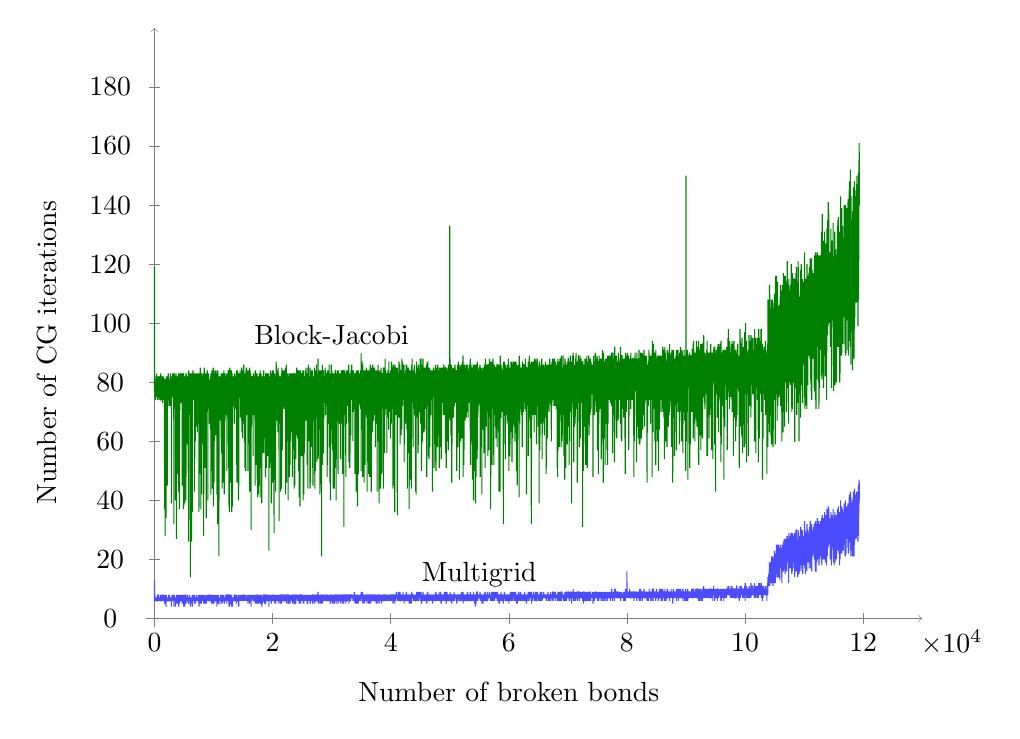
\begin{tikzpicture}[scale=0.75]			

\draw[very thin, color=gray, ->] (-0.15, 0) -- (13, 0);
\draw[very thin, color=gray, ->] (0, -0.15) -- (0, 10);

\draw (13.5, -0.4) node {{$\times 10^4$}};
\draw (6, -1.25) node {{Number of broken bonds}};
\draw[color=white] (-1.5, 4) -- +(90:1) node[midway,sloped,above, color=black]{{Number of CG iterations}};

\draw (3, 4.8) node {{Block-Jacobi}};

\draw (5.5, 0.75) node {{Multigrid}};
  
%Draw Row Ticks
\foreach \pos in {0, 2, ..., 12} {
\draw[very thin, color=gray] (\pos, -0.1) -- (\pos, 0.1);
\draw (\pos, -0.4) node {{\pos}};
}

%Draw Col Ticks
\foreach \pos/\val in {0/0, 1/20, 2/40, 3/60, 4/80, 5/100, 6/120, 7/140, 8/160, 9/180} {
\draw[very thin, color=gray] (-0.1, \pos) -- (0.1, \pos);
\draw (-0.75, \pos) node {{\val}};
}


\draw[color=blue!70]
(0.000000, 0.650000) -- 
(0.001000, 0.300000) -- 
(0.002000, 0.300000) -- 
(0.003000, 0.350000) -- 
(0.004000, 0.400000) -- 
(0.005000, 0.350000) -- 
(0.006000, 0.300000) -- 
(0.007000, 0.300000) -- 
(0.008000, 0.350000) -- 
(0.009000, 0.300000) -- 
(0.010000, 0.350000) -- 
(0.011000, 0.300000) -- 
(0.012000, 0.350000) -- 
(0.013000, 0.300000) -- 
(0.014000, 0.350000) -- 
(0.015000, 0.300000) -- 
(0.016000, 0.350000) -- 
(0.017000, 0.350000) -- 
(0.018000, 0.350000) -- 
(0.019000, 0.350000) -- 
(0.020000, 0.300000) -- 
(0.021000, 0.350000) -- 
(0.022000, 0.350000) -- 
(0.023000, 0.300000) -- 
(0.024000, 0.350000) -- 
(0.025000, 0.300000) -- 
(0.026000, 0.350000) -- 
(0.027000, 0.350000) -- 
(0.028000, 0.350000) -- 
(0.029000, 0.350000) -- 
(0.030000, 0.300000) -- 
(0.031000, 0.300000) -- 
(0.032000, 0.350000) -- 
(0.033000, 0.350000) -- 
(0.034000, 0.300000) -- 
(0.035000, 0.350000) -- 
(0.036000, 0.350000) -- 
(0.037000, 0.350000) -- 
(0.038000, 0.300000) -- 
(0.039000, 0.350000) -- 
(0.040000, 0.350000) -- 
(0.041000, 0.350000) -- 
(0.042000, 0.300000) -- 
(0.043000, 0.300000) -- 
(0.044000, 0.350000) -- 
(0.045000, 0.350000) -- 
(0.046000, 0.300000) -- 
(0.047000, 0.350000) -- 
(0.048000, 0.350000) -- 
(0.049000, 0.350000) -- 
(0.050000, 0.300000) -- 
(0.051000, 0.350000) -- 
(0.052000, 0.400000) -- 
(0.053000, 0.350000) -- 
(0.054000, 0.300000) -- 
(0.055000, 0.300000) -- 
(0.056000, 0.350000) -- 
(0.057000, 0.400000) -- 
(0.058000, 0.350000) -- 
(0.059000, 0.300000) -- 
(0.060000, 0.350000) -- 
(0.061000, 0.350000) -- 
(0.062000, 0.350000) -- 
(0.063000, 0.350000) -- 
(0.064000, 0.350000) -- 
(0.065000, 0.400000) -- 
(0.066000, 0.400000) -- 
(0.067000, 0.350000) -- 
(0.068000, 0.300000) -- 
(0.069000, 0.350000) -- 
(0.070000, 0.400000) -- 
(0.071000, 0.350000) -- 
(0.072000, 0.350000) -- 
(0.073000, 0.350000) -- 
(0.074000, 0.300000) -- 
(0.075000, 0.350000) -- 
(0.076000, 0.300000) -- 
(0.077000, 0.350000) -- 
(0.078000, 0.350000) -- 
(0.079000, 0.350000) -- 
(0.080000, 0.350000) -- 
(0.081000, 0.350000) -- 
(0.082000, 0.300000) -- 
(0.083000, 0.350000) -- 
(0.084000, 0.350000) -- 
(0.085000, 0.350000) -- 
(0.086000, 0.350000) -- 
(0.087000, 0.350000) -- 
(0.088000, 0.350000) -- 
(0.089000, 0.350000) -- 
(0.090000, 0.350000) -- 
(0.091000, 0.350000) -- 
(0.092000, 0.350000) -- 
(0.093000, 0.300000) -- 
(0.094000, 0.350000) -- 
(0.095000, 0.350000) -- 
(0.096000, 0.350000) -- 
(0.097000, 0.300000) -- 
(0.098000, 0.350000) -- 
(0.099000, 0.350000) -- 
(0.100000, 0.300000) -- 
(0.101000, 0.400000) -- 
(0.102000, 0.350000) -- 
(0.103000, 0.300000) -- 
(0.104000, 0.300000) -- 
(0.105000, 0.350000) -- 
(0.106000, 0.350000) -- 
(0.107000, 0.350000) -- 
(0.108000, 0.300000) -- 
(0.109000, 0.350000) -- 
(0.110000, 0.300000) -- 
(0.111000, 0.350000) -- 
(0.112000, 0.300000) -- 
(0.113000, 0.350000) -- 
(0.114000, 0.350000) -- 
(0.115000, 0.350000) -- 
(0.116000, 0.300000) -- 
(0.117000, 0.300000) -- 
(0.118000, 0.300000) -- 
(0.119000, 0.350000) -- 
(0.120000, 0.350000) -- 
(0.121000, 0.400000) -- 
(0.122000, 0.300000) -- 
(0.123000, 0.350000) -- 
(0.124000, 0.350000) -- 
(0.125000, 0.350000) -- 
(0.126000, 0.350000) -- 
(0.127000, 0.350000) -- 
(0.128000, 0.350000) -- 
(0.129000, 0.400000) -- 
(0.130000, 0.350000) -- 
(0.131000, 0.350000) -- 
(0.132000, 0.300000) -- 
(0.133000, 0.350000) -- 
(0.134000, 0.350000) -- 
(0.135000, 0.350000) -- 
(0.136000, 0.350000) -- 
(0.137000, 0.300000) -- 
(0.138000, 0.350000) -- 
(0.139000, 0.300000) -- 
(0.140000, 0.350000) -- 
(0.141000, 0.350000) -- 
(0.142000, 0.350000) -- 
(0.143000, 0.350000) -- 
(0.144000, 0.400000) -- 
(0.145000, 0.400000) -- 
(0.146000, 0.300000) -- 
(0.147000, 0.350000) -- 
(0.148000, 0.350000) -- 
(0.149000, 0.350000) -- 
(0.150000, 0.350000) -- 
(0.151000, 0.350000) -- 
(0.152000, 0.350000) -- 
(0.153000, 0.300000) -- 
(0.154000, 0.350000) -- 
(0.155000, 0.300000) -- 
(0.156000, 0.350000) -- 
(0.157000, 0.350000) -- 
(0.158000, 0.350000) -- 
(0.159000, 0.350000) -- 
(0.160000, 0.350000) -- 
(0.161000, 0.300000) -- 
(0.162000, 0.350000) -- 
(0.163000, 0.350000) -- 
(0.164000, 0.350000) -- 
(0.165000, 0.350000) -- 
(0.166000, 0.350000) -- 
(0.167000, 0.300000) -- 
(0.168000, 0.300000) -- 
(0.169000, 0.350000) -- 
(0.170000, 0.400000) -- 
(0.171000, 0.250000) -- 
(0.172000, 0.350000) -- 
(0.173000, 0.350000) -- 
(0.174000, 0.350000) -- 
(0.175000, 0.350000) -- 
(0.176000, 0.400000) -- 
(0.177000, 0.350000) -- 
(0.178000, 0.350000) -- 
(0.179000, 0.350000) -- 
(0.180000, 0.400000) -- 
(0.181000, 0.250000) -- 
(0.182000, 0.350000) -- 
(0.183000, 0.350000) -- 
(0.184000, 0.350000) -- 
(0.185000, 0.400000) -- 
(0.186000, 0.350000) -- 
(0.187000, 0.300000) -- 
(0.188000, 0.400000) -- 
(0.189000, 0.300000) -- 
(0.190000, 0.300000) -- 
(0.191000, 0.350000) -- 
(0.192000, 0.300000) -- 
(0.193000, 0.350000) -- 
(0.194000, 0.350000) -- 
(0.195000, 0.200000) -- 
(0.196000, 0.350000) -- 
(0.197000, 0.400000) -- 
(0.198000, 0.350000) -- 
(0.199000, 0.350000) -- 
(0.200000, 0.350000) -- 
(0.201000, 0.350000) -- 
(0.202000, 0.400000) -- 
(0.203000, 0.350000) -- 
(0.204000, 0.350000) -- 
(0.205000, 0.350000) -- 
(0.206000, 0.300000) -- 
(0.207000, 0.300000) -- 
(0.208000, 0.350000) -- 
(0.209000, 0.350000) -- 
(0.210000, 0.350000) -- 
(0.211000, 0.350000) -- 
(0.212000, 0.300000) -- 
(0.213000, 0.350000) -- 
(0.214000, 0.300000) -- 
(0.215000, 0.350000) -- 
(0.216000, 0.350000) -- 
(0.217000, 0.300000) -- 
(0.218000, 0.300000) -- 
(0.219000, 0.350000) -- 
(0.220000, 0.350000) -- 
(0.221000, 0.350000) -- 
(0.222000, 0.300000) -- 
(0.223000, 0.350000) -- 
(0.224000, 0.300000) -- 
(0.225000, 0.300000) -- 
(0.226000, 0.300000) -- 
(0.227000, 0.350000) -- 
(0.228000, 0.350000) -- 
(0.229000, 0.350000) -- 
(0.230000, 0.350000) -- 
(0.231000, 0.350000) -- 
(0.232000, 0.300000) -- 
(0.233000, 0.350000) -- 
(0.234000, 0.350000) -- 
(0.235000, 0.350000) -- 
(0.236000, 0.300000) -- 
(0.237000, 0.350000) -- 
(0.238000, 0.350000) -- 
(0.239000, 0.300000) -- 
(0.240000, 0.400000) -- 
(0.241000, 0.350000) -- 
(0.242000, 0.350000) -- 
(0.243000, 0.300000) -- 
(0.244000, 0.300000) -- 
(0.245000, 0.400000) -- 
(0.246000, 0.300000) -- 
(0.247000, 0.350000) -- 
(0.248000, 0.350000) -- 
(0.249000, 0.350000) -- 
(0.250000, 0.300000) -- 
(0.251000, 0.300000) -- 
(0.252000, 0.350000) -- 
(0.253000, 0.350000) -- 
(0.254000, 0.350000) -- 
(0.255000, 0.350000) -- 
(0.256000, 0.400000) -- 
(0.257000, 0.350000) -- 
(0.258000, 0.300000) -- 
(0.259000, 0.300000) -- 
(0.260000, 0.350000) -- 
(0.261000, 0.300000) -- 
(0.262000, 0.300000) -- 
(0.263000, 0.350000) -- 
(0.264000, 0.350000) -- 
(0.265000, 0.300000) -- 
(0.266000, 0.350000) -- 
(0.267000, 0.300000) -- 
(0.268000, 0.350000) -- 
(0.269000, 0.350000) -- 
(0.270000, 0.350000) -- 
(0.271000, 0.350000) -- 
(0.272000, 0.350000) -- 
(0.273000, 0.350000) -- 
(0.274000, 0.350000) -- 
(0.275000, 0.350000) -- 
(0.276000, 0.350000) -- 
(0.277000, 0.350000) -- 
(0.278000, 0.350000) -- 
(0.279000, 0.350000) -- 
(0.280000, 0.350000) -- 
(0.281000, 0.300000) -- 
(0.282000, 0.300000) -- 
(0.283000, 0.350000) -- 
(0.284000, 0.350000) -- 
(0.285000, 0.300000) -- 
(0.286000, 0.200000) -- 
(0.287000, 0.350000) -- 
(0.288000, 0.300000) -- 
(0.289000, 0.350000) -- 
(0.290000, 0.300000) -- 
(0.291000, 0.300000) -- 
(0.292000, 0.350000) -- 
(0.293000, 0.300000) -- 
(0.294000, 0.350000) -- 
(0.295000, 0.350000) -- 
(0.296000, 0.350000) -- 
(0.297000, 0.350000) -- 
(0.298000, 0.400000) -- 
(0.299000, 0.350000) -- 
(0.300000, 0.350000) -- 
(0.301000, 0.350000) -- 
(0.302000, 0.350000) -- 
(0.303000, 0.350000) -- 
(0.304000, 0.350000) -- 
(0.305000, 0.350000) -- 
(0.306000, 0.350000) -- 
(0.307000, 0.350000) -- 
(0.308000, 0.350000) -- 
(0.309000, 0.350000) -- 
(0.310000, 0.400000) -- 
(0.311000, 0.300000) -- 
(0.312000, 0.350000) -- 
(0.313000, 0.350000) -- 
(0.314000, 0.300000) -- 
(0.315000, 0.350000) -- 
(0.316000, 0.300000) -- 
(0.317000, 0.350000) -- 
(0.318000, 0.300000) -- 
(0.319000, 0.350000) -- 
(0.320000, 0.300000) -- 
(0.321000, 0.350000) -- 
(0.322000, 0.350000) -- 
(0.323000, 0.300000) -- 
(0.324000, 0.400000) -- 
(0.325000, 0.350000) -- 
(0.326000, 0.350000) -- 
(0.327000, 0.350000) -- 
(0.328000, 0.200000) -- 
(0.329000, 0.350000) -- 
(0.330000, 0.300000) -- 
(0.331000, 0.350000) -- 
(0.332000, 0.350000) -- 
(0.333000, 0.350000) -- 
(0.334000, 0.350000) -- 
(0.335000, 0.350000) -- 
(0.336000, 0.350000) -- 
(0.337000, 0.350000) -- 
(0.338000, 0.350000) -- 
(0.339000, 0.400000) -- 
(0.340000, 0.350000) -- 
(0.341000, 0.300000) -- 
(0.342000, 0.350000) -- 
(0.343000, 0.350000) -- 
(0.344000, 0.350000) -- 
(0.345000, 0.300000) -- 
(0.346000, 0.300000) -- 
(0.347000, 0.350000) -- 
(0.348000, 0.300000) -- 
(0.349000, 0.300000) -- 
(0.350000, 0.300000) -- 
(0.351000, 0.350000) -- 
(0.352000, 0.350000) -- 
(0.353000, 0.300000) -- 
(0.354000, 0.350000) -- 
(0.355000, 0.200000) -- 
(0.356000, 0.350000) -- 
(0.357000, 0.350000) -- 
(0.358000, 0.300000) -- 
(0.359000, 0.350000) -- 
(0.360000, 0.350000) -- 
(0.361000, 0.300000) -- 
(0.362000, 0.350000) -- 
(0.363000, 0.350000) -- 
(0.364000, 0.350000) -- 
(0.365000, 0.350000) -- 
(0.366000, 0.350000) -- 
(0.367000, 0.300000) -- 
(0.368000, 0.300000) -- 
(0.369000, 0.350000) -- 
(0.370000, 0.300000) -- 
(0.371000, 0.350000) -- 
(0.372000, 0.350000) -- 
(0.373000, 0.250000) -- 
(0.374000, 0.300000) -- 
(0.375000, 0.350000) -- 
(0.376000, 0.350000) -- 
(0.377000, 0.350000) -- 
(0.378000, 0.400000) -- 
(0.379000, 0.300000) -- 
(0.380000, 0.350000) -- 
(0.381000, 0.300000) -- 
(0.382000, 0.350000) -- 
(0.383000, 0.350000) -- 
(0.384000, 0.300000) -- 
(0.385000, 0.350000) -- 
(0.386000, 0.350000) -- 
(0.387000, 0.350000) -- 
(0.388000, 0.400000) -- 
(0.389000, 0.350000) -- 
(0.390000, 0.250000) -- 
(0.391000, 0.350000) -- 
(0.392000, 0.350000) -- 
(0.393000, 0.350000) -- 
(0.394000, 0.300000) -- 
(0.395000, 0.350000) -- 
(0.396000, 0.350000) -- 
(0.397000, 0.350000) -- 
(0.398000, 0.350000) -- 
(0.399000, 0.300000) -- 
(0.400000, 0.350000) -- 
(0.401000, 0.350000) -- 
(0.402000, 0.350000) -- 
(0.403000, 0.350000) -- 
(0.404000, 0.350000) -- 
(0.405000, 0.350000) -- 
(0.406000, 0.400000) -- 
(0.407000, 0.350000) -- 
(0.408000, 0.350000) -- 
(0.409000, 0.300000) -- 
(0.410000, 0.300000) -- 
(0.411000, 0.200000) -- 
(0.412000, 0.350000) -- 
(0.413000, 0.350000) -- 
(0.414000, 0.300000) -- 
(0.415000, 0.300000) -- 
(0.416000, 0.350000) -- 
(0.417000, 0.350000) -- 
(0.418000, 0.350000) -- 
(0.419000, 0.350000) -- 
(0.420000, 0.350000) -- 
(0.421000, 0.250000) -- 
(0.422000, 0.300000) -- 
(0.423000, 0.350000) -- 
(0.424000, 0.300000) -- 
(0.425000, 0.350000) -- 
(0.426000, 0.300000) -- 
(0.427000, 0.350000) -- 
(0.428000, 0.300000) -- 
(0.429000, 0.300000) -- 
(0.430000, 0.350000) -- 
(0.431000, 0.300000) -- 
(0.432000, 0.400000) -- 
(0.433000, 0.300000) -- 
(0.434000, 0.350000) -- 
(0.435000, 0.350000) -- 
(0.436000, 0.350000) -- 
(0.437000, 0.300000) -- 
(0.438000, 0.400000) -- 
(0.439000, 0.350000) -- 
(0.440000, 0.300000) -- 
(0.441000, 0.350000) -- 
(0.442000, 0.300000) -- 
(0.443000, 0.350000) -- 
(0.444000, 0.300000) -- 
(0.445000, 0.350000) -- 
(0.446000, 0.350000) -- 
(0.447000, 0.300000) -- 
(0.448000, 0.300000) -- 
(0.449000, 0.300000) -- 
(0.450000, 0.350000) -- 
(0.451000, 0.350000) -- 
(0.452000, 0.300000) -- 
(0.453000, 0.350000) -- 
(0.454000, 0.300000) -- 
(0.455000, 0.350000) -- 
(0.456000, 0.300000) -- 
(0.457000, 0.350000) -- 
(0.458000, 0.350000) -- 
(0.459000, 0.350000) -- 
(0.460000, 0.350000) -- 
(0.461000, 0.350000) -- 
(0.462000, 0.400000) -- 
(0.463000, 0.350000) -- 
(0.464000, 0.350000) -- 
(0.465000, 0.350000) -- 
(0.466000, 0.300000) -- 
(0.467000, 0.300000) -- 
(0.468000, 0.350000) -- 
(0.469000, 0.350000) -- 
(0.470000, 0.400000) -- 
(0.471000, 0.250000) -- 
(0.472000, 0.350000) -- 
(0.473000, 0.350000) -- 
(0.474000, 0.300000) -- 
(0.475000, 0.350000) -- 
(0.476000, 0.350000) -- 
(0.477000, 0.350000) -- 
(0.478000, 0.300000) -- 
(0.479000, 0.350000) -- 
(0.480000, 0.350000) -- 
(0.481000, 0.400000) -- 
(0.482000, 0.350000) -- 
(0.483000, 0.350000) -- 
(0.484000, 0.350000) -- 
(0.485000, 0.400000) -- 
(0.486000, 0.350000) -- 
(0.487000, 0.350000) -- 
(0.488000, 0.350000) -- 
(0.489000, 0.250000) -- 
(0.490000, 0.350000) -- 
(0.491000, 0.350000) -- 
(0.492000, 0.350000) -- 
(0.493000, 0.350000) -- 
(0.494000, 0.300000) -- 
(0.495000, 0.400000) -- 
(0.496000, 0.200000) -- 
(0.497000, 0.300000) -- 
(0.498000, 0.350000) -- 
(0.499000, 0.350000) -- 
(0.500000, 0.400000) -- 
(0.501000, 0.350000) -- 
(0.502000, 0.350000) -- 
(0.503000, 0.350000) -- 
(0.504000, 0.350000) -- 
(0.505000, 0.300000) -- 
(0.506000, 0.350000) -- 
(0.507000, 0.200000) -- 
(0.508000, 0.300000) -- 
(0.509000, 0.300000) -- 
(0.510000, 0.300000) -- 
(0.511000, 0.350000) -- 
(0.512000, 0.200000) -- 
(0.513000, 0.350000) -- 
(0.514000, 0.350000) -- 
(0.515000, 0.350000) -- 
(0.516000, 0.400000) -- 
(0.517000, 0.350000) -- 
(0.518000, 0.350000) -- 
(0.519000, 0.350000) -- 
(0.520000, 0.350000) -- 
(0.521000, 0.300000) -- 
(0.522000, 0.350000) -- 
(0.523000, 0.350000) -- 
(0.524000, 0.350000) -- 
(0.525000, 0.350000) -- 
(0.526000, 0.400000) -- 
(0.527000, 0.400000) -- 
(0.528000, 0.300000) -- 
(0.529000, 0.350000) -- 
(0.530000, 0.300000) -- 
(0.531000, 0.350000) -- 
(0.532000, 0.350000) -- 
(0.533000, 0.250000) -- 
(0.534000, 0.350000) -- 
(0.535000, 0.300000) -- 
(0.536000, 0.350000) -- 
(0.537000, 0.300000) -- 
(0.538000, 0.350000) -- 
(0.539000, 0.350000) -- 
(0.540000, 0.300000) -- 
(0.541000, 0.350000) -- 
(0.542000, 0.350000) -- 
(0.543000, 0.350000) -- 
(0.544000, 0.350000) -- 
(0.545000, 0.350000) -- 
(0.546000, 0.300000) -- 
(0.547000, 0.300000) -- 
(0.548000, 0.350000) -- 
(0.549000, 0.350000) -- 
(0.550000, 0.300000) -- 
(0.551000, 0.300000) -- 
(0.552000, 0.350000) -- 
(0.553000, 0.350000) -- 
(0.554000, 0.350000) -- 
(0.555000, 0.400000) -- 
(0.556000, 0.300000) -- 
(0.557000, 0.350000) -- 
(0.558000, 0.350000) -- 
(0.559000, 0.350000) -- 
(0.560000, 0.350000) -- 
(0.561000, 0.350000) -- 
(0.562000, 0.300000) -- 
(0.563000, 0.300000) -- 
(0.564000, 0.300000) -- 
(0.565000, 0.300000) -- 
(0.566000, 0.350000) -- 
(0.567000, 0.350000) -- 
(0.568000, 0.350000) -- 
(0.569000, 0.300000) -- 
(0.570000, 0.350000) -- 
(0.571000, 0.300000) -- 
(0.572000, 0.300000) -- 
(0.573000, 0.250000) -- 
(0.574000, 0.300000) -- 
(0.575000, 0.350000) -- 
(0.576000, 0.300000) -- 
(0.577000, 0.300000) -- 
(0.578000, 0.250000) -- 
(0.579000, 0.350000) -- 
(0.580000, 0.350000) -- 
(0.581000, 0.350000) -- 
(0.582000, 0.350000) -- 
(0.583000, 0.350000) -- 
(0.584000, 0.300000) -- 
(0.585000, 0.350000) -- 
(0.586000, 0.350000) -- 
(0.587000, 0.350000) -- 
(0.588000, 0.400000) -- 
(0.589000, 0.300000) -- 
(0.590000, 0.350000) -- 
(0.591000, 0.300000) -- 
(0.592000, 0.400000) -- 
(0.593000, 0.350000) -- 
(0.594000, 0.350000) -- 
(0.595000, 0.350000) -- 
(0.596000, 0.400000) -- 
(0.597000, 0.350000) -- 
(0.598000, 0.300000) -- 
(0.599000, 0.350000) -- 
(0.600000, 0.350000) -- 
(0.601000, 0.350000) -- 
(0.602000, 0.350000) -- 
(0.603000, 0.350000) -- 
(0.604000, 0.350000) -- 
(0.605000, 0.350000) -- 
(0.606000, 0.300000) -- 
(0.607000, 0.200000) -- 
(0.608000, 0.350000) -- 
(0.609000, 0.350000) -- 
(0.610000, 0.300000) -- 
(0.611000, 0.350000) -- 
(0.612000, 0.350000) -- 
(0.613000, 0.350000) -- 
(0.614000, 0.350000) -- 
(0.615000, 0.350000) -- 
(0.616000, 0.350000) -- 
(0.617000, 0.350000) -- 
(0.618000, 0.350000) -- 
(0.619000, 0.350000) -- 
(0.620000, 0.300000) -- 
(0.621000, 0.350000) -- 
(0.622000, 0.350000) -- 
(0.623000, 0.350000) -- 
(0.624000, 0.350000) -- 
(0.625000, 0.350000) -- 
(0.626000, 0.350000) -- 
(0.627000, 0.250000) -- 
(0.628000, 0.350000) -- 
(0.629000, 0.350000) -- 
(0.630000, 0.350000) -- 
(0.631000, 0.350000) -- 
(0.632000, 0.350000) -- 
(0.633000, 0.300000) -- 
(0.634000, 0.300000) -- 
(0.635000, 0.350000) -- 
(0.636000, 0.250000) -- 
(0.637000, 0.350000) -- 
(0.638000, 0.400000) -- 
(0.639000, 0.200000) -- 
(0.640000, 0.350000) -- 
(0.641000, 0.300000) -- 
(0.642000, 0.350000) -- 
(0.643000, 0.350000) -- 
(0.644000, 0.400000) -- 
(0.645000, 0.350000) -- 
(0.646000, 0.350000) -- 
(0.647000, 0.350000) -- 
(0.648000, 0.350000) -- 
(0.649000, 0.350000) -- 
(0.650000, 0.350000) -- 
(0.651000, 0.400000) -- 
(0.652000, 0.300000) -- 
(0.653000, 0.350000) -- 
(0.654000, 0.300000) -- 
(0.655000, 0.350000) -- 
(0.656000, 0.350000) -- 
(0.657000, 0.350000) -- 
(0.658000, 0.350000) -- 
(0.659000, 0.350000) -- 
(0.660000, 0.300000) -- 
(0.661000, 0.350000) -- 
(0.662000, 0.300000) -- 
(0.663000, 0.350000) -- 
(0.664000, 0.400000) -- 
(0.665000, 0.350000) -- 
(0.666000, 0.350000) -- 
(0.667000, 0.350000) -- 
(0.668000, 0.350000) -- 
(0.669000, 0.350000) -- 
(0.670000, 0.350000) -- 
(0.671000, 0.350000) -- 
(0.672000, 0.350000) -- 
(0.673000, 0.350000) -- 
(0.674000, 0.350000) -- 
(0.675000, 0.350000) -- 
(0.676000, 0.250000) -- 
(0.677000, 0.400000) -- 
(0.678000, 0.300000) -- 
(0.679000, 0.350000) -- 
(0.680000, 0.350000) -- 
(0.681000, 0.300000) -- 
(0.682000, 0.350000) -- 
(0.683000, 0.300000) -- 
(0.684000, 0.350000) -- 
(0.685000, 0.300000) -- 
(0.686000, 0.300000) -- 
(0.687000, 0.350000) -- 
(0.688000, 0.300000) -- 
(0.689000, 0.350000) -- 
(0.690000, 0.250000) -- 
(0.691000, 0.350000) -- 
(0.692000, 0.350000) -- 
(0.693000, 0.350000) -- 
(0.694000, 0.300000) -- 
(0.695000, 0.350000) -- 
(0.696000, 0.350000) -- 
(0.697000, 0.350000) -- 
(0.698000, 0.350000) -- 
(0.699000, 0.350000) -- 
(0.700000, 0.350000) -- 
(0.701000, 0.350000) -- 
(0.702000, 0.300000) -- 
(0.703000, 0.350000) -- 
(0.704000, 0.300000) -- 
(0.705000, 0.350000) -- 
(0.706000, 0.300000) -- 
(0.707000, 0.350000) -- 
(0.708000, 0.350000) -- 
(0.709000, 0.350000) -- 
(0.710000, 0.400000) -- 
(0.711000, 0.350000) -- 
(0.712000, 0.350000) -- 
(0.713000, 0.300000) -- 
(0.714000, 0.350000) -- 
(0.715000, 0.350000) -- 
(0.716000, 0.300000) -- 
(0.717000, 0.350000) -- 
(0.718000, 0.300000) -- 
(0.719000, 0.300000) -- 
(0.720000, 0.350000) -- 
(0.721000, 0.350000) -- 
(0.722000, 0.300000) -- 
(0.723000, 0.350000) -- 
(0.724000, 0.350000) -- 
(0.725000, 0.350000) -- 
(0.726000, 0.350000) -- 
(0.727000, 0.300000) -- 
(0.728000, 0.350000) -- 
(0.729000, 0.300000) -- 
(0.730000, 0.350000) -- 
(0.731000, 0.350000) -- 
(0.732000, 0.300000) -- 
(0.733000, 0.350000) -- 
(0.734000, 0.350000) -- 
(0.735000, 0.350000) -- 
(0.736000, 0.350000) -- 
(0.737000, 0.300000) -- 
(0.738000, 0.350000) -- 
(0.739000, 0.350000) -- 
(0.740000, 0.400000) -- 
(0.741000, 0.350000) -- 
(0.742000, 0.350000) -- 
(0.743000, 0.350000) -- 
(0.744000, 0.300000) -- 
(0.745000, 0.300000) -- 
(0.746000, 0.350000) -- 
(0.747000, 0.350000) -- 
(0.748000, 0.350000) -- 
(0.749000, 0.350000) -- 
(0.750000, 0.300000) -- 
(0.751000, 0.300000) -- 
(0.752000, 0.300000) -- 
(0.753000, 0.200000) -- 
(0.754000, 0.350000) -- 
(0.755000, 0.350000) -- 
(0.756000, 0.350000) -- 
(0.757000, 0.300000) -- 
(0.758000, 0.350000) -- 
(0.759000, 0.300000) -- 
(0.760000, 0.400000) -- 
(0.761000, 0.350000) -- 
(0.762000, 0.300000) -- 
(0.763000, 0.350000) -- 
(0.764000, 0.350000) -- 
(0.765000, 0.300000) -- 
(0.766000, 0.350000) -- 
(0.767000, 0.350000) -- 
(0.768000, 0.350000) -- 
(0.769000, 0.300000) -- 
(0.770000, 0.350000) -- 
(0.771000, 0.350000) -- 
(0.772000, 0.250000) -- 
(0.773000, 0.300000) -- 
(0.774000, 0.350000) -- 
(0.775000, 0.350000) -- 
(0.776000, 0.400000) -- 
(0.777000, 0.300000) -- 
(0.778000, 0.400000) -- 
(0.779000, 0.350000) -- 
(0.780000, 0.350000) -- 
(0.781000, 0.350000) -- 
(0.782000, 0.350000) -- 
(0.783000, 0.400000) -- 
(0.784000, 0.350000) -- 
(0.785000, 0.250000) -- 
(0.786000, 0.350000) -- 
(0.787000, 0.350000) -- 
(0.788000, 0.400000) -- 
(0.789000, 0.350000) -- 
(0.790000, 0.350000) -- 
(0.791000, 0.300000) -- 
(0.792000, 0.350000) -- 
(0.793000, 0.300000) -- 
(0.794000, 0.250000) -- 
(0.795000, 0.400000) -- 
(0.796000, 0.350000) -- 
(0.797000, 0.350000) -- 
(0.798000, 0.350000) -- 
(0.799000, 0.400000) -- 
(0.800000, 0.350000) -- 
(0.801000, 0.350000) -- 
(0.802000, 0.400000) -- 
(0.803000, 0.300000) -- 
(0.804000, 0.350000) -- 
(0.805000, 0.350000) -- 
(0.806000, 0.350000) -- 
(0.807000, 0.350000) -- 
(0.808000, 0.350000) -- 
(0.809000, 0.350000) -- 
(0.810000, 0.350000) -- 
(0.811000, 0.400000) -- 
(0.812000, 0.300000) -- 
(0.813000, 0.350000) -- 
(0.814000, 0.300000) -- 
(0.815000, 0.350000) -- 
(0.816000, 0.350000) -- 
(0.817000, 0.350000) -- 
(0.818000, 0.350000) -- 
(0.819000, 0.350000) -- 
(0.820000, 0.350000) -- 
(0.821000, 0.400000) -- 
(0.822000, 0.350000) -- 
(0.823000, 0.350000) -- 
(0.824000, 0.350000) -- 
(0.825000, 0.350000) -- 
(0.826000, 0.300000) -- 
(0.827000, 0.300000) -- 
(0.828000, 0.350000) -- 
(0.829000, 0.400000) -- 
(0.830000, 0.350000) -- 
(0.831000, 0.300000) -- 
(0.832000, 0.350000) -- 
(0.833000, 0.250000) -- 
(0.834000, 0.350000) -- 
(0.835000, 0.350000) -- 
(0.836000, 0.350000) -- 
(0.837000, 0.250000) -- 
(0.838000, 0.350000) -- 
(0.839000, 0.300000) -- 
(0.840000, 0.350000) -- 
(0.841000, 0.300000) -- 
(0.842000, 0.350000) -- 
(0.843000, 0.350000) -- 
(0.844000, 0.350000) -- 
(0.845000, 0.350000) -- 
(0.846000, 0.350000) -- 
(0.847000, 0.350000) -- 
(0.848000, 0.350000) -- 
(0.849000, 0.400000) -- 
(0.850000, 0.350000) -- 
(0.851000, 0.300000) -- 
(0.852000, 0.300000) -- 
(0.853000, 0.350000) -- 
(0.854000, 0.300000) -- 
(0.855000, 0.350000) -- 
(0.856000, 0.350000) -- 
(0.857000, 0.350000) -- 
(0.858000, 0.350000) -- 
(0.859000, 0.250000) -- 
(0.860000, 0.300000) -- 
(0.861000, 0.350000) -- 
(0.862000, 0.300000) -- 
(0.863000, 0.350000) -- 
(0.864000, 0.300000) -- 
(0.865000, 0.350000) -- 
(0.866000, 0.300000) -- 
(0.867000, 0.300000) -- 
(0.868000, 0.300000) -- 
(0.869000, 0.350000) -- 
(0.870000, 0.350000) -- 
(0.871000, 0.350000) -- 
(0.872000, 0.350000) -- 
(0.873000, 0.350000) -- 
(0.874000, 0.400000) -- 
(0.875000, 0.300000) -- 
(0.876000, 0.350000) -- 
(0.877000, 0.250000) -- 
(0.878000, 0.350000) -- 
(0.879000, 0.350000) -- 
(0.880000, 0.350000) -- 
(0.881000, 0.350000) -- 
(0.882000, 0.350000) -- 
(0.883000, 0.350000) -- 
(0.884000, 0.300000) -- 
(0.885000, 0.350000) -- 
(0.886000, 0.350000) -- 
(0.887000, 0.350000) -- 
(0.888000, 0.400000) -- 
(0.889000, 0.350000) -- 
(0.890000, 0.350000) -- 
(0.891000, 0.350000) -- 
(0.892000, 0.300000) -- 
(0.893000, 0.350000) -- 
(0.894000, 0.350000) -- 
(0.895000, 0.350000) -- 
(0.896000, 0.350000) -- 
(0.897000, 0.350000) -- 
(0.898000, 0.350000) -- 
(0.899000, 0.300000) -- 
(0.900000, 0.350000) -- 
(0.901000, 0.300000) -- 
(0.902000, 0.350000) -- 
(0.903000, 0.350000) -- 
(0.904000, 0.300000) -- 
(0.905000, 0.400000) -- 
(0.906000, 0.350000) -- 
(0.907000, 0.350000) -- 
(0.908000, 0.350000) -- 
(0.909000, 0.350000) -- 
(0.910000, 0.350000) -- 
(0.911000, 0.350000) -- 
(0.912000, 0.350000) -- 
(0.913000, 0.350000) -- 
(0.914000, 0.300000) -- 
(0.915000, 0.350000) -- 
(0.916000, 0.350000) -- 
(0.917000, 0.350000) -- 
(0.918000, 0.350000) -- 
(0.919000, 0.350000) -- 
(0.920000, 0.350000) -- 
(0.921000, 0.350000) -- 
(0.922000, 0.300000) -- 
(0.923000, 0.350000) -- 
(0.924000, 0.300000) -- 
(0.925000, 0.300000) -- 
(0.926000, 0.400000) -- 
(0.927000, 0.400000) -- 
(0.928000, 0.300000) -- 
(0.929000, 0.350000) -- 
(0.930000, 0.350000) -- 
(0.931000, 0.350000) -- 
(0.932000, 0.350000) -- 
(0.933000, 0.350000) -- 
(0.934000, 0.350000) -- 
(0.935000, 0.350000) -- 
(0.936000, 0.350000) -- 
(0.937000, 0.400000) -- 
(0.938000, 0.300000) -- 
(0.939000, 0.350000) -- 
(0.940000, 0.300000) -- 
(0.941000, 0.350000) -- 
(0.942000, 0.400000) -- 
(0.943000, 0.350000) -- 
(0.944000, 0.350000) -- 
(0.945000, 0.300000) -- 
(0.946000, 0.350000) -- 
(0.947000, 0.300000) -- 
(0.948000, 0.300000) -- 
(0.949000, 0.350000) -- 
(0.950000, 0.350000) -- 
(0.951000, 0.400000) -- 
(0.952000, 0.350000) -- 
(0.953000, 0.350000) -- 
(0.954000, 0.350000) -- 
(0.955000, 0.350000) -- 
(0.956000, 0.300000) -- 
(0.957000, 0.350000) -- 
(0.958000, 0.400000) -- 
(0.959000, 0.300000) -- 
(0.960000, 0.350000) -- 
(0.961000, 0.300000) -- 
(0.962000, 0.350000) -- 
(0.963000, 0.250000) -- 
(0.964000, 0.350000) -- 
(0.965000, 0.350000) -- 
(0.966000, 0.350000) -- 
(0.967000, 0.350000) -- 
(0.968000, 0.350000) -- 
(0.969000, 0.300000) -- 
(0.970000, 0.350000) -- 
(0.971000, 0.400000) -- 
(0.972000, 0.350000) -- 
(0.973000, 0.350000) -- 
(0.974000, 0.350000) -- 
(0.975000, 0.350000) -- 
(0.976000, 0.350000) -- 
(0.977000, 0.300000) -- 
(0.978000, 0.350000) -- 
(0.979000, 0.350000) -- 
(0.980000, 0.250000) -- 
(0.981000, 0.300000) -- 
(0.982000, 0.350000) -- 
(0.983000, 0.350000) -- 
(0.984000, 0.350000) -- 
(0.985000, 0.350000) -- 
(0.986000, 0.350000) -- 
(0.987000, 0.350000) -- 
(0.988000, 0.350000) -- 
(0.989000, 0.350000) -- 
(0.990000, 0.350000) -- 
(0.991000, 0.350000) -- 
(0.992000, 0.350000) -- 
(0.993000, 0.350000) -- 
(0.994000, 0.250000) -- 
(0.995000, 0.400000) -- 
(0.996000, 0.350000) -- 
(0.997000, 0.350000) -- 
(0.998000, 0.250000) -- 
(0.999000, 0.350000) -- 
(1.000000, 0.350000) -- 
(1.001000, 0.350000) -- 
(1.002000, 0.350000) -- 
(1.003000, 0.350000) -- 
(1.004000, 0.350000) -- 
(1.005000, 0.300000) -- 
(1.006000, 0.350000) -- 
(1.007000, 0.400000) -- 
(1.008000, 0.250000) -- 
(1.009000, 0.350000) -- 
(1.010000, 0.350000) -- 
(1.011000, 0.350000) -- 
(1.012000, 0.350000) -- 
(1.013000, 0.350000) -- 
(1.014000, 0.350000) -- 
(1.015000, 0.350000) -- 
(1.016000, 0.300000) -- 
(1.017000, 0.350000) -- 
(1.018000, 0.300000) -- 
(1.019000, 0.350000) -- 
(1.020000, 0.350000) -- 
(1.021000, 0.350000) -- 
(1.022000, 0.350000) -- 
(1.023000, 0.350000) -- 
(1.024000, 0.400000) -- 
(1.025000, 0.300000) -- 
(1.026000, 0.350000) -- 
(1.027000, 0.350000) -- 
(1.028000, 0.300000) -- 
(1.029000, 0.350000) -- 
(1.030000, 0.350000) -- 
(1.031000, 0.350000) -- 
(1.032000, 0.350000) -- 
(1.033000, 0.350000) -- 
(1.034000, 0.400000) -- 
(1.035000, 0.350000) -- 
(1.036000, 0.350000) -- 
(1.037000, 0.400000) -- 
(1.038000, 0.300000) -- 
(1.039000, 0.300000) -- 
(1.040000, 0.350000) -- 
(1.041000, 0.350000) -- 
(1.042000, 0.300000) -- 
(1.043000, 0.300000) -- 
(1.044000, 0.350000) -- 
(1.045000, 0.300000) -- 
(1.046000, 0.350000) -- 
(1.047000, 0.350000) -- 
(1.048000, 0.300000) -- 
(1.049000, 0.350000) -- 
(1.050000, 0.400000) -- 
(1.051000, 0.300000) -- 
(1.052000, 0.350000) -- 
(1.053000, 0.400000) -- 
(1.054000, 0.300000) -- 
(1.055000, 0.350000) -- 
(1.056000, 0.300000) -- 
(1.057000, 0.200000) -- 
(1.058000, 0.400000) -- 
(1.059000, 0.350000) -- 
(1.060000, 0.350000) -- 
(1.061000, 0.350000) -- 
(1.062000, 0.400000) -- 
(1.063000, 0.350000) -- 
(1.064000, 0.350000) -- 
(1.065000, 0.350000) -- 
(1.066000, 0.350000) -- 
(1.067000, 0.350000) -- 
(1.068000, 0.350000) -- 
(1.069000, 0.350000) -- 
(1.070000, 0.350000) -- 
(1.071000, 0.350000) -- 
(1.072000, 0.250000) -- 
(1.073000, 0.350000) -- 
(1.074000, 0.400000) -- 
(1.075000, 0.350000) -- 
(1.076000, 0.400000) -- 
(1.077000, 0.350000) -- 
(1.078000, 0.350000) -- 
(1.079000, 0.350000) -- 
(1.080000, 0.350000) -- 
(1.081000, 0.350000) -- 
(1.082000, 0.400000) -- 
(1.083000, 0.350000) -- 
(1.084000, 0.350000) -- 
(1.085000, 0.350000) -- 
(1.086000, 0.300000) -- 
(1.087000, 0.350000) -- 
(1.088000, 0.350000) -- 
(1.089000, 0.300000) -- 
(1.090000, 0.300000) -- 
(1.091000, 0.250000) -- 
(1.092000, 0.250000) -- 
(1.093000, 0.350000) -- 
(1.094000, 0.350000) -- 
(1.095000, 0.350000) -- 
(1.096000, 0.350000) -- 
(1.097000, 0.350000) -- 
(1.098000, 0.350000) -- 
(1.099000, 0.350000) -- 
(1.100000, 0.350000) -- 
(1.101000, 0.350000) -- 
(1.102000, 0.350000) -- 
(1.103000, 0.350000) -- 
(1.104000, 0.350000) -- 
(1.105000, 0.350000) -- 
(1.106000, 0.350000) -- 
(1.107000, 0.300000) -- 
(1.108000, 0.350000) -- 
(1.109000, 0.350000) -- 
(1.110000, 0.350000) -- 
(1.111000, 0.350000) -- 
(1.112000, 0.350000) -- 
(1.113000, 0.350000) -- 
(1.114000, 0.350000) -- 
(1.115000, 0.350000) -- 
(1.116000, 0.350000) -- 
(1.117000, 0.350000) -- 
(1.118000, 0.350000) -- 
(1.119000, 0.350000) -- 
(1.120000, 0.400000) -- 
(1.121000, 0.350000) -- 
(1.122000, 0.400000) -- 
(1.123000, 0.350000) -- 
(1.124000, 0.300000) -- 
(1.125000, 0.350000) -- 
(1.126000, 0.350000) -- 
(1.127000, 0.350000) -- 
(1.128000, 0.250000) -- 
(1.129000, 0.400000) -- 
(1.130000, 0.350000) -- 
(1.131000, 0.350000) -- 
(1.132000, 0.350000) -- 
(1.133000, 0.300000) -- 
(1.134000, 0.350000) -- 
(1.135000, 0.350000) -- 
(1.136000, 0.250000) -- 
(1.137000, 0.350000) -- 
(1.138000, 0.350000) -- 
(1.139000, 0.350000) -- 
(1.140000, 0.350000) -- 
(1.141000, 0.350000) -- 
(1.142000, 0.350000) -- 
(1.143000, 0.350000) -- 
(1.144000, 0.300000) -- 
(1.145000, 0.350000) -- 
(1.146000, 0.250000) -- 
(1.147000, 0.350000) -- 
(1.148000, 0.350000) -- 
(1.149000, 0.300000) -- 
(1.150000, 0.350000) -- 
(1.151000, 0.350000) -- 
(1.152000, 0.400000) -- 
(1.153000, 0.350000) -- 
(1.154000, 0.350000) -- 
(1.155000, 0.350000) -- 
(1.156000, 0.350000) -- 
(1.157000, 0.350000) -- 
(1.158000, 0.350000) -- 
(1.159000, 0.350000) -- 
(1.160000, 0.350000) -- 
(1.161000, 0.350000) -- 
(1.162000, 0.350000) -- 
(1.163000, 0.300000) -- 
(1.164000, 0.350000) -- 
(1.165000, 0.400000) -- 
(1.166000, 0.300000) -- 
(1.167000, 0.300000) -- 
(1.168000, 0.350000) -- 
(1.169000, 0.400000) -- 
(1.170000, 0.350000) -- 
(1.171000, 0.350000) -- 
(1.172000, 0.350000) -- 
(1.173000, 0.350000) -- 
(1.174000, 0.350000) -- 
(1.175000, 0.300000) -- 
(1.176000, 0.350000) -- 
(1.177000, 0.350000) -- 
(1.178000, 0.300000) -- 
(1.179000, 0.300000) -- 
(1.180000, 0.350000) -- 
(1.181000, 0.300000) -- 
(1.182000, 0.250000) -- 
(1.183000, 0.350000) -- 
(1.184000, 0.350000) -- 
(1.185000, 0.350000) -- 
(1.186000, 0.300000) -- 
(1.187000, 0.350000) -- 
(1.188000, 0.250000) -- 
(1.189000, 0.350000) -- 
(1.190000, 0.350000) -- 
(1.191000, 0.350000) -- 
(1.192000, 0.300000) -- 
(1.193000, 0.350000) -- 
(1.194000, 0.300000) -- 
(1.195000, 0.350000) -- 
(1.196000, 0.350000) -- 
(1.197000, 0.300000) -- 
(1.198000, 0.300000) -- 
(1.199000, 0.350000) -- 
(1.200000, 0.350000) -- 
(1.201000, 0.350000) -- 
(1.202000, 0.400000) -- 
(1.203000, 0.350000) -- 
(1.204000, 0.400000) -- 
(1.205000, 0.350000) -- 
(1.206000, 0.300000) -- 
(1.207000, 0.350000) -- 
(1.208000, 0.350000) -- 
(1.209000, 0.350000) -- 
(1.210000, 0.350000) -- 
(1.211000, 0.300000) -- 
(1.212000, 0.350000) -- 
(1.213000, 0.350000) -- 
(1.214000, 0.300000) -- 
(1.215000, 0.400000) -- 
(1.216000, 0.350000) -- 
(1.217000, 0.300000) -- 
(1.218000, 0.350000) -- 
(1.219000, 0.350000) -- 
(1.220000, 0.350000) -- 
(1.221000, 0.350000) -- 
(1.222000, 0.350000) -- 
(1.223000, 0.350000) -- 
(1.224000, 0.350000) -- 
(1.225000, 0.350000) -- 
(1.226000, 0.250000) -- 
(1.227000, 0.300000) -- 
(1.228000, 0.400000) -- 
(1.229000, 0.400000) -- 
(1.230000, 0.400000) -- 
(1.231000, 0.350000) -- 
(1.232000, 0.400000) -- 
(1.233000, 0.350000) -- 
(1.234000, 0.350000) -- 
(1.235000, 0.350000) -- 
(1.236000, 0.350000) -- 
(1.237000, 0.350000) -- 
(1.238000, 0.400000) -- 
(1.239000, 0.350000) -- 
(1.240000, 0.300000) -- 
(1.241000, 0.350000) -- 
(1.242000, 0.350000) -- 
(1.243000, 0.350000) -- 
(1.244000, 0.350000) -- 
(1.245000, 0.400000) -- 
(1.246000, 0.300000) -- 
(1.247000, 0.350000) -- 
(1.248000, 0.350000) -- 
(1.249000, 0.400000) -- 
(1.250000, 0.400000) -- 
(1.251000, 0.350000) -- 
(1.252000, 0.350000) -- 
(1.253000, 0.350000) -- 
(1.254000, 0.350000) -- 
(1.255000, 0.350000) -- 
(1.256000, 0.300000) -- 
(1.257000, 0.350000) -- 
(1.258000, 0.350000) -- 
(1.259000, 0.250000) -- 
(1.260000, 0.350000) -- 
(1.261000, 0.350000) -- 
(1.262000, 0.300000) -- 
(1.263000, 0.200000) -- 
(1.264000, 0.300000) -- 
(1.265000, 0.300000) -- 
(1.266000, 0.300000) -- 
(1.267000, 0.350000) -- 
(1.268000, 0.350000) -- 
(1.269000, 0.350000) -- 
(1.270000, 0.200000) -- 
(1.271000, 0.300000) -- 
(1.272000, 0.300000) -- 
(1.273000, 0.350000) -- 
(1.274000, 0.350000) -- 
(1.275000, 0.400000) -- 
(1.276000, 0.350000) -- 
(1.277000, 0.400000) -- 
(1.278000, 0.350000) -- 
(1.279000, 0.400000) -- 
(1.280000, 0.400000) -- 
(1.281000, 0.350000) -- 
(1.282000, 0.350000) -- 
(1.283000, 0.250000) -- 
(1.284000, 0.250000) -- 
(1.285000, 0.350000) -- 
(1.286000, 0.350000) -- 
(1.287000, 0.250000) -- 
(1.288000, 0.350000) -- 
(1.289000, 0.350000) -- 
(1.290000, 0.300000) -- 
(1.291000, 0.400000) -- 
(1.292000, 0.350000) -- 
(1.293000, 0.350000) -- 
(1.294000, 0.250000) -- 
(1.295000, 0.300000) -- 
(1.296000, 0.350000) -- 
(1.297000, 0.350000) -- 
(1.298000, 0.350000) -- 
(1.299000, 0.400000) -- 
(1.300000, 0.350000) -- 
(1.301000, 0.400000) -- 
(1.302000, 0.350000) -- 
(1.303000, 0.350000) -- 
(1.304000, 0.300000) -- 
(1.305000, 0.350000) -- 
(1.306000, 0.350000) -- 
(1.307000, 0.400000) -- 
(1.308000, 0.300000) -- 
(1.309000, 0.200000) -- 
(1.310000, 0.350000) -- 
(1.311000, 0.350000) -- 
(1.312000, 0.300000) -- 
(1.313000, 0.350000) -- 
(1.314000, 0.350000) -- 
(1.315000, 0.350000) -- 
(1.316000, 0.350000) -- 
(1.317000, 0.350000) -- 
(1.318000, 0.350000) -- 
(1.319000, 0.200000) -- 
(1.320000, 0.350000) -- 
(1.321000, 0.300000) -- 
(1.322000, 0.350000) -- 
(1.323000, 0.350000) -- 
(1.324000, 0.350000) -- 
(1.325000, 0.350000) -- 
(1.326000, 0.350000) -- 
(1.327000, 0.350000) -- 
(1.328000, 0.350000) -- 
(1.329000, 0.300000) -- 
(1.330000, 0.350000) -- 
(1.331000, 0.350000) -- 
(1.332000, 0.300000) -- 
(1.333000, 0.350000) -- 
(1.334000, 0.350000) -- 
(1.335000, 0.350000) -- 
(1.336000, 0.350000) -- 
(1.337000, 0.350000) -- 
(1.338000, 0.300000) -- 
(1.339000, 0.300000) -- 
(1.340000, 0.350000) -- 
(1.341000, 0.350000) -- 
(1.342000, 0.350000) -- 
(1.343000, 0.350000) -- 
(1.344000, 0.350000) -- 
(1.345000, 0.350000) -- 
(1.346000, 0.350000) -- 
(1.347000, 0.350000) -- 
(1.348000, 0.350000) -- 
(1.349000, 0.400000) -- 
(1.350000, 0.350000) -- 
(1.351000, 0.350000) -- 
(1.352000, 0.350000) -- 
(1.353000, 0.300000) -- 
(1.354000, 0.400000) -- 
(1.355000, 0.350000) -- 
(1.356000, 0.350000) -- 
(1.357000, 0.350000) -- 
(1.358000, 0.400000) -- 
(1.359000, 0.400000) -- 
(1.360000, 0.350000) -- 
(1.361000, 0.350000) -- 
(1.362000, 0.350000) -- 
(1.363000, 0.350000) -- 
(1.364000, 0.350000) -- 
(1.365000, 0.350000) -- 
(1.366000, 0.350000) -- 
(1.367000, 0.350000) -- 
(1.368000, 0.350000) -- 
(1.369000, 0.350000) -- 
(1.370000, 0.350000) -- 
(1.371000, 0.350000) -- 
(1.372000, 0.350000) -- 
(1.373000, 0.300000) -- 
(1.374000, 0.300000) -- 
(1.375000, 0.400000) -- 
(1.376000, 0.350000) -- 
(1.377000, 0.350000) -- 
(1.378000, 0.350000) -- 
(1.379000, 0.300000) -- 
(1.380000, 0.400000) -- 
(1.381000, 0.300000) -- 
(1.382000, 0.300000) -- 
(1.383000, 0.350000) -- 
(1.384000, 0.350000) -- 
(1.385000, 0.350000) -- 
(1.386000, 0.350000) -- 
(1.387000, 0.250000) -- 
(1.388000, 0.350000) -- 
(1.389000, 0.350000) -- 
(1.390000, 0.350000) -- 
(1.391000, 0.350000) -- 
(1.392000, 0.350000) -- 
(1.393000, 0.350000) -- 
(1.394000, 0.300000) -- 
(1.395000, 0.350000) -- 
(1.396000, 0.400000) -- 
(1.397000, 0.350000) -- 
(1.398000, 0.300000) -- 
(1.399000, 0.400000) -- 
(1.400000, 0.350000) -- 
(1.401000, 0.350000) -- 
(1.402000, 0.300000) -- 
(1.403000, 0.350000) -- 
(1.404000, 0.350000) -- 
(1.405000, 0.350000) -- 
(1.406000, 0.350000) -- 
(1.407000, 0.300000) -- 
(1.408000, 0.300000) -- 
(1.409000, 0.350000) -- 
(1.410000, 0.350000) -- 
(1.411000, 0.350000) -- 
(1.412000, 0.350000) -- 
(1.413000, 0.350000) -- 
(1.414000, 0.300000) -- 
(1.415000, 0.350000) -- 
(1.416000, 0.350000) -- 
(1.417000, 0.350000) -- 
(1.418000, 0.350000) -- 
(1.419000, 0.350000) -- 
(1.420000, 0.350000) -- 
(1.421000, 0.350000) -- 
(1.422000, 0.200000) -- 
(1.423000, 0.300000) -- 
(1.424000, 0.300000) -- 
(1.425000, 0.350000) -- 
(1.426000, 0.400000) -- 
(1.427000, 0.300000) -- 
(1.428000, 0.350000) -- 
(1.429000, 0.200000) -- 
(1.430000, 0.350000) -- 
(1.431000, 0.350000) -- 
(1.432000, 0.350000) -- 
(1.433000, 0.350000) -- 
(1.434000, 0.350000) -- 
(1.435000, 0.350000) -- 
(1.436000, 0.300000) -- 
(1.437000, 0.350000) -- 
(1.438000, 0.350000) -- 
(1.439000, 0.350000) -- 
(1.440000, 0.350000) -- 
(1.441000, 0.350000) -- 
(1.442000, 0.350000) -- 
(1.443000, 0.350000) -- 
(1.444000, 0.350000) -- 
(1.445000, 0.350000) -- 
(1.446000, 0.350000) -- 
(1.447000, 0.350000) -- 
(1.448000, 0.350000) -- 
(1.449000, 0.350000) -- 
(1.450000, 0.350000) -- 
(1.451000, 0.350000) -- 
(1.452000, 0.400000) -- 
(1.453000, 0.350000) -- 
(1.454000, 0.350000) -- 
(1.455000, 0.350000) -- 
(1.456000, 0.350000) -- 
(1.457000, 0.300000) -- 
(1.458000, 0.350000) -- 
(1.459000, 0.350000) -- 
(1.460000, 0.300000) -- 
(1.461000, 0.400000) -- 
(1.462000, 0.350000) -- 
(1.463000, 0.350000) -- 
(1.464000, 0.350000) -- 
(1.465000, 0.350000) -- 
(1.466000, 0.300000) -- 
(1.467000, 0.350000) -- 
(1.468000, 0.350000) -- 
(1.469000, 0.350000) -- 
(1.470000, 0.350000) -- 
(1.471000, 0.350000) -- 
(1.472000, 0.300000) -- 
(1.473000, 0.350000) -- 
(1.474000, 0.350000) -- 
(1.475000, 0.300000) -- 
(1.476000, 0.350000) -- 
(1.477000, 0.400000) -- 
(1.478000, 0.300000) -- 
(1.479000, 0.350000) -- 
(1.480000, 0.350000) -- 
(1.481000, 0.350000) -- 
(1.482000, 0.300000) -- 
(1.483000, 0.350000) -- 
(1.484000, 0.350000) -- 
(1.485000, 0.350000) -- 
(1.486000, 0.350000) -- 
(1.487000, 0.350000) -- 
(1.488000, 0.350000) -- 
(1.489000, 0.350000) -- 
(1.490000, 0.350000) -- 
(1.491000, 0.350000) -- 
(1.492000, 0.350000) -- 
(1.493000, 0.350000) -- 
(1.494000, 0.300000) -- 
(1.495000, 0.350000) -- 
(1.496000, 0.350000) -- 
(1.497000, 0.300000) -- 
(1.498000, 0.350000) -- 
(1.499000, 0.400000) -- 
(1.500000, 0.350000) -- 
(1.501000, 0.350000) -- 
(1.502000, 0.400000) -- 
(1.503000, 0.350000) -- 
(1.504000, 0.350000) -- 
(1.505000, 0.350000) -- 
(1.506000, 0.350000) -- 
(1.507000, 0.350000) -- 
(1.508000, 0.350000) -- 
(1.509000, 0.350000) -- 
(1.510000, 0.350000) -- 
(1.511000, 0.400000) -- 
(1.512000, 0.400000) -- 
(1.513000, 0.350000) -- 
(1.514000, 0.350000) -- 
(1.515000, 0.300000) -- 
(1.516000, 0.350000) -- 
(1.517000, 0.350000) -- 
(1.518000, 0.350000) -- 
(1.519000, 0.350000) -- 
(1.520000, 0.300000) -- 
(1.521000, 0.400000) -- 
(1.522000, 0.350000) -- 
(1.523000, 0.350000) -- 
(1.524000, 0.350000) -- 
(1.525000, 0.350000) -- 
(1.526000, 0.300000) -- 
(1.527000, 0.350000) -- 
(1.528000, 0.350000) -- 
(1.529000, 0.350000) -- 
(1.530000, 0.300000) -- 
(1.531000, 0.350000) -- 
(1.532000, 0.350000) -- 
(1.533000, 0.350000) -- 
(1.534000, 0.400000) -- 
(1.535000, 0.300000) -- 
(1.536000, 0.350000) -- 
(1.537000, 0.300000) -- 
(1.538000, 0.400000) -- 
(1.539000, 0.300000) -- 
(1.540000, 0.350000) -- 
(1.541000, 0.350000) -- 
(1.542000, 0.350000) -- 
(1.543000, 0.300000) -- 
(1.544000, 0.350000) -- 
(1.545000, 0.350000) -- 
(1.546000, 0.300000) -- 
(1.547000, 0.350000) -- 
(1.548000, 0.350000) -- 
(1.549000, 0.350000) -- 
(1.550000, 0.350000) -- 
(1.551000, 0.300000) -- 
(1.552000, 0.350000) -- 
(1.553000, 0.350000) -- 
(1.554000, 0.350000) -- 
(1.555000, 0.350000) -- 
(1.556000, 0.350000) -- 
(1.557000, 0.350000) -- 
(1.558000, 0.350000) -- 
(1.559000, 0.350000) -- 
(1.560000, 0.350000) -- 
(1.561000, 0.350000) -- 
(1.562000, 0.350000) -- 
(1.563000, 0.350000) -- 
(1.564000, 0.350000) -- 
(1.565000, 0.400000) -- 
(1.566000, 0.350000) -- 
(1.567000, 0.400000) -- 
(1.568000, 0.350000) -- 
(1.569000, 0.400000) -- 
(1.570000, 0.350000) -- 
(1.571000, 0.300000) -- 
(1.572000, 0.350000) -- 
(1.573000, 0.350000) -- 
(1.574000, 0.400000) -- 
(1.575000, 0.350000) -- 
(1.576000, 0.350000) -- 
(1.577000, 0.400000) -- 
(1.578000, 0.350000) -- 
(1.579000, 0.300000) -- 
(1.580000, 0.350000) -- 
(1.581000, 0.350000) -- 
(1.582000, 0.250000) -- 
(1.583000, 0.350000) -- 
(1.584000, 0.350000) -- 
(1.585000, 0.350000) -- 
(1.586000, 0.350000) -- 
(1.587000, 0.350000) -- 
(1.588000, 0.350000) -- 
(1.589000, 0.350000) -- 
(1.590000, 0.400000) -- 
(1.591000, 0.350000) -- 
(1.592000, 0.350000) -- 
(1.593000, 0.300000) -- 
(1.594000, 0.300000) -- 
(1.595000, 0.400000) -- 
(1.596000, 0.350000) -- 
(1.597000, 0.350000) -- 
(1.598000, 0.350000) -- 
(1.599000, 0.350000) -- 
(1.600000, 0.350000) -- 
(1.601000, 0.350000) -- 
(1.602000, 0.300000) -- 
(1.603000, 0.350000) -- 
(1.604000, 0.350000) -- 
(1.605000, 0.350000) -- 
(1.606000, 0.350000) -- 
(1.607000, 0.350000) -- 
(1.608000, 0.300000) -- 
(1.609000, 0.250000) -- 
(1.610000, 0.400000) -- 
(1.611000, 0.350000) -- 
(1.612000, 0.300000) -- 
(1.613000, 0.300000) -- 
(1.614000, 0.300000) -- 
(1.615000, 0.300000) -- 
(1.616000, 0.350000) -- 
(1.617000, 0.350000) -- 
(1.618000, 0.350000) -- 
(1.619000, 0.350000) -- 
(1.620000, 0.350000) -- 
(1.621000, 0.350000) -- 
(1.622000, 0.350000) -- 
(1.623000, 0.350000) -- 
(1.624000, 0.350000) -- 
(1.625000, 0.400000) -- 
(1.626000, 0.300000) -- 
(1.627000, 0.350000) -- 
(1.628000, 0.350000) -- 
(1.629000, 0.350000) -- 
(1.630000, 0.350000) -- 
(1.631000, 0.350000) -- 
(1.632000, 0.350000) -- 
(1.633000, 0.400000) -- 
(1.634000, 0.350000) -- 
(1.635000, 0.350000) -- 
(1.636000, 0.400000) -- 
(1.637000, 0.200000) -- 
(1.638000, 0.350000) -- 
(1.639000, 0.300000) -- 
(1.640000, 0.350000) -- 
(1.641000, 0.350000) -- 
(1.642000, 0.300000) -- 
(1.643000, 0.400000) -- 
(1.644000, 0.350000) -- 
(1.645000, 0.350000) -- 
(1.646000, 0.350000) -- 
(1.647000, 0.350000) -- 
(1.648000, 0.350000) -- 
(1.649000, 0.350000) -- 
(1.650000, 0.350000) -- 
(1.651000, 0.350000) -- 
(1.652000, 0.350000) -- 
(1.653000, 0.350000) -- 
(1.654000, 0.350000) -- 
(1.655000, 0.350000) -- 
(1.656000, 0.400000) -- 
(1.657000, 0.350000) -- 
(1.658000, 0.400000) -- 
(1.659000, 0.350000) -- 
(1.660000, 0.350000) -- 
(1.661000, 0.350000) -- 
(1.662000, 0.350000) -- 
(1.663000, 0.350000) -- 
(1.664000, 0.350000) -- 
(1.665000, 0.400000) -- 
(1.666000, 0.350000) -- 
(1.667000, 0.350000) -- 
(1.668000, 0.350000) -- 
(1.669000, 0.350000) -- 
(1.670000, 0.300000) -- 
(1.671000, 0.300000) -- 
(1.672000, 0.350000) -- 
(1.673000, 0.350000) -- 
(1.674000, 0.350000) -- 
(1.675000, 0.350000) -- 
(1.676000, 0.350000) -- 
(1.677000, 0.300000) -- 
(1.678000, 0.400000) -- 
(1.679000, 0.350000) -- 
(1.680000, 0.350000) -- 
(1.681000, 0.350000) -- 
(1.682000, 0.350000) -- 
(1.683000, 0.350000) -- 
(1.684000, 0.350000) -- 
(1.685000, 0.350000) -- 
(1.686000, 0.400000) -- 
(1.687000, 0.350000) -- 
(1.688000, 0.350000) -- 
(1.689000, 0.350000) -- 
(1.690000, 0.350000) -- 
(1.691000, 0.350000) -- 
(1.692000, 0.350000) -- 
(1.693000, 0.350000) -- 
(1.694000, 0.300000) -- 
(1.695000, 0.350000) -- 
(1.696000, 0.350000) -- 
(1.697000, 0.300000) -- 
(1.698000, 0.300000) -- 
(1.699000, 0.350000) -- 
(1.700000, 0.350000) -- 
(1.701000, 0.300000) -- 
(1.702000, 0.350000) -- 
(1.703000, 0.350000) -- 
(1.704000, 0.350000) -- 
(1.705000, 0.250000) -- 
(1.706000, 0.350000) -- 
(1.707000, 0.400000) -- 
(1.708000, 0.350000) -- 
(1.709000, 0.350000) -- 
(1.710000, 0.350000) -- 
(1.711000, 0.300000) -- 
(1.712000, 0.350000) -- 
(1.713000, 0.350000) -- 
(1.714000, 0.350000) -- 
(1.715000, 0.350000) -- 
(1.716000, 0.400000) -- 
(1.717000, 0.250000) -- 
(1.718000, 0.350000) -- 
(1.719000, 0.350000) -- 
(1.720000, 0.350000) -- 
(1.721000, 0.300000) -- 
(1.722000, 0.400000) -- 
(1.723000, 0.350000) -- 
(1.724000, 0.350000) -- 
(1.725000, 0.350000) -- 
(1.726000, 0.350000) -- 
(1.727000, 0.350000) -- 
(1.728000, 0.400000) -- 
(1.729000, 0.350000) -- 
(1.730000, 0.350000) -- 
(1.731000, 0.300000) -- 
(1.732000, 0.400000) -- 
(1.733000, 0.350000) -- 
(1.734000, 0.300000) -- 
(1.735000, 0.400000) -- 
(1.736000, 0.350000) -- 
(1.737000, 0.350000) -- 
(1.738000, 0.400000) -- 
(1.739000, 0.350000) -- 
(1.740000, 0.350000) -- 
(1.741000, 0.250000) -- 
(1.742000, 0.350000) -- 
(1.743000, 0.400000) -- 
(1.744000, 0.400000) -- 
(1.745000, 0.300000) -- 
(1.746000, 0.300000) -- 
(1.747000, 0.350000) -- 
(1.748000, 0.350000) -- 
(1.749000, 0.350000) -- 
(1.750000, 0.350000) -- 
(1.751000, 0.350000) -- 
(1.752000, 0.350000) -- 
(1.753000, 0.350000) -- 
(1.754000, 0.350000) -- 
(1.755000, 0.350000) -- 
(1.756000, 0.350000) -- 
(1.757000, 0.350000) -- 
(1.758000, 0.250000) -- 
(1.759000, 0.350000) -- 
(1.760000, 0.350000) -- 
(1.761000, 0.300000) -- 
(1.762000, 0.350000) -- 
(1.763000, 0.300000) -- 
(1.764000, 0.350000) -- 
(1.765000, 0.400000) -- 
(1.766000, 0.350000) -- 
(1.767000, 0.400000) -- 
(1.768000, 0.350000) -- 
(1.769000, 0.300000) -- 
(1.770000, 0.300000) -- 
(1.771000, 0.350000) -- 
(1.772000, 0.350000) -- 
(1.773000, 0.350000) -- 
(1.774000, 0.400000) -- 
(1.775000, 0.350000) -- 
(1.776000, 0.350000) -- 
(1.777000, 0.400000) -- 
(1.778000, 0.250000) -- 
(1.779000, 0.350000) -- 
(1.780000, 0.350000) -- 
(1.781000, 0.350000) -- 
(1.782000, 0.350000) -- 
(1.783000, 0.250000) -- 
(1.784000, 0.350000) -- 
(1.785000, 0.350000) -- 
(1.786000, 0.350000) -- 
(1.787000, 0.350000) -- 
(1.788000, 0.250000) -- 
(1.789000, 0.350000) -- 
(1.790000, 0.400000) -- 
(1.791000, 0.350000) -- 
(1.792000, 0.350000) -- 
(1.793000, 0.300000) -- 
(1.794000, 0.350000) -- 
(1.795000, 0.300000) -- 
(1.796000, 0.300000) -- 
(1.797000, 0.350000) -- 
(1.798000, 0.350000) -- 
(1.799000, 0.350000) -- 
(1.800000, 0.350000) -- 
(1.801000, 0.250000) -- 
(1.802000, 0.350000) -- 
(1.803000, 0.350000) -- 
(1.804000, 0.350000) -- 
(1.805000, 0.350000) -- 
(1.806000, 0.400000) -- 
(1.807000, 0.350000) -- 
(1.808000, 0.350000) -- 
(1.809000, 0.350000) -- 
(1.810000, 0.350000) -- 
(1.811000, 0.350000) -- 
(1.812000, 0.350000) -- 
(1.813000, 0.300000) -- 
(1.814000, 0.300000) -- 
(1.815000, 0.300000) -- 
(1.816000, 0.200000) -- 
(1.817000, 0.400000) -- 
(1.818000, 0.350000) -- 
(1.819000, 0.250000) -- 
(1.820000, 0.300000) -- 
(1.821000, 0.300000) -- 
(1.822000, 0.300000) -- 
(1.823000, 0.350000) -- 
(1.824000, 0.350000) -- 
(1.825000, 0.350000) -- 
(1.826000, 0.350000) -- 
(1.827000, 0.350000) -- 
(1.828000, 0.250000) -- 
(1.829000, 0.350000) -- 
(1.830000, 0.350000) -- 
(1.831000, 0.350000) -- 
(1.832000, 0.350000) -- 
(1.833000, 0.350000) -- 
(1.834000, 0.350000) -- 
(1.835000, 0.350000) -- 
(1.836000, 0.350000) -- 
(1.837000, 0.350000) -- 
(1.838000, 0.350000) -- 
(1.839000, 0.300000) -- 
(1.840000, 0.350000) -- 
(1.841000, 0.300000) -- 
(1.842000, 0.300000) -- 
(1.843000, 0.300000) -- 
(1.844000, 0.400000) -- 
(1.845000, 0.400000) -- 
(1.846000, 0.300000) -- 
(1.847000, 0.350000) -- 
(1.848000, 0.350000) -- 
(1.849000, 0.350000) -- 
(1.850000, 0.400000) -- 
(1.851000, 0.350000) -- 
(1.852000, 0.350000) -- 
(1.853000, 0.300000) -- 
(1.854000, 0.350000) -- 
(1.855000, 0.300000) -- 
(1.856000, 0.350000) -- 
(1.857000, 0.400000) -- 
(1.858000, 0.400000) -- 
(1.859000, 0.350000) -- 
(1.860000, 0.350000) -- 
(1.861000, 0.250000) -- 
(1.862000, 0.350000) -- 
(1.863000, 0.350000) -- 
(1.864000, 0.350000) -- 
(1.865000, 0.350000) -- 
(1.866000, 0.300000) -- 
(1.867000, 0.350000) -- 
(1.868000, 0.250000) -- 
(1.869000, 0.300000) -- 
(1.870000, 0.350000) -- 
(1.871000, 0.350000) -- 
(1.872000, 0.300000) -- 
(1.873000, 0.300000) -- 
(1.874000, 0.400000) -- 
(1.875000, 0.300000) -- 
(1.876000, 0.350000) -- 
(1.877000, 0.350000) -- 
(1.878000, 0.400000) -- 
(1.879000, 0.250000) -- 
(1.880000, 0.250000) -- 
(1.881000, 0.350000) -- 
(1.882000, 0.400000) -- 
(1.883000, 0.400000) -- 
(1.884000, 0.400000) -- 
(1.885000, 0.350000) -- 
(1.886000, 0.350000) -- 
(1.887000, 0.350000) -- 
(1.888000, 0.350000) -- 
(1.889000, 0.350000) -- 
(1.890000, 0.350000) -- 
(1.891000, 0.350000) -- 
(1.892000, 0.350000) -- 
(1.893000, 0.350000) -- 
(1.894000, 0.300000) -- 
(1.895000, 0.400000) -- 
(1.896000, 0.400000) -- 
(1.897000, 0.350000) -- 
(1.898000, 0.350000) -- 
(1.899000, 0.350000) -- 
(1.900000, 0.350000) -- 
(1.901000, 0.300000) -- 
(1.902000, 0.350000) -- 
(1.903000, 0.300000) -- 
(1.904000, 0.350000) -- 
(1.905000, 0.350000) -- 
(1.906000, 0.300000) -- 
(1.907000, 0.350000) -- 
(1.908000, 0.350000) -- 
(1.909000, 0.300000) -- 
(1.910000, 0.300000) -- 
(1.911000, 0.350000) -- 
(1.912000, 0.400000) -- 
(1.913000, 0.300000) -- 
(1.914000, 0.350000) -- 
(1.915000, 0.300000) -- 
(1.916000, 0.350000) -- 
(1.917000, 0.300000) -- 
(1.918000, 0.350000) -- 
(1.919000, 0.350000) -- 
(1.920000, 0.350000) -- 
(1.921000, 0.350000) -- 
(1.922000, 0.350000) -- 
(1.923000, 0.350000) -- 
(1.924000, 0.350000) -- 
(1.925000, 0.400000) -- 
(1.926000, 0.300000) -- 
(1.927000, 0.350000) -- 
(1.928000, 0.350000) -- 
(1.929000, 0.350000) -- 
(1.930000, 0.350000) -- 
(1.931000, 0.300000) -- 
(1.932000, 0.400000) -- 
(1.933000, 0.300000) -- 
(1.934000, 0.350000) -- 
(1.935000, 0.400000) -- 
(1.936000, 0.350000) -- 
(1.937000, 0.200000) -- 
(1.938000, 0.300000) -- 
(1.939000, 0.350000) -- 
(1.940000, 0.400000) -- 
(1.941000, 0.350000) -- 
(1.942000, 0.350000) -- 
(1.943000, 0.350000) -- 
(1.944000, 0.350000) -- 
(1.945000, 0.300000) -- 
(1.946000, 0.350000) -- 
(1.947000, 0.350000) -- 
(1.948000, 0.350000) -- 
(1.949000, 0.350000) -- 
(1.950000, 0.350000) -- 
(1.951000, 0.300000) -- 
(1.952000, 0.350000) -- 
(1.953000, 0.350000) -- 
(1.954000, 0.350000) -- 
(1.955000, 0.400000) -- 
(1.956000, 0.300000) -- 
(1.957000, 0.350000) -- 
(1.958000, 0.350000) -- 
(1.959000, 0.350000) -- 
(1.960000, 0.350000) -- 
(1.961000, 0.350000) -- 
(1.962000, 0.300000) -- 
(1.963000, 0.350000) -- 
(1.964000, 0.400000) -- 
(1.965000, 0.350000) -- 
(1.966000, 0.350000) -- 
(1.967000, 0.350000) -- 
(1.968000, 0.350000) -- 
(1.969000, 0.350000) -- 
(1.970000, 0.400000) -- 
(1.971000, 0.350000) -- 
(1.972000, 0.350000) -- 
(1.973000, 0.400000) -- 
(1.974000, 0.300000) -- 
(1.975000, 0.350000) -- 
(1.976000, 0.300000) -- 
(1.977000, 0.250000) -- 
(1.978000, 0.350000) -- 
(1.979000, 0.350000) -- 
(1.980000, 0.300000) -- 
(1.981000, 0.350000) -- 
(1.982000, 0.400000) -- 
(1.983000, 0.350000) -- 
(1.984000, 0.350000) -- 
(1.985000, 0.350000) -- 
(1.986000, 0.400000) -- 
(1.987000, 0.350000) -- 
(1.988000, 0.300000) -- 
(1.989000, 0.300000) -- 
(1.990000, 0.400000) -- 
(1.991000, 0.350000) -- 
(1.992000, 0.350000) -- 
(1.993000, 0.350000) -- 
(1.994000, 0.350000) -- 
(1.995000, 0.300000) -- 
(1.996000, 0.400000) -- 
(1.997000, 0.350000) -- 
(1.998000, 0.350000) -- 
(1.999000, 0.350000) -- 
(2.000000, 0.400000) -- 
(2.001000, 0.400000) -- 
(2.002000, 0.300000) -- 
(2.003000, 0.350000) -- 
(2.004000, 0.350000) -- 
(2.005000, 0.350000) -- 
(2.006000, 0.350000) -- 
(2.007000, 0.350000) -- 
(2.008000, 0.350000) -- 
(2.009000, 0.300000) -- 
(2.010000, 0.350000) -- 
(2.011000, 0.400000) -- 
(2.012000, 0.350000) -- 
(2.013000, 0.350000) -- 
(2.014000, 0.350000) -- 
(2.015000, 0.350000) -- 
(2.016000, 0.350000) -- 
(2.017000, 0.350000) -- 
(2.018000, 0.350000) -- 
(2.019000, 0.300000) -- 
(2.020000, 0.350000) -- 
(2.021000, 0.350000) -- 
(2.022000, 0.300000) -- 
(2.023000, 0.400000) -- 
(2.024000, 0.300000) -- 
(2.025000, 0.300000) -- 
(2.026000, 0.350000) -- 
(2.027000, 0.350000) -- 
(2.028000, 0.350000) -- 
(2.029000, 0.350000) -- 
(2.030000, 0.350000) -- 
(2.031000, 0.350000) -- 
(2.032000, 0.350000) -- 
(2.033000, 0.350000) -- 
(2.034000, 0.350000) -- 
(2.035000, 0.350000) -- 
(2.036000, 0.350000) -- 
(2.037000, 0.350000) -- 
(2.038000, 0.350000) -- 
(2.039000, 0.350000) -- 
(2.040000, 0.250000) -- 
(2.041000, 0.350000) -- 
(2.042000, 0.250000) -- 
(2.043000, 0.350000) -- 
(2.044000, 0.350000) -- 
(2.045000, 0.400000) -- 
(2.046000, 0.350000) -- 
(2.047000, 0.350000) -- 
(2.048000, 0.300000) -- 
(2.049000, 0.350000) -- 
(2.050000, 0.350000) -- 
(2.051000, 0.350000) -- 
(2.052000, 0.250000) -- 
(2.053000, 0.300000) -- 
(2.054000, 0.350000) -- 
(2.055000, 0.350000) -- 
(2.056000, 0.250000) -- 
(2.057000, 0.400000) -- 
(2.058000, 0.350000) -- 
(2.059000, 0.350000) -- 
(2.060000, 0.350000) -- 
(2.061000, 0.400000) -- 
(2.062000, 0.350000) -- 
(2.063000, 0.350000) -- 
(2.064000, 0.400000) -- 
(2.065000, 0.350000) -- 
(2.066000, 0.350000) -- 
(2.067000, 0.350000) -- 
(2.068000, 0.300000) -- 
(2.069000, 0.400000) -- 
(2.070000, 0.350000) -- 
(2.071000, 0.350000) -- 
(2.072000, 0.350000) -- 
(2.073000, 0.400000) -- 
(2.074000, 0.350000) -- 
(2.075000, 0.350000) -- 
(2.076000, 0.350000) -- 
(2.077000, 0.350000) -- 
(2.078000, 0.350000) -- 
(2.079000, 0.300000) -- 
(2.080000, 0.350000) -- 
(2.081000, 0.300000) -- 
(2.082000, 0.350000) -- 
(2.083000, 0.300000) -- 
(2.084000, 0.400000) -- 
(2.085000, 0.350000) -- 
(2.086000, 0.350000) -- 
(2.087000, 0.400000) -- 
(2.088000, 0.350000) -- 
(2.089000, 0.350000) -- 
(2.090000, 0.350000) -- 
(2.091000, 0.350000) -- 
(2.092000, 0.300000) -- 
(2.093000, 0.300000) -- 
(2.094000, 0.400000) -- 
(2.095000, 0.350000) -- 
(2.096000, 0.300000) -- 
(2.097000, 0.400000) -- 
(2.098000, 0.350000) -- 
(2.099000, 0.300000) -- 
(2.100000, 0.400000) -- 
(2.101000, 0.350000) -- 
(2.102000, 0.350000) -- 
(2.103000, 0.350000) -- 
(2.104000, 0.350000) -- 
(2.105000, 0.350000) -- 
(2.106000, 0.250000) -- 
(2.107000, 0.350000) -- 
(2.108000, 0.350000) -- 
(2.109000, 0.350000) -- 
(2.110000, 0.250000) -- 
(2.111000, 0.350000) -- 
(2.112000, 0.350000) -- 
(2.113000, 0.350000) -- 
(2.114000, 0.350000) -- 
(2.115000, 0.350000) -- 
(2.116000, 0.400000) -- 
(2.117000, 0.350000) -- 
(2.118000, 0.350000) -- 
(2.119000, 0.350000) -- 
(2.120000, 0.350000) -- 
(2.121000, 0.350000) -- 
(2.122000, 0.350000) -- 
(2.123000, 0.350000) -- 
(2.124000, 0.350000) -- 
(2.125000, 0.350000) -- 
(2.126000, 0.350000) -- 
(2.127000, 0.350000) -- 
(2.128000, 0.350000) -- 
(2.129000, 0.350000) -- 
(2.130000, 0.350000) -- 
(2.131000, 0.350000) -- 
(2.132000, 0.300000) -- 
(2.133000, 0.400000) -- 
(2.134000, 0.400000) -- 
(2.135000, 0.350000) -- 
(2.136000, 0.350000) -- 
(2.137000, 0.250000) -- 
(2.138000, 0.350000) -- 
(2.139000, 0.400000) -- 
(2.140000, 0.300000) -- 
(2.141000, 0.350000) -- 
(2.142000, 0.350000) -- 
(2.143000, 0.250000) -- 
(2.144000, 0.350000) -- 
(2.145000, 0.300000) -- 
(2.146000, 0.300000) -- 
(2.147000, 0.350000) -- 
(2.148000, 0.350000) -- 
(2.149000, 0.350000) -- 
(2.150000, 0.350000) -- 
(2.151000, 0.250000) -- 
(2.152000, 0.350000) -- 
(2.153000, 0.350000) -- 
(2.154000, 0.350000) -- 
(2.155000, 0.350000) -- 
(2.156000, 0.350000) -- 
(2.157000, 0.400000) -- 
(2.158000, 0.400000) -- 
(2.159000, 0.350000) -- 
(2.160000, 0.350000) -- 
(2.161000, 0.400000) -- 
(2.162000, 0.350000) -- 
(2.163000, 0.350000) -- 
(2.164000, 0.300000) -- 
(2.165000, 0.300000) -- 
(2.166000, 0.350000) -- 
(2.167000, 0.350000) -- 
(2.168000, 0.400000) -- 
(2.169000, 0.400000) -- 
(2.170000, 0.350000) -- 
(2.171000, 0.350000) -- 
(2.172000, 0.350000) -- 
(2.173000, 0.350000) -- 
(2.174000, 0.350000) -- 
(2.175000, 0.350000) -- 
(2.176000, 0.350000) -- 
(2.177000, 0.350000) -- 
(2.178000, 0.400000) -- 
(2.179000, 0.350000) -- 
(2.180000, 0.350000) -- 
(2.181000, 0.350000) -- 
(2.182000, 0.350000) -- 
(2.183000, 0.350000) -- 
(2.184000, 0.350000) -- 
(2.185000, 0.300000) -- 
(2.186000, 0.350000) -- 
(2.187000, 0.350000) -- 
(2.188000, 0.400000) -- 
(2.189000, 0.400000) -- 
(2.190000, 0.300000) -- 
(2.191000, 0.300000) -- 
(2.192000, 0.350000) -- 
(2.193000, 0.350000) -- 
(2.194000, 0.350000) -- 
(2.195000, 0.350000) -- 
(2.196000, 0.350000) -- 
(2.197000, 0.350000) -- 
(2.198000, 0.350000) -- 
(2.199000, 0.350000) -- 
(2.200000, 0.350000) -- 
(2.201000, 0.400000) -- 
(2.202000, 0.350000) -- 
(2.203000, 0.400000) -- 
(2.204000, 0.300000) -- 
(2.205000, 0.350000) -- 
(2.206000, 0.350000) -- 
(2.207000, 0.350000) -- 
(2.208000, 0.350000) -- 
(2.209000, 0.350000) -- 
(2.210000, 0.350000) -- 
(2.211000, 0.350000) -- 
(2.212000, 0.350000) -- 
(2.213000, 0.350000) -- 
(2.214000, 0.350000) -- 
(2.215000, 0.300000) -- 
(2.216000, 0.300000) -- 
(2.217000, 0.300000) -- 
(2.218000, 0.400000) -- 
(2.219000, 0.350000) -- 
(2.220000, 0.350000) -- 
(2.221000, 0.300000) -- 
(2.222000, 0.300000) -- 
(2.223000, 0.350000) -- 
(2.224000, 0.350000) -- 
(2.225000, 0.400000) -- 
(2.226000, 0.400000) -- 
(2.227000, 0.350000) -- 
(2.228000, 0.350000) -- 
(2.229000, 0.350000) -- 
(2.230000, 0.300000) -- 
(2.231000, 0.350000) -- 
(2.232000, 0.350000) -- 
(2.233000, 0.350000) -- 
(2.234000, 0.400000) -- 
(2.235000, 0.250000) -- 
(2.236000, 0.350000) -- 
(2.237000, 0.400000) -- 
(2.238000, 0.350000) -- 
(2.239000, 0.350000) -- 
(2.240000, 0.350000) -- 
(2.241000, 0.350000) -- 
(2.242000, 0.350000) -- 
(2.243000, 0.350000) -- 
(2.244000, 0.350000) -- 
(2.245000, 0.350000) -- 
(2.246000, 0.400000) -- 
(2.247000, 0.400000) -- 
(2.248000, 0.350000) -- 
(2.249000, 0.350000) -- 
(2.250000, 0.400000) -- 
(2.251000, 0.350000) -- 
(2.252000, 0.350000) -- 
(2.253000, 0.350000) -- 
(2.254000, 0.350000) -- 
(2.255000, 0.400000) -- 
(2.256000, 0.350000) -- 
(2.257000, 0.300000) -- 
(2.258000, 0.350000) -- 
(2.259000, 0.350000) -- 
(2.260000, 0.350000) -- 
(2.261000, 0.400000) -- 
(2.262000, 0.350000) -- 
(2.263000, 0.350000) -- 
(2.264000, 0.250000) -- 
(2.265000, 0.350000) -- 
(2.266000, 0.400000) -- 
(2.267000, 0.400000) -- 
(2.268000, 0.300000) -- 
(2.269000, 0.350000) -- 
(2.270000, 0.350000) -- 
(2.271000, 0.350000) -- 
(2.272000, 0.300000) -- 
(2.273000, 0.350000) -- 
(2.274000, 0.350000) -- 
(2.275000, 0.350000) -- 
(2.276000, 0.350000) -- 
(2.277000, 0.350000) -- 
(2.278000, 0.400000) -- 
(2.279000, 0.350000) -- 
(2.280000, 0.300000) -- 
(2.281000, 0.350000) -- 
(2.282000, 0.250000) -- 
(2.283000, 0.350000) -- 
(2.284000, 0.350000) -- 
(2.285000, 0.400000) -- 
(2.286000, 0.350000) -- 
(2.287000, 0.350000) -- 
(2.288000, 0.400000) -- 
(2.289000, 0.350000) -- 
(2.290000, 0.350000) -- 
(2.291000, 0.300000) -- 
(2.292000, 0.250000) -- 
(2.293000, 0.350000) -- 
(2.294000, 0.250000) -- 
(2.295000, 0.350000) -- 
(2.296000, 0.350000) -- 
(2.297000, 0.350000) -- 
(2.298000, 0.350000) -- 
(2.299000, 0.400000) -- 
(2.300000, 0.350000) -- 
(2.301000, 0.350000) -- 
(2.302000, 0.350000) -- 
(2.303000, 0.350000) -- 
(2.304000, 0.350000) -- 
(2.305000, 0.300000) -- 
(2.306000, 0.350000) -- 
(2.307000, 0.400000) -- 
(2.308000, 0.350000) -- 
(2.309000, 0.350000) -- 
(2.310000, 0.350000) -- 
(2.311000, 0.350000) -- 
(2.312000, 0.300000) -- 
(2.313000, 0.350000) -- 
(2.314000, 0.350000) -- 
(2.315000, 0.300000) -- 
(2.316000, 0.350000) -- 
(2.317000, 0.350000) -- 
(2.318000, 0.350000) -- 
(2.319000, 0.350000) -- 
(2.320000, 0.350000) -- 
(2.321000, 0.350000) -- 
(2.322000, 0.350000) -- 
(2.323000, 0.350000) -- 
(2.324000, 0.300000) -- 
(2.325000, 0.350000) -- 
(2.326000, 0.350000) -- 
(2.327000, 0.350000) -- 
(2.328000, 0.300000) -- 
(2.329000, 0.400000) -- 
(2.330000, 0.350000) -- 
(2.331000, 0.350000) -- 
(2.332000, 0.350000) -- 
(2.333000, 0.300000) -- 
(2.334000, 0.350000) -- 
(2.335000, 0.350000) -- 
(2.336000, 0.250000) -- 
(2.337000, 0.350000) -- 
(2.338000, 0.350000) -- 
(2.339000, 0.350000) -- 
(2.340000, 0.350000) -- 
(2.341000, 0.300000) -- 
(2.342000, 0.400000) -- 
(2.343000, 0.400000) -- 
(2.344000, 0.350000) -- 
(2.345000, 0.350000) -- 
(2.346000, 0.400000) -- 
(2.347000, 0.400000) -- 
(2.348000, 0.300000) -- 
(2.349000, 0.350000) -- 
(2.350000, 0.350000) -- 
(2.351000, 0.350000) -- 
(2.352000, 0.400000) -- 
(2.353000, 0.300000) -- 
(2.354000, 0.350000) -- 
(2.355000, 0.400000) -- 
(2.356000, 0.350000) -- 
(2.357000, 0.350000) -- 
(2.358000, 0.350000) -- 
(2.359000, 0.350000) -- 
(2.360000, 0.350000) -- 
(2.361000, 0.250000) -- 
(2.362000, 0.350000) -- 
(2.363000, 0.350000) -- 
(2.364000, 0.350000) -- 
(2.365000, 0.250000) -- 
(2.366000, 0.400000) -- 
(2.367000, 0.350000) -- 
(2.368000, 0.350000) -- 
(2.369000, 0.350000) -- 
(2.370000, 0.350000) -- 
(2.371000, 0.350000) -- 
(2.372000, 0.300000) -- 
(2.373000, 0.400000) -- 
(2.374000, 0.250000) -- 
(2.375000, 0.250000) -- 
(2.376000, 0.350000) -- 
(2.377000, 0.350000) -- 
(2.378000, 0.350000) -- 
(2.379000, 0.300000) -- 
(2.380000, 0.350000) -- 
(2.381000, 0.400000) -- 
(2.382000, 0.400000) -- 
(2.383000, 0.400000) -- 
(2.384000, 0.350000) -- 
(2.385000, 0.300000) -- 
(2.386000, 0.350000) -- 
(2.387000, 0.350000) -- 
(2.388000, 0.350000) -- 
(2.389000, 0.350000) -- 
(2.390000, 0.350000) -- 
(2.391000, 0.350000) -- 
(2.392000, 0.350000) -- 
(2.393000, 0.350000) -- 
(2.394000, 0.350000) -- 
(2.395000, 0.250000) -- 
(2.396000, 0.400000) -- 
(2.397000, 0.400000) -- 
(2.398000, 0.350000) -- 
(2.399000, 0.350000) -- 
(2.400000, 0.350000) -- 
(2.401000, 0.350000) -- 
(2.402000, 0.350000) -- 
(2.403000, 0.350000) -- 
(2.404000, 0.350000) -- 
(2.405000, 0.400000) -- 
(2.406000, 0.400000) -- 
(2.407000, 0.350000) -- 
(2.408000, 0.350000) -- 
(2.409000, 0.400000) -- 
(2.410000, 0.350000) -- 
(2.411000, 0.350000) -- 
(2.412000, 0.350000) -- 
(2.413000, 0.350000) -- 
(2.414000, 0.350000) -- 
(2.415000, 0.350000) -- 
(2.416000, 0.350000) -- 
(2.417000, 0.350000) -- 
(2.418000, 0.350000) -- 
(2.419000, 0.350000) -- 
(2.420000, 0.350000) -- 
(2.421000, 0.350000) -- 
(2.422000, 0.350000) -- 
(2.423000, 0.300000) -- 
(2.424000, 0.350000) -- 
(2.425000, 0.350000) -- 
(2.426000, 0.400000) -- 
(2.427000, 0.300000) -- 
(2.428000, 0.350000) -- 
(2.429000, 0.300000) -- 
(2.430000, 0.350000) -- 
(2.431000, 0.350000) -- 
(2.432000, 0.300000) -- 
(2.433000, 0.400000) -- 
(2.434000, 0.350000) -- 
(2.435000, 0.350000) -- 
(2.436000, 0.350000) -- 
(2.437000, 0.350000) -- 
(2.438000, 0.350000) -- 
(2.439000, 0.350000) -- 
(2.440000, 0.300000) -- 
(2.441000, 0.350000) -- 
(2.442000, 0.350000) -- 
(2.443000, 0.350000) -- 
(2.444000, 0.400000) -- 
(2.445000, 0.350000) -- 
(2.446000, 0.350000) -- 
(2.447000, 0.350000) -- 
(2.448000, 0.300000) -- 
(2.449000, 0.350000) -- 
(2.450000, 0.350000) -- 
(2.451000, 0.250000) -- 
(2.452000, 0.350000) -- 
(2.453000, 0.350000) -- 
(2.454000, 0.350000) -- 
(2.455000, 0.300000) -- 
(2.456000, 0.400000) -- 
(2.457000, 0.400000) -- 
(2.458000, 0.350000) -- 
(2.459000, 0.300000) -- 
(2.460000, 0.350000) -- 
(2.461000, 0.350000) -- 
(2.462000, 0.400000) -- 
(2.463000, 0.400000) -- 
(2.464000, 0.350000) -- 
(2.465000, 0.250000) -- 
(2.466000, 0.350000) -- 
(2.467000, 0.300000) -- 
(2.468000, 0.350000) -- 
(2.469000, 0.350000) -- 
(2.470000, 0.350000) -- 
(2.471000, 0.350000) -- 
(2.472000, 0.350000) -- 
(2.473000, 0.250000) -- 
(2.474000, 0.300000) -- 
(2.475000, 0.350000) -- 
(2.476000, 0.300000) -- 
(2.477000, 0.350000) -- 
(2.478000, 0.350000) -- 
(2.479000, 0.350000) -- 
(2.480000, 0.400000) -- 
(2.481000, 0.400000) -- 
(2.482000, 0.300000) -- 
(2.483000, 0.400000) -- 
(2.484000, 0.300000) -- 
(2.485000, 0.350000) -- 
(2.486000, 0.300000) -- 
(2.487000, 0.400000) -- 
(2.488000, 0.400000) -- 
(2.489000, 0.300000) -- 
(2.490000, 0.350000) -- 
(2.491000, 0.350000) -- 
(2.492000, 0.350000) -- 
(2.493000, 0.300000) -- 
(2.494000, 0.400000) -- 
(2.495000, 0.400000) -- 
(2.496000, 0.350000) -- 
(2.497000, 0.350000) -- 
(2.498000, 0.400000) -- 
(2.499000, 0.300000) -- 
(2.500000, 0.350000) -- 
(2.501000, 0.350000) -- 
(2.502000, 0.350000) -- 
(2.503000, 0.350000) -- 
(2.504000, 0.350000) -- 
(2.505000, 0.300000) -- 
(2.506000, 0.350000) -- 
(2.507000, 0.350000) -- 
(2.508000, 0.350000) -- 
(2.509000, 0.400000) -- 
(2.510000, 0.350000) -- 
(2.511000, 0.400000) -- 
(2.512000, 0.350000) -- 
(2.513000, 0.400000) -- 
(2.514000, 0.350000) -- 
(2.515000, 0.350000) -- 
(2.516000, 0.350000) -- 
(2.517000, 0.250000) -- 
(2.518000, 0.350000) -- 
(2.519000, 0.400000) -- 
(2.520000, 0.350000) -- 
(2.521000, 0.350000) -- 
(2.522000, 0.350000) -- 
(2.523000, 0.300000) -- 
(2.524000, 0.350000) -- 
(2.525000, 0.300000) -- 
(2.526000, 0.400000) -- 
(2.527000, 0.350000) -- 
(2.528000, 0.350000) -- 
(2.529000, 0.250000) -- 
(2.530000, 0.350000) -- 
(2.531000, 0.350000) -- 
(2.532000, 0.350000) -- 
(2.533000, 0.350000) -- 
(2.534000, 0.350000) -- 
(2.535000, 0.400000) -- 
(2.536000, 0.350000) -- 
(2.537000, 0.350000) -- 
(2.538000, 0.350000) -- 
(2.539000, 0.300000) -- 
(2.540000, 0.350000) -- 
(2.541000, 0.350000) -- 
(2.542000, 0.400000) -- 
(2.543000, 0.350000) -- 
(2.544000, 0.350000) -- 
(2.545000, 0.300000) -- 
(2.546000, 0.350000) -- 
(2.547000, 0.300000) -- 
(2.548000, 0.400000) -- 
(2.549000, 0.350000) -- 
(2.550000, 0.300000) -- 
(2.551000, 0.350000) -- 
(2.552000, 0.350000) -- 
(2.553000, 0.300000) -- 
(2.554000, 0.350000) -- 
(2.555000, 0.350000) -- 
(2.556000, 0.400000) -- 
(2.557000, 0.350000) -- 
(2.558000, 0.350000) -- 
(2.559000, 0.350000) -- 
(2.560000, 0.350000) -- 
(2.561000, 0.350000) -- 
(2.562000, 0.350000) -- 
(2.563000, 0.350000) -- 
(2.564000, 0.300000) -- 
(2.565000, 0.350000) -- 
(2.566000, 0.350000) -- 
(2.567000, 0.400000) -- 
(2.568000, 0.350000) -- 
(2.569000, 0.350000) -- 
(2.570000, 0.350000) -- 
(2.571000, 0.350000) -- 
(2.572000, 0.350000) -- 
(2.573000, 0.350000) -- 
(2.574000, 0.300000) -- 
(2.575000, 0.350000) -- 
(2.576000, 0.350000) -- 
(2.577000, 0.350000) -- 
(2.578000, 0.400000) -- 
(2.579000, 0.350000) -- 
(2.580000, 0.350000) -- 
(2.581000, 0.350000) -- 
(2.582000, 0.400000) -- 
(2.583000, 0.350000) -- 
(2.584000, 0.350000) -- 
(2.585000, 0.250000) -- 
(2.586000, 0.250000) -- 
(2.587000, 0.350000) -- 
(2.588000, 0.350000) -- 
(2.589000, 0.350000) -- 
(2.590000, 0.350000) -- 
(2.591000, 0.350000) -- 
(2.592000, 0.350000) -- 
(2.593000, 0.300000) -- 
(2.594000, 0.350000) -- 
(2.595000, 0.350000) -- 
(2.596000, 0.350000) -- 
(2.597000, 0.350000) -- 
(2.598000, 0.250000) -- 
(2.599000, 0.400000) -- 
(2.600000, 0.350000) -- 
(2.601000, 0.350000) -- 
(2.602000, 0.350000) -- 
(2.603000, 0.350000) -- 
(2.604000, 0.350000) -- 
(2.605000, 0.350000) -- 
(2.606000, 0.350000) -- 
(2.607000, 0.400000) -- 
(2.608000, 0.350000) -- 
(2.609000, 0.350000) -- 
(2.610000, 0.400000) -- 
(2.611000, 0.300000) -- 
(2.612000, 0.350000) -- 
(2.613000, 0.400000) -- 
(2.614000, 0.350000) -- 
(2.615000, 0.350000) -- 
(2.616000, 0.350000) -- 
(2.617000, 0.300000) -- 
(2.618000, 0.400000) -- 
(2.619000, 0.350000) -- 
(2.620000, 0.300000) -- 
(2.621000, 0.400000) -- 
(2.622000, 0.350000) -- 
(2.623000, 0.350000) -- 
(2.624000, 0.350000) -- 
(2.625000, 0.350000) -- 
(2.626000, 0.350000) -- 
(2.627000, 0.350000) -- 
(2.628000, 0.350000) -- 
(2.629000, 0.350000) -- 
(2.630000, 0.350000) -- 
(2.631000, 0.350000) -- 
(2.632000, 0.350000) -- 
(2.633000, 0.300000) -- 
(2.634000, 0.350000) -- 
(2.635000, 0.400000) -- 
(2.636000, 0.350000) -- 
(2.637000, 0.250000) -- 
(2.638000, 0.300000) -- 
(2.639000, 0.350000) -- 
(2.640000, 0.350000) -- 
(2.641000, 0.350000) -- 
(2.642000, 0.350000) -- 
(2.643000, 0.350000) -- 
(2.644000, 0.350000) -- 
(2.645000, 0.350000) -- 
(2.646000, 0.350000) -- 
(2.647000, 0.350000) -- 
(2.648000, 0.350000) -- 
(2.649000, 0.400000) -- 
(2.650000, 0.350000) -- 
(2.651000, 0.350000) -- 
(2.652000, 0.400000) -- 
(2.653000, 0.350000) -- 
(2.654000, 0.350000) -- 
(2.655000, 0.350000) -- 
(2.656000, 0.350000) -- 
(2.657000, 0.350000) -- 
(2.658000, 0.350000) -- 
(2.659000, 0.400000) -- 
(2.660000, 0.350000) -- 
(2.661000, 0.350000) -- 
(2.662000, 0.350000) -- 
(2.663000, 0.350000) -- 
(2.664000, 0.300000) -- 
(2.665000, 0.350000) -- 
(2.666000, 0.400000) -- 
(2.667000, 0.350000) -- 
(2.668000, 0.400000) -- 
(2.669000, 0.350000) -- 
(2.670000, 0.300000) -- 
(2.671000, 0.350000) -- 
(2.672000, 0.300000) -- 
(2.673000, 0.400000) -- 
(2.674000, 0.400000) -- 
(2.675000, 0.350000) -- 
(2.676000, 0.350000) -- 
(2.677000, 0.350000) -- 
(2.678000, 0.350000) -- 
(2.679000, 0.350000) -- 
(2.680000, 0.250000) -- 
(2.681000, 0.350000) -- 
(2.682000, 0.350000) -- 
(2.683000, 0.300000) -- 
(2.684000, 0.250000) -- 
(2.685000, 0.350000) -- 
(2.686000, 0.350000) -- 
(2.687000, 0.350000) -- 
(2.688000, 0.350000) -- 
(2.689000, 0.350000) -- 
(2.690000, 0.400000) -- 
(2.691000, 0.400000) -- 
(2.692000, 0.350000) -- 
(2.693000, 0.350000) -- 
(2.694000, 0.300000) -- 
(2.695000, 0.350000) -- 
(2.696000, 0.350000) -- 
(2.697000, 0.350000) -- 
(2.698000, 0.350000) -- 
(2.699000, 0.350000) -- 
(2.700000, 0.300000) -- 
(2.701000, 0.350000) -- 
(2.702000, 0.350000) -- 
(2.703000, 0.350000) -- 
(2.704000, 0.350000) -- 
(2.705000, 0.350000) -- 
(2.706000, 0.400000) -- 
(2.707000, 0.350000) -- 
(2.708000, 0.400000) -- 
(2.709000, 0.300000) -- 
(2.710000, 0.350000) -- 
(2.711000, 0.350000) -- 
(2.712000, 0.350000) -- 
(2.713000, 0.350000) -- 
(2.714000, 0.350000) -- 
(2.715000, 0.250000) -- 
(2.716000, 0.350000) -- 
(2.717000, 0.300000) -- 
(2.718000, 0.350000) -- 
(2.719000, 0.350000) -- 
(2.720000, 0.400000) -- 
(2.721000, 0.300000) -- 
(2.722000, 0.300000) -- 
(2.723000, 0.350000) -- 
(2.724000, 0.300000) -- 
(2.725000, 0.350000) -- 
(2.726000, 0.350000) -- 
(2.727000, 0.350000) -- 
(2.728000, 0.350000) -- 
(2.729000, 0.400000) -- 
(2.730000, 0.400000) -- 
(2.731000, 0.350000) -- 
(2.732000, 0.350000) -- 
(2.733000, 0.300000) -- 
(2.734000, 0.350000) -- 
(2.735000, 0.350000) -- 
(2.736000, 0.300000) -- 
(2.737000, 0.350000) -- 
(2.738000, 0.350000) -- 
(2.739000, 0.350000) -- 
(2.740000, 0.350000) -- 
(2.741000, 0.350000) -- 
(2.742000, 0.400000) -- 
(2.743000, 0.350000) -- 
(2.744000, 0.300000) -- 
(2.745000, 0.300000) -- 
(2.746000, 0.400000) -- 
(2.747000, 0.300000) -- 
(2.748000, 0.350000) -- 
(2.749000, 0.350000) -- 
(2.750000, 0.300000) -- 
(2.751000, 0.350000) -- 
(2.752000, 0.400000) -- 
(2.753000, 0.350000) -- 
(2.754000, 0.400000) -- 
(2.755000, 0.400000) -- 
(2.756000, 0.350000) -- 
(2.757000, 0.350000) -- 
(2.758000, 0.400000) -- 
(2.759000, 0.350000) -- 
(2.760000, 0.350000) -- 
(2.761000, 0.350000) -- 
(2.762000, 0.350000) -- 
(2.763000, 0.350000) -- 
(2.764000, 0.400000) -- 
(2.765000, 0.300000) -- 
(2.766000, 0.350000) -- 
(2.767000, 0.350000) -- 
(2.768000, 0.350000) -- 
(2.769000, 0.450000) -- 
(2.770000, 0.400000) -- 
(2.771000, 0.300000) -- 
(2.772000, 0.350000) -- 
(2.773000, 0.250000) -- 
(2.774000, 0.350000) -- 
(2.775000, 0.350000) -- 
(2.776000, 0.350000) -- 
(2.777000, 0.350000) -- 
(2.778000, 0.350000) -- 
(2.779000, 0.300000) -- 
(2.780000, 0.350000) -- 
(2.781000, 0.400000) -- 
(2.782000, 0.350000) -- 
(2.783000, 0.350000) -- 
(2.784000, 0.350000) -- 
(2.785000, 0.350000) -- 
(2.786000, 0.350000) -- 
(2.787000, 0.350000) -- 
(2.788000, 0.300000) -- 
(2.789000, 0.400000) -- 
(2.790000, 0.350000) -- 
(2.791000, 0.350000) -- 
(2.792000, 0.350000) -- 
(2.793000, 0.300000) -- 
(2.794000, 0.350000) -- 
(2.795000, 0.300000) -- 
(2.796000, 0.300000) -- 
(2.797000, 0.400000) -- 
(2.798000, 0.350000) -- 
(2.799000, 0.300000) -- 
(2.800000, 0.400000) -- 
(2.801000, 0.250000) -- 
(2.802000, 0.400000) -- 
(2.803000, 0.350000) -- 
(2.804000, 0.300000) -- 
(2.805000, 0.350000) -- 
(2.806000, 0.350000) -- 
(2.807000, 0.300000) -- 
(2.808000, 0.400000) -- 
(2.809000, 0.350000) -- 
(2.810000, 0.350000) -- 
(2.811000, 0.400000) -- 
(2.812000, 0.350000) -- 
(2.813000, 0.350000) -- 
(2.814000, 0.400000) -- 
(2.815000, 0.350000) -- 
(2.816000, 0.350000) -- 
(2.817000, 0.350000) -- 
(2.818000, 0.350000) -- 
(2.819000, 0.350000) -- 
(2.820000, 0.350000) -- 
(2.821000, 0.350000) -- 
(2.822000, 0.350000) -- 
(2.823000, 0.300000) -- 
(2.824000, 0.350000) -- 
(2.825000, 0.250000) -- 
(2.826000, 0.400000) -- 
(2.827000, 0.400000) -- 
(2.828000, 0.400000) -- 
(2.829000, 0.300000) -- 
(2.830000, 0.350000) -- 
(2.831000, 0.250000) -- 
(2.832000, 0.400000) -- 
(2.833000, 0.350000) -- 
(2.834000, 0.300000) -- 
(2.835000, 0.350000) -- 
(2.836000, 0.300000) -- 
(2.837000, 0.400000) -- 
(2.838000, 0.350000) -- 
(2.839000, 0.350000) -- 
(2.840000, 0.350000) -- 
(2.841000, 0.350000) -- 
(2.842000, 0.400000) -- 
(2.843000, 0.350000) -- 
(2.844000, 0.400000) -- 
(2.845000, 0.350000) -- 
(2.846000, 0.250000) -- 
(2.847000, 0.400000) -- 
(2.848000, 0.350000) -- 
(2.849000, 0.400000) -- 
(2.850000, 0.350000) -- 
(2.851000, 0.350000) -- 
(2.852000, 0.350000) -- 
(2.853000, 0.400000) -- 
(2.854000, 0.350000) -- 
(2.855000, 0.400000) -- 
(2.856000, 0.400000) -- 
(2.857000, 0.300000) -- 
(2.858000, 0.350000) -- 
(2.859000, 0.400000) -- 
(2.860000, 0.350000) -- 
(2.861000, 0.350000) -- 
(2.862000, 0.400000) -- 
(2.863000, 0.350000) -- 
(2.864000, 0.300000) -- 
(2.865000, 0.350000) -- 
(2.866000, 0.350000) -- 
(2.867000, 0.350000) -- 
(2.868000, 0.350000) -- 
(2.869000, 0.350000) -- 
(2.870000, 0.350000) -- 
(2.871000, 0.350000) -- 
(2.872000, 0.350000) -- 
(2.873000, 0.350000) -- 
(2.874000, 0.350000) -- 
(2.875000, 0.350000) -- 
(2.876000, 0.300000) -- 
(2.877000, 0.350000) -- 
(2.878000, 0.350000) -- 
(2.879000, 0.350000) -- 
(2.880000, 0.350000) -- 
(2.881000, 0.400000) -- 
(2.882000, 0.350000) -- 
(2.883000, 0.350000) -- 
(2.884000, 0.350000) -- 
(2.885000, 0.350000) -- 
(2.886000, 0.350000) -- 
(2.887000, 0.350000) -- 
(2.888000, 0.400000) -- 
(2.889000, 0.400000) -- 
(2.890000, 0.400000) -- 
(2.891000, 0.350000) -- 
(2.892000, 0.350000) -- 
(2.893000, 0.350000) -- 
(2.894000, 0.400000) -- 
(2.895000, 0.350000) -- 
(2.896000, 0.350000) -- 
(2.897000, 0.350000) -- 
(2.898000, 0.350000) -- 
(2.899000, 0.300000) -- 
(2.900000, 0.350000) -- 
(2.901000, 0.350000) -- 
(2.902000, 0.350000) -- 
(2.903000, 0.350000) -- 
(2.904000, 0.400000) -- 
(2.905000, 0.350000) -- 
(2.906000, 0.350000) -- 
(2.907000, 0.350000) -- 
(2.908000, 0.350000) -- 
(2.909000, 0.400000) -- 
(2.910000, 0.350000) -- 
(2.911000, 0.350000) -- 
(2.912000, 0.350000) -- 
(2.913000, 0.350000) -- 
(2.914000, 0.400000) -- 
(2.915000, 0.350000) -- 
(2.916000, 0.400000) -- 
(2.917000, 0.350000) -- 
(2.918000, 0.300000) -- 
(2.919000, 0.300000) -- 
(2.920000, 0.350000) -- 
(2.921000, 0.350000) -- 
(2.922000, 0.400000) -- 
(2.923000, 0.350000) -- 
(2.924000, 0.300000) -- 
(2.925000, 0.400000) -- 
(2.926000, 0.400000) -- 
(2.927000, 0.350000) -- 
(2.928000, 0.400000) -- 
(2.929000, 0.350000) -- 
(2.930000, 0.350000) -- 
(2.931000, 0.350000) -- 
(2.932000, 0.350000) -- 
(2.933000, 0.350000) -- 
(2.934000, 0.300000) -- 
(2.935000, 0.300000) -- 
(2.936000, 0.400000) -- 
(2.937000, 0.350000) -- 
(2.938000, 0.400000) -- 
(2.939000, 0.350000) -- 
(2.940000, 0.400000) -- 
(2.941000, 0.350000) -- 
(2.942000, 0.300000) -- 
(2.943000, 0.350000) -- 
(2.944000, 0.300000) -- 
(2.945000, 0.400000) -- 
(2.946000, 0.350000) -- 
(2.947000, 0.350000) -- 
(2.948000, 0.400000) -- 
(2.949000, 0.350000) -- 
(2.950000, 0.300000) -- 
(2.951000, 0.350000) -- 
(2.952000, 0.350000) -- 
(2.953000, 0.350000) -- 
(2.954000, 0.350000) -- 
(2.955000, 0.350000) -- 
(2.956000, 0.350000) -- 
(2.957000, 0.350000) -- 
(2.958000, 0.350000) -- 
(2.959000, 0.350000) -- 
(2.960000, 0.350000) -- 
(2.961000, 0.400000) -- 
(2.962000, 0.350000) -- 
(2.963000, 0.400000) -- 
(2.964000, 0.300000) -- 
(2.965000, 0.350000) -- 
(2.966000, 0.350000) -- 
(2.967000, 0.350000) -- 
(2.968000, 0.350000) -- 
(2.969000, 0.350000) -- 
(2.970000, 0.350000) -- 
(2.971000, 0.350000) -- 
(2.972000, 0.350000) -- 
(2.973000, 0.300000) -- 
(2.974000, 0.350000) -- 
(2.975000, 0.300000) -- 
(2.976000, 0.250000) -- 
(2.977000, 0.400000) -- 
(2.978000, 0.250000) -- 
(2.979000, 0.350000) -- 
(2.980000, 0.300000) -- 
(2.981000, 0.350000) -- 
(2.982000, 0.300000) -- 
(2.983000, 0.350000) -- 
(2.984000, 0.350000) -- 
(2.985000, 0.400000) -- 
(2.986000, 0.350000) -- 
(2.987000, 0.400000) -- 
(2.988000, 0.300000) -- 
(2.989000, 0.400000) -- 
(2.990000, 0.350000) -- 
(2.991000, 0.350000) -- 
(2.992000, 0.400000) -- 
(2.993000, 0.400000) -- 
(2.994000, 0.400000) -- 
(2.995000, 0.300000) -- 
(2.996000, 0.300000) -- 
(2.997000, 0.350000) -- 
(2.998000, 0.350000) -- 
(2.999000, 0.350000) -- 
(3.000000, 0.350000) -- 
(3.001000, 0.400000) -- 
(3.002000, 0.350000) -- 
(3.003000, 0.400000) -- 
(3.004000, 0.400000) -- 
(3.005000, 0.350000) -- 
(3.006000, 0.300000) -- 
(3.007000, 0.350000) -- 
(3.008000, 0.350000) -- 
(3.009000, 0.350000) -- 
(3.010000, 0.350000) -- 
(3.011000, 0.350000) -- 
(3.012000, 0.350000) -- 
(3.013000, 0.250000) -- 
(3.014000, 0.350000) -- 
(3.015000, 0.350000) -- 
(3.016000, 0.250000) -- 
(3.017000, 0.350000) -- 
(3.018000, 0.400000) -- 
(3.019000, 0.350000) -- 
(3.020000, 0.350000) -- 
(3.021000, 0.350000) -- 
(3.022000, 0.350000) -- 
(3.023000, 0.400000) -- 
(3.024000, 0.350000) -- 
(3.025000, 0.350000) -- 
(3.026000, 0.250000) -- 
(3.027000, 0.400000) -- 
(3.028000, 0.350000) -- 
(3.029000, 0.350000) -- 
(3.030000, 0.300000) -- 
(3.031000, 0.350000) -- 
(3.032000, 0.350000) -- 
(3.033000, 0.350000) -- 
(3.034000, 0.350000) -- 
(3.035000, 0.400000) -- 
(3.036000, 0.350000) -- 
(3.037000, 0.400000) -- 
(3.038000, 0.300000) -- 
(3.039000, 0.400000) -- 
(3.040000, 0.350000) -- 
(3.041000, 0.400000) -- 
(3.042000, 0.350000) -- 
(3.043000, 0.350000) -- 
(3.044000, 0.400000) -- 
(3.045000, 0.350000) -- 
(3.046000, 0.400000) -- 
(3.047000, 0.250000) -- 
(3.048000, 0.350000) -- 
(3.049000, 0.350000) -- 
(3.050000, 0.400000) -- 
(3.051000, 0.350000) -- 
(3.052000, 0.350000) -- 
(3.053000, 0.350000) -- 
(3.054000, 0.350000) -- 
(3.055000, 0.400000) -- 
(3.056000, 0.400000) -- 
(3.057000, 0.350000) -- 
(3.058000, 0.350000) -- 
(3.059000, 0.400000) -- 
(3.060000, 0.400000) -- 
(3.061000, 0.400000) -- 
(3.062000, 0.300000) -- 
(3.063000, 0.300000) -- 
(3.064000, 0.350000) -- 
(3.065000, 0.350000) -- 
(3.066000, 0.350000) -- 
(3.067000, 0.300000) -- 
(3.068000, 0.400000) -- 
(3.069000, 0.350000) -- 
(3.070000, 0.350000) -- 
(3.071000, 0.350000) -- 
(3.072000, 0.350000) -- 
(3.073000, 0.350000) -- 
(3.074000, 0.350000) -- 
(3.075000, 0.400000) -- 
(3.076000, 0.250000) -- 
(3.077000, 0.350000) -- 
(3.078000, 0.300000) -- 
(3.079000, 0.350000) -- 
(3.080000, 0.350000) -- 
(3.081000, 0.350000) -- 
(3.082000, 0.400000) -- 
(3.083000, 0.350000) -- 
(3.084000, 0.350000) -- 
(3.085000, 0.400000) -- 
(3.086000, 0.300000) -- 
(3.087000, 0.350000) -- 
(3.088000, 0.400000) -- 
(3.089000, 0.400000) -- 
(3.090000, 0.400000) -- 
(3.091000, 0.350000) -- 
(3.092000, 0.400000) -- 
(3.093000, 0.350000) -- 
(3.094000, 0.350000) -- 
(3.095000, 0.350000) -- 
(3.096000, 0.350000) -- 
(3.097000, 0.300000) -- 
(3.098000, 0.400000) -- 
(3.099000, 0.350000) -- 
(3.100000, 0.350000) -- 
(3.101000, 0.350000) -- 
(3.102000, 0.350000) -- 
(3.103000, 0.350000) -- 
(3.104000, 0.350000) -- 
(3.105000, 0.400000) -- 
(3.106000, 0.400000) -- 
(3.107000, 0.300000) -- 
(3.108000, 0.250000) -- 
(3.109000, 0.300000) -- 
(3.110000, 0.350000) -- 
(3.111000, 0.350000) -- 
(3.112000, 0.350000) -- 
(3.113000, 0.300000) -- 
(3.114000, 0.350000) -- 
(3.115000, 0.400000) -- 
(3.116000, 0.350000) -- 
(3.117000, 0.350000) -- 
(3.118000, 0.400000) -- 
(3.119000, 0.350000) -- 
(3.120000, 0.350000) -- 
(3.121000, 0.350000) -- 
(3.122000, 0.300000) -- 
(3.123000, 0.350000) -- 
(3.124000, 0.350000) -- 
(3.125000, 0.350000) -- 
(3.126000, 0.400000) -- 
(3.127000, 0.350000) -- 
(3.128000, 0.350000) -- 
(3.129000, 0.300000) -- 
(3.130000, 0.300000) -- 
(3.131000, 0.300000) -- 
(3.132000, 0.300000) -- 
(3.133000, 0.350000) -- 
(3.134000, 0.400000) -- 
(3.135000, 0.350000) -- 
(3.136000, 0.400000) -- 
(3.137000, 0.400000) -- 
(3.138000, 0.350000) -- 
(3.139000, 0.400000) -- 
(3.140000, 0.350000) -- 
(3.141000, 0.350000) -- 
(3.142000, 0.350000) -- 
(3.143000, 0.300000) -- 
(3.144000, 0.350000) -- 
(3.145000, 0.350000) -- 
(3.146000, 0.350000) -- 
(3.147000, 0.350000) -- 
(3.148000, 0.350000) -- 
(3.149000, 0.350000) -- 
(3.150000, 0.300000) -- 
(3.151000, 0.300000) -- 
(3.152000, 0.350000) -- 
(3.153000, 0.350000) -- 
(3.154000, 0.300000) -- 
(3.155000, 0.250000) -- 
(3.156000, 0.400000) -- 
(3.157000, 0.350000) -- 
(3.158000, 0.350000) -- 
(3.159000, 0.350000) -- 
(3.160000, 0.350000) -- 
(3.161000, 0.350000) -- 
(3.162000, 0.350000) -- 
(3.163000, 0.350000) -- 
(3.164000, 0.350000) -- 
(3.165000, 0.400000) -- 
(3.166000, 0.400000) -- 
(3.167000, 0.350000) -- 
(3.168000, 0.350000) -- 
(3.169000, 0.300000) -- 
(3.170000, 0.400000) -- 
(3.171000, 0.400000) -- 
(3.172000, 0.350000) -- 
(3.173000, 0.400000) -- 
(3.174000, 0.300000) -- 
(3.175000, 0.350000) -- 
(3.176000, 0.350000) -- 
(3.177000, 0.400000) -- 
(3.178000, 0.350000) -- 
(3.179000, 0.350000) -- 
(3.180000, 0.350000) -- 
(3.181000, 0.350000) -- 
(3.182000, 0.350000) -- 
(3.183000, 0.350000) -- 
(3.184000, 0.350000) -- 
(3.185000, 0.350000) -- 
(3.186000, 0.300000) -- 
(3.187000, 0.250000) -- 
(3.188000, 0.400000) -- 
(3.189000, 0.350000) -- 
(3.190000, 0.350000) -- 
(3.191000, 0.400000) -- 
(3.192000, 0.300000) -- 
(3.193000, 0.350000) -- 
(3.194000, 0.300000) -- 
(3.195000, 0.400000) -- 
(3.196000, 0.400000) -- 
(3.197000, 0.400000) -- 
(3.198000, 0.400000) -- 
(3.199000, 0.300000) -- 
(3.200000, 0.400000) -- 
(3.201000, 0.350000) -- 
(3.202000, 0.350000) -- 
(3.203000, 0.350000) -- 
(3.204000, 0.350000) -- 
(3.205000, 0.400000) -- 
(3.206000, 0.350000) -- 
(3.207000, 0.250000) -- 
(3.208000, 0.350000) -- 
(3.209000, 0.350000) -- 
(3.210000, 0.350000) -- 
(3.211000, 0.300000) -- 
(3.212000, 0.350000) -- 
(3.213000, 0.400000) -- 
(3.214000, 0.350000) -- 
(3.215000, 0.350000) -- 
(3.216000, 0.350000) -- 
(3.217000, 0.350000) -- 
(3.218000, 0.400000) -- 
(3.219000, 0.400000) -- 
(3.220000, 0.300000) -- 
(3.221000, 0.350000) -- 
(3.222000, 0.350000) -- 
(3.223000, 0.400000) -- 
(3.224000, 0.350000) -- 
(3.225000, 0.350000) -- 
(3.226000, 0.350000) -- 
(3.227000, 0.400000) -- 
(3.228000, 0.350000) -- 
(3.229000, 0.350000) -- 
(3.230000, 0.350000) -- 
(3.231000, 0.350000) -- 
(3.232000, 0.350000) -- 
(3.233000, 0.300000) -- 
(3.234000, 0.350000) -- 
(3.235000, 0.400000) -- 
(3.236000, 0.400000) -- 
(3.237000, 0.300000) -- 
(3.238000, 0.350000) -- 
(3.239000, 0.400000) -- 
(3.240000, 0.250000) -- 
(3.241000, 0.350000) -- 
(3.242000, 0.400000) -- 
(3.243000, 0.400000) -- 
(3.244000, 0.300000) -- 
(3.245000, 0.350000) -- 
(3.246000, 0.350000) -- 
(3.247000, 0.350000) -- 
(3.248000, 0.400000) -- 
(3.249000, 0.300000) -- 
(3.250000, 0.400000) -- 
(3.251000, 0.350000) -- 
(3.252000, 0.400000) -- 
(3.253000, 0.300000) -- 
(3.254000, 0.300000) -- 
(3.255000, 0.350000) -- 
(3.256000, 0.350000) -- 
(3.257000, 0.400000) -- 
(3.258000, 0.400000) -- 
(3.259000, 0.350000) -- 
(3.260000, 0.350000) -- 
(3.261000, 0.350000) -- 
(3.262000, 0.400000) -- 
(3.263000, 0.400000) -- 
(3.264000, 0.350000) -- 
(3.265000, 0.300000) -- 
(3.266000, 0.350000) -- 
(3.267000, 0.400000) -- 
(3.268000, 0.350000) -- 
(3.269000, 0.350000) -- 
(3.270000, 0.300000) -- 
(3.271000, 0.350000) -- 
(3.272000, 0.300000) -- 
(3.273000, 0.400000) -- 
(3.274000, 0.350000) -- 
(3.275000, 0.350000) -- 
(3.276000, 0.350000) -- 
(3.277000, 0.350000) -- 
(3.278000, 0.400000) -- 
(3.279000, 0.400000) -- 
(3.280000, 0.400000) -- 
(3.281000, 0.300000) -- 
(3.282000, 0.350000) -- 
(3.283000, 0.350000) -- 
(3.284000, 0.350000) -- 
(3.285000, 0.350000) -- 
(3.286000, 0.350000) -- 
(3.287000, 0.350000) -- 
(3.288000, 0.400000) -- 
(3.289000, 0.400000) -- 
(3.290000, 0.400000) -- 
(3.291000, 0.250000) -- 
(3.292000, 0.400000) -- 
(3.293000, 0.400000) -- 
(3.294000, 0.350000) -- 
(3.295000, 0.400000) -- 
(3.296000, 0.350000) -- 
(3.297000, 0.400000) -- 
(3.298000, 0.300000) -- 
(3.299000, 0.350000) -- 
(3.300000, 0.350000) -- 
(3.301000, 0.350000) -- 
(3.302000, 0.350000) -- 
(3.303000, 0.350000) -- 
(3.304000, 0.350000) -- 
(3.305000, 0.300000) -- 
(3.306000, 0.400000) -- 
(3.307000, 0.300000) -- 
(3.308000, 0.400000) -- 
(3.309000, 0.400000) -- 
(3.310000, 0.300000) -- 
(3.311000, 0.300000) -- 
(3.312000, 0.350000) -- 
(3.313000, 0.350000) -- 
(3.314000, 0.350000) -- 
(3.315000, 0.400000) -- 
(3.316000, 0.400000) -- 
(3.317000, 0.350000) -- 
(3.318000, 0.350000) -- 
(3.319000, 0.350000) -- 
(3.320000, 0.350000) -- 
(3.321000, 0.300000) -- 
(3.322000, 0.300000) -- 
(3.323000, 0.400000) -- 
(3.324000, 0.350000) -- 
(3.325000, 0.400000) -- 
(3.326000, 0.350000) -- 
(3.327000, 0.350000) -- 
(3.328000, 0.350000) -- 
(3.329000, 0.350000) -- 
(3.330000, 0.350000) -- 
(3.331000, 0.350000) -- 
(3.332000, 0.350000) -- 
(3.333000, 0.350000) -- 
(3.334000, 0.350000) -- 
(3.335000, 0.400000) -- 
(3.336000, 0.350000) -- 
(3.337000, 0.350000) -- 
(3.338000, 0.400000) -- 
(3.339000, 0.400000) -- 
(3.340000, 0.400000) -- 
(3.341000, 0.350000) -- 
(3.342000, 0.400000) -- 
(3.343000, 0.350000) -- 
(3.344000, 0.400000) -- 
(3.345000, 0.350000) -- 
(3.346000, 0.350000) -- 
(3.347000, 0.400000) -- 
(3.348000, 0.400000) -- 
(3.349000, 0.350000) -- 
(3.350000, 0.350000) -- 
(3.351000, 0.350000) -- 
(3.352000, 0.400000) -- 
(3.353000, 0.350000) -- 
(3.354000, 0.350000) -- 
(3.355000, 0.350000) -- 
(3.356000, 0.400000) -- 
(3.357000, 0.350000) -- 
(3.358000, 0.400000) -- 
(3.359000, 0.350000) -- 
(3.360000, 0.300000) -- 
(3.361000, 0.400000) -- 
(3.362000, 0.350000) -- 
(3.363000, 0.350000) -- 
(3.364000, 0.350000) -- 
(3.365000, 0.350000) -- 
(3.366000, 0.350000) -- 
(3.367000, 0.350000) -- 
(3.368000, 0.350000) -- 
(3.369000, 0.350000) -- 
(3.370000, 0.300000) -- 
(3.371000, 0.400000) -- 
(3.372000, 0.350000) -- 
(3.373000, 0.350000) -- 
(3.374000, 0.350000) -- 
(3.375000, 0.350000) -- 
(3.376000, 0.350000) -- 
(3.377000, 0.350000) -- 
(3.378000, 0.300000) -- 
(3.379000, 0.350000) -- 
(3.380000, 0.350000) -- 
(3.381000, 0.350000) -- 
(3.382000, 0.450000) -- 
(3.383000, 0.300000) -- 
(3.384000, 0.350000) -- 
(3.385000, 0.350000) -- 
(3.386000, 0.350000) -- 
(3.387000, 0.350000) -- 
(3.388000, 0.350000) -- 
(3.389000, 0.350000) -- 
(3.390000, 0.350000) -- 
(3.391000, 0.350000) -- 
(3.392000, 0.350000) -- 
(3.393000, 0.350000) -- 
(3.394000, 0.350000) -- 
(3.395000, 0.350000) -- 
(3.396000, 0.250000) -- 
(3.397000, 0.400000) -- 
(3.398000, 0.400000) -- 
(3.399000, 0.350000) -- 
(3.400000, 0.400000) -- 
(3.401000, 0.400000) -- 
(3.402000, 0.350000) -- 
(3.403000, 0.400000) -- 
(3.404000, 0.350000) -- 
(3.405000, 0.350000) -- 
(3.406000, 0.350000) -- 
(3.407000, 0.300000) -- 
(3.408000, 0.350000) -- 
(3.409000, 0.350000) -- 
(3.410000, 0.350000) -- 
(3.411000, 0.350000) -- 
(3.412000, 0.350000) -- 
(3.413000, 0.350000) -- 
(3.414000, 0.350000) -- 
(3.415000, 0.250000) -- 
(3.416000, 0.350000) -- 
(3.417000, 0.350000) -- 
(3.418000, 0.400000) -- 
(3.419000, 0.350000) -- 
(3.420000, 0.350000) -- 
(3.421000, 0.350000) -- 
(3.422000, 0.350000) -- 
(3.423000, 0.350000) -- 
(3.424000, 0.350000) -- 
(3.425000, 0.350000) -- 
(3.426000, 0.350000) -- 
(3.427000, 0.350000) -- 
(3.428000, 0.350000) -- 
(3.429000, 0.350000) -- 
(3.430000, 0.350000) -- 
(3.431000, 0.350000) -- 
(3.432000, 0.350000) -- 
(3.433000, 0.350000) -- 
(3.434000, 0.350000) -- 
(3.435000, 0.350000) -- 
(3.436000, 0.300000) -- 
(3.437000, 0.400000) -- 
(3.438000, 0.250000) -- 
(3.439000, 0.350000) -- 
(3.440000, 0.400000) -- 
(3.441000, 0.400000) -- 
(3.442000, 0.350000) -- 
(3.443000, 0.400000) -- 
(3.444000, 0.350000) -- 
(3.445000, 0.350000) -- 
(3.446000, 0.350000) -- 
(3.447000, 0.250000) -- 
(3.448000, 0.400000) -- 
(3.449000, 0.350000) -- 
(3.450000, 0.400000) -- 
(3.451000, 0.300000) -- 
(3.452000, 0.250000) -- 
(3.453000, 0.350000) -- 
(3.454000, 0.350000) -- 
(3.455000, 0.400000) -- 
(3.456000, 0.350000) -- 
(3.457000, 0.350000) -- 
(3.458000, 0.350000) -- 
(3.459000, 0.350000) -- 
(3.460000, 0.400000) -- 
(3.461000, 0.350000) -- 
(3.462000, 0.350000) -- 
(3.463000, 0.350000) -- 
(3.464000, 0.350000) -- 
(3.465000, 0.350000) -- 
(3.466000, 0.350000) -- 
(3.467000, 0.350000) -- 
(3.468000, 0.300000) -- 
(3.469000, 0.350000) -- 
(3.470000, 0.350000) -- 
(3.471000, 0.350000) -- 
(3.472000, 0.350000) -- 
(3.473000, 0.350000) -- 
(3.474000, 0.300000) -- 
(3.475000, 0.350000) -- 
(3.476000, 0.350000) -- 
(3.477000, 0.350000) -- 
(3.478000, 0.300000) -- 
(3.479000, 0.350000) -- 
(3.480000, 0.350000) -- 
(3.481000, 0.350000) -- 
(3.482000, 0.350000) -- 
(3.483000, 0.400000) -- 
(3.484000, 0.350000) -- 
(3.485000, 0.350000) -- 
(3.486000, 0.350000) -- 
(3.487000, 0.300000) -- 
(3.488000, 0.400000) -- 
(3.489000, 0.350000) -- 
(3.490000, 0.400000) -- 
(3.491000, 0.400000) -- 
(3.492000, 0.350000) -- 
(3.493000, 0.350000) -- 
(3.494000, 0.400000) -- 
(3.495000, 0.350000) -- 
(3.496000, 0.300000) -- 
(3.497000, 0.350000) -- 
(3.498000, 0.300000) -- 
(3.499000, 0.300000) -- 
(3.500000, 0.450000) -- 
(3.501000, 0.350000) -- 
(3.502000, 0.400000) -- 
(3.503000, 0.350000) -- 
(3.504000, 0.350000) -- 
(3.505000, 0.350000) -- 
(3.506000, 0.400000) -- 
(3.507000, 0.400000) -- 
(3.508000, 0.400000) -- 
(3.509000, 0.350000) -- 
(3.510000, 0.350000) -- 
(3.511000, 0.400000) -- 
(3.512000, 0.350000) -- 
(3.513000, 0.350000) -- 
(3.514000, 0.350000) -- 
(3.515000, 0.400000) -- 
(3.516000, 0.400000) -- 
(3.517000, 0.350000) -- 
(3.518000, 0.450000) -- 
(3.519000, 0.350000) -- 
(3.520000, 0.350000) -- 
(3.521000, 0.400000) -- 
(3.522000, 0.350000) -- 
(3.523000, 0.350000) -- 
(3.524000, 0.400000) -- 
(3.525000, 0.300000) -- 
(3.526000, 0.300000) -- 
(3.527000, 0.300000) -- 
(3.528000, 0.400000) -- 
(3.529000, 0.350000) -- 
(3.530000, 0.250000) -- 
(3.531000, 0.350000) -- 
(3.532000, 0.350000) -- 
(3.533000, 0.350000) -- 
(3.534000, 0.350000) -- 
(3.535000, 0.350000) -- 
(3.536000, 0.400000) -- 
(3.537000, 0.400000) -- 
(3.538000, 0.350000) -- 
(3.539000, 0.400000) -- 
(3.540000, 0.350000) -- 
(3.541000, 0.400000) -- 
(3.542000, 0.400000) -- 
(3.543000, 0.400000) -- 
(3.544000, 0.300000) -- 
(3.545000, 0.350000) -- 
(3.546000, 0.350000) -- 
(3.547000, 0.350000) -- 
(3.548000, 0.350000) -- 
(3.549000, 0.350000) -- 
(3.550000, 0.350000) -- 
(3.551000, 0.250000) -- 
(3.552000, 0.350000) -- 
(3.553000, 0.350000) -- 
(3.554000, 0.400000) -- 
(3.555000, 0.350000) -- 
(3.556000, 0.350000) -- 
(3.557000, 0.350000) -- 
(3.558000, 0.350000) -- 
(3.559000, 0.300000) -- 
(3.560000, 0.350000) -- 
(3.561000, 0.400000) -- 
(3.562000, 0.350000) -- 
(3.563000, 0.350000) -- 
(3.564000, 0.350000) -- 
(3.565000, 0.350000) -- 
(3.566000, 0.350000) -- 
(3.567000, 0.350000) -- 
(3.568000, 0.350000) -- 
(3.569000, 0.350000) -- 
(3.570000, 0.300000) -- 
(3.571000, 0.350000) -- 
(3.572000, 0.400000) -- 
(3.573000, 0.350000) -- 
(3.574000, 0.350000) -- 
(3.575000, 0.350000) -- 
(3.576000, 0.400000) -- 
(3.577000, 0.350000) -- 
(3.578000, 0.400000) -- 
(3.579000, 0.400000) -- 
(3.580000, 0.350000) -- 
(3.581000, 0.400000) -- 
(3.582000, 0.350000) -- 
(3.583000, 0.350000) -- 
(3.584000, 0.400000) -- 
(3.585000, 0.400000) -- 
(3.586000, 0.400000) -- 
(3.587000, 0.350000) -- 
(3.588000, 0.400000) -- 
(3.589000, 0.400000) -- 
(3.590000, 0.350000) -- 
(3.591000, 0.300000) -- 
(3.592000, 0.300000) -- 
(3.593000, 0.400000) -- 
(3.594000, 0.300000) -- 
(3.595000, 0.350000) -- 
(3.596000, 0.400000) -- 
(3.597000, 0.350000) -- 
(3.598000, 0.350000) -- 
(3.599000, 0.350000) -- 
(3.600000, 0.350000) -- 
(3.601000, 0.250000) -- 
(3.602000, 0.350000) -- 
(3.603000, 0.350000) -- 
(3.604000, 0.400000) -- 
(3.605000, 0.350000) -- 
(3.606000, 0.300000) -- 
(3.607000, 0.400000) -- 
(3.608000, 0.400000) -- 
(3.609000, 0.350000) -- 
(3.610000, 0.350000) -- 
(3.611000, 0.300000) -- 
(3.612000, 0.350000) -- 
(3.613000, 0.350000) -- 
(3.614000, 0.400000) -- 
(3.615000, 0.400000) -- 
(3.616000, 0.350000) -- 
(3.617000, 0.350000) -- 
(3.618000, 0.350000) -- 
(3.619000, 0.400000) -- 
(3.620000, 0.350000) -- 
(3.621000, 0.400000) -- 
(3.622000, 0.350000) -- 
(3.623000, 0.350000) -- 
(3.624000, 0.350000) -- 
(3.625000, 0.350000) -- 
(3.626000, 0.400000) -- 
(3.627000, 0.250000) -- 
(3.628000, 0.400000) -- 
(3.629000, 0.350000) -- 
(3.630000, 0.350000) -- 
(3.631000, 0.350000) -- 
(3.632000, 0.350000) -- 
(3.633000, 0.400000) -- 
(3.634000, 0.350000) -- 
(3.635000, 0.350000) -- 
(3.636000, 0.350000) -- 
(3.637000, 0.300000) -- 
(3.638000, 0.350000) -- 
(3.639000, 0.400000) -- 
(3.640000, 0.400000) -- 
(3.641000, 0.400000) -- 
(3.642000, 0.350000) -- 
(3.643000, 0.350000) -- 
(3.644000, 0.350000) -- 
(3.645000, 0.400000) -- 
(3.646000, 0.250000) -- 
(3.647000, 0.350000) -- 
(3.648000, 0.400000) -- 
(3.649000, 0.350000) -- 
(3.650000, 0.350000) -- 
(3.651000, 0.350000) -- 
(3.652000, 0.350000) -- 
(3.653000, 0.400000) -- 
(3.654000, 0.350000) -- 
(3.655000, 0.400000) -- 
(3.656000, 0.350000) -- 
(3.657000, 0.300000) -- 
(3.658000, 0.350000) -- 
(3.659000, 0.250000) -- 
(3.660000, 0.350000) -- 
(3.661000, 0.350000) -- 
(3.662000, 0.350000) -- 
(3.663000, 0.400000) -- 
(3.664000, 0.350000) -- 
(3.665000, 0.350000) -- 
(3.666000, 0.400000) -- 
(3.667000, 0.400000) -- 
(3.668000, 0.350000) -- 
(3.669000, 0.350000) -- 
(3.670000, 0.350000) -- 
(3.671000, 0.300000) -- 
(3.672000, 0.350000) -- 
(3.673000, 0.400000) -- 
(3.674000, 0.400000) -- 
(3.675000, 0.400000) -- 
(3.676000, 0.400000) -- 
(3.677000, 0.350000) -- 
(3.678000, 0.350000) -- 
(3.679000, 0.350000) -- 
(3.680000, 0.350000) -- 
(3.681000, 0.400000) -- 
(3.682000, 0.300000) -- 
(3.683000, 0.350000) -- 
(3.684000, 0.400000) -- 
(3.685000, 0.400000) -- 
(3.686000, 0.350000) -- 
(3.687000, 0.300000) -- 
(3.688000, 0.300000) -- 
(3.689000, 0.400000) -- 
(3.690000, 0.350000) -- 
(3.691000, 0.400000) -- 
(3.692000, 0.300000) -- 
(3.693000, 0.350000) -- 
(3.694000, 0.300000) -- 
(3.695000, 0.300000) -- 
(3.696000, 0.400000) -- 
(3.697000, 0.350000) -- 
(3.698000, 0.350000) -- 
(3.699000, 0.300000) -- 
(3.700000, 0.400000) -- 
(3.701000, 0.350000) -- 
(3.702000, 0.350000) -- 
(3.703000, 0.300000) -- 
(3.704000, 0.350000) -- 
(3.705000, 0.350000) -- 
(3.706000, 0.400000) -- 
(3.707000, 0.350000) -- 
(3.708000, 0.350000) -- 
(3.709000, 0.400000) -- 
(3.710000, 0.350000) -- 
(3.711000, 0.350000) -- 
(3.712000, 0.350000) -- 
(3.713000, 0.350000) -- 
(3.714000, 0.350000) -- 
(3.715000, 0.400000) -- 
(3.716000, 0.350000) -- 
(3.717000, 0.400000) -- 
(3.718000, 0.400000) -- 
(3.719000, 0.400000) -- 
(3.720000, 0.350000) -- 
(3.721000, 0.400000) -- 
(3.722000, 0.350000) -- 
(3.723000, 0.400000) -- 
(3.724000, 0.350000) -- 
(3.725000, 0.300000) -- 
(3.726000, 0.300000) -- 
(3.727000, 0.350000) -- 
(3.728000, 0.350000) -- 
(3.729000, 0.350000) -- 
(3.730000, 0.350000) -- 
(3.731000, 0.350000) -- 
(3.732000, 0.350000) -- 
(3.733000, 0.350000) -- 
(3.734000, 0.350000) -- 
(3.735000, 0.300000) -- 
(3.736000, 0.350000) -- 
(3.737000, 0.350000) -- 
(3.738000, 0.350000) -- 
(3.739000, 0.400000) -- 
(3.740000, 0.350000) -- 
(3.741000, 0.350000) -- 
(3.742000, 0.350000) -- 
(3.743000, 0.300000) -- 
(3.744000, 0.350000) -- 
(3.745000, 0.350000) -- 
(3.746000, 0.400000) -- 
(3.747000, 0.400000) -- 
(3.748000, 0.400000) -- 
(3.749000, 0.300000) -- 
(3.750000, 0.300000) -- 
(3.751000, 0.400000) -- 
(3.752000, 0.350000) -- 
(3.753000, 0.250000) -- 
(3.754000, 0.300000) -- 
(3.755000, 0.350000) -- 
(3.756000, 0.400000) -- 
(3.757000, 0.350000) -- 
(3.758000, 0.400000) -- 
(3.759000, 0.350000) -- 
(3.760000, 0.350000) -- 
(3.761000, 0.400000) -- 
(3.762000, 0.300000) -- 
(3.763000, 0.300000) -- 
(3.764000, 0.400000) -- 
(3.765000, 0.350000) -- 
(3.766000, 0.350000) -- 
(3.767000, 0.300000) -- 
(3.768000, 0.350000) -- 
(3.769000, 0.350000) -- 
(3.770000, 0.250000) -- 
(3.771000, 0.350000) -- 
(3.772000, 0.350000) -- 
(3.773000, 0.350000) -- 
(3.774000, 0.300000) -- 
(3.775000, 0.400000) -- 
(3.776000, 0.350000) -- 
(3.777000, 0.350000) -- 
(3.778000, 0.350000) -- 
(3.779000, 0.350000) -- 
(3.780000, 0.400000) -- 
(3.781000, 0.400000) -- 
(3.782000, 0.350000) -- 
(3.783000, 0.400000) -- 
(3.784000, 0.300000) -- 
(3.785000, 0.300000) -- 
(3.786000, 0.300000) -- 
(3.787000, 0.400000) -- 
(3.788000, 0.400000) -- 
(3.789000, 0.300000) -- 
(3.790000, 0.350000) -- 
(3.791000, 0.300000) -- 
(3.792000, 0.350000) -- 
(3.793000, 0.350000) -- 
(3.794000, 0.350000) -- 
(3.795000, 0.350000) -- 
(3.796000, 0.400000) -- 
(3.797000, 0.400000) -- 
(3.798000, 0.350000) -- 
(3.799000, 0.350000) -- 
(3.800000, 0.350000) -- 
(3.801000, 0.400000) -- 
(3.802000, 0.300000) -- 
(3.803000, 0.250000) -- 
(3.804000, 0.300000) -- 
(3.805000, 0.400000) -- 
(3.806000, 0.400000) -- 
(3.807000, 0.400000) -- 
(3.808000, 0.350000) -- 
(3.809000, 0.350000) -- 
(3.810000, 0.400000) -- 
(3.811000, 0.350000) -- 
(3.812000, 0.300000) -- 
(3.813000, 0.300000) -- 
(3.814000, 0.300000) -- 
(3.815000, 0.400000) -- 
(3.816000, 0.350000) -- 
(3.817000, 0.300000) -- 
(3.818000, 0.350000) -- 
(3.819000, 0.350000) -- 
(3.820000, 0.400000) -- 
(3.821000, 0.400000) -- 
(3.822000, 0.350000) -- 
(3.823000, 0.350000) -- 
(3.824000, 0.350000) -- 
(3.825000, 0.350000) -- 
(3.826000, 0.350000) -- 
(3.827000, 0.300000) -- 
(3.828000, 0.400000) -- 
(3.829000, 0.350000) -- 
(3.830000, 0.350000) -- 
(3.831000, 0.350000) -- 
(3.832000, 0.350000) -- 
(3.833000, 0.350000) -- 
(3.834000, 0.350000) -- 
(3.835000, 0.400000) -- 
(3.836000, 0.350000) -- 
(3.837000, 0.300000) -- 
(3.838000, 0.400000) -- 
(3.839000, 0.350000) -- 
(3.840000, 0.350000) -- 
(3.841000, 0.400000) -- 
(3.842000, 0.350000) -- 
(3.843000, 0.350000) -- 
(3.844000, 0.350000) -- 
(3.845000, 0.350000) -- 
(3.846000, 0.250000) -- 
(3.847000, 0.350000) -- 
(3.848000, 0.350000) -- 
(3.849000, 0.350000) -- 
(3.850000, 0.400000) -- 
(3.851000, 0.350000) -- 
(3.852000, 0.350000) -- 
(3.853000, 0.300000) -- 
(3.854000, 0.400000) -- 
(3.855000, 0.400000) -- 
(3.856000, 0.350000) -- 
(3.857000, 0.350000) -- 
(3.858000, 0.400000) -- 
(3.859000, 0.350000) -- 
(3.860000, 0.350000) -- 
(3.861000, 0.400000) -- 
(3.862000, 0.350000) -- 
(3.863000, 0.350000) -- 
(3.864000, 0.400000) -- 
(3.865000, 0.350000) -- 
(3.866000, 0.350000) -- 
(3.867000, 0.400000) -- 
(3.868000, 0.350000) -- 
(3.869000, 0.400000) -- 
(3.870000, 0.350000) -- 
(3.871000, 0.350000) -- 
(3.872000, 0.300000) -- 
(3.873000, 0.350000) -- 
(3.874000, 0.300000) -- 
(3.875000, 0.300000) -- 
(3.876000, 0.350000) -- 
(3.877000, 0.350000) -- 
(3.878000, 0.350000) -- 
(3.879000, 0.400000) -- 
(3.880000, 0.400000) -- 
(3.881000, 0.350000) -- 
(3.882000, 0.350000) -- 
(3.883000, 0.300000) -- 
(3.884000, 0.350000) -- 
(3.885000, 0.400000) -- 
(3.886000, 0.350000) -- 
(3.887000, 0.350000) -- 
(3.888000, 0.350000) -- 
(3.889000, 0.350000) -- 
(3.890000, 0.400000) -- 
(3.891000, 0.350000) -- 
(3.892000, 0.400000) -- 
(3.893000, 0.400000) -- 
(3.894000, 0.300000) -- 
(3.895000, 0.350000) -- 
(3.896000, 0.350000) -- 
(3.897000, 0.400000) -- 
(3.898000, 0.350000) -- 
(3.899000, 0.350000) -- 
(3.900000, 0.400000) -- 
(3.901000, 0.350000) -- 
(3.902000, 0.400000) -- 
(3.903000, 0.300000) -- 
(3.904000, 0.350000) -- 
(3.905000, 0.400000) -- 
(3.906000, 0.400000) -- 
(3.907000, 0.350000) -- 
(3.908000, 0.400000) -- 
(3.909000, 0.350000) -- 
(3.910000, 0.400000) -- 
(3.911000, 0.400000) -- 
(3.912000, 0.300000) -- 
(3.913000, 0.350000) -- 
(3.914000, 0.350000) -- 
(3.915000, 0.300000) -- 
(3.916000, 0.300000) -- 
(3.917000, 0.350000) -- 
(3.918000, 0.350000) -- 
(3.919000, 0.400000) -- 
(3.920000, 0.350000) -- 
(3.921000, 0.350000) -- 
(3.922000, 0.350000) -- 
(3.923000, 0.350000) -- 
(3.924000, 0.400000) -- 
(3.925000, 0.350000) -- 
(3.926000, 0.350000) -- 
(3.927000, 0.300000) -- 
(3.928000, 0.350000) -- 
(3.929000, 0.400000) -- 
(3.930000, 0.350000) -- 
(3.931000, 0.350000) -- 
(3.932000, 0.400000) -- 
(3.933000, 0.300000) -- 
(3.934000, 0.350000) -- 
(3.935000, 0.350000) -- 
(3.936000, 0.300000) -- 
(3.937000, 0.400000) -- 
(3.938000, 0.400000) -- 
(3.939000, 0.350000) -- 
(3.940000, 0.300000) -- 
(3.941000, 0.400000) -- 
(3.942000, 0.350000) -- 
(3.943000, 0.350000) -- 
(3.944000, 0.350000) -- 
(3.945000, 0.400000) -- 
(3.946000, 0.350000) -- 
(3.947000, 0.350000) -- 
(3.948000, 0.350000) -- 
(3.949000, 0.300000) -- 
(3.950000, 0.400000) -- 
(3.951000, 0.300000) -- 
(3.952000, 0.350000) -- 
(3.953000, 0.400000) -- 
(3.954000, 0.350000) -- 
(3.955000, 0.350000) -- 
(3.956000, 0.350000) -- 
(3.957000, 0.400000) -- 
(3.958000, 0.350000) -- 
(3.959000, 0.400000) -- 
(3.960000, 0.350000) -- 
(3.961000, 0.400000) -- 
(3.962000, 0.350000) -- 
(3.963000, 0.350000) -- 
(3.964000, 0.350000) -- 
(3.965000, 0.350000) -- 
(3.966000, 0.350000) -- 
(3.967000, 0.350000) -- 
(3.968000, 0.300000) -- 
(3.969000, 0.400000) -- 
(3.970000, 0.300000) -- 
(3.971000, 0.350000) -- 
(3.972000, 0.400000) -- 
(3.973000, 0.350000) -- 
(3.974000, 0.400000) -- 
(3.975000, 0.350000) -- 
(3.976000, 0.350000) -- 
(3.977000, 0.350000) -- 
(3.978000, 0.350000) -- 
(3.979000, 0.350000) -- 
(3.980000, 0.350000) -- 
(3.981000, 0.350000) -- 
(3.982000, 0.350000) -- 
(3.983000, 0.350000) -- 
(3.984000, 0.350000) -- 
(3.985000, 0.350000) -- 
(3.986000, 0.300000) -- 
(3.987000, 0.400000) -- 
(3.988000, 0.400000) -- 
(3.989000, 0.350000) -- 
(3.990000, 0.400000) -- 
(3.991000, 0.400000) -- 
(3.992000, 0.350000) -- 
(3.993000, 0.350000) -- 
(3.994000, 0.300000) -- 
(3.995000, 0.350000) -- 
(3.996000, 0.350000) -- 
(3.997000, 0.350000) -- 
(3.998000, 0.400000) -- 
(3.999000, 0.300000) -- 
(4.000000, 0.350000) -- 
(4.001000, 0.350000) -- 
(4.002000, 0.350000) -- 
(4.003000, 0.400000) -- 
(4.004000, 0.350000) -- 
(4.005000, 0.400000) -- 
(4.006000, 0.400000) -- 
(4.007000, 0.350000) -- 
(4.008000, 0.350000) -- 
(4.009000, 0.400000) -- 
(4.010000, 0.300000) -- 
(4.011000, 0.350000) -- 
(4.012000, 0.400000) -- 
(4.013000, 0.400000) -- 
(4.014000, 0.400000) -- 
(4.015000, 0.350000) -- 
(4.016000, 0.400000) -- 
(4.017000, 0.350000) -- 
(4.018000, 0.400000) -- 
(4.019000, 0.300000) -- 
(4.020000, 0.400000) -- 
(4.021000, 0.400000) -- 
(4.022000, 0.300000) -- 
(4.023000, 0.400000) -- 
(4.024000, 0.350000) -- 
(4.025000, 0.350000) -- 
(4.026000, 0.350000) -- 
(4.027000, 0.400000) -- 
(4.028000, 0.400000) -- 
(4.029000, 0.300000) -- 
(4.030000, 0.350000) -- 
(4.031000, 0.350000) -- 
(4.032000, 0.400000) -- 
(4.033000, 0.350000) -- 
(4.034000, 0.350000) -- 
(4.035000, 0.350000) -- 
(4.036000, 0.350000) -- 
(4.037000, 0.400000) -- 
(4.038000, 0.250000) -- 
(4.039000, 0.300000) -- 
(4.040000, 0.350000) -- 
(4.041000, 0.350000) -- 
(4.042000, 0.400000) -- 
(4.043000, 0.400000) -- 
(4.044000, 0.400000) -- 
(4.045000, 0.350000) -- 
(4.046000, 0.400000) -- 
(4.047000, 0.350000) -- 
(4.048000, 0.350000) -- 
(4.049000, 0.350000) -- 
(4.050000, 0.350000) -- 
(4.051000, 0.350000) -- 
(4.052000, 0.400000) -- 
(4.053000, 0.350000) -- 
(4.054000, 0.350000) -- 
(4.055000, 0.400000) -- 
(4.056000, 0.400000) -- 
(4.057000, 0.350000) -- 
(4.058000, 0.350000) -- 
(4.059000, 0.400000) -- 
(4.060000, 0.350000) -- 
(4.061000, 0.300000) -- 
(4.062000, 0.350000) -- 
(4.063000, 0.300000) -- 
(4.064000, 0.300000) -- 
(4.065000, 0.350000) -- 
(4.066000, 0.400000) -- 
(4.067000, 0.400000) -- 
(4.068000, 0.300000) -- 
(4.069000, 0.350000) -- 
(4.070000, 0.250000) -- 
(4.071000, 0.350000) -- 
(4.072000, 0.400000) -- 
(4.073000, 0.350000) -- 
(4.074000, 0.350000) -- 
(4.075000, 0.350000) -- 
(4.076000, 0.300000) -- 
(4.077000, 0.350000) -- 
(4.078000, 0.300000) -- 
(4.079000, 0.350000) -- 
(4.080000, 0.400000) -- 
(4.081000, 0.350000) -- 
(4.082000, 0.350000) -- 
(4.083000, 0.350000) -- 
(4.084000, 0.400000) -- 
(4.085000, 0.350000) -- 
(4.086000, 0.400000) -- 
(4.087000, 0.400000) -- 
(4.088000, 0.350000) -- 
(4.089000, 0.350000) -- 
(4.090000, 0.350000) -- 
(4.091000, 0.400000) -- 
(4.092000, 0.400000) -- 
(4.093000, 0.350000) -- 
(4.094000, 0.350000) -- 
(4.095000, 0.450000) -- 
(4.096000, 0.350000) -- 
(4.097000, 0.350000) -- 
(4.098000, 0.400000) -- 
(4.099000, 0.400000) -- 
(4.100000, 0.350000) -- 
(4.101000, 0.350000) -- 
(4.102000, 0.400000) -- 
(4.103000, 0.350000) -- 
(4.104000, 0.350000) -- 
(4.105000, 0.350000) -- 
(4.106000, 0.350000) -- 
(4.107000, 0.350000) -- 
(4.108000, 0.400000) -- 
(4.109000, 0.350000) -- 
(4.110000, 0.350000) -- 
(4.111000, 0.400000) -- 
(4.112000, 0.300000) -- 
(4.113000, 0.350000) -- 
(4.114000, 0.400000) -- 
(4.115000, 0.350000) -- 
(4.116000, 0.350000) -- 
(4.117000, 0.350000) -- 
(4.118000, 0.350000) -- 
(4.119000, 0.350000) -- 
(4.120000, 0.350000) -- 
(4.121000, 0.350000) -- 
(4.122000, 0.350000) -- 
(4.123000, 0.350000) -- 
(4.124000, 0.350000) -- 
(4.125000, 0.350000) -- 
(4.126000, 0.300000) -- 
(4.127000, 0.400000) -- 
(4.128000, 0.450000) -- 
(4.129000, 0.400000) -- 
(4.130000, 0.350000) -- 
(4.131000, 0.350000) -- 
(4.132000, 0.350000) -- 
(4.133000, 0.350000) -- 
(4.134000, 0.350000) -- 
(4.135000, 0.350000) -- 
(4.136000, 0.350000) -- 
(4.137000, 0.300000) -- 
(4.138000, 0.350000) -- 
(4.139000, 0.350000) -- 
(4.140000, 0.400000) -- 
(4.141000, 0.400000) -- 
(4.142000, 0.350000) -- 
(4.143000, 0.400000) -- 
(4.144000, 0.350000) -- 
(4.145000, 0.400000) -- 
(4.146000, 0.400000) -- 
(4.147000, 0.400000) -- 
(4.148000, 0.450000) -- 
(4.149000, 0.350000) -- 
(4.150000, 0.400000) -- 
(4.151000, 0.300000) -- 
(4.152000, 0.350000) -- 
(4.153000, 0.350000) -- 
(4.154000, 0.300000) -- 
(4.155000, 0.350000) -- 
(4.156000, 0.400000) -- 
(4.157000, 0.350000) -- 
(4.158000, 0.450000) -- 
(4.159000, 0.400000) -- 
(4.160000, 0.300000) -- 
(4.161000, 0.300000) -- 
(4.162000, 0.350000) -- 
(4.163000, 0.350000) -- 
(4.164000, 0.400000) -- 
(4.165000, 0.350000) -- 
(4.166000, 0.300000) -- 
(4.167000, 0.350000) -- 
(4.168000, 0.350000) -- 
(4.169000, 0.350000) -- 
(4.170000, 0.350000) -- 
(4.171000, 0.300000) -- 
(4.172000, 0.300000) -- 
(4.173000, 0.350000) -- 
(4.174000, 0.350000) -- 
(4.175000, 0.350000) -- 
(4.176000, 0.400000) -- 
(4.177000, 0.300000) -- 
(4.178000, 0.400000) -- 
(4.179000, 0.350000) -- 
(4.180000, 0.400000) -- 
(4.181000, 0.400000) -- 
(4.182000, 0.350000) -- 
(4.183000, 0.350000) -- 
(4.184000, 0.350000) -- 
(4.185000, 0.400000) -- 
(4.186000, 0.350000) -- 
(4.187000, 0.400000) -- 
(4.188000, 0.300000) -- 
(4.189000, 0.350000) -- 
(4.190000, 0.400000) -- 
(4.191000, 0.350000) -- 
(4.192000, 0.350000) -- 
(4.193000, 0.350000) -- 
(4.194000, 0.350000) -- 
(4.195000, 0.400000) -- 
(4.196000, 0.350000) -- 
(4.197000, 0.350000) -- 
(4.198000, 0.350000) -- 
(4.199000, 0.350000) -- 
(4.200000, 0.350000) -- 
(4.201000, 0.350000) -- 
(4.202000, 0.350000) -- 
(4.203000, 0.350000) -- 
(4.204000, 0.400000) -- 
(4.205000, 0.400000) -- 
(4.206000, 0.400000) -- 
(4.207000, 0.350000) -- 
(4.208000, 0.350000) -- 
(4.209000, 0.350000) -- 
(4.210000, 0.450000) -- 
(4.211000, 0.350000) -- 
(4.212000, 0.350000) -- 
(4.213000, 0.300000) -- 
(4.214000, 0.350000) -- 
(4.215000, 0.400000) -- 
(4.216000, 0.350000) -- 
(4.217000, 0.400000) -- 
(4.218000, 0.350000) -- 
(4.219000, 0.350000) -- 
(4.220000, 0.350000) -- 
(4.221000, 0.400000) -- 
(4.222000, 0.350000) -- 
(4.223000, 0.350000) -- 
(4.224000, 0.350000) -- 
(4.225000, 0.350000) -- 
(4.226000, 0.400000) -- 
(4.227000, 0.250000) -- 
(4.228000, 0.350000) -- 
(4.229000, 0.350000) -- 
(4.230000, 0.350000) -- 
(4.231000, 0.400000) -- 
(4.232000, 0.300000) -- 
(4.233000, 0.300000) -- 
(4.234000, 0.300000) -- 
(4.235000, 0.300000) -- 
(4.236000, 0.350000) -- 
(4.237000, 0.350000) -- 
(4.238000, 0.350000) -- 
(4.239000, 0.400000) -- 
(4.240000, 0.350000) -- 
(4.241000, 0.400000) -- 
(4.242000, 0.400000) -- 
(4.243000, 0.300000) -- 
(4.244000, 0.350000) -- 
(4.245000, 0.300000) -- 
(4.246000, 0.400000) -- 
(4.247000, 0.350000) -- 
(4.248000, 0.350000) -- 
(4.249000, 0.350000) -- 
(4.250000, 0.350000) -- 
(4.251000, 0.350000) -- 
(4.252000, 0.350000) -- 
(4.253000, 0.350000) -- 
(4.254000, 0.350000) -- 
(4.255000, 0.400000) -- 
(4.256000, 0.350000) -- 
(4.257000, 0.400000) -- 
(4.258000, 0.350000) -- 
(4.259000, 0.350000) -- 
(4.260000, 0.350000) -- 
(4.261000, 0.350000) -- 
(4.262000, 0.400000) -- 
(4.263000, 0.350000) -- 
(4.264000, 0.450000) -- 
(4.265000, 0.350000) -- 
(4.266000, 0.350000) -- 
(4.267000, 0.300000) -- 
(4.268000, 0.350000) -- 
(4.269000, 0.400000) -- 
(4.270000, 0.400000) -- 
(4.271000, 0.350000) -- 
(4.272000, 0.350000) -- 
(4.273000, 0.350000) -- 
(4.274000, 0.300000) -- 
(4.275000, 0.300000) -- 
(4.276000, 0.350000) -- 
(4.277000, 0.400000) -- 
(4.278000, 0.350000) -- 
(4.279000, 0.350000) -- 
(4.280000, 0.350000) -- 
(4.281000, 0.400000) -- 
(4.282000, 0.300000) -- 
(4.283000, 0.350000) -- 
(4.284000, 0.350000) -- 
(4.285000, 0.350000) -- 
(4.286000, 0.350000) -- 
(4.287000, 0.400000) -- 
(4.288000, 0.350000) -- 
(4.289000, 0.300000) -- 
(4.290000, 0.400000) -- 
(4.291000, 0.400000) -- 
(4.292000, 0.300000) -- 
(4.293000, 0.400000) -- 
(4.294000, 0.350000) -- 
(4.295000, 0.400000) -- 
(4.296000, 0.350000) -- 
(4.297000, 0.400000) -- 
(4.298000, 0.400000) -- 
(4.299000, 0.350000) -- 
(4.300000, 0.400000) -- 
(4.301000, 0.300000) -- 
(4.302000, 0.400000) -- 
(4.303000, 0.350000) -- 
(4.304000, 0.350000) -- 
(4.305000, 0.350000) -- 
(4.306000, 0.400000) -- 
(4.307000, 0.400000) -- 
(4.308000, 0.350000) -- 
(4.309000, 0.400000) -- 
(4.310000, 0.400000) -- 
(4.311000, 0.400000) -- 
(4.312000, 0.250000) -- 
(4.313000, 0.400000) -- 
(4.314000, 0.400000) -- 
(4.315000, 0.250000) -- 
(4.316000, 0.350000) -- 
(4.317000, 0.350000) -- 
(4.318000, 0.300000) -- 
(4.319000, 0.300000) -- 
(4.320000, 0.350000) -- 
(4.321000, 0.350000) -- 
(4.322000, 0.350000) -- 
(4.323000, 0.400000) -- 
(4.324000, 0.400000) -- 
(4.325000, 0.350000) -- 
(4.326000, 0.400000) -- 
(4.327000, 0.350000) -- 
(4.328000, 0.300000) -- 
(4.329000, 0.350000) -- 
(4.330000, 0.350000) -- 
(4.331000, 0.350000) -- 
(4.332000, 0.350000) -- 
(4.333000, 0.350000) -- 
(4.334000, 0.300000) -- 
(4.335000, 0.350000) -- 
(4.336000, 0.250000) -- 
(4.337000, 0.350000) -- 
(4.338000, 0.300000) -- 
(4.339000, 0.300000) -- 
(4.340000, 0.350000) -- 
(4.341000, 0.350000) -- 
(4.342000, 0.400000) -- 
(4.343000, 0.300000) -- 
(4.344000, 0.350000) -- 
(4.345000, 0.400000) -- 
(4.346000, 0.400000) -- 
(4.347000, 0.400000) -- 
(4.348000, 0.350000) -- 
(4.349000, 0.250000) -- 
(4.350000, 0.350000) -- 
(4.351000, 0.400000) -- 
(4.352000, 0.400000) -- 
(4.353000, 0.350000) -- 
(4.354000, 0.350000) -- 
(4.355000, 0.350000) -- 
(4.356000, 0.350000) -- 
(4.357000, 0.450000) -- 
(4.358000, 0.350000) -- 
(4.359000, 0.400000) -- 
(4.360000, 0.400000) -- 
(4.361000, 0.350000) -- 
(4.362000, 0.400000) -- 
(4.363000, 0.400000) -- 
(4.364000, 0.350000) -- 
(4.365000, 0.400000) -- 
(4.366000, 0.400000) -- 
(4.367000, 0.350000) -- 
(4.368000, 0.400000) -- 
(4.369000, 0.400000) -- 
(4.370000, 0.350000) -- 
(4.371000, 0.350000) -- 
(4.372000, 0.350000) -- 
(4.373000, 0.350000) -- 
(4.374000, 0.350000) -- 
(4.375000, 0.350000) -- 
(4.376000, 0.350000) -- 
(4.377000, 0.350000) -- 
(4.378000, 0.350000) -- 
(4.379000, 0.350000) -- 
(4.380000, 0.300000) -- 
(4.381000, 0.400000) -- 
(4.382000, 0.400000) -- 
(4.383000, 0.400000) -- 
(4.384000, 0.350000) -- 
(4.385000, 0.400000) -- 
(4.386000, 0.350000) -- 
(4.387000, 0.350000) -- 
(4.388000, 0.300000) -- 
(4.389000, 0.350000) -- 
(4.390000, 0.400000) -- 
(4.391000, 0.400000) -- 
(4.392000, 0.350000) -- 
(4.393000, 0.350000) -- 
(4.394000, 0.350000) -- 
(4.395000, 0.350000) -- 
(4.396000, 0.350000) -- 
(4.397000, 0.400000) -- 
(4.398000, 0.350000) -- 
(4.399000, 0.350000) -- 
(4.400000, 0.350000) -- 
(4.401000, 0.400000) -- 
(4.402000, 0.400000) -- 
(4.403000, 0.400000) -- 
(4.404000, 0.400000) -- 
(4.405000, 0.300000) -- 
(4.406000, 0.400000) -- 
(4.407000, 0.300000) -- 
(4.408000, 0.350000) -- 
(4.409000, 0.400000) -- 
(4.410000, 0.300000) -- 
(4.411000, 0.350000) -- 
(4.412000, 0.350000) -- 
(4.413000, 0.400000) -- 
(4.414000, 0.300000) -- 
(4.415000, 0.350000) -- 
(4.416000, 0.350000) -- 
(4.417000, 0.400000) -- 
(4.418000, 0.350000) -- 
(4.419000, 0.350000) -- 
(4.420000, 0.350000) -- 
(4.421000, 0.300000) -- 
(4.422000, 0.300000) -- 
(4.423000, 0.300000) -- 
(4.424000, 0.300000) -- 
(4.425000, 0.350000) -- 
(4.426000, 0.400000) -- 
(4.427000, 0.350000) -- 
(4.428000, 0.350000) -- 
(4.429000, 0.350000) -- 
(4.430000, 0.300000) -- 
(4.431000, 0.350000) -- 
(4.432000, 0.350000) -- 
(4.433000, 0.350000) -- 
(4.434000, 0.300000) -- 
(4.435000, 0.350000) -- 
(4.436000, 0.350000) -- 
(4.437000, 0.350000) -- 
(4.438000, 0.400000) -- 
(4.439000, 0.350000) -- 
(4.440000, 0.450000) -- 
(4.441000, 0.350000) -- 
(4.442000, 0.350000) -- 
(4.443000, 0.400000) -- 
(4.444000, 0.300000) -- 
(4.445000, 0.350000) -- 
(4.446000, 0.300000) -- 
(4.447000, 0.350000) -- 
(4.448000, 0.350000) -- 
(4.449000, 0.350000) -- 
(4.450000, 0.400000) -- 
(4.451000, 0.350000) -- 
(4.452000, 0.450000) -- 
(4.453000, 0.400000) -- 
(4.454000, 0.400000) -- 
(4.455000, 0.350000) -- 
(4.456000, 0.350000) -- 
(4.457000, 0.300000) -- 
(4.458000, 0.400000) -- 
(4.459000, 0.400000) -- 
(4.460000, 0.350000) -- 
(4.461000, 0.350000) -- 
(4.462000, 0.300000) -- 
(4.463000, 0.350000) -- 
(4.464000, 0.350000) -- 
(4.465000, 0.350000) -- 
(4.466000, 0.350000) -- 
(4.467000, 0.300000) -- 
(4.468000, 0.350000) -- 
(4.469000, 0.350000) -- 
(4.470000, 0.450000) -- 
(4.471000, 0.350000) -- 
(4.472000, 0.350000) -- 
(4.473000, 0.400000) -- 
(4.474000, 0.350000) -- 
(4.475000, 0.350000) -- 
(4.476000, 0.350000) -- 
(4.477000, 0.400000) -- 
(4.478000, 0.350000) -- 
(4.479000, 0.450000) -- 
(4.480000, 0.350000) -- 
(4.481000, 0.400000) -- 
(4.482000, 0.400000) -- 
(4.483000, 0.400000) -- 
(4.484000, 0.350000) -- 
(4.485000, 0.400000) -- 
(4.486000, 0.400000) -- 
(4.487000, 0.350000) -- 
(4.488000, 0.400000) -- 
(4.489000, 0.350000) -- 
(4.490000, 0.350000) -- 
(4.491000, 0.350000) -- 
(4.492000, 0.400000) -- 
(4.493000, 0.350000) -- 
(4.494000, 0.350000) -- 
(4.495000, 0.400000) -- 
(4.496000, 0.350000) -- 
(4.497000, 0.350000) -- 
(4.498000, 0.300000) -- 
(4.499000, 0.450000) -- 
(4.500000, 0.400000) -- 
(4.501000, 0.400000) -- 
(4.502000, 0.400000) -- 
(4.503000, 0.400000) -- 
(4.504000, 0.400000) -- 
(4.505000, 0.400000) -- 
(4.506000, 0.350000) -- 
(4.507000, 0.350000) -- 
(4.508000, 0.400000) -- 
(4.509000, 0.350000) -- 
(4.510000, 0.300000) -- 
(4.511000, 0.400000) -- 
(4.512000, 0.400000) -- 
(4.513000, 0.450000) -- 
(4.514000, 0.400000) -- 
(4.515000, 0.400000) -- 
(4.516000, 0.350000) -- 
(4.517000, 0.300000) -- 
(4.518000, 0.400000) -- 
(4.519000, 0.350000) -- 
(4.520000, 0.350000) -- 
(4.521000, 0.350000) -- 
(4.522000, 0.250000) -- 
(4.523000, 0.350000) -- 
(4.524000, 0.350000) -- 
(4.525000, 0.350000) -- 
(4.526000, 0.300000) -- 
(4.527000, 0.350000) -- 
(4.528000, 0.250000) -- 
(4.529000, 0.350000) -- 
(4.530000, 0.400000) -- 
(4.531000, 0.350000) -- 
(4.532000, 0.350000) -- 
(4.533000, 0.350000) -- 
(4.534000, 0.350000) -- 
(4.535000, 0.350000) -- 
(4.536000, 0.350000) -- 
(4.537000, 0.400000) -- 
(4.538000, 0.300000) -- 
(4.539000, 0.400000) -- 
(4.540000, 0.300000) -- 
(4.541000, 0.400000) -- 
(4.542000, 0.400000) -- 
(4.543000, 0.300000) -- 
(4.544000, 0.400000) -- 
(4.545000, 0.350000) -- 
(4.546000, 0.450000) -- 
(4.547000, 0.400000) -- 
(4.548000, 0.400000) -- 
(4.549000, 0.400000) -- 
(4.550000, 0.300000) -- 
(4.551000, 0.350000) -- 
(4.552000, 0.400000) -- 
(4.553000, 0.350000) -- 
(4.554000, 0.400000) -- 
(4.555000, 0.400000) -- 
(4.556000, 0.400000) -- 
(4.557000, 0.350000) -- 
(4.558000, 0.350000) -- 
(4.559000, 0.300000) -- 
(4.560000, 0.350000) -- 
(4.561000, 0.350000) -- 
(4.562000, 0.350000) -- 
(4.563000, 0.300000) -- 
(4.564000, 0.350000) -- 
(4.565000, 0.400000) -- 
(4.566000, 0.350000) -- 
(4.567000, 0.350000) -- 
(4.568000, 0.400000) -- 
(4.569000, 0.350000) -- 
(4.570000, 0.400000) -- 
(4.571000, 0.350000) -- 
(4.572000, 0.350000) -- 
(4.573000, 0.350000) -- 
(4.574000, 0.400000) -- 
(4.575000, 0.350000) -- 
(4.576000, 0.300000) -- 
(4.577000, 0.400000) -- 
(4.578000, 0.300000) -- 
(4.579000, 0.400000) -- 
(4.580000, 0.350000) -- 
(4.581000, 0.400000) -- 
(4.582000, 0.350000) -- 
(4.583000, 0.400000) -- 
(4.584000, 0.300000) -- 
(4.585000, 0.350000) -- 
(4.586000, 0.400000) -- 
(4.587000, 0.400000) -- 
(4.588000, 0.350000) -- 
(4.589000, 0.350000) -- 
(4.590000, 0.400000) -- 
(4.591000, 0.350000) -- 
(4.592000, 0.400000) -- 
(4.593000, 0.350000) -- 
(4.594000, 0.350000) -- 
(4.595000, 0.400000) -- 
(4.596000, 0.400000) -- 
(4.597000, 0.350000) -- 
(4.598000, 0.400000) -- 
(4.599000, 0.350000) -- 
(4.600000, 0.350000) -- 
(4.601000, 0.350000) -- 
(4.602000, 0.400000) -- 
(4.603000, 0.350000) -- 
(4.604000, 0.300000) -- 
(4.605000, 0.400000) -- 
(4.606000, 0.350000) -- 
(4.607000, 0.350000) -- 
(4.608000, 0.300000) -- 
(4.609000, 0.400000) -- 
(4.610000, 0.350000) -- 
(4.611000, 0.250000) -- 
(4.612000, 0.400000) -- 
(4.613000, 0.300000) -- 
(4.614000, 0.350000) -- 
(4.615000, 0.350000) -- 
(4.616000, 0.400000) -- 
(4.617000, 0.350000) -- 
(4.618000, 0.350000) -- 
(4.619000, 0.400000) -- 
(4.620000, 0.350000) -- 
(4.621000, 0.400000) -- 
(4.622000, 0.350000) -- 
(4.623000, 0.450000) -- 
(4.624000, 0.400000) -- 
(4.625000, 0.400000) -- 
(4.626000, 0.350000) -- 
(4.627000, 0.350000) -- 
(4.628000, 0.450000) -- 
(4.629000, 0.350000) -- 
(4.630000, 0.350000) -- 
(4.631000, 0.400000) -- 
(4.632000, 0.350000) -- 
(4.633000, 0.300000) -- 
(4.634000, 0.350000) -- 
(4.635000, 0.350000) -- 
(4.636000, 0.400000) -- 
(4.637000, 0.350000) -- 
(4.638000, 0.350000) -- 
(4.639000, 0.350000) -- 
(4.640000, 0.400000) -- 
(4.641000, 0.300000) -- 
(4.642000, 0.400000) -- 
(4.643000, 0.400000) -- 
(4.644000, 0.400000) -- 
(4.645000, 0.400000) -- 
(4.646000, 0.350000) -- 
(4.647000, 0.300000) -- 
(4.648000, 0.300000) -- 
(4.649000, 0.350000) -- 
(4.650000, 0.400000) -- 
(4.651000, 0.300000) -- 
(4.652000, 0.400000) -- 
(4.653000, 0.400000) -- 
(4.654000, 0.350000) -- 
(4.655000, 0.400000) -- 
(4.656000, 0.400000) -- 
(4.657000, 0.350000) -- 
(4.658000, 0.400000) -- 
(4.659000, 0.400000) -- 
(4.660000, 0.400000) -- 
(4.661000, 0.400000) -- 
(4.662000, 0.350000) -- 
(4.663000, 0.400000) -- 
(4.664000, 0.400000) -- 
(4.665000, 0.350000) -- 
(4.666000, 0.350000) -- 
(4.667000, 0.300000) -- 
(4.668000, 0.350000) -- 
(4.669000, 0.350000) -- 
(4.670000, 0.400000) -- 
(4.671000, 0.350000) -- 
(4.672000, 0.350000) -- 
(4.673000, 0.400000) -- 
(4.674000, 0.400000) -- 
(4.675000, 0.350000) -- 
(4.676000, 0.350000) -- 
(4.677000, 0.350000) -- 
(4.678000, 0.400000) -- 
(4.679000, 0.350000) -- 
(4.680000, 0.350000) -- 
(4.681000, 0.400000) -- 
(4.682000, 0.400000) -- 
(4.683000, 0.350000) -- 
(4.684000, 0.400000) -- 
(4.685000, 0.350000) -- 
(4.686000, 0.350000) -- 
(4.687000, 0.400000) -- 
(4.688000, 0.350000) -- 
(4.689000, 0.350000) -- 
(4.690000, 0.350000) -- 
(4.691000, 0.350000) -- 
(4.692000, 0.300000) -- 
(4.693000, 0.400000) -- 
(4.694000, 0.300000) -- 
(4.695000, 0.400000) -- 
(4.696000, 0.350000) -- 
(4.697000, 0.350000) -- 
(4.698000, 0.350000) -- 
(4.699000, 0.350000) -- 
(4.700000, 0.400000) -- 
(4.701000, 0.350000) -- 
(4.702000, 0.300000) -- 
(4.703000, 0.350000) -- 
(4.704000, 0.350000) -- 
(4.705000, 0.400000) -- 
(4.706000, 0.350000) -- 
(4.707000, 0.250000) -- 
(4.708000, 0.400000) -- 
(4.709000, 0.350000) -- 
(4.710000, 0.350000) -- 
(4.711000, 0.400000) -- 
(4.712000, 0.350000) -- 
(4.713000, 0.350000) -- 
(4.714000, 0.350000) -- 
(4.715000, 0.400000) -- 
(4.716000, 0.400000) -- 
(4.717000, 0.350000) -- 
(4.718000, 0.300000) -- 
(4.719000, 0.350000) -- 
(4.720000, 0.400000) -- 
(4.721000, 0.350000) -- 
(4.722000, 0.350000) -- 
(4.723000, 0.400000) -- 
(4.724000, 0.400000) -- 
(4.725000, 0.350000) -- 
(4.726000, 0.350000) -- 
(4.727000, 0.400000) -- 
(4.728000, 0.400000) -- 
(4.729000, 0.350000) -- 
(4.730000, 0.400000) -- 
(4.731000, 0.350000) -- 
(4.732000, 0.400000) -- 
(4.733000, 0.350000) -- 
(4.734000, 0.400000) -- 
(4.735000, 0.350000) -- 
(4.736000, 0.300000) -- 
(4.737000, 0.350000) -- 
(4.738000, 0.350000) -- 
(4.739000, 0.300000) -- 
(4.740000, 0.400000) -- 
(4.741000, 0.350000) -- 
(4.742000, 0.350000) -- 
(4.743000, 0.350000) -- 
(4.744000, 0.350000) -- 
(4.745000, 0.400000) -- 
(4.746000, 0.350000) -- 
(4.747000, 0.350000) -- 
(4.748000, 0.300000) -- 
(4.749000, 0.400000) -- 
(4.750000, 0.350000) -- 
(4.751000, 0.400000) -- 
(4.752000, 0.350000) -- 
(4.753000, 0.350000) -- 
(4.754000, 0.350000) -- 
(4.755000, 0.350000) -- 
(4.756000, 0.350000) -- 
(4.757000, 0.450000) -- 
(4.758000, 0.350000) -- 
(4.759000, 0.400000) -- 
(4.760000, 0.300000) -- 
(4.761000, 0.300000) -- 
(4.762000, 0.300000) -- 
(4.763000, 0.350000) -- 
(4.764000, 0.400000) -- 
(4.765000, 0.350000) -- 
(4.766000, 0.450000) -- 
(4.767000, 0.300000) -- 
(4.768000, 0.350000) -- 
(4.769000, 0.350000) -- 
(4.770000, 0.350000) -- 
(4.771000, 0.350000) -- 
(4.772000, 0.400000) -- 
(4.773000, 0.350000) -- 
(4.774000, 0.300000) -- 
(4.775000, 0.400000) -- 
(4.776000, 0.400000) -- 
(4.777000, 0.400000) -- 
(4.778000, 0.300000) -- 
(4.779000, 0.400000) -- 
(4.780000, 0.350000) -- 
(4.781000, 0.350000) -- 
(4.782000, 0.400000) -- 
(4.783000, 0.350000) -- 
(4.784000, 0.350000) -- 
(4.785000, 0.300000) -- 
(4.786000, 0.350000) -- 
(4.787000, 0.400000) -- 
(4.788000, 0.400000) -- 
(4.789000, 0.400000) -- 
(4.790000, 0.350000) -- 
(4.791000, 0.400000) -- 
(4.792000, 0.350000) -- 
(4.793000, 0.350000) -- 
(4.794000, 0.350000) -- 
(4.795000, 0.350000) -- 
(4.796000, 0.400000) -- 
(4.797000, 0.350000) -- 
(4.798000, 0.400000) -- 
(4.799000, 0.400000) -- 
(4.800000, 0.400000) -- 
(4.801000, 0.400000) -- 
(4.802000, 0.350000) -- 
(4.803000, 0.400000) -- 
(4.804000, 0.400000) -- 
(4.805000, 0.400000) -- 
(4.806000, 0.300000) -- 
(4.807000, 0.350000) -- 
(4.808000, 0.400000) -- 
(4.809000, 0.400000) -- 
(4.810000, 0.400000) -- 
(4.811000, 0.350000) -- 
(4.812000, 0.300000) -- 
(4.813000, 0.350000) -- 
(4.814000, 0.350000) -- 
(4.815000, 0.400000) -- 
(4.816000, 0.350000) -- 
(4.817000, 0.400000) -- 
(4.818000, 0.400000) -- 
(4.819000, 0.350000) -- 
(4.820000, 0.450000) -- 
(4.821000, 0.400000) -- 
(4.822000, 0.300000) -- 
(4.823000, 0.400000) -- 
(4.824000, 0.350000) -- 
(4.825000, 0.400000) -- 
(4.826000, 0.400000) -- 
(4.827000, 0.400000) -- 
(4.828000, 0.300000) -- 
(4.829000, 0.400000) -- 
(4.830000, 0.400000) -- 
(4.831000, 0.350000) -- 
(4.832000, 0.400000) -- 
(4.833000, 0.350000) -- 
(4.834000, 0.350000) -- 
(4.835000, 0.300000) -- 
(4.836000, 0.400000) -- 
(4.837000, 0.350000) -- 
(4.838000, 0.350000) -- 
(4.839000, 0.400000) -- 
(4.840000, 0.400000) -- 
(4.841000, 0.400000) -- 
(4.842000, 0.350000) -- 
(4.843000, 0.350000) -- 
(4.844000, 0.400000) -- 
(4.845000, 0.350000) -- 
(4.846000, 0.450000) -- 
(4.847000, 0.400000) -- 
(4.848000, 0.350000) -- 
(4.849000, 0.300000) -- 
(4.850000, 0.400000) -- 
(4.851000, 0.250000) -- 
(4.852000, 0.350000) -- 
(4.853000, 0.400000) -- 
(4.854000, 0.350000) -- 
(4.855000, 0.350000) -- 
(4.856000, 0.250000) -- 
(4.857000, 0.350000) -- 
(4.858000, 0.350000) -- 
(4.859000, 0.350000) -- 
(4.860000, 0.350000) -- 
(4.861000, 0.350000) -- 
(4.862000, 0.350000) -- 
(4.863000, 0.350000) -- 
(4.864000, 0.350000) -- 
(4.865000, 0.400000) -- 
(4.866000, 0.400000) -- 
(4.867000, 0.400000) -- 
(4.868000, 0.400000) -- 
(4.869000, 0.350000) -- 
(4.870000, 0.350000) -- 
(4.871000, 0.400000) -- 
(4.872000, 0.400000) -- 
(4.873000, 0.400000) -- 
(4.874000, 0.400000) -- 
(4.875000, 0.400000) -- 
(4.876000, 0.400000) -- 
(4.877000, 0.400000) -- 
(4.878000, 0.400000) -- 
(4.879000, 0.300000) -- 
(4.880000, 0.350000) -- 
(4.881000, 0.350000) -- 
(4.882000, 0.350000) -- 
(4.883000, 0.350000) -- 
(4.884000, 0.350000) -- 
(4.885000, 0.400000) -- 
(4.886000, 0.400000) -- 
(4.887000, 0.300000) -- 
(4.888000, 0.400000) -- 
(4.889000, 0.350000) -- 
(4.890000, 0.350000) -- 
(4.891000, 0.350000) -- 
(4.892000, 0.400000) -- 
(4.893000, 0.400000) -- 
(4.894000, 0.300000) -- 
(4.895000, 0.350000) -- 
(4.896000, 0.400000) -- 
(4.897000, 0.350000) -- 
(4.898000, 0.300000) -- 
(4.899000, 0.400000) -- 
(4.900000, 0.350000) -- 
(4.901000, 0.400000) -- 
(4.902000, 0.400000) -- 
(4.903000, 0.350000) -- 
(4.904000, 0.350000) -- 
(4.905000, 0.350000) -- 
(4.906000, 0.350000) -- 
(4.907000, 0.350000) -- 
(4.908000, 0.350000) -- 
(4.909000, 0.400000) -- 
(4.910000, 0.300000) -- 
(4.911000, 0.400000) -- 
(4.912000, 0.450000) -- 
(4.913000, 0.350000) -- 
(4.914000, 0.400000) -- 
(4.915000, 0.300000) -- 
(4.916000, 0.450000) -- 
(4.917000, 0.350000) -- 
(4.918000, 0.400000) -- 
(4.919000, 0.350000) -- 
(4.920000, 0.350000) -- 
(4.921000, 0.350000) -- 
(4.922000, 0.400000) -- 
(4.923000, 0.400000) -- 
(4.924000, 0.350000) -- 
(4.925000, 0.400000) -- 
(4.926000, 0.400000) -- 
(4.927000, 0.400000) -- 
(4.928000, 0.400000) -- 
(4.929000, 0.300000) -- 
(4.930000, 0.350000) -- 
(4.931000, 0.350000) -- 
(4.932000, 0.400000) -- 
(4.933000, 0.400000) -- 
(4.934000, 0.350000) -- 
(4.935000, 0.400000) -- 
(4.936000, 0.350000) -- 
(4.937000, 0.400000) -- 
(4.938000, 0.450000) -- 
(4.939000, 0.350000) -- 
(4.940000, 0.350000) -- 
(4.941000, 0.250000) -- 
(4.942000, 0.400000) -- 
(4.943000, 0.350000) -- 
(4.944000, 0.400000) -- 
(4.945000, 0.350000) -- 
(4.946000, 0.350000) -- 
(4.947000, 0.300000) -- 
(4.948000, 0.350000) -- 
(4.949000, 0.350000) -- 
(4.950000, 0.350000) -- 
(4.951000, 0.350000) -- 
(4.952000, 0.350000) -- 
(4.953000, 0.350000) -- 
(4.954000, 0.400000) -- 
(4.955000, 0.450000) -- 
(4.956000, 0.350000) -- 
(4.957000, 0.350000) -- 
(4.958000, 0.350000) -- 
(4.959000, 0.300000) -- 
(4.960000, 0.350000) -- 
(4.961000, 0.350000) -- 
(4.962000, 0.400000) -- 
(4.963000, 0.400000) -- 
(4.964000, 0.350000) -- 
(4.965000, 0.400000) -- 
(4.966000, 0.300000) -- 
(4.967000, 0.350000) -- 
(4.968000, 0.400000) -- 
(4.969000, 0.400000) -- 
(4.970000, 0.300000) -- 
(4.971000, 0.400000) -- 
(4.972000, 0.350000) -- 
(4.973000, 0.300000) -- 
(4.974000, 0.300000) -- 
(4.975000, 0.350000) -- 
(4.976000, 0.350000) -- 
(4.977000, 0.400000) -- 
(4.978000, 0.350000) -- 
(4.979000, 0.350000) -- 
(4.980000, 0.400000) -- 
(4.981000, 0.400000) -- 
(4.982000, 0.400000) -- 
(4.983000, 0.400000) -- 
(4.984000, 0.400000) -- 
(4.985000, 0.300000) -- 
(4.986000, 0.350000) -- 
(4.987000, 0.400000) -- 
(4.988000, 0.300000) -- 
(4.989000, 0.350000) -- 
(4.990000, 0.350000) -- 
(4.991000, 0.350000) -- 
(4.992000, 0.300000) -- 
(4.993000, 0.400000) -- 
(4.994000, 0.400000) -- 
(4.995000, 0.350000) -- 
(4.996000, 0.300000) -- 
(4.997000, 0.400000) -- 
(4.998000, 0.350000) -- 
(4.999000, 0.350000) -- 
(5.000000, 0.350000) -- 
(5.001000, 0.300000) -- 
(5.002000, 0.400000) -- 
(5.003000, 0.350000) -- 
(5.004000, 0.350000) -- 
(5.005000, 0.400000) -- 
(5.006000, 0.400000) -- 
(5.007000, 0.450000) -- 
(5.008000, 0.400000) -- 
(5.009000, 0.350000) -- 
(5.010000, 0.350000) -- 
(5.011000, 0.350000) -- 
(5.012000, 0.400000) -- 
(5.013000, 0.350000) -- 
(5.014000, 0.400000) -- 
(5.015000, 0.400000) -- 
(5.016000, 0.300000) -- 
(5.017000, 0.300000) -- 
(5.018000, 0.400000) -- 
(5.019000, 0.350000) -- 
(5.020000, 0.350000) -- 
(5.021000, 0.300000) -- 
(5.022000, 0.300000) -- 
(5.023000, 0.350000) -- 
(5.024000, 0.400000) -- 
(5.025000, 0.350000) -- 
(5.026000, 0.400000) -- 
(5.027000, 0.400000) -- 
(5.028000, 0.350000) -- 
(5.029000, 0.400000) -- 
(5.030000, 0.350000) -- 
(5.031000, 0.350000) -- 
(5.032000, 0.400000) -- 
(5.033000, 0.300000) -- 
(5.034000, 0.250000) -- 
(5.035000, 0.400000) -- 
(5.036000, 0.350000) -- 
(5.037000, 0.400000) -- 
(5.038000, 0.350000) -- 
(5.039000, 0.350000) -- 
(5.040000, 0.350000) -- 
(5.041000, 0.300000) -- 
(5.042000, 0.400000) -- 
(5.043000, 0.350000) -- 
(5.044000, 0.350000) -- 
(5.045000, 0.350000) -- 
(5.046000, 0.400000) -- 
(5.047000, 0.350000) -- 
(5.048000, 0.300000) -- 
(5.049000, 0.350000) -- 
(5.050000, 0.400000) -- 
(5.051000, 0.400000) -- 
(5.052000, 0.350000) -- 
(5.053000, 0.300000) -- 
(5.054000, 0.400000) -- 
(5.055000, 0.350000) -- 
(5.056000, 0.350000) -- 
(5.057000, 0.350000) -- 
(5.058000, 0.300000) -- 
(5.059000, 0.400000) -- 
(5.060000, 0.350000) -- 
(5.061000, 0.350000) -- 
(5.062000, 0.350000) -- 
(5.063000, 0.300000) -- 
(5.064000, 0.400000) -- 
(5.065000, 0.400000) -- 
(5.066000, 0.350000) -- 
(5.067000, 0.400000) -- 
(5.068000, 0.400000) -- 
(5.069000, 0.350000) -- 
(5.070000, 0.400000) -- 
(5.071000, 0.350000) -- 
(5.072000, 0.300000) -- 
(5.073000, 0.450000) -- 
(5.074000, 0.350000) -- 
(5.075000, 0.350000) -- 
(5.076000, 0.350000) -- 
(5.077000, 0.350000) -- 
(5.078000, 0.350000) -- 
(5.079000, 0.400000) -- 
(5.080000, 0.350000) -- 
(5.081000, 0.400000) -- 
(5.082000, 0.400000) -- 
(5.083000, 0.400000) -- 
(5.084000, 0.300000) -- 
(5.085000, 0.400000) -- 
(5.086000, 0.300000) -- 
(5.087000, 0.400000) -- 
(5.088000, 0.350000) -- 
(5.089000, 0.400000) -- 
(5.090000, 0.350000) -- 
(5.091000, 0.400000) -- 
(5.092000, 0.350000) -- 
(5.093000, 0.350000) -- 
(5.094000, 0.400000) -- 
(5.095000, 0.400000) -- 
(5.096000, 0.400000) -- 
(5.097000, 0.350000) -- 
(5.098000, 0.400000) -- 
(5.099000, 0.400000) -- 
(5.100000, 0.350000) -- 
(5.101000, 0.350000) -- 
(5.102000, 0.350000) -- 
(5.103000, 0.350000) -- 
(5.104000, 0.400000) -- 
(5.105000, 0.400000) -- 
(5.106000, 0.350000) -- 
(5.107000, 0.400000) -- 
(5.108000, 0.350000) -- 
(5.109000, 0.350000) -- 
(5.110000, 0.400000) -- 
(5.111000, 0.400000) -- 
(5.112000, 0.350000) -- 
(5.113000, 0.350000) -- 
(5.114000, 0.350000) -- 
(5.115000, 0.350000) -- 
(5.116000, 0.400000) -- 
(5.117000, 0.300000) -- 
(5.118000, 0.250000) -- 
(5.119000, 0.350000) -- 
(5.120000, 0.350000) -- 
(5.121000, 0.350000) -- 
(5.122000, 0.350000) -- 
(5.123000, 0.300000) -- 
(5.124000, 0.350000) -- 
(5.125000, 0.350000) -- 
(5.126000, 0.300000) -- 
(5.127000, 0.350000) -- 
(5.128000, 0.400000) -- 
(5.129000, 0.350000) -- 
(5.130000, 0.300000) -- 
(5.131000, 0.400000) -- 
(5.132000, 0.300000) -- 
(5.133000, 0.350000) -- 
(5.134000, 0.350000) -- 
(5.135000, 0.400000) -- 
(5.136000, 0.350000) -- 
(5.137000, 0.300000) -- 
(5.138000, 0.400000) -- 
(5.139000, 0.400000) -- 
(5.140000, 0.350000) -- 
(5.141000, 0.400000) -- 
(5.142000, 0.400000) -- 
(5.143000, 0.350000) -- 
(5.144000, 0.350000) -- 
(5.145000, 0.400000) -- 
(5.146000, 0.350000) -- 
(5.147000, 0.350000) -- 
(5.148000, 0.350000) -- 
(5.149000, 0.350000) -- 
(5.150000, 0.350000) -- 
(5.151000, 0.350000) -- 
(5.152000, 0.400000) -- 
(5.153000, 0.350000) -- 
(5.154000, 0.400000) -- 
(5.155000, 0.400000) -- 
(5.156000, 0.350000) -- 
(5.157000, 0.350000) -- 
(5.158000, 0.350000) -- 
(5.159000, 0.400000) -- 
(5.160000, 0.350000) -- 
(5.161000, 0.400000) -- 
(5.162000, 0.300000) -- 
(5.163000, 0.300000) -- 
(5.164000, 0.300000) -- 
(5.165000, 0.350000) -- 
(5.166000, 0.400000) -- 
(5.167000, 0.350000) -- 
(5.168000, 0.400000) -- 
(5.169000, 0.400000) -- 
(5.170000, 0.400000) -- 
(5.171000, 0.350000) -- 
(5.172000, 0.400000) -- 
(5.173000, 0.400000) -- 
(5.174000, 0.350000) -- 
(5.175000, 0.400000) -- 
(5.176000, 0.350000) -- 
(5.177000, 0.400000) -- 
(5.178000, 0.350000) -- 
(5.179000, 0.400000) -- 
(5.180000, 0.300000) -- 
(5.181000, 0.400000) -- 
(5.182000, 0.350000) -- 
(5.183000, 0.400000) -- 
(5.184000, 0.300000) -- 
(5.185000, 0.350000) -- 
(5.186000, 0.350000) -- 
(5.187000, 0.350000) -- 
(5.188000, 0.400000) -- 
(5.189000, 0.350000) -- 
(5.190000, 0.350000) -- 
(5.191000, 0.400000) -- 
(5.192000, 0.400000) -- 
(5.193000, 0.400000) -- 
(5.194000, 0.300000) -- 
(5.195000, 0.350000) -- 
(5.196000, 0.400000) -- 
(5.197000, 0.350000) -- 
(5.198000, 0.400000) -- 
(5.199000, 0.400000) -- 
(5.200000, 0.450000) -- 
(5.201000, 0.350000) -- 
(5.202000, 0.400000) -- 
(5.203000, 0.350000) -- 
(5.204000, 0.350000) -- 
(5.205000, 0.350000) -- 
(5.206000, 0.400000) -- 
(5.207000, 0.350000) -- 
(5.208000, 0.400000) -- 
(5.209000, 0.300000) -- 
(5.210000, 0.400000) -- 
(5.211000, 0.350000) -- 
(5.212000, 0.400000) -- 
(5.213000, 0.350000) -- 
(5.214000, 0.400000) -- 
(5.215000, 0.300000) -- 
(5.216000, 0.400000) -- 
(5.217000, 0.350000) -- 
(5.218000, 0.400000) -- 
(5.219000, 0.400000) -- 
(5.220000, 0.350000) -- 
(5.221000, 0.350000) -- 
(5.222000, 0.350000) -- 
(5.223000, 0.300000) -- 
(5.224000, 0.400000) -- 
(5.225000, 0.450000) -- 
(5.226000, 0.250000) -- 
(5.227000, 0.400000) -- 
(5.228000, 0.350000) -- 
(5.229000, 0.400000) -- 
(5.230000, 0.350000) -- 
(5.231000, 0.350000) -- 
(5.232000, 0.350000) -- 
(5.233000, 0.400000) -- 
(5.234000, 0.350000) -- 
(5.235000, 0.400000) -- 
(5.236000, 0.400000) -- 
(5.237000, 0.400000) -- 
(5.238000, 0.350000) -- 
(5.239000, 0.350000) -- 
(5.240000, 0.300000) -- 
(5.241000, 0.300000) -- 
(5.242000, 0.350000) -- 
(5.243000, 0.400000) -- 
(5.244000, 0.350000) -- 
(5.245000, 0.350000) -- 
(5.246000, 0.400000) -- 
(5.247000, 0.350000) -- 
(5.248000, 0.400000) -- 
(5.249000, 0.400000) -- 
(5.250000, 0.400000) -- 
(5.251000, 0.400000) -- 
(5.252000, 0.350000) -- 
(5.253000, 0.400000) -- 
(5.254000, 0.350000) -- 
(5.255000, 0.300000) -- 
(5.256000, 0.350000) -- 
(5.257000, 0.400000) -- 
(5.258000, 0.400000) -- 
(5.259000, 0.350000) -- 
(5.260000, 0.400000) -- 
(5.261000, 0.350000) -- 
(5.262000, 0.350000) -- 
(5.263000, 0.400000) -- 
(5.264000, 0.400000) -- 
(5.265000, 0.400000) -- 
(5.266000, 0.350000) -- 
(5.267000, 0.300000) -- 
(5.268000, 0.350000) -- 
(5.269000, 0.350000) -- 
(5.270000, 0.400000) -- 
(5.271000, 0.400000) -- 
(5.272000, 0.400000) -- 
(5.273000, 0.400000) -- 
(5.274000, 0.350000) -- 
(5.275000, 0.400000) -- 
(5.276000, 0.350000) -- 
(5.277000, 0.350000) -- 
(5.278000, 0.300000) -- 
(5.279000, 0.400000) -- 
(5.280000, 0.350000) -- 
(5.281000, 0.400000) -- 
(5.282000, 0.400000) -- 
(5.283000, 0.350000) -- 
(5.284000, 0.400000) -- 
(5.285000, 0.350000) -- 
(5.286000, 0.400000) -- 
(5.287000, 0.350000) -- 
(5.288000, 0.400000) -- 
(5.289000, 0.350000) -- 
(5.290000, 0.400000) -- 
(5.291000, 0.400000) -- 
(5.292000, 0.350000) -- 
(5.293000, 0.400000) -- 
(5.294000, 0.350000) -- 
(5.295000, 0.300000) -- 
(5.296000, 0.350000) -- 
(5.297000, 0.350000) -- 
(5.298000, 0.350000) -- 
(5.299000, 0.400000) -- 
(5.300000, 0.400000) -- 
(5.301000, 0.450000) -- 
(5.302000, 0.400000) -- 
(5.303000, 0.300000) -- 
(5.304000, 0.300000) -- 
(5.305000, 0.350000) -- 
(5.306000, 0.400000) -- 
(5.307000, 0.400000) -- 
(5.308000, 0.350000) -- 
(5.309000, 0.350000) -- 
(5.310000, 0.350000) -- 
(5.311000, 0.300000) -- 
(5.312000, 0.400000) -- 
(5.313000, 0.400000) -- 
(5.314000, 0.350000) -- 
(5.315000, 0.350000) -- 
(5.316000, 0.350000) -- 
(5.317000, 0.400000) -- 
(5.318000, 0.400000) -- 
(5.319000, 0.350000) -- 
(5.320000, 0.350000) -- 
(5.321000, 0.350000) -- 
(5.322000, 0.400000) -- 
(5.323000, 0.400000) -- 
(5.324000, 0.350000) -- 
(5.325000, 0.350000) -- 
(5.326000, 0.350000) -- 
(5.327000, 0.400000) -- 
(5.328000, 0.400000) -- 
(5.329000, 0.400000) -- 
(5.330000, 0.350000) -- 
(5.331000, 0.400000) -- 
(5.332000, 0.350000) -- 
(5.333000, 0.400000) -- 
(5.334000, 0.300000) -- 
(5.335000, 0.350000) -- 
(5.336000, 0.350000) -- 
(5.337000, 0.400000) -- 
(5.338000, 0.400000) -- 
(5.339000, 0.400000) -- 
(5.340000, 0.400000) -- 
(5.341000, 0.400000) -- 
(5.342000, 0.400000) -- 
(5.343000, 0.350000) -- 
(5.344000, 0.400000) -- 
(5.345000, 0.350000) -- 
(5.346000, 0.400000) -- 
(5.347000, 0.300000) -- 
(5.348000, 0.450000) -- 
(5.349000, 0.400000) -- 
(5.350000, 0.350000) -- 
(5.351000, 0.400000) -- 
(5.352000, 0.300000) -- 
(5.353000, 0.300000) -- 
(5.354000, 0.400000) -- 
(5.355000, 0.350000) -- 
(5.356000, 0.400000) -- 
(5.357000, 0.400000) -- 
(5.358000, 0.300000) -- 
(5.359000, 0.400000) -- 
(5.360000, 0.400000) -- 
(5.361000, 0.400000) -- 
(5.362000, 0.350000) -- 
(5.363000, 0.400000) -- 
(5.364000, 0.400000) -- 
(5.365000, 0.350000) -- 
(5.366000, 0.300000) -- 
(5.367000, 0.350000) -- 
(5.368000, 0.300000) -- 
(5.369000, 0.400000) -- 
(5.370000, 0.400000) -- 
(5.371000, 0.350000) -- 
(5.372000, 0.400000) -- 
(5.373000, 0.400000) -- 
(5.374000, 0.400000) -- 
(5.375000, 0.350000) -- 
(5.376000, 0.400000) -- 
(5.377000, 0.350000) -- 
(5.378000, 0.350000) -- 
(5.379000, 0.400000) -- 
(5.380000, 0.350000) -- 
(5.381000, 0.350000) -- 
(5.382000, 0.350000) -- 
(5.383000, 0.400000) -- 
(5.384000, 0.350000) -- 
(5.385000, 0.400000) -- 
(5.386000, 0.300000) -- 
(5.387000, 0.400000) -- 
(5.388000, 0.400000) -- 
(5.389000, 0.400000) -- 
(5.390000, 0.300000) -- 
(5.391000, 0.350000) -- 
(5.392000, 0.350000) -- 
(5.393000, 0.350000) -- 
(5.394000, 0.350000) -- 
(5.395000, 0.400000) -- 
(5.396000, 0.300000) -- 
(5.397000, 0.400000) -- 
(5.398000, 0.350000) -- 
(5.399000, 0.350000) -- 
(5.400000, 0.350000) -- 
(5.401000, 0.350000) -- 
(5.402000, 0.400000) -- 
(5.403000, 0.300000) -- 
(5.404000, 0.450000) -- 
(5.405000, 0.350000) -- 
(5.406000, 0.400000) -- 
(5.407000, 0.350000) -- 
(5.408000, 0.350000) -- 
(5.409000, 0.350000) -- 
(5.410000, 0.350000) -- 
(5.411000, 0.350000) -- 
(5.412000, 0.350000) -- 
(5.413000, 0.350000) -- 
(5.414000, 0.350000) -- 
(5.415000, 0.400000) -- 
(5.416000, 0.400000) -- 
(5.417000, 0.250000) -- 
(5.418000, 0.400000) -- 
(5.419000, 0.400000) -- 
(5.420000, 0.350000) -- 
(5.421000, 0.350000) -- 
(5.422000, 0.350000) -- 
(5.423000, 0.400000) -- 
(5.424000, 0.350000) -- 
(5.425000, 0.300000) -- 
(5.426000, 0.400000) -- 
(5.427000, 0.400000) -- 
(5.428000, 0.350000) -- 
(5.429000, 0.350000) -- 
(5.430000, 0.400000) -- 
(5.431000, 0.350000) -- 
(5.432000, 0.350000) -- 
(5.433000, 0.400000) -- 
(5.434000, 0.400000) -- 
(5.435000, 0.400000) -- 
(5.436000, 0.200000) -- 
(5.437000, 0.400000) -- 
(5.438000, 0.350000) -- 
(5.439000, 0.400000) -- 
(5.440000, 0.350000) -- 
(5.441000, 0.400000) -- 
(5.442000, 0.300000) -- 
(5.443000, 0.300000) -- 
(5.444000, 0.350000) -- 
(5.445000, 0.350000) -- 
(5.446000, 0.250000) -- 
(5.447000, 0.400000) -- 
(5.448000, 0.400000) -- 
(5.449000, 0.350000) -- 
(5.450000, 0.350000) -- 
(5.451000, 0.350000) -- 
(5.452000, 0.400000) -- 
(5.453000, 0.450000) -- 
(5.454000, 0.350000) -- 
(5.455000, 0.400000) -- 
(5.456000, 0.350000) -- 
(5.457000, 0.400000) -- 
(5.458000, 0.400000) -- 
(5.459000, 0.350000) -- 
(5.460000, 0.400000) -- 
(5.461000, 0.350000) -- 
(5.462000, 0.350000) -- 
(5.463000, 0.300000) -- 
(5.464000, 0.350000) -- 
(5.465000, 0.300000) -- 
(5.466000, 0.450000) -- 
(5.467000, 0.450000) -- 
(5.468000, 0.400000) -- 
(5.469000, 0.350000) -- 
(5.470000, 0.350000) -- 
(5.471000, 0.350000) -- 
(5.472000, 0.400000) -- 
(5.473000, 0.400000) -- 
(5.474000, 0.300000) -- 
(5.475000, 0.400000) -- 
(5.476000, 0.350000) -- 
(5.477000, 0.350000) -- 
(5.478000, 0.400000) -- 
(5.479000, 0.400000) -- 
(5.480000, 0.350000) -- 
(5.481000, 0.400000) -- 
(5.482000, 0.350000) -- 
(5.483000, 0.350000) -- 
(5.484000, 0.350000) -- 
(5.485000, 0.350000) -- 
(5.486000, 0.400000) -- 
(5.487000, 0.400000) -- 
(5.488000, 0.400000) -- 
(5.489000, 0.400000) -- 
(5.490000, 0.350000) -- 
(5.491000, 0.350000) -- 
(5.492000, 0.350000) -- 
(5.493000, 0.400000) -- 
(5.494000, 0.400000) -- 
(5.495000, 0.400000) -- 
(5.496000, 0.400000) -- 
(5.497000, 0.350000) -- 
(5.498000, 0.350000) -- 
(5.499000, 0.350000) -- 
(5.500000, 0.400000) -- 
(5.501000, 0.400000) -- 
(5.502000, 0.400000) -- 
(5.503000, 0.400000) -- 
(5.504000, 0.400000) -- 
(5.505000, 0.350000) -- 
(5.506000, 0.400000) -- 
(5.507000, 0.400000) -- 
(5.508000, 0.400000) -- 
(5.509000, 0.400000) -- 
(5.510000, 0.400000) -- 
(5.511000, 0.350000) -- 
(5.512000, 0.400000) -- 
(5.513000, 0.450000) -- 
(5.514000, 0.400000) -- 
(5.515000, 0.400000) -- 
(5.516000, 0.300000) -- 
(5.517000, 0.350000) -- 
(5.518000, 0.400000) -- 
(5.519000, 0.400000) -- 
(5.520000, 0.400000) -- 
(5.521000, 0.350000) -- 
(5.522000, 0.350000) -- 
(5.523000, 0.350000) -- 
(5.524000, 0.350000) -- 
(5.525000, 0.400000) -- 
(5.526000, 0.350000) -- 
(5.527000, 0.350000) -- 
(5.528000, 0.400000) -- 
(5.529000, 0.400000) -- 
(5.530000, 0.350000) -- 
(5.531000, 0.300000) -- 
(5.532000, 0.400000) -- 
(5.533000, 0.350000) -- 
(5.534000, 0.400000) -- 
(5.535000, 0.400000) -- 
(5.536000, 0.400000) -- 
(5.537000, 0.400000) -- 
(5.538000, 0.400000) -- 
(5.539000, 0.350000) -- 
(5.540000, 0.350000) -- 
(5.541000, 0.350000) -- 
(5.542000, 0.350000) -- 
(5.543000, 0.350000) -- 
(5.544000, 0.250000) -- 
(5.545000, 0.400000) -- 
(5.546000, 0.400000) -- 
(5.547000, 0.400000) -- 
(5.548000, 0.350000) -- 
(5.549000, 0.300000) -- 
(5.550000, 0.400000) -- 
(5.551000, 0.400000) -- 
(5.552000, 0.350000) -- 
(5.553000, 0.350000) -- 
(5.554000, 0.350000) -- 
(5.555000, 0.400000) -- 
(5.556000, 0.400000) -- 
(5.557000, 0.300000) -- 
(5.558000, 0.350000) -- 
(5.559000, 0.400000) -- 
(5.560000, 0.400000) -- 
(5.561000, 0.400000) -- 
(5.562000, 0.400000) -- 
(5.563000, 0.400000) -- 
(5.564000, 0.250000) -- 
(5.565000, 0.400000) -- 
(5.566000, 0.400000) -- 
(5.567000, 0.400000) -- 
(5.568000, 0.400000) -- 
(5.569000, 0.400000) -- 
(5.570000, 0.400000) -- 
(5.571000, 0.350000) -- 
(5.572000, 0.400000) -- 
(5.573000, 0.400000) -- 
(5.574000, 0.400000) -- 
(5.575000, 0.350000) -- 
(5.576000, 0.400000) -- 
(5.577000, 0.400000) -- 
(5.578000, 0.400000) -- 
(5.579000, 0.350000) -- 
(5.580000, 0.300000) -- 
(5.581000, 0.350000) -- 
(5.582000, 0.400000) -- 
(5.583000, 0.350000) -- 
(5.584000, 0.350000) -- 
(5.585000, 0.400000) -- 
(5.586000, 0.350000) -- 
(5.587000, 0.400000) -- 
(5.588000, 0.350000) -- 
(5.589000, 0.400000) -- 
(5.590000, 0.400000) -- 
(5.591000, 0.400000) -- 
(5.592000, 0.400000) -- 
(5.593000, 0.400000) -- 
(5.594000, 0.450000) -- 
(5.595000, 0.350000) -- 
(5.596000, 0.400000) -- 
(5.597000, 0.350000) -- 
(5.598000, 0.300000) -- 
(5.599000, 0.400000) -- 
(5.600000, 0.350000) -- 
(5.601000, 0.400000) -- 
(5.602000, 0.400000) -- 
(5.603000, 0.450000) -- 
(5.604000, 0.400000) -- 
(5.605000, 0.400000) -- 
(5.606000, 0.400000) -- 
(5.607000, 0.400000) -- 
(5.608000, 0.350000) -- 
(5.609000, 0.400000) -- 
(5.610000, 0.400000) -- 
(5.611000, 0.350000) -- 
(5.612000, 0.400000) -- 
(5.613000, 0.400000) -- 
(5.614000, 0.400000) -- 
(5.615000, 0.300000) -- 
(5.616000, 0.400000) -- 
(5.617000, 0.300000) -- 
(5.618000, 0.300000) -- 
(5.619000, 0.350000) -- 
(5.620000, 0.350000) -- 
(5.621000, 0.350000) -- 
(5.622000, 0.350000) -- 
(5.623000, 0.400000) -- 
(5.624000, 0.350000) -- 
(5.625000, 0.350000) -- 
(5.626000, 0.400000) -- 
(5.627000, 0.400000) -- 
(5.628000, 0.400000) -- 
(5.629000, 0.350000) -- 
(5.630000, 0.400000) -- 
(5.631000, 0.400000) -- 
(5.632000, 0.300000) -- 
(5.633000, 0.400000) -- 
(5.634000, 0.400000) -- 
(5.635000, 0.350000) -- 
(5.636000, 0.350000) -- 
(5.637000, 0.350000) -- 
(5.638000, 0.450000) -- 
(5.639000, 0.400000) -- 
(5.640000, 0.350000) -- 
(5.641000, 0.400000) -- 
(5.642000, 0.400000) -- 
(5.643000, 0.400000) -- 
(5.644000, 0.350000) -- 
(5.645000, 0.300000) -- 
(5.646000, 0.400000) -- 
(5.647000, 0.400000) -- 
(5.648000, 0.400000) -- 
(5.649000, 0.400000) -- 
(5.650000, 0.400000) -- 
(5.651000, 0.400000) -- 
(5.652000, 0.400000) -- 
(5.653000, 0.350000) -- 
(5.654000, 0.400000) -- 
(5.655000, 0.350000) -- 
(5.656000, 0.350000) -- 
(5.657000, 0.400000) -- 
(5.658000, 0.400000) -- 
(5.659000, 0.350000) -- 
(5.660000, 0.350000) -- 
(5.661000, 0.400000) -- 
(5.662000, 0.350000) -- 
(5.663000, 0.350000) -- 
(5.664000, 0.350000) -- 
(5.665000, 0.350000) -- 
(5.666000, 0.400000) -- 
(5.667000, 0.350000) -- 
(5.668000, 0.400000) -- 
(5.669000, 0.350000) -- 
(5.670000, 0.400000) -- 
(5.671000, 0.350000) -- 
(5.672000, 0.350000) -- 
(5.673000, 0.450000) -- 
(5.674000, 0.400000) -- 
(5.675000, 0.400000) -- 
(5.676000, 0.350000) -- 
(5.677000, 0.350000) -- 
(5.678000, 0.350000) -- 
(5.679000, 0.400000) -- 
(5.680000, 0.400000) -- 
(5.681000, 0.350000) -- 
(5.682000, 0.400000) -- 
(5.683000, 0.400000) -- 
(5.684000, 0.350000) -- 
(5.685000, 0.400000) -- 
(5.686000, 0.350000) -- 
(5.687000, 0.350000) -- 
(5.688000, 0.300000) -- 
(5.689000, 0.350000) -- 
(5.690000, 0.400000) -- 
(5.691000, 0.350000) -- 
(5.692000, 0.400000) -- 
(5.693000, 0.300000) -- 
(5.694000, 0.350000) -- 
(5.695000, 0.400000) -- 
(5.696000, 0.350000) -- 
(5.697000, 0.350000) -- 
(5.698000, 0.400000) -- 
(5.699000, 0.300000) -- 
(5.700000, 0.350000) -- 
(5.701000, 0.350000) -- 
(5.702000, 0.400000) -- 
(5.703000, 0.400000) -- 
(5.704000, 0.400000) -- 
(5.705000, 0.400000) -- 
(5.706000, 0.400000) -- 
(5.707000, 0.400000) -- 
(5.708000, 0.400000) -- 
(5.709000, 0.450000) -- 
(5.710000, 0.350000) -- 
(5.711000, 0.400000) -- 
(5.712000, 0.400000) -- 
(5.713000, 0.350000) -- 
(5.714000, 0.400000) -- 
(5.715000, 0.350000) -- 
(5.716000, 0.300000) -- 
(5.717000, 0.400000) -- 
(5.718000, 0.350000) -- 
(5.719000, 0.400000) -- 
(5.720000, 0.400000) -- 
(5.721000, 0.300000) -- 
(5.722000, 0.400000) -- 
(5.723000, 0.350000) -- 
(5.724000, 0.350000) -- 
(5.725000, 0.450000) -- 
(5.726000, 0.400000) -- 
(5.727000, 0.350000) -- 
(5.728000, 0.350000) -- 
(5.729000, 0.400000) -- 
(5.730000, 0.350000) -- 
(5.731000, 0.400000) -- 
(5.732000, 0.450000) -- 
(5.733000, 0.400000) -- 
(5.734000, 0.450000) -- 
(5.735000, 0.400000) -- 
(5.736000, 0.400000) -- 
(5.737000, 0.400000) -- 
(5.738000, 0.450000) -- 
(5.739000, 0.400000) -- 
(5.740000, 0.350000) -- 
(5.741000, 0.300000) -- 
(5.742000, 0.350000) -- 
(5.743000, 0.400000) -- 
(5.744000, 0.350000) -- 
(5.745000, 0.400000) -- 
(5.746000, 0.350000) -- 
(5.747000, 0.350000) -- 
(5.748000, 0.350000) -- 
(5.749000, 0.350000) -- 
(5.750000, 0.400000) -- 
(5.751000, 0.400000) -- 
(5.752000, 0.400000) -- 
(5.753000, 0.350000) -- 
(5.754000, 0.400000) -- 
(5.755000, 0.400000) -- 
(5.756000, 0.400000) -- 
(5.757000, 0.300000) -- 
(5.758000, 0.350000) -- 
(5.759000, 0.450000) -- 
(5.760000, 0.400000) -- 
(5.761000, 0.350000) -- 
(5.762000, 0.350000) -- 
(5.763000, 0.450000) -- 
(5.764000, 0.350000) -- 
(5.765000, 0.350000) -- 
(5.766000, 0.350000) -- 
(5.767000, 0.400000) -- 
(5.768000, 0.400000) -- 
(5.769000, 0.400000) -- 
(5.770000, 0.400000) -- 
(5.771000, 0.350000) -- 
(5.772000, 0.350000) -- 
(5.773000, 0.450000) -- 
(5.774000, 0.400000) -- 
(5.775000, 0.350000) -- 
(5.776000, 0.400000) -- 
(5.777000, 0.400000) -- 
(5.778000, 0.400000) -- 
(5.779000, 0.400000) -- 
(5.780000, 0.400000) -- 
(5.781000, 0.350000) -- 
(5.782000, 0.400000) -- 
(5.783000, 0.350000) -- 
(5.784000, 0.350000) -- 
(5.785000, 0.400000) -- 
(5.786000, 0.350000) -- 
(5.787000, 0.400000) -- 
(5.788000, 0.400000) -- 
(5.789000, 0.400000) -- 
(5.790000, 0.400000) -- 
(5.791000, 0.350000) -- 
(5.792000, 0.400000) -- 
(5.793000, 0.350000) -- 
(5.794000, 0.400000) -- 
(5.795000, 0.450000) -- 
(5.796000, 0.350000) -- 
(5.797000, 0.400000) -- 
(5.798000, 0.400000) -- 
(5.799000, 0.400000) -- 
(5.800000, 0.450000) -- 
(5.801000, 0.400000) -- 
(5.802000, 0.300000) -- 
(5.803000, 0.350000) -- 
(5.804000, 0.350000) -- 
(5.805000, 0.400000) -- 
(5.806000, 0.400000) -- 
(5.807000, 0.350000) -- 
(5.808000, 0.350000) -- 
(5.809000, 0.400000) -- 
(5.810000, 0.350000) -- 
(5.811000, 0.450000) -- 
(5.812000, 0.400000) -- 
(5.813000, 0.350000) -- 
(5.814000, 0.350000) -- 
(5.815000, 0.350000) -- 
(5.816000, 0.400000) -- 
(5.817000, 0.350000) -- 
(5.818000, 0.350000) -- 
(5.819000, 0.300000) -- 
(5.820000, 0.400000) -- 
(5.821000, 0.400000) -- 
(5.822000, 0.350000) -- 
(5.823000, 0.350000) -- 
(5.824000, 0.400000) -- 
(5.825000, 0.350000) -- 
(5.826000, 0.400000) -- 
(5.827000, 0.400000) -- 
(5.828000, 0.400000) -- 
(5.829000, 0.350000) -- 
(5.830000, 0.400000) -- 
(5.831000, 0.400000) -- 
(5.832000, 0.250000) -- 
(5.833000, 0.350000) -- 
(5.834000, 0.400000) -- 
(5.835000, 0.350000) -- 
(5.836000, 0.350000) -- 
(5.837000, 0.350000) -- 
(5.838000, 0.400000) -- 
(5.839000, 0.400000) -- 
(5.840000, 0.350000) -- 
(5.841000, 0.350000) -- 
(5.842000, 0.250000) -- 
(5.843000, 0.350000) -- 
(5.844000, 0.400000) -- 
(5.845000, 0.400000) -- 
(5.846000, 0.400000) -- 
(5.847000, 0.350000) -- 
(5.848000, 0.300000) -- 
(5.849000, 0.400000) -- 
(5.850000, 0.400000) -- 
(5.851000, 0.350000) -- 
(5.852000, 0.300000) -- 
(5.853000, 0.350000) -- 
(5.854000, 0.400000) -- 
(5.855000, 0.400000) -- 
(5.856000, 0.400000) -- 
(5.857000, 0.350000) -- 
(5.858000, 0.400000) -- 
(5.859000, 0.350000) -- 
(5.860000, 0.400000) -- 
(5.861000, 0.350000) -- 
(5.862000, 0.300000) -- 
(5.863000, 0.400000) -- 
(5.864000, 0.350000) -- 
(5.865000, 0.350000) -- 
(5.866000, 0.350000) -- 
(5.867000, 0.300000) -- 
(5.868000, 0.400000) -- 
(5.869000, 0.450000) -- 
(5.870000, 0.400000) -- 
(5.871000, 0.350000) -- 
(5.872000, 0.350000) -- 
(5.873000, 0.400000) -- 
(5.874000, 0.350000) -- 
(5.875000, 0.350000) -- 
(5.876000, 0.400000) -- 
(5.877000, 0.300000) -- 
(5.878000, 0.350000) -- 
(5.879000, 0.350000) -- 
(5.880000, 0.400000) -- 
(5.881000, 0.400000) -- 
(5.882000, 0.400000) -- 
(5.883000, 0.400000) -- 
(5.884000, 0.400000) -- 
(5.885000, 0.400000) -- 
(5.886000, 0.350000) -- 
(5.887000, 0.400000) -- 
(5.888000, 0.400000) -- 
(5.889000, 0.400000) -- 
(5.890000, 0.350000) -- 
(5.891000, 0.400000) -- 
(5.892000, 0.350000) -- 
(5.893000, 0.350000) -- 
(5.894000, 0.350000) -- 
(5.895000, 0.350000) -- 
(5.896000, 0.400000) -- 
(5.897000, 0.350000) -- 
(5.898000, 0.350000) -- 
(5.899000, 0.400000) -- 
(5.900000, 0.300000) -- 
(5.901000, 0.400000) -- 
(5.902000, 0.400000) -- 
(5.903000, 0.350000) -- 
(5.904000, 0.300000) -- 
(5.905000, 0.350000) -- 
(5.906000, 0.350000) -- 
(5.907000, 0.250000) -- 
(5.908000, 0.350000) -- 
(5.909000, 0.400000) -- 
(5.910000, 0.300000) -- 
(5.911000, 0.400000) -- 
(5.912000, 0.400000) -- 
(5.913000, 0.400000) -- 
(5.914000, 0.400000) -- 
(5.915000, 0.350000) -- 
(5.916000, 0.400000) -- 
(5.917000, 0.300000) -- 
(5.918000, 0.350000) -- 
(5.919000, 0.350000) -- 
(5.920000, 0.350000) -- 
(5.921000, 0.400000) -- 
(5.922000, 0.350000) -- 
(5.923000, 0.400000) -- 
(5.924000, 0.400000) -- 
(5.925000, 0.450000) -- 
(5.926000, 0.400000) -- 
(5.927000, 0.350000) -- 
(5.928000, 0.350000) -- 
(5.929000, 0.400000) -- 
(5.930000, 0.400000) -- 
(5.931000, 0.400000) -- 
(5.932000, 0.400000) -- 
(5.933000, 0.400000) -- 
(5.934000, 0.400000) -- 
(5.935000, 0.350000) -- 
(5.936000, 0.350000) -- 
(5.937000, 0.400000) -- 
(5.938000, 0.400000) -- 
(5.939000, 0.400000) -- 
(5.940000, 0.400000) -- 
(5.941000, 0.350000) -- 
(5.942000, 0.300000) -- 
(5.943000, 0.400000) -- 
(5.944000, 0.400000) -- 
(5.945000, 0.350000) -- 
(5.946000, 0.400000) -- 
(5.947000, 0.400000) -- 
(5.948000, 0.350000) -- 
(5.949000, 0.400000) -- 
(5.950000, 0.350000) -- 
(5.951000, 0.350000) -- 
(5.952000, 0.350000) -- 
(5.953000, 0.400000) -- 
(5.954000, 0.350000) -- 
(5.955000, 0.400000) -- 
(5.956000, 0.400000) -- 
(5.957000, 0.400000) -- 
(5.958000, 0.400000) -- 
(5.959000, 0.400000) -- 
(5.960000, 0.300000) -- 
(5.961000, 0.300000) -- 
(5.962000, 0.400000) -- 
(5.963000, 0.350000) -- 
(5.964000, 0.350000) -- 
(5.965000, 0.350000) -- 
(5.966000, 0.400000) -- 
(5.967000, 0.400000) -- 
(5.968000, 0.350000) -- 
(5.969000, 0.400000) -- 
(5.970000, 0.300000) -- 
(5.971000, 0.350000) -- 
(5.972000, 0.400000) -- 
(5.973000, 0.400000) -- 
(5.974000, 0.400000) -- 
(5.975000, 0.400000) -- 
(5.976000, 0.400000) -- 
(5.977000, 0.400000) -- 
(5.978000, 0.400000) -- 
(5.979000, 0.400000) -- 
(5.980000, 0.400000) -- 
(5.981000, 0.350000) -- 
(5.982000, 0.300000) -- 
(5.983000, 0.350000) -- 
(5.984000, 0.350000) -- 
(5.985000, 0.350000) -- 
(5.986000, 0.300000) -- 
(5.987000, 0.400000) -- 
(5.988000, 0.350000) -- 
(5.989000, 0.350000) -- 
(5.990000, 0.400000) -- 
(5.991000, 0.400000) -- 
(5.992000, 0.400000) -- 
(5.993000, 0.400000) -- 
(5.994000, 0.400000) -- 
(5.995000, 0.400000) -- 
(5.996000, 0.400000) -- 
(5.997000, 0.350000) -- 
(5.998000, 0.400000) -- 
(5.999000, 0.400000) -- 
(6.000000, 0.350000) -- 
(6.001000, 0.250000) -- 
(6.002000, 0.300000) -- 
(6.003000, 0.400000) -- 
(6.004000, 0.350000) -- 
(6.005000, 0.400000) -- 
(6.006000, 0.400000) -- 
(6.007000, 0.400000) -- 
(6.008000, 0.400000) -- 
(6.009000, 0.350000) -- 
(6.010000, 0.350000) -- 
(6.011000, 0.350000) -- 
(6.012000, 0.350000) -- 
(6.013000, 0.400000) -- 
(6.014000, 0.400000) -- 
(6.015000, 0.350000) -- 
(6.016000, 0.400000) -- 
(6.017000, 0.400000) -- 
(6.018000, 0.400000) -- 
(6.019000, 0.300000) -- 
(6.020000, 0.400000) -- 
(6.021000, 0.400000) -- 
(6.022000, 0.300000) -- 
(6.023000, 0.350000) -- 
(6.024000, 0.400000) -- 
(6.025000, 0.400000) -- 
(6.026000, 0.350000) -- 
(6.027000, 0.450000) -- 
(6.028000, 0.400000) -- 
(6.029000, 0.350000) -- 
(6.030000, 0.350000) -- 
(6.031000, 0.400000) -- 
(6.032000, 0.400000) -- 
(6.033000, 0.350000) -- 
(6.034000, 0.400000) -- 
(6.035000, 0.400000) -- 
(6.036000, 0.450000) -- 
(6.037000, 0.350000) -- 
(6.038000, 0.400000) -- 
(6.039000, 0.300000) -- 
(6.040000, 0.350000) -- 
(6.041000, 0.300000) -- 
(6.042000, 0.400000) -- 
(6.043000, 0.400000) -- 
(6.044000, 0.350000) -- 
(6.045000, 0.400000) -- 
(6.046000, 0.400000) -- 
(6.047000, 0.350000) -- 
(6.048000, 0.400000) -- 
(6.049000, 0.400000) -- 
(6.050000, 0.350000) -- 
(6.051000, 0.350000) -- 
(6.052000, 0.400000) -- 
(6.053000, 0.450000) -- 
(6.054000, 0.300000) -- 
(6.055000, 0.400000) -- 
(6.056000, 0.400000) -- 
(6.057000, 0.400000) -- 
(6.058000, 0.400000) -- 
(6.059000, 0.350000) -- 
(6.060000, 0.400000) -- 
(6.061000, 0.400000) -- 
(6.062000, 0.400000) -- 
(6.063000, 0.350000) -- 
(6.064000, 0.350000) -- 
(6.065000, 0.350000) -- 
(6.066000, 0.350000) -- 
(6.067000, 0.300000) -- 
(6.068000, 0.400000) -- 
(6.069000, 0.450000) -- 
(6.070000, 0.400000) -- 
(6.071000, 0.400000) -- 
(6.072000, 0.400000) -- 
(6.073000, 0.400000) -- 
(6.074000, 0.450000) -- 
(6.075000, 0.400000) -- 
(6.076000, 0.400000) -- 
(6.077000, 0.350000) -- 
(6.078000, 0.400000) -- 
(6.079000, 0.400000) -- 
(6.080000, 0.400000) -- 
(6.081000, 0.350000) -- 
(6.082000, 0.450000) -- 
(6.083000, 0.400000) -- 
(6.084000, 0.400000) -- 
(6.085000, 0.400000) -- 
(6.086000, 0.400000) -- 
(6.087000, 0.350000) -- 
(6.088000, 0.350000) -- 
(6.089000, 0.350000) -- 
(6.090000, 0.350000) -- 
(6.091000, 0.400000) -- 
(6.092000, 0.400000) -- 
(6.093000, 0.400000) -- 
(6.094000, 0.300000) -- 
(6.095000, 0.350000) -- 
(6.096000, 0.400000) -- 
(6.097000, 0.350000) -- 
(6.098000, 0.400000) -- 
(6.099000, 0.400000) -- 
(6.100000, 0.350000) -- 
(6.101000, 0.400000) -- 
(6.102000, 0.350000) -- 
(6.103000, 0.350000) -- 
(6.104000, 0.350000) -- 
(6.105000, 0.450000) -- 
(6.106000, 0.400000) -- 
(6.107000, 0.400000) -- 
(6.108000, 0.400000) -- 
(6.109000, 0.350000) -- 
(6.110000, 0.350000) -- 
(6.111000, 0.400000) -- 
(6.112000, 0.400000) -- 
(6.113000, 0.450000) -- 
(6.114000, 0.400000) -- 
(6.115000, 0.400000) -- 
(6.116000, 0.400000) -- 
(6.117000, 0.350000) -- 
(6.118000, 0.300000) -- 
(6.119000, 0.400000) -- 
(6.120000, 0.400000) -- 
(6.121000, 0.350000) -- 
(6.122000, 0.400000) -- 
(6.123000, 0.400000) -- 
(6.124000, 0.350000) -- 
(6.125000, 0.400000) -- 
(6.126000, 0.400000) -- 
(6.127000, 0.400000) -- 
(6.128000, 0.250000) -- 
(6.129000, 0.400000) -- 
(6.130000, 0.350000) -- 
(6.131000, 0.400000) -- 
(6.132000, 0.400000) -- 
(6.133000, 0.400000) -- 
(6.134000, 0.400000) -- 
(6.135000, 0.300000) -- 
(6.136000, 0.400000) -- 
(6.137000, 0.400000) -- 
(6.138000, 0.400000) -- 
(6.139000, 0.400000) -- 
(6.140000, 0.350000) -- 
(6.141000, 0.400000) -- 
(6.142000, 0.250000) -- 
(6.143000, 0.400000) -- 
(6.144000, 0.350000) -- 
(6.145000, 0.350000) -- 
(6.146000, 0.400000) -- 
(6.147000, 0.350000) -- 
(6.148000, 0.350000) -- 
(6.149000, 0.400000) -- 
(6.150000, 0.400000) -- 
(6.151000, 0.350000) -- 
(6.152000, 0.350000) -- 
(6.153000, 0.400000) -- 
(6.154000, 0.350000) -- 
(6.155000, 0.300000) -- 
(6.156000, 0.350000) -- 
(6.157000, 0.400000) -- 
(6.158000, 0.400000) -- 
(6.159000, 0.350000) -- 
(6.160000, 0.400000) -- 
(6.161000, 0.350000) -- 
(6.162000, 0.350000) -- 
(6.163000, 0.400000) -- 
(6.164000, 0.450000) -- 
(6.165000, 0.400000) -- 
(6.166000, 0.400000) -- 
(6.167000, 0.350000) -- 
(6.168000, 0.350000) -- 
(6.169000, 0.350000) -- 
(6.170000, 0.400000) -- 
(6.171000, 0.350000) -- 
(6.172000, 0.300000) -- 
(6.173000, 0.400000) -- 
(6.174000, 0.300000) -- 
(6.175000, 0.350000) -- 
(6.176000, 0.400000) -- 
(6.177000, 0.400000) -- 
(6.178000, 0.400000) -- 
(6.179000, 0.350000) -- 
(6.180000, 0.400000) -- 
(6.181000, 0.400000) -- 
(6.182000, 0.350000) -- 
(6.183000, 0.350000) -- 
(6.184000, 0.350000) -- 
(6.185000, 0.400000) -- 
(6.186000, 0.350000) -- 
(6.187000, 0.400000) -- 
(6.188000, 0.350000) -- 
(6.189000, 0.400000) -- 
(6.190000, 0.300000) -- 
(6.191000, 0.400000) -- 
(6.192000, 0.400000) -- 
(6.193000, 0.400000) -- 
(6.194000, 0.450000) -- 
(6.195000, 0.350000) -- 
(6.196000, 0.350000) -- 
(6.197000, 0.400000) -- 
(6.198000, 0.400000) -- 
(6.199000, 0.400000) -- 
(6.200000, 0.350000) -- 
(6.201000, 0.450000) -- 
(6.202000, 0.400000) -- 
(6.203000, 0.400000) -- 
(6.204000, 0.400000) -- 
(6.205000, 0.400000) -- 
(6.206000, 0.400000) -- 
(6.207000, 0.400000) -- 
(6.208000, 0.400000) -- 
(6.209000, 0.350000) -- 
(6.210000, 0.300000) -- 
(6.211000, 0.400000) -- 
(6.212000, 0.400000) -- 
(6.213000, 0.350000) -- 
(6.214000, 0.350000) -- 
(6.215000, 0.350000) -- 
(6.216000, 0.350000) -- 
(6.217000, 0.400000) -- 
(6.218000, 0.350000) -- 
(6.219000, 0.400000) -- 
(6.220000, 0.350000) -- 
(6.221000, 0.350000) -- 
(6.222000, 0.400000) -- 
(6.223000, 0.400000) -- 
(6.224000, 0.400000) -- 
(6.225000, 0.400000) -- 
(6.226000, 0.400000) -- 
(6.227000, 0.300000) -- 
(6.228000, 0.400000) -- 
(6.229000, 0.400000) -- 
(6.230000, 0.400000) -- 
(6.231000, 0.350000) -- 
(6.232000, 0.300000) -- 
(6.233000, 0.350000) -- 
(6.234000, 0.400000) -- 
(6.235000, 0.400000) -- 
(6.236000, 0.400000) -- 
(6.237000, 0.400000) -- 
(6.238000, 0.350000) -- 
(6.239000, 0.400000) -- 
(6.240000, 0.400000) -- 
(6.241000, 0.350000) -- 
(6.242000, 0.300000) -- 
(6.243000, 0.400000) -- 
(6.244000, 0.400000) -- 
(6.245000, 0.350000) -- 
(6.246000, 0.400000) -- 
(6.247000, 0.400000) -- 
(6.248000, 0.350000) -- 
(6.249000, 0.350000) -- 
(6.250000, 0.400000) -- 
(6.251000, 0.400000) -- 
(6.252000, 0.400000) -- 
(6.253000, 0.400000) -- 
(6.254000, 0.350000) -- 
(6.255000, 0.400000) -- 
(6.256000, 0.400000) -- 
(6.257000, 0.350000) -- 
(6.258000, 0.350000) -- 
(6.259000, 0.400000) -- 
(6.260000, 0.400000) -- 
(6.261000, 0.350000) -- 
(6.262000, 0.400000) -- 
(6.263000, 0.350000) -- 
(6.264000, 0.350000) -- 
(6.265000, 0.400000) -- 
(6.266000, 0.300000) -- 
(6.267000, 0.400000) -- 
(6.268000, 0.450000) -- 
(6.269000, 0.400000) -- 
(6.270000, 0.400000) -- 
(6.271000, 0.400000) -- 
(6.272000, 0.400000) -- 
(6.273000, 0.400000) -- 
(6.274000, 0.350000) -- 
(6.275000, 0.400000) -- 
(6.276000, 0.350000) -- 
(6.277000, 0.350000) -- 
(6.278000, 0.300000) -- 
(6.279000, 0.300000) -- 
(6.280000, 0.400000) -- 
(6.281000, 0.400000) -- 
(6.282000, 0.350000) -- 
(6.283000, 0.350000) -- 
(6.284000, 0.350000) -- 
(6.285000, 0.400000) -- 
(6.286000, 0.400000) -- 
(6.287000, 0.400000) -- 
(6.288000, 0.400000) -- 
(6.289000, 0.400000) -- 
(6.290000, 0.350000) -- 
(6.291000, 0.400000) -- 
(6.292000, 0.350000) -- 
(6.293000, 0.400000) -- 
(6.294000, 0.350000) -- 
(6.295000, 0.400000) -- 
(6.296000, 0.400000) -- 
(6.297000, 0.300000) -- 
(6.298000, 0.400000) -- 
(6.299000, 0.400000) -- 
(6.300000, 0.250000) -- 
(6.301000, 0.400000) -- 
(6.302000, 0.400000) -- 
(6.303000, 0.350000) -- 
(6.304000, 0.400000) -- 
(6.305000, 0.350000) -- 
(6.306000, 0.400000) -- 
(6.307000, 0.300000) -- 
(6.308000, 0.350000) -- 
(6.309000, 0.400000) -- 
(6.310000, 0.350000) -- 
(6.311000, 0.400000) -- 
(6.312000, 0.400000) -- 
(6.313000, 0.400000) -- 
(6.314000, 0.350000) -- 
(6.315000, 0.350000) -- 
(6.316000, 0.400000) -- 
(6.317000, 0.400000) -- 
(6.318000, 0.400000) -- 
(6.319000, 0.350000) -- 
(6.320000, 0.350000) -- 
(6.321000, 0.350000) -- 
(6.322000, 0.350000) -- 
(6.323000, 0.350000) -- 
(6.324000, 0.350000) -- 
(6.325000, 0.350000) -- 
(6.326000, 0.300000) -- 
(6.327000, 0.450000) -- 
(6.328000, 0.400000) -- 
(6.329000, 0.300000) -- 
(6.330000, 0.400000) -- 
(6.331000, 0.400000) -- 
(6.332000, 0.400000) -- 
(6.333000, 0.350000) -- 
(6.334000, 0.400000) -- 
(6.335000, 0.400000) -- 
(6.336000, 0.450000) -- 
(6.337000, 0.400000) -- 
(6.338000, 0.350000) -- 
(6.339000, 0.300000) -- 
(6.340000, 0.350000) -- 
(6.341000, 0.400000) -- 
(6.342000, 0.400000) -- 
(6.343000, 0.400000) -- 
(6.344000, 0.300000) -- 
(6.345000, 0.400000) -- 
(6.346000, 0.400000) -- 
(6.347000, 0.400000) -- 
(6.348000, 0.450000) -- 
(6.349000, 0.400000) -- 
(6.350000, 0.350000) -- 
(6.351000, 0.350000) -- 
(6.352000, 0.450000) -- 
(6.353000, 0.350000) -- 
(6.354000, 0.400000) -- 
(6.355000, 0.350000) -- 
(6.356000, 0.350000) -- 
(6.357000, 0.350000) -- 
(6.358000, 0.400000) -- 
(6.359000, 0.400000) -- 
(6.360000, 0.350000) -- 
(6.361000, 0.400000) -- 
(6.362000, 0.350000) -- 
(6.363000, 0.450000) -- 
(6.364000, 0.400000) -- 
(6.365000, 0.400000) -- 
(6.366000, 0.350000) -- 
(6.367000, 0.400000) -- 
(6.368000, 0.450000) -- 
(6.369000, 0.400000) -- 
(6.370000, 0.400000) -- 
(6.371000, 0.400000) -- 
(6.372000, 0.350000) -- 
(6.373000, 0.350000) -- 
(6.374000, 0.400000) -- 
(6.375000, 0.350000) -- 
(6.376000, 0.400000) -- 
(6.377000, 0.400000) -- 
(6.378000, 0.400000) -- 
(6.379000, 0.300000) -- 
(6.380000, 0.450000) -- 
(6.381000, 0.300000) -- 
(6.382000, 0.400000) -- 
(6.383000, 0.350000) -- 
(6.384000, 0.400000) -- 
(6.385000, 0.350000) -- 
(6.386000, 0.400000) -- 
(6.387000, 0.250000) -- 
(6.388000, 0.350000) -- 
(6.389000, 0.400000) -- 
(6.390000, 0.400000) -- 
(6.391000, 0.350000) -- 
(6.392000, 0.350000) -- 
(6.393000, 0.350000) -- 
(6.394000, 0.400000) -- 
(6.395000, 0.350000) -- 
(6.396000, 0.400000) -- 
(6.397000, 0.400000) -- 
(6.398000, 0.400000) -- 
(6.399000, 0.300000) -- 
(6.400000, 0.400000) -- 
(6.401000, 0.400000) -- 
(6.402000, 0.350000) -- 
(6.403000, 0.400000) -- 
(6.404000, 0.350000) -- 
(6.405000, 0.350000) -- 
(6.406000, 0.400000) -- 
(6.407000, 0.400000) -- 
(6.408000, 0.400000) -- 
(6.409000, 0.400000) -- 
(6.410000, 0.350000) -- 
(6.411000, 0.350000) -- 
(6.412000, 0.350000) -- 
(6.413000, 0.400000) -- 
(6.414000, 0.350000) -- 
(6.415000, 0.350000) -- 
(6.416000, 0.450000) -- 
(6.417000, 0.350000) -- 
(6.418000, 0.400000) -- 
(6.419000, 0.400000) -- 
(6.420000, 0.350000) -- 
(6.421000, 0.400000) -- 
(6.422000, 0.400000) -- 
(6.423000, 0.400000) -- 
(6.424000, 0.350000) -- 
(6.425000, 0.400000) -- 
(6.426000, 0.400000) -- 
(6.427000, 0.400000) -- 
(6.428000, 0.400000) -- 
(6.429000, 0.300000) -- 
(6.430000, 0.400000) -- 
(6.431000, 0.400000) -- 
(6.432000, 0.350000) -- 
(6.433000, 0.350000) -- 
(6.434000, 0.400000) -- 
(6.435000, 0.350000) -- 
(6.436000, 0.350000) -- 
(6.437000, 0.350000) -- 
(6.438000, 0.350000) -- 
(6.439000, 0.350000) -- 
(6.440000, 0.400000) -- 
(6.441000, 0.400000) -- 
(6.442000, 0.400000) -- 
(6.443000, 0.400000) -- 
(6.444000, 0.400000) -- 
(6.445000, 0.350000) -- 
(6.446000, 0.450000) -- 
(6.447000, 0.300000) -- 
(6.448000, 0.350000) -- 
(6.449000, 0.400000) -- 
(6.450000, 0.400000) -- 
(6.451000, 0.350000) -- 
(6.452000, 0.350000) -- 
(6.453000, 0.300000) -- 
(6.454000, 0.400000) -- 
(6.455000, 0.300000) -- 
(6.456000, 0.450000) -- 
(6.457000, 0.400000) -- 
(6.458000, 0.400000) -- 
(6.459000, 0.400000) -- 
(6.460000, 0.400000) -- 
(6.461000, 0.400000) -- 
(6.462000, 0.400000) -- 
(6.463000, 0.400000) -- 
(6.464000, 0.400000) -- 
(6.465000, 0.450000) -- 
(6.466000, 0.350000) -- 
(6.467000, 0.300000) -- 
(6.468000, 0.400000) -- 
(6.469000, 0.300000) -- 
(6.470000, 0.300000) -- 
(6.471000, 0.400000) -- 
(6.472000, 0.400000) -- 
(6.473000, 0.400000) -- 
(6.474000, 0.400000) -- 
(6.475000, 0.400000) -- 
(6.476000, 0.400000) -- 
(6.477000, 0.400000) -- 
(6.478000, 0.400000) -- 
(6.479000, 0.400000) -- 
(6.480000, 0.350000) -- 
(6.481000, 0.400000) -- 
(6.482000, 0.400000) -- 
(6.483000, 0.400000) -- 
(6.484000, 0.400000) -- 
(6.485000, 0.400000) -- 
(6.486000, 0.400000) -- 
(6.487000, 0.400000) -- 
(6.488000, 0.450000) -- 
(6.489000, 0.350000) -- 
(6.490000, 0.350000) -- 
(6.491000, 0.350000) -- 
(6.492000, 0.400000) -- 
(6.493000, 0.400000) -- 
(6.494000, 0.400000) -- 
(6.495000, 0.350000) -- 
(6.496000, 0.300000) -- 
(6.497000, 0.350000) -- 
(6.498000, 0.400000) -- 
(6.499000, 0.350000) -- 
(6.500000, 0.400000) -- 
(6.501000, 0.400000) -- 
(6.502000, 0.400000) -- 
(6.503000, 0.400000) -- 
(6.504000, 0.400000) -- 
(6.505000, 0.350000) -- 
(6.506000, 0.400000) -- 
(6.507000, 0.400000) -- 
(6.508000, 0.400000) -- 
(6.509000, 0.350000) -- 
(6.510000, 0.300000) -- 
(6.511000, 0.400000) -- 
(6.512000, 0.400000) -- 
(6.513000, 0.300000) -- 
(6.514000, 0.400000) -- 
(6.515000, 0.350000) -- 
(6.516000, 0.400000) -- 
(6.517000, 0.400000) -- 
(6.518000, 0.400000) -- 
(6.519000, 0.350000) -- 
(6.520000, 0.400000) -- 
(6.521000, 0.400000) -- 
(6.522000, 0.350000) -- 
(6.523000, 0.400000) -- 
(6.524000, 0.350000) -- 
(6.525000, 0.300000) -- 
(6.526000, 0.400000) -- 
(6.527000, 0.400000) -- 
(6.528000, 0.400000) -- 
(6.529000, 0.350000) -- 
(6.530000, 0.350000) -- 
(6.531000, 0.350000) -- 
(6.532000, 0.450000) -- 
(6.533000, 0.400000) -- 
(6.534000, 0.400000) -- 
(6.535000, 0.350000) -- 
(6.536000, 0.350000) -- 
(6.537000, 0.400000) -- 
(6.538000, 0.350000) -- 
(6.539000, 0.400000) -- 
(6.540000, 0.300000) -- 
(6.541000, 0.400000) -- 
(6.542000, 0.350000) -- 
(6.543000, 0.400000) -- 
(6.544000, 0.350000) -- 
(6.545000, 0.350000) -- 
(6.546000, 0.400000) -- 
(6.547000, 0.350000) -- 
(6.548000, 0.400000) -- 
(6.549000, 0.350000) -- 
(6.550000, 0.450000) -- 
(6.551000, 0.350000) -- 
(6.552000, 0.400000) -- 
(6.553000, 0.400000) -- 
(6.554000, 0.400000) -- 
(6.555000, 0.450000) -- 
(6.556000, 0.400000) -- 
(6.557000, 0.400000) -- 
(6.558000, 0.400000) -- 
(6.559000, 0.400000) -- 
(6.560000, 0.400000) -- 
(6.561000, 0.350000) -- 
(6.562000, 0.350000) -- 
(6.563000, 0.400000) -- 
(6.564000, 0.400000) -- 
(6.565000, 0.300000) -- 
(6.566000, 0.400000) -- 
(6.567000, 0.400000) -- 
(6.568000, 0.400000) -- 
(6.569000, 0.400000) -- 
(6.570000, 0.400000) -- 
(6.571000, 0.400000) -- 
(6.572000, 0.400000) -- 
(6.573000, 0.400000) -- 
(6.574000, 0.350000) -- 
(6.575000, 0.350000) -- 
(6.576000, 0.400000) -- 
(6.577000, 0.400000) -- 
(6.578000, 0.350000) -- 
(6.579000, 0.400000) -- 
(6.580000, 0.400000) -- 
(6.581000, 0.400000) -- 
(6.582000, 0.350000) -- 
(6.583000, 0.400000) -- 
(6.584000, 0.350000) -- 
(6.585000, 0.400000) -- 
(6.586000, 0.450000) -- 
(6.587000, 0.400000) -- 
(6.588000, 0.400000) -- 
(6.589000, 0.350000) -- 
(6.590000, 0.350000) -- 
(6.591000, 0.450000) -- 
(6.592000, 0.350000) -- 
(6.593000, 0.350000) -- 
(6.594000, 0.450000) -- 
(6.595000, 0.400000) -- 
(6.596000, 0.350000) -- 
(6.597000, 0.400000) -- 
(6.598000, 0.350000) -- 
(6.599000, 0.400000) -- 
(6.600000, 0.350000) -- 
(6.601000, 0.400000) -- 
(6.602000, 0.350000) -- 
(6.603000, 0.400000) -- 
(6.604000, 0.400000) -- 
(6.605000, 0.350000) -- 
(6.606000, 0.350000) -- 
(6.607000, 0.400000) -- 
(6.608000, 0.400000) -- 
(6.609000, 0.350000) -- 
(6.610000, 0.350000) -- 
(6.611000, 0.350000) -- 
(6.612000, 0.400000) -- 
(6.613000, 0.350000) -- 
(6.614000, 0.400000) -- 
(6.615000, 0.350000) -- 
(6.616000, 0.400000) -- 
(6.617000, 0.400000) -- 
(6.618000, 0.350000) -- 
(6.619000, 0.400000) -- 
(6.620000, 0.350000) -- 
(6.621000, 0.400000) -- 
(6.622000, 0.400000) -- 
(6.623000, 0.400000) -- 
(6.624000, 0.350000) -- 
(6.625000, 0.400000) -- 
(6.626000, 0.400000) -- 
(6.627000, 0.350000) -- 
(6.628000, 0.400000) -- 
(6.629000, 0.400000) -- 
(6.630000, 0.400000) -- 
(6.631000, 0.350000) -- 
(6.632000, 0.400000) -- 
(6.633000, 0.300000) -- 
(6.634000, 0.350000) -- 
(6.635000, 0.400000) -- 
(6.636000, 0.350000) -- 
(6.637000, 0.400000) -- 
(6.638000, 0.350000) -- 
(6.639000, 0.400000) -- 
(6.640000, 0.350000) -- 
(6.641000, 0.350000) -- 
(6.642000, 0.400000) -- 
(6.643000, 0.400000) -- 
(6.644000, 0.400000) -- 
(6.645000, 0.400000) -- 
(6.646000, 0.400000) -- 
(6.647000, 0.400000) -- 
(6.648000, 0.400000) -- 
(6.649000, 0.350000) -- 
(6.650000, 0.350000) -- 
(6.651000, 0.350000) -- 
(6.652000, 0.350000) -- 
(6.653000, 0.350000) -- 
(6.654000, 0.350000) -- 
(6.655000, 0.350000) -- 
(6.656000, 0.400000) -- 
(6.657000, 0.400000) -- 
(6.658000, 0.400000) -- 
(6.659000, 0.350000) -- 
(6.660000, 0.400000) -- 
(6.661000, 0.400000) -- 
(6.662000, 0.450000) -- 
(6.663000, 0.400000) -- 
(6.664000, 0.400000) -- 
(6.665000, 0.450000) -- 
(6.666000, 0.350000) -- 
(6.667000, 0.400000) -- 
(6.668000, 0.300000) -- 
(6.669000, 0.350000) -- 
(6.670000, 0.400000) -- 
(6.671000, 0.350000) -- 
(6.672000, 0.400000) -- 
(6.673000, 0.400000) -- 
(6.674000, 0.400000) -- 
(6.675000, 0.400000) -- 
(6.676000, 0.400000) -- 
(6.677000, 0.400000) -- 
(6.678000, 0.400000) -- 
(6.679000, 0.400000) -- 
(6.680000, 0.350000) -- 
(6.681000, 0.400000) -- 
(6.682000, 0.400000) -- 
(6.683000, 0.400000) -- 
(6.684000, 0.350000) -- 
(6.685000, 0.400000) -- 
(6.686000, 0.400000) -- 
(6.687000, 0.350000) -- 
(6.688000, 0.400000) -- 
(6.689000, 0.400000) -- 
(6.690000, 0.350000) -- 
(6.691000, 0.350000) -- 
(6.692000, 0.300000) -- 
(6.693000, 0.400000) -- 
(6.694000, 0.400000) -- 
(6.695000, 0.400000) -- 
(6.696000, 0.400000) -- 
(6.697000, 0.350000) -- 
(6.698000, 0.350000) -- 
(6.699000, 0.400000) -- 
(6.700000, 0.400000) -- 
(6.701000, 0.400000) -- 
(6.702000, 0.400000) -- 
(6.703000, 0.400000) -- 
(6.704000, 0.350000) -- 
(6.705000, 0.350000) -- 
(6.706000, 0.350000) -- 
(6.707000, 0.350000) -- 
(6.708000, 0.400000) -- 
(6.709000, 0.450000) -- 
(6.710000, 0.400000) -- 
(6.711000, 0.350000) -- 
(6.712000, 0.400000) -- 
(6.713000, 0.400000) -- 
(6.714000, 0.350000) -- 
(6.715000, 0.400000) -- 
(6.716000, 0.300000) -- 
(6.717000, 0.350000) -- 
(6.718000, 0.400000) -- 
(6.719000, 0.400000) -- 
(6.720000, 0.350000) -- 
(6.721000, 0.350000) -- 
(6.722000, 0.400000) -- 
(6.723000, 0.400000) -- 
(6.724000, 0.400000) -- 
(6.725000, 0.400000) -- 
(6.726000, 0.350000) -- 
(6.727000, 0.400000) -- 
(6.728000, 0.350000) -- 
(6.729000, 0.400000) -- 
(6.730000, 0.350000) -- 
(6.731000, 0.350000) -- 
(6.732000, 0.400000) -- 
(6.733000, 0.350000) -- 
(6.734000, 0.400000) -- 
(6.735000, 0.400000) -- 
(6.736000, 0.400000) -- 
(6.737000, 0.400000) -- 
(6.738000, 0.400000) -- 
(6.739000, 0.350000) -- 
(6.740000, 0.400000) -- 
(6.741000, 0.400000) -- 
(6.742000, 0.400000) -- 
(6.743000, 0.450000) -- 
(6.744000, 0.350000) -- 
(6.745000, 0.300000) -- 
(6.746000, 0.400000) -- 
(6.747000, 0.400000) -- 
(6.748000, 0.300000) -- 
(6.749000, 0.350000) -- 
(6.750000, 0.400000) -- 
(6.751000, 0.400000) -- 
(6.752000, 0.450000) -- 
(6.753000, 0.450000) -- 
(6.754000, 0.350000) -- 
(6.755000, 0.400000) -- 
(6.756000, 0.400000) -- 
(6.757000, 0.400000) -- 
(6.758000, 0.350000) -- 
(6.759000, 0.400000) -- 
(6.760000, 0.400000) -- 
(6.761000, 0.350000) -- 
(6.762000, 0.450000) -- 
(6.763000, 0.350000) -- 
(6.764000, 0.450000) -- 
(6.765000, 0.350000) -- 
(6.766000, 0.350000) -- 
(6.767000, 0.400000) -- 
(6.768000, 0.350000) -- 
(6.769000, 0.400000) -- 
(6.770000, 0.400000) -- 
(6.771000, 0.350000) -- 
(6.772000, 0.400000) -- 
(6.773000, 0.350000) -- 
(6.774000, 0.400000) -- 
(6.775000, 0.400000) -- 
(6.776000, 0.400000) -- 
(6.777000, 0.400000) -- 
(6.778000, 0.350000) -- 
(6.779000, 0.400000) -- 
(6.780000, 0.350000) -- 
(6.781000, 0.400000) -- 
(6.782000, 0.450000) -- 
(6.783000, 0.350000) -- 
(6.784000, 0.400000) -- 
(6.785000, 0.300000) -- 
(6.786000, 0.450000) -- 
(6.787000, 0.400000) -- 
(6.788000, 0.400000) -- 
(6.789000, 0.400000) -- 
(6.790000, 0.400000) -- 
(6.791000, 0.350000) -- 
(6.792000, 0.400000) -- 
(6.793000, 0.400000) -- 
(6.794000, 0.400000) -- 
(6.795000, 0.400000) -- 
(6.796000, 0.400000) -- 
(6.797000, 0.400000) -- 
(6.798000, 0.400000) -- 
(6.799000, 0.400000) -- 
(6.800000, 0.400000) -- 
(6.801000, 0.400000) -- 
(6.802000, 0.400000) -- 
(6.803000, 0.400000) -- 
(6.804000, 0.400000) -- 
(6.805000, 0.400000) -- 
(6.806000, 0.400000) -- 
(6.807000, 0.350000) -- 
(6.808000, 0.350000) -- 
(6.809000, 0.400000) -- 
(6.810000, 0.400000) -- 
(6.811000, 0.350000) -- 
(6.812000, 0.350000) -- 
(6.813000, 0.400000) -- 
(6.814000, 0.400000) -- 
(6.815000, 0.400000) -- 
(6.816000, 0.400000) -- 
(6.817000, 0.400000) -- 
(6.818000, 0.400000) -- 
(6.819000, 0.300000) -- 
(6.820000, 0.350000) -- 
(6.821000, 0.400000) -- 
(6.822000, 0.400000) -- 
(6.823000, 0.300000) -- 
(6.824000, 0.350000) -- 
(6.825000, 0.400000) -- 
(6.826000, 0.350000) -- 
(6.827000, 0.300000) -- 
(6.828000, 0.400000) -- 
(6.829000, 0.400000) -- 
(6.830000, 0.300000) -- 
(6.831000, 0.450000) -- 
(6.832000, 0.300000) -- 
(6.833000, 0.400000) -- 
(6.834000, 0.300000) -- 
(6.835000, 0.400000) -- 
(6.836000, 0.400000) -- 
(6.837000, 0.350000) -- 
(6.838000, 0.350000) -- 
(6.839000, 0.400000) -- 
(6.840000, 0.400000) -- 
(6.841000, 0.450000) -- 
(6.842000, 0.400000) -- 
(6.843000, 0.350000) -- 
(6.844000, 0.400000) -- 
(6.845000, 0.400000) -- 
(6.846000, 0.400000) -- 
(6.847000, 0.400000) -- 
(6.848000, 0.450000) -- 
(6.849000, 0.400000) -- 
(6.850000, 0.400000) -- 
(6.851000, 0.350000) -- 
(6.852000, 0.400000) -- 
(6.853000, 0.400000) -- 
(6.854000, 0.350000) -- 
(6.855000, 0.350000) -- 
(6.856000, 0.400000) -- 
(6.857000, 0.300000) -- 
(6.858000, 0.400000) -- 
(6.859000, 0.350000) -- 
(6.860000, 0.350000) -- 
(6.861000, 0.350000) -- 
(6.862000, 0.400000) -- 
(6.863000, 0.400000) -- 
(6.864000, 0.400000) -- 
(6.865000, 0.400000) -- 
(6.866000, 0.450000) -- 
(6.867000, 0.350000) -- 
(6.868000, 0.350000) -- 
(6.869000, 0.400000) -- 
(6.870000, 0.350000) -- 
(6.871000, 0.400000) -- 
(6.872000, 0.400000) -- 
(6.873000, 0.300000) -- 
(6.874000, 0.400000) -- 
(6.875000, 0.350000) -- 
(6.876000, 0.400000) -- 
(6.877000, 0.350000) -- 
(6.878000, 0.350000) -- 
(6.879000, 0.400000) -- 
(6.880000, 0.400000) -- 
(6.881000, 0.350000) -- 
(6.882000, 0.400000) -- 
(6.883000, 0.400000) -- 
(6.884000, 0.400000) -- 
(6.885000, 0.350000) -- 
(6.886000, 0.400000) -- 
(6.887000, 0.450000) -- 
(6.888000, 0.450000) -- 
(6.889000, 0.450000) -- 
(6.890000, 0.350000) -- 
(6.891000, 0.400000) -- 
(6.892000, 0.400000) -- 
(6.893000, 0.300000) -- 
(6.894000, 0.350000) -- 
(6.895000, 0.400000) -- 
(6.896000, 0.350000) -- 
(6.897000, 0.350000) -- 
(6.898000, 0.400000) -- 
(6.899000, 0.350000) -- 
(6.900000, 0.450000) -- 
(6.901000, 0.400000) -- 
(6.902000, 0.400000) -- 
(6.903000, 0.350000) -- 
(6.904000, 0.400000) -- 
(6.905000, 0.350000) -- 
(6.906000, 0.400000) -- 
(6.907000, 0.350000) -- 
(6.908000, 0.400000) -- 
(6.909000, 0.400000) -- 
(6.910000, 0.350000) -- 
(6.911000, 0.350000) -- 
(6.912000, 0.400000) -- 
(6.913000, 0.350000) -- 
(6.914000, 0.400000) -- 
(6.915000, 0.400000) -- 
(6.916000, 0.350000) -- 
(6.917000, 0.400000) -- 
(6.918000, 0.400000) -- 
(6.919000, 0.350000) -- 
(6.920000, 0.400000) -- 
(6.921000, 0.400000) -- 
(6.922000, 0.350000) -- 
(6.923000, 0.400000) -- 
(6.924000, 0.400000) -- 
(6.925000, 0.350000) -- 
(6.926000, 0.400000) -- 
(6.927000, 0.400000) -- 
(6.928000, 0.400000) -- 
(6.929000, 0.400000) -- 
(6.930000, 0.400000) -- 
(6.931000, 0.300000) -- 
(6.932000, 0.400000) -- 
(6.933000, 0.400000) -- 
(6.934000, 0.400000) -- 
(6.935000, 0.300000) -- 
(6.936000, 0.400000) -- 
(6.937000, 0.400000) -- 
(6.938000, 0.400000) -- 
(6.939000, 0.400000) -- 
(6.940000, 0.300000) -- 
(6.941000, 0.400000) -- 
(6.942000, 0.400000) -- 
(6.943000, 0.300000) -- 
(6.944000, 0.400000) -- 
(6.945000, 0.350000) -- 
(6.946000, 0.400000) -- 
(6.947000, 0.300000) -- 
(6.948000, 0.400000) -- 
(6.949000, 0.300000) -- 
(6.950000, 0.400000) -- 
(6.951000, 0.400000) -- 
(6.952000, 0.450000) -- 
(6.953000, 0.350000) -- 
(6.954000, 0.350000) -- 
(6.955000, 0.400000) -- 
(6.956000, 0.350000) -- 
(6.957000, 0.450000) -- 
(6.958000, 0.400000) -- 
(6.959000, 0.400000) -- 
(6.960000, 0.400000) -- 
(6.961000, 0.400000) -- 
(6.962000, 0.450000) -- 
(6.963000, 0.400000) -- 
(6.964000, 0.300000) -- 
(6.965000, 0.400000) -- 
(6.966000, 0.400000) -- 
(6.967000, 0.400000) -- 
(6.968000, 0.400000) -- 
(6.969000, 0.350000) -- 
(6.970000, 0.350000) -- 
(6.971000, 0.350000) -- 
(6.972000, 0.400000) -- 
(6.973000, 0.300000) -- 
(6.974000, 0.350000) -- 
(6.975000, 0.400000) -- 
(6.976000, 0.350000) -- 
(6.977000, 0.400000) -- 
(6.978000, 0.400000) -- 
(6.979000, 0.400000) -- 
(6.980000, 0.400000) -- 
(6.981000, 0.400000) -- 
(6.982000, 0.350000) -- 
(6.983000, 0.450000) -- 
(6.984000, 0.450000) -- 
(6.985000, 0.400000) -- 
(6.986000, 0.400000) -- 
(6.987000, 0.400000) -- 
(6.988000, 0.400000) -- 
(6.989000, 0.350000) -- 
(6.990000, 0.400000) -- 
(6.991000, 0.350000) -- 
(6.992000, 0.350000) -- 
(6.993000, 0.450000) -- 
(6.994000, 0.350000) -- 
(6.995000, 0.400000) -- 
(6.996000, 0.400000) -- 
(6.997000, 0.350000) -- 
(6.998000, 0.400000) -- 
(6.999000, 0.450000) -- 
(7.000000, 0.350000) -- 
(7.001000, 0.400000) -- 
(7.002000, 0.400000) -- 
(7.003000, 0.450000) -- 
(7.004000, 0.400000) -- 
(7.005000, 0.400000) -- 
(7.006000, 0.400000) -- 
(7.007000, 0.450000) -- 
(7.008000, 0.400000) -- 
(7.009000, 0.400000) -- 
(7.010000, 0.400000) -- 
(7.011000, 0.400000) -- 
(7.012000, 0.400000) -- 
(7.013000, 0.450000) -- 
(7.014000, 0.450000) -- 
(7.015000, 0.350000) -- 
(7.016000, 0.350000) -- 
(7.017000, 0.400000) -- 
(7.018000, 0.400000) -- 
(7.019000, 0.400000) -- 
(7.020000, 0.400000) -- 
(7.021000, 0.350000) -- 
(7.022000, 0.300000) -- 
(7.023000, 0.400000) -- 
(7.024000, 0.400000) -- 
(7.025000, 0.450000) -- 
(7.026000, 0.400000) -- 
(7.027000, 0.400000) -- 
(7.028000, 0.400000) -- 
(7.029000, 0.450000) -- 
(7.030000, 0.400000) -- 
(7.031000, 0.350000) -- 
(7.032000, 0.400000) -- 
(7.033000, 0.300000) -- 
(7.034000, 0.400000) -- 
(7.035000, 0.400000) -- 
(7.036000, 0.450000) -- 
(7.037000, 0.350000) -- 
(7.038000, 0.400000) -- 
(7.039000, 0.350000) -- 
(7.040000, 0.450000) -- 
(7.041000, 0.400000) -- 
(7.042000, 0.400000) -- 
(7.043000, 0.350000) -- 
(7.044000, 0.400000) -- 
(7.045000, 0.400000) -- 
(7.046000, 0.400000) -- 
(7.047000, 0.450000) -- 
(7.048000, 0.450000) -- 
(7.049000, 0.450000) -- 
(7.050000, 0.450000) -- 
(7.051000, 0.450000) -- 
(7.052000, 0.400000) -- 
(7.053000, 0.400000) -- 
(7.054000, 0.350000) -- 
(7.055000, 0.400000) -- 
(7.056000, 0.350000) -- 
(7.057000, 0.350000) -- 
(7.058000, 0.400000) -- 
(7.059000, 0.400000) -- 
(7.060000, 0.400000) -- 
(7.061000, 0.400000) -- 
(7.062000, 0.350000) -- 
(7.063000, 0.350000) -- 
(7.064000, 0.250000) -- 
(7.065000, 0.400000) -- 
(7.066000, 0.450000) -- 
(7.067000, 0.400000) -- 
(7.068000, 0.400000) -- 
(7.069000, 0.400000) -- 
(7.070000, 0.400000) -- 
(7.071000, 0.450000) -- 
(7.072000, 0.400000) -- 
(7.073000, 0.400000) -- 
(7.074000, 0.400000) -- 
(7.075000, 0.350000) -- 
(7.076000, 0.400000) -- 
(7.077000, 0.400000) -- 
(7.078000, 0.350000) -- 
(7.079000, 0.350000) -- 
(7.080000, 0.350000) -- 
(7.081000, 0.450000) -- 
(7.082000, 0.350000) -- 
(7.083000, 0.450000) -- 
(7.084000, 0.400000) -- 
(7.085000, 0.400000) -- 
(7.086000, 0.400000) -- 
(7.087000, 0.400000) -- 
(7.088000, 0.350000) -- 
(7.089000, 0.400000) -- 
(7.090000, 0.500000) -- 
(7.091000, 0.400000) -- 
(7.092000, 0.400000) -- 
(7.093000, 0.400000) -- 
(7.094000, 0.300000) -- 
(7.095000, 0.400000) -- 
(7.096000, 0.400000) -- 
(7.097000, 0.350000) -- 
(7.098000, 0.400000) -- 
(7.099000, 0.350000) -- 
(7.100000, 0.300000) -- 
(7.101000, 0.350000) -- 
(7.102000, 0.400000) -- 
(7.103000, 0.400000) -- 
(7.104000, 0.400000) -- 
(7.105000, 0.400000) -- 
(7.106000, 0.400000) -- 
(7.107000, 0.350000) -- 
(7.108000, 0.350000) -- 
(7.109000, 0.400000) -- 
(7.110000, 0.400000) -- 
(7.111000, 0.400000) -- 
(7.112000, 0.400000) -- 
(7.113000, 0.350000) -- 
(7.114000, 0.400000) -- 
(7.115000, 0.450000) -- 
(7.116000, 0.400000) -- 
(7.117000, 0.400000) -- 
(7.118000, 0.400000) -- 
(7.119000, 0.350000) -- 
(7.120000, 0.400000) -- 
(7.121000, 0.400000) -- 
(7.122000, 0.400000) -- 
(7.123000, 0.400000) -- 
(7.124000, 0.300000) -- 
(7.125000, 0.450000) -- 
(7.126000, 0.400000) -- 
(7.127000, 0.350000) -- 
(7.128000, 0.300000) -- 
(7.129000, 0.350000) -- 
(7.130000, 0.400000) -- 
(7.131000, 0.400000) -- 
(7.132000, 0.450000) -- 
(7.133000, 0.400000) -- 
(7.134000, 0.400000) -- 
(7.135000, 0.450000) -- 
(7.136000, 0.400000) -- 
(7.137000, 0.400000) -- 
(7.138000, 0.400000) -- 
(7.139000, 0.450000) -- 
(7.140000, 0.400000) -- 
(7.141000, 0.400000) -- 
(7.142000, 0.450000) -- 
(7.143000, 0.350000) -- 
(7.144000, 0.400000) -- 
(7.145000, 0.350000) -- 
(7.146000, 0.450000) -- 
(7.147000, 0.400000) -- 
(7.148000, 0.400000) -- 
(7.149000, 0.350000) -- 
(7.150000, 0.400000) -- 
(7.151000, 0.400000) -- 
(7.152000, 0.400000) -- 
(7.153000, 0.400000) -- 
(7.154000, 0.400000) -- 
(7.155000, 0.400000) -- 
(7.156000, 0.400000) -- 
(7.157000, 0.450000) -- 
(7.158000, 0.300000) -- 
(7.159000, 0.450000) -- 
(7.160000, 0.450000) -- 
(7.161000, 0.300000) -- 
(7.162000, 0.400000) -- 
(7.163000, 0.400000) -- 
(7.164000, 0.300000) -- 
(7.165000, 0.400000) -- 
(7.166000, 0.300000) -- 
(7.167000, 0.400000) -- 
(7.168000, 0.400000) -- 
(7.169000, 0.400000) -- 
(7.170000, 0.400000) -- 
(7.171000, 0.400000) -- 
(7.172000, 0.350000) -- 
(7.173000, 0.400000) -- 
(7.174000, 0.350000) -- 
(7.175000, 0.400000) -- 
(7.176000, 0.400000) -- 
(7.177000, 0.450000) -- 
(7.178000, 0.400000) -- 
(7.179000, 0.350000) -- 
(7.180000, 0.450000) -- 
(7.181000, 0.450000) -- 
(7.182000, 0.400000) -- 
(7.183000, 0.350000) -- 
(7.184000, 0.400000) -- 
(7.185000, 0.400000) -- 
(7.186000, 0.400000) -- 
(7.187000, 0.400000) -- 
(7.188000, 0.450000) -- 
(7.189000, 0.450000) -- 
(7.190000, 0.400000) -- 
(7.191000, 0.350000) -- 
(7.192000, 0.350000) -- 
(7.193000, 0.450000) -- 
(7.194000, 0.350000) -- 
(7.195000, 0.300000) -- 
(7.196000, 0.350000) -- 
(7.197000, 0.400000) -- 
(7.198000, 0.400000) -- 
(7.199000, 0.400000) -- 
(7.200000, 0.400000) -- 
(7.201000, 0.350000) -- 
(7.202000, 0.400000) -- 
(7.203000, 0.400000) -- 
(7.204000, 0.450000) -- 
(7.205000, 0.400000) -- 
(7.206000, 0.450000) -- 
(7.207000, 0.400000) -- 
(7.208000, 0.400000) -- 
(7.209000, 0.350000) -- 
(7.210000, 0.400000) -- 
(7.211000, 0.400000) -- 
(7.212000, 0.400000) -- 
(7.213000, 0.350000) -- 
(7.214000, 0.350000) -- 
(7.215000, 0.350000) -- 
(7.216000, 0.350000) -- 
(7.217000, 0.350000) -- 
(7.218000, 0.400000) -- 
(7.219000, 0.400000) -- 
(7.220000, 0.350000) -- 
(7.221000, 0.350000) -- 
(7.222000, 0.450000) -- 
(7.223000, 0.400000) -- 
(7.224000, 0.350000) -- 
(7.225000, 0.400000) -- 
(7.226000, 0.350000) -- 
(7.227000, 0.400000) -- 
(7.228000, 0.350000) -- 
(7.229000, 0.350000) -- 
(7.230000, 0.400000) -- 
(7.231000, 0.350000) -- 
(7.232000, 0.400000) -- 
(7.233000, 0.350000) -- 
(7.234000, 0.400000) -- 
(7.235000, 0.400000) -- 
(7.236000, 0.450000) -- 
(7.237000, 0.400000) -- 
(7.238000, 0.400000) -- 
(7.239000, 0.400000) -- 
(7.240000, 0.400000) -- 
(7.241000, 0.400000) -- 
(7.242000, 0.400000) -- 
(7.243000, 0.350000) -- 
(7.244000, 0.400000) -- 
(7.245000, 0.400000) -- 
(7.246000, 0.400000) -- 
(7.247000, 0.400000) -- 
(7.248000, 0.400000) -- 
(7.249000, 0.400000) -- 
(7.250000, 0.300000) -- 
(7.251000, 0.350000) -- 
(7.252000, 0.400000) -- 
(7.253000, 0.400000) -- 
(7.254000, 0.450000) -- 
(7.255000, 0.400000) -- 
(7.256000, 0.300000) -- 
(7.257000, 0.350000) -- 
(7.258000, 0.350000) -- 
(7.259000, 0.350000) -- 
(7.260000, 0.450000) -- 
(7.261000, 0.350000) -- 
(7.262000, 0.250000) -- 
(7.263000, 0.450000) -- 
(7.264000, 0.300000) -- 
(7.265000, 0.400000) -- 
(7.266000, 0.350000) -- 
(7.267000, 0.400000) -- 
(7.268000, 0.450000) -- 
(7.269000, 0.450000) -- 
(7.270000, 0.400000) -- 
(7.271000, 0.400000) -- 
(7.272000, 0.400000) -- 
(7.273000, 0.450000) -- 
(7.274000, 0.350000) -- 
(7.275000, 0.350000) -- 
(7.276000, 0.350000) -- 
(7.277000, 0.400000) -- 
(7.278000, 0.400000) -- 
(7.279000, 0.400000) -- 
(7.280000, 0.350000) -- 
(7.281000, 0.400000) -- 
(7.282000, 0.400000) -- 
(7.283000, 0.300000) -- 
(7.284000, 0.400000) -- 
(7.285000, 0.350000) -- 
(7.286000, 0.400000) -- 
(7.287000, 0.400000) -- 
(7.288000, 0.450000) -- 
(7.289000, 0.400000) -- 
(7.290000, 0.400000) -- 
(7.291000, 0.350000) -- 
(7.292000, 0.400000) -- 
(7.293000, 0.400000) -- 
(7.294000, 0.400000) -- 
(7.295000, 0.300000) -- 
(7.296000, 0.400000) -- 
(7.297000, 0.300000) -- 
(7.298000, 0.300000) -- 
(7.299000, 0.350000) -- 
(7.300000, 0.400000) -- 
(7.301000, 0.350000) -- 
(7.302000, 0.300000) -- 
(7.303000, 0.300000) -- 
(7.304000, 0.350000) -- 
(7.305000, 0.400000) -- 
(7.306000, 0.400000) -- 
(7.307000, 0.350000) -- 
(7.308000, 0.400000) -- 
(7.309000, 0.350000) -- 
(7.310000, 0.400000) -- 
(7.311000, 0.350000) -- 
(7.312000, 0.450000) -- 
(7.313000, 0.400000) -- 
(7.314000, 0.400000) -- 
(7.315000, 0.350000) -- 
(7.316000, 0.400000) -- 
(7.317000, 0.400000) -- 
(7.318000, 0.350000) -- 
(7.319000, 0.300000) -- 
(7.320000, 0.400000) -- 
(7.321000, 0.450000) -- 
(7.322000, 0.400000) -- 
(7.323000, 0.450000) -- 
(7.324000, 0.300000) -- 
(7.325000, 0.400000) -- 
(7.326000, 0.400000) -- 
(7.327000, 0.400000) -- 
(7.328000, 0.350000) -- 
(7.329000, 0.350000) -- 
(7.330000, 0.350000) -- 
(7.331000, 0.400000) -- 
(7.332000, 0.400000) -- 
(7.333000, 0.350000) -- 
(7.334000, 0.300000) -- 
(7.335000, 0.400000) -- 
(7.336000, 0.400000) -- 
(7.337000, 0.400000) -- 
(7.338000, 0.400000) -- 
(7.339000, 0.450000) -- 
(7.340000, 0.350000) -- 
(7.341000, 0.400000) -- 
(7.342000, 0.350000) -- 
(7.343000, 0.400000) -- 
(7.344000, 0.400000) -- 
(7.345000, 0.400000) -- 
(7.346000, 0.400000) -- 
(7.347000, 0.350000) -- 
(7.348000, 0.450000) -- 
(7.349000, 0.350000) -- 
(7.350000, 0.400000) -- 
(7.351000, 0.400000) -- 
(7.352000, 0.400000) -- 
(7.353000, 0.450000) -- 
(7.354000, 0.350000) -- 
(7.355000, 0.400000) -- 
(7.356000, 0.300000) -- 
(7.357000, 0.400000) -- 
(7.358000, 0.400000) -- 
(7.359000, 0.450000) -- 
(7.360000, 0.400000) -- 
(7.361000, 0.300000) -- 
(7.362000, 0.350000) -- 
(7.363000, 0.400000) -- 
(7.364000, 0.350000) -- 
(7.365000, 0.350000) -- 
(7.366000, 0.350000) -- 
(7.367000, 0.300000) -- 
(7.368000, 0.400000) -- 
(7.369000, 0.400000) -- 
(7.370000, 0.350000) -- 
(7.371000, 0.450000) -- 
(7.372000, 0.400000) -- 
(7.373000, 0.450000) -- 
(7.374000, 0.400000) -- 
(7.375000, 0.300000) -- 
(7.376000, 0.450000) -- 
(7.377000, 0.450000) -- 
(7.378000, 0.400000) -- 
(7.379000, 0.450000) -- 
(7.380000, 0.350000) -- 
(7.381000, 0.400000) -- 
(7.382000, 0.450000) -- 
(7.383000, 0.350000) -- 
(7.384000, 0.400000) -- 
(7.385000, 0.350000) -- 
(7.386000, 0.400000) -- 
(7.387000, 0.400000) -- 
(7.388000, 0.300000) -- 
(7.389000, 0.400000) -- 
(7.390000, 0.350000) -- 
(7.391000, 0.400000) -- 
(7.392000, 0.400000) -- 
(7.393000, 0.350000) -- 
(7.394000, 0.400000) -- 
(7.395000, 0.400000) -- 
(7.396000, 0.350000) -- 
(7.397000, 0.400000) -- 
(7.398000, 0.400000) -- 
(7.399000, 0.400000) -- 
(7.400000, 0.350000) -- 
(7.401000, 0.400000) -- 
(7.402000, 0.350000) -- 
(7.403000, 0.400000) -- 
(7.404000, 0.400000) -- 
(7.405000, 0.400000) -- 
(7.406000, 0.400000) -- 
(7.407000, 0.400000) -- 
(7.408000, 0.400000) -- 
(7.409000, 0.400000) -- 
(7.410000, 0.400000) -- 
(7.411000, 0.450000) -- 
(7.412000, 0.350000) -- 
(7.413000, 0.400000) -- 
(7.414000, 0.400000) -- 
(7.415000, 0.400000) -- 
(7.416000, 0.450000) -- 
(7.417000, 0.400000) -- 
(7.418000, 0.400000) -- 
(7.419000, 0.400000) -- 
(7.420000, 0.400000) -- 
(7.421000, 0.400000) -- 
(7.422000, 0.400000) -- 
(7.423000, 0.350000) -- 
(7.424000, 0.350000) -- 
(7.425000, 0.250000) -- 
(7.426000, 0.400000) -- 
(7.427000, 0.400000) -- 
(7.428000, 0.350000) -- 
(7.429000, 0.350000) -- 
(7.430000, 0.400000) -- 
(7.431000, 0.350000) -- 
(7.432000, 0.400000) -- 
(7.433000, 0.400000) -- 
(7.434000, 0.400000) -- 
(7.435000, 0.400000) -- 
(7.436000, 0.450000) -- 
(7.437000, 0.350000) -- 
(7.438000, 0.450000) -- 
(7.439000, 0.350000) -- 
(7.440000, 0.400000) -- 
(7.441000, 0.400000) -- 
(7.442000, 0.400000) -- 
(7.443000, 0.350000) -- 
(7.444000, 0.350000) -- 
(7.445000, 0.350000) -- 
(7.446000, 0.400000) -- 
(7.447000, 0.300000) -- 
(7.448000, 0.350000) -- 
(7.449000, 0.400000) -- 
(7.450000, 0.400000) -- 
(7.451000, 0.400000) -- 
(7.452000, 0.400000) -- 
(7.453000, 0.400000) -- 
(7.454000, 0.350000) -- 
(7.455000, 0.350000) -- 
(7.456000, 0.400000) -- 
(7.457000, 0.400000) -- 
(7.458000, 0.400000) -- 
(7.459000, 0.400000) -- 
(7.460000, 0.350000) -- 
(7.461000, 0.400000) -- 
(7.462000, 0.350000) -- 
(7.463000, 0.450000) -- 
(7.464000, 0.400000) -- 
(7.465000, 0.400000) -- 
(7.466000, 0.350000) -- 
(7.467000, 0.400000) -- 
(7.468000, 0.350000) -- 
(7.469000, 0.350000) -- 
(7.470000, 0.450000) -- 
(7.471000, 0.450000) -- 
(7.472000, 0.400000) -- 
(7.473000, 0.400000) -- 
(7.474000, 0.450000) -- 
(7.475000, 0.400000) -- 
(7.476000, 0.400000) -- 
(7.477000, 0.400000) -- 
(7.478000, 0.400000) -- 
(7.479000, 0.400000) -- 
(7.480000, 0.350000) -- 
(7.481000, 0.450000) -- 
(7.482000, 0.350000) -- 
(7.483000, 0.400000) -- 
(7.484000, 0.450000) -- 
(7.485000, 0.400000) -- 
(7.486000, 0.400000) -- 
(7.487000, 0.400000) -- 
(7.488000, 0.400000) -- 
(7.489000, 0.350000) -- 
(7.490000, 0.450000) -- 
(7.491000, 0.400000) -- 
(7.492000, 0.400000) -- 
(7.493000, 0.450000) -- 
(7.494000, 0.350000) -- 
(7.495000, 0.350000) -- 
(7.496000, 0.400000) -- 
(7.497000, 0.450000) -- 
(7.498000, 0.400000) -- 
(7.499000, 0.400000) -- 
(7.500000, 0.400000) -- 
(7.501000, 0.350000) -- 
(7.502000, 0.450000) -- 
(7.503000, 0.350000) -- 
(7.504000, 0.400000) -- 
(7.505000, 0.300000) -- 
(7.506000, 0.400000) -- 
(7.507000, 0.350000) -- 
(7.508000, 0.400000) -- 
(7.509000, 0.450000) -- 
(7.510000, 0.400000) -- 
(7.511000, 0.400000) -- 
(7.512000, 0.450000) -- 
(7.513000, 0.400000) -- 
(7.514000, 0.450000) -- 
(7.515000, 0.400000) -- 
(7.516000, 0.400000) -- 
(7.517000, 0.300000) -- 
(7.518000, 0.400000) -- 
(7.519000, 0.450000) -- 
(7.520000, 0.350000) -- 
(7.521000, 0.350000) -- 
(7.522000, 0.450000) -- 
(7.523000, 0.300000) -- 
(7.524000, 0.400000) -- 
(7.525000, 0.450000) -- 
(7.526000, 0.400000) -- 
(7.527000, 0.350000) -- 
(7.528000, 0.450000) -- 
(7.529000, 0.350000) -- 
(7.530000, 0.400000) -- 
(7.531000, 0.350000) -- 
(7.532000, 0.400000) -- 
(7.533000, 0.400000) -- 
(7.534000, 0.350000) -- 
(7.535000, 0.400000) -- 
(7.536000, 0.400000) -- 
(7.537000, 0.400000) -- 
(7.538000, 0.400000) -- 
(7.539000, 0.350000) -- 
(7.540000, 0.350000) -- 
(7.541000, 0.400000) -- 
(7.542000, 0.450000) -- 
(7.543000, 0.350000) -- 
(7.544000, 0.400000) -- 
(7.545000, 0.400000) -- 
(7.546000, 0.400000) -- 
(7.547000, 0.400000) -- 
(7.548000, 0.400000) -- 
(7.549000, 0.450000) -- 
(7.550000, 0.400000) -- 
(7.551000, 0.350000) -- 
(7.552000, 0.400000) -- 
(7.553000, 0.400000) -- 
(7.554000, 0.400000) -- 
(7.555000, 0.350000) -- 
(7.556000, 0.400000) -- 
(7.557000, 0.400000) -- 
(7.558000, 0.400000) -- 
(7.559000, 0.400000) -- 
(7.560000, 0.400000) -- 
(7.561000, 0.350000) -- 
(7.562000, 0.350000) -- 
(7.563000, 0.400000) -- 
(7.564000, 0.350000) -- 
(7.565000, 0.300000) -- 
(7.566000, 0.400000) -- 
(7.567000, 0.400000) -- 
(7.568000, 0.400000) -- 
(7.569000, 0.350000) -- 
(7.570000, 0.350000) -- 
(7.571000, 0.450000) -- 
(7.572000, 0.350000) -- 
(7.573000, 0.400000) -- 
(7.574000, 0.350000) -- 
(7.575000, 0.400000) -- 
(7.576000, 0.350000) -- 
(7.577000, 0.350000) -- 
(7.578000, 0.400000) -- 
(7.579000, 0.450000) -- 
(7.580000, 0.400000) -- 
(7.581000, 0.400000) -- 
(7.582000, 0.350000) -- 
(7.583000, 0.400000) -- 
(7.584000, 0.350000) -- 
(7.585000, 0.400000) -- 
(7.586000, 0.450000) -- 
(7.587000, 0.350000) -- 
(7.588000, 0.450000) -- 
(7.589000, 0.400000) -- 
(7.590000, 0.350000) -- 
(7.591000, 0.350000) -- 
(7.592000, 0.400000) -- 
(7.593000, 0.350000) -- 
(7.594000, 0.450000) -- 
(7.595000, 0.300000) -- 
(7.596000, 0.400000) -- 
(7.597000, 0.400000) -- 
(7.598000, 0.400000) -- 
(7.599000, 0.400000) -- 
(7.600000, 0.300000) -- 
(7.601000, 0.400000) -- 
(7.602000, 0.400000) -- 
(7.603000, 0.350000) -- 
(7.604000, 0.450000) -- 
(7.605000, 0.400000) -- 
(7.606000, 0.400000) -- 
(7.607000, 0.350000) -- 
(7.608000, 0.400000) -- 
(7.609000, 0.300000) -- 
(7.610000, 0.400000) -- 
(7.611000, 0.350000) -- 
(7.612000, 0.450000) -- 
(7.613000, 0.400000) -- 
(7.614000, 0.350000) -- 
(7.615000, 0.450000) -- 
(7.616000, 0.400000) -- 
(7.617000, 0.350000) -- 
(7.618000, 0.400000) -- 
(7.619000, 0.450000) -- 
(7.620000, 0.350000) -- 
(7.621000, 0.400000) -- 
(7.622000, 0.350000) -- 
(7.623000, 0.400000) -- 
(7.624000, 0.400000) -- 
(7.625000, 0.450000) -- 
(7.626000, 0.400000) -- 
(7.627000, 0.350000) -- 
(7.628000, 0.400000) -- 
(7.629000, 0.350000) -- 
(7.630000, 0.300000) -- 
(7.631000, 0.400000) -- 
(7.632000, 0.450000) -- 
(7.633000, 0.400000) -- 
(7.634000, 0.450000) -- 
(7.635000, 0.400000) -- 
(7.636000, 0.400000) -- 
(7.637000, 0.400000) -- 
(7.638000, 0.400000) -- 
(7.639000, 0.400000) -- 
(7.640000, 0.400000) -- 
(7.641000, 0.350000) -- 
(7.642000, 0.400000) -- 
(7.643000, 0.350000) -- 
(7.644000, 0.350000) -- 
(7.645000, 0.400000) -- 
(7.646000, 0.350000) -- 
(7.647000, 0.350000) -- 
(7.648000, 0.350000) -- 
(7.649000, 0.400000) -- 
(7.650000, 0.400000) -- 
(7.651000, 0.400000) -- 
(7.652000, 0.350000) -- 
(7.653000, 0.400000) -- 
(7.654000, 0.400000) -- 
(7.655000, 0.400000) -- 
(7.656000, 0.350000) -- 
(7.657000, 0.450000) -- 
(7.658000, 0.400000) -- 
(7.659000, 0.400000) -- 
(7.660000, 0.450000) -- 
(7.661000, 0.300000) -- 
(7.662000, 0.400000) -- 
(7.663000, 0.350000) -- 
(7.664000, 0.400000) -- 
(7.665000, 0.400000) -- 
(7.666000, 0.450000) -- 
(7.667000, 0.400000) -- 
(7.668000, 0.400000) -- 
(7.669000, 0.400000) -- 
(7.670000, 0.400000) -- 
(7.671000, 0.450000) -- 
(7.672000, 0.300000) -- 
(7.673000, 0.400000) -- 
(7.674000, 0.400000) -- 
(7.675000, 0.450000) -- 
(7.676000, 0.400000) -- 
(7.677000, 0.400000) -- 
(7.678000, 0.350000) -- 
(7.679000, 0.400000) -- 
(7.680000, 0.450000) -- 
(7.681000, 0.350000) -- 
(7.682000, 0.350000) -- 
(7.683000, 0.350000) -- 
(7.684000, 0.450000) -- 
(7.685000, 0.350000) -- 
(7.686000, 0.400000) -- 
(7.687000, 0.400000) -- 
(7.688000, 0.400000) -- 
(7.689000, 0.350000) -- 
(7.690000, 0.350000) -- 
(7.691000, 0.400000) -- 
(7.692000, 0.350000) -- 
(7.693000, 0.400000) -- 
(7.694000, 0.400000) -- 
(7.695000, 0.450000) -- 
(7.696000, 0.400000) -- 
(7.697000, 0.400000) -- 
(7.698000, 0.350000) -- 
(7.699000, 0.350000) -- 
(7.700000, 0.450000) -- 
(7.701000, 0.400000) -- 
(7.702000, 0.400000) -- 
(7.703000, 0.400000) -- 
(7.704000, 0.450000) -- 
(7.705000, 0.350000) -- 
(7.706000, 0.350000) -- 
(7.707000, 0.400000) -- 
(7.708000, 0.350000) -- 
(7.709000, 0.400000) -- 
(7.710000, 0.450000) -- 
(7.711000, 0.350000) -- 
(7.712000, 0.350000) -- 
(7.713000, 0.400000) -- 
(7.714000, 0.400000) -- 
(7.715000, 0.450000) -- 
(7.716000, 0.400000) -- 
(7.717000, 0.350000) -- 
(7.718000, 0.400000) -- 
(7.719000, 0.350000) -- 
(7.720000, 0.400000) -- 
(7.721000, 0.450000) -- 
(7.722000, 0.300000) -- 
(7.723000, 0.450000) -- 
(7.724000, 0.400000) -- 
(7.725000, 0.350000) -- 
(7.726000, 0.400000) -- 
(7.727000, 0.400000) -- 
(7.728000, 0.400000) -- 
(7.729000, 0.350000) -- 
(7.730000, 0.350000) -- 
(7.731000, 0.400000) -- 
(7.732000, 0.400000) -- 
(7.733000, 0.350000) -- 
(7.734000, 0.400000) -- 
(7.735000, 0.400000) -- 
(7.736000, 0.400000) -- 
(7.737000, 0.400000) -- 
(7.738000, 0.450000) -- 
(7.739000, 0.400000) -- 
(7.740000, 0.350000) -- 
(7.741000, 0.400000) -- 
(7.742000, 0.400000) -- 
(7.743000, 0.500000) -- 
(7.744000, 0.400000) -- 
(7.745000, 0.350000) -- 
(7.746000, 0.350000) -- 
(7.747000, 0.400000) -- 
(7.748000, 0.400000) -- 
(7.749000, 0.400000) -- 
(7.750000, 0.350000) -- 
(7.751000, 0.400000) -- 
(7.752000, 0.400000) -- 
(7.753000, 0.400000) -- 
(7.754000, 0.350000) -- 
(7.755000, 0.400000) -- 
(7.756000, 0.400000) -- 
(7.757000, 0.400000) -- 
(7.758000, 0.300000) -- 
(7.759000, 0.400000) -- 
(7.760000, 0.350000) -- 
(7.761000, 0.400000) -- 
(7.762000, 0.350000) -- 
(7.763000, 0.400000) -- 
(7.764000, 0.450000) -- 
(7.765000, 0.400000) -- 
(7.766000, 0.450000) -- 
(7.767000, 0.350000) -- 
(7.768000, 0.400000) -- 
(7.769000, 0.350000) -- 
(7.770000, 0.400000) -- 
(7.771000, 0.450000) -- 
(7.772000, 0.400000) -- 
(7.773000, 0.350000) -- 
(7.774000, 0.400000) -- 
(7.775000, 0.400000) -- 
(7.776000, 0.350000) -- 
(7.777000, 0.400000) -- 
(7.778000, 0.350000) -- 
(7.779000, 0.400000) -- 
(7.780000, 0.400000) -- 
(7.781000, 0.400000) -- 
(7.782000, 0.350000) -- 
(7.783000, 0.400000) -- 
(7.784000, 0.350000) -- 
(7.785000, 0.400000) -- 
(7.786000, 0.350000) -- 
(7.787000, 0.450000) -- 
(7.788000, 0.400000) -- 
(7.789000, 0.300000) -- 
(7.790000, 0.400000) -- 
(7.791000, 0.350000) -- 
(7.792000, 0.400000) -- 
(7.793000, 0.400000) -- 
(7.794000, 0.500000) -- 
(7.795000, 0.450000) -- 
(7.796000, 0.400000) -- 
(7.797000, 0.350000) -- 
(7.798000, 0.400000) -- 
(7.799000, 0.400000) -- 
(7.800000, 0.350000) -- 
(7.801000, 0.400000) -- 
(7.802000, 0.400000) -- 
(7.803000, 0.500000) -- 
(7.804000, 0.450000) -- 
(7.805000, 0.450000) -- 
(7.806000, 0.450000) -- 
(7.807000, 0.400000) -- 
(7.808000, 0.350000) -- 
(7.809000, 0.450000) -- 
(7.810000, 0.400000) -- 
(7.811000, 0.400000) -- 
(7.812000, 0.400000) -- 
(7.813000, 0.350000) -- 
(7.814000, 0.400000) -- 
(7.815000, 0.400000) -- 
(7.816000, 0.400000) -- 
(7.817000, 0.350000) -- 
(7.818000, 0.400000) -- 
(7.819000, 0.400000) -- 
(7.820000, 0.450000) -- 
(7.821000, 0.450000) -- 
(7.822000, 0.400000) -- 
(7.823000, 0.400000) -- 
(7.824000, 0.400000) -- 
(7.825000, 0.400000) -- 
(7.826000, 0.450000) -- 
(7.827000, 0.350000) -- 
(7.828000, 0.400000) -- 
(7.829000, 0.400000) -- 
(7.830000, 0.400000) -- 
(7.831000, 0.400000) -- 
(7.832000, 0.400000) -- 
(7.833000, 0.400000) -- 
(7.834000, 0.350000) -- 
(7.835000, 0.450000) -- 
(7.836000, 0.400000) -- 
(7.837000, 0.400000) -- 
(7.838000, 0.400000) -- 
(7.839000, 0.400000) -- 
(7.840000, 0.350000) -- 
(7.841000, 0.350000) -- 
(7.842000, 0.400000) -- 
(7.843000, 0.400000) -- 
(7.844000, 0.450000) -- 
(7.845000, 0.450000) -- 
(7.846000, 0.400000) -- 
(7.847000, 0.400000) -- 
(7.848000, 0.350000) -- 
(7.849000, 0.350000) -- 
(7.850000, 0.400000) -- 
(7.851000, 0.400000) -- 
(7.852000, 0.350000) -- 
(7.853000, 0.400000) -- 
(7.854000, 0.350000) -- 
(7.855000, 0.450000) -- 
(7.856000, 0.400000) -- 
(7.857000, 0.450000) -- 
(7.858000, 0.400000) -- 
(7.859000, 0.350000) -- 
(7.860000, 0.400000) -- 
(7.861000, 0.400000) -- 
(7.862000, 0.450000) -- 
(7.863000, 0.400000) -- 
(7.864000, 0.400000) -- 
(7.865000, 0.400000) -- 
(7.866000, 0.350000) -- 
(7.867000, 0.400000) -- 
(7.868000, 0.400000) -- 
(7.869000, 0.400000) -- 
(7.870000, 0.400000) -- 
(7.871000, 0.350000) -- 
(7.872000, 0.400000) -- 
(7.873000, 0.350000) -- 
(7.874000, 0.350000) -- 
(7.875000, 0.400000) -- 
(7.876000, 0.350000) -- 
(7.877000, 0.400000) -- 
(7.878000, 0.400000) -- 
(7.879000, 0.400000) -- 
(7.880000, 0.450000) -- 
(7.881000, 0.400000) -- 
(7.882000, 0.450000) -- 
(7.883000, 0.400000) -- 
(7.884000, 0.400000) -- 
(7.885000, 0.400000) -- 
(7.886000, 0.350000) -- 
(7.887000, 0.400000) -- 
(7.888000, 0.450000) -- 
(7.889000, 0.400000) -- 
(7.890000, 0.350000) -- 
(7.891000, 0.400000) -- 
(7.892000, 0.450000) -- 
(7.893000, 0.300000) -- 
(7.894000, 0.400000) -- 
(7.895000, 0.400000) -- 
(7.896000, 0.450000) -- 
(7.897000, 0.400000) -- 
(7.898000, 0.400000) -- 
(7.899000, 0.450000) -- 
(7.900000, 0.350000) -- 
(7.901000, 0.350000) -- 
(7.902000, 0.350000) -- 
(7.903000, 0.350000) -- 
(7.904000, 0.400000) -- 
(7.905000, 0.400000) -- 
(7.906000, 0.400000) -- 
(7.907000, 0.450000) -- 
(7.908000, 0.400000) -- 
(7.909000, 0.400000) -- 
(7.910000, 0.400000) -- 
(7.911000, 0.350000) -- 
(7.912000, 0.400000) -- 
(7.913000, 0.350000) -- 
(7.914000, 0.400000) -- 
(7.915000, 0.400000) -- 
(7.916000, 0.400000) -- 
(7.917000, 0.400000) -- 
(7.918000, 0.400000) -- 
(7.919000, 0.350000) -- 
(7.920000, 0.350000) -- 
(7.921000, 0.400000) -- 
(7.922000, 0.400000) -- 
(7.923000, 0.400000) -- 
(7.924000, 0.400000) -- 
(7.925000, 0.350000) -- 
(7.926000, 0.400000) -- 
(7.927000, 0.400000) -- 
(7.928000, 0.400000) -- 
(7.929000, 0.400000) -- 
(7.930000, 0.400000) -- 
(7.931000, 0.400000) -- 
(7.932000, 0.400000) -- 
(7.933000, 0.400000) -- 
(7.934000, 0.400000) -- 
(7.935000, 0.350000) -- 
(7.936000, 0.450000) -- 
(7.937000, 0.400000) -- 
(7.938000, 0.450000) -- 
(7.939000, 0.400000) -- 
(7.940000, 0.400000) -- 
(7.941000, 0.400000) -- 
(7.942000, 0.400000) -- 
(7.943000, 0.450000) -- 
(7.944000, 0.400000) -- 
(7.945000, 0.400000) -- 
(7.946000, 0.300000) -- 
(7.947000, 0.400000) -- 
(7.948000, 0.350000) -- 
(7.949000, 0.400000) -- 
(7.950000, 0.400000) -- 
(7.951000, 0.450000) -- 
(7.952000, 0.350000) -- 
(7.953000, 0.450000) -- 
(7.954000, 0.400000) -- 
(7.955000, 0.450000) -- 
(7.956000, 0.400000) -- 
(7.957000, 0.450000) -- 
(7.958000, 0.400000) -- 
(7.959000, 0.400000) -- 
(7.960000, 0.350000) -- 
(7.961000, 0.350000) -- 
(7.962000, 0.400000) -- 
(7.963000, 0.450000) -- 
(7.964000, 0.350000) -- 
(7.965000, 0.400000) -- 
(7.966000, 0.350000) -- 
(7.967000, 0.400000) -- 
(7.968000, 0.300000) -- 
(7.969000, 0.400000) -- 
(7.970000, 0.350000) -- 
(7.971000, 0.350000) -- 
(7.972000, 0.300000) -- 
(7.973000, 0.350000) -- 
(7.974000, 0.450000) -- 
(7.975000, 0.400000) -- 
(7.976000, 0.500000) -- 
(7.977000, 0.400000) -- 
(7.978000, 0.450000) -- 
(7.979000, 0.400000) -- 
(7.980000, 0.400000) -- 
(7.981000, 0.450000) -- 
(7.982000, 0.400000) -- 
(7.983000, 0.400000) -- 
(7.984000, 0.400000) -- 
(7.985000, 0.400000) -- 
(7.986000, 0.400000) -- 
(7.987000, 0.400000) -- 
(7.988000, 0.450000) -- 
(7.989000, 0.350000) -- 
(7.990000, 0.450000) -- 
(7.991000, 0.350000) -- 
(7.992000, 0.450000) -- 
(7.993000, 0.400000) -- 
(7.994000, 0.400000) -- 
(7.995000, 0.400000) -- 
(7.996000, 0.350000) -- 
(7.997000, 0.400000) -- 
(7.998000, 0.400000) -- 
(7.999000, 0.350000) -- 
(8.000000, 0.800000) -- 
(8.001000, 0.350000) -- 
(8.002000, 0.400000) -- 
(8.003000, 0.400000) -- 
(8.004000, 0.400000) -- 
(8.005000, 0.450000) -- 
(8.006000, 0.450000) -- 
(8.007000, 0.400000) -- 
(8.008000, 0.400000) -- 
(8.009000, 0.350000) -- 
(8.010000, 0.450000) -- 
(8.011000, 0.450000) -- 
(8.012000, 0.400000) -- 
(8.013000, 0.400000) -- 
(8.014000, 0.350000) -- 
(8.015000, 0.400000) -- 
(8.016000, 0.450000) -- 
(8.017000, 0.400000) -- 
(8.018000, 0.400000) -- 
(8.019000, 0.400000) -- 
(8.020000, 0.400000) -- 
(8.021000, 0.350000) -- 
(8.022000, 0.450000) -- 
(8.023000, 0.400000) -- 
(8.024000, 0.350000) -- 
(8.025000, 0.400000) -- 
(8.026000, 0.350000) -- 
(8.027000, 0.400000) -- 
(8.028000, 0.450000) -- 
(8.029000, 0.400000) -- 
(8.030000, 0.350000) -- 
(8.031000, 0.400000) -- 
(8.032000, 0.400000) -- 
(8.033000, 0.400000) -- 
(8.034000, 0.350000) -- 
(8.035000, 0.400000) -- 
(8.036000, 0.400000) -- 
(8.037000, 0.400000) -- 
(8.038000, 0.400000) -- 
(8.039000, 0.350000) -- 
(8.040000, 0.400000) -- 
(8.041000, 0.400000) -- 
(8.042000, 0.400000) -- 
(8.043000, 0.400000) -- 
(8.044000, 0.450000) -- 
(8.045000, 0.400000) -- 
(8.046000, 0.500000) -- 
(8.047000, 0.400000) -- 
(8.048000, 0.450000) -- 
(8.049000, 0.400000) -- 
(8.050000, 0.400000) -- 
(8.051000, 0.400000) -- 
(8.052000, 0.400000) -- 
(8.053000, 0.350000) -- 
(8.054000, 0.400000) -- 
(8.055000, 0.400000) -- 
(8.056000, 0.400000) -- 
(8.057000, 0.400000) -- 
(8.058000, 0.350000) -- 
(8.059000, 0.350000) -- 
(8.060000, 0.450000) -- 
(8.061000, 0.400000) -- 
(8.062000, 0.400000) -- 
(8.063000, 0.350000) -- 
(8.064000, 0.400000) -- 
(8.065000, 0.350000) -- 
(8.066000, 0.450000) -- 
(8.067000, 0.450000) -- 
(8.068000, 0.450000) -- 
(8.069000, 0.400000) -- 
(8.070000, 0.450000) -- 
(8.071000, 0.450000) -- 
(8.072000, 0.400000) -- 
(8.073000, 0.400000) -- 
(8.074000, 0.450000) -- 
(8.075000, 0.400000) -- 
(8.076000, 0.350000) -- 
(8.077000, 0.350000) -- 
(8.078000, 0.400000) -- 
(8.079000, 0.350000) -- 
(8.080000, 0.450000) -- 
(8.081000, 0.400000) -- 
(8.082000, 0.400000) -- 
(8.083000, 0.350000) -- 
(8.084000, 0.400000) -- 
(8.085000, 0.400000) -- 
(8.086000, 0.350000) -- 
(8.087000, 0.450000) -- 
(8.088000, 0.450000) -- 
(8.089000, 0.450000) -- 
(8.090000, 0.400000) -- 
(8.091000, 0.400000) -- 
(8.092000, 0.400000) -- 
(8.093000, 0.450000) -- 
(8.094000, 0.400000) -- 
(8.095000, 0.400000) -- 
(8.096000, 0.400000) -- 
(8.097000, 0.400000) -- 
(8.098000, 0.400000) -- 
(8.099000, 0.400000) -- 
(8.100000, 0.450000) -- 
(8.101000, 0.400000) -- 
(8.102000, 0.450000) -- 
(8.103000, 0.450000) -- 
(8.104000, 0.450000) -- 
(8.105000, 0.400000) -- 
(8.106000, 0.400000) -- 
(8.107000, 0.400000) -- 
(8.108000, 0.400000) -- 
(8.109000, 0.450000) -- 
(8.110000, 0.400000) -- 
(8.111000, 0.350000) -- 
(8.112000, 0.450000) -- 
(8.113000, 0.450000) -- 
(8.114000, 0.350000) -- 
(8.115000, 0.350000) -- 
(8.116000, 0.400000) -- 
(8.117000, 0.450000) -- 
(8.118000, 0.300000) -- 
(8.119000, 0.400000) -- 
(8.120000, 0.350000) -- 
(8.121000, 0.450000) -- 
(8.122000, 0.400000) -- 
(8.123000, 0.400000) -- 
(8.124000, 0.350000) -- 
(8.125000, 0.350000) -- 
(8.126000, 0.450000) -- 
(8.127000, 0.350000) -- 
(8.128000, 0.400000) -- 
(8.129000, 0.400000) -- 
(8.130000, 0.400000) -- 
(8.131000, 0.400000) -- 
(8.132000, 0.450000) -- 
(8.133000, 0.450000) -- 
(8.134000, 0.400000) -- 
(8.135000, 0.450000) -- 
(8.136000, 0.400000) -- 
(8.137000, 0.400000) -- 
(8.138000, 0.450000) -- 
(8.139000, 0.400000) -- 
(8.140000, 0.400000) -- 
(8.141000, 0.400000) -- 
(8.142000, 0.400000) -- 
(8.143000, 0.400000) -- 
(8.144000, 0.350000) -- 
(8.145000, 0.400000) -- 
(8.146000, 0.400000) -- 
(8.147000, 0.400000) -- 
(8.148000, 0.400000) -- 
(8.149000, 0.450000) -- 
(8.150000, 0.400000) -- 
(8.151000, 0.350000) -- 
(8.152000, 0.400000) -- 
(8.153000, 0.400000) -- 
(8.154000, 0.400000) -- 
(8.155000, 0.400000) -- 
(8.156000, 0.350000) -- 
(8.157000, 0.400000) -- 
(8.158000, 0.450000) -- 
(8.159000, 0.400000) -- 
(8.160000, 0.450000) -- 
(8.161000, 0.450000) -- 
(8.162000, 0.400000) -- 
(8.163000, 0.350000) -- 
(8.164000, 0.300000) -- 
(8.165000, 0.400000) -- 
(8.166000, 0.350000) -- 
(8.167000, 0.400000) -- 
(8.168000, 0.400000) -- 
(8.169000, 0.450000) -- 
(8.170000, 0.400000) -- 
(8.171000, 0.350000) -- 
(8.172000, 0.450000) -- 
(8.173000, 0.350000) -- 
(8.174000, 0.400000) -- 
(8.175000, 0.450000) -- 
(8.176000, 0.350000) -- 
(8.177000, 0.350000) -- 
(8.178000, 0.400000) -- 
(8.179000, 0.400000) -- 
(8.180000, 0.450000) -- 
(8.181000, 0.400000) -- 
(8.182000, 0.400000) -- 
(8.183000, 0.350000) -- 
(8.184000, 0.400000) -- 
(8.185000, 0.400000) -- 
(8.186000, 0.450000) -- 
(8.187000, 0.400000) -- 
(8.188000, 0.350000) -- 
(8.189000, 0.400000) -- 
(8.190000, 0.400000) -- 
(8.191000, 0.400000) -- 
(8.192000, 0.400000) -- 
(8.193000, 0.350000) -- 
(8.194000, 0.450000) -- 
(8.195000, 0.400000) -- 
(8.196000, 0.350000) -- 
(8.197000, 0.400000) -- 
(8.198000, 0.400000) -- 
(8.199000, 0.350000) -- 
(8.200000, 0.350000) -- 
(8.201000, 0.400000) -- 
(8.202000, 0.450000) -- 
(8.203000, 0.450000) -- 
(8.204000, 0.400000) -- 
(8.205000, 0.450000) -- 
(8.206000, 0.350000) -- 
(8.207000, 0.350000) -- 
(8.208000, 0.350000) -- 
(8.209000, 0.300000) -- 
(8.210000, 0.450000) -- 
(8.211000, 0.400000) -- 
(8.212000, 0.400000) -- 
(8.213000, 0.450000) -- 
(8.214000, 0.450000) -- 
(8.215000, 0.500000) -- 
(8.216000, 0.450000) -- 
(8.217000, 0.400000) -- 
(8.218000, 0.350000) -- 
(8.219000, 0.350000) -- 
(8.220000, 0.400000) -- 
(8.221000, 0.400000) -- 
(8.222000, 0.400000) -- 
(8.223000, 0.400000) -- 
(8.224000, 0.350000) -- 
(8.225000, 0.300000) -- 
(8.226000, 0.400000) -- 
(8.227000, 0.450000) -- 
(8.228000, 0.450000) -- 
(8.229000, 0.350000) -- 
(8.230000, 0.350000) -- 
(8.231000, 0.450000) -- 
(8.232000, 0.450000) -- 
(8.233000, 0.500000) -- 
(8.234000, 0.400000) -- 
(8.235000, 0.450000) -- 
(8.236000, 0.400000) -- 
(8.237000, 0.400000) -- 
(8.238000, 0.400000) -- 
(8.239000, 0.400000) -- 
(8.240000, 0.450000) -- 
(8.241000, 0.400000) -- 
(8.242000, 0.350000) -- 
(8.243000, 0.350000) -- 
(8.244000, 0.350000) -- 
(8.245000, 0.450000) -- 
(8.246000, 0.350000) -- 
(8.247000, 0.400000) -- 
(8.248000, 0.400000) -- 
(8.249000, 0.400000) -- 
(8.250000, 0.400000) -- 
(8.251000, 0.400000) -- 
(8.252000, 0.400000) -- 
(8.253000, 0.450000) -- 
(8.254000, 0.450000) -- 
(8.255000, 0.400000) -- 
(8.256000, 0.450000) -- 
(8.257000, 0.450000) -- 
(8.258000, 0.350000) -- 
(8.259000, 0.450000) -- 
(8.260000, 0.300000) -- 
(8.261000, 0.400000) -- 
(8.262000, 0.400000) -- 
(8.263000, 0.450000) -- 
(8.264000, 0.400000) -- 
(8.265000, 0.400000) -- 
(8.266000, 0.400000) -- 
(8.267000, 0.450000) -- 
(8.268000, 0.350000) -- 
(8.269000, 0.450000) -- 
(8.270000, 0.350000) -- 
(8.271000, 0.400000) -- 
(8.272000, 0.450000) -- 
(8.273000, 0.400000) -- 
(8.274000, 0.400000) -- 
(8.275000, 0.450000) -- 
(8.276000, 0.450000) -- 
(8.277000, 0.450000) -- 
(8.278000, 0.350000) -- 
(8.279000, 0.400000) -- 
(8.280000, 0.450000) -- 
(8.281000, 0.400000) -- 
(8.282000, 0.450000) -- 
(8.283000, 0.400000) -- 
(8.284000, 0.400000) -- 
(8.285000, 0.350000) -- 
(8.286000, 0.400000) -- 
(8.287000, 0.350000) -- 
(8.288000, 0.400000) -- 
(8.289000, 0.400000) -- 
(8.290000, 0.500000) -- 
(8.291000, 0.400000) -- 
(8.292000, 0.400000) -- 
(8.293000, 0.400000) -- 
(8.294000, 0.450000) -- 
(8.295000, 0.450000) -- 
(8.296000, 0.350000) -- 
(8.297000, 0.400000) -- 
(8.298000, 0.400000) -- 
(8.299000, 0.450000) -- 
(8.300000, 0.350000) -- 
(8.301000, 0.400000) -- 
(8.302000, 0.350000) -- 
(8.303000, 0.450000) -- 
(8.304000, 0.350000) -- 
(8.305000, 0.350000) -- 
(8.306000, 0.350000) -- 
(8.307000, 0.450000) -- 
(8.308000, 0.400000) -- 
(8.309000, 0.400000) -- 
(8.310000, 0.400000) -- 
(8.311000, 0.400000) -- 
(8.312000, 0.450000) -- 
(8.313000, 0.350000) -- 
(8.314000, 0.400000) -- 
(8.315000, 0.400000) -- 
(8.316000, 0.350000) -- 
(8.317000, 0.350000) -- 
(8.318000, 0.400000) -- 
(8.319000, 0.350000) -- 
(8.320000, 0.450000) -- 
(8.321000, 0.400000) -- 
(8.322000, 0.400000) -- 
(8.323000, 0.450000) -- 
(8.324000, 0.350000) -- 
(8.325000, 0.450000) -- 
(8.326000, 0.450000) -- 
(8.327000, 0.400000) -- 
(8.328000, 0.400000) -- 
(8.329000, 0.400000) -- 
(8.330000, 0.400000) -- 
(8.331000, 0.450000) -- 
(8.332000, 0.450000) -- 
(8.333000, 0.400000) -- 
(8.334000, 0.450000) -- 
(8.335000, 0.350000) -- 
(8.336000, 0.400000) -- 
(8.337000, 0.400000) -- 
(8.338000, 0.400000) -- 
(8.339000, 0.400000) -- 
(8.340000, 0.400000) -- 
(8.341000, 0.300000) -- 
(8.342000, 0.450000) -- 
(8.343000, 0.350000) -- 
(8.344000, 0.400000) -- 
(8.345000, 0.350000) -- 
(8.346000, 0.350000) -- 
(8.347000, 0.450000) -- 
(8.348000, 0.400000) -- 
(8.349000, 0.400000) -- 
(8.350000, 0.400000) -- 
(8.351000, 0.350000) -- 
(8.352000, 0.350000) -- 
(8.353000, 0.450000) -- 
(8.354000, 0.350000) -- 
(8.355000, 0.400000) -- 
(8.356000, 0.400000) -- 
(8.357000, 0.400000) -- 
(8.358000, 0.450000) -- 
(8.359000, 0.400000) -- 
(8.360000, 0.400000) -- 
(8.361000, 0.400000) -- 
(8.362000, 0.350000) -- 
(8.363000, 0.300000) -- 
(8.364000, 0.350000) -- 
(8.365000, 0.400000) -- 
(8.366000, 0.450000) -- 
(8.367000, 0.400000) -- 
(8.368000, 0.350000) -- 
(8.369000, 0.400000) -- 
(8.370000, 0.400000) -- 
(8.371000, 0.400000) -- 
(8.372000, 0.450000) -- 
(8.373000, 0.400000) -- 
(8.374000, 0.400000) -- 
(8.375000, 0.400000) -- 
(8.376000, 0.500000) -- 
(8.377000, 0.400000) -- 
(8.378000, 0.400000) -- 
(8.379000, 0.400000) -- 
(8.380000, 0.350000) -- 
(8.381000, 0.350000) -- 
(8.382000, 0.400000) -- 
(8.383000, 0.400000) -- 
(8.384000, 0.400000) -- 
(8.385000, 0.450000) -- 
(8.386000, 0.400000) -- 
(8.387000, 0.400000) -- 
(8.388000, 0.400000) -- 
(8.389000, 0.400000) -- 
(8.390000, 0.350000) -- 
(8.391000, 0.400000) -- 
(8.392000, 0.350000) -- 
(8.393000, 0.400000) -- 
(8.394000, 0.400000) -- 
(8.395000, 0.400000) -- 
(8.396000, 0.400000) -- 
(8.397000, 0.450000) -- 
(8.398000, 0.450000) -- 
(8.399000, 0.400000) -- 
(8.400000, 0.400000) -- 
(8.401000, 0.400000) -- 
(8.402000, 0.300000) -- 
(8.403000, 0.400000) -- 
(8.404000, 0.400000) -- 
(8.405000, 0.400000) -- 
(8.406000, 0.400000) -- 
(8.407000, 0.350000) -- 
(8.408000, 0.400000) -- 
(8.409000, 0.450000) -- 
(8.410000, 0.400000) -- 
(8.411000, 0.450000) -- 
(8.412000, 0.400000) -- 
(8.413000, 0.400000) -- 
(8.414000, 0.350000) -- 
(8.415000, 0.350000) -- 
(8.416000, 0.400000) -- 
(8.417000, 0.400000) -- 
(8.418000, 0.400000) -- 
(8.419000, 0.450000) -- 
(8.420000, 0.400000) -- 
(8.421000, 0.400000) -- 
(8.422000, 0.400000) -- 
(8.423000, 0.450000) -- 
(8.424000, 0.400000) -- 
(8.425000, 0.450000) -- 
(8.426000, 0.350000) -- 
(8.427000, 0.300000) -- 
(8.428000, 0.500000) -- 
(8.429000, 0.400000) -- 
(8.430000, 0.450000) -- 
(8.431000, 0.500000) -- 
(8.432000, 0.400000) -- 
(8.433000, 0.400000) -- 
(8.434000, 0.400000) -- 
(8.435000, 0.400000) -- 
(8.436000, 0.350000) -- 
(8.437000, 0.450000) -- 
(8.438000, 0.350000) -- 
(8.439000, 0.450000) -- 
(8.440000, 0.450000) -- 
(8.441000, 0.300000) -- 
(8.442000, 0.400000) -- 
(8.443000, 0.400000) -- 
(8.444000, 0.400000) -- 
(8.445000, 0.500000) -- 
(8.446000, 0.500000) -- 
(8.447000, 0.350000) -- 
(8.448000, 0.450000) -- 
(8.449000, 0.400000) -- 
(8.450000, 0.400000) -- 
(8.451000, 0.450000) -- 
(8.452000, 0.450000) -- 
(8.453000, 0.450000) -- 
(8.454000, 0.350000) -- 
(8.455000, 0.450000) -- 
(8.456000, 0.400000) -- 
(8.457000, 0.350000) -- 
(8.458000, 0.450000) -- 
(8.459000, 0.450000) -- 
(8.460000, 0.450000) -- 
(8.461000, 0.400000) -- 
(8.462000, 0.450000) -- 
(8.463000, 0.450000) -- 
(8.464000, 0.400000) -- 
(8.465000, 0.350000) -- 
(8.466000, 0.450000) -- 
(8.467000, 0.450000) -- 
(8.468000, 0.400000) -- 
(8.469000, 0.350000) -- 
(8.470000, 0.400000) -- 
(8.471000, 0.400000) -- 
(8.472000, 0.450000) -- 
(8.473000, 0.400000) -- 
(8.474000, 0.350000) -- 
(8.475000, 0.400000) -- 
(8.476000, 0.400000) -- 
(8.477000, 0.400000) -- 
(8.478000, 0.400000) -- 
(8.479000, 0.400000) -- 
(8.480000, 0.450000) -- 
(8.481000, 0.450000) -- 
(8.482000, 0.450000) -- 
(8.483000, 0.350000) -- 
(8.484000, 0.400000) -- 
(8.485000, 0.400000) -- 
(8.486000, 0.450000) -- 
(8.487000, 0.350000) -- 
(8.488000, 0.350000) -- 
(8.489000, 0.300000) -- 
(8.490000, 0.450000) -- 
(8.491000, 0.400000) -- 
(8.492000, 0.400000) -- 
(8.493000, 0.400000) -- 
(8.494000, 0.450000) -- 
(8.495000, 0.350000) -- 
(8.496000, 0.450000) -- 
(8.497000, 0.400000) -- 
(8.498000, 0.350000) -- 
(8.499000, 0.450000) -- 
(8.500000, 0.500000) -- 
(8.501000, 0.450000) -- 
(8.502000, 0.400000) -- 
(8.503000, 0.400000) -- 
(8.504000, 0.400000) -- 
(8.505000, 0.350000) -- 
(8.506000, 0.400000) -- 
(8.507000, 0.400000) -- 
(8.508000, 0.450000) -- 
(8.509000, 0.350000) -- 
(8.510000, 0.400000) -- 
(8.511000, 0.350000) -- 
(8.512000, 0.350000) -- 
(8.513000, 0.450000) -- 
(8.514000, 0.350000) -- 
(8.515000, 0.350000) -- 
(8.516000, 0.400000) -- 
(8.517000, 0.400000) -- 
(8.518000, 0.450000) -- 
(8.519000, 0.400000) -- 
(8.520000, 0.350000) -- 
(8.521000, 0.450000) -- 
(8.522000, 0.400000) -- 
(8.523000, 0.450000) -- 
(8.524000, 0.400000) -- 
(8.525000, 0.400000) -- 
(8.526000, 0.400000) -- 
(8.527000, 0.400000) -- 
(8.528000, 0.400000) -- 
(8.529000, 0.400000) -- 
(8.530000, 0.400000) -- 
(8.531000, 0.400000) -- 
(8.532000, 0.400000) -- 
(8.533000, 0.450000) -- 
(8.534000, 0.300000) -- 
(8.535000, 0.400000) -- 
(8.536000, 0.400000) -- 
(8.537000, 0.450000) -- 
(8.538000, 0.350000) -- 
(8.539000, 0.400000) -- 
(8.540000, 0.450000) -- 
(8.541000, 0.450000) -- 
(8.542000, 0.450000) -- 
(8.543000, 0.400000) -- 
(8.544000, 0.350000) -- 
(8.545000, 0.450000) -- 
(8.546000, 0.350000) -- 
(8.547000, 0.450000) -- 
(8.548000, 0.400000) -- 
(8.549000, 0.350000) -- 
(8.550000, 0.400000) -- 
(8.551000, 0.400000) -- 
(8.552000, 0.350000) -- 
(8.553000, 0.350000) -- 
(8.554000, 0.400000) -- 
(8.555000, 0.500000) -- 
(8.556000, 0.350000) -- 
(8.557000, 0.400000) -- 
(8.558000, 0.400000) -- 
(8.559000, 0.450000) -- 
(8.560000, 0.450000) -- 
(8.561000, 0.350000) -- 
(8.562000, 0.500000) -- 
(8.563000, 0.400000) -- 
(8.564000, 0.450000) -- 
(8.565000, 0.400000) -- 
(8.566000, 0.400000) -- 
(8.567000, 0.400000) -- 
(8.568000, 0.450000) -- 
(8.569000, 0.400000) -- 
(8.570000, 0.400000) -- 
(8.571000, 0.400000) -- 
(8.572000, 0.400000) -- 
(8.573000, 0.450000) -- 
(8.574000, 0.450000) -- 
(8.575000, 0.400000) -- 
(8.576000, 0.400000) -- 
(8.577000, 0.350000) -- 
(8.578000, 0.450000) -- 
(8.579000, 0.450000) -- 
(8.580000, 0.400000) -- 
(8.581000, 0.400000) -- 
(8.582000, 0.300000) -- 
(8.583000, 0.400000) -- 
(8.584000, 0.500000) -- 
(8.585000, 0.450000) -- 
(8.586000, 0.450000) -- 
(8.587000, 0.450000) -- 
(8.588000, 0.450000) -- 
(8.589000, 0.450000) -- 
(8.590000, 0.450000) -- 
(8.591000, 0.400000) -- 
(8.592000, 0.450000) -- 
(8.593000, 0.400000) -- 
(8.594000, 0.400000) -- 
(8.595000, 0.450000) -- 
(8.596000, 0.450000) -- 
(8.597000, 0.450000) -- 
(8.598000, 0.300000) -- 
(8.599000, 0.350000) -- 
(8.600000, 0.350000) -- 
(8.601000, 0.400000) -- 
(8.602000, 0.400000) -- 
(8.603000, 0.400000) -- 
(8.604000, 0.400000) -- 
(8.605000, 0.400000) -- 
(8.606000, 0.450000) -- 
(8.607000, 0.500000) -- 
(8.608000, 0.450000) -- 
(8.609000, 0.350000) -- 
(8.610000, 0.450000) -- 
(8.611000, 0.400000) -- 
(8.612000, 0.400000) -- 
(8.613000, 0.400000) -- 
(8.614000, 0.400000) -- 
(8.615000, 0.400000) -- 
(8.616000, 0.450000) -- 
(8.617000, 0.450000) -- 
(8.618000, 0.450000) -- 
(8.619000, 0.350000) -- 
(8.620000, 0.450000) -- 
(8.621000, 0.450000) -- 
(8.622000, 0.350000) -- 
(8.623000, 0.450000) -- 
(8.624000, 0.350000) -- 
(8.625000, 0.400000) -- 
(8.626000, 0.350000) -- 
(8.627000, 0.350000) -- 
(8.628000, 0.350000) -- 
(8.629000, 0.400000) -- 
(8.630000, 0.400000) -- 
(8.631000, 0.450000) -- 
(8.632000, 0.400000) -- 
(8.633000, 0.450000) -- 
(8.634000, 0.400000) -- 
(8.635000, 0.300000) -- 
(8.636000, 0.450000) -- 
(8.637000, 0.400000) -- 
(8.638000, 0.350000) -- 
(8.639000, 0.450000) -- 
(8.640000, 0.400000) -- 
(8.641000, 0.350000) -- 
(8.642000, 0.400000) -- 
(8.643000, 0.500000) -- 
(8.644000, 0.400000) -- 
(8.645000, 0.400000) -- 
(8.646000, 0.450000) -- 
(8.647000, 0.450000) -- 
(8.648000, 0.400000) -- 
(8.649000, 0.450000) -- 
(8.650000, 0.450000) -- 
(8.651000, 0.400000) -- 
(8.652000, 0.450000) -- 
(8.653000, 0.300000) -- 
(8.654000, 0.450000) -- 
(8.655000, 0.350000) -- 
(8.656000, 0.400000) -- 
(8.657000, 0.450000) -- 
(8.658000, 0.450000) -- 
(8.659000, 0.350000) -- 
(8.660000, 0.400000) -- 
(8.661000, 0.300000) -- 
(8.662000, 0.350000) -- 
(8.663000, 0.450000) -- 
(8.664000, 0.400000) -- 
(8.665000, 0.400000) -- 
(8.666000, 0.450000) -- 
(8.667000, 0.400000) -- 
(8.668000, 0.400000) -- 
(8.669000, 0.350000) -- 
(8.670000, 0.450000) -- 
(8.671000, 0.350000) -- 
(8.672000, 0.400000) -- 
(8.673000, 0.400000) -- 
(8.674000, 0.350000) -- 
(8.675000, 0.400000) -- 
(8.676000, 0.450000) -- 
(8.677000, 0.350000) -- 
(8.678000, 0.400000) -- 
(8.679000, 0.350000) -- 
(8.680000, 0.500000) -- 
(8.681000, 0.450000) -- 
(8.682000, 0.350000) -- 
(8.683000, 0.350000) -- 
(8.684000, 0.350000) -- 
(8.685000, 0.350000) -- 
(8.686000, 0.400000) -- 
(8.687000, 0.350000) -- 
(8.688000, 0.500000) -- 
(8.689000, 0.400000) -- 
(8.690000, 0.350000) -- 
(8.691000, 0.400000) -- 
(8.692000, 0.400000) -- 
(8.693000, 0.350000) -- 
(8.694000, 0.400000) -- 
(8.695000, 0.350000) -- 
(8.696000, 0.400000) -- 
(8.697000, 0.400000) -- 
(8.698000, 0.450000) -- 
(8.699000, 0.350000) -- 
(8.700000, 0.400000) -- 
(8.701000, 0.400000) -- 
(8.702000, 0.450000) -- 
(8.703000, 0.350000) -- 
(8.704000, 0.400000) -- 
(8.705000, 0.450000) -- 
(8.706000, 0.450000) -- 
(8.707000, 0.450000) -- 
(8.708000, 0.450000) -- 
(8.709000, 0.450000) -- 
(8.710000, 0.350000) -- 
(8.711000, 0.450000) -- 
(8.712000, 0.400000) -- 
(8.713000, 0.400000) -- 
(8.714000, 0.400000) -- 
(8.715000, 0.400000) -- 
(8.716000, 0.400000) -- 
(8.717000, 0.400000) -- 
(8.718000, 0.350000) -- 
(8.719000, 0.400000) -- 
(8.720000, 0.300000) -- 
(8.721000, 0.400000) -- 
(8.722000, 0.450000) -- 
(8.723000, 0.450000) -- 
(8.724000, 0.400000) -- 
(8.725000, 0.400000) -- 
(8.726000, 0.450000) -- 
(8.727000, 0.350000) -- 
(8.728000, 0.450000) -- 
(8.729000, 0.400000) -- 
(8.730000, 0.400000) -- 
(8.731000, 0.400000) -- 
(8.732000, 0.400000) -- 
(8.733000, 0.400000) -- 
(8.734000, 0.400000) -- 
(8.735000, 0.350000) -- 
(8.736000, 0.400000) -- 
(8.737000, 0.400000) -- 
(8.738000, 0.400000) -- 
(8.739000, 0.400000) -- 
(8.740000, 0.350000) -- 
(8.741000, 0.400000) -- 
(8.742000, 0.400000) -- 
(8.743000, 0.400000) -- 
(8.744000, 0.400000) -- 
(8.745000, 0.400000) -- 
(8.746000, 0.400000) -- 
(8.747000, 0.350000) -- 
(8.748000, 0.500000) -- 
(8.749000, 0.400000) -- 
(8.750000, 0.400000) -- 
(8.751000, 0.400000) -- 
(8.752000, 0.350000) -- 
(8.753000, 0.450000) -- 
(8.754000, 0.450000) -- 
(8.755000, 0.450000) -- 
(8.756000, 0.350000) -- 
(8.757000, 0.400000) -- 
(8.758000, 0.450000) -- 
(8.759000, 0.400000) -- 
(8.760000, 0.400000) -- 
(8.761000, 0.450000) -- 
(8.762000, 0.350000) -- 
(8.763000, 0.450000) -- 
(8.764000, 0.400000) -- 
(8.765000, 0.400000) -- 
(8.766000, 0.400000) -- 
(8.767000, 0.450000) -- 
(8.768000, 0.400000) -- 
(8.769000, 0.400000) -- 
(8.770000, 0.450000) -- 
(8.771000, 0.350000) -- 
(8.772000, 0.350000) -- 
(8.773000, 0.350000) -- 
(8.774000, 0.400000) -- 
(8.775000, 0.250000) -- 
(8.776000, 0.350000) -- 
(8.777000, 0.450000) -- 
(8.778000, 0.350000) -- 
(8.779000, 0.400000) -- 
(8.780000, 0.400000) -- 
(8.781000, 0.350000) -- 
(8.782000, 0.400000) -- 
(8.783000, 0.350000) -- 
(8.784000, 0.400000) -- 
(8.785000, 0.500000) -- 
(8.786000, 0.450000) -- 
(8.787000, 0.350000) -- 
(8.788000, 0.350000) -- 
(8.789000, 0.450000) -- 
(8.790000, 0.450000) -- 
(8.791000, 0.450000) -- 
(8.792000, 0.350000) -- 
(8.793000, 0.450000) -- 
(8.794000, 0.400000) -- 
(8.795000, 0.350000) -- 
(8.796000, 0.350000) -- 
(8.797000, 0.450000) -- 
(8.798000, 0.400000) -- 
(8.799000, 0.400000) -- 
(8.800000, 0.350000) -- 
(8.801000, 0.450000) -- 
(8.802000, 0.450000) -- 
(8.803000, 0.400000) -- 
(8.804000, 0.400000) -- 
(8.805000, 0.400000) -- 
(8.806000, 0.350000) -- 
(8.807000, 0.400000) -- 
(8.808000, 0.450000) -- 
(8.809000, 0.450000) -- 
(8.810000, 0.400000) -- 
(8.811000, 0.350000) -- 
(8.812000, 0.400000) -- 
(8.813000, 0.350000) -- 
(8.814000, 0.450000) -- 
(8.815000, 0.400000) -- 
(8.816000, 0.450000) -- 
(8.817000, 0.400000) -- 
(8.818000, 0.450000) -- 
(8.819000, 0.400000) -- 
(8.820000, 0.400000) -- 
(8.821000, 0.450000) -- 
(8.822000, 0.450000) -- 
(8.823000, 0.400000) -- 
(8.824000, 0.400000) -- 
(8.825000, 0.450000) -- 
(8.826000, 0.350000) -- 
(8.827000, 0.400000) -- 
(8.828000, 0.450000) -- 
(8.829000, 0.450000) -- 
(8.830000, 0.450000) -- 
(8.831000, 0.450000) -- 
(8.832000, 0.450000) -- 
(8.833000, 0.400000) -- 
(8.834000, 0.400000) -- 
(8.835000, 0.350000) -- 
(8.836000, 0.450000) -- 
(8.837000, 0.400000) -- 
(8.838000, 0.450000) -- 
(8.839000, 0.300000) -- 
(8.840000, 0.400000) -- 
(8.841000, 0.500000) -- 
(8.842000, 0.450000) -- 
(8.843000, 0.450000) -- 
(8.844000, 0.400000) -- 
(8.845000, 0.450000) -- 
(8.846000, 0.450000) -- 
(8.847000, 0.450000) -- 
(8.848000, 0.400000) -- 
(8.849000, 0.450000) -- 
(8.850000, 0.400000) -- 
(8.851000, 0.400000) -- 
(8.852000, 0.400000) -- 
(8.853000, 0.350000) -- 
(8.854000, 0.450000) -- 
(8.855000, 0.450000) -- 
(8.856000, 0.400000) -- 
(8.857000, 0.350000) -- 
(8.858000, 0.400000) -- 
(8.859000, 0.400000) -- 
(8.860000, 0.400000) -- 
(8.861000, 0.400000) -- 
(8.862000, 0.450000) -- 
(8.863000, 0.450000) -- 
(8.864000, 0.500000) -- 
(8.865000, 0.450000) -- 
(8.866000, 0.450000) -- 
(8.867000, 0.350000) -- 
(8.868000, 0.350000) -- 
(8.869000, 0.400000) -- 
(8.870000, 0.450000) -- 
(8.871000, 0.350000) -- 
(8.872000, 0.450000) -- 
(8.873000, 0.400000) -- 
(8.874000, 0.450000) -- 
(8.875000, 0.400000) -- 
(8.876000, 0.300000) -- 
(8.877000, 0.400000) -- 
(8.878000, 0.450000) -- 
(8.879000, 0.450000) -- 
(8.880000, 0.350000) -- 
(8.881000, 0.400000) -- 
(8.882000, 0.400000) -- 
(8.883000, 0.400000) -- 
(8.884000, 0.350000) -- 
(8.885000, 0.400000) -- 
(8.886000, 0.400000) -- 
(8.887000, 0.500000) -- 
(8.888000, 0.400000) -- 
(8.889000, 0.350000) -- 
(8.890000, 0.450000) -- 
(8.891000, 0.400000) -- 
(8.892000, 0.450000) -- 
(8.893000, 0.400000) -- 
(8.894000, 0.400000) -- 
(8.895000, 0.450000) -- 
(8.896000, 0.350000) -- 
(8.897000, 0.450000) -- 
(8.898000, 0.400000) -- 
(8.899000, 0.400000) -- 
(8.900000, 0.450000) -- 
(8.901000, 0.400000) -- 
(8.902000, 0.400000) -- 
(8.903000, 0.400000) -- 
(8.904000, 0.450000) -- 
(8.905000, 0.400000) -- 
(8.906000, 0.400000) -- 
(8.907000, 0.400000) -- 
(8.908000, 0.500000) -- 
(8.909000, 0.400000) -- 
(8.910000, 0.350000) -- 
(8.911000, 0.450000) -- 
(8.912000, 0.450000) -- 
(8.913000, 0.450000) -- 
(8.914000, 0.400000) -- 
(8.915000, 0.400000) -- 
(8.916000, 0.350000) -- 
(8.917000, 0.400000) -- 
(8.918000, 0.350000) -- 
(8.919000, 0.350000) -- 
(8.920000, 0.400000) -- 
(8.921000, 0.400000) -- 
(8.922000, 0.400000) -- 
(8.923000, 0.350000) -- 
(8.924000, 0.350000) -- 
(8.925000, 0.350000) -- 
(8.926000, 0.400000) -- 
(8.927000, 0.350000) -- 
(8.928000, 0.400000) -- 
(8.929000, 0.450000) -- 
(8.930000, 0.400000) -- 
(8.931000, 0.400000) -- 
(8.932000, 0.400000) -- 
(8.933000, 0.450000) -- 
(8.934000, 0.450000) -- 
(8.935000, 0.400000) -- 
(8.936000, 0.400000) -- 
(8.937000, 0.350000) -- 
(8.938000, 0.450000) -- 
(8.939000, 0.400000) -- 
(8.940000, 0.400000) -- 
(8.941000, 0.350000) -- 
(8.942000, 0.500000) -- 
(8.943000, 0.450000) -- 
(8.944000, 0.400000) -- 
(8.945000, 0.350000) -- 
(8.946000, 0.450000) -- 
(8.947000, 0.300000) -- 
(8.948000, 0.450000) -- 
(8.949000, 0.500000) -- 
(8.950000, 0.400000) -- 
(8.951000, 0.350000) -- 
(8.952000, 0.350000) -- 
(8.953000, 0.450000) -- 
(8.954000, 0.450000) -- 
(8.955000, 0.400000) -- 
(8.956000, 0.400000) -- 
(8.957000, 0.350000) -- 
(8.958000, 0.350000) -- 
(8.959000, 0.400000) -- 
(8.960000, 0.450000) -- 
(8.961000, 0.450000) -- 
(8.962000, 0.450000) -- 
(8.963000, 0.450000) -- 
(8.964000, 0.450000) -- 
(8.965000, 0.350000) -- 
(8.966000, 0.450000) -- 
(8.967000, 0.400000) -- 
(8.968000, 0.450000) -- 
(8.969000, 0.450000) -- 
(8.970000, 0.400000) -- 
(8.971000, 0.350000) -- 
(8.972000, 0.450000) -- 
(8.973000, 0.450000) -- 
(8.974000, 0.450000) -- 
(8.975000, 0.450000) -- 
(8.976000, 0.450000) -- 
(8.977000, 0.450000) -- 
(8.978000, 0.400000) -- 
(8.979000, 0.400000) -- 
(8.980000, 0.300000) -- 
(8.981000, 0.450000) -- 
(8.982000, 0.450000) -- 
(8.983000, 0.450000) -- 
(8.984000, 0.350000) -- 
(8.985000, 0.450000) -- 
(8.986000, 0.450000) -- 
(8.987000, 0.450000) -- 
(8.988000, 0.400000) -- 
(8.989000, 0.400000) -- 
(8.990000, 0.450000) -- 
(8.991000, 0.450000) -- 
(8.992000, 0.450000) -- 
(8.993000, 0.400000) -- 
(8.994000, 0.500000) -- 
(8.995000, 0.450000) -- 
(8.996000, 0.450000) -- 
(8.997000, 0.350000) -- 
(8.998000, 0.450000) -- 
(8.999000, 0.400000) -- 
(9.000000, 0.450000) -- 
(9.001000, 0.400000) -- 
(9.002000, 0.450000) -- 
(9.003000, 0.350000) -- 
(9.004000, 0.400000) -- 
(9.005000, 0.300000) -- 
(9.006000, 0.350000) -- 
(9.007000, 0.350000) -- 
(9.008000, 0.450000) -- 
(9.009000, 0.450000) -- 
(9.010000, 0.350000) -- 
(9.011000, 0.400000) -- 
(9.012000, 0.450000) -- 
(9.013000, 0.350000) -- 
(9.014000, 0.450000) -- 
(9.015000, 0.400000) -- 
(9.016000, 0.300000) -- 
(9.017000, 0.450000) -- 
(9.018000, 0.400000) -- 
(9.019000, 0.400000) -- 
(9.020000, 0.400000) -- 
(9.021000, 0.450000) -- 
(9.022000, 0.400000) -- 
(9.023000, 0.500000) -- 
(9.024000, 0.400000) -- 
(9.025000, 0.450000) -- 
(9.026000, 0.450000) -- 
(9.027000, 0.450000) -- 
(9.028000, 0.450000) -- 
(9.029000, 0.400000) -- 
(9.030000, 0.500000) -- 
(9.031000, 0.450000) -- 
(9.032000, 0.400000) -- 
(9.033000, 0.300000) -- 
(9.034000, 0.400000) -- 
(9.035000, 0.450000) -- 
(9.036000, 0.450000) -- 
(9.037000, 0.350000) -- 
(9.038000, 0.400000) -- 
(9.039000, 0.400000) -- 
(9.040000, 0.400000) -- 
(9.041000, 0.400000) -- 
(9.042000, 0.350000) -- 
(9.043000, 0.400000) -- 
(9.044000, 0.400000) -- 
(9.045000, 0.450000) -- 
(9.046000, 0.400000) -- 
(9.047000, 0.450000) -- 
(9.048000, 0.450000) -- 
(9.049000, 0.450000) -- 
(9.050000, 0.400000) -- 
(9.051000, 0.450000) -- 
(9.052000, 0.350000) -- 
(9.053000, 0.400000) -- 
(9.054000, 0.400000) -- 
(9.055000, 0.400000) -- 
(9.056000, 0.400000) -- 
(9.057000, 0.400000) -- 
(9.058000, 0.450000) -- 
(9.059000, 0.400000) -- 
(9.060000, 0.450000) -- 
(9.061000, 0.450000) -- 
(9.062000, 0.450000) -- 
(9.063000, 0.400000) -- 
(9.064000, 0.350000) -- 
(9.065000, 0.450000) -- 
(9.066000, 0.450000) -- 
(9.067000, 0.350000) -- 
(9.068000, 0.400000) -- 
(9.069000, 0.400000) -- 
(9.070000, 0.400000) -- 
(9.071000, 0.400000) -- 
(9.072000, 0.350000) -- 
(9.073000, 0.400000) -- 
(9.074000, 0.400000) -- 
(9.075000, 0.450000) -- 
(9.076000, 0.450000) -- 
(9.077000, 0.350000) -- 
(9.078000, 0.450000) -- 
(9.079000, 0.450000) -- 
(9.080000, 0.450000) -- 
(9.081000, 0.450000) -- 
(9.082000, 0.400000) -- 
(9.083000, 0.400000) -- 
(9.084000, 0.450000) -- 
(9.085000, 0.350000) -- 
(9.086000, 0.400000) -- 
(9.087000, 0.450000) -- 
(9.088000, 0.350000) -- 
(9.089000, 0.400000) -- 
(9.090000, 0.400000) -- 
(9.091000, 0.400000) -- 
(9.092000, 0.400000) -- 
(9.093000, 0.400000) -- 
(9.094000, 0.350000) -- 
(9.095000, 0.400000) -- 
(9.096000, 0.400000) -- 
(9.097000, 0.500000) -- 
(9.098000, 0.400000) -- 
(9.099000, 0.450000) -- 
(9.100000, 0.450000) -- 
(9.101000, 0.350000) -- 
(9.102000, 0.400000) -- 
(9.103000, 0.400000) -- 
(9.104000, 0.400000) -- 
(9.105000, 0.350000) -- 
(9.106000, 0.450000) -- 
(9.107000, 0.450000) -- 
(9.108000, 0.450000) -- 
(9.109000, 0.350000) -- 
(9.110000, 0.350000) -- 
(9.111000, 0.400000) -- 
(9.112000, 0.500000) -- 
(9.113000, 0.450000) -- 
(9.114000, 0.450000) -- 
(9.115000, 0.350000) -- 
(9.116000, 0.450000) -- 
(9.117000, 0.450000) -- 
(9.118000, 0.400000) -- 
(9.119000, 0.450000) -- 
(9.120000, 0.400000) -- 
(9.121000, 0.500000) -- 
(9.122000, 0.500000) -- 
(9.123000, 0.400000) -- 
(9.124000, 0.350000) -- 
(9.125000, 0.450000) -- 
(9.126000, 0.400000) -- 
(9.127000, 0.350000) -- 
(9.128000, 0.500000) -- 
(9.129000, 0.450000) -- 
(9.130000, 0.450000) -- 
(9.131000, 0.450000) -- 
(9.132000, 0.400000) -- 
(9.133000, 0.450000) -- 
(9.134000, 0.450000) -- 
(9.135000, 0.450000) -- 
(9.136000, 0.450000) -- 
(9.137000, 0.400000) -- 
(9.138000, 0.350000) -- 
(9.139000, 0.450000) -- 
(9.140000, 0.400000) -- 
(9.141000, 0.450000) -- 
(9.142000, 0.400000) -- 
(9.143000, 0.450000) -- 
(9.144000, 0.450000) -- 
(9.145000, 0.400000) -- 
(9.146000, 0.450000) -- 
(9.147000, 0.350000) -- 
(9.148000, 0.450000) -- 
(9.149000, 0.400000) -- 
(9.150000, 0.350000) -- 
(9.151000, 0.450000) -- 
(9.152000, 0.400000) -- 
(9.153000, 0.400000) -- 
(9.154000, 0.450000) -- 
(9.155000, 0.400000) -- 
(9.156000, 0.450000) -- 
(9.157000, 0.400000) -- 
(9.158000, 0.450000) -- 
(9.159000, 0.450000) -- 
(9.160000, 0.500000) -- 
(9.161000, 0.450000) -- 
(9.162000, 0.400000) -- 
(9.163000, 0.350000) -- 
(9.164000, 0.450000) -- 
(9.165000, 0.450000) -- 
(9.166000, 0.450000) -- 
(9.167000, 0.450000) -- 
(9.168000, 0.400000) -- 
(9.169000, 0.400000) -- 
(9.170000, 0.350000) -- 
(9.171000, 0.450000) -- 
(9.172000, 0.450000) -- 
(9.173000, 0.400000) -- 
(9.174000, 0.450000) -- 
(9.175000, 0.450000) -- 
(9.176000, 0.500000) -- 
(9.177000, 0.450000) -- 
(9.178000, 0.400000) -- 
(9.179000, 0.350000) -- 
(9.180000, 0.400000) -- 
(9.181000, 0.400000) -- 
(9.182000, 0.450000) -- 
(9.183000, 0.400000) -- 
(9.184000, 0.450000) -- 
(9.185000, 0.400000) -- 
(9.186000, 0.400000) -- 
(9.187000, 0.350000) -- 
(9.188000, 0.350000) -- 
(9.189000, 0.450000) -- 
(9.190000, 0.400000) -- 
(9.191000, 0.500000) -- 
(9.192000, 0.500000) -- 
(9.193000, 0.500000) -- 
(9.194000, 0.450000) -- 
(9.195000, 0.350000) -- 
(9.196000, 0.400000) -- 
(9.197000, 0.400000) -- 
(9.198000, 0.350000) -- 
(9.199000, 0.350000) -- 
(9.200000, 0.400000) -- 
(9.201000, 0.450000) -- 
(9.202000, 0.450000) -- 
(9.203000, 0.350000) -- 
(9.204000, 0.350000) -- 
(9.205000, 0.450000) -- 
(9.206000, 0.400000) -- 
(9.207000, 0.400000) -- 
(9.208000, 0.450000) -- 
(9.209000, 0.350000) -- 
(9.210000, 0.500000) -- 
(9.211000, 0.450000) -- 
(9.212000, 0.400000) -- 
(9.213000, 0.350000) -- 
(9.214000, 0.400000) -- 
(9.215000, 0.450000) -- 
(9.216000, 0.300000) -- 
(9.217000, 0.400000) -- 
(9.218000, 0.500000) -- 
(9.219000, 0.400000) -- 
(9.220000, 0.400000) -- 
(9.221000, 0.450000) -- 
(9.222000, 0.400000) -- 
(9.223000, 0.450000) -- 
(9.224000, 0.450000) -- 
(9.225000, 0.400000) -- 
(9.226000, 0.400000) -- 
(9.227000, 0.400000) -- 
(9.228000, 0.400000) -- 
(9.229000, 0.400000) -- 
(9.230000, 0.450000) -- 
(9.231000, 0.350000) -- 
(9.232000, 0.300000) -- 
(9.233000, 0.400000) -- 
(9.234000, 0.500000) -- 
(9.235000, 0.400000) -- 
(9.236000, 0.350000) -- 
(9.237000, 0.450000) -- 
(9.238000, 0.400000) -- 
(9.239000, 0.400000) -- 
(9.240000, 0.500000) -- 
(9.241000, 0.450000) -- 
(9.242000, 0.450000) -- 
(9.243000, 0.400000) -- 
(9.244000, 0.500000) -- 
(9.245000, 0.400000) -- 
(9.246000, 0.450000) -- 
(9.247000, 0.450000) -- 
(9.248000, 0.450000) -- 
(9.249000, 0.400000) -- 
(9.250000, 0.450000) -- 
(9.251000, 0.450000) -- 
(9.252000, 0.350000) -- 
(9.253000, 0.450000) -- 
(9.254000, 0.400000) -- 
(9.255000, 0.400000) -- 
(9.256000, 0.450000) -- 
(9.257000, 0.400000) -- 
(9.258000, 0.400000) -- 
(9.259000, 0.300000) -- 
(9.260000, 0.450000) -- 
(9.261000, 0.450000) -- 
(9.262000, 0.450000) -- 
(9.263000, 0.400000) -- 
(9.264000, 0.400000) -- 
(9.265000, 0.400000) -- 
(9.266000, 0.450000) -- 
(9.267000, 0.400000) -- 
(9.268000, 0.400000) -- 
(9.269000, 0.450000) -- 
(9.270000, 0.400000) -- 
(9.271000, 0.500000) -- 
(9.272000, 0.450000) -- 
(9.273000, 0.350000) -- 
(9.274000, 0.450000) -- 
(9.275000, 0.400000) -- 
(9.276000, 0.450000) -- 
(9.277000, 0.400000) -- 
(9.278000, 0.450000) -- 
(9.279000, 0.300000) -- 
(9.280000, 0.450000) -- 
(9.281000, 0.350000) -- 
(9.282000, 0.350000) -- 
(9.283000, 0.500000) -- 
(9.284000, 0.500000) -- 
(9.285000, 0.450000) -- 
(9.286000, 0.400000) -- 
(9.287000, 0.450000) -- 
(9.288000, 0.450000) -- 
(9.289000, 0.450000) -- 
(9.290000, 0.450000) -- 
(9.291000, 0.400000) -- 
(9.292000, 0.450000) -- 
(9.293000, 0.400000) -- 
(9.294000, 0.400000) -- 
(9.295000, 0.450000) -- 
(9.296000, 0.450000) -- 
(9.297000, 0.400000) -- 
(9.298000, 0.350000) -- 
(9.299000, 0.450000) -- 
(9.300000, 0.550000) -- 
(9.301000, 0.400000) -- 
(9.302000, 0.450000) -- 
(9.303000, 0.350000) -- 
(9.304000, 0.400000) -- 
(9.305000, 0.400000) -- 
(9.306000, 0.450000) -- 
(9.307000, 0.400000) -- 
(9.308000, 0.450000) -- 
(9.309000, 0.400000) -- 
(9.310000, 0.500000) -- 
(9.311000, 0.400000) -- 
(9.312000, 0.400000) -- 
(9.313000, 0.400000) -- 
(9.314000, 0.400000) -- 
(9.315000, 0.350000) -- 
(9.316000, 0.400000) -- 
(9.317000, 0.350000) -- 
(9.318000, 0.450000) -- 
(9.319000, 0.450000) -- 
(9.320000, 0.400000) -- 
(9.321000, 0.350000) -- 
(9.322000, 0.400000) -- 
(9.323000, 0.500000) -- 
(9.324000, 0.450000) -- 
(9.325000, 0.450000) -- 
(9.326000, 0.450000) -- 
(9.327000, 0.450000) -- 
(9.328000, 0.450000) -- 
(9.329000, 0.450000) -- 
(9.330000, 0.400000) -- 
(9.331000, 0.450000) -- 
(9.332000, 0.400000) -- 
(9.333000, 0.450000) -- 
(9.334000, 0.400000) -- 
(9.335000, 0.400000) -- 
(9.336000, 0.450000) -- 
(9.337000, 0.400000) -- 
(9.338000, 0.450000) -- 
(9.339000, 0.450000) -- 
(9.340000, 0.450000) -- 
(9.341000, 0.450000) -- 
(9.342000, 0.400000) -- 
(9.343000, 0.350000) -- 
(9.344000, 0.400000) -- 
(9.345000, 0.500000) -- 
(9.346000, 0.400000) -- 
(9.347000, 0.450000) -- 
(9.348000, 0.350000) -- 
(9.349000, 0.400000) -- 
(9.350000, 0.400000) -- 
(9.351000, 0.400000) -- 
(9.352000, 0.500000) -- 
(9.353000, 0.450000) -- 
(9.354000, 0.450000) -- 
(9.355000, 0.450000) -- 
(9.356000, 0.350000) -- 
(9.357000, 0.400000) -- 
(9.358000, 0.450000) -- 
(9.359000, 0.500000) -- 
(9.360000, 0.350000) -- 
(9.361000, 0.450000) -- 
(9.362000, 0.450000) -- 
(9.363000, 0.400000) -- 
(9.364000, 0.450000) -- 
(9.365000, 0.400000) -- 
(9.366000, 0.350000) -- 
(9.367000, 0.450000) -- 
(9.368000, 0.400000) -- 
(9.369000, 0.450000) -- 
(9.370000, 0.450000) -- 
(9.371000, 0.400000) -- 
(9.372000, 0.450000) -- 
(9.373000, 0.450000) -- 
(9.374000, 0.450000) -- 
(9.375000, 0.450000) -- 
(9.376000, 0.400000) -- 
(9.377000, 0.450000) -- 
(9.378000, 0.500000) -- 
(9.379000, 0.450000) -- 
(9.380000, 0.400000) -- 
(9.381000, 0.350000) -- 
(9.382000, 0.450000) -- 
(9.383000, 0.400000) -- 
(9.384000, 0.400000) -- 
(9.385000, 0.450000) -- 
(9.386000, 0.350000) -- 
(9.387000, 0.400000) -- 
(9.388000, 0.450000) -- 
(9.389000, 0.450000) -- 
(9.390000, 0.450000) -- 
(9.391000, 0.450000) -- 
(9.392000, 0.350000) -- 
(9.393000, 0.500000) -- 
(9.394000, 0.450000) -- 
(9.395000, 0.450000) -- 
(9.396000, 0.400000) -- 
(9.397000, 0.400000) -- 
(9.398000, 0.450000) -- 
(9.399000, 0.400000) -- 
(9.400000, 0.400000) -- 
(9.401000, 0.450000) -- 
(9.402000, 0.400000) -- 
(9.403000, 0.350000) -- 
(9.404000, 0.450000) -- 
(9.405000, 0.400000) -- 
(9.406000, 0.350000) -- 
(9.407000, 0.350000) -- 
(9.408000, 0.450000) -- 
(9.409000, 0.400000) -- 
(9.410000, 0.450000) -- 
(9.411000, 0.450000) -- 
(9.412000, 0.450000) -- 
(9.413000, 0.400000) -- 
(9.414000, 0.400000) -- 
(9.415000, 0.500000) -- 
(9.416000, 0.500000) -- 
(9.417000, 0.450000) -- 
(9.418000, 0.400000) -- 
(9.419000, 0.450000) -- 
(9.420000, 0.400000) -- 
(9.421000, 0.500000) -- 
(9.422000, 0.400000) -- 
(9.423000, 0.500000) -- 
(9.424000, 0.400000) -- 
(9.425000, 0.350000) -- 
(9.426000, 0.350000) -- 
(9.427000, 0.400000) -- 
(9.428000, 0.450000) -- 
(9.429000, 0.350000) -- 
(9.430000, 0.450000) -- 
(9.431000, 0.450000) -- 
(9.432000, 0.350000) -- 
(9.433000, 0.400000) -- 
(9.434000, 0.500000) -- 
(9.435000, 0.350000) -- 
(9.436000, 0.450000) -- 
(9.437000, 0.450000) -- 
(9.438000, 0.500000) -- 
(9.439000, 0.450000) -- 
(9.440000, 0.450000) -- 
(9.441000, 0.400000) -- 
(9.442000, 0.400000) -- 
(9.443000, 0.450000) -- 
(9.444000, 0.400000) -- 
(9.445000, 0.400000) -- 
(9.446000, 0.450000) -- 
(9.447000, 0.400000) -- 
(9.448000, 0.400000) -- 
(9.449000, 0.450000) -- 
(9.450000, 0.450000) -- 
(9.451000, 0.400000) -- 
(9.452000, 0.400000) -- 
(9.453000, 0.450000) -- 
(9.454000, 0.400000) -- 
(9.455000, 0.300000) -- 
(9.456000, 0.450000) -- 
(9.457000, 0.400000) -- 
(9.458000, 0.450000) -- 
(9.459000, 0.400000) -- 
(9.460000, 0.450000) -- 
(9.461000, 0.500000) -- 
(9.462000, 0.400000) -- 
(9.463000, 0.400000) -- 
(9.464000, 0.450000) -- 
(9.465000, 0.450000) -- 
(9.466000, 0.500000) -- 
(9.467000, 0.450000) -- 
(9.468000, 0.550000) -- 
(9.469000, 0.450000) -- 
(9.470000, 0.400000) -- 
(9.471000, 0.450000) -- 
(9.472000, 0.400000) -- 
(9.473000, 0.450000) -- 
(9.474000, 0.500000) -- 
(9.475000, 0.450000) -- 
(9.476000, 0.450000) -- 
(9.477000, 0.500000) -- 
(9.478000, 0.450000) -- 
(9.479000, 0.450000) -- 
(9.480000, 0.450000) -- 
(9.481000, 0.450000) -- 
(9.482000, 0.450000) -- 
(9.483000, 0.450000) -- 
(9.484000, 0.400000) -- 
(9.485000, 0.300000) -- 
(9.486000, 0.450000) -- 
(9.487000, 0.500000) -- 
(9.488000, 0.400000) -- 
(9.489000, 0.450000) -- 
(9.490000, 0.450000) -- 
(9.491000, 0.500000) -- 
(9.492000, 0.400000) -- 
(9.493000, 0.400000) -- 
(9.494000, 0.450000) -- 
(9.495000, 0.450000) -- 
(9.496000, 0.400000) -- 
(9.497000, 0.450000) -- 
(9.498000, 0.450000) -- 
(9.499000, 0.350000) -- 
(9.500000, 0.350000) -- 
(9.501000, 0.350000) -- 
(9.502000, 0.400000) -- 
(9.503000, 0.500000) -- 
(9.504000, 0.350000) -- 
(9.505000, 0.450000) -- 
(9.506000, 0.450000) -- 
(9.507000, 0.450000) -- 
(9.508000, 0.400000) -- 
(9.509000, 0.450000) -- 
(9.510000, 0.500000) -- 
(9.511000, 0.450000) -- 
(9.512000, 0.450000) -- 
(9.513000, 0.400000) -- 
(9.514000, 0.350000) -- 
(9.515000, 0.500000) -- 
(9.516000, 0.450000) -- 
(9.517000, 0.500000) -- 
(9.518000, 0.450000) -- 
(9.519000, 0.450000) -- 
(9.520000, 0.400000) -- 
(9.521000, 0.450000) -- 
(9.522000, 0.450000) -- 
(9.523000, 0.450000) -- 
(9.524000, 0.400000) -- 
(9.525000, 0.450000) -- 
(9.526000, 0.450000) -- 
(9.527000, 0.400000) -- 
(9.528000, 0.450000) -- 
(9.529000, 0.450000) -- 
(9.530000, 0.400000) -- 
(9.531000, 0.300000) -- 
(9.532000, 0.450000) -- 
(9.533000, 0.350000) -- 
(9.534000, 0.400000) -- 
(9.535000, 0.500000) -- 
(9.536000, 0.500000) -- 
(9.537000, 0.400000) -- 
(9.538000, 0.450000) -- 
(9.539000, 0.450000) -- 
(9.540000, 0.400000) -- 
(9.541000, 0.400000) -- 
(9.542000, 0.350000) -- 
(9.543000, 0.450000) -- 
(9.544000, 0.450000) -- 
(9.545000, 0.500000) -- 
(9.546000, 0.450000) -- 
(9.547000, 0.500000) -- 
(9.548000, 0.400000) -- 
(9.549000, 0.400000) -- 
(9.550000, 0.450000) -- 
(9.551000, 0.400000) -- 
(9.552000, 0.350000) -- 
(9.553000, 0.400000) -- 
(9.554000, 0.400000) -- 
(9.555000, 0.450000) -- 
(9.556000, 0.400000) -- 
(9.557000, 0.450000) -- 
(9.558000, 0.400000) -- 
(9.559000, 0.450000) -- 
(9.560000, 0.450000) -- 
(9.561000, 0.450000) -- 
(9.562000, 0.450000) -- 
(9.563000, 0.450000) -- 
(9.564000, 0.400000) -- 
(9.565000, 0.400000) -- 
(9.566000, 0.450000) -- 
(9.567000, 0.450000) -- 
(9.568000, 0.400000) -- 
(9.569000, 0.450000) -- 
(9.570000, 0.400000) -- 
(9.571000, 0.450000) -- 
(9.572000, 0.450000) -- 
(9.573000, 0.500000) -- 
(9.574000, 0.450000) -- 
(9.575000, 0.450000) -- 
(9.576000, 0.400000) -- 
(9.577000, 0.500000) -- 
(9.578000, 0.400000) -- 
(9.579000, 0.450000) -- 
(9.580000, 0.450000) -- 
(9.581000, 0.400000) -- 
(9.582000, 0.350000) -- 
(9.583000, 0.400000) -- 
(9.584000, 0.350000) -- 
(9.585000, 0.500000) -- 
(9.586000, 0.450000) -- 
(9.587000, 0.400000) -- 
(9.588000, 0.450000) -- 
(9.589000, 0.450000) -- 
(9.590000, 0.300000) -- 
(9.591000, 0.450000) -- 
(9.592000, 0.400000) -- 
(9.593000, 0.500000) -- 
(9.594000, 0.450000) -- 
(9.595000, 0.400000) -- 
(9.596000, 0.400000) -- 
(9.597000, 0.500000) -- 
(9.598000, 0.350000) -- 
(9.599000, 0.300000) -- 
(9.600000, 0.450000) -- 
(9.601000, 0.350000) -- 
(9.602000, 0.450000) -- 
(9.603000, 0.450000) -- 
(9.604000, 0.450000) -- 
(9.605000, 0.400000) -- 
(9.606000, 0.450000) -- 
(9.607000, 0.450000) -- 
(9.608000, 0.400000) -- 
(9.609000, 0.450000) -- 
(9.610000, 0.500000) -- 
(9.611000, 0.400000) -- 
(9.612000, 0.450000) -- 
(9.613000, 0.450000) -- 
(9.614000, 0.450000) -- 
(9.615000, 0.450000) -- 
(9.616000, 0.450000) -- 
(9.617000, 0.450000) -- 
(9.618000, 0.450000) -- 
(9.619000, 0.350000) -- 
(9.620000, 0.400000) -- 
(9.621000, 0.400000) -- 
(9.622000, 0.400000) -- 
(9.623000, 0.450000) -- 
(9.624000, 0.450000) -- 
(9.625000, 0.500000) -- 
(9.626000, 0.400000) -- 
(9.627000, 0.450000) -- 
(9.628000, 0.450000) -- 
(9.629000, 0.400000) -- 
(9.630000, 0.350000) -- 
(9.631000, 0.500000) -- 
(9.632000, 0.450000) -- 
(9.633000, 0.400000) -- 
(9.634000, 0.450000) -- 
(9.635000, 0.450000) -- 
(9.636000, 0.350000) -- 
(9.637000, 0.450000) -- 
(9.638000, 0.350000) -- 
(9.639000, 0.400000) -- 
(9.640000, 0.450000) -- 
(9.641000, 0.450000) -- 
(9.642000, 0.300000) -- 
(9.643000, 0.400000) -- 
(9.644000, 0.400000) -- 
(9.645000, 0.500000) -- 
(9.646000, 0.450000) -- 
(9.647000, 0.400000) -- 
(9.648000, 0.450000) -- 
(9.649000, 0.450000) -- 
(9.650000, 0.450000) -- 
(9.651000, 0.400000) -- 
(9.652000, 0.450000) -- 
(9.653000, 0.450000) -- 
(9.654000, 0.450000) -- 
(9.655000, 0.400000) -- 
(9.656000, 0.400000) -- 
(9.657000, 0.450000) -- 
(9.658000, 0.500000) -- 
(9.659000, 0.400000) -- 
(9.660000, 0.450000) -- 
(9.661000, 0.350000) -- 
(9.662000, 0.400000) -- 
(9.663000, 0.350000) -- 
(9.664000, 0.400000) -- 
(9.665000, 0.450000) -- 
(9.666000, 0.400000) -- 
(9.667000, 0.450000) -- 
(9.668000, 0.450000) -- 
(9.669000, 0.450000) -- 
(9.670000, 0.400000) -- 
(9.671000, 0.450000) -- 
(9.672000, 0.450000) -- 
(9.673000, 0.450000) -- 
(9.674000, 0.400000) -- 
(9.675000, 0.450000) -- 
(9.676000, 0.500000) -- 
(9.677000, 0.400000) -- 
(9.678000, 0.400000) -- 
(9.679000, 0.450000) -- 
(9.680000, 0.500000) -- 
(9.681000, 0.400000) -- 
(9.682000, 0.400000) -- 
(9.683000, 0.450000) -- 
(9.684000, 0.500000) -- 
(9.685000, 0.350000) -- 
(9.686000, 0.450000) -- 
(9.687000, 0.450000) -- 
(9.688000, 0.450000) -- 
(9.689000, 0.500000) -- 
(9.690000, 0.450000) -- 
(9.691000, 0.400000) -- 
(9.692000, 0.450000) -- 
(9.693000, 0.400000) -- 
(9.694000, 0.450000) -- 
(9.695000, 0.500000) -- 
(9.696000, 0.500000) -- 
(9.697000, 0.450000) -- 
(9.698000, 0.500000) -- 
(9.699000, 0.400000) -- 
(9.700000, 0.500000) -- 
(9.701000, 0.500000) -- 
(9.702000, 0.450000) -- 
(9.703000, 0.450000) -- 
(9.704000, 0.500000) -- 
(9.705000, 0.450000) -- 
(9.706000, 0.500000) -- 
(9.707000, 0.400000) -- 
(9.708000, 0.500000) -- 
(9.709000, 0.500000) -- 
(9.710000, 0.450000) -- 
(9.711000, 0.400000) -- 
(9.712000, 0.550000) -- 
(9.713000, 0.400000) -- 
(9.714000, 0.400000) -- 
(9.715000, 0.450000) -- 
(9.716000, 0.550000) -- 
(9.717000, 0.500000) -- 
(9.718000, 0.550000) -- 
(9.719000, 0.450000) -- 
(9.720000, 0.450000) -- 
(9.721000, 0.500000) -- 
(9.722000, 0.550000) -- 
(9.723000, 0.450000) -- 
(9.724000, 0.450000) -- 
(9.725000, 0.550000) -- 
(9.726000, 0.400000) -- 
(9.727000, 0.400000) -- 
(9.728000, 0.450000) -- 
(9.729000, 0.450000) -- 
(9.730000, 0.450000) -- 
(9.731000, 0.450000) -- 
(9.732000, 0.450000) -- 
(9.733000, 0.450000) -- 
(9.734000, 0.450000) -- 
(9.735000, 0.450000) -- 
(9.736000, 0.450000) -- 
(9.737000, 0.500000) -- 
(9.738000, 0.500000) -- 
(9.739000, 0.500000) -- 
(9.740000, 0.400000) -- 
(9.741000, 0.450000) -- 
(9.742000, 0.450000) -- 
(9.743000, 0.400000) -- 
(9.744000, 0.450000) -- 
(9.745000, 0.450000) -- 
(9.746000, 0.500000) -- 
(9.747000, 0.450000) -- 
(9.748000, 0.400000) -- 
(9.749000, 0.450000) -- 
(9.750000, 0.450000) -- 
(9.751000, 0.350000) -- 
(9.752000, 0.400000) -- 
(9.753000, 0.450000) -- 
(9.754000, 0.450000) -- 
(9.755000, 0.450000) -- 
(9.756000, 0.450000) -- 
(9.757000, 0.450000) -- 
(9.758000, 0.450000) -- 
(9.759000, 0.450000) -- 
(9.760000, 0.500000) -- 
(9.761000, 0.450000) -- 
(9.762000, 0.450000) -- 
(9.763000, 0.400000) -- 
(9.764000, 0.450000) -- 
(9.765000, 0.400000) -- 
(9.766000, 0.450000) -- 
(9.767000, 0.550000) -- 
(9.768000, 0.500000) -- 
(9.769000, 0.350000) -- 
(9.770000, 0.500000) -- 
(9.771000, 0.500000) -- 
(9.772000, 0.500000) -- 
(9.773000, 0.500000) -- 
(9.774000, 0.450000) -- 
(9.775000, 0.450000) -- 
(9.776000, 0.500000) -- 
(9.777000, 0.400000) -- 
(9.778000, 0.450000) -- 
(9.779000, 0.350000) -- 
(9.780000, 0.450000) -- 
(9.781000, 0.550000) -- 
(9.782000, 0.350000) -- 
(9.783000, 0.500000) -- 
(9.784000, 0.450000) -- 
(9.785000, 0.450000) -- 
(9.786000, 0.400000) -- 
(9.787000, 0.450000) -- 
(9.788000, 0.500000) -- 
(9.789000, 0.500000) -- 
(9.790000, 0.500000) -- 
(9.791000, 0.450000) -- 
(9.792000, 0.500000) -- 
(9.793000, 0.450000) -- 
(9.794000, 0.450000) -- 
(9.795000, 0.500000) -- 
(9.796000, 0.350000) -- 
(9.797000, 0.450000) -- 
(9.798000, 0.350000) -- 
(9.799000, 0.400000) -- 
(9.800000, 0.450000) -- 
(9.801000, 0.400000) -- 
(9.802000, 0.350000) -- 
(9.803000, 0.400000) -- 
(9.804000, 0.500000) -- 
(9.805000, 0.400000) -- 
(9.806000, 0.450000) -- 
(9.807000, 0.450000) -- 
(9.808000, 0.450000) -- 
(9.809000, 0.450000) -- 
(9.810000, 0.500000) -- 
(9.811000, 0.400000) -- 
(9.812000, 0.500000) -- 
(9.813000, 0.500000) -- 
(9.814000, 0.450000) -- 
(9.815000, 0.500000) -- 
(9.816000, 0.400000) -- 
(9.817000, 0.450000) -- 
(9.818000, 0.450000) -- 
(9.819000, 0.450000) -- 
(9.820000, 0.400000) -- 
(9.821000, 0.350000) -- 
(9.822000, 0.350000) -- 
(9.823000, 0.500000) -- 
(9.824000, 0.450000) -- 
(9.825000, 0.450000) -- 
(9.826000, 0.450000) -- 
(9.827000, 0.500000) -- 
(9.828000, 0.500000) -- 
(9.829000, 0.350000) -- 
(9.830000, 0.350000) -- 
(9.831000, 0.500000) -- 
(9.832000, 0.450000) -- 
(9.833000, 0.500000) -- 
(9.834000, 0.450000) -- 
(9.835000, 0.400000) -- 
(9.836000, 0.450000) -- 
(9.837000, 0.450000) -- 
(9.838000, 0.400000) -- 
(9.839000, 0.350000) -- 
(9.840000, 0.350000) -- 
(9.841000, 0.450000) -- 
(9.842000, 0.400000) -- 
(9.843000, 0.400000) -- 
(9.844000, 0.400000) -- 
(9.845000, 0.500000) -- 
(9.846000, 0.500000) -- 
(9.847000, 0.500000) -- 
(9.848000, 0.350000) -- 
(9.849000, 0.450000) -- 
(9.850000, 0.500000) -- 
(9.851000, 0.350000) -- 
(9.852000, 0.400000) -- 
(9.853000, 0.450000) -- 
(9.854000, 0.500000) -- 
(9.855000, 0.400000) -- 
(9.856000, 0.350000) -- 
(9.857000, 0.400000) -- 
(9.858000, 0.450000) -- 
(9.859000, 0.450000) -- 
(9.860000, 0.550000) -- 
(9.861000, 0.550000) -- 
(9.862000, 0.500000) -- 
(9.863000, 0.500000) -- 
(9.864000, 0.450000) -- 
(9.865000, 0.450000) -- 
(9.866000, 0.350000) -- 
(9.867000, 0.350000) -- 
(9.868000, 0.450000) -- 
(9.869000, 0.450000) -- 
(9.870000, 0.500000) -- 
(9.871000, 0.450000) -- 
(9.872000, 0.400000) -- 
(9.873000, 0.450000) -- 
(9.874000, 0.400000) -- 
(9.875000, 0.450000) -- 
(9.876000, 0.500000) -- 
(9.877000, 0.500000) -- 
(9.878000, 0.400000) -- 
(9.879000, 0.450000) -- 
(9.880000, 0.400000) -- 
(9.881000, 0.450000) -- 
(9.882000, 0.400000) -- 
(9.883000, 0.500000) -- 
(9.884000, 0.450000) -- 
(9.885000, 0.400000) -- 
(9.886000, 0.450000) -- 
(9.887000, 0.500000) -- 
(9.888000, 0.500000) -- 
(9.889000, 0.450000) -- 
(9.890000, 0.500000) -- 
(9.891000, 0.350000) -- 
(9.892000, 0.500000) -- 
(9.893000, 0.400000) -- 
(9.894000, 0.450000) -- 
(9.895000, 0.500000) -- 
(9.896000, 0.450000) -- 
(9.897000, 0.400000) -- 
(9.898000, 0.450000) -- 
(9.899000, 0.500000) -- 
(9.900000, 0.400000) -- 
(9.901000, 0.450000) -- 
(9.902000, 0.450000) -- 
(9.903000, 0.300000) -- 
(9.904000, 0.450000) -- 
(9.905000, 0.450000) -- 
(9.906000, 0.450000) -- 
(9.907000, 0.350000) -- 
(9.908000, 0.400000) -- 
(9.909000, 0.400000) -- 
(9.910000, 0.500000) -- 
(9.911000, 0.400000) -- 
(9.912000, 0.450000) -- 
(9.913000, 0.450000) -- 
(9.914000, 0.500000) -- 
(9.915000, 0.550000) -- 
(9.916000, 0.450000) -- 
(9.917000, 0.450000) -- 
(9.918000, 0.400000) -- 
(9.919000, 0.500000) -- 
(9.920000, 0.350000) -- 
(9.921000, 0.550000) -- 
(9.922000, 0.500000) -- 
(9.923000, 0.500000) -- 
(9.924000, 0.450000) -- 
(9.925000, 0.400000) -- 
(9.926000, 0.450000) -- 
(9.927000, 0.450000) -- 
(9.928000, 0.450000) -- 
(9.929000, 0.450000) -- 
(9.930000, 0.500000) -- 
(9.931000, 0.400000) -- 
(9.932000, 0.400000) -- 
(9.933000, 0.500000) -- 
(9.934000, 0.450000) -- 
(9.935000, 0.400000) -- 
(9.936000, 0.550000) -- 
(9.937000, 0.500000) -- 
(9.938000, 0.450000) -- 
(9.939000, 0.450000) -- 
(9.940000, 0.500000) -- 
(9.941000, 0.450000) -- 
(9.942000, 0.500000) -- 
(9.943000, 0.400000) -- 
(9.944000, 0.500000) -- 
(9.945000, 0.450000) -- 
(9.946000, 0.450000) -- 
(9.947000, 0.450000) -- 
(9.948000, 0.500000) -- 
(9.949000, 0.450000) -- 
(9.950000, 0.450000) -- 
(9.951000, 0.450000) -- 
(9.952000, 0.500000) -- 
(9.953000, 0.400000) -- 
(9.954000, 0.500000) -- 
(9.955000, 0.450000) -- 
(9.956000, 0.400000) -- 
(9.957000, 0.450000) -- 
(9.958000, 0.400000) -- 
(9.959000, 0.450000) -- 
(9.960000, 0.350000) -- 
(9.961000, 0.400000) -- 
(9.962000, 0.500000) -- 
(9.963000, 0.500000) -- 
(9.964000, 0.350000) -- 
(9.965000, 0.400000) -- 
(9.966000, 0.500000) -- 
(9.967000, 0.400000) -- 
(9.968000, 0.450000) -- 
(9.969000, 0.450000) -- 
(9.970000, 0.500000) -- 
(9.971000, 0.400000) -- 
(9.972000, 0.500000) -- 
(9.973000, 0.500000) -- 
(9.974000, 0.500000) -- 
(9.975000, 0.400000) -- 
(9.976000, 0.350000) -- 
(9.977000, 0.400000) -- 
(9.978000, 0.400000) -- 
(9.979000, 0.450000) -- 
(9.980000, 0.450000) -- 
(9.981000, 0.400000) -- 
(9.982000, 0.500000) -- 
(9.983000, 0.400000) -- 
(9.984000, 0.500000) -- 
(9.985000, 0.400000) -- 
(9.986000, 0.350000) -- 
(9.987000, 0.450000) -- 
(9.988000, 0.450000) -- 
(9.989000, 0.500000) -- 
(9.990000, 0.400000) -- 
(9.991000, 0.500000) -- 
(9.992000, 0.450000) -- 
(9.993000, 0.450000) -- 
(9.994000, 0.450000) -- 
(9.995000, 0.500000) -- 
(9.996000, 0.550000) -- 
(9.997000, 0.400000) -- 
(9.998000, 0.450000) -- 
(9.999000, 0.500000) -- 
(10.000000, 0.400000) -- 
(10.001000, 0.400000) -- 
(10.002000, 0.300000) -- 
(10.003000, 0.450000) -- 
(10.004000, 0.600000) -- 
(10.005000, 0.550000) -- 
(10.006000, 0.500000) -- 
(10.007000, 0.500000) -- 
(10.008000, 0.400000) -- 
(10.009000, 0.600000) -- 
(10.010000, 0.550000) -- 
(10.011000, 0.450000) -- 
(10.012000, 0.400000) -- 
(10.013000, 0.500000) -- 
(10.014000, 0.450000) -- 
(10.015000, 0.400000) -- 
(10.016000, 0.450000) -- 
(10.017000, 0.500000) -- 
(10.018000, 0.550000) -- 
(10.019000, 0.400000) -- 
(10.020000, 0.400000) -- 
(10.021000, 0.450000) -- 
(10.022000, 0.450000) -- 
(10.023000, 0.450000) -- 
(10.024000, 0.500000) -- 
(10.025000, 0.400000) -- 
(10.026000, 0.550000) -- 
(10.027000, 0.350000) -- 
(10.028000, 0.450000) -- 
(10.029000, 0.450000) -- 
(10.030000, 0.450000) -- 
(10.031000, 0.450000) -- 
(10.032000, 0.500000) -- 
(10.033000, 0.450000) -- 
(10.034000, 0.400000) -- 
(10.035000, 0.400000) -- 
(10.036000, 0.500000) -- 
(10.037000, 0.450000) -- 
(10.038000, 0.400000) -- 
(10.039000, 0.500000) -- 
(10.040000, 0.500000) -- 
(10.041000, 0.500000) -- 
(10.042000, 0.500000) -- 
(10.043000, 0.500000) -- 
(10.044000, 0.400000) -- 
(10.045000, 0.500000) -- 
(10.046000, 0.500000) -- 
(10.047000, 0.450000) -- 
(10.048000, 0.450000) -- 
(10.049000, 0.500000) -- 
(10.050000, 0.350000) -- 
(10.051000, 0.450000) -- 
(10.052000, 0.500000) -- 
(10.053000, 0.500000) -- 
(10.054000, 0.400000) -- 
(10.055000, 0.450000) -- 
(10.056000, 0.450000) -- 
(10.057000, 0.350000) -- 
(10.058000, 0.400000) -- 
(10.059000, 0.450000) -- 
(10.060000, 0.450000) -- 
(10.061000, 0.500000) -- 
(10.062000, 0.500000) -- 
(10.063000, 0.450000) -- 
(10.064000, 0.400000) -- 
(10.065000, 0.450000) -- 
(10.066000, 0.500000) -- 
(10.067000, 0.400000) -- 
(10.068000, 0.500000) -- 
(10.069000, 0.400000) -- 
(10.070000, 0.450000) -- 
(10.071000, 0.350000) -- 
(10.072000, 0.550000) -- 
(10.073000, 0.400000) -- 
(10.074000, 0.500000) -- 
(10.075000, 0.350000) -- 
(10.076000, 0.500000) -- 
(10.077000, 0.450000) -- 
(10.078000, 0.450000) -- 
(10.079000, 0.500000) -- 
(10.080000, 0.350000) -- 
(10.081000, 0.500000) -- 
(10.082000, 0.500000) -- 
(10.083000, 0.500000) -- 
(10.084000, 0.400000) -- 
(10.085000, 0.450000) -- 
(10.086000, 0.350000) -- 
(10.087000, 0.500000) -- 
(10.088000, 0.450000) -- 
(10.089000, 0.500000) -- 
(10.090000, 0.400000) -- 
(10.091000, 0.450000) -- 
(10.092000, 0.500000) -- 
(10.093000, 0.450000) -- 
(10.094000, 0.450000) -- 
(10.095000, 0.450000) -- 
(10.096000, 0.500000) -- 
(10.097000, 0.500000) -- 
(10.098000, 0.450000) -- 
(10.099000, 0.450000) -- 
(10.100000, 0.350000) -- 
(10.101000, 0.600000) -- 
(10.102000, 0.500000) -- 
(10.103000, 0.500000) -- 
(10.104000, 0.500000) -- 
(10.105000, 0.500000) -- 
(10.106000, 0.500000) -- 
(10.107000, 0.500000) -- 
(10.108000, 0.400000) -- 
(10.109000, 0.550000) -- 
(10.110000, 0.550000) -- 
(10.111000, 0.500000) -- 
(10.112000, 0.450000) -- 
(10.113000, 0.400000) -- 
(10.114000, 0.400000) -- 
(10.115000, 0.450000) -- 
(10.116000, 0.450000) -- 
(10.117000, 0.450000) -- 
(10.118000, 0.450000) -- 
(10.119000, 0.500000) -- 
(10.120000, 0.450000) -- 
(10.121000, 0.500000) -- 
(10.122000, 0.500000) -- 
(10.123000, 0.450000) -- 
(10.124000, 0.500000) -- 
(10.125000, 0.450000) -- 
(10.126000, 0.500000) -- 
(10.127000, 0.500000) -- 
(10.128000, 0.500000) -- 
(10.129000, 0.500000) -- 
(10.130000, 0.400000) -- 
(10.131000, 0.450000) -- 
(10.132000, 0.500000) -- 
(10.133000, 0.550000) -- 
(10.134000, 0.550000) -- 
(10.135000, 0.450000) -- 
(10.136000, 0.450000) -- 
(10.137000, 0.450000) -- 
(10.138000, 0.400000) -- 
(10.139000, 0.400000) -- 
(10.140000, 0.450000) -- 
(10.141000, 0.500000) -- 
(10.142000, 0.400000) -- 
(10.143000, 0.500000) -- 
(10.144000, 0.450000) -- 
(10.145000, 0.450000) -- 
(10.146000, 0.400000) -- 
(10.147000, 0.400000) -- 
(10.148000, 0.400000) -- 
(10.149000, 0.450000) -- 
(10.150000, 0.500000) -- 
(10.151000, 0.400000) -- 
(10.152000, 0.500000) -- 
(10.153000, 0.500000) -- 
(10.154000, 0.500000) -- 
(10.155000, 0.400000) -- 
(10.156000, 0.500000) -- 
(10.157000, 0.450000) -- 
(10.158000, 0.500000) -- 
(10.159000, 0.500000) -- 
(10.160000, 0.450000) -- 
(10.161000, 0.350000) -- 
(10.162000, 0.450000) -- 
(10.163000, 0.600000) -- 
(10.164000, 0.400000) -- 
(10.165000, 0.350000) -- 
(10.166000, 0.450000) -- 
(10.167000, 0.500000) -- 
(10.168000, 0.500000) -- 
(10.169000, 0.550000) -- 
(10.170000, 0.500000) -- 
(10.171000, 0.400000) -- 
(10.172000, 0.500000) -- 
(10.173000, 0.500000) -- 
(10.174000, 0.500000) -- 
(10.175000, 0.450000) -- 
(10.176000, 0.500000) -- 
(10.177000, 0.550000) -- 
(10.178000, 0.400000) -- 
(10.179000, 0.400000) -- 
(10.180000, 0.500000) -- 
(10.181000, 0.500000) -- 
(10.182000, 0.400000) -- 
(10.183000, 0.350000) -- 
(10.184000, 0.450000) -- 
(10.185000, 0.450000) -- 
(10.186000, 0.550000) -- 
(10.187000, 0.500000) -- 
(10.188000, 0.500000) -- 
(10.189000, 0.500000) -- 
(10.190000, 0.500000) -- 
(10.191000, 0.500000) -- 
(10.192000, 0.400000) -- 
(10.193000, 0.550000) -- 
(10.194000, 0.500000) -- 
(10.195000, 0.400000) -- 
(10.196000, 0.500000) -- 
(10.197000, 0.450000) -- 
(10.198000, 0.450000) -- 
(10.199000, 0.500000) -- 
(10.200000, 0.500000) -- 
(10.201000, 0.500000) -- 
(10.202000, 0.500000) -- 
(10.203000, 0.450000) -- 
(10.204000, 0.400000) -- 
(10.205000, 0.400000) -- 
(10.206000, 0.450000) -- 
(10.207000, 0.400000) -- 
(10.208000, 0.500000) -- 
(10.209000, 0.350000) -- 
(10.210000, 0.500000) -- 
(10.211000, 0.500000) -- 
(10.212000, 0.500000) -- 
(10.213000, 0.550000) -- 
(10.214000, 0.500000) -- 
(10.215000, 0.500000) -- 
(10.216000, 0.400000) -- 
(10.217000, 0.400000) -- 
(10.218000, 0.400000) -- 
(10.219000, 0.550000) -- 
(10.220000, 0.500000) -- 
(10.221000, 0.500000) -- 
(10.222000, 0.550000) -- 
(10.223000, 0.350000) -- 
(10.224000, 0.550000) -- 
(10.225000, 0.350000) -- 
(10.226000, 0.450000) -- 
(10.227000, 0.500000) -- 
(10.228000, 0.400000) -- 
(10.229000, 0.500000) -- 
(10.230000, 0.400000) -- 
(10.231000, 0.550000) -- 
(10.232000, 0.500000) -- 
(10.233000, 0.600000) -- 
(10.234000, 0.500000) -- 
(10.235000, 0.450000) -- 
(10.236000, 0.500000) -- 
(10.237000, 0.450000) -- 
(10.238000, 0.450000) -- 
(10.239000, 0.500000) -- 
(10.240000, 0.450000) -- 
(10.241000, 0.450000) -- 
(10.242000, 0.600000) -- 
(10.243000, 0.500000) -- 
(10.244000, 0.400000) -- 
(10.245000, 0.450000) -- 
(10.246000, 0.500000) -- 
(10.247000, 0.450000) -- 
(10.248000, 0.600000) -- 
(10.249000, 0.500000) -- 
(10.250000, 0.500000) -- 
(10.251000, 0.500000) -- 
(10.252000, 0.500000) -- 
(10.253000, 0.400000) -- 
(10.254000, 0.500000) -- 
(10.255000, 0.400000) -- 
(10.256000, 0.450000) -- 
(10.257000, 0.450000) -- 
(10.258000, 0.500000) -- 
(10.259000, 0.550000) -- 
(10.260000, 0.500000) -- 
(10.261000, 0.500000) -- 
(10.262000, 0.400000) -- 
(10.263000, 0.450000) -- 
(10.264000, 0.500000) -- 
(10.265000, 0.400000) -- 
(10.266000, 0.550000) -- 
(10.267000, 0.450000) -- 
(10.268000, 0.550000) -- 
(10.269000, 0.450000) -- 
(10.270000, 0.500000) -- 
(10.271000, 0.500000) -- 
(10.272000, 0.550000) -- 
(10.273000, 0.550000) -- 
(10.274000, 0.600000) -- 
(10.275000, 0.550000) -- 
(10.276000, 0.400000) -- 
(10.277000, 0.500000) -- 
(10.278000, 0.400000) -- 
(10.279000, 0.350000) -- 
(10.280000, 0.550000) -- 
(10.281000, 0.350000) -- 
(10.282000, 0.450000) -- 
(10.283000, 0.400000) -- 
(10.284000, 0.450000) -- 
(10.285000, 0.550000) -- 
(10.286000, 0.550000) -- 
(10.287000, 0.400000) -- 
(10.288000, 0.350000) -- 
(10.289000, 0.450000) -- 
(10.290000, 0.350000) -- 
(10.291000, 0.400000) -- 
(10.292000, 0.550000) -- 
(10.293000, 0.450000) -- 
(10.294000, 0.500000) -- 
(10.295000, 0.300000) -- 
(10.296000, 0.500000) -- 
(10.297000, 0.500000) -- 
(10.298000, 0.400000) -- 
(10.299000, 0.400000) -- 
(10.300000, 0.450000) -- 
(10.301000, 0.400000) -- 
(10.302000, 0.500000) -- 
(10.303000, 0.400000) -- 
(10.304000, 0.350000) -- 
(10.305000, 0.450000) -- 
(10.306000, 0.500000) -- 
(10.307000, 0.450000) -- 
(10.308000, 0.450000) -- 
(10.309000, 0.500000) -- 
(10.310000, 0.500000) -- 
(10.311000, 0.500000) -- 
(10.312000, 0.450000) -- 
(10.313000, 0.550000) -- 
(10.314000, 0.450000) -- 
(10.315000, 0.450000) -- 
(10.316000, 0.500000) -- 
(10.317000, 0.500000) -- 
(10.318000, 0.450000) -- 
(10.319000, 0.500000) -- 
(10.320000, 0.450000) -- 
(10.321000, 0.400000) -- 
(10.322000, 0.500000) -- 
(10.323000, 0.500000) -- 
(10.324000, 0.450000) -- 
(10.325000, 0.500000) -- 
(10.326000, 0.450000) -- 
(10.327000, 0.500000) -- 
(10.328000, 0.450000) -- 
(10.329000, 0.500000) -- 
(10.330000, 0.500000) -- 
(10.331000, 0.500000) -- 
(10.332000, 0.500000) -- 
(10.333000, 0.400000) -- 
(10.334000, 0.400000) -- 
(10.335000, 0.500000) -- 
(10.336000, 0.400000) -- 
(10.337000, 0.400000) -- 
(10.338000, 0.500000) -- 
(10.339000, 0.450000) -- 
(10.340000, 0.400000) -- 
(10.341000, 0.450000) -- 
(10.342000, 0.450000) -- 
(10.343000, 0.400000) -- 
(10.344000, 0.500000) -- 
(10.345000, 0.450000) -- 
(10.346000, 0.550000) -- 
(10.347000, 0.400000) -- 
(10.348000, 0.450000) -- 
(10.349000, 0.500000) -- 
(10.350000, 0.400000) -- 
(10.351000, 0.400000) -- 
(10.352000, 0.550000) -- 
(10.353000, 0.500000) -- 
(10.354000, 0.400000) -- 
(10.355000, 0.400000) -- 
(10.356000, 0.500000) -- 
(10.357000, 0.550000) -- 
(10.358000, 0.500000) -- 
(10.359000, 0.450000) -- 
(10.360000, 0.500000) -- 
(10.361000, 0.400000) -- 
(10.362000, 0.500000) -- 
(10.363000, 0.450000) -- 
(10.364000, 0.500000) -- 
(10.365000, 0.450000) -- 
(10.366000, 0.450000) -- 
(10.367000, 0.400000) -- 
(10.368000, 0.400000) -- 
(10.369000, 0.450000) -- 
(10.370000, 0.300000) -- 
(10.371000, 0.400000) -- 
(10.372000, 0.450000) -- 
(10.373000, 0.450000) -- 
(10.374000, 0.450000) -- 
(10.375000, 0.500000) -- 
(10.376000, 0.400000) -- 
(10.377000, 0.400000) -- 
(10.378000, 0.450000) -- 
(10.379000, 0.500000) -- 
(10.380000, 0.400000) -- 
(10.381000, 0.450000) -- 
(10.382000, 0.400000) -- 
(10.383000, 0.500000) -- 
(10.384000, 0.400000) -- 
(10.385000, 0.600000) -- 
(10.386000, 0.500000) -- 
(10.387000, 0.550000) -- 
(10.388000, 0.650000) -- 
(10.389000, 0.700000) -- 
(10.390000, 0.650000) -- 
(10.391000, 0.700000) -- 
(10.392000, 0.650000) -- 
(10.393000, 0.650000) -- 
(10.394000, 0.550000) -- 
(10.395000, 0.750000) -- 
(10.396000, 0.700000) -- 
(10.397000, 0.700000) -- 
(10.398000, 0.700000) -- 
(10.399000, 0.750000) -- 
(10.400000, 0.550000) -- 
(10.401000, 0.600000) -- 
(10.402000, 0.750000) -- 
(10.403000, 0.700000) -- 
(10.404000, 0.600000) -- 
(10.405000, 0.550000) -- 
(10.406000, 0.700000) -- 
(10.407000, 0.600000) -- 
(10.408000, 0.650000) -- 
(10.409000, 0.800000) -- 
(10.410000, 0.750000) -- 
(10.411000, 0.650000) -- 
(10.412000, 0.600000) -- 
(10.413000, 0.600000) -- 
(10.414000, 0.950000) -- 
(10.415000, 0.650000) -- 
(10.416000, 0.750000) -- 
(10.417000, 0.750000) -- 
(10.418000, 0.550000) -- 
(10.419000, 0.700000) -- 
(10.420000, 0.600000) -- 
(10.421000, 0.950000) -- 
(10.422000, 0.700000) -- 
(10.423000, 0.600000) -- 
(10.424000, 0.750000) -- 
(10.425000, 0.850000) -- 
(10.426000, 0.700000) -- 
(10.427000, 0.800000) -- 
(10.428000, 0.750000) -- 
(10.429000, 0.750000) -- 
(10.430000, 0.650000) -- 
(10.431000, 0.900000) -- 
(10.432000, 0.850000) -- 
(10.433000, 0.900000) -- 
(10.434000, 0.700000) -- 
(10.435000, 0.800000) -- 
(10.436000, 0.650000) -- 
(10.437000, 0.750000) -- 
(10.438000, 0.700000) -- 
(10.439000, 0.600000) -- 
(10.440000, 0.950000) -- 
(10.441000, 0.950000) -- 
(10.442000, 0.700000) -- 
(10.443000, 0.900000) -- 
(10.444000, 0.850000) -- 
(10.445000, 0.800000) -- 
(10.446000, 0.900000) -- 
(10.447000, 0.700000) -- 
(10.448000, 1.000000) -- 
(10.449000, 0.600000) -- 
(10.450000, 0.900000) -- 
(10.451000, 0.950000) -- 
(10.452000, 1.050000) -- 
(10.453000, 0.950000) -- 
(10.454000, 0.800000) -- 
(10.455000, 0.850000) -- 
(10.456000, 0.800000) -- 
(10.457000, 0.900000) -- 
(10.458000, 0.850000) -- 
(10.459000, 0.650000) -- 
(10.460000, 0.650000) -- 
(10.461000, 0.750000) -- 
(10.462000, 0.800000) -- 
(10.463000, 0.650000) -- 
(10.464000, 1.050000) -- 
(10.465000, 0.900000) -- 
(10.466000, 0.800000) -- 
(10.467000, 0.850000) -- 
(10.468000, 0.750000) -- 
(10.469000, 0.950000) -- 
(10.470000, 0.750000) -- 
(10.471000, 0.950000) -- 
(10.472000, 0.850000) -- 
(10.473000, 0.850000) -- 
(10.474000, 0.550000) -- 
(10.475000, 1.000000) -- 
(10.476000, 0.950000) -- 
(10.477000, 0.900000) -- 
(10.478000, 0.750000) -- 
(10.479000, 0.800000) -- 
(10.480000, 0.700000) -- 
(10.481000, 0.800000) -- 
(10.482000, 0.750000) -- 
(10.483000, 0.800000) -- 
(10.484000, 0.750000) -- 
(10.485000, 0.850000) -- 
(10.486000, 0.850000) -- 
(10.487000, 0.900000) -- 
(10.488000, 1.050000) -- 
(10.489000, 0.900000) -- 
(10.490000, 1.000000) -- 
(10.491000, 0.600000) -- 
(10.492000, 1.000000) -- 
(10.493000, 1.050000) -- 
(10.494000, 0.750000) -- 
(10.495000, 0.750000) -- 
(10.496000, 1.000000) -- 
(10.497000, 1.150000) -- 
(10.498000, 0.950000) -- 
(10.499000, 0.950000) -- 
(10.500000, 0.900000) -- 
(10.501000, 1.000000) -- 
(10.502000, 0.850000) -- 
(10.503000, 0.850000) -- 
(10.504000, 0.750000) -- 
(10.505000, 0.950000) -- 
(10.506000, 0.900000) -- 
(10.507000, 1.050000) -- 
(10.508000, 0.850000) -- 
(10.509000, 0.800000) -- 
(10.510000, 0.950000) -- 
(10.511000, 0.900000) -- 
(10.512000, 0.600000) -- 
(10.513000, 0.750000) -- 
(10.514000, 1.000000) -- 
(10.515000, 0.900000) -- 
(10.516000, 0.850000) -- 
(10.517000, 1.000000) -- 
(10.518000, 1.100000) -- 
(10.519000, 1.050000) -- 
(10.520000, 1.000000) -- 
(10.521000, 0.850000) -- 
(10.522000, 1.100000) -- 
(10.523000, 0.950000) -- 
(10.524000, 1.000000) -- 
(10.525000, 0.750000) -- 
(10.526000, 1.100000) -- 
(10.527000, 1.150000) -- 
(10.528000, 0.900000) -- 
(10.529000, 1.100000) -- 
(10.530000, 1.050000) -- 
(10.531000, 1.000000) -- 
(10.532000, 0.800000) -- 
(10.533000, 1.250000) -- 
(10.534000, 1.050000) -- 
(10.535000, 0.750000) -- 
(10.536000, 0.850000) -- 
(10.537000, 1.100000) -- 
(10.538000, 0.900000) -- 
(10.539000, 0.950000) -- 
(10.540000, 0.700000) -- 
(10.541000, 0.700000) -- 
(10.542000, 1.050000) -- 
(10.543000, 1.150000) -- 
(10.544000, 0.850000) -- 
(10.545000, 1.000000) -- 
(10.546000, 1.150000) -- 
(10.547000, 0.950000) -- 
(10.548000, 1.100000) -- 
(10.549000, 0.950000) -- 
(10.550000, 1.250000) -- 
(10.551000, 0.800000) -- 
(10.552000, 1.000000) -- 
(10.553000, 1.100000) -- 
(10.554000, 1.000000) -- 
(10.555000, 1.100000) -- 
(10.556000, 0.700000) -- 
(10.557000, 0.850000) -- 
(10.558000, 0.800000) -- 
(10.559000, 0.900000) -- 
(10.560000, 1.050000) -- 
(10.561000, 0.700000) -- 
(10.562000, 0.850000) -- 
(10.563000, 1.050000) -- 
(10.564000, 1.000000) -- 
(10.565000, 1.050000) -- 
(10.566000, 0.950000) -- 
(10.567000, 0.800000) -- 
(10.568000, 0.950000) -- 
(10.569000, 1.250000) -- 
(10.570000, 0.750000) -- 
(10.571000, 0.900000) -- 
(10.572000, 1.100000) -- 
(10.573000, 0.700000) -- 
(10.574000, 0.700000) -- 
(10.575000, 1.050000) -- 
(10.576000, 1.100000) -- 
(10.577000, 1.150000) -- 
(10.578000, 1.000000) -- 
(10.579000, 0.950000) -- 
(10.580000, 1.050000) -- 
(10.581000, 0.900000) -- 
(10.582000, 0.700000) -- 
(10.583000, 0.850000) -- 
(10.584000, 0.850000) -- 
(10.585000, 0.900000) -- 
(10.586000, 1.100000) -- 
(10.587000, 0.800000) -- 
(10.588000, 0.800000) -- 
(10.589000, 0.650000) -- 
(10.590000, 0.750000) -- 
(10.591000, 0.900000) -- 
(10.592000, 1.200000) -- 
(10.593000, 0.950000) -- 
(10.594000, 1.000000) -- 
(10.595000, 1.200000) -- 
(10.596000, 0.850000) -- 
(10.597000, 0.900000) -- 
(10.598000, 1.250000) -- 
(10.599000, 1.000000) -- 
(10.600000, 1.000000) -- 
(10.601000, 1.200000) -- 
(10.602000, 1.000000) -- 
(10.603000, 0.950000) -- 
(10.604000, 1.000000) -- 
(10.605000, 0.900000) -- 
(10.606000, 1.200000) -- 
(10.607000, 0.950000) -- 
(10.608000, 1.100000) -- 
(10.609000, 1.000000) -- 
(10.610000, 0.950000) -- 
(10.611000, 1.150000) -- 
(10.612000, 1.050000) -- 
(10.613000, 1.000000) -- 
(10.614000, 1.150000) -- 
(10.615000, 0.900000) -- 
(10.616000, 0.900000) -- 
(10.617000, 1.100000) -- 
(10.618000, 1.200000) -- 
(10.619000, 0.850000) -- 
(10.620000, 1.000000) -- 
(10.621000, 1.150000) -- 
(10.622000, 0.850000) -- 
(10.623000, 0.600000) -- 
(10.624000, 0.950000) -- 
(10.625000, 0.850000) -- 
(10.626000, 1.150000) -- 
(10.627000, 0.900000) -- 
(10.628000, 1.250000) -- 
(10.629000, 1.200000) -- 
(10.630000, 1.200000) -- 
(10.631000, 0.800000) -- 
(10.632000, 0.800000) -- 
(10.633000, 0.850000) -- 
(10.634000, 1.150000) -- 
(10.635000, 1.000000) -- 
(10.636000, 0.950000) -- 
(10.637000, 1.100000) -- 
(10.638000, 0.950000) -- 
(10.639000, 1.050000) -- 
(10.640000, 1.100000) -- 
(10.641000, 0.950000) -- 
(10.642000, 1.200000) -- 
(10.643000, 0.800000) -- 
(10.644000, 0.850000) -- 
(10.645000, 1.050000) -- 
(10.646000, 0.950000) -- 
(10.647000, 1.100000) -- 
(10.648000, 1.150000) -- 
(10.649000, 1.050000) -- 
(10.650000, 1.300000) -- 
(10.651000, 1.200000) -- 
(10.652000, 1.100000) -- 
(10.653000, 1.050000) -- 
(10.654000, 0.800000) -- 
(10.655000, 0.900000) -- 
(10.656000, 1.300000) -- 
(10.657000, 1.100000) -- 
(10.658000, 0.850000) -- 
(10.659000, 0.850000) -- 
(10.660000, 1.200000) -- 
(10.661000, 0.950000) -- 
(10.662000, 1.300000) -- 
(10.663000, 1.350000) -- 
(10.664000, 1.200000) -- 
(10.665000, 1.150000) -- 
(10.666000, 1.100000) -- 
(10.667000, 1.050000) -- 
(10.668000, 1.200000) -- 
(10.669000, 1.200000) -- 
(10.670000, 0.900000) -- 
(10.671000, 1.300000) -- 
(10.672000, 1.200000) -- 
(10.673000, 1.050000) -- 
(10.674000, 1.050000) -- 
(10.675000, 1.300000) -- 
(10.676000, 1.000000) -- 
(10.677000, 1.150000) -- 
(10.678000, 1.250000) -- 
(10.679000, 0.950000) -- 
(10.680000, 0.750000) -- 
(10.681000, 1.150000) -- 
(10.682000, 1.150000) -- 
(10.683000, 1.100000) -- 
(10.684000, 1.350000) -- 
(10.685000, 1.250000) -- 
(10.686000, 1.300000) -- 
(10.687000, 1.000000) -- 
(10.688000, 1.050000) -- 
(10.689000, 1.050000) -- 
(10.690000, 1.250000) -- 
(10.691000, 1.200000) -- 
(10.692000, 1.100000) -- 
(10.693000, 1.150000) -- 
(10.694000, 1.100000) -- 
(10.695000, 1.200000) -- 
(10.696000, 1.200000) -- 
(10.697000, 1.200000) -- 
(10.698000, 1.350000) -- 
(10.699000, 1.300000) -- 
(10.700000, 0.900000) -- 
(10.701000, 0.800000) -- 
(10.702000, 1.350000) -- 
(10.703000, 1.050000) -- 
(10.704000, 0.900000) -- 
(10.705000, 1.100000) -- 
(10.706000, 1.050000) -- 
(10.707000, 0.800000) -- 
(10.708000, 1.000000) -- 
(10.709000, 1.250000) -- 
(10.710000, 1.050000) -- 
(10.711000, 1.400000) -- 
(10.712000, 1.100000) -- 
(10.713000, 1.150000) -- 
(10.714000, 0.950000) -- 
(10.715000, 1.400000) -- 
(10.716000, 1.050000) -- 
(10.717000, 1.000000) -- 
(10.718000, 1.000000) -- 
(10.719000, 1.050000) -- 
(10.720000, 1.150000) -- 
(10.721000, 1.200000) -- 
(10.722000, 1.050000) -- 
(10.723000, 1.300000) -- 
(10.724000, 1.300000) -- 
(10.725000, 1.050000) -- 
(10.726000, 1.100000) -- 
(10.727000, 1.150000) -- 
(10.728000, 0.950000) -- 
(10.729000, 1.100000) -- 
(10.730000, 1.050000) -- 
(10.731000, 1.050000) -- 
(10.732000, 1.350000) -- 
(10.733000, 1.250000) -- 
(10.734000, 1.000000) -- 
(10.735000, 1.150000) -- 
(10.736000, 1.350000) -- 
(10.737000, 1.000000) -- 
(10.738000, 0.600000) -- 
(10.739000, 0.750000) -- 
(10.740000, 1.150000) -- 
(10.741000, 1.050000) -- 
(10.742000, 1.300000) -- 
(10.743000, 1.450000) -- 
(10.744000, 1.350000) -- 
(10.745000, 1.350000) -- 
(10.746000, 1.200000) -- 
(10.747000, 1.250000) -- 
(10.748000, 1.400000) -- 
(10.749000, 1.100000) -- 
(10.750000, 1.150000) -- 
(10.751000, 1.200000) -- 
(10.752000, 0.900000) -- 
(10.753000, 1.250000) -- 
(10.754000, 0.850000) -- 
(10.755000, 1.100000) -- 
(10.756000, 0.950000) -- 
(10.757000, 1.350000) -- 
(10.758000, 1.250000) -- 
(10.759000, 1.100000) -- 
(10.760000, 1.050000) -- 
(10.761000, 1.000000) -- 
(10.762000, 1.250000) -- 
(10.763000, 1.250000) -- 
(10.764000, 1.250000) -- 
(10.765000, 1.250000) -- 
(10.766000, 1.250000) -- 
(10.767000, 1.250000) -- 
(10.768000, 0.850000) -- 
(10.769000, 1.300000) -- 
(10.770000, 1.250000) -- 
(10.771000, 1.000000) -- 
(10.772000, 1.100000) -- 
(10.773000, 1.400000) -- 
(10.774000, 1.350000) -- 
(10.775000, 1.050000) -- 
(10.776000, 1.100000) -- 
(10.777000, 1.300000) -- 
(10.778000, 1.450000) -- 
(10.779000, 0.950000) -- 
(10.780000, 1.400000) -- 
(10.781000, 1.350000) -- 
(10.782000, 1.300000) -- 
(10.783000, 1.450000) -- 
(10.784000, 1.050000) -- 
(10.785000, 1.100000) -- 
(10.786000, 1.300000) -- 
(10.787000, 1.200000) -- 
(10.788000, 1.300000) -- 
(10.789000, 1.200000) -- 
(10.790000, 0.850000) -- 
(10.791000, 1.200000) -- 
(10.792000, 0.750000) -- 
(10.793000, 0.900000) -- 
(10.794000, 1.250000) -- 
(10.795000, 1.350000) -- 
(10.796000, 1.350000) -- 
(10.797000, 1.250000) -- 
(10.798000, 1.400000) -- 
(10.799000, 1.050000) -- 
(10.800000, 0.900000) -- 
(10.801000, 1.050000) -- 
(10.802000, 0.800000) -- 
(10.803000, 0.950000) -- 
(10.804000, 1.350000) -- 
(10.805000, 1.450000) -- 
(10.806000, 1.000000) -- 
(10.807000, 0.850000) -- 
(10.808000, 1.400000) -- 
(10.809000, 1.300000) -- 
(10.810000, 0.900000) -- 
(10.811000, 1.350000) -- 
(10.812000, 0.850000) -- 
(10.813000, 1.100000) -- 
(10.814000, 0.900000) -- 
(10.815000, 1.250000) -- 
(10.816000, 1.350000) -- 
(10.817000, 1.200000) -- 
(10.818000, 1.250000) -- 
(10.819000, 1.050000) -- 
(10.820000, 1.250000) -- 
(10.821000, 1.300000) -- 
(10.822000, 1.050000) -- 
(10.823000, 1.000000) -- 
(10.824000, 1.200000) -- 
(10.825000, 0.950000) -- 
(10.826000, 1.400000) -- 
(10.827000, 1.200000) -- 
(10.828000, 1.350000) -- 
(10.829000, 1.350000) -- 
(10.830000, 1.400000) -- 
(10.831000, 1.400000) -- 
(10.832000, 1.150000) -- 
(10.833000, 1.250000) -- 
(10.834000, 1.150000) -- 
(10.835000, 1.000000) -- 
(10.836000, 1.000000) -- 
(10.837000, 1.200000) -- 
(10.838000, 1.350000) -- 
(10.839000, 1.250000) -- 
(10.840000, 0.700000) -- 
(10.841000, 0.750000) -- 
(10.842000, 1.450000) -- 
(10.843000, 1.400000) -- 
(10.844000, 1.300000) -- 
(10.845000, 1.100000) -- 
(10.846000, 1.200000) -- 
(10.847000, 1.200000) -- 
(10.848000, 1.050000) -- 
(10.849000, 1.100000) -- 
(10.850000, 1.350000) -- 
(10.851000, 1.200000) -- 
(10.852000, 1.400000) -- 
(10.853000, 1.050000) -- 
(10.854000, 1.150000) -- 
(10.855000, 1.250000) -- 
(10.856000, 1.150000) -- 
(10.857000, 1.100000) -- 
(10.858000, 1.350000) -- 
(10.859000, 1.000000) -- 
(10.860000, 1.150000) -- 
(10.861000, 1.200000) -- 
(10.862000, 1.500000) -- 
(10.863000, 1.000000) -- 
(10.864000, 0.800000) -- 
(10.865000, 1.050000) -- 
(10.866000, 1.000000) -- 
(10.867000, 0.950000) -- 
(10.868000, 1.300000) -- 
(10.869000, 1.400000) -- 
(10.870000, 1.500000) -- 
(10.871000, 1.250000) -- 
(10.872000, 1.500000) -- 
(10.873000, 1.500000) -- 
(10.874000, 1.250000) -- 
(10.875000, 1.350000) -- 
(10.876000, 0.800000) -- 
(10.877000, 1.300000) -- 
(10.878000, 1.250000) -- 
(10.879000, 0.950000) -- 
(10.880000, 0.800000) -- 
(10.881000, 1.150000) -- 
(10.882000, 1.350000) -- 
(10.883000, 1.150000) -- 
(10.884000, 1.050000) -- 
(10.885000, 1.350000) -- 
(10.886000, 1.100000) -- 
(10.887000, 1.050000) -- 
(10.888000, 1.050000) -- 
(10.889000, 1.150000) -- 
(10.890000, 1.250000) -- 
(10.891000, 0.950000) -- 
(10.892000, 0.700000) -- 
(10.893000, 1.300000) -- 
(10.894000, 1.000000) -- 
(10.895000, 0.850000) -- 
(10.896000, 1.100000) -- 
(10.897000, 1.000000) -- 
(10.898000, 1.200000) -- 
(10.899000, 1.450000) -- 
(10.900000, 1.500000) -- 
(10.901000, 1.350000) -- 
(10.902000, 1.150000) -- 
(10.903000, 1.200000) -- 
(10.904000, 0.800000) -- 
(10.905000, 1.450000) -- 
(10.906000, 1.250000) -- 
(10.907000, 1.300000) -- 
(10.908000, 1.200000) -- 
(10.909000, 0.950000) -- 
(10.910000, 0.800000) -- 
(10.911000, 1.050000) -- 
(10.912000, 1.050000) -- 
(10.913000, 1.150000) -- 
(10.914000, 0.750000) -- 
(10.915000, 1.150000) -- 
(10.916000, 1.250000) -- 
(10.917000, 1.200000) -- 
(10.918000, 1.150000) -- 
(10.919000, 1.150000) -- 
(10.920000, 1.350000) -- 
(10.921000, 1.200000) -- 
(10.922000, 1.300000) -- 
(10.923000, 1.350000) -- 
(10.924000, 1.250000) -- 
(10.925000, 1.400000) -- 
(10.926000, 1.000000) -- 
(10.927000, 1.000000) -- 
(10.928000, 1.200000) -- 
(10.929000, 1.250000) -- 
(10.930000, 1.200000) -- 
(10.931000, 0.900000) -- 
(10.932000, 0.800000) -- 
(10.933000, 1.200000) -- 
(10.934000, 1.100000) -- 
(10.935000, 1.050000) -- 
(10.936000, 1.000000) -- 
(10.937000, 1.000000) -- 
(10.938000, 1.250000) -- 
(10.939000, 1.300000) -- 
(10.940000, 1.100000) -- 
(10.941000, 0.900000) -- 
(10.942000, 1.250000) -- 
(10.943000, 1.300000) -- 
(10.944000, 1.550000) -- 
(10.945000, 1.250000) -- 
(10.946000, 1.350000) -- 
(10.947000, 1.200000) -- 
(10.948000, 1.500000) -- 
(10.949000, 1.450000) -- 
(10.950000, 1.000000) -- 
(10.951000, 1.500000) -- 
(10.952000, 1.400000) -- 
(10.953000, 1.300000) -- 
(10.954000, 1.500000) -- 
(10.955000, 1.150000) -- 
(10.956000, 1.400000) -- 
(10.957000, 1.450000) -- 
(10.958000, 1.350000) -- 
(10.959000, 1.350000) -- 
(10.960000, 1.500000) -- 
(10.961000, 1.300000) -- 
(10.962000, 1.200000) -- 
(10.963000, 0.850000) -- 
(10.964000, 0.950000) -- 
(10.965000, 1.050000) -- 
(10.966000, 0.800000) -- 
(10.967000, 1.150000) -- 
(10.968000, 1.250000) -- 
(10.969000, 1.500000) -- 
(10.970000, 1.000000) -- 
(10.971000, 0.850000) -- 
(10.972000, 1.400000) -- 
(10.973000, 1.350000) -- 
(10.974000, 1.200000) -- 
(10.975000, 1.400000) -- 
(10.976000, 1.000000) -- 
(10.977000, 0.750000) -- 
(10.978000, 1.100000) -- 
(10.979000, 1.150000) -- 
(10.980000, 1.150000) -- 
(10.981000, 1.150000) -- 
(10.982000, 1.100000) -- 
(10.983000, 1.400000) -- 
(10.984000, 1.150000) -- 
(10.985000, 1.050000) -- 
(10.986000, 1.100000) -- 
(10.987000, 1.300000) -- 
(10.988000, 1.200000) -- 
(10.989000, 1.400000) -- 
(10.990000, 1.250000) -- 
(10.991000, 1.150000) -- 
(10.992000, 1.300000) -- 
(10.993000, 1.150000) -- 
(10.994000, 1.050000) -- 
(10.995000, 1.050000) -- 
(10.996000, 1.000000) -- 
(10.997000, 1.350000) -- 
(10.998000, 1.300000) -- 
(10.999000, 1.350000) -- 
(11.000000, 1.100000) -- 
(11.001000, 1.250000) -- 
(11.002000, 0.900000) -- 
(11.003000, 1.200000) -- 
(11.004000, 0.950000) -- 
(11.005000, 1.050000) -- 
(11.006000, 1.400000) -- 
(11.007000, 1.350000) -- 
(11.008000, 1.650000) -- 
(11.009000, 0.900000) -- 
(11.010000, 1.450000) -- 
(11.011000, 1.450000) -- 
(11.012000, 1.050000) -- 
(11.013000, 1.450000) -- 
(11.014000, 0.850000) -- 
(11.015000, 1.200000) -- 
(11.016000, 1.200000) -- 
(11.017000, 1.500000) -- 
(11.018000, 0.950000) -- 
(11.019000, 1.150000) -- 
(11.020000, 1.000000) -- 
(11.021000, 0.750000) -- 
(11.022000, 1.350000) -- 
(11.023000, 1.300000) -- 
(11.024000, 1.150000) -- 
(11.025000, 1.150000) -- 
(11.026000, 1.450000) -- 
(11.027000, 1.450000) -- 
(11.028000, 1.300000) -- 
(11.029000, 1.100000) -- 
(11.030000, 1.400000) -- 
(11.031000, 1.300000) -- 
(11.032000, 1.300000) -- 
(11.033000, 1.200000) -- 
(11.034000, 1.400000) -- 
(11.035000, 1.250000) -- 
(11.036000, 1.150000) -- 
(11.037000, 1.400000) -- 
(11.038000, 1.400000) -- 
(11.039000, 1.400000) -- 
(11.040000, 1.300000) -- 
(11.041000, 1.350000) -- 
(11.042000, 1.450000) -- 
(11.043000, 0.950000) -- 
(11.044000, 1.000000) -- 
(11.045000, 1.250000) -- 
(11.046000, 0.800000) -- 
(11.047000, 1.100000) -- 
(11.048000, 1.000000) -- 
(11.049000, 1.100000) -- 
(11.050000, 1.600000) -- 
(11.051000, 1.250000) -- 
(11.052000, 1.100000) -- 
(11.053000, 1.350000) -- 
(11.054000, 1.200000) -- 
(11.055000, 1.200000) -- 
(11.056000, 1.050000) -- 
(11.057000, 0.950000) -- 
(11.058000, 1.100000) -- 
(11.059000, 1.050000) -- 
(11.060000, 1.500000) -- 
(11.061000, 1.500000) -- 
(11.062000, 1.400000) -- 
(11.063000, 1.000000) -- 
(11.064000, 1.250000) -- 
(11.065000, 1.150000) -- 
(11.066000, 1.000000) -- 
(11.067000, 1.050000) -- 
(11.068000, 1.250000) -- 
(11.069000, 1.250000) -- 
(11.070000, 1.050000) -- 
(11.071000, 1.050000) -- 
(11.072000, 1.200000) -- 
(11.073000, 0.950000) -- 
(11.074000, 1.400000) -- 
(11.075000, 1.250000) -- 
(11.076000, 1.400000) -- 
(11.077000, 1.250000) -- 
(11.078000, 1.350000) -- 
(11.079000, 1.350000) -- 
(11.080000, 1.250000) -- 
(11.081000, 1.150000) -- 
(11.082000, 1.400000) -- 
(11.083000, 1.250000) -- 
(11.084000, 1.000000) -- 
(11.085000, 0.850000) -- 
(11.086000, 1.350000) -- 
(11.087000, 1.350000) -- 
(11.088000, 1.450000) -- 
(11.089000, 1.300000) -- 
(11.090000, 1.500000) -- 
(11.091000, 1.200000) -- 
(11.092000, 1.150000) -- 
(11.093000, 1.500000) -- 
(11.094000, 1.350000) -- 
(11.095000, 1.250000) -- 
(11.096000, 1.550000) -- 
(11.097000, 1.300000) -- 
(11.098000, 1.250000) -- 
(11.099000, 0.950000) -- 
(11.100000, 1.350000) -- 
(11.101000, 1.100000) -- 
(11.102000, 1.100000) -- 
(11.103000, 1.500000) -- 
(11.104000, 1.550000) -- 
(11.105000, 1.650000) -- 
(11.106000, 1.450000) -- 
(11.107000, 1.150000) -- 
(11.108000, 1.400000) -- 
(11.109000, 1.150000) -- 
(11.110000, 1.200000) -- 
(11.111000, 1.250000) -- 
(11.112000, 1.500000) -- 
(11.113000, 0.850000) -- 
(11.114000, 1.350000) -- 
(11.115000, 1.550000) -- 
(11.116000, 1.250000) -- 
(11.117000, 1.400000) -- 
(11.118000, 0.950000) -- 
(11.119000, 0.850000) -- 
(11.120000, 1.150000) -- 
(11.121000, 1.000000) -- 
(11.122000, 1.350000) -- 
(11.123000, 1.250000) -- 
(11.124000, 0.900000) -- 
(11.125000, 1.200000) -- 
(11.126000, 0.950000) -- 
(11.127000, 1.600000) -- 
(11.128000, 1.300000) -- 
(11.129000, 1.150000) -- 
(11.130000, 0.800000) -- 
(11.131000, 1.100000) -- 
(11.132000, 1.250000) -- 
(11.133000, 1.250000) -- 
(11.134000, 1.500000) -- 
(11.135000, 1.200000) -- 
(11.136000, 1.300000) -- 
(11.137000, 1.350000) -- 
(11.138000, 1.350000) -- 
(11.139000, 1.200000) -- 
(11.140000, 1.250000) -- 
(11.141000, 1.400000) -- 
(11.142000, 1.250000) -- 
(11.143000, 1.200000) -- 
(11.144000, 1.400000) -- 
(11.145000, 1.050000) -- 
(11.146000, 1.200000) -- 
(11.147000, 1.300000) -- 
(11.148000, 1.450000) -- 
(11.149000, 1.100000) -- 
(11.150000, 1.150000) -- 
(11.151000, 1.500000) -- 
(11.152000, 1.300000) -- 
(11.153000, 1.100000) -- 
(11.154000, 1.450000) -- 
(11.155000, 1.350000) -- 
(11.156000, 1.100000) -- 
(11.157000, 1.400000) -- 
(11.158000, 1.500000) -- 
(11.159000, 1.500000) -- 
(11.160000, 1.550000) -- 
(11.161000, 1.250000) -- 
(11.162000, 1.400000) -- 
(11.163000, 1.450000) -- 
(11.164000, 1.450000) -- 
(11.165000, 1.500000) -- 
(11.166000, 1.300000) -- 
(11.167000, 1.450000) -- 
(11.168000, 1.100000) -- 
(11.169000, 1.300000) -- 
(11.170000, 1.050000) -- 
(11.171000, 1.250000) -- 
(11.172000, 1.400000) -- 
(11.173000, 1.600000) -- 
(11.174000, 1.000000) -- 
(11.175000, 1.400000) -- 
(11.176000, 1.200000) -- 
(11.177000, 1.100000) -- 
(11.178000, 1.600000) -- 
(11.179000, 1.600000) -- 
(11.180000, 1.400000) -- 
(11.181000, 1.150000) -- 
(11.182000, 1.450000) -- 
(11.183000, 1.000000) -- 
(11.184000, 1.550000) -- 
(11.185000, 1.450000) -- 
(11.186000, 1.250000) -- 
(11.187000, 1.450000) -- 
(11.188000, 1.250000) -- 
(11.189000, 1.400000) -- 
(11.190000, 0.800000) -- 
(11.191000, 1.000000) -- 
(11.192000, 1.050000) -- 
(11.193000, 1.150000) -- 
(11.194000, 1.200000) -- 
(11.195000, 1.000000) -- 
(11.196000, 1.650000) -- 
(11.197000, 1.300000) -- 
(11.198000, 1.150000) -- 
(11.199000, 1.400000) -- 
(11.200000, 1.200000) -- 
(11.201000, 1.400000) -- 
(11.202000, 0.800000) -- 
(11.203000, 0.800000) -- 
(11.204000, 1.500000) -- 
(11.205000, 1.450000) -- 
(11.206000, 1.150000) -- 
(11.207000, 1.200000) -- 
(11.208000, 1.100000) -- 
(11.209000, 1.450000) -- 
(11.210000, 1.350000) -- 
(11.211000, 1.300000) -- 
(11.212000, 1.600000) -- 
(11.213000, 1.000000) -- 
(11.214000, 1.200000) -- 
(11.215000, 0.950000) -- 
(11.216000, 1.200000) -- 
(11.217000, 1.200000) -- 
(11.218000, 1.100000) -- 
(11.219000, 1.150000) -- 
(11.220000, 1.550000) -- 
(11.221000, 1.600000) -- 
(11.222000, 1.700000) -- 
(11.223000, 1.500000) -- 
(11.224000, 1.200000) -- 
(11.225000, 1.100000) -- 
(11.226000, 1.100000) -- 
(11.227000, 1.150000) -- 
(11.228000, 1.400000) -- 
(11.229000, 1.250000) -- 
(11.230000, 1.100000) -- 
(11.231000, 1.200000) -- 
(11.232000, 1.300000) -- 
(11.233000, 1.000000) -- 
(11.234000, 1.050000) -- 
(11.235000, 1.150000) -- 
(11.236000, 1.650000) -- 
(11.237000, 1.350000) -- 
(11.238000, 1.400000) -- 
(11.239000, 1.200000) -- 
(11.240000, 1.550000) -- 
(11.241000, 1.150000) -- 
(11.242000, 1.000000) -- 
(11.243000, 1.050000) -- 
(11.244000, 1.650000) -- 
(11.245000, 1.300000) -- 
(11.246000, 1.350000) -- 
(11.247000, 1.200000) -- 
(11.248000, 1.300000) -- 
(11.249000, 1.200000) -- 
(11.250000, 1.450000) -- 
(11.251000, 0.900000) -- 
(11.252000, 1.250000) -- 
(11.253000, 1.100000) -- 
(11.254000, 0.900000) -- 
(11.255000, 1.150000) -- 
(11.256000, 1.050000) -- 
(11.257000, 1.050000) -- 
(11.258000, 1.000000) -- 
(11.259000, 1.200000) -- 
(11.260000, 1.150000) -- 
(11.261000, 1.250000) -- 
(11.262000, 1.300000) -- 
(11.263000, 1.400000) -- 
(11.264000, 1.200000) -- 
(11.265000, 1.600000) -- 
(11.266000, 1.350000) -- 
(11.267000, 1.200000) -- 
(11.268000, 1.500000) -- 
(11.269000, 1.250000) -- 
(11.270000, 1.050000) -- 
(11.271000, 1.350000) -- 
(11.272000, 1.350000) -- 
(11.273000, 1.050000) -- 
(11.274000, 1.200000) -- 
(11.275000, 1.650000) -- 
(11.276000, 1.400000) -- 
(11.277000, 1.550000) -- 
(11.278000, 1.300000) -- 
(11.279000, 1.450000) -- 
(11.280000, 1.350000) -- 
(11.281000, 1.300000) -- 
(11.282000, 1.250000) -- 
(11.283000, 1.400000) -- 
(11.284000, 1.250000) -- 
(11.285000, 1.450000) -- 
(11.286000, 1.550000) -- 
(11.287000, 1.300000) -- 
(11.288000, 1.000000) -- 
(11.289000, 1.350000) -- 
(11.290000, 1.350000) -- 
(11.291000, 1.350000) -- 
(11.292000, 1.300000) -- 
(11.293000, 1.400000) -- 
(11.294000, 1.650000) -- 
(11.295000, 1.600000) -- 
(11.296000, 1.700000) -- 
(11.297000, 1.150000) -- 
(11.298000, 1.600000) -- 
(11.299000, 1.600000) -- 
(11.300000, 0.900000) -- 
(11.301000, 1.350000) -- 
(11.302000, 1.550000) -- 
(11.303000, 1.700000) -- 
(11.304000, 1.550000) -- 
(11.305000, 1.750000) -- 
(11.306000, 1.150000) -- 
(11.307000, 1.750000) -- 
(11.308000, 1.400000) -- 
(11.309000, 1.100000) -- 
(11.310000, 1.350000) -- 
(11.311000, 1.300000) -- 
(11.312000, 1.500000) -- 
(11.313000, 1.500000) -- 
(11.314000, 1.350000) -- 
(11.315000, 1.300000) -- 
(11.316000, 1.150000) -- 
(11.317000, 1.150000) -- 
(11.318000, 1.400000) -- 
(11.319000, 1.350000) -- 
(11.320000, 1.000000) -- 
(11.321000, 1.400000) -- 
(11.322000, 1.500000) -- 
(11.323000, 1.100000) -- 
(11.324000, 1.700000) -- 
(11.325000, 1.450000) -- 
(11.326000, 1.500000) -- 
(11.327000, 1.400000) -- 
(11.328000, 1.000000) -- 
(11.329000, 1.100000) -- 
(11.330000, 1.300000) -- 
(11.331000, 1.350000) -- 
(11.332000, 1.550000) -- 
(11.333000, 1.550000) -- 
(11.334000, 1.150000) -- 
(11.335000, 1.100000) -- 
(11.336000, 1.100000) -- 
(11.337000, 1.450000) -- 
(11.338000, 1.000000) -- 
(11.339000, 1.100000) -- 
(11.340000, 1.050000) -- 
(11.341000, 1.550000) -- 
(11.342000, 1.450000) -- 
(11.343000, 1.600000) -- 
(11.344000, 1.400000) -- 
(11.345000, 1.500000) -- 
(11.346000, 1.200000) -- 
(11.347000, 1.800000) -- 
(11.348000, 1.500000) -- 
(11.349000, 1.100000) -- 
(11.350000, 1.500000) -- 
(11.351000, 1.450000) -- 
(11.352000, 1.450000) -- 
(11.353000, 1.200000) -- 
(11.354000, 1.200000) -- 
(11.355000, 1.450000) -- 
(11.356000, 1.250000) -- 
(11.357000, 1.050000) -- 
(11.358000, 1.000000) -- 
(11.359000, 1.350000) -- 
(11.360000, 1.400000) -- 
(11.361000, 1.350000) -- 
(11.362000, 1.450000) -- 
(11.363000, 0.950000) -- 
(11.364000, 1.500000) -- 
(11.365000, 1.500000) -- 
(11.366000, 1.600000) -- 
(11.367000, 1.350000) -- 
(11.368000, 1.400000) -- 
(11.369000, 1.750000) -- 
(11.370000, 1.550000) -- 
(11.371000, 1.600000) -- 
(11.372000, 1.200000) -- 
(11.373000, 1.400000) -- 
(11.374000, 1.600000) -- 
(11.375000, 1.100000) -- 
(11.376000, 1.500000) -- 
(11.377000, 1.250000) -- 
(11.378000, 1.650000) -- 
(11.379000, 1.600000) -- 
(11.380000, 1.600000) -- 
(11.381000, 0.900000) -- 
(11.382000, 1.200000) -- 
(11.383000, 1.400000) -- 
(11.384000, 1.150000) -- 
(11.385000, 1.850000) -- 
(11.386000, 1.600000) -- 
(11.387000, 1.600000) -- 
(11.388000, 1.250000) -- 
(11.389000, 1.400000) -- 
(11.390000, 1.550000) -- 
(11.391000, 1.600000) -- 
(11.392000, 1.750000) -- 
(11.393000, 1.200000) -- 
(11.394000, 1.050000) -- 
(11.395000, 1.700000) -- 
(11.396000, 1.550000) -- 
(11.397000, 1.400000) -- 
(11.398000, 1.800000) -- 
(11.399000, 1.600000) -- 
(11.400000, 1.800000) -- 
(11.401000, 1.450000) -- 
(11.402000, 1.450000) -- 
(11.403000, 1.650000) -- 
(11.404000, 1.250000) -- 
(11.405000, 1.300000) -- 
(11.406000, 1.700000) -- 
(11.407000, 1.500000) -- 
(11.408000, 1.200000) -- 
(11.409000, 1.400000) -- 
(11.410000, 1.900000) -- 
(11.411000, 1.350000) -- 
(11.412000, 1.600000) -- 
(11.413000, 1.250000) -- 
(11.414000, 1.600000) -- 
(11.415000, 1.700000) -- 
(11.416000, 1.750000) -- 
(11.417000, 1.600000) -- 
(11.418000, 1.800000) -- 
(11.419000, 1.600000) -- 
(11.420000, 1.850000) -- 
(11.421000, 1.250000) -- 
(11.422000, 1.650000) -- 
(11.423000, 1.400000) -- 
(11.424000, 1.350000) -- 
(11.425000, 1.500000) -- 
(11.426000, 1.550000) -- 
(11.427000, 1.600000) -- 
(11.428000, 1.500000) -- 
(11.429000, 1.650000) -- 
(11.430000, 1.700000) -- 
(11.431000, 1.550000) -- 
(11.432000, 1.550000) -- 
(11.433000, 1.350000) -- 
(11.434000, 1.550000) -- 
(11.435000, 1.350000) -- 
(11.436000, 1.600000) -- 
(11.437000, 1.400000) -- 
(11.438000, 1.500000) -- 
(11.439000, 1.500000) -- 
(11.440000, 1.200000) -- 
(11.441000, 1.450000) -- 
(11.442000, 1.450000) -- 
(11.443000, 1.000000) -- 
(11.444000, 1.100000) -- 
(11.445000, 1.500000) -- 
(11.446000, 1.100000) -- 
(11.447000, 1.500000) -- 
(11.448000, 1.600000) -- 
(11.449000, 1.450000) -- 
(11.450000, 1.150000) -- 
(11.451000, 1.500000) -- 
(11.452000, 1.400000) -- 
(11.453000, 1.400000) -- 
(11.454000, 1.800000) -- 
(11.455000, 1.350000) -- 
(11.456000, 1.400000) -- 
(11.457000, 1.450000) -- 
(11.458000, 1.550000) -- 
(11.459000, 1.150000) -- 
(11.460000, 1.550000) -- 
(11.461000, 1.350000) -- 
(11.462000, 1.400000) -- 
(11.463000, 0.900000) -- 
(11.464000, 1.400000) -- 
(11.465000, 1.250000) -- 
(11.466000, 1.150000) -- 
(11.467000, 1.450000) -- 
(11.468000, 1.500000) -- 
(11.469000, 1.450000) -- 
(11.470000, 1.200000) -- 
(11.471000, 1.300000) -- 
(11.472000, 1.250000) -- 
(11.473000, 1.600000) -- 
(11.474000, 1.750000) -- 
(11.475000, 1.550000) -- 
(11.476000, 1.450000) -- 
(11.477000, 1.400000) -- 
(11.478000, 1.300000) -- 
(11.479000, 1.650000) -- 
(11.480000, 1.650000) -- 
(11.481000, 1.650000) -- 
(11.482000, 1.250000) -- 
(11.483000, 1.550000) -- 
(11.484000, 1.400000) -- 
(11.485000, 1.750000) -- 
(11.486000, 1.600000) -- 
(11.487000, 1.600000) -- 
(11.488000, 1.300000) -- 
(11.489000, 1.350000) -- 
(11.490000, 1.200000) -- 
(11.491000, 1.850000) -- 
(11.492000, 1.300000) -- 
(11.493000, 1.600000) -- 
(11.494000, 1.150000) -- 
(11.495000, 1.300000) -- 
(11.496000, 1.550000) -- 
(11.497000, 0.950000) -- 
(11.498000, 1.350000) -- 
(11.499000, 1.000000) -- 
(11.500000, 1.600000) -- 
(11.501000, 1.150000) -- 
(11.502000, 1.300000) -- 
(11.503000, 1.400000) -- 
(11.504000, 1.100000) -- 
(11.505000, 1.250000) -- 
(11.506000, 1.150000) -- 
(11.507000, 1.300000) -- 
(11.508000, 1.700000) -- 
(11.509000, 0.900000) -- 
(11.510000, 1.300000) -- 
(11.511000, 1.350000) -- 
(11.512000, 1.400000) -- 
(11.513000, 1.300000) -- 
(11.514000, 1.350000) -- 
(11.515000, 1.650000) -- 
(11.516000, 1.650000) -- 
(11.517000, 1.650000) -- 
(11.518000, 1.750000) -- 
(11.519000, 1.650000) -- 
(11.520000, 1.150000) -- 
(11.521000, 1.300000) -- 
(11.522000, 1.800000) -- 
(11.523000, 1.500000) -- 
(11.524000, 0.950000) -- 
(11.525000, 1.500000) -- 
(11.526000, 1.650000) -- 
(11.527000, 1.700000) -- 
(11.528000, 1.350000) -- 
(11.529000, 1.450000) -- 
(11.530000, 1.250000) -- 
(11.531000, 1.100000) -- 
(11.532000, 1.350000) -- 
(11.533000, 1.000000) -- 
(11.534000, 1.300000) -- 
(11.535000, 1.500000) -- 
(11.536000, 1.300000) -- 
(11.537000, 1.350000) -- 
(11.538000, 1.750000) -- 
(11.539000, 1.500000) -- 
(11.540000, 1.150000) -- 
(11.541000, 1.150000) -- 
(11.542000, 1.600000) -- 
(11.543000, 1.400000) -- 
(11.544000, 1.050000) -- 
(11.545000, 1.600000) -- 
(11.546000, 1.500000) -- 
(11.547000, 1.100000) -- 
(11.548000, 1.000000) -- 
(11.549000, 1.400000) -- 
(11.550000, 1.350000) -- 
(11.551000, 1.300000) -- 
(11.552000, 1.500000) -- 
(11.553000, 1.750000) -- 
(11.554000, 1.600000) -- 
(11.555000, 1.150000) -- 
(11.556000, 1.500000) -- 
(11.557000, 1.250000) -- 
(11.558000, 1.250000) -- 
(11.559000, 1.550000) -- 
(11.560000, 1.300000) -- 
(11.561000, 1.400000) -- 
(11.562000, 1.450000) -- 
(11.563000, 1.550000) -- 
(11.564000, 1.850000) -- 
(11.565000, 1.550000) -- 
(11.566000, 1.150000) -- 
(11.567000, 1.550000) -- 
(11.568000, 1.650000) -- 
(11.569000, 1.450000) -- 
(11.570000, 1.500000) -- 
(11.571000, 1.600000) -- 
(11.572000, 1.500000) -- 
(11.573000, 1.550000) -- 
(11.574000, 1.850000) -- 
(11.575000, 1.750000) -- 
(11.576000, 1.750000) -- 
(11.577000, 1.550000) -- 
(11.578000, 1.350000) -- 
(11.579000, 1.300000) -- 
(11.580000, 1.450000) -- 
(11.581000, 1.900000) -- 
(11.582000, 1.450000) -- 
(11.583000, 1.650000) -- 
(11.584000, 1.750000) -- 
(11.585000, 1.200000) -- 
(11.586000, 1.700000) -- 
(11.587000, 1.400000) -- 
(11.588000, 1.550000) -- 
(11.589000, 1.100000) -- 
(11.590000, 1.450000) -- 
(11.591000, 1.650000) -- 
(11.592000, 1.550000) -- 
(11.593000, 1.750000) -- 
(11.594000, 1.450000) -- 
(11.595000, 1.300000) -- 
(11.596000, 1.200000) -- 
(11.597000, 1.300000) -- 
(11.598000, 1.650000) -- 
(11.599000, 1.250000) -- 
(11.600000, 1.800000) -- 
(11.601000, 0.900000) -- 
(11.602000, 1.150000) -- 
(11.603000, 1.750000) -- 
(11.604000, 1.000000) -- 
(11.605000, 1.750000) -- 
(11.606000, 1.600000) -- 
(11.607000, 1.600000) -- 
(11.608000, 1.100000) -- 
(11.609000, 1.500000) -- 
(11.610000, 1.700000) -- 
(11.611000, 1.000000) -- 
(11.612000, 1.350000) -- 
(11.613000, 1.550000) -- 
(11.614000, 1.100000) -- 
(11.615000, 1.550000) -- 
(11.616000, 1.600000) -- 
(11.617000, 1.200000) -- 
(11.618000, 1.750000) -- 
(11.619000, 2.000000) -- 
(11.620000, 1.400000) -- 
(11.621000, 1.500000) -- 
(11.622000, 1.350000) -- 
(11.623000, 1.450000) -- 
(11.624000, 1.450000) -- 
(11.625000, 1.900000) -- 
(11.626000, 1.300000) -- 
(11.627000, 1.350000) -- 
(11.628000, 1.600000) -- 
(11.629000, 1.900000) -- 
(11.630000, 1.300000) -- 
(11.631000, 1.800000) -- 
(11.632000, 1.750000) -- 
(11.633000, 1.600000) -- 
(11.634000, 1.200000) -- 
(11.635000, 1.550000) -- 
(11.636000, 1.500000) -- 
(11.637000, 1.100000) -- 
(11.638000, 1.400000) -- 
(11.639000, 1.400000) -- 
(11.640000, 1.900000) -- 
(11.641000, 1.650000) -- 
(11.642000, 1.250000) -- 
(11.643000, 1.500000) -- 
(11.644000, 1.600000) -- 
(11.645000, 1.600000) -- 
(11.646000, 1.500000) -- 
(11.647000, 1.400000) -- 
(11.648000, 1.650000) -- 
(11.649000, 1.750000) -- 
(11.650000, 1.400000) -- 
(11.651000, 1.850000) -- 
(11.652000, 1.700000) -- 
(11.653000, 1.350000) -- 
(11.654000, 1.500000) -- 
(11.655000, 1.550000) -- 
(11.656000, 1.400000) -- 
(11.657000, 1.800000) -- 
(11.658000, 1.650000) -- 
(11.659000, 1.600000) -- 
(11.660000, 1.500000) -- 
(11.661000, 1.150000) -- 
(11.662000, 1.600000) -- 
(11.663000, 1.550000) -- 
(11.664000, 1.500000) -- 
(11.665000, 1.700000) -- 
(11.666000, 1.150000) -- 
(11.667000, 1.600000) -- 
(11.668000, 1.450000) -- 
(11.669000, 1.550000) -- 
(11.670000, 1.700000) -- 
(11.671000, 1.550000) -- 
(11.672000, 1.700000) -- 
(11.673000, 1.250000) -- 
(11.674000, 1.350000) -- 
(11.675000, 1.550000) -- 
(11.676000, 1.550000) -- 
(11.677000, 1.350000) -- 
(11.678000, 1.800000) -- 
(11.679000, 1.500000) -- 
(11.680000, 1.950000) -- 
(11.681000, 1.650000) -- 
(11.682000, 1.600000) -- 
(11.683000, 1.600000) -- 
(11.684000, 1.850000) -- 
(11.685000, 1.600000) -- 
(11.686000, 1.250000) -- 
(11.687000, 1.800000) -- 
(11.688000, 1.750000) -- 
(11.689000, 1.700000) -- 
(11.690000, 1.500000) -- 
(11.691000, 1.650000) -- 
(11.692000, 1.500000) -- 
(11.693000, 1.100000) -- 
(11.694000, 1.050000) -- 
(11.695000, 1.700000) -- 
(11.696000, 1.950000) -- 
(11.697000, 1.650000) -- 
(11.698000, 1.050000) -- 
(11.699000, 2.000000) -- 
(11.700000, 1.100000) -- 
(11.701000, 1.700000) -- 
(11.702000, 1.100000) -- 
(11.703000, 1.350000) -- 
(11.704000, 1.800000) -- 
(11.705000, 1.100000) -- 
(11.706000, 1.500000) -- 
(11.707000, 1.500000) -- 
(11.708000, 1.500000) -- 
(11.709000, 1.100000) -- 
(11.710000, 1.650000) -- 
(11.711000, 1.650000) -- 
(11.712000, 1.850000) -- 
(11.713000, 1.450000) -- 
(11.714000, 1.900000) -- 
(11.715000, 1.650000) -- 
(11.716000, 1.900000) -- 
(11.717000, 1.350000) -- 
(11.718000, 1.600000) -- 
(11.719000, 1.450000) -- 
(11.720000, 1.850000) -- 
(11.721000, 1.350000) -- 
(11.722000, 1.400000) -- 
(11.723000, 1.850000) -- 
(11.724000, 1.600000) -- 
(11.725000, 1.900000) -- 
(11.726000, 1.700000) -- 
(11.727000, 1.900000) -- 
(11.728000, 1.850000) -- 
(11.729000, 1.800000) -- 
(11.730000, 1.900000) -- 
(11.731000, 1.650000) -- 
(11.732000, 1.450000) -- 
(11.733000, 1.800000) -- 
(11.734000, 1.450000) -- 
(11.735000, 1.900000) -- 
(11.736000, 1.500000) -- 
(11.737000, 1.700000) -- 
(11.738000, 1.800000) -- 
(11.739000, 1.650000) -- 
(11.740000, 1.850000) -- 
(11.741000, 1.950000) -- 
(11.742000, 1.200000) -- 
(11.743000, 1.900000) -- 
(11.744000, 1.550000) -- 
(11.745000, 1.550000) -- 
(11.746000, 1.300000) -- 
(11.747000, 1.850000) -- 
(11.748000, 1.950000) -- 
(11.749000, 1.800000) -- 
(11.750000, 1.100000) -- 
(11.751000, 1.400000) -- 
(11.752000, 1.400000) -- 
(11.753000, 1.850000) -- 
(11.754000, 1.750000) -- 
(11.755000, 1.700000) -- 
(11.756000, 1.650000) -- 
(11.757000, 1.600000) -- 
(11.758000, 1.850000) -- 
(11.759000, 1.900000) -- 
(11.760000, 1.300000) -- 
(11.761000, 1.550000) -- 
(11.762000, 1.850000) -- 
(11.763000, 1.400000) -- 
(11.764000, 1.650000) -- 
(11.765000, 2.050000) -- 
(11.766000, 1.950000) -- 
(11.767000, 2.000000) -- 
(11.768000, 2.100000) -- 
(11.769000, 1.900000) -- 
(11.770000, 1.300000) -- 
(11.771000, 1.300000) -- 
(11.772000, 1.750000) -- 
(11.773000, 1.500000) -- 
(11.774000, 1.950000) -- 
(11.775000, 2.050000) -- 
(11.776000, 1.550000) -- 
(11.777000, 1.450000) -- 
(11.778000, 1.500000) -- 
(11.779000, 1.250000) -- 
(11.780000, 1.900000) -- 
(11.781000, 1.150000) -- 
(11.782000, 1.800000) -- 
(11.783000, 2.150000) -- 
(11.784000, 1.750000) -- 
(11.785000, 1.800000) -- 
(11.786000, 1.650000) -- 
(11.787000, 1.500000) -- 
(11.788000, 1.250000) -- 
(11.789000, 1.550000) -- 
(11.790000, 1.350000) -- 
(11.791000, 1.850000) -- 
(11.792000, 1.350000) -- 
(11.793000, 1.550000) -- 
(11.794000, 1.050000) -- 
(11.795000, 2.050000) -- 
(11.796000, 1.850000) -- 
(11.797000, 1.750000) -- 
(11.798000, 1.400000) -- 
(11.799000, 1.400000) -- 
(11.800000, 1.750000) -- 
(11.801000, 1.850000) -- 
(11.802000, 1.950000) -- 
(11.803000, 1.500000) -- 
(11.804000, 1.350000) -- 
(11.805000, 1.150000) -- 
(11.806000, 1.900000) -- 
(11.807000, 1.800000) -- 
(11.808000, 1.650000) -- 
(11.809000, 1.950000) -- 
(11.810000, 1.900000) -- 
(11.811000, 1.750000) -- 
(11.812000, 1.750000) -- 
(11.813000, 1.850000) -- 
(11.814000, 1.600000) -- 
(11.815000, 1.900000) -- 
(11.816000, 1.900000) -- 
(11.817000, 1.500000) -- 
(11.818000, 1.200000) -- 
(11.819000, 1.850000) -- 
(11.820000, 1.300000) -- 
(11.821000, 1.800000) -- 
(11.822000, 1.050000) -- 
(11.823000, 1.350000) -- 
(11.824000, 2.000000) -- 
(11.825000, 1.900000) -- 
(11.826000, 1.650000) -- 
(11.827000, 1.900000) -- 
(11.828000, 1.500000) -- 
(11.829000, 1.650000) -- 
(11.830000, 2.050000) -- 
(11.831000, 1.750000) -- 
(11.832000, 2.050000) -- 
(11.833000, 1.400000) -- 
(11.834000, 2.000000) -- 
(11.835000, 1.750000) -- 
(11.836000, 2.150000) -- 
(11.837000, 1.700000) -- 
(11.838000, 1.650000) -- 
(11.839000, 1.550000) -- 
(11.840000, 1.950000) -- 
(11.841000, 2.000000) -- 
(11.842000, 1.650000) -- 
(11.843000, 1.400000) -- 
(11.844000, 1.450000) -- 
(11.845000, 1.050000) -- 
(11.846000, 1.550000) -- 
(11.847000, 1.850000) -- 
(11.848000, 1.500000) -- 
(11.849000, 2.150000) -- 
(11.850000, 1.450000) -- 
(11.851000, 1.800000) -- 
(11.852000, 1.250000) -- 
(11.853000, 1.350000) -- 
(11.854000, 2.200000) -- 
(11.855000, 1.300000) -- 
(11.856000, 1.600000) -- 
(11.857000, 1.600000) -- 
(11.858000, 1.700000) -- 
(11.859000, 1.450000) -- 
(11.860000, 1.350000) -- 
(11.861000, 1.550000) -- 
(11.862000, 1.550000) -- 
(11.863000, 1.850000) -- 
(11.864000, 2.100000) -- 
(11.865000, 1.650000) -- 
(11.866000, 1.600000) -- 
(11.867000, 1.650000) -- 
(11.868000, 1.750000) -- 
(11.869000, 2.100000) -- 
(11.870000, 1.400000) -- 
(11.871000, 1.800000) -- 
(11.872000, 1.900000) -- 
(11.873000, 1.600000) -- 
(11.874000, 1.400000) -- 
(11.875000, 1.650000) -- 
(11.876000, 1.900000) -- 
(11.877000, 1.700000) -- 
(11.878000, 1.700000) -- 
(11.879000, 1.600000) -- 
(11.880000, 1.700000) -- 
(11.881000, 1.500000) -- 
(11.882000, 1.350000) -- 
(11.883000, 1.400000) -- 
(11.884000, 1.400000) -- 
(11.885000, 2.000000) -- 
(11.886000, 1.400000) -- 
(11.887000, 1.650000) -- 
(11.888000, 1.500000) -- 
(11.889000, 1.650000) -- 
(11.890000, 2.100000) -- 
(11.891000, 2.150000) -- 
(11.892000, 1.850000) -- 
(11.893000, 1.700000) -- 
(11.894000, 2.000000) -- 
(11.895000, 1.750000) -- 
(11.896000, 2.150000) -- 
(11.897000, 1.950000) -- 
(11.898000, 2.000000) -- 
(11.899000, 1.550000) -- 
(11.900000, 1.850000) -- 
(11.901000, 1.550000) -- 
(11.902000, 1.600000) -- 
(11.903000, 1.700000) -- 
(11.904000, 1.400000) -- 
(11.905000, 1.750000) -- 
(11.906000, 2.150000) -- 
(11.907000, 1.700000) -- 
(11.908000, 1.850000) -- 
(11.909000, 1.500000) -- 
(11.910000, 2.050000) -- 
(11.911000, 2.050000) -- 
(11.912000, 1.300000) -- 
(11.913000, 1.500000) -- 
(11.914000, 1.550000) -- 
(11.915000, 1.700000) -- 
(11.916000, 2.050000) -- 
(11.917000, 1.500000) -- 
(11.918000, 1.750000) -- 
(11.919000, 2.250000) -- 
(11.920000, 2.150000) -- 
(11.921000, 1.400000) -- 
(11.922000, 2.150000) -- 
(11.923000, 1.750000) -- 
(11.924000, 1.800000) -- 
(11.925000, 1.750000) -- 
(11.926000, 1.950000) -- 
(11.927000, 2.300000) -- 
(11.928000, 1.800000) -- 
(11.929000, 1.950000) -- 
(11.930000, 2.100000) -- 
(11.931000, 2.050000) -- 
(11.932000, 2.300000) -- 
(11.933000, 2.350000) -- 
(11.934000, 2.000000) ;



\draw[color=green!50!black]
(0.000000, 5.950000) -- 
(0.001000, 3.850000) -- 
(0.002000, 3.850000) -- 
(0.003000, 4.100000) -- 
(0.004000, 4.100000) -- 
(0.005000, 3.950000) -- 
(0.006000, 3.950000) -- 
(0.007000, 3.700000) -- 
(0.008000, 4.050000) -- 
(0.009000, 3.700000) -- 
(0.010000, 3.950000) -- 
(0.011000, 3.850000) -- 
(0.012000, 4.050000) -- 
(0.013000, 3.700000) -- 
(0.014000, 3.950000) -- 
(0.015000, 4.000000) -- 
(0.016000, 4.050000) -- 
(0.017000, 3.900000) -- 
(0.018000, 3.850000) -- 
(0.019000, 3.950000) -- 
(0.020000, 3.750000) -- 
(0.021000, 4.050000) -- 
(0.022000, 4.000000) -- 
(0.023000, 3.750000) -- 
(0.024000, 3.950000) -- 
(0.025000, 4.000000) -- 
(0.026000, 3.950000) -- 
(0.027000, 3.950000) -- 
(0.028000, 4.000000) -- 
(0.029000, 3.800000) -- 
(0.030000, 3.750000) -- 
(0.031000, 3.850000) -- 
(0.032000, 4.100000) -- 
(0.033000, 4.050000) -- 
(0.034000, 3.800000) -- 
(0.035000, 3.950000) -- 
(0.036000, 4.000000) -- 
(0.037000, 4.150000) -- 
(0.038000, 3.750000) -- 
(0.039000, 3.900000) -- 
(0.040000, 3.950000) -- 
(0.041000, 4.000000) -- 
(0.042000, 3.800000) -- 
(0.043000, 3.950000) -- 
(0.044000, 4.000000) -- 
(0.045000, 4.100000) -- 
(0.046000, 3.750000) -- 
(0.047000, 4.050000) -- 
(0.048000, 3.950000) -- 
(0.049000, 4.000000) -- 
(0.050000, 3.700000) -- 
(0.051000, 4.100000) -- 
(0.052000, 3.900000) -- 
(0.053000, 4.050000) -- 
(0.054000, 3.750000) -- 
(0.055000, 3.800000) -- 
(0.056000, 3.800000) -- 
(0.057000, 3.850000) -- 
(0.058000, 3.800000) -- 
(0.059000, 3.800000) -- 
(0.060000, 4.000000) -- 
(0.061000, 4.050000) -- 
(0.062000, 4.000000) -- 
(0.063000, 4.000000) -- 
(0.064000, 3.850000) -- 
(0.065000, 4.050000) -- 
(0.066000, 4.050000) -- 
(0.067000, 3.900000) -- 
(0.068000, 3.850000) -- 
(0.069000, 4.100000) -- 
(0.070000, 4.050000) -- 
(0.071000, 3.950000) -- 
(0.072000, 3.950000) -- 
(0.073000, 3.900000) -- 
(0.074000, 4.000000) -- 
(0.075000, 4.000000) -- 
(0.076000, 3.700000) -- 
(0.077000, 4.000000) -- 
(0.078000, 4.050000) -- 
(0.079000, 4.000000) -- 
(0.080000, 4.100000) -- 
(0.081000, 3.900000) -- 
(0.082000, 3.800000) -- 
(0.083000, 3.950000) -- 
(0.084000, 4.050000) -- 
(0.085000, 3.900000) -- 
(0.086000, 3.900000) -- 
(0.087000, 3.950000) -- 
(0.088000, 4.000000) -- 
(0.089000, 3.850000) -- 
(0.090000, 4.000000) -- 
(0.091000, 3.950000) -- 
(0.092000, 3.950000) -- 
(0.093000, 3.800000) -- 
(0.094000, 4.100000) -- 
(0.095000, 4.100000) -- 
(0.096000, 3.800000) -- 
(0.097000, 3.750000) -- 
(0.098000, 4.100000) -- 
(0.099000, 3.850000) -- 
(0.100000, 3.800000) -- 
(0.101000, 4.050000) -- 
(0.102000, 3.900000) -- 
(0.103000, 3.700000) -- 
(0.104000, 3.700000) -- 
(0.105000, 4.150000) -- 
(0.106000, 4.100000) -- 
(0.107000, 4.000000) -- 
(0.108000, 3.750000) -- 
(0.109000, 4.000000) -- 
(0.110000, 3.800000) -- 
(0.111000, 3.950000) -- 
(0.112000, 3.800000) -- 
(0.113000, 4.100000) -- 
(0.114000, 3.950000) -- 
(0.115000, 3.850000) -- 
(0.116000, 3.750000) -- 
(0.117000, 3.850000) -- 
(0.118000, 3.750000) -- 
(0.119000, 4.100000) -- 
(0.120000, 3.850000) -- 
(0.121000, 4.100000) -- 
(0.122000, 3.700000) -- 
(0.123000, 3.850000) -- 
(0.124000, 4.050000) -- 
(0.125000, 3.950000) -- 
(0.126000, 4.000000) -- 
(0.127000, 4.100000) -- 
(0.128000, 3.900000) -- 
(0.129000, 4.100000) -- 
(0.130000, 3.950000) -- 
(0.131000, 3.800000) -- 
(0.132000, 3.750000) -- 
(0.133000, 4.100000) -- 
(0.134000, 3.900000) -- 
(0.135000, 4.000000) -- 
(0.136000, 3.800000) -- 
(0.137000, 3.650000) -- 
(0.138000, 3.850000) -- 
(0.139000, 3.850000) -- 
(0.140000, 4.050000) -- 
(0.141000, 4.100000) -- 
(0.142000, 3.950000) -- 
(0.143000, 4.000000) -- 
(0.144000, 4.050000) -- 
(0.145000, 4.050000) -- 
(0.146000, 3.850000) -- 
(0.147000, 3.950000) -- 
(0.148000, 4.100000) -- 
(0.149000, 3.850000) -- 
(0.150000, 3.850000) -- 
(0.151000, 4.000000) -- 
(0.152000, 4.100000) -- 
(0.153000, 3.700000) -- 
(0.154000, 4.000000) -- 
(0.155000, 4.000000) -- 
(0.156000, 3.950000) -- 
(0.157000, 3.950000) -- 
(0.158000, 4.000000) -- 
(0.159000, 4.000000) -- 
(0.160000, 3.950000) -- 
(0.161000, 3.950000) -- 
(0.162000, 3.950000) -- 
(0.163000, 4.050000) -- 
(0.164000, 3.900000) -- 
(0.165000, 4.000000) -- 
(0.166000, 3.950000) -- 
(0.167000, 3.750000) -- 
(0.168000, 3.800000) -- 
(0.169000, 4.050000) -- 
(0.170000, 4.000000) -- 
(0.171000, 1.850000) -- 
(0.172000, 3.700000) -- 
(0.173000, 3.850000) -- 
(0.174000, 4.050000) -- 
(0.175000, 4.050000) -- 
(0.176000, 4.050000) -- 
(0.177000, 4.000000) -- 
(0.178000, 3.950000) -- 
(0.179000, 4.050000) -- 
(0.180000, 3.900000) -- 
(0.181000, 1.400000) -- 
(0.182000, 3.850000) -- 
(0.183000, 4.000000) -- 
(0.184000, 3.950000) -- 
(0.185000, 3.900000) -- 
(0.186000, 4.050000) -- 
(0.187000, 4.000000) -- 
(0.188000, 4.000000) -- 
(0.189000, 3.700000) -- 
(0.190000, 3.900000) -- 
(0.191000, 4.000000) -- 
(0.192000, 3.950000) -- 
(0.193000, 3.850000) -- 
(0.194000, 3.950000) -- 
(0.195000, 1.700000) -- 
(0.196000, 3.950000) -- 
(0.197000, 4.050000) -- 
(0.198000, 4.050000) -- 
(0.199000, 4.050000) -- 
(0.200000, 4.050000) -- 
(0.201000, 4.050000) -- 
(0.202000, 4.100000) -- 
(0.203000, 3.900000) -- 
(0.204000, 3.950000) -- 
(0.205000, 3.800000) -- 
(0.206000, 3.800000) -- 
(0.207000, 3.750000) -- 
(0.208000, 4.100000) -- 
(0.209000, 3.850000) -- 
(0.210000, 4.000000) -- 
(0.211000, 4.000000) -- 
(0.212000, 3.800000) -- 
(0.213000, 4.100000) -- 
(0.214000, 3.850000) -- 
(0.215000, 4.000000) -- 
(0.216000, 3.900000) -- 
(0.217000, 3.700000) -- 
(0.218000, 2.250000) -- 
(0.219000, 4.100000) -- 
(0.220000, 3.900000) -- 
(0.221000, 4.000000) -- 
(0.222000, 3.850000) -- 
(0.223000, 4.100000) -- 
(0.224000, 3.850000) -- 
(0.225000, 3.700000) -- 
(0.226000, 3.700000) -- 
(0.227000, 3.950000) -- 
(0.228000, 4.050000) -- 
(0.229000, 3.900000) -- 
(0.230000, 3.900000) -- 
(0.231000, 4.000000) -- 
(0.232000, 3.900000) -- 
(0.233000, 4.150000) -- 
(0.234000, 4.000000) -- 
(0.235000, 3.900000) -- 
(0.236000, 3.800000) -- 
(0.237000, 3.850000) -- 
(0.238000, 3.900000) -- 
(0.239000, 3.950000) -- 
(0.240000, 4.050000) -- 
(0.241000, 3.950000) -- 
(0.242000, 3.950000) -- 
(0.243000, 3.600000) -- 
(0.244000, 3.750000) -- 
(0.245000, 4.050000) -- 
(0.246000, 3.850000) -- 
(0.247000, 3.950000) -- 
(0.248000, 4.000000) -- 
(0.249000, 4.050000) -- 
(0.250000, 3.850000) -- 
(0.251000, 3.700000) -- 
(0.252000, 3.900000) -- 
(0.253000, 3.800000) -- 
(0.254000, 3.900000) -- 
(0.255000, 3.900000) -- 
(0.256000, 4.000000) -- 
(0.257000, 3.950000) -- 
(0.258000, 3.800000) -- 
(0.259000, 3.950000) -- 
(0.260000, 4.000000) -- 
(0.261000, 3.750000) -- 
(0.262000, 3.600000) -- 
(0.263000, 3.850000) -- 
(0.264000, 4.100000) -- 
(0.265000, 3.800000) -- 
(0.266000, 4.000000) -- 
(0.267000, 3.700000) -- 
(0.268000, 4.000000) -- 
(0.269000, 4.150000) -- 
(0.270000, 3.800000) -- 
(0.271000, 3.800000) -- 
(0.272000, 3.950000) -- 
(0.273000, 4.050000) -- 
(0.274000, 4.000000) -- 
(0.275000, 4.000000) -- 
(0.276000, 4.100000) -- 
(0.277000, 3.950000) -- 
(0.278000, 3.950000) -- 
(0.279000, 4.100000) -- 
(0.280000, 4.050000) -- 
(0.281000, 3.950000) -- 
(0.282000, 3.800000) -- 
(0.283000, 4.050000) -- 
(0.284000, 3.850000) -- 
(0.285000, 3.700000) -- 
(0.286000, 1.950000) -- 
(0.287000, 4.100000) -- 
(0.288000, 2.650000) -- 
(0.289000, 4.000000) -- 
(0.290000, 3.700000) -- 
(0.291000, 3.350000) -- 
(0.292000, 3.950000) -- 
(0.293000, 3.800000) -- 
(0.294000, 4.050000) -- 
(0.295000, 3.950000) -- 
(0.296000, 4.000000) -- 
(0.297000, 4.000000) -- 
(0.298000, 4.100000) -- 
(0.299000, 3.900000) -- 
(0.300000, 4.050000) -- 
(0.301000, 4.050000) -- 
(0.302000, 3.850000) -- 
(0.303000, 3.950000) -- 
(0.304000, 4.150000) -- 
(0.305000, 4.000000) -- 
(0.306000, 4.100000) -- 
(0.307000, 4.000000) -- 
(0.308000, 3.900000) -- 
(0.309000, 3.850000) -- 
(0.310000, 4.000000) -- 
(0.311000, 3.800000) -- 
(0.312000, 4.150000) -- 
(0.313000, 3.850000) -- 
(0.314000, 3.750000) -- 
(0.315000, 4.000000) -- 
(0.316000, 3.750000) -- 
(0.317000, 3.850000) -- 
(0.318000, 3.850000) -- 
(0.319000, 4.000000) -- 
(0.320000, 3.750000) -- 
(0.321000, 4.050000) -- 
(0.322000, 4.000000) -- 
(0.323000, 3.800000) -- 
(0.324000, 4.050000) -- 
(0.325000, 4.100000) -- 
(0.326000, 4.000000) -- 
(0.327000, 4.100000) -- 
(0.328000, 1.600000) -- 
(0.329000, 4.050000) -- 
(0.330000, 3.850000) -- 
(0.331000, 4.050000) -- 
(0.332000, 4.100000) -- 
(0.333000, 4.000000) -- 
(0.334000, 4.150000) -- 
(0.335000, 3.950000) -- 
(0.336000, 3.950000) -- 
(0.337000, 4.100000) -- 
(0.338000, 4.000000) -- 
(0.339000, 3.900000) -- 
(0.340000, 3.950000) -- 
(0.341000, 3.550000) -- 
(0.342000, 3.900000) -- 
(0.343000, 4.100000) -- 
(0.344000, 3.900000) -- 
(0.345000, 3.850000) -- 
(0.346000, 3.700000) -- 
(0.347000, 4.050000) -- 
(0.348000, 3.900000) -- 
(0.349000, 3.950000) -- 
(0.350000, 3.800000) -- 
(0.351000, 4.050000) -- 
(0.352000, 3.900000) -- 
(0.353000, 3.900000) -- 
(0.354000, 4.050000) -- 
(0.355000, 2.000000) -- 
(0.356000, 3.850000) -- 
(0.357000, 4.000000) -- 
(0.358000, 3.400000) -- 
(0.359000, 3.850000) -- 
(0.360000, 4.000000) -- 
(0.361000, 4.000000) -- 
(0.362000, 3.950000) -- 
(0.363000, 3.900000) -- 
(0.364000, 4.150000) -- 
(0.365000, 3.900000) -- 
(0.366000, 4.050000) -- 
(0.367000, 3.750000) -- 
(0.368000, 3.800000) -- 
(0.369000, 3.850000) -- 
(0.370000, 3.800000) -- 
(0.371000, 3.950000) -- 
(0.372000, 4.100000) -- 
(0.373000, 1.350000) -- 
(0.374000, 3.500000) -- 
(0.375000, 3.850000) -- 
(0.376000, 3.950000) -- 
(0.377000, 4.000000) -- 
(0.378000, 4.100000) -- 
(0.379000, 3.900000) -- 
(0.380000, 3.950000) -- 
(0.381000, 3.700000) -- 
(0.382000, 4.050000) -- 
(0.383000, 3.900000) -- 
(0.384000, 3.850000) -- 
(0.385000, 4.000000) -- 
(0.386000, 3.900000) -- 
(0.387000, 4.050000) -- 
(0.388000, 4.050000) -- 
(0.389000, 3.850000) -- 
(0.390000, 2.450000) -- 
(0.391000, 3.850000) -- 
(0.392000, 3.900000) -- 
(0.393000, 3.950000) -- 
(0.394000, 3.950000) -- 
(0.395000, 4.100000) -- 
(0.396000, 3.950000) -- 
(0.397000, 4.050000) -- 
(0.398000, 4.000000) -- 
(0.399000, 3.750000) -- 
(0.400000, 4.100000) -- 
(0.401000, 4.050000) -- 
(0.402000, 3.850000) -- 
(0.403000, 4.050000) -- 
(0.404000, 4.100000) -- 
(0.405000, 3.750000) -- 
(0.406000, 4.050000) -- 
(0.407000, 4.150000) -- 
(0.408000, 3.900000) -- 
(0.409000, 3.600000) -- 
(0.410000, 3.850000) -- 
(0.411000, 2.150000) -- 
(0.412000, 3.850000) -- 
(0.413000, 3.850000) -- 
(0.414000, 3.750000) -- 
(0.415000, 3.850000) -- 
(0.416000, 4.150000) -- 
(0.417000, 4.100000) -- 
(0.418000, 3.800000) -- 
(0.419000, 3.800000) -- 
(0.420000, 4.150000) -- 
(0.421000, 1.850000) -- 
(0.422000, 3.900000) -- 
(0.423000, 3.800000) -- 
(0.424000, 3.900000) -- 
(0.425000, 3.950000) -- 
(0.426000, 3.850000) -- 
(0.427000, 4.100000) -- 
(0.428000, 3.600000) -- 
(0.429000, 3.500000) -- 
(0.430000, 3.950000) -- 
(0.431000, 3.800000) -- 
(0.432000, 4.000000) -- 
(0.433000, 3.900000) -- 
(0.434000, 3.800000) -- 
(0.435000, 3.950000) -- 
(0.436000, 4.000000) -- 
(0.437000, 3.800000) -- 
(0.438000, 4.050000) -- 
(0.439000, 4.000000) -- 
(0.440000, 3.750000) -- 
(0.441000, 4.100000) -- 
(0.442000, 3.800000) -- 
(0.443000, 4.150000) -- 
(0.444000, 3.800000) -- 
(0.445000, 4.000000) -- 
(0.446000, 4.000000) -- 
(0.447000, 3.650000) -- 
(0.448000, 4.000000) -- 
(0.449000, 3.800000) -- 
(0.450000, 3.800000) -- 
(0.451000, 3.850000) -- 
(0.452000, 3.700000) -- 
(0.453000, 3.850000) -- 
(0.454000, 3.800000) -- 
(0.455000, 3.950000) -- 
(0.456000, 3.750000) -- 
(0.457000, 4.050000) -- 
(0.458000, 4.000000) -- 
(0.459000, 3.850000) -- 
(0.460000, 3.950000) -- 
(0.461000, 4.100000) -- 
(0.462000, 4.000000) -- 
(0.463000, 4.000000) -- 
(0.464000, 4.150000) -- 
(0.465000, 3.850000) -- 
(0.466000, 3.800000) -- 
(0.467000, 3.750000) -- 
(0.468000, 4.050000) -- 
(0.469000, 3.900000) -- 
(0.470000, 4.050000) -- 
(0.471000, 2.250000) -- 
(0.472000, 4.000000) -- 
(0.473000, 3.900000) -- 
(0.474000, 3.500000) -- 
(0.475000, 4.000000) -- 
(0.476000, 4.000000) -- 
(0.477000, 3.950000) -- 
(0.478000, 3.950000) -- 
(0.479000, 4.050000) -- 
(0.480000, 3.950000) -- 
(0.481000, 4.050000) -- 
(0.482000, 4.150000) -- 
(0.483000, 3.950000) -- 
(0.484000, 4.150000) -- 
(0.485000, 4.150000) -- 
(0.486000, 3.900000) -- 
(0.487000, 3.850000) -- 
(0.488000, 3.700000) -- 
(0.489000, 1.850000) -- 
(0.490000, 3.950000) -- 
(0.491000, 4.100000) -- 
(0.492000, 4.150000) -- 
(0.493000, 4.100000) -- 
(0.494000, 3.700000) -- 
(0.495000, 4.100000) -- 
(0.496000, 1.900000) -- 
(0.497000, 3.700000) -- 
(0.498000, 3.950000) -- 
(0.499000, 3.850000) -- 
(0.500000, 3.950000) -- 
(0.501000, 3.850000) -- 
(0.502000, 3.750000) -- 
(0.503000, 4.000000) -- 
(0.504000, 3.850000) -- 
(0.505000, 3.850000) -- 
(0.506000, 3.900000) -- 
(0.507000, 2.200000) -- 
(0.508000, 3.950000) -- 
(0.509000, 3.550000) -- 
(0.510000, 3.600000) -- 
(0.511000, 3.850000) -- 
(0.512000, 1.950000) -- 
(0.513000, 4.000000) -- 
(0.514000, 4.100000) -- 
(0.515000, 3.750000) -- 
(0.516000, 4.100000) -- 
(0.517000, 3.700000) -- 
(0.518000, 4.000000) -- 
(0.519000, 4.000000) -- 
(0.520000, 3.950000) -- 
(0.521000, 3.900000) -- 
(0.522000, 4.000000) -- 
(0.523000, 3.900000) -- 
(0.524000, 3.950000) -- 
(0.525000, 3.950000) -- 
(0.526000, 4.100000) -- 
(0.527000, 4.100000) -- 
(0.528000, 3.800000) -- 
(0.529000, 4.000000) -- 
(0.530000, 2.000000) -- 
(0.531000, 4.150000) -- 
(0.532000, 3.850000) -- 
(0.533000, 2.400000) -- 
(0.534000, 4.000000) -- 
(0.535000, 3.700000) -- 
(0.536000, 3.950000) -- 
(0.537000, 3.900000) -- 
(0.538000, 4.100000) -- 
(0.539000, 4.100000) -- 
(0.540000, 3.850000) -- 
(0.541000, 3.800000) -- 
(0.542000, 4.150000) -- 
(0.543000, 4.050000) -- 
(0.544000, 3.950000) -- 
(0.545000, 3.950000) -- 
(0.546000, 3.700000) -- 
(0.547000, 2.950000) -- 
(0.548000, 4.000000) -- 
(0.549000, 4.050000) -- 
(0.550000, 3.850000) -- 
(0.551000, 3.600000) -- 
(0.552000, 4.000000) -- 
(0.553000, 3.900000) -- 
(0.554000, 4.050000) -- 
(0.555000, 4.100000) -- 
(0.556000, 3.750000) -- 
(0.557000, 3.300000) -- 
(0.558000, 4.000000) -- 
(0.559000, 4.050000) -- 
(0.560000, 4.050000) -- 
(0.561000, 4.000000) -- 
(0.562000, 4.000000) -- 
(0.563000, 3.950000) -- 
(0.564000, 3.850000) -- 
(0.565000, 3.900000) -- 
(0.566000, 4.050000) -- 
(0.567000, 3.950000) -- 
(0.568000, 4.050000) -- 
(0.569000, 3.800000) -- 
(0.570000, 3.950000) -- 
(0.571000, 3.800000) -- 
(0.572000, 3.950000) -- 
(0.573000, 2.200000) -- 
(0.574000, 3.750000) -- 
(0.575000, 4.050000) -- 
(0.576000, 3.700000) -- 
(0.577000, 1.950000) -- 
(0.578000, 1.300000) -- 
(0.579000, 4.150000) -- 
(0.580000, 4.000000) -- 
(0.581000, 4.200000) -- 
(0.582000, 4.050000) -- 
(0.583000, 3.850000) -- 
(0.584000, 3.450000) -- 
(0.585000, 4.050000) -- 
(0.586000, 4.000000) -- 
(0.587000, 4.100000) -- 
(0.588000, 3.950000) -- 
(0.589000, 3.600000) -- 
(0.590000, 4.000000) -- 
(0.591000, 3.850000) -- 
(0.592000, 4.050000) -- 
(0.593000, 3.800000) -- 
(0.594000, 4.100000) -- 
(0.595000, 4.000000) -- 
(0.596000, 4.000000) -- 
(0.597000, 4.000000) -- 
(0.598000, 3.900000) -- 
(0.599000, 4.000000) -- 
(0.600000, 4.000000) -- 
(0.601000, 4.000000) -- 
(0.602000, 4.150000) -- 
(0.603000, 3.950000) -- 
(0.604000, 4.000000) -- 
(0.605000, 3.850000) -- 
(0.606000, 3.850000) -- 
(0.607000, 0.700000) -- 
(0.608000, 4.150000) -- 
(0.609000, 3.900000) -- 
(0.610000, 3.400000) -- 
(0.611000, 3.650000) -- 
(0.612000, 4.000000) -- 
(0.613000, 4.000000) -- 
(0.614000, 3.850000) -- 
(0.615000, 3.800000) -- 
(0.616000, 3.850000) -- 
(0.617000, 4.050000) -- 
(0.618000, 3.850000) -- 
(0.619000, 3.850000) -- 
(0.620000, 3.800000) -- 
(0.621000, 4.000000) -- 
(0.622000, 4.000000) -- 
(0.623000, 3.950000) -- 
(0.624000, 3.950000) -- 
(0.625000, 2.850000) -- 
(0.626000, 4.050000) -- 
(0.627000, 1.300000) -- 
(0.628000, 4.150000) -- 
(0.629000, 3.850000) -- 
(0.630000, 4.000000) -- 
(0.631000, 3.950000) -- 
(0.632000, 3.850000) -- 
(0.633000, 3.800000) -- 
(0.634000, 3.800000) -- 
(0.635000, 3.850000) -- 
(0.636000, 2.250000) -- 
(0.637000, 4.000000) -- 
(0.638000, 4.050000) -- 
(0.639000, 1.800000) -- 
(0.640000, 3.950000) -- 
(0.641000, 3.850000) -- 
(0.642000, 4.000000) -- 
(0.643000, 3.850000) -- 
(0.644000, 4.150000) -- 
(0.645000, 4.100000) -- 
(0.646000, 4.050000) -- 
(0.647000, 4.000000) -- 
(0.648000, 4.100000) -- 
(0.649000, 4.000000) -- 
(0.650000, 3.950000) -- 
(0.651000, 3.900000) -- 
(0.652000, 3.850000) -- 
(0.653000, 4.200000) -- 
(0.654000, 3.700000) -- 
(0.655000, 4.050000) -- 
(0.656000, 3.950000) -- 
(0.657000, 3.750000) -- 
(0.658000, 4.050000) -- 
(0.659000, 4.150000) -- 
(0.660000, 3.800000) -- 
(0.661000, 4.150000) -- 
(0.662000, 3.800000) -- 
(0.663000, 4.100000) -- 
(0.664000, 4.100000) -- 
(0.665000, 3.850000) -- 
(0.666000, 3.850000) -- 
(0.667000, 4.000000) -- 
(0.668000, 3.950000) -- 
(0.669000, 3.750000) -- 
(0.670000, 4.000000) -- 
(0.671000, 4.000000) -- 
(0.672000, 3.900000) -- 
(0.673000, 4.100000) -- 
(0.674000, 3.950000) -- 
(0.675000, 3.900000) -- 
(0.676000, 2.150000) -- 
(0.677000, 4.150000) -- 
(0.678000, 3.200000) -- 
(0.679000, 3.800000) -- 
(0.680000, 4.000000) -- 
(0.681000, 3.200000) -- 
(0.682000, 4.000000) -- 
(0.683000, 2.700000) -- 
(0.684000, 4.150000) -- 
(0.685000, 3.800000) -- 
(0.686000, 3.050000) -- 
(0.687000, 4.050000) -- 
(0.688000, 3.750000) -- 
(0.689000, 3.900000) -- 
(0.690000, 3.000000) -- 
(0.691000, 4.050000) -- 
(0.692000, 4.050000) -- 
(0.693000, 3.850000) -- 
(0.694000, 3.850000) -- 
(0.695000, 3.900000) -- 
(0.696000, 3.950000) -- 
(0.697000, 3.950000) -- 
(0.698000, 3.850000) -- 
(0.699000, 4.000000) -- 
(0.700000, 4.000000) -- 
(0.701000, 3.850000) -- 
(0.702000, 3.900000) -- 
(0.703000, 3.950000) -- 
(0.704000, 3.850000) -- 
(0.705000, 3.950000) -- 
(0.706000, 3.450000) -- 
(0.707000, 4.150000) -- 
(0.708000, 4.000000) -- 
(0.709000, 4.000000) -- 
(0.710000, 4.050000) -- 
(0.711000, 4.050000) -- 
(0.712000, 3.950000) -- 
(0.713000, 3.250000) -- 
(0.714000, 3.950000) -- 
(0.715000, 3.850000) -- 
(0.716000, 3.800000) -- 
(0.717000, 3.950000) -- 
(0.718000, 3.900000) -- 
(0.719000, 3.550000) -- 
(0.720000, 4.050000) -- 
(0.721000, 3.950000) -- 
(0.722000, 3.750000) -- 
(0.723000, 4.150000) -- 
(0.724000, 3.850000) -- 
(0.725000, 3.900000) -- 
(0.726000, 4.000000) -- 
(0.727000, 3.150000) -- 
(0.728000, 4.050000) -- 
(0.729000, 3.800000) -- 
(0.730000, 4.000000) -- 
(0.731000, 3.950000) -- 
(0.732000, 3.750000) -- 
(0.733000, 4.050000) -- 
(0.734000, 3.950000) -- 
(0.735000, 4.100000) -- 
(0.736000, 3.850000) -- 
(0.737000, 3.600000) -- 
(0.738000, 3.900000) -- 
(0.739000, 4.150000) -- 
(0.740000, 4.050000) -- 
(0.741000, 4.000000) -- 
(0.742000, 4.100000) -- 
(0.743000, 3.750000) -- 
(0.744000, 3.750000) -- 
(0.745000, 3.800000) -- 
(0.746000, 3.950000) -- 
(0.747000, 4.050000) -- 
(0.748000, 3.950000) -- 
(0.749000, 4.000000) -- 
(0.750000, 3.300000) -- 
(0.751000, 3.800000) -- 
(0.752000, 3.900000) -- 
(0.753000, 1.800000) -- 
(0.754000, 4.000000) -- 
(0.755000, 3.850000) -- 
(0.756000, 4.000000) -- 
(0.757000, 3.700000) -- 
(0.758000, 3.800000) -- 
(0.759000, 3.800000) -- 
(0.760000, 4.000000) -- 
(0.761000, 4.150000) -- 
(0.762000, 3.500000) -- 
(0.763000, 4.100000) -- 
(0.764000, 3.950000) -- 
(0.765000, 3.850000) -- 
(0.766000, 4.000000) -- 
(0.767000, 4.000000) -- 
(0.768000, 4.100000) -- 
(0.769000, 3.800000) -- 
(0.770000, 3.950000) -- 
(0.771000, 3.850000) -- 
(0.772000, 2.450000) -- 
(0.773000, 3.600000) -- 
(0.774000, 4.000000) -- 
(0.775000, 4.100000) -- 
(0.776000, 4.250000) -- 
(0.777000, 3.750000) -- 
(0.778000, 4.200000) -- 
(0.779000, 4.100000) -- 
(0.780000, 4.100000) -- 
(0.781000, 3.800000) -- 
(0.782000, 3.800000) -- 
(0.783000, 3.850000) -- 
(0.784000, 3.900000) -- 
(0.785000, 1.850000) -- 
(0.786000, 3.900000) -- 
(0.787000, 3.900000) -- 
(0.788000, 4.100000) -- 
(0.789000, 3.950000) -- 
(0.790000, 4.050000) -- 
(0.791000, 3.250000) -- 
(0.792000, 3.950000) -- 
(0.793000, 3.900000) -- 
(0.794000, 2.100000) -- 
(0.795000, 3.900000) -- 
(0.796000, 4.000000) -- 
(0.797000, 3.250000) -- 
(0.798000, 4.150000) -- 
(0.799000, 4.050000) -- 
(0.800000, 4.000000) -- 
(0.801000, 4.050000) -- 
(0.802000, 4.050000) -- 
(0.803000, 2.100000) -- 
(0.804000, 3.800000) -- 
(0.805000, 4.000000) -- 
(0.806000, 3.900000) -- 
(0.807000, 4.000000) -- 
(0.808000, 3.950000) -- 
(0.809000, 2.950000) -- 
(0.810000, 3.900000) -- 
(0.811000, 4.100000) -- 
(0.812000, 3.550000) -- 
(0.813000, 3.950000) -- 
(0.814000, 3.700000) -- 
(0.815000, 3.450000) -- 
(0.816000, 4.000000) -- 
(0.817000, 4.100000) -- 
(0.818000, 3.900000) -- 
(0.819000, 4.050000) -- 
(0.820000, 4.050000) -- 
(0.821000, 3.950000) -- 
(0.822000, 3.950000) -- 
(0.823000, 4.150000) -- 
(0.824000, 3.900000) -- 
(0.825000, 3.600000) -- 
(0.826000, 3.300000) -- 
(0.827000, 3.750000) -- 
(0.828000, 4.000000) -- 
(0.829000, 4.150000) -- 
(0.830000, 4.050000) -- 
(0.831000, 3.800000) -- 
(0.832000, 3.900000) -- 
(0.833000, 1.400000) -- 
(0.834000, 3.700000) -- 
(0.835000, 4.000000) -- 
(0.836000, 3.850000) -- 
(0.837000, 2.100000) -- 
(0.838000, 3.250000) -- 
(0.839000, 3.900000) -- 
(0.840000, 3.900000) -- 
(0.841000, 3.750000) -- 
(0.842000, 4.250000) -- 
(0.843000, 3.900000) -- 
(0.844000, 4.000000) -- 
(0.845000, 3.950000) -- 
(0.846000, 4.100000) -- 
(0.847000, 4.050000) -- 
(0.848000, 4.000000) -- 
(0.849000, 4.150000) -- 
(0.850000, 4.050000) -- 
(0.851000, 3.400000) -- 
(0.852000, 3.950000) -- 
(0.853000, 3.950000) -- 
(0.854000, 3.600000) -- 
(0.855000, 4.100000) -- 
(0.856000, 3.950000) -- 
(0.857000, 3.850000) -- 
(0.858000, 2.850000) -- 
(0.859000, 2.550000) -- 
(0.860000, 3.900000) -- 
(0.861000, 3.900000) -- 
(0.862000, 3.650000) -- 
(0.863000, 3.800000) -- 
(0.864000, 3.700000) -- 
(0.865000, 4.050000) -- 
(0.866000, 2.550000) -- 
(0.867000, 3.500000) -- 
(0.868000, 3.750000) -- 
(0.869000, 4.150000) -- 
(0.870000, 3.850000) -- 
(0.871000, 3.950000) -- 
(0.872000, 4.000000) -- 
(0.873000, 3.950000) -- 
(0.874000, 3.900000) -- 
(0.875000, 2.450000) -- 
(0.876000, 4.000000) -- 
(0.877000, 1.700000) -- 
(0.878000, 3.900000) -- 
(0.879000, 3.950000) -- 
(0.880000, 4.000000) -- 
(0.881000, 4.100000) -- 
(0.882000, 4.000000) -- 
(0.883000, 3.850000) -- 
(0.884000, 3.850000) -- 
(0.885000, 3.800000) -- 
(0.886000, 4.000000) -- 
(0.887000, 3.900000) -- 
(0.888000, 4.000000) -- 
(0.889000, 3.950000) -- 
(0.890000, 3.950000) -- 
(0.891000, 4.050000) -- 
(0.892000, 3.500000) -- 
(0.893000, 4.200000) -- 
(0.894000, 4.000000) -- 
(0.895000, 3.800000) -- 
(0.896000, 3.900000) -- 
(0.897000, 4.050000) -- 
(0.898000, 3.850000) -- 
(0.899000, 3.600000) -- 
(0.900000, 3.900000) -- 
(0.901000, 3.850000) -- 
(0.902000, 3.850000) -- 
(0.903000, 3.950000) -- 
(0.904000, 2.000000) -- 
(0.905000, 4.100000) -- 
(0.906000, 4.000000) -- 
(0.907000, 3.850000) -- 
(0.908000, 4.100000) -- 
(0.909000, 3.900000) -- 
(0.910000, 4.000000) -- 
(0.911000, 3.950000) -- 
(0.912000, 3.800000) -- 
(0.913000, 4.000000) -- 
(0.914000, 3.800000) -- 
(0.915000, 3.900000) -- 
(0.916000, 4.150000) -- 
(0.917000, 4.100000) -- 
(0.918000, 4.000000) -- 
(0.919000, 3.850000) -- 
(0.920000, 4.050000) -- 
(0.921000, 4.050000) -- 
(0.922000, 3.650000) -- 
(0.923000, 3.800000) -- 
(0.924000, 3.550000) -- 
(0.925000, 3.750000) -- 
(0.926000, 4.000000) -- 
(0.927000, 4.000000) -- 
(0.928000, 3.650000) -- 
(0.929000, 3.900000) -- 
(0.930000, 4.050000) -- 
(0.931000, 4.000000) -- 
(0.932000, 3.300000) -- 
(0.933000, 3.950000) -- 
(0.934000, 3.750000) -- 
(0.935000, 4.000000) -- 
(0.936000, 3.950000) -- 
(0.937000, 4.050000) -- 
(0.938000, 3.750000) -- 
(0.939000, 4.000000) -- 
(0.940000, 3.800000) -- 
(0.941000, 4.000000) -- 
(0.942000, 4.050000) -- 
(0.943000, 3.950000) -- 
(0.944000, 4.050000) -- 
(0.945000, 3.850000) -- 
(0.946000, 4.050000) -- 
(0.947000, 3.200000) -- 
(0.948000, 3.950000) -- 
(0.949000, 3.950000) -- 
(0.950000, 3.800000) -- 
(0.951000, 4.100000) -- 
(0.952000, 3.900000) -- 
(0.953000, 4.050000) -- 
(0.954000, 4.000000) -- 
(0.955000, 4.100000) -- 
(0.956000, 2.100000) -- 
(0.957000, 4.000000) -- 
(0.958000, 4.150000) -- 
(0.959000, 3.300000) -- 
(0.960000, 4.100000) -- 
(0.961000, 3.750000) -- 
(0.962000, 4.000000) -- 
(0.963000, 2.500000) -- 
(0.964000, 3.900000) -- 
(0.965000, 4.100000) -- 
(0.966000, 3.950000) -- 
(0.967000, 3.850000) -- 
(0.968000, 4.100000) -- 
(0.969000, 3.000000) -- 
(0.970000, 3.900000) -- 
(0.971000, 4.150000) -- 
(0.972000, 4.050000) -- 
(0.973000, 4.200000) -- 
(0.974000, 4.100000) -- 
(0.975000, 3.950000) -- 
(0.976000, 3.750000) -- 
(0.977000, 3.750000) -- 
(0.978000, 3.950000) -- 
(0.979000, 3.750000) -- 
(0.980000, 2.200000) -- 
(0.981000, 3.700000) -- 
(0.982000, 3.800000) -- 
(0.983000, 3.600000) -- 
(0.984000, 4.050000) -- 
(0.985000, 3.800000) -- 
(0.986000, 3.950000) -- 
(0.987000, 4.000000) -- 
(0.988000, 4.100000) -- 
(0.989000, 3.800000) -- 
(0.990000, 3.900000) -- 
(0.991000, 3.850000) -- 
(0.992000, 3.850000) -- 
(0.993000, 3.900000) -- 
(0.994000, 2.300000) -- 
(0.995000, 4.250000) -- 
(0.996000, 3.950000) -- 
(0.997000, 3.900000) -- 
(0.998000, 1.900000) -- 
(0.999000, 3.800000) -- 
(1.000000, 3.950000) -- 
(1.001000, 4.000000) -- 
(1.002000, 3.800000) -- 
(1.003000, 3.700000) -- 
(1.004000, 4.100000) -- 
(1.005000, 3.650000) -- 
(1.006000, 4.000000) -- 
(1.007000, 4.050000) -- 
(1.008000, 2.300000) -- 
(1.009000, 3.850000) -- 
(1.010000, 3.850000) -- 
(1.011000, 4.150000) -- 
(1.012000, 3.950000) -- 
(1.013000, 4.000000) -- 
(1.014000, 3.900000) -- 
(1.015000, 3.950000) -- 
(1.016000, 3.750000) -- 
(1.017000, 3.900000) -- 
(1.018000, 3.000000) -- 
(1.019000, 3.750000) -- 
(1.020000, 4.000000) -- 
(1.021000, 3.900000) -- 
(1.022000, 4.100000) -- 
(1.023000, 3.850000) -- 
(1.024000, 4.200000) -- 
(1.025000, 3.750000) -- 
(1.026000, 4.200000) -- 
(1.027000, 4.100000) -- 
(1.028000, 3.750000) -- 
(1.029000, 4.150000) -- 
(1.030000, 4.000000) -- 
(1.031000, 4.000000) -- 
(1.032000, 3.900000) -- 
(1.033000, 3.800000) -- 
(1.034000, 4.200000) -- 
(1.035000, 3.950000) -- 
(1.036000, 3.950000) -- 
(1.037000, 4.050000) -- 
(1.038000, 3.750000) -- 
(1.039000, 3.100000) -- 
(1.040000, 3.850000) -- 
(1.041000, 4.050000) -- 
(1.042000, 3.550000) -- 
(1.043000, 3.750000) -- 
(1.044000, 4.000000) -- 
(1.045000, 3.800000) -- 
(1.046000, 3.850000) -- 
(1.047000, 4.000000) -- 
(1.048000, 3.800000) -- 
(1.049000, 3.950000) -- 
(1.050000, 4.100000) -- 
(1.051000, 3.300000) -- 
(1.052000, 3.900000) -- 
(1.053000, 4.000000) -- 
(1.054000, 3.650000) -- 
(1.055000, 4.050000) -- 
(1.056000, 3.850000) -- 
(1.057000, 2.100000) -- 
(1.058000, 4.150000) -- 
(1.059000, 3.900000) -- 
(1.060000, 3.950000) -- 
(1.061000, 4.000000) -- 
(1.062000, 4.000000) -- 
(1.063000, 4.200000) -- 
(1.064000, 3.900000) -- 
(1.065000, 3.850000) -- 
(1.066000, 4.050000) -- 
(1.067000, 4.200000) -- 
(1.068000, 4.100000) -- 
(1.069000, 3.850000) -- 
(1.070000, 3.850000) -- 
(1.071000, 4.200000) -- 
(1.072000, 1.600000) -- 
(1.073000, 3.950000) -- 
(1.074000, 4.100000) -- 
(1.075000, 3.950000) -- 
(1.076000, 4.050000) -- 
(1.077000, 3.750000) -- 
(1.078000, 4.150000) -- 
(1.079000, 4.050000) -- 
(1.080000, 3.950000) -- 
(1.081000, 4.050000) -- 
(1.082000, 4.000000) -- 
(1.083000, 3.850000) -- 
(1.084000, 3.950000) -- 
(1.085000, 3.900000) -- 
(1.086000, 3.650000) -- 
(1.087000, 3.950000) -- 
(1.088000, 4.000000) -- 
(1.089000, 3.750000) -- 
(1.090000, 3.850000) -- 
(1.091000, 1.050000) -- 
(1.092000, 2.400000) -- 
(1.093000, 3.950000) -- 
(1.094000, 3.850000) -- 
(1.095000, 3.800000) -- 
(1.096000, 4.000000) -- 
(1.097000, 4.100000) -- 
(1.098000, 3.950000) -- 
(1.099000, 3.900000) -- 
(1.100000, 3.950000) -- 
(1.101000, 4.000000) -- 
(1.102000, 3.400000) -- 
(1.103000, 3.800000) -- 
(1.104000, 3.950000) -- 
(1.105000, 3.900000) -- 
(1.106000, 4.100000) -- 
(1.107000, 3.750000) -- 
(1.108000, 4.050000) -- 
(1.109000, 3.850000) -- 
(1.110000, 4.050000) -- 
(1.111000, 3.350000) -- 
(1.112000, 3.900000) -- 
(1.113000, 3.950000) -- 
(1.114000, 4.000000) -- 
(1.115000, 4.050000) -- 
(1.116000, 3.800000) -- 
(1.117000, 4.000000) -- 
(1.118000, 3.950000) -- 
(1.119000, 4.100000) -- 
(1.120000, 4.000000) -- 
(1.121000, 3.750000) -- 
(1.122000, 4.050000) -- 
(1.123000, 4.000000) -- 
(1.124000, 3.900000) -- 
(1.125000, 3.800000) -- 
(1.126000, 3.900000) -- 
(1.127000, 3.800000) -- 
(1.128000, 3.050000) -- 
(1.129000, 4.000000) -- 
(1.130000, 4.000000) -- 
(1.131000, 4.150000) -- 
(1.132000, 3.900000) -- 
(1.133000, 3.550000) -- 
(1.134000, 4.100000) -- 
(1.135000, 3.900000) -- 
(1.136000, 2.800000) -- 
(1.137000, 3.900000) -- 
(1.138000, 3.850000) -- 
(1.139000, 4.000000) -- 
(1.140000, 3.950000) -- 
(1.141000, 3.850000) -- 
(1.142000, 3.850000) -- 
(1.143000, 4.100000) -- 
(1.144000, 3.750000) -- 
(1.145000, 4.100000) -- 
(1.146000, 2.200000) -- 
(1.147000, 4.000000) -- 
(1.148000, 3.850000) -- 
(1.149000, 3.900000) -- 
(1.150000, 4.150000) -- 
(1.151000, 3.750000) -- 
(1.152000, 4.150000) -- 
(1.153000, 3.900000) -- 
(1.154000, 4.100000) -- 
(1.155000, 4.050000) -- 
(1.156000, 3.850000) -- 
(1.157000, 3.900000) -- 
(1.158000, 4.000000) -- 
(1.159000, 3.800000) -- 
(1.160000, 3.950000) -- 
(1.161000, 4.150000) -- 
(1.162000, 3.850000) -- 
(1.163000, 3.700000) -- 
(1.164000, 4.100000) -- 
(1.165000, 4.000000) -- 
(1.166000, 2.300000) -- 
(1.167000, 3.950000) -- 
(1.168000, 3.950000) -- 
(1.169000, 4.100000) -- 
(1.170000, 3.900000) -- 
(1.171000, 4.000000) -- 
(1.172000, 3.900000) -- 
(1.173000, 3.300000) -- 
(1.174000, 4.200000) -- 
(1.175000, 3.350000) -- 
(1.176000, 3.800000) -- 
(1.177000, 3.850000) -- 
(1.178000, 3.400000) -- 
(1.179000, 3.750000) -- 
(1.180000, 4.000000) -- 
(1.181000, 3.650000) -- 
(1.182000, 2.100000) -- 
(1.183000, 4.000000) -- 
(1.184000, 3.900000) -- 
(1.185000, 3.800000) -- 
(1.186000, 3.350000) -- 
(1.187000, 4.000000) -- 
(1.188000, 2.250000) -- 
(1.189000, 3.900000) -- 
(1.190000, 3.900000) -- 
(1.191000, 3.850000) -- 
(1.192000, 3.600000) -- 
(1.193000, 3.950000) -- 
(1.194000, 3.350000) -- 
(1.195000, 4.150000) -- 
(1.196000, 4.000000) -- 
(1.197000, 3.750000) -- 
(1.198000, 3.800000) -- 
(1.199000, 3.750000) -- 
(1.200000, 4.050000) -- 
(1.201000, 4.050000) -- 
(1.202000, 4.100000) -- 
(1.203000, 4.000000) -- 
(1.204000, 4.000000) -- 
(1.205000, 4.000000) -- 
(1.206000, 3.650000) -- 
(1.207000, 3.850000) -- 
(1.208000, 4.050000) -- 
(1.209000, 3.900000) -- 
(1.210000, 4.050000) -- 
(1.211000, 3.900000) -- 
(1.212000, 3.950000) -- 
(1.213000, 3.550000) -- 
(1.214000, 3.450000) -- 
(1.215000, 4.000000) -- 
(1.216000, 4.000000) -- 
(1.217000, 3.900000) -- 
(1.218000, 4.000000) -- 
(1.219000, 4.000000) -- 
(1.220000, 4.000000) -- 
(1.221000, 4.000000) -- 
(1.222000, 3.800000) -- 
(1.223000, 3.950000) -- 
(1.224000, 4.050000) -- 
(1.225000, 4.150000) -- 
(1.226000, 2.500000) -- 
(1.227000, 3.650000) -- 
(1.228000, 4.100000) -- 
(1.229000, 4.100000) -- 
(1.230000, 3.900000) -- 
(1.231000, 4.100000) -- 
(1.232000, 3.600000) -- 
(1.233000, 4.000000) -- 
(1.234000, 4.000000) -- 
(1.235000, 3.900000) -- 
(1.236000, 3.800000) -- 
(1.237000, 4.000000) -- 
(1.238000, 4.050000) -- 
(1.239000, 3.900000) -- 
(1.240000, 3.400000) -- 
(1.241000, 4.000000) -- 
(1.242000, 3.700000) -- 
(1.243000, 4.050000) -- 
(1.244000, 3.850000) -- 
(1.245000, 4.000000) -- 
(1.246000, 3.800000) -- 
(1.247000, 3.850000) -- 
(1.248000, 4.200000) -- 
(1.249000, 4.200000) -- 
(1.250000, 4.000000) -- 
(1.251000, 3.900000) -- 
(1.252000, 3.950000) -- 
(1.253000, 4.000000) -- 
(1.254000, 2.950000) -- 
(1.255000, 3.850000) -- 
(1.256000, 2.550000) -- 
(1.257000, 4.050000) -- 
(1.258000, 4.000000) -- 
(1.259000, 1.900000) -- 
(1.260000, 4.050000) -- 
(1.261000, 4.150000) -- 
(1.262000, 3.400000) -- 
(1.263000, 2.100000) -- 
(1.264000, 3.750000) -- 
(1.265000, 3.600000) -- 
(1.266000, 3.350000) -- 
(1.267000, 3.950000) -- 
(1.268000, 3.750000) -- 
(1.269000, 4.000000) -- 
(1.270000, 1.800000) -- 
(1.271000, 3.850000) -- 
(1.272000, 3.500000) -- 
(1.273000, 4.000000) -- 
(1.274000, 3.950000) -- 
(1.275000, 4.250000) -- 
(1.276000, 4.050000) -- 
(1.277000, 4.200000) -- 
(1.278000, 3.850000) -- 
(1.279000, 4.100000) -- 
(1.280000, 4.050000) -- 
(1.281000, 4.050000) -- 
(1.282000, 3.800000) -- 
(1.283000, 2.300000) -- 
(1.284000, 2.550000) -- 
(1.285000, 3.900000) -- 
(1.286000, 3.950000) -- 
(1.287000, 3.050000) -- 
(1.288000, 4.000000) -- 
(1.289000, 3.900000) -- 
(1.290000, 2.700000) -- 
(1.291000, 4.100000) -- 
(1.292000, 4.100000) -- 
(1.293000, 3.850000) -- 
(1.294000, 2.600000) -- 
(1.295000, 3.650000) -- 
(1.296000, 4.150000) -- 
(1.297000, 3.650000) -- 
(1.298000, 3.650000) -- 
(1.299000, 4.200000) -- 
(1.300000, 3.800000) -- 
(1.301000, 4.050000) -- 
(1.302000, 4.100000) -- 
(1.303000, 4.150000) -- 
(1.304000, 3.800000) -- 
(1.305000, 4.200000) -- 
(1.306000, 4.050000) -- 
(1.307000, 4.050000) -- 
(1.308000, 3.800000) -- 
(1.309000, 1.800000) -- 
(1.310000, 3.850000) -- 
(1.311000, 3.850000) -- 
(1.312000, 3.400000) -- 
(1.313000, 4.150000) -- 
(1.314000, 3.700000) -- 
(1.315000, 4.050000) -- 
(1.316000, 4.050000) -- 
(1.317000, 4.000000) -- 
(1.318000, 4.050000) -- 
(1.319000, 1.900000) -- 
(1.320000, 3.900000) -- 
(1.321000, 2.150000) -- 
(1.322000, 3.900000) -- 
(1.323000, 3.950000) -- 
(1.324000, 4.000000) -- 
(1.325000, 4.100000) -- 
(1.326000, 3.900000) -- 
(1.327000, 3.900000) -- 
(1.328000, 4.050000) -- 
(1.329000, 3.750000) -- 
(1.330000, 3.950000) -- 
(1.331000, 4.050000) -- 
(1.332000, 3.700000) -- 
(1.333000, 4.000000) -- 
(1.334000, 4.100000) -- 
(1.335000, 3.800000) -- 
(1.336000, 4.050000) -- 
(1.337000, 3.850000) -- 
(1.338000, 3.600000) -- 
(1.339000, 3.600000) -- 
(1.340000, 3.950000) -- 
(1.341000, 4.000000) -- 
(1.342000, 4.100000) -- 
(1.343000, 3.900000) -- 
(1.344000, 3.800000) -- 
(1.345000, 3.950000) -- 
(1.346000, 4.050000) -- 
(1.347000, 4.000000) -- 
(1.348000, 3.900000) -- 
(1.349000, 4.000000) -- 
(1.350000, 4.050000) -- 
(1.351000, 4.100000) -- 
(1.352000, 3.950000) -- 
(1.353000, 3.300000) -- 
(1.354000, 4.000000) -- 
(1.355000, 4.000000) -- 
(1.356000, 3.950000) -- 
(1.357000, 4.000000) -- 
(1.358000, 4.050000) -- 
(1.359000, 4.150000) -- 
(1.360000, 3.900000) -- 
(1.361000, 4.100000) -- 
(1.362000, 3.850000) -- 
(1.363000, 3.950000) -- 
(1.364000, 3.900000) -- 
(1.365000, 4.000000) -- 
(1.366000, 3.900000) -- 
(1.367000, 3.750000) -- 
(1.368000, 3.800000) -- 
(1.369000, 3.700000) -- 
(1.370000, 3.800000) -- 
(1.371000, 4.050000) -- 
(1.372000, 3.950000) -- 
(1.373000, 3.550000) -- 
(1.374000, 3.600000) -- 
(1.375000, 4.100000) -- 
(1.376000, 3.950000) -- 
(1.377000, 3.850000) -- 
(1.378000, 4.000000) -- 
(1.379000, 3.900000) -- 
(1.380000, 4.050000) -- 
(1.381000, 3.750000) -- 
(1.382000, 3.750000) -- 
(1.383000, 4.050000) -- 
(1.384000, 3.700000) -- 
(1.385000, 3.850000) -- 
(1.386000, 4.100000) -- 
(1.387000, 2.600000) -- 
(1.388000, 3.950000) -- 
(1.389000, 3.950000) -- 
(1.390000, 4.150000) -- 
(1.391000, 4.200000) -- 
(1.392000, 3.850000) -- 
(1.393000, 3.850000) -- 
(1.394000, 3.950000) -- 
(1.395000, 3.950000) -- 
(1.396000, 4.100000) -- 
(1.397000, 3.950000) -- 
(1.398000, 2.300000) -- 
(1.399000, 3.950000) -- 
(1.400000, 4.000000) -- 
(1.401000, 4.050000) -- 
(1.402000, 3.300000) -- 
(1.403000, 3.950000) -- 
(1.404000, 4.050000) -- 
(1.405000, 3.850000) -- 
(1.406000, 4.200000) -- 
(1.407000, 3.650000) -- 
(1.408000, 3.800000) -- 
(1.409000, 4.050000) -- 
(1.410000, 4.100000) -- 
(1.411000, 3.950000) -- 
(1.412000, 3.900000) -- 
(1.413000, 4.000000) -- 
(1.414000, 3.900000) -- 
(1.415000, 3.900000) -- 
(1.416000, 4.050000) -- 
(1.417000, 3.950000) -- 
(1.418000, 3.900000) -- 
(1.419000, 4.000000) -- 
(1.420000, 4.100000) -- 
(1.421000, 3.850000) -- 
(1.422000, 2.000000) -- 
(1.423000, 3.800000) -- 
(1.424000, 3.850000) -- 
(1.425000, 3.800000) -- 
(1.426000, 4.150000) -- 
(1.427000, 3.900000) -- 
(1.428000, 4.000000) -- 
(1.429000, 2.250000) -- 
(1.430000, 3.950000) -- 
(1.431000, 3.950000) -- 
(1.432000, 4.050000) -- 
(1.433000, 4.050000) -- 
(1.434000, 4.150000) -- 
(1.435000, 3.750000) -- 
(1.436000, 3.750000) -- 
(1.437000, 4.050000) -- 
(1.438000, 3.850000) -- 
(1.439000, 4.050000) -- 
(1.440000, 4.000000) -- 
(1.441000, 4.150000) -- 
(1.442000, 3.850000) -- 
(1.443000, 4.050000) -- 
(1.444000, 4.000000) -- 
(1.445000, 3.900000) -- 
(1.446000, 4.000000) -- 
(1.447000, 4.050000) -- 
(1.448000, 4.000000) -- 
(1.449000, 3.900000) -- 
(1.450000, 4.200000) -- 
(1.451000, 3.900000) -- 
(1.452000, 4.100000) -- 
(1.453000, 3.850000) -- 
(1.454000, 4.000000) -- 
(1.455000, 3.850000) -- 
(1.456000, 3.900000) -- 
(1.457000, 3.400000) -- 
(1.458000, 4.150000) -- 
(1.459000, 3.800000) -- 
(1.460000, 3.700000) -- 
(1.461000, 3.900000) -- 
(1.462000, 3.950000) -- 
(1.463000, 3.800000) -- 
(1.464000, 3.900000) -- 
(1.465000, 3.950000) -- 
(1.466000, 3.650000) -- 
(1.467000, 3.750000) -- 
(1.468000, 3.850000) -- 
(1.469000, 3.950000) -- 
(1.470000, 3.850000) -- 
(1.471000, 4.000000) -- 
(1.472000, 3.450000) -- 
(1.473000, 4.150000) -- 
(1.474000, 4.050000) -- 
(1.475000, 3.350000) -- 
(1.476000, 3.900000) -- 
(1.477000, 4.250000) -- 
(1.478000, 3.550000) -- 
(1.479000, 3.900000) -- 
(1.480000, 3.900000) -- 
(1.481000, 3.900000) -- 
(1.482000, 3.150000) -- 
(1.483000, 3.800000) -- 
(1.484000, 4.050000) -- 
(1.485000, 4.050000) -- 
(1.486000, 4.000000) -- 
(1.487000, 4.000000) -- 
(1.488000, 4.100000) -- 
(1.489000, 3.850000) -- 
(1.490000, 4.150000) -- 
(1.491000, 3.900000) -- 
(1.492000, 4.050000) -- 
(1.493000, 4.000000) -- 
(1.494000, 3.050000) -- 
(1.495000, 4.000000) -- 
(1.496000, 3.950000) -- 
(1.497000, 3.750000) -- 
(1.498000, 4.000000) -- 
(1.499000, 4.200000) -- 
(1.500000, 4.050000) -- 
(1.501000, 4.100000) -- 
(1.502000, 4.100000) -- 
(1.503000, 3.900000) -- 
(1.504000, 3.300000) -- 
(1.505000, 4.150000) -- 
(1.506000, 4.100000) -- 
(1.507000, 3.650000) -- 
(1.508000, 4.100000) -- 
(1.509000, 3.850000) -- 
(1.510000, 3.900000) -- 
(1.511000, 4.300000) -- 
(1.512000, 4.100000) -- 
(1.513000, 3.850000) -- 
(1.514000, 4.100000) -- 
(1.515000, 3.800000) -- 
(1.516000, 3.900000) -- 
(1.517000, 4.050000) -- 
(1.518000, 4.000000) -- 
(1.519000, 3.950000) -- 
(1.520000, 3.950000) -- 
(1.521000, 4.150000) -- 
(1.522000, 3.750000) -- 
(1.523000, 3.800000) -- 
(1.524000, 4.100000) -- 
(1.525000, 3.700000) -- 
(1.526000, 3.800000) -- 
(1.527000, 3.900000) -- 
(1.528000, 3.950000) -- 
(1.529000, 3.500000) -- 
(1.530000, 2.550000) -- 
(1.531000, 3.900000) -- 
(1.532000, 4.000000) -- 
(1.533000, 3.900000) -- 
(1.534000, 4.150000) -- 
(1.535000, 3.400000) -- 
(1.536000, 3.850000) -- 
(1.537000, 3.850000) -- 
(1.538000, 4.150000) -- 
(1.539000, 3.200000) -- 
(1.540000, 4.000000) -- 
(1.541000, 4.050000) -- 
(1.542000, 4.100000) -- 
(1.543000, 3.600000) -- 
(1.544000, 3.900000) -- 
(1.545000, 4.150000) -- 
(1.546000, 2.500000) -- 
(1.547000, 4.000000) -- 
(1.548000, 4.200000) -- 
(1.549000, 4.100000) -- 
(1.550000, 3.950000) -- 
(1.551000, 3.600000) -- 
(1.552000, 4.150000) -- 
(1.553000, 4.050000) -- 
(1.554000, 4.250000) -- 
(1.555000, 4.050000) -- 
(1.556000, 3.900000) -- 
(1.557000, 4.000000) -- 
(1.558000, 3.950000) -- 
(1.559000, 4.050000) -- 
(1.560000, 4.200000) -- 
(1.561000, 3.850000) -- 
(1.562000, 3.800000) -- 
(1.563000, 4.000000) -- 
(1.564000, 4.000000) -- 
(1.565000, 4.050000) -- 
(1.566000, 3.950000) -- 
(1.567000, 4.050000) -- 
(1.568000, 3.950000) -- 
(1.569000, 4.100000) -- 
(1.570000, 4.050000) -- 
(1.571000, 3.450000) -- 
(1.572000, 4.050000) -- 
(1.573000, 3.850000) -- 
(1.574000, 4.050000) -- 
(1.575000, 3.750000) -- 
(1.576000, 3.850000) -- 
(1.577000, 4.150000) -- 
(1.578000, 4.200000) -- 
(1.579000, 3.600000) -- 
(1.580000, 4.050000) -- 
(1.581000, 4.000000) -- 
(1.582000, 2.500000) -- 
(1.583000, 3.850000) -- 
(1.584000, 4.100000) -- 
(1.585000, 3.950000) -- 
(1.586000, 4.000000) -- 
(1.587000, 3.850000) -- 
(1.588000, 4.100000) -- 
(1.589000, 4.000000) -- 
(1.590000, 4.000000) -- 
(1.591000, 3.950000) -- 
(1.592000, 4.000000) -- 
(1.593000, 3.150000) -- 
(1.594000, 2.950000) -- 
(1.595000, 4.200000) -- 
(1.596000, 3.550000) -- 
(1.597000, 3.950000) -- 
(1.598000, 4.050000) -- 
(1.599000, 3.650000) -- 
(1.600000, 3.800000) -- 
(1.601000, 4.050000) -- 
(1.602000, 3.550000) -- 
(1.603000, 3.800000) -- 
(1.604000, 3.750000) -- 
(1.605000, 3.950000) -- 
(1.606000, 4.150000) -- 
(1.607000, 4.050000) -- 
(1.608000, 3.600000) -- 
(1.609000, 2.300000) -- 
(1.610000, 4.250000) -- 
(1.611000, 2.700000) -- 
(1.612000, 3.350000) -- 
(1.613000, 3.700000) -- 
(1.614000, 2.150000) -- 
(1.615000, 3.200000) -- 
(1.616000, 3.900000) -- 
(1.617000, 3.800000) -- 
(1.618000, 4.200000) -- 
(1.619000, 3.850000) -- 
(1.620000, 4.000000) -- 
(1.621000, 4.150000) -- 
(1.622000, 4.050000) -- 
(1.623000, 4.100000) -- 
(1.624000, 3.950000) -- 
(1.625000, 4.000000) -- 
(1.626000, 3.600000) -- 
(1.627000, 4.150000) -- 
(1.628000, 3.950000) -- 
(1.629000, 3.550000) -- 
(1.630000, 4.100000) -- 
(1.631000, 3.900000) -- 
(1.632000, 3.950000) -- 
(1.633000, 4.000000) -- 
(1.634000, 4.050000) -- 
(1.635000, 3.800000) -- 
(1.636000, 4.000000) -- 
(1.637000, 1.500000) -- 
(1.638000, 3.750000) -- 
(1.639000, 3.600000) -- 
(1.640000, 3.750000) -- 
(1.641000, 4.050000) -- 
(1.642000, 3.250000) -- 
(1.643000, 4.100000) -- 
(1.644000, 4.050000) -- 
(1.645000, 4.050000) -- 
(1.646000, 4.100000) -- 
(1.647000, 3.900000) -- 
(1.648000, 3.950000) -- 
(1.649000, 4.050000) -- 
(1.650000, 3.450000) -- 
(1.651000, 3.900000) -- 
(1.652000, 4.100000) -- 
(1.653000, 3.900000) -- 
(1.654000, 3.850000) -- 
(1.655000, 4.100000) -- 
(1.656000, 4.100000) -- 
(1.657000, 3.900000) -- 
(1.658000, 4.050000) -- 
(1.659000, 4.050000) -- 
(1.660000, 4.000000) -- 
(1.661000, 3.850000) -- 
(1.662000, 4.050000) -- 
(1.663000, 3.950000) -- 
(1.664000, 4.000000) -- 
(1.665000, 4.100000) -- 
(1.666000, 4.000000) -- 
(1.667000, 3.900000) -- 
(1.668000, 4.000000) -- 
(1.669000, 3.950000) -- 
(1.670000, 3.650000) -- 
(1.671000, 2.750000) -- 
(1.672000, 4.000000) -- 
(1.673000, 4.100000) -- 
(1.674000, 4.000000) -- 
(1.675000, 4.100000) -- 
(1.676000, 4.050000) -- 
(1.677000, 3.650000) -- 
(1.678000, 4.150000) -- 
(1.679000, 3.800000) -- 
(1.680000, 4.050000) -- 
(1.681000, 3.900000) -- 
(1.682000, 3.900000) -- 
(1.683000, 4.050000) -- 
(1.684000, 3.950000) -- 
(1.685000, 3.900000) -- 
(1.686000, 4.100000) -- 
(1.687000, 3.950000) -- 
(1.688000, 3.850000) -- 
(1.689000, 3.850000) -- 
(1.690000, 3.750000) -- 
(1.691000, 4.000000) -- 
(1.692000, 3.900000) -- 
(1.693000, 3.950000) -- 
(1.694000, 3.450000) -- 
(1.695000, 4.050000) -- 
(1.696000, 3.950000) -- 
(1.697000, 3.850000) -- 
(1.698000, 3.800000) -- 
(1.699000, 4.050000) -- 
(1.700000, 3.800000) -- 
(1.701000, 3.350000) -- 
(1.702000, 3.950000) -- 
(1.703000, 4.000000) -- 
(1.704000, 3.950000) -- 
(1.705000, 2.250000) -- 
(1.706000, 3.800000) -- 
(1.707000, 4.200000) -- 
(1.708000, 3.700000) -- 
(1.709000, 3.800000) -- 
(1.710000, 3.700000) -- 
(1.711000, 3.400000) -- 
(1.712000, 4.200000) -- 
(1.713000, 3.950000) -- 
(1.714000, 4.000000) -- 
(1.715000, 3.900000) -- 
(1.716000, 4.050000) -- 
(1.717000, 2.600000) -- 
(1.718000, 3.850000) -- 
(1.719000, 3.900000) -- 
(1.720000, 3.900000) -- 
(1.721000, 3.000000) -- 
(1.722000, 4.100000) -- 
(1.723000, 3.900000) -- 
(1.724000, 4.050000) -- 
(1.725000, 3.850000) -- 
(1.726000, 3.900000) -- 
(1.727000, 4.000000) -- 
(1.728000, 4.050000) -- 
(1.729000, 4.000000) -- 
(1.730000, 4.000000) -- 
(1.731000, 2.700000) -- 
(1.732000, 4.150000) -- 
(1.733000, 3.800000) -- 
(1.734000, 3.750000) -- 
(1.735000, 4.150000) -- 
(1.736000, 3.900000) -- 
(1.737000, 3.900000) -- 
(1.738000, 4.150000) -- 
(1.739000, 3.850000) -- 
(1.740000, 4.100000) -- 
(1.741000, 2.350000) -- 
(1.742000, 3.850000) -- 
(1.743000, 4.100000) -- 
(1.744000, 4.050000) -- 
(1.745000, 3.650000) -- 
(1.746000, 2.050000) -- 
(1.747000, 3.900000) -- 
(1.748000, 3.900000) -- 
(1.749000, 3.850000) -- 
(1.750000, 4.050000) -- 
(1.751000, 3.900000) -- 
(1.752000, 3.850000) -- 
(1.753000, 4.000000) -- 
(1.754000, 3.850000) -- 
(1.755000, 3.850000) -- 
(1.756000, 3.950000) -- 
(1.757000, 4.100000) -- 
(1.758000, 2.100000) -- 
(1.759000, 4.050000) -- 
(1.760000, 3.900000) -- 
(1.761000, 3.650000) -- 
(1.762000, 3.900000) -- 
(1.763000, 3.450000) -- 
(1.764000, 4.050000) -- 
(1.765000, 4.100000) -- 
(1.766000, 3.750000) -- 
(1.767000, 4.100000) -- 
(1.768000, 3.500000) -- 
(1.769000, 2.650000) -- 
(1.770000, 3.300000) -- 
(1.771000, 4.100000) -- 
(1.772000, 3.900000) -- 
(1.773000, 3.900000) -- 
(1.774000, 4.050000) -- 
(1.775000, 3.950000) -- 
(1.776000, 3.850000) -- 
(1.777000, 4.150000) -- 
(1.778000, 2.250000) -- 
(1.779000, 4.100000) -- 
(1.780000, 4.100000) -- 
(1.781000, 4.050000) -- 
(1.782000, 3.900000) -- 
(1.783000, 2.450000) -- 
(1.784000, 4.050000) -- 
(1.785000, 3.950000) -- 
(1.786000, 3.800000) -- 
(1.787000, 3.950000) -- 
(1.788000, 2.050000) -- 
(1.789000, 4.150000) -- 
(1.790000, 4.200000) -- 
(1.791000, 3.900000) -- 
(1.792000, 3.400000) -- 
(1.793000, 2.800000) -- 
(1.794000, 4.050000) -- 
(1.795000, 3.800000) -- 
(1.796000, 3.450000) -- 
(1.797000, 4.100000) -- 
(1.798000, 3.850000) -- 
(1.799000, 4.050000) -- 
(1.800000, 3.950000) -- 
(1.801000, 2.550000) -- 
(1.802000, 3.900000) -- 
(1.803000, 4.050000) -- 
(1.804000, 4.150000) -- 
(1.805000, 3.350000) -- 
(1.806000, 4.100000) -- 
(1.807000, 4.100000) -- 
(1.808000, 3.900000) -- 
(1.809000, 3.950000) -- 
(1.810000, 3.900000) -- 
(1.811000, 3.850000) -- 
(1.812000, 4.000000) -- 
(1.813000, 3.700000) -- 
(1.814000, 3.050000) -- 
(1.815000, 3.550000) -- 
(1.816000, 1.950000) -- 
(1.817000, 4.100000) -- 
(1.818000, 4.050000) -- 
(1.819000, 2.750000) -- 
(1.820000, 3.800000) -- 
(1.821000, 3.650000) -- 
(1.822000, 3.050000) -- 
(1.823000, 4.000000) -- 
(1.824000, 4.100000) -- 
(1.825000, 3.900000) -- 
(1.826000, 3.750000) -- 
(1.827000, 3.900000) -- 
(1.828000, 2.800000) -- 
(1.829000, 3.600000) -- 
(1.830000, 3.850000) -- 
(1.831000, 3.800000) -- 
(1.832000, 4.050000) -- 
(1.833000, 3.900000) -- 
(1.834000, 4.100000) -- 
(1.835000, 4.000000) -- 
(1.836000, 3.500000) -- 
(1.837000, 3.950000) -- 
(1.838000, 3.750000) -- 
(1.839000, 3.600000) -- 
(1.840000, 4.000000) -- 
(1.841000, 3.150000) -- 
(1.842000, 2.800000) -- 
(1.843000, 3.400000) -- 
(1.844000, 4.200000) -- 
(1.845000, 4.100000) -- 
(1.846000, 3.050000) -- 
(1.847000, 4.200000) -- 
(1.848000, 3.850000) -- 
(1.849000, 3.850000) -- 
(1.850000, 4.200000) -- 
(1.851000, 3.900000) -- 
(1.852000, 4.100000) -- 
(1.853000, 3.500000) -- 
(1.854000, 3.950000) -- 
(1.855000, 3.350000) -- 
(1.856000, 4.050000) -- 
(1.857000, 4.000000) -- 
(1.858000, 4.050000) -- 
(1.859000, 3.800000) -- 
(1.860000, 3.850000) -- 
(1.861000, 3.050000) -- 
(1.862000, 4.100000) -- 
(1.863000, 3.550000) -- 
(1.864000, 4.050000) -- 
(1.865000, 3.450000) -- 
(1.866000, 3.650000) -- 
(1.867000, 3.850000) -- 
(1.868000, 3.200000) -- 
(1.869000, 2.800000) -- 
(1.870000, 4.000000) -- 
(1.871000, 3.800000) -- 
(1.872000, 3.250000) -- 
(1.873000, 3.600000) -- 
(1.874000, 4.050000) -- 
(1.875000, 3.250000) -- 
(1.876000, 3.950000) -- 
(1.877000, 3.950000) -- 
(1.878000, 4.050000) -- 
(1.879000, 2.550000) -- 
(1.880000, 2.400000) -- 
(1.881000, 4.000000) -- 
(1.882000, 4.150000) -- 
(1.883000, 4.150000) -- 
(1.884000, 4.100000) -- 
(1.885000, 4.050000) -- 
(1.886000, 4.000000) -- 
(1.887000, 3.900000) -- 
(1.888000, 3.850000) -- 
(1.889000, 3.900000) -- 
(1.890000, 3.800000) -- 
(1.891000, 3.900000) -- 
(1.892000, 3.700000) -- 
(1.893000, 4.000000) -- 
(1.894000, 2.550000) -- 
(1.895000, 4.100000) -- 
(1.896000, 4.050000) -- 
(1.897000, 4.000000) -- 
(1.898000, 4.100000) -- 
(1.899000, 4.150000) -- 
(1.900000, 4.000000) -- 
(1.901000, 3.300000) -- 
(1.902000, 4.050000) -- 
(1.903000, 3.650000) -- 
(1.904000, 4.000000) -- 
(1.905000, 3.550000) -- 
(1.906000, 3.500000) -- 
(1.907000, 4.100000) -- 
(1.908000, 4.100000) -- 
(1.909000, 3.600000) -- 
(1.910000, 3.650000) -- 
(1.911000, 4.100000) -- 
(1.912000, 4.100000) -- 
(1.913000, 3.600000) -- 
(1.914000, 3.850000) -- 
(1.915000, 3.400000) -- 
(1.916000, 3.850000) -- 
(1.917000, 2.750000) -- 
(1.918000, 4.150000) -- 
(1.919000, 3.900000) -- 
(1.920000, 4.000000) -- 
(1.921000, 3.550000) -- 
(1.922000, 4.050000) -- 
(1.923000, 4.000000) -- 
(1.924000, 3.800000) -- 
(1.925000, 4.000000) -- 
(1.926000, 3.450000) -- 
(1.927000, 3.900000) -- 
(1.928000, 4.050000) -- 
(1.929000, 3.700000) -- 
(1.930000, 4.000000) -- 
(1.931000, 3.600000) -- 
(1.932000, 4.050000) -- 
(1.933000, 3.500000) -- 
(1.934000, 3.950000) -- 
(1.935000, 4.100000) -- 
(1.936000, 4.150000) -- 
(1.937000, 1.150000) -- 
(1.938000, 3.400000) -- 
(1.939000, 4.100000) -- 
(1.940000, 4.050000) -- 
(1.941000, 3.950000) -- 
(1.942000, 4.000000) -- 
(1.943000, 3.950000) -- 
(1.944000, 3.950000) -- 
(1.945000, 3.800000) -- 
(1.946000, 3.950000) -- 
(1.947000, 4.050000) -- 
(1.948000, 4.050000) -- 
(1.949000, 3.850000) -- 
(1.950000, 4.050000) -- 
(1.951000, 2.550000) -- 
(1.952000, 4.050000) -- 
(1.953000, 3.950000) -- 
(1.954000, 4.100000) -- 
(1.955000, 3.900000) -- 
(1.956000, 3.400000) -- 
(1.957000, 3.900000) -- 
(1.958000, 4.050000) -- 
(1.959000, 3.850000) -- 
(1.960000, 4.050000) -- 
(1.961000, 3.950000) -- 
(1.962000, 2.700000) -- 
(1.963000, 4.000000) -- 
(1.964000, 4.050000) -- 
(1.965000, 4.000000) -- 
(1.966000, 4.000000) -- 
(1.967000, 4.050000) -- 
(1.968000, 4.200000) -- 
(1.969000, 3.900000) -- 
(1.970000, 4.050000) -- 
(1.971000, 3.900000) -- 
(1.972000, 3.750000) -- 
(1.973000, 4.100000) -- 
(1.974000, 3.750000) -- 
(1.975000, 4.000000) -- 
(1.976000, 3.550000) -- 
(1.977000, 1.950000) -- 
(1.978000, 3.950000) -- 
(1.979000, 3.950000) -- 
(1.980000, 3.200000) -- 
(1.981000, 4.100000) -- 
(1.982000, 4.100000) -- 
(1.983000, 4.000000) -- 
(1.984000, 4.150000) -- 
(1.985000, 4.000000) -- 
(1.986000, 4.000000) -- 
(1.987000, 4.050000) -- 
(1.988000, 3.350000) -- 
(1.989000, 3.650000) -- 
(1.990000, 4.050000) -- 
(1.991000, 3.950000) -- 
(1.992000, 3.650000) -- 
(1.993000, 3.650000) -- 
(1.994000, 4.000000) -- 
(1.995000, 3.300000) -- 
(1.996000, 3.950000) -- 
(1.997000, 3.950000) -- 
(1.998000, 3.950000) -- 
(1.999000, 3.800000) -- 
(2.000000, 4.150000) -- 
(2.001000, 4.150000) -- 
(2.002000, 2.300000) -- 
(2.003000, 4.200000) -- 
(2.004000, 3.850000) -- 
(2.005000, 3.850000) -- 
(2.006000, 3.950000) -- 
(2.007000, 3.750000) -- 
(2.008000, 3.900000) -- 
(2.009000, 3.550000) -- 
(2.010000, 3.950000) -- 
(2.011000, 4.050000) -- 
(2.012000, 4.200000) -- 
(2.013000, 3.800000) -- 
(2.014000, 4.150000) -- 
(2.015000, 3.800000) -- 
(2.016000, 3.900000) -- 
(2.017000, 4.000000) -- 
(2.018000, 3.950000) -- 
(2.019000, 3.750000) -- 
(2.020000, 3.900000) -- 
(2.021000, 4.050000) -- 
(2.022000, 3.350000) -- 
(2.023000, 3.850000) -- 
(2.024000, 3.500000) -- 
(2.025000, 1.450000) -- 
(2.026000, 4.100000) -- 
(2.027000, 4.050000) -- 
(2.028000, 3.850000) -- 
(2.029000, 3.700000) -- 
(2.030000, 4.150000) -- 
(2.031000, 3.950000) -- 
(2.032000, 4.050000) -- 
(2.033000, 3.800000) -- 
(2.034000, 4.150000) -- 
(2.035000, 3.900000) -- 
(2.036000, 4.100000) -- 
(2.037000, 4.100000) -- 
(2.038000, 3.950000) -- 
(2.039000, 3.800000) -- 
(2.040000, 2.350000) -- 
(2.041000, 4.000000) -- 
(2.042000, 3.050000) -- 
(2.043000, 4.000000) -- 
(2.044000, 3.750000) -- 
(2.045000, 4.100000) -- 
(2.046000, 3.900000) -- 
(2.047000, 3.950000) -- 
(2.048000, 2.500000) -- 
(2.049000, 3.950000) -- 
(2.050000, 3.850000) -- 
(2.051000, 3.900000) -- 
(2.052000, 2.150000) -- 
(2.053000, 3.800000) -- 
(2.054000, 4.050000) -- 
(2.055000, 4.050000) -- 
(2.056000, 3.250000) -- 
(2.057000, 4.100000) -- 
(2.058000, 4.000000) -- 
(2.059000, 3.800000) -- 
(2.060000, 3.750000) -- 
(2.061000, 4.350000) -- 
(2.062000, 3.950000) -- 
(2.063000, 3.950000) -- 
(2.064000, 4.000000) -- 
(2.065000, 3.950000) -- 
(2.066000, 3.800000) -- 
(2.067000, 4.050000) -- 
(2.068000, 3.500000) -- 
(2.069000, 4.050000) -- 
(2.070000, 4.150000) -- 
(2.071000, 3.900000) -- 
(2.072000, 4.100000) -- 
(2.073000, 4.150000) -- 
(2.074000, 3.950000) -- 
(2.075000, 3.350000) -- 
(2.076000, 4.000000) -- 
(2.077000, 3.900000) -- 
(2.078000, 3.800000) -- 
(2.079000, 3.700000) -- 
(2.080000, 4.200000) -- 
(2.081000, 3.400000) -- 
(2.082000, 3.900000) -- 
(2.083000, 3.450000) -- 
(2.084000, 3.950000) -- 
(2.085000, 3.900000) -- 
(2.086000, 4.050000) -- 
(2.087000, 4.050000) -- 
(2.088000, 4.000000) -- 
(2.089000, 4.000000) -- 
(2.090000, 4.050000) -- 
(2.091000, 3.850000) -- 
(2.092000, 3.150000) -- 
(2.093000, 3.550000) -- 
(2.094000, 4.250000) -- 
(2.095000, 4.150000) -- 
(2.096000, 3.200000) -- 
(2.097000, 4.050000) -- 
(2.098000, 3.850000) -- 
(2.099000, 3.600000) -- 
(2.100000, 4.150000) -- 
(2.101000, 3.900000) -- 
(2.102000, 3.850000) -- 
(2.103000, 4.100000) -- 
(2.104000, 4.100000) -- 
(2.105000, 3.800000) -- 
(2.106000, 3.150000) -- 
(2.107000, 3.750000) -- 
(2.108000, 3.850000) -- 
(2.109000, 4.100000) -- 
(2.110000, 1.650000) -- 
(2.111000, 3.850000) -- 
(2.112000, 4.000000) -- 
(2.113000, 3.950000) -- 
(2.114000, 3.500000) -- 
(2.115000, 3.950000) -- 
(2.116000, 4.050000) -- 
(2.117000, 4.100000) -- 
(2.118000, 3.900000) -- 
(2.119000, 3.900000) -- 
(2.120000, 3.950000) -- 
(2.121000, 3.600000) -- 
(2.122000, 4.100000) -- 
(2.123000, 4.050000) -- 
(2.124000, 3.850000) -- 
(2.125000, 3.800000) -- 
(2.126000, 4.000000) -- 
(2.127000, 4.050000) -- 
(2.128000, 4.000000) -- 
(2.129000, 4.000000) -- 
(2.130000, 3.950000) -- 
(2.131000, 3.850000) -- 
(2.132000, 3.300000) -- 
(2.133000, 4.000000) -- 
(2.134000, 4.000000) -- 
(2.135000, 3.950000) -- 
(2.136000, 4.000000) -- 
(2.137000, 2.150000) -- 
(2.138000, 3.900000) -- 
(2.139000, 3.950000) -- 
(2.140000, 3.650000) -- 
(2.141000, 3.950000) -- 
(2.142000, 3.950000) -- 
(2.143000, 2.800000) -- 
(2.144000, 4.100000) -- 
(2.145000, 3.850000) -- 
(2.146000, 3.650000) -- 
(2.147000, 3.950000) -- 
(2.148000, 4.150000) -- 
(2.149000, 3.850000) -- 
(2.150000, 3.900000) -- 
(2.151000, 2.200000) -- 
(2.152000, 3.850000) -- 
(2.153000, 3.900000) -- 
(2.154000, 3.850000) -- 
(2.155000, 4.050000) -- 
(2.156000, 4.150000) -- 
(2.157000, 4.250000) -- 
(2.158000, 4.100000) -- 
(2.159000, 4.050000) -- 
(2.160000, 4.100000) -- 
(2.161000, 4.100000) -- 
(2.162000, 3.950000) -- 
(2.163000, 4.150000) -- 
(2.164000, 3.500000) -- 
(2.165000, 2.850000) -- 
(2.166000, 4.000000) -- 
(2.167000, 4.000000) -- 
(2.168000, 4.100000) -- 
(2.169000, 4.050000) -- 
(2.170000, 4.100000) -- 
(2.171000, 4.000000) -- 
(2.172000, 4.050000) -- 
(2.173000, 3.600000) -- 
(2.174000, 4.050000) -- 
(2.175000, 4.050000) -- 
(2.176000, 4.050000) -- 
(2.177000, 3.800000) -- 
(2.178000, 4.200000) -- 
(2.179000, 4.100000) -- 
(2.180000, 3.950000) -- 
(2.181000, 4.000000) -- 
(2.182000, 3.750000) -- 
(2.183000, 3.900000) -- 
(2.184000, 3.900000) -- 
(2.185000, 3.650000) -- 
(2.186000, 3.700000) -- 
(2.187000, 4.000000) -- 
(2.188000, 4.050000) -- 
(2.189000, 4.050000) -- 
(2.190000, 3.550000) -- 
(2.191000, 3.750000) -- 
(2.192000, 3.950000) -- 
(2.193000, 4.050000) -- 
(2.194000, 4.100000) -- 
(2.195000, 4.100000) -- 
(2.196000, 3.850000) -- 
(2.197000, 4.100000) -- 
(2.198000, 3.950000) -- 
(2.199000, 3.900000) -- 
(2.200000, 4.050000) -- 
(2.201000, 4.000000) -- 
(2.202000, 4.200000) -- 
(2.203000, 4.100000) -- 
(2.204000, 3.700000) -- 
(2.205000, 4.050000) -- 
(2.206000, 4.100000) -- 
(2.207000, 3.900000) -- 
(2.208000, 4.050000) -- 
(2.209000, 3.850000) -- 
(2.210000, 4.150000) -- 
(2.211000, 3.800000) -- 
(2.212000, 4.000000) -- 
(2.213000, 4.100000) -- 
(2.214000, 3.950000) -- 
(2.215000, 3.550000) -- 
(2.216000, 3.550000) -- 
(2.217000, 3.500000) -- 
(2.218000, 4.250000) -- 
(2.219000, 3.900000) -- 
(2.220000, 4.100000) -- 
(2.221000, 2.100000) -- 
(2.222000, 3.600000) -- 
(2.223000, 4.100000) -- 
(2.224000, 3.850000) -- 
(2.225000, 4.100000) -- 
(2.226000, 4.150000) -- 
(2.227000, 3.900000) -- 
(2.228000, 3.700000) -- 
(2.229000, 3.900000) -- 
(2.230000, 3.150000) -- 
(2.231000, 3.900000) -- 
(2.232000, 4.100000) -- 
(2.233000, 3.850000) -- 
(2.234000, 4.300000) -- 
(2.235000, 2.300000) -- 
(2.236000, 3.900000) -- 
(2.237000, 4.150000) -- 
(2.238000, 4.100000) -- 
(2.239000, 3.850000) -- 
(2.240000, 4.050000) -- 
(2.241000, 3.950000) -- 
(2.242000, 3.800000) -- 
(2.243000, 3.950000) -- 
(2.244000, 3.950000) -- 
(2.245000, 4.000000) -- 
(2.246000, 4.150000) -- 
(2.247000, 4.100000) -- 
(2.248000, 4.100000) -- 
(2.249000, 3.950000) -- 
(2.250000, 4.100000) -- 
(2.251000, 3.900000) -- 
(2.252000, 3.900000) -- 
(2.253000, 4.150000) -- 
(2.254000, 4.000000) -- 
(2.255000, 4.050000) -- 
(2.256000, 3.950000) -- 
(2.257000, 3.500000) -- 
(2.258000, 4.100000) -- 
(2.259000, 3.000000) -- 
(2.260000, 3.900000) -- 
(2.261000, 4.150000) -- 
(2.262000, 4.050000) -- 
(2.263000, 3.950000) -- 
(2.264000, 2.000000) -- 
(2.265000, 3.300000) -- 
(2.266000, 4.050000) -- 
(2.267000, 4.000000) -- 
(2.268000, 3.350000) -- 
(2.269000, 3.950000) -- 
(2.270000, 4.100000) -- 
(2.271000, 4.000000) -- 
(2.272000, 3.500000) -- 
(2.273000, 3.950000) -- 
(2.274000, 4.100000) -- 
(2.275000, 3.700000) -- 
(2.276000, 3.950000) -- 
(2.277000, 4.000000) -- 
(2.278000, 4.050000) -- 
(2.279000, 3.950000) -- 
(2.280000, 2.850000) -- 
(2.281000, 3.950000) -- 
(2.282000, 2.400000) -- 
(2.283000, 3.950000) -- 
(2.284000, 3.950000) -- 
(2.285000, 4.050000) -- 
(2.286000, 3.750000) -- 
(2.287000, 3.900000) -- 
(2.288000, 4.150000) -- 
(2.289000, 3.900000) -- 
(2.290000, 4.100000) -- 
(2.291000, 3.800000) -- 
(2.292000, 3.050000) -- 
(2.293000, 4.100000) -- 
(2.294000, 2.600000) -- 
(2.295000, 3.700000) -- 
(2.296000, 4.100000) -- 
(2.297000, 4.100000) -- 
(2.298000, 3.900000) -- 
(2.299000, 4.050000) -- 
(2.300000, 3.300000) -- 
(2.301000, 3.850000) -- 
(2.302000, 4.100000) -- 
(2.303000, 4.150000) -- 
(2.304000, 4.050000) -- 
(2.305000, 3.000000) -- 
(2.306000, 4.150000) -- 
(2.307000, 4.050000) -- 
(2.308000, 3.900000) -- 
(2.309000, 3.750000) -- 
(2.310000, 4.100000) -- 
(2.311000, 3.150000) -- 
(2.312000, 3.550000) -- 
(2.313000, 4.050000) -- 
(2.314000, 3.800000) -- 
(2.315000, 3.700000) -- 
(2.316000, 4.000000) -- 
(2.317000, 4.000000) -- 
(2.318000, 3.900000) -- 
(2.319000, 4.050000) -- 
(2.320000, 3.950000) -- 
(2.321000, 4.150000) -- 
(2.322000, 3.950000) -- 
(2.323000, 4.000000) -- 
(2.324000, 3.900000) -- 
(2.325000, 4.000000) -- 
(2.326000, 4.150000) -- 
(2.327000, 4.050000) -- 
(2.328000, 3.850000) -- 
(2.329000, 4.100000) -- 
(2.330000, 4.050000) -- 
(2.331000, 3.900000) -- 
(2.332000, 4.000000) -- 
(2.333000, 3.650000) -- 
(2.334000, 4.050000) -- 
(2.335000, 4.150000) -- 
(2.336000, 2.400000) -- 
(2.337000, 4.000000) -- 
(2.338000, 4.100000) -- 
(2.339000, 3.950000) -- 
(2.340000, 3.850000) -- 
(2.341000, 3.250000) -- 
(2.342000, 4.100000) -- 
(2.343000, 4.150000) -- 
(2.344000, 3.950000) -- 
(2.345000, 3.950000) -- 
(2.346000, 4.100000) -- 
(2.347000, 4.000000) -- 
(2.348000, 3.600000) -- 
(2.349000, 4.050000) -- 
(2.350000, 3.900000) -- 
(2.351000, 3.900000) -- 
(2.352000, 4.050000) -- 
(2.353000, 3.750000) -- 
(2.354000, 4.050000) -- 
(2.355000, 4.050000) -- 
(2.356000, 3.950000) -- 
(2.357000, 3.850000) -- 
(2.358000, 4.000000) -- 
(2.359000, 4.150000) -- 
(2.360000, 4.150000) -- 
(2.361000, 2.700000) -- 
(2.362000, 3.950000) -- 
(2.363000, 3.850000) -- 
(2.364000, 4.000000) -- 
(2.365000, 2.200000) -- 
(2.366000, 4.100000) -- 
(2.367000, 3.850000) -- 
(2.368000, 4.100000) -- 
(2.369000, 3.950000) -- 
(2.370000, 4.000000) -- 
(2.371000, 4.100000) -- 
(2.372000, 3.550000) -- 
(2.373000, 4.150000) -- 
(2.374000, 2.750000) -- 
(2.375000, 2.250000) -- 
(2.376000, 3.950000) -- 
(2.377000, 3.950000) -- 
(2.378000, 3.850000) -- 
(2.379000, 3.650000) -- 
(2.380000, 4.000000) -- 
(2.381000, 4.000000) -- 
(2.382000, 4.000000) -- 
(2.383000, 4.100000) -- 
(2.384000, 3.950000) -- 
(2.385000, 3.350000) -- 
(2.386000, 3.950000) -- 
(2.387000, 4.100000) -- 
(2.388000, 3.800000) -- 
(2.389000, 3.800000) -- 
(2.390000, 4.150000) -- 
(2.391000, 4.000000) -- 
(2.392000, 3.950000) -- 
(2.393000, 3.600000) -- 
(2.394000, 3.850000) -- 
(2.395000, 2.700000) -- 
(2.396000, 4.100000) -- 
(2.397000, 3.850000) -- 
(2.398000, 4.000000) -- 
(2.399000, 3.950000) -- 
(2.400000, 3.850000) -- 
(2.401000, 4.050000) -- 
(2.402000, 4.000000) -- 
(2.403000, 3.100000) -- 
(2.404000, 4.000000) -- 
(2.405000, 4.000000) -- 
(2.406000, 3.900000) -- 
(2.407000, 4.100000) -- 
(2.408000, 3.950000) -- 
(2.409000, 4.250000) -- 
(2.410000, 3.900000) -- 
(2.411000, 3.950000) -- 
(2.412000, 4.050000) -- 
(2.413000, 4.100000) -- 
(2.414000, 4.150000) -- 
(2.415000, 3.950000) -- 
(2.416000, 4.000000) -- 
(2.417000, 3.900000) -- 
(2.418000, 3.950000) -- 
(2.419000, 3.750000) -- 
(2.420000, 4.050000) -- 
(2.421000, 4.100000) -- 
(2.422000, 3.800000) -- 
(2.423000, 3.050000) -- 
(2.424000, 3.850000) -- 
(2.425000, 3.900000) -- 
(2.426000, 4.050000) -- 
(2.427000, 3.600000) -- 
(2.428000, 3.900000) -- 
(2.429000, 3.600000) -- 
(2.430000, 3.800000) -- 
(2.431000, 4.200000) -- 
(2.432000, 3.500000) -- 
(2.433000, 4.000000) -- 
(2.434000, 4.150000) -- 
(2.435000, 4.050000) -- 
(2.436000, 4.000000) -- 
(2.437000, 3.950000) -- 
(2.438000, 3.850000) -- 
(2.439000, 3.750000) -- 
(2.440000, 2.500000) -- 
(2.441000, 4.150000) -- 
(2.442000, 4.200000) -- 
(2.443000, 4.000000) -- 
(2.444000, 4.150000) -- 
(2.445000, 4.050000) -- 
(2.446000, 3.950000) -- 
(2.447000, 3.900000) -- 
(2.448000, 3.500000) -- 
(2.449000, 3.950000) -- 
(2.450000, 3.950000) -- 
(2.451000, 2.050000) -- 
(2.452000, 3.900000) -- 
(2.453000, 3.950000) -- 
(2.454000, 3.900000) -- 
(2.455000, 3.550000) -- 
(2.456000, 4.050000) -- 
(2.457000, 4.100000) -- 
(2.458000, 4.050000) -- 
(2.459000, 2.550000) -- 
(2.460000, 3.800000) -- 
(2.461000, 4.050000) -- 
(2.462000, 4.050000) -- 
(2.463000, 4.200000) -- 
(2.464000, 3.950000) -- 
(2.465000, 1.900000) -- 
(2.466000, 3.950000) -- 
(2.467000, 3.550000) -- 
(2.468000, 3.750000) -- 
(2.469000, 3.900000) -- 
(2.470000, 3.700000) -- 
(2.471000, 4.200000) -- 
(2.472000, 3.800000) -- 
(2.473000, 2.950000) -- 
(2.474000, 3.700000) -- 
(2.475000, 4.000000) -- 
(2.476000, 3.000000) -- 
(2.477000, 3.400000) -- 
(2.478000, 3.850000) -- 
(2.479000, 3.800000) -- 
(2.480000, 4.100000) -- 
(2.481000, 4.050000) -- 
(2.482000, 3.300000) -- 
(2.483000, 4.050000) -- 
(2.484000, 2.750000) -- 
(2.485000, 3.600000) -- 
(2.486000, 3.700000) -- 
(2.487000, 4.150000) -- 
(2.488000, 4.100000) -- 
(2.489000, 3.700000) -- 
(2.490000, 4.100000) -- 
(2.491000, 3.950000) -- 
(2.492000, 3.950000) -- 
(2.493000, 3.750000) -- 
(2.494000, 4.150000) -- 
(2.495000, 4.150000) -- 
(2.496000, 3.100000) -- 
(2.497000, 3.950000) -- 
(2.498000, 4.100000) -- 
(2.499000, 3.300000) -- 
(2.500000, 3.000000) -- 
(2.501000, 4.100000) -- 
(2.502000, 4.100000) -- 
(2.503000, 3.750000) -- 
(2.504000, 3.950000) -- 
(2.505000, 2.750000) -- 
(2.506000, 4.100000) -- 
(2.507000, 4.000000) -- 
(2.508000, 3.800000) -- 
(2.509000, 4.150000) -- 
(2.510000, 4.050000) -- 
(2.511000, 4.000000) -- 
(2.512000, 3.950000) -- 
(2.513000, 4.200000) -- 
(2.514000, 4.050000) -- 
(2.515000, 4.050000) -- 
(2.516000, 3.900000) -- 
(2.517000, 2.000000) -- 
(2.518000, 4.150000) -- 
(2.519000, 4.100000) -- 
(2.520000, 3.900000) -- 
(2.521000, 3.100000) -- 
(2.522000, 4.000000) -- 
(2.523000, 3.150000) -- 
(2.524000, 4.200000) -- 
(2.525000, 3.700000) -- 
(2.526000, 3.650000) -- 
(2.527000, 4.050000) -- 
(2.528000, 3.900000) -- 
(2.529000, 2.100000) -- 
(2.530000, 4.100000) -- 
(2.531000, 3.950000) -- 
(2.532000, 3.950000) -- 
(2.533000, 3.800000) -- 
(2.534000, 4.050000) -- 
(2.535000, 4.100000) -- 
(2.536000, 3.900000) -- 
(2.537000, 3.150000) -- 
(2.538000, 3.800000) -- 
(2.539000, 2.800000) -- 
(2.540000, 4.000000) -- 
(2.541000, 4.050000) -- 
(2.542000, 4.050000) -- 
(2.543000, 3.800000) -- 
(2.544000, 3.900000) -- 
(2.545000, 3.000000) -- 
(2.546000, 4.100000) -- 
(2.547000, 3.700000) -- 
(2.548000, 4.000000) -- 
(2.549000, 3.900000) -- 
(2.550000, 3.450000) -- 
(2.551000, 3.950000) -- 
(2.552000, 3.950000) -- 
(2.553000, 3.550000) -- 
(2.554000, 4.100000) -- 
(2.555000, 3.850000) -- 
(2.556000, 4.200000) -- 
(2.557000, 3.950000) -- 
(2.558000, 4.150000) -- 
(2.559000, 3.850000) -- 
(2.560000, 3.900000) -- 
(2.561000, 3.900000) -- 
(2.562000, 3.950000) -- 
(2.563000, 3.850000) -- 
(2.564000, 3.550000) -- 
(2.565000, 3.850000) -- 
(2.566000, 3.350000) -- 
(2.567000, 4.250000) -- 
(2.568000, 4.050000) -- 
(2.569000, 3.950000) -- 
(2.570000, 3.950000) -- 
(2.571000, 3.850000) -- 
(2.572000, 3.950000) -- 
(2.573000, 4.050000) -- 
(2.574000, 3.750000) -- 
(2.575000, 4.100000) -- 
(2.576000, 4.000000) -- 
(2.577000, 4.000000) -- 
(2.578000, 4.150000) -- 
(2.579000, 4.000000) -- 
(2.580000, 3.900000) -- 
(2.581000, 3.950000) -- 
(2.582000, 4.150000) -- 
(2.583000, 3.950000) -- 
(2.584000, 3.850000) -- 
(2.585000, 2.950000) -- 
(2.586000, 2.600000) -- 
(2.587000, 4.000000) -- 
(2.588000, 3.950000) -- 
(2.589000, 3.950000) -- 
(2.590000, 3.850000) -- 
(2.591000, 4.100000) -- 
(2.592000, 3.850000) -- 
(2.593000, 3.250000) -- 
(2.594000, 3.900000) -- 
(2.595000, 4.100000) -- 
(2.596000, 3.850000) -- 
(2.597000, 4.250000) -- 
(2.598000, 2.200000) -- 
(2.599000, 4.100000) -- 
(2.600000, 4.000000) -- 
(2.601000, 4.100000) -- 
(2.602000, 4.100000) -- 
(2.603000, 4.000000) -- 
(2.604000, 3.400000) -- 
(2.605000, 4.200000) -- 
(2.606000, 3.500000) -- 
(2.607000, 4.300000) -- 
(2.608000, 4.050000) -- 
(2.609000, 3.800000) -- 
(2.610000, 4.150000) -- 
(2.611000, 3.500000) -- 
(2.612000, 3.900000) -- 
(2.613000, 4.000000) -- 
(2.614000, 4.050000) -- 
(2.615000, 3.900000) -- 
(2.616000, 3.900000) -- 
(2.617000, 3.000000) -- 
(2.618000, 4.050000) -- 
(2.619000, 4.000000) -- 
(2.620000, 3.350000) -- 
(2.621000, 4.100000) -- 
(2.622000, 4.000000) -- 
(2.623000, 3.950000) -- 
(2.624000, 3.950000) -- 
(2.625000, 3.850000) -- 
(2.626000, 3.900000) -- 
(2.627000, 4.000000) -- 
(2.628000, 3.900000) -- 
(2.629000, 4.050000) -- 
(2.630000, 3.300000) -- 
(2.631000, 4.000000) -- 
(2.632000, 3.950000) -- 
(2.633000, 2.200000) -- 
(2.634000, 3.850000) -- 
(2.635000, 4.250000) -- 
(2.636000, 4.000000) -- 
(2.637000, 2.300000) -- 
(2.638000, 3.450000) -- 
(2.639000, 3.850000) -- 
(2.640000, 4.000000) -- 
(2.641000, 3.750000) -- 
(2.642000, 4.000000) -- 
(2.643000, 4.000000) -- 
(2.644000, 3.850000) -- 
(2.645000, 3.900000) -- 
(2.646000, 3.900000) -- 
(2.647000, 3.750000) -- 
(2.648000, 3.950000) -- 
(2.649000, 4.100000) -- 
(2.650000, 4.000000) -- 
(2.651000, 4.150000) -- 
(2.652000, 4.150000) -- 
(2.653000, 4.000000) -- 
(2.654000, 4.000000) -- 
(2.655000, 4.200000) -- 
(2.656000, 3.900000) -- 
(2.657000, 4.100000) -- 
(2.658000, 4.000000) -- 
(2.659000, 4.100000) -- 
(2.660000, 3.900000) -- 
(2.661000, 4.100000) -- 
(2.662000, 3.950000) -- 
(2.663000, 4.100000) -- 
(2.664000, 2.900000) -- 
(2.665000, 3.950000) -- 
(2.666000, 4.100000) -- 
(2.667000, 3.900000) -- 
(2.668000, 4.150000) -- 
(2.669000, 4.150000) -- 
(2.670000, 3.600000) -- 
(2.671000, 3.650000) -- 
(2.672000, 3.500000) -- 
(2.673000, 4.050000) -- 
(2.674000, 4.200000) -- 
(2.675000, 3.900000) -- 
(2.676000, 4.000000) -- 
(2.677000, 3.800000) -- 
(2.678000, 3.950000) -- 
(2.679000, 3.700000) -- 
(2.680000, 2.550000) -- 
(2.681000, 3.950000) -- 
(2.682000, 3.650000) -- 
(2.683000, 2.800000) -- 
(2.684000, 2.250000) -- 
(2.685000, 3.900000) -- 
(2.686000, 3.950000) -- 
(2.687000, 4.100000) -- 
(2.688000, 3.950000) -- 
(2.689000, 3.900000) -- 
(2.690000, 4.100000) -- 
(2.691000, 4.050000) -- 
(2.692000, 4.100000) -- 
(2.693000, 3.900000) -- 
(2.694000, 3.750000) -- 
(2.695000, 3.950000) -- 
(2.696000, 4.100000) -- 
(2.697000, 3.950000) -- 
(2.698000, 3.950000) -- 
(2.699000, 3.950000) -- 
(2.700000, 3.350000) -- 
(2.701000, 3.600000) -- 
(2.702000, 3.850000) -- 
(2.703000, 4.000000) -- 
(2.704000, 3.650000) -- 
(2.705000, 3.950000) -- 
(2.706000, 4.050000) -- 
(2.707000, 4.000000) -- 
(2.708000, 4.250000) -- 
(2.709000, 3.550000) -- 
(2.710000, 4.100000) -- 
(2.711000, 4.150000) -- 
(2.712000, 3.950000) -- 
(2.713000, 4.100000) -- 
(2.714000, 4.000000) -- 
(2.715000, 2.200000) -- 
(2.716000, 4.150000) -- 
(2.717000, 3.300000) -- 
(2.718000, 3.950000) -- 
(2.719000, 3.850000) -- 
(2.720000, 4.050000) -- 
(2.721000, 3.650000) -- 
(2.722000, 3.000000) -- 
(2.723000, 4.000000) -- 
(2.724000, 2.500000) -- 
(2.725000, 3.900000) -- 
(2.726000, 3.850000) -- 
(2.727000, 4.050000) -- 
(2.728000, 3.950000) -- 
(2.729000, 4.200000) -- 
(2.730000, 3.950000) -- 
(2.731000, 4.000000) -- 
(2.732000, 4.050000) -- 
(2.733000, 3.600000) -- 
(2.734000, 4.050000) -- 
(2.735000, 3.900000) -- 
(2.736000, 3.700000) -- 
(2.737000, 4.100000) -- 
(2.738000, 3.950000) -- 
(2.739000, 3.950000) -- 
(2.740000, 4.150000) -- 
(2.741000, 4.050000) -- 
(2.742000, 4.300000) -- 
(2.743000, 3.800000) -- 
(2.744000, 3.500000) -- 
(2.745000, 3.400000) -- 
(2.746000, 4.100000) -- 
(2.747000, 3.400000) -- 
(2.748000, 4.100000) -- 
(2.749000, 4.100000) -- 
(2.750000, 2.650000) -- 
(2.751000, 3.950000) -- 
(2.752000, 4.100000) -- 
(2.753000, 3.900000) -- 
(2.754000, 4.100000) -- 
(2.755000, 4.050000) -- 
(2.756000, 3.800000) -- 
(2.757000, 4.050000) -- 
(2.758000, 4.050000) -- 
(2.759000, 4.000000) -- 
(2.760000, 3.950000) -- 
(2.761000, 4.050000) -- 
(2.762000, 4.150000) -- 
(2.763000, 4.100000) -- 
(2.764000, 4.100000) -- 
(2.765000, 3.350000) -- 
(2.766000, 4.050000) -- 
(2.767000, 4.000000) -- 
(2.768000, 4.100000) -- 
(2.769000, 4.400000) -- 
(2.770000, 3.850000) -- 
(2.771000, 2.700000) -- 
(2.772000, 3.700000) -- 
(2.773000, 2.750000) -- 
(2.774000, 4.100000) -- 
(2.775000, 4.200000) -- 
(2.776000, 4.000000) -- 
(2.777000, 3.850000) -- 
(2.778000, 4.050000) -- 
(2.779000, 3.500000) -- 
(2.780000, 3.850000) -- 
(2.781000, 4.050000) -- 
(2.782000, 4.000000) -- 
(2.783000, 4.200000) -- 
(2.784000, 4.100000) -- 
(2.785000, 4.050000) -- 
(2.786000, 3.900000) -- 
(2.787000, 3.600000) -- 
(2.788000, 3.450000) -- 
(2.789000, 4.150000) -- 
(2.790000, 4.150000) -- 
(2.791000, 4.000000) -- 
(2.792000, 4.150000) -- 
(2.793000, 3.700000) -- 
(2.794000, 3.850000) -- 
(2.795000, 3.600000) -- 
(2.796000, 3.200000) -- 
(2.797000, 4.050000) -- 
(2.798000, 3.900000) -- 
(2.799000, 3.400000) -- 
(2.800000, 4.100000) -- 
(2.801000, 2.100000) -- 
(2.802000, 4.200000) -- 
(2.803000, 3.850000) -- 
(2.804000, 3.800000) -- 
(2.805000, 3.550000) -- 
(2.806000, 4.150000) -- 
(2.807000, 3.800000) -- 
(2.808000, 4.100000) -- 
(2.809000, 3.850000) -- 
(2.810000, 4.000000) -- 
(2.811000, 4.050000) -- 
(2.812000, 4.050000) -- 
(2.813000, 4.100000) -- 
(2.814000, 4.100000) -- 
(2.815000, 3.850000) -- 
(2.816000, 4.100000) -- 
(2.817000, 3.500000) -- 
(2.818000, 3.700000) -- 
(2.819000, 4.000000) -- 
(2.820000, 4.050000) -- 
(2.821000, 4.050000) -- 
(2.822000, 4.000000) -- 
(2.823000, 3.450000) -- 
(2.824000, 3.950000) -- 
(2.825000, 2.150000) -- 
(2.826000, 4.150000) -- 
(2.827000, 3.800000) -- 
(2.828000, 4.200000) -- 
(2.829000, 3.400000) -- 
(2.830000, 3.950000) -- 
(2.831000, 1.050000) -- 
(2.832000, 4.050000) -- 
(2.833000, 3.900000) -- 
(2.834000, 3.550000) -- 
(2.835000, 4.000000) -- 
(2.836000, 3.550000) -- 
(2.837000, 4.100000) -- 
(2.838000, 3.900000) -- 
(2.839000, 3.450000) -- 
(2.840000, 4.050000) -- 
(2.841000, 3.800000) -- 
(2.842000, 4.150000) -- 
(2.843000, 3.950000) -- 
(2.844000, 4.300000) -- 
(2.845000, 4.000000) -- 
(2.846000, 2.600000) -- 
(2.847000, 4.100000) -- 
(2.848000, 4.050000) -- 
(2.849000, 4.050000) -- 
(2.850000, 4.050000) -- 
(2.851000, 4.200000) -- 
(2.852000, 3.900000) -- 
(2.853000, 4.150000) -- 
(2.854000, 3.950000) -- 
(2.855000, 4.150000) -- 
(2.856000, 4.150000) -- 
(2.857000, 3.550000) -- 
(2.858000, 4.000000) -- 
(2.859000, 4.000000) -- 
(2.860000, 4.200000) -- 
(2.861000, 3.900000) -- 
(2.862000, 4.100000) -- 
(2.863000, 4.100000) -- 
(2.864000, 2.800000) -- 
(2.865000, 3.900000) -- 
(2.866000, 4.000000) -- 
(2.867000, 4.000000) -- 
(2.868000, 4.000000) -- 
(2.869000, 4.100000) -- 
(2.870000, 3.400000) -- 
(2.871000, 4.050000) -- 
(2.872000, 4.000000) -- 
(2.873000, 3.950000) -- 
(2.874000, 3.950000) -- 
(2.875000, 4.000000) -- 
(2.876000, 3.650000) -- 
(2.877000, 3.900000) -- 
(2.878000, 3.950000) -- 
(2.879000, 4.050000) -- 
(2.880000, 3.950000) -- 
(2.881000, 4.100000) -- 
(2.882000, 3.900000) -- 
(2.883000, 4.100000) -- 
(2.884000, 4.100000) -- 
(2.885000, 4.000000) -- 
(2.886000, 4.100000) -- 
(2.887000, 3.950000) -- 
(2.888000, 4.200000) -- 
(2.889000, 4.100000) -- 
(2.890000, 4.250000) -- 
(2.891000, 3.950000) -- 
(2.892000, 4.150000) -- 
(2.893000, 4.200000) -- 
(2.894000, 4.150000) -- 
(2.895000, 4.050000) -- 
(2.896000, 3.950000) -- 
(2.897000, 4.050000) -- 
(2.898000, 3.950000) -- 
(2.899000, 3.450000) -- 
(2.900000, 3.950000) -- 
(2.901000, 4.100000) -- 
(2.902000, 3.950000) -- 
(2.903000, 4.100000) -- 
(2.904000, 4.150000) -- 
(2.905000, 4.150000) -- 
(2.906000, 3.900000) -- 
(2.907000, 3.600000) -- 
(2.908000, 3.950000) -- 
(2.909000, 4.100000) -- 
(2.910000, 3.950000) -- 
(2.911000, 3.750000) -- 
(2.912000, 4.000000) -- 
(2.913000, 4.050000) -- 
(2.914000, 4.150000) -- 
(2.915000, 3.700000) -- 
(2.916000, 4.050000) -- 
(2.917000, 4.150000) -- 
(2.918000, 3.600000) -- 
(2.919000, 3.650000) -- 
(2.920000, 4.150000) -- 
(2.921000, 3.750000) -- 
(2.922000, 4.150000) -- 
(2.923000, 3.850000) -- 
(2.924000, 2.400000) -- 
(2.925000, 4.000000) -- 
(2.926000, 4.050000) -- 
(2.927000, 3.900000) -- 
(2.928000, 4.200000) -- 
(2.929000, 2.600000) -- 
(2.930000, 4.100000) -- 
(2.931000, 4.150000) -- 
(2.932000, 4.100000) -- 
(2.933000, 4.100000) -- 
(2.934000, 3.350000) -- 
(2.935000, 3.800000) -- 
(2.936000, 4.050000) -- 
(2.937000, 4.000000) -- 
(2.938000, 4.200000) -- 
(2.939000, 3.900000) -- 
(2.940000, 4.050000) -- 
(2.941000, 4.050000) -- 
(2.942000, 3.300000) -- 
(2.943000, 4.000000) -- 
(2.944000, 3.700000) -- 
(2.945000, 4.100000) -- 
(2.946000, 3.950000) -- 
(2.947000, 4.000000) -- 
(2.948000, 4.200000) -- 
(2.949000, 4.100000) -- 
(2.950000, 3.650000) -- 
(2.951000, 3.450000) -- 
(2.952000, 3.700000) -- 
(2.953000, 3.950000) -- 
(2.954000, 4.000000) -- 
(2.955000, 4.150000) -- 
(2.956000, 3.900000) -- 
(2.957000, 4.300000) -- 
(2.958000, 4.100000) -- 
(2.959000, 4.100000) -- 
(2.960000, 4.100000) -- 
(2.961000, 4.150000) -- 
(2.962000, 3.900000) -- 
(2.963000, 4.150000) -- 
(2.964000, 2.900000) -- 
(2.965000, 4.000000) -- 
(2.966000, 3.950000) -- 
(2.967000, 3.950000) -- 
(2.968000, 3.900000) -- 
(2.969000, 4.100000) -- 
(2.970000, 4.000000) -- 
(2.971000, 4.050000) -- 
(2.972000, 3.900000) -- 
(2.973000, 2.300000) -- 
(2.974000, 3.950000) -- 
(2.975000, 2.750000) -- 
(2.976000, 2.450000) -- 
(2.977000, 4.050000) -- 
(2.978000, 2.000000) -- 
(2.979000, 4.050000) -- 
(2.980000, 3.450000) -- 
(2.981000, 3.950000) -- 
(2.982000, 3.600000) -- 
(2.983000, 4.050000) -- 
(2.984000, 4.050000) -- 
(2.985000, 4.150000) -- 
(2.986000, 3.850000) -- 
(2.987000, 4.100000) -- 
(2.988000, 3.800000) -- 
(2.989000, 4.050000) -- 
(2.990000, 4.150000) -- 
(2.991000, 3.850000) -- 
(2.992000, 4.100000) -- 
(2.993000, 4.150000) -- 
(2.994000, 4.300000) -- 
(2.995000, 3.200000) -- 
(2.996000, 3.700000) -- 
(2.997000, 4.100000) -- 
(2.998000, 4.100000) -- 
(2.999000, 4.050000) -- 
(3.000000, 3.400000) -- 
(3.001000, 4.200000) -- 
(3.002000, 4.100000) -- 
(3.003000, 4.050000) -- 
(3.004000, 4.050000) -- 
(3.005000, 3.950000) -- 
(3.006000, 2.950000) -- 
(3.007000, 4.100000) -- 
(3.008000, 3.850000) -- 
(3.009000, 4.050000) -- 
(3.010000, 3.900000) -- 
(3.011000, 4.100000) -- 
(3.012000, 3.900000) -- 
(3.013000, 2.850000) -- 
(3.014000, 3.550000) -- 
(3.015000, 4.050000) -- 
(3.016000, 3.050000) -- 
(3.017000, 3.950000) -- 
(3.018000, 4.150000) -- 
(3.019000, 3.750000) -- 
(3.020000, 4.000000) -- 
(3.021000, 3.900000) -- 
(3.022000, 4.000000) -- 
(3.023000, 4.000000) -- 
(3.024000, 4.000000) -- 
(3.025000, 3.700000) -- 
(3.026000, 2.200000) -- 
(3.027000, 4.100000) -- 
(3.028000, 4.000000) -- 
(3.029000, 4.100000) -- 
(3.030000, 3.350000) -- 
(3.031000, 3.750000) -- 
(3.032000, 4.050000) -- 
(3.033000, 4.050000) -- 
(3.034000, 4.050000) -- 
(3.035000, 4.100000) -- 
(3.036000, 4.100000) -- 
(3.037000, 4.150000) -- 
(3.038000, 2.650000) -- 
(3.039000, 4.100000) -- 
(3.040000, 3.900000) -- 
(3.041000, 4.100000) -- 
(3.042000, 4.050000) -- 
(3.043000, 3.400000) -- 
(3.044000, 4.050000) -- 
(3.045000, 4.050000) -- 
(3.046000, 4.100000) -- 
(3.047000, 2.200000) -- 
(3.048000, 3.950000) -- 
(3.049000, 4.150000) -- 
(3.050000, 3.800000) -- 
(3.051000, 3.850000) -- 
(3.052000, 3.900000) -- 
(3.053000, 4.050000) -- 
(3.054000, 4.050000) -- 
(3.055000, 4.100000) -- 
(3.056000, 4.150000) -- 
(3.057000, 3.700000) -- 
(3.058000, 4.200000) -- 
(3.059000, 4.200000) -- 
(3.060000, 4.150000) -- 
(3.061000, 4.050000) -- 
(3.062000, 2.550000) -- 
(3.063000, 3.400000) -- 
(3.064000, 4.000000) -- 
(3.065000, 4.150000) -- 
(3.066000, 3.850000) -- 
(3.067000, 3.600000) -- 
(3.068000, 4.150000) -- 
(3.069000, 3.600000) -- 
(3.070000, 4.200000) -- 
(3.071000, 3.950000) -- 
(3.072000, 3.850000) -- 
(3.073000, 4.000000) -- 
(3.074000, 4.100000) -- 
(3.075000, 4.050000) -- 
(3.076000, 2.000000) -- 
(3.077000, 3.950000) -- 
(3.078000, 2.700000) -- 
(3.079000, 3.750000) -- 
(3.080000, 4.050000) -- 
(3.081000, 3.550000) -- 
(3.082000, 4.050000) -- 
(3.083000, 4.100000) -- 
(3.084000, 3.950000) -- 
(3.085000, 4.050000) -- 
(3.086000, 3.350000) -- 
(3.087000, 3.950000) -- 
(3.088000, 4.100000) -- 
(3.089000, 4.050000) -- 
(3.090000, 4.050000) -- 
(3.091000, 4.000000) -- 
(3.092000, 3.900000) -- 
(3.093000, 4.050000) -- 
(3.094000, 3.500000) -- 
(3.095000, 4.150000) -- 
(3.096000, 3.950000) -- 
(3.097000, 3.400000) -- 
(3.098000, 4.100000) -- 
(3.099000, 4.100000) -- 
(3.100000, 3.950000) -- 
(3.101000, 3.500000) -- 
(3.102000, 3.900000) -- 
(3.103000, 4.200000) -- 
(3.104000, 3.400000) -- 
(3.105000, 3.950000) -- 
(3.106000, 4.150000) -- 
(3.107000, 3.500000) -- 
(3.108000, 2.600000) -- 
(3.109000, 2.450000) -- 
(3.110000, 3.800000) -- 
(3.111000, 4.000000) -- 
(3.112000, 3.950000) -- 
(3.113000, 3.800000) -- 
(3.114000, 3.300000) -- 
(3.115000, 4.100000) -- 
(3.116000, 4.100000) -- 
(3.117000, 4.050000) -- 
(3.118000, 4.200000) -- 
(3.119000, 4.000000) -- 
(3.120000, 3.850000) -- 
(3.121000, 3.900000) -- 
(3.122000, 3.350000) -- 
(3.123000, 4.100000) -- 
(3.124000, 3.850000) -- 
(3.125000, 3.750000) -- 
(3.126000, 4.150000) -- 
(3.127000, 3.950000) -- 
(3.128000, 3.950000) -- 
(3.129000, 3.700000) -- 
(3.130000, 3.300000) -- 
(3.131000, 3.750000) -- 
(3.132000, 3.600000) -- 
(3.133000, 3.950000) -- 
(3.134000, 4.150000) -- 
(3.135000, 4.100000) -- 
(3.136000, 4.100000) -- 
(3.137000, 4.100000) -- 
(3.138000, 3.950000) -- 
(3.139000, 3.950000) -- 
(3.140000, 4.000000) -- 
(3.141000, 3.850000) -- 
(3.142000, 4.000000) -- 
(3.143000, 3.750000) -- 
(3.144000, 4.150000) -- 
(3.145000, 4.100000) -- 
(3.146000, 4.050000) -- 
(3.147000, 3.850000) -- 
(3.148000, 3.850000) -- 
(3.149000, 4.050000) -- 
(3.150000, 2.750000) -- 
(3.151000, 3.300000) -- 
(3.152000, 4.050000) -- 
(3.153000, 3.900000) -- 
(3.154000, 2.900000) -- 
(3.155000, 2.700000) -- 
(3.156000, 4.050000) -- 
(3.157000, 3.950000) -- 
(3.158000, 3.600000) -- 
(3.159000, 3.950000) -- 
(3.160000, 4.200000) -- 
(3.161000, 3.950000) -- 
(3.162000, 3.900000) -- 
(3.163000, 3.850000) -- 
(3.164000, 3.500000) -- 
(3.165000, 4.200000) -- 
(3.166000, 4.150000) -- 
(3.167000, 3.950000) -- 
(3.168000, 3.800000) -- 
(3.169000, 3.300000) -- 
(3.170000, 4.100000) -- 
(3.171000, 4.050000) -- 
(3.172000, 4.150000) -- 
(3.173000, 4.000000) -- 
(3.174000, 3.600000) -- 
(3.175000, 3.900000) -- 
(3.176000, 3.950000) -- 
(3.177000, 3.950000) -- 
(3.178000, 4.050000) -- 
(3.179000, 3.800000) -- 
(3.180000, 4.150000) -- 
(3.181000, 3.500000) -- 
(3.182000, 3.450000) -- 
(3.183000, 4.050000) -- 
(3.184000, 4.150000) -- 
(3.185000, 3.850000) -- 
(3.186000, 3.200000) -- 
(3.187000, 2.450000) -- 
(3.188000, 4.200000) -- 
(3.189000, 4.050000) -- 
(3.190000, 3.950000) -- 
(3.191000, 4.100000) -- 
(3.192000, 3.750000) -- 
(3.193000, 4.000000) -- 
(3.194000, 3.700000) -- 
(3.195000, 4.200000) -- 
(3.196000, 4.200000) -- 
(3.197000, 4.150000) -- 
(3.198000, 4.100000) -- 
(3.199000, 3.800000) -- 
(3.200000, 4.100000) -- 
(3.201000, 4.050000) -- 
(3.202000, 3.950000) -- 
(3.203000, 4.000000) -- 
(3.204000, 4.150000) -- 
(3.205000, 4.100000) -- 
(3.206000, 4.000000) -- 
(3.207000, 1.550000) -- 
(3.208000, 3.800000) -- 
(3.209000, 4.000000) -- 
(3.210000, 4.000000) -- 
(3.211000, 3.600000) -- 
(3.212000, 3.900000) -- 
(3.213000, 4.200000) -- 
(3.214000, 3.950000) -- 
(3.215000, 3.950000) -- 
(3.216000, 4.100000) -- 
(3.217000, 3.750000) -- 
(3.218000, 4.150000) -- 
(3.219000, 4.150000) -- 
(3.220000, 3.450000) -- 
(3.221000, 4.050000) -- 
(3.222000, 4.100000) -- 
(3.223000, 4.100000) -- 
(3.224000, 4.050000) -- 
(3.225000, 3.950000) -- 
(3.226000, 4.050000) -- 
(3.227000, 4.100000) -- 
(3.228000, 3.950000) -- 
(3.229000, 4.100000) -- 
(3.230000, 4.000000) -- 
(3.231000, 3.850000) -- 
(3.232000, 4.150000) -- 
(3.233000, 3.250000) -- 
(3.234000, 4.100000) -- 
(3.235000, 4.150000) -- 
(3.236000, 4.050000) -- 
(3.237000, 3.300000) -- 
(3.238000, 3.900000) -- 
(3.239000, 4.150000) -- 
(3.240000, 2.400000) -- 
(3.241000, 4.000000) -- 
(3.242000, 4.000000) -- 
(3.243000, 4.100000) -- 
(3.244000, 3.650000) -- 
(3.245000, 4.050000) -- 
(3.246000, 4.200000) -- 
(3.247000, 4.050000) -- 
(3.248000, 4.050000) -- 
(3.249000, 3.600000) -- 
(3.250000, 4.050000) -- 
(3.251000, 4.000000) -- 
(3.252000, 4.050000) -- 
(3.253000, 3.300000) -- 
(3.254000, 3.700000) -- 
(3.255000, 4.000000) -- 
(3.256000, 4.000000) -- 
(3.257000, 4.150000) -- 
(3.258000, 4.050000) -- 
(3.259000, 4.050000) -- 
(3.260000, 4.050000) -- 
(3.261000, 3.950000) -- 
(3.262000, 4.150000) -- 
(3.263000, 4.200000) -- 
(3.264000, 4.150000) -- 
(3.265000, 3.700000) -- 
(3.266000, 3.600000) -- 
(3.267000, 4.100000) -- 
(3.268000, 4.050000) -- 
(3.269000, 4.000000) -- 
(3.270000, 3.700000) -- 
(3.271000, 3.900000) -- 
(3.272000, 3.600000) -- 
(3.273000, 4.150000) -- 
(3.274000, 4.100000) -- 
(3.275000, 3.950000) -- 
(3.276000, 3.900000) -- 
(3.277000, 3.850000) -- 
(3.278000, 4.200000) -- 
(3.279000, 4.150000) -- 
(3.280000, 4.050000) -- 
(3.281000, 3.750000) -- 
(3.282000, 4.050000) -- 
(3.283000, 4.000000) -- 
(3.284000, 4.000000) -- 
(3.285000, 3.850000) -- 
(3.286000, 4.150000) -- 
(3.287000, 4.100000) -- 
(3.288000, 4.100000) -- 
(3.289000, 3.800000) -- 
(3.290000, 4.300000) -- 
(3.291000, 2.650000) -- 
(3.292000, 4.150000) -- 
(3.293000, 4.150000) -- 
(3.294000, 3.850000) -- 
(3.295000, 4.050000) -- 
(3.296000, 4.050000) -- 
(3.297000, 3.950000) -- 
(3.298000, 3.600000) -- 
(3.299000, 4.150000) -- 
(3.300000, 3.950000) -- 
(3.301000, 4.050000) -- 
(3.302000, 3.850000) -- 
(3.303000, 3.700000) -- 
(3.304000, 3.900000) -- 
(3.305000, 3.450000) -- 
(3.306000, 4.000000) -- 
(3.307000, 2.550000) -- 
(3.308000, 4.000000) -- 
(3.309000, 4.100000) -- 
(3.310000, 2.800000) -- 
(3.311000, 3.100000) -- 
(3.312000, 4.100000) -- 
(3.313000, 4.100000) -- 
(3.314000, 4.000000) -- 
(3.315000, 4.000000) -- 
(3.316000, 4.150000) -- 
(3.317000, 3.800000) -- 
(3.318000, 3.850000) -- 
(3.319000, 3.850000) -- 
(3.320000, 3.800000) -- 
(3.321000, 3.500000) -- 
(3.322000, 3.350000) -- 
(3.323000, 4.100000) -- 
(3.324000, 4.050000) -- 
(3.325000, 4.200000) -- 
(3.326000, 3.100000) -- 
(3.327000, 4.000000) -- 
(3.328000, 4.000000) -- 
(3.329000, 3.900000) -- 
(3.330000, 3.800000) -- 
(3.331000, 3.900000) -- 
(3.332000, 4.050000) -- 
(3.333000, 3.800000) -- 
(3.334000, 4.100000) -- 
(3.335000, 4.000000) -- 
(3.336000, 4.150000) -- 
(3.337000, 4.000000) -- 
(3.338000, 4.100000) -- 
(3.339000, 4.050000) -- 
(3.340000, 4.300000) -- 
(3.341000, 4.050000) -- 
(3.342000, 4.000000) -- 
(3.343000, 4.000000) -- 
(3.344000, 3.900000) -- 
(3.345000, 4.000000) -- 
(3.346000, 4.000000) -- 
(3.347000, 4.000000) -- 
(3.348000, 4.200000) -- 
(3.349000, 3.700000) -- 
(3.350000, 4.150000) -- 
(3.351000, 3.900000) -- 
(3.352000, 4.150000) -- 
(3.353000, 3.750000) -- 
(3.354000, 3.900000) -- 
(3.355000, 3.500000) -- 
(3.356000, 4.200000) -- 
(3.357000, 4.100000) -- 
(3.358000, 4.050000) -- 
(3.359000, 3.900000) -- 
(3.360000, 3.000000) -- 
(3.361000, 4.200000) -- 
(3.362000, 4.000000) -- 
(3.363000, 3.950000) -- 
(3.364000, 4.100000) -- 
(3.365000, 3.500000) -- 
(3.366000, 4.050000) -- 
(3.367000, 3.850000) -- 
(3.368000, 4.000000) -- 
(3.369000, 4.050000) -- 
(3.370000, 3.600000) -- 
(3.371000, 4.200000) -- 
(3.372000, 3.850000) -- 
(3.373000, 4.000000) -- 
(3.374000, 3.900000) -- 
(3.375000, 3.850000) -- 
(3.376000, 4.100000) -- 
(3.377000, 4.150000) -- 
(3.378000, 3.700000) -- 
(3.379000, 4.150000) -- 
(3.380000, 4.050000) -- 
(3.381000, 4.050000) -- 
(3.382000, 4.100000) -- 
(3.383000, 3.800000) -- 
(3.384000, 4.100000) -- 
(3.385000, 3.600000) -- 
(3.386000, 4.100000) -- 
(3.387000, 3.950000) -- 
(3.388000, 3.950000) -- 
(3.389000, 3.550000) -- 
(3.390000, 4.050000) -- 
(3.391000, 4.100000) -- 
(3.392000, 4.050000) -- 
(3.393000, 4.050000) -- 
(3.394000, 4.150000) -- 
(3.395000, 4.000000) -- 
(3.396000, 2.450000) -- 
(3.397000, 4.150000) -- 
(3.398000, 4.050000) -- 
(3.399000, 4.000000) -- 
(3.400000, 4.100000) -- 
(3.401000, 4.050000) -- 
(3.402000, 3.950000) -- 
(3.403000, 4.150000) -- 
(3.404000, 3.900000) -- 
(3.405000, 3.450000) -- 
(3.406000, 3.600000) -- 
(3.407000, 3.500000) -- 
(3.408000, 3.600000) -- 
(3.409000, 4.100000) -- 
(3.410000, 3.850000) -- 
(3.411000, 4.000000) -- 
(3.412000, 4.050000) -- 
(3.413000, 4.000000) -- 
(3.414000, 4.000000) -- 
(3.415000, 2.150000) -- 
(3.416000, 4.000000) -- 
(3.417000, 4.150000) -- 
(3.418000, 4.200000) -- 
(3.419000, 4.050000) -- 
(3.420000, 4.000000) -- 
(3.421000, 4.000000) -- 
(3.422000, 4.100000) -- 
(3.423000, 3.550000) -- 
(3.424000, 4.000000) -- 
(3.425000, 3.500000) -- 
(3.426000, 3.950000) -- 
(3.427000, 4.100000) -- 
(3.428000, 3.900000) -- 
(3.429000, 4.000000) -- 
(3.430000, 4.100000) -- 
(3.431000, 4.050000) -- 
(3.432000, 4.050000) -- 
(3.433000, 3.850000) -- 
(3.434000, 3.650000) -- 
(3.435000, 3.850000) -- 
(3.436000, 3.650000) -- 
(3.437000, 4.200000) -- 
(3.438000, 1.900000) -- 
(3.439000, 4.050000) -- 
(3.440000, 4.150000) -- 
(3.441000, 4.050000) -- 
(3.442000, 3.700000) -- 
(3.443000, 4.150000) -- 
(3.444000, 4.050000) -- 
(3.445000, 4.050000) -- 
(3.446000, 3.900000) -- 
(3.447000, 2.500000) -- 
(3.448000, 4.050000) -- 
(3.449000, 4.050000) -- 
(3.450000, 4.200000) -- 
(3.451000, 2.450000) -- 
(3.452000, 2.550000) -- 
(3.453000, 4.200000) -- 
(3.454000, 4.100000) -- 
(3.455000, 4.100000) -- 
(3.456000, 3.750000) -- 
(3.457000, 3.950000) -- 
(3.458000, 4.050000) -- 
(3.459000, 4.000000) -- 
(3.460000, 4.150000) -- 
(3.461000, 4.050000) -- 
(3.462000, 3.950000) -- 
(3.463000, 4.000000) -- 
(3.464000, 4.000000) -- 
(3.465000, 3.900000) -- 
(3.466000, 4.000000) -- 
(3.467000, 4.100000) -- 
(3.468000, 3.650000) -- 
(3.469000, 3.850000) -- 
(3.470000, 4.100000) -- 
(3.471000, 4.050000) -- 
(3.472000, 3.900000) -- 
(3.473000, 3.650000) -- 
(3.474000, 3.650000) -- 
(3.475000, 4.100000) -- 
(3.476000, 3.850000) -- 
(3.477000, 4.050000) -- 
(3.478000, 3.600000) -- 
(3.479000, 3.900000) -- 
(3.480000, 3.950000) -- 
(3.481000, 3.750000) -- 
(3.482000, 4.050000) -- 
(3.483000, 4.100000) -- 
(3.484000, 3.900000) -- 
(3.485000, 4.150000) -- 
(3.486000, 3.950000) -- 
(3.487000, 3.550000) -- 
(3.488000, 4.100000) -- 
(3.489000, 3.800000) -- 
(3.490000, 4.000000) -- 
(3.491000, 4.050000) -- 
(3.492000, 4.200000) -- 
(3.493000, 3.800000) -- 
(3.494000, 4.200000) -- 
(3.495000, 3.950000) -- 
(3.496000, 3.650000) -- 
(3.497000, 3.950000) -- 
(3.498000, 3.600000) -- 
(3.499000, 2.500000) -- 
(3.500000, 4.500000) -- 
(3.501000, 3.950000) -- 
(3.502000, 4.100000) -- 
(3.503000, 3.850000) -- 
(3.504000, 4.000000) -- 
(3.505000, 3.850000) -- 
(3.506000, 4.000000) -- 
(3.507000, 4.200000) -- 
(3.508000, 4.100000) -- 
(3.509000, 4.050000) -- 
(3.510000, 4.200000) -- 
(3.511000, 4.050000) -- 
(3.512000, 3.200000) -- 
(3.513000, 4.150000) -- 
(3.514000, 3.450000) -- 
(3.515000, 4.100000) -- 
(3.516000, 4.350000) -- 
(3.517000, 3.550000) -- 
(3.518000, 4.200000) -- 
(3.519000, 4.050000) -- 
(3.520000, 4.100000) -- 
(3.521000, 4.200000) -- 
(3.522000, 4.050000) -- 
(3.523000, 4.050000) -- 
(3.524000, 4.150000) -- 
(3.525000, 2.950000) -- 
(3.526000, 2.400000) -- 
(3.527000, 3.650000) -- 
(3.528000, 4.300000) -- 
(3.529000, 4.100000) -- 
(3.530000, 2.650000) -- 
(3.531000, 4.000000) -- 
(3.532000, 4.150000) -- 
(3.533000, 3.450000) -- 
(3.534000, 3.800000) -- 
(3.535000, 3.650000) -- 
(3.536000, 4.050000) -- 
(3.537000, 4.200000) -- 
(3.538000, 2.900000) -- 
(3.539000, 4.100000) -- 
(3.540000, 3.750000) -- 
(3.541000, 4.100000) -- 
(3.542000, 4.150000) -- 
(3.543000, 4.000000) -- 
(3.544000, 3.050000) -- 
(3.545000, 4.000000) -- 
(3.546000, 3.750000) -- 
(3.547000, 4.000000) -- 
(3.548000, 2.850000) -- 
(3.549000, 3.850000) -- 
(3.550000, 3.850000) -- 
(3.551000, 2.300000) -- 
(3.552000, 4.000000) -- 
(3.553000, 4.000000) -- 
(3.554000, 4.150000) -- 
(3.555000, 4.050000) -- 
(3.556000, 3.850000) -- 
(3.557000, 3.850000) -- 
(3.558000, 4.000000) -- 
(3.559000, 3.650000) -- 
(3.560000, 4.100000) -- 
(3.561000, 4.200000) -- 
(3.562000, 4.000000) -- 
(3.563000, 4.100000) -- 
(3.564000, 3.750000) -- 
(3.565000, 2.600000) -- 
(3.566000, 3.900000) -- 
(3.567000, 4.000000) -- 
(3.568000, 4.050000) -- 
(3.569000, 3.900000) -- 
(3.570000, 3.550000) -- 
(3.571000, 4.000000) -- 
(3.572000, 4.050000) -- 
(3.573000, 4.000000) -- 
(3.574000, 3.750000) -- 
(3.575000, 4.150000) -- 
(3.576000, 3.950000) -- 
(3.577000, 4.000000) -- 
(3.578000, 4.150000) -- 
(3.579000, 4.050000) -- 
(3.580000, 4.100000) -- 
(3.581000, 4.100000) -- 
(3.582000, 4.050000) -- 
(3.583000, 4.050000) -- 
(3.584000, 3.650000) -- 
(3.585000, 4.200000) -- 
(3.586000, 4.200000) -- 
(3.587000, 3.900000) -- 
(3.588000, 4.200000) -- 
(3.589000, 4.250000) -- 
(3.590000, 4.000000) -- 
(3.591000, 3.450000) -- 
(3.592000, 3.650000) -- 
(3.593000, 3.950000) -- 
(3.594000, 3.400000) -- 
(3.595000, 3.950000) -- 
(3.596000, 4.150000) -- 
(3.597000, 3.900000) -- 
(3.598000, 4.100000) -- 
(3.599000, 3.950000) -- 
(3.600000, 3.900000) -- 
(3.601000, 2.150000) -- 
(3.602000, 4.100000) -- 
(3.603000, 4.100000) -- 
(3.604000, 4.050000) -- 
(3.605000, 3.950000) -- 
(3.606000, 2.650000) -- 
(3.607000, 4.150000) -- 
(3.608000, 4.200000) -- 
(3.609000, 4.050000) -- 
(3.610000, 4.000000) -- 
(3.611000, 3.650000) -- 
(3.612000, 4.000000) -- 
(3.613000, 4.100000) -- 
(3.614000, 4.200000) -- 
(3.615000, 4.100000) -- 
(3.616000, 3.750000) -- 
(3.617000, 4.000000) -- 
(3.618000, 3.900000) -- 
(3.619000, 3.950000) -- 
(3.620000, 4.050000) -- 
(3.621000, 4.200000) -- 
(3.622000, 4.050000) -- 
(3.623000, 3.900000) -- 
(3.624000, 4.050000) -- 
(3.625000, 4.100000) -- 
(3.626000, 4.050000) -- 
(3.627000, 2.450000) -- 
(3.628000, 4.050000) -- 
(3.629000, 4.050000) -- 
(3.630000, 3.650000) -- 
(3.631000, 4.150000) -- 
(3.632000, 3.900000) -- 
(3.633000, 4.100000) -- 
(3.634000, 3.900000) -- 
(3.635000, 3.550000) -- 
(3.636000, 3.950000) -- 
(3.637000, 3.600000) -- 
(3.638000, 4.150000) -- 
(3.639000, 4.200000) -- 
(3.640000, 4.050000) -- 
(3.641000, 4.200000) -- 
(3.642000, 4.150000) -- 
(3.643000, 3.650000) -- 
(3.644000, 4.100000) -- 
(3.645000, 4.000000) -- 
(3.646000, 2.400000) -- 
(3.647000, 3.800000) -- 
(3.648000, 4.000000) -- 
(3.649000, 4.000000) -- 
(3.650000, 4.050000) -- 
(3.651000, 4.000000) -- 
(3.652000, 4.100000) -- 
(3.653000, 4.300000) -- 
(3.654000, 4.100000) -- 
(3.655000, 4.000000) -- 
(3.656000, 4.000000) -- 
(3.657000, 3.150000) -- 
(3.658000, 3.950000) -- 
(3.659000, 2.600000) -- 
(3.660000, 3.950000) -- 
(3.661000, 3.850000) -- 
(3.662000, 3.950000) -- 
(3.663000, 4.150000) -- 
(3.664000, 3.850000) -- 
(3.665000, 4.050000) -- 
(3.666000, 4.100000) -- 
(3.667000, 4.200000) -- 
(3.668000, 3.900000) -- 
(3.669000, 4.100000) -- 
(3.670000, 3.700000) -- 
(3.671000, 2.150000) -- 
(3.672000, 3.850000) -- 
(3.673000, 4.150000) -- 
(3.674000, 4.250000) -- 
(3.675000, 3.900000) -- 
(3.676000, 4.200000) -- 
(3.677000, 4.100000) -- 
(3.678000, 4.150000) -- 
(3.679000, 4.050000) -- 
(3.680000, 4.100000) -- 
(3.681000, 3.950000) -- 
(3.682000, 3.600000) -- 
(3.683000, 4.000000) -- 
(3.684000, 4.200000) -- 
(3.685000, 4.150000) -- 
(3.686000, 4.150000) -- 
(3.687000, 3.550000) -- 
(3.688000, 3.800000) -- 
(3.689000, 4.100000) -- 
(3.690000, 4.000000) -- 
(3.691000, 4.200000) -- 
(3.692000, 3.500000) -- 
(3.693000, 3.950000) -- 
(3.694000, 3.600000) -- 
(3.695000, 3.150000) -- 
(3.696000, 4.300000) -- 
(3.697000, 4.100000) -- 
(3.698000, 4.050000) -- 
(3.699000, 3.550000) -- 
(3.700000, 4.050000) -- 
(3.701000, 3.950000) -- 
(3.702000, 3.650000) -- 
(3.703000, 3.600000) -- 
(3.704000, 4.100000) -- 
(3.705000, 3.950000) -- 
(3.706000, 4.200000) -- 
(3.707000, 3.950000) -- 
(3.708000, 3.350000) -- 
(3.709000, 4.250000) -- 
(3.710000, 4.050000) -- 
(3.711000, 3.950000) -- 
(3.712000, 3.950000) -- 
(3.713000, 4.000000) -- 
(3.714000, 4.100000) -- 
(3.715000, 4.150000) -- 
(3.716000, 3.950000) -- 
(3.717000, 3.950000) -- 
(3.718000, 4.050000) -- 
(3.719000, 4.100000) -- 
(3.720000, 3.950000) -- 
(3.721000, 4.000000) -- 
(3.722000, 4.250000) -- 
(3.723000, 4.150000) -- 
(3.724000, 3.800000) -- 
(3.725000, 3.550000) -- 
(3.726000, 3.450000) -- 
(3.727000, 3.900000) -- 
(3.728000, 4.000000) -- 
(3.729000, 4.000000) -- 
(3.730000, 4.150000) -- 
(3.731000, 3.850000) -- 
(3.732000, 3.950000) -- 
(3.733000, 3.950000) -- 
(3.734000, 3.900000) -- 
(3.735000, 3.700000) -- 
(3.736000, 4.050000) -- 
(3.737000, 3.650000) -- 
(3.738000, 3.900000) -- 
(3.739000, 4.150000) -- 
(3.740000, 2.900000) -- 
(3.741000, 4.200000) -- 
(3.742000, 4.000000) -- 
(3.743000, 3.750000) -- 
(3.744000, 3.950000) -- 
(3.745000, 4.050000) -- 
(3.746000, 4.150000) -- 
(3.747000, 4.100000) -- 
(3.748000, 4.050000) -- 
(3.749000, 3.500000) -- 
(3.750000, 3.600000) -- 
(3.751000, 4.150000) -- 
(3.752000, 4.050000) -- 
(3.753000, 3.300000) -- 
(3.754000, 3.800000) -- 
(3.755000, 4.150000) -- 
(3.756000, 4.100000) -- 
(3.757000, 3.950000) -- 
(3.758000, 4.100000) -- 
(3.759000, 3.900000) -- 
(3.760000, 3.750000) -- 
(3.761000, 4.050000) -- 
(3.762000, 3.500000) -- 
(3.763000, 3.550000) -- 
(3.764000, 4.200000) -- 
(3.765000, 4.100000) -- 
(3.766000, 4.050000) -- 
(3.767000, 3.550000) -- 
(3.768000, 4.000000) -- 
(3.769000, 3.400000) -- 
(3.770000, 2.150000) -- 
(3.771000, 3.700000) -- 
(3.772000, 4.100000) -- 
(3.773000, 3.900000) -- 
(3.774000, 3.050000) -- 
(3.775000, 4.150000) -- 
(3.776000, 3.900000) -- 
(3.777000, 4.050000) -- 
(3.778000, 4.150000) -- 
(3.779000, 4.000000) -- 
(3.780000, 4.000000) -- 
(3.781000, 4.150000) -- 
(3.782000, 3.900000) -- 
(3.783000, 4.050000) -- 
(3.784000, 3.000000) -- 
(3.785000, 3.650000) -- 
(3.786000, 3.550000) -- 
(3.787000, 4.300000) -- 
(3.788000, 4.200000) -- 
(3.789000, 3.450000) -- 
(3.790000, 4.000000) -- 
(3.791000, 3.500000) -- 
(3.792000, 4.100000) -- 
(3.793000, 4.000000) -- 
(3.794000, 4.150000) -- 
(3.795000, 4.050000) -- 
(3.796000, 4.200000) -- 
(3.797000, 4.150000) -- 
(3.798000, 3.950000) -- 
(3.799000, 3.950000) -- 
(3.800000, 4.000000) -- 
(3.801000, 4.050000) -- 
(3.802000, 3.050000) -- 
(3.803000, 1.950000) -- 
(3.804000, 3.300000) -- 
(3.805000, 4.050000) -- 
(3.806000, 4.100000) -- 
(3.807000, 4.050000) -- 
(3.808000, 3.850000) -- 
(3.809000, 3.700000) -- 
(3.810000, 4.150000) -- 
(3.811000, 4.150000) -- 
(3.812000, 3.400000) -- 
(3.813000, 2.650000) -- 
(3.814000, 3.600000) -- 
(3.815000, 3.950000) -- 
(3.816000, 3.450000) -- 
(3.817000, 2.650000) -- 
(3.818000, 4.150000) -- 
(3.819000, 3.850000) -- 
(3.820000, 4.050000) -- 
(3.821000, 4.200000) -- 
(3.822000, 3.900000) -- 
(3.823000, 4.150000) -- 
(3.824000, 4.150000) -- 
(3.825000, 3.550000) -- 
(3.826000, 4.050000) -- 
(3.827000, 2.200000) -- 
(3.828000, 4.150000) -- 
(3.829000, 4.200000) -- 
(3.830000, 3.150000) -- 
(3.831000, 3.850000) -- 
(3.832000, 3.650000) -- 
(3.833000, 4.050000) -- 
(3.834000, 3.200000) -- 
(3.835000, 4.150000) -- 
(3.836000, 4.050000) -- 
(3.837000, 3.400000) -- 
(3.838000, 4.250000) -- 
(3.839000, 3.900000) -- 
(3.840000, 3.900000) -- 
(3.841000, 4.100000) -- 
(3.842000, 3.900000) -- 
(3.843000, 4.000000) -- 
(3.844000, 4.050000) -- 
(3.845000, 3.800000) -- 
(3.846000, 2.450000) -- 
(3.847000, 3.700000) -- 
(3.848000, 3.900000) -- 
(3.849000, 4.100000) -- 
(3.850000, 4.050000) -- 
(3.851000, 4.100000) -- 
(3.852000, 4.000000) -- 
(3.853000, 3.550000) -- 
(3.854000, 4.150000) -- 
(3.855000, 4.150000) -- 
(3.856000, 4.150000) -- 
(3.857000, 3.950000) -- 
(3.858000, 4.050000) -- 
(3.859000, 3.850000) -- 
(3.860000, 4.050000) -- 
(3.861000, 4.100000) -- 
(3.862000, 4.150000) -- 
(3.863000, 3.700000) -- 
(3.864000, 4.050000) -- 
(3.865000, 4.100000) -- 
(3.866000, 3.900000) -- 
(3.867000, 4.000000) -- 
(3.868000, 4.000000) -- 
(3.869000, 4.100000) -- 
(3.870000, 3.950000) -- 
(3.871000, 4.100000) -- 
(3.872000, 3.400000) -- 
(3.873000, 3.850000) -- 
(3.874000, 3.550000) -- 
(3.875000, 2.200000) -- 
(3.876000, 3.700000) -- 
(3.877000, 3.500000) -- 
(3.878000, 3.900000) -- 
(3.879000, 4.250000) -- 
(3.880000, 3.950000) -- 
(3.881000, 3.450000) -- 
(3.882000, 3.850000) -- 
(3.883000, 3.350000) -- 
(3.884000, 3.650000) -- 
(3.885000, 4.150000) -- 
(3.886000, 3.850000) -- 
(3.887000, 3.450000) -- 
(3.888000, 3.900000) -- 
(3.889000, 4.100000) -- 
(3.890000, 4.200000) -- 
(3.891000, 4.050000) -- 
(3.892000, 4.050000) -- 
(3.893000, 4.150000) -- 
(3.894000, 2.800000) -- 
(3.895000, 3.600000) -- 
(3.896000, 4.000000) -- 
(3.897000, 4.150000) -- 
(3.898000, 3.450000) -- 
(3.899000, 3.950000) -- 
(3.900000, 4.150000) -- 
(3.901000, 4.050000) -- 
(3.902000, 4.250000) -- 
(3.903000, 3.450000) -- 
(3.904000, 4.000000) -- 
(3.905000, 4.200000) -- 
(3.906000, 4.400000) -- 
(3.907000, 3.850000) -- 
(3.908000, 4.150000) -- 
(3.909000, 4.000000) -- 
(3.910000, 4.100000) -- 
(3.911000, 4.150000) -- 
(3.912000, 3.550000) -- 
(3.913000, 4.000000) -- 
(3.914000, 4.050000) -- 
(3.915000, 3.550000) -- 
(3.916000, 3.750000) -- 
(3.917000, 3.950000) -- 
(3.918000, 3.700000) -- 
(3.919000, 4.200000) -- 
(3.920000, 4.050000) -- 
(3.921000, 4.000000) -- 
(3.922000, 3.850000) -- 
(3.923000, 3.900000) -- 
(3.924000, 4.150000) -- 
(3.925000, 4.050000) -- 
(3.926000, 4.050000) -- 
(3.927000, 3.550000) -- 
(3.928000, 3.950000) -- 
(3.929000, 4.100000) -- 
(3.930000, 3.900000) -- 
(3.931000, 3.900000) -- 
(3.932000, 4.150000) -- 
(3.933000, 3.750000) -- 
(3.934000, 4.150000) -- 
(3.935000, 4.000000) -- 
(3.936000, 2.800000) -- 
(3.937000, 4.100000) -- 
(3.938000, 4.150000) -- 
(3.939000, 4.050000) -- 
(3.940000, 3.550000) -- 
(3.941000, 3.950000) -- 
(3.942000, 3.950000) -- 
(3.943000, 3.500000) -- 
(3.944000, 3.900000) -- 
(3.945000, 4.050000) -- 
(3.946000, 3.750000) -- 
(3.947000, 4.100000) -- 
(3.948000, 4.100000) -- 
(3.949000, 3.400000) -- 
(3.950000, 4.150000) -- 
(3.951000, 3.450000) -- 
(3.952000, 3.950000) -- 
(3.953000, 4.200000) -- 
(3.954000, 3.400000) -- 
(3.955000, 4.100000) -- 
(3.956000, 4.100000) -- 
(3.957000, 4.150000) -- 
(3.958000, 3.850000) -- 
(3.959000, 4.100000) -- 
(3.960000, 3.500000) -- 
(3.961000, 3.950000) -- 
(3.962000, 3.900000) -- 
(3.963000, 4.000000) -- 
(3.964000, 3.950000) -- 
(3.965000, 3.200000) -- 
(3.966000, 4.050000) -- 
(3.967000, 3.600000) -- 
(3.968000, 3.550000) -- 
(3.969000, 4.350000) -- 
(3.970000, 3.700000) -- 
(3.971000, 3.750000) -- 
(3.972000, 4.150000) -- 
(3.973000, 4.000000) -- 
(3.974000, 4.150000) -- 
(3.975000, 3.850000) -- 
(3.976000, 4.150000) -- 
(3.977000, 4.000000) -- 
(3.978000, 3.800000) -- 
(3.979000, 3.800000) -- 
(3.980000, 4.050000) -- 
(3.981000, 3.950000) -- 
(3.982000, 3.850000) -- 
(3.983000, 4.000000) -- 
(3.984000, 4.150000) -- 
(3.985000, 4.050000) -- 
(3.986000, 3.650000) -- 
(3.987000, 4.150000) -- 
(3.988000, 4.050000) -- 
(3.989000, 3.500000) -- 
(3.990000, 4.150000) -- 
(3.991000, 4.050000) -- 
(3.992000, 4.000000) -- 
(3.993000, 4.050000) -- 
(3.994000, 3.050000) -- 
(3.995000, 3.950000) -- 
(3.996000, 3.950000) -- 
(3.997000, 3.850000) -- 
(3.998000, 4.200000) -- 
(3.999000, 3.650000) -- 
(4.000000, 3.750000) -- 
(4.001000, 3.850000) -- 
(4.002000, 3.850000) -- 
(4.003000, 4.100000) -- 
(4.004000, 4.000000) -- 
(4.005000, 4.150000) -- 
(4.006000, 4.100000) -- 
(4.007000, 4.150000) -- 
(4.008000, 4.100000) -- 
(4.009000, 4.100000) -- 
(4.010000, 3.300000) -- 
(4.011000, 4.150000) -- 
(4.012000, 4.250000) -- 
(4.013000, 4.100000) -- 
(4.014000, 4.350000) -- 
(4.015000, 3.550000) -- 
(4.016000, 4.200000) -- 
(4.017000, 3.950000) -- 
(4.018000, 4.100000) -- 
(4.019000, 3.700000) -- 
(4.020000, 4.100000) -- 
(4.021000, 4.200000) -- 
(4.022000, 3.600000) -- 
(4.023000, 4.250000) -- 
(4.024000, 4.000000) -- 
(4.025000, 3.900000) -- 
(4.026000, 3.850000) -- 
(4.027000, 4.200000) -- 
(4.028000, 4.050000) -- 
(4.029000, 3.800000) -- 
(4.030000, 4.100000) -- 
(4.031000, 3.900000) -- 
(4.032000, 4.250000) -- 
(4.033000, 4.200000) -- 
(4.034000, 3.800000) -- 
(4.035000, 4.000000) -- 
(4.036000, 4.000000) -- 
(4.037000, 4.100000) -- 
(4.038000, 2.200000) -- 
(4.039000, 2.800000) -- 
(4.040000, 4.050000) -- 
(4.041000, 4.050000) -- 
(4.042000, 4.100000) -- 
(4.043000, 4.300000) -- 
(4.044000, 4.250000) -- 
(4.045000, 3.750000) -- 
(4.046000, 4.100000) -- 
(4.047000, 4.050000) -- 
(4.048000, 4.000000) -- 
(4.049000, 3.700000) -- 
(4.050000, 3.900000) -- 
(4.051000, 4.100000) -- 
(4.052000, 4.050000) -- 
(4.053000, 4.200000) -- 
(4.054000, 3.900000) -- 
(4.055000, 4.150000) -- 
(4.056000, 4.000000) -- 
(4.057000, 4.150000) -- 
(4.058000, 4.050000) -- 
(4.059000, 4.150000) -- 
(4.060000, 4.000000) -- 
(4.061000, 2.250000) -- 
(4.062000, 4.050000) -- 
(4.063000, 3.600000) -- 
(4.064000, 3.650000) -- 
(4.065000, 3.550000) -- 
(4.066000, 4.250000) -- 
(4.067000, 4.250000) -- 
(4.068000, 1.800000) -- 
(4.069000, 4.000000) -- 
(4.070000, 2.000000) -- 
(4.071000, 3.950000) -- 
(4.072000, 4.300000) -- 
(4.073000, 4.050000) -- 
(4.074000, 3.950000) -- 
(4.075000, 3.900000) -- 
(4.076000, 3.650000) -- 
(4.077000, 4.100000) -- 
(4.078000, 3.500000) -- 
(4.079000, 4.100000) -- 
(4.080000, 4.200000) -- 
(4.081000, 4.050000) -- 
(4.082000, 3.600000) -- 
(4.083000, 3.900000) -- 
(4.084000, 4.000000) -- 
(4.085000, 3.950000) -- 
(4.086000, 4.250000) -- 
(4.087000, 4.200000) -- 
(4.088000, 3.800000) -- 
(4.089000, 4.050000) -- 
(4.090000, 4.050000) -- 
(4.091000, 4.150000) -- 
(4.092000, 3.950000) -- 
(4.093000, 3.900000) -- 
(4.094000, 3.450000) -- 
(4.095000, 4.250000) -- 
(4.096000, 3.950000) -- 
(4.097000, 4.000000) -- 
(4.098000, 4.200000) -- 
(4.099000, 4.150000) -- 
(4.100000, 3.950000) -- 
(4.101000, 4.150000) -- 
(4.102000, 4.050000) -- 
(4.103000, 4.100000) -- 
(4.104000, 3.950000) -- 
(4.105000, 4.050000) -- 
(4.106000, 3.900000) -- 
(4.107000, 4.200000) -- 
(4.108000, 4.200000) -- 
(4.109000, 3.050000) -- 
(4.110000, 3.900000) -- 
(4.111000, 4.250000) -- 
(4.112000, 1.750000) -- 
(4.113000, 3.900000) -- 
(4.114000, 4.150000) -- 
(4.115000, 4.150000) -- 
(4.116000, 4.050000) -- 
(4.117000, 4.100000) -- 
(4.118000, 4.000000) -- 
(4.119000, 4.050000) -- 
(4.120000, 3.950000) -- 
(4.121000, 4.150000) -- 
(4.122000, 4.000000) -- 
(4.123000, 3.850000) -- 
(4.124000, 3.950000) -- 
(4.125000, 4.150000) -- 
(4.126000, 3.750000) -- 
(4.127000, 3.850000) -- 
(4.128000, 4.150000) -- 
(4.129000, 4.050000) -- 
(4.130000, 3.900000) -- 
(4.131000, 3.900000) -- 
(4.132000, 3.750000) -- 
(4.133000, 4.050000) -- 
(4.134000, 4.100000) -- 
(4.135000, 4.000000) -- 
(4.136000, 3.800000) -- 
(4.137000, 3.400000) -- 
(4.138000, 4.150000) -- 
(4.139000, 3.950000) -- 
(4.140000, 4.050000) -- 
(4.141000, 4.350000) -- 
(4.142000, 3.700000) -- 
(4.143000, 4.200000) -- 
(4.144000, 4.100000) -- 
(4.145000, 4.150000) -- 
(4.146000, 4.150000) -- 
(4.147000, 4.100000) -- 
(4.148000, 4.200000) -- 
(4.149000, 4.050000) -- 
(4.150000, 4.200000) -- 
(4.151000, 3.600000) -- 
(4.152000, 3.900000) -- 
(4.153000, 4.150000) -- 
(4.154000, 3.600000) -- 
(4.155000, 3.950000) -- 
(4.156000, 4.300000) -- 
(4.157000, 3.750000) -- 
(4.158000, 4.200000) -- 
(4.159000, 4.100000) -- 
(4.160000, 2.950000) -- 
(4.161000, 3.650000) -- 
(4.162000, 4.100000) -- 
(4.163000, 4.050000) -- 
(4.164000, 4.200000) -- 
(4.165000, 4.200000) -- 
(4.166000, 3.100000) -- 
(4.167000, 3.700000) -- 
(4.168000, 3.900000) -- 
(4.169000, 3.850000) -- 
(4.170000, 3.900000) -- 
(4.171000, 3.750000) -- 
(4.172000, 3.600000) -- 
(4.173000, 4.050000) -- 
(4.174000, 3.900000) -- 
(4.175000, 4.000000) -- 
(4.176000, 4.050000) -- 
(4.177000, 3.100000) -- 
(4.178000, 4.100000) -- 
(4.179000, 3.650000) -- 
(4.180000, 4.100000) -- 
(4.181000, 4.200000) -- 
(4.182000, 4.050000) -- 
(4.183000, 4.000000) -- 
(4.184000, 3.900000) -- 
(4.185000, 4.150000) -- 
(4.186000, 3.850000) -- 
(4.187000, 4.150000) -- 
(4.188000, 3.200000) -- 
(4.189000, 4.050000) -- 
(4.190000, 4.400000) -- 
(4.191000, 4.150000) -- 
(4.192000, 4.050000) -- 
(4.193000, 3.650000) -- 
(4.194000, 3.850000) -- 
(4.195000, 4.350000) -- 
(4.196000, 3.950000) -- 
(4.197000, 4.100000) -- 
(4.198000, 3.900000) -- 
(4.199000, 4.050000) -- 
(4.200000, 3.800000) -- 
(4.201000, 4.000000) -- 
(4.202000, 3.600000) -- 
(4.203000, 4.100000) -- 
(4.204000, 4.150000) -- 
(4.205000, 4.050000) -- 
(4.206000, 4.150000) -- 
(4.207000, 4.050000) -- 
(4.208000, 3.700000) -- 
(4.209000, 3.900000) -- 
(4.210000, 4.300000) -- 
(4.211000, 4.150000) -- 
(4.212000, 3.800000) -- 
(4.213000, 3.800000) -- 
(4.214000, 4.000000) -- 
(4.215000, 4.250000) -- 
(4.216000, 4.150000) -- 
(4.217000, 4.000000) -- 
(4.218000, 4.000000) -- 
(4.219000, 3.950000) -- 
(4.220000, 4.100000) -- 
(4.221000, 4.200000) -- 
(4.222000, 4.000000) -- 
(4.223000, 3.900000) -- 
(4.224000, 3.950000) -- 
(4.225000, 4.100000) -- 
(4.226000, 4.300000) -- 
(4.227000, 2.650000) -- 
(4.228000, 3.750000) -- 
(4.229000, 4.000000) -- 
(4.230000, 4.150000) -- 
(4.231000, 4.100000) -- 
(4.232000, 2.950000) -- 
(4.233000, 3.600000) -- 
(4.234000, 3.700000) -- 
(4.235000, 3.350000) -- 
(4.236000, 4.050000) -- 
(4.237000, 4.100000) -- 
(4.238000, 3.900000) -- 
(4.239000, 4.150000) -- 
(4.240000, 4.000000) -- 
(4.241000, 4.000000) -- 
(4.242000, 4.100000) -- 
(4.243000, 3.650000) -- 
(4.244000, 4.000000) -- 
(4.245000, 3.700000) -- 
(4.246000, 4.100000) -- 
(4.247000, 4.100000) -- 
(4.248000, 4.050000) -- 
(4.249000, 4.050000) -- 
(4.250000, 3.400000) -- 
(4.251000, 3.300000) -- 
(4.252000, 4.000000) -- 
(4.253000, 4.000000) -- 
(4.254000, 4.100000) -- 
(4.255000, 4.200000) -- 
(4.256000, 3.500000) -- 
(4.257000, 4.150000) -- 
(4.258000, 4.000000) -- 
(4.259000, 3.950000) -- 
(4.260000, 3.750000) -- 
(4.261000, 3.600000) -- 
(4.262000, 4.300000) -- 
(4.263000, 4.150000) -- 
(4.264000, 4.150000) -- 
(4.265000, 3.400000) -- 
(4.266000, 4.100000) -- 
(4.267000, 3.400000) -- 
(4.268000, 4.050000) -- 
(4.269000, 4.200000) -- 
(4.270000, 4.100000) -- 
(4.271000, 4.050000) -- 
(4.272000, 4.150000) -- 
(4.273000, 4.300000) -- 
(4.274000, 3.550000) -- 
(4.275000, 3.200000) -- 
(4.276000, 3.850000) -- 
(4.277000, 4.100000) -- 
(4.278000, 4.000000) -- 
(4.279000, 4.000000) -- 
(4.280000, 4.100000) -- 
(4.281000, 4.150000) -- 
(4.282000, 2.200000) -- 
(4.283000, 4.100000) -- 
(4.284000, 3.550000) -- 
(4.285000, 4.150000) -- 
(4.286000, 3.950000) -- 
(4.287000, 4.100000) -- 
(4.288000, 4.000000) -- 
(4.289000, 3.700000) -- 
(4.290000, 4.050000) -- 
(4.291000, 4.100000) -- 
(4.292000, 3.600000) -- 
(4.293000, 4.150000) -- 
(4.294000, 4.100000) -- 
(4.295000, 4.150000) -- 
(4.296000, 3.650000) -- 
(4.297000, 4.150000) -- 
(4.298000, 4.250000) -- 
(4.299000, 4.150000) -- 
(4.300000, 4.000000) -- 
(4.301000, 2.800000) -- 
(4.302000, 4.100000) -- 
(4.303000, 3.650000) -- 
(4.304000, 4.050000) -- 
(4.305000, 4.150000) -- 
(4.306000, 4.200000) -- 
(4.307000, 4.200000) -- 
(4.308000, 3.800000) -- 
(4.309000, 4.200000) -- 
(4.310000, 4.150000) -- 
(4.311000, 4.000000) -- 
(4.312000, 1.850000) -- 
(4.313000, 4.100000) -- 
(4.314000, 3.350000) -- 
(4.315000, 2.250000) -- 
(4.316000, 3.850000) -- 
(4.317000, 3.800000) -- 
(4.318000, 3.450000) -- 
(4.319000, 3.750000) -- 
(4.320000, 3.900000) -- 
(4.321000, 4.050000) -- 
(4.322000, 3.650000) -- 
(4.323000, 4.150000) -- 
(4.324000, 4.200000) -- 
(4.325000, 4.000000) -- 
(4.326000, 4.100000) -- 
(4.327000, 3.850000) -- 
(4.328000, 3.300000) -- 
(4.329000, 4.150000) -- 
(4.330000, 3.700000) -- 
(4.331000, 3.900000) -- 
(4.332000, 3.900000) -- 
(4.333000, 4.100000) -- 
(4.334000, 3.650000) -- 
(4.335000, 3.950000) -- 
(4.336000, 2.350000) -- 
(4.337000, 4.100000) -- 
(4.338000, 3.600000) -- 
(4.339000, 3.700000) -- 
(4.340000, 3.600000) -- 
(4.341000, 3.750000) -- 
(4.342000, 4.150000) -- 
(4.343000, 3.600000) -- 
(4.344000, 4.050000) -- 
(4.345000, 4.150000) -- 
(4.346000, 4.200000) -- 
(4.347000, 4.050000) -- 
(4.348000, 4.000000) -- 
(4.349000, 2.200000) -- 
(4.350000, 4.000000) -- 
(4.351000, 4.150000) -- 
(4.352000, 4.300000) -- 
(4.353000, 4.100000) -- 
(4.354000, 4.050000) -- 
(4.355000, 4.050000) -- 
(4.356000, 4.150000) -- 
(4.357000, 4.300000) -- 
(4.358000, 4.000000) -- 
(4.359000, 4.050000) -- 
(4.360000, 4.150000) -- 
(4.361000, 4.050000) -- 
(4.362000, 4.400000) -- 
(4.363000, 4.250000) -- 
(4.364000, 3.850000) -- 
(4.365000, 4.200000) -- 
(4.366000, 4.150000) -- 
(4.367000, 4.100000) -- 
(4.368000, 4.200000) -- 
(4.369000, 3.850000) -- 
(4.370000, 4.100000) -- 
(4.371000, 3.700000) -- 
(4.372000, 3.650000) -- 
(4.373000, 4.100000) -- 
(4.374000, 3.950000) -- 
(4.375000, 3.050000) -- 
(4.376000, 3.950000) -- 
(4.377000, 4.150000) -- 
(4.378000, 4.000000) -- 
(4.379000, 3.500000) -- 
(4.380000, 2.900000) -- 
(4.381000, 4.100000) -- 
(4.382000, 4.100000) -- 
(4.383000, 4.150000) -- 
(4.384000, 4.000000) -- 
(4.385000, 4.100000) -- 
(4.386000, 3.550000) -- 
(4.387000, 3.700000) -- 
(4.388000, 3.650000) -- 
(4.389000, 4.000000) -- 
(4.390000, 4.200000) -- 
(4.391000, 3.700000) -- 
(4.392000, 4.100000) -- 
(4.393000, 4.050000) -- 
(4.394000, 4.000000) -- 
(4.395000, 4.000000) -- 
(4.396000, 3.950000) -- 
(4.397000, 4.250000) -- 
(4.398000, 4.050000) -- 
(4.399000, 3.800000) -- 
(4.400000, 4.000000) -- 
(4.401000, 4.300000) -- 
(4.402000, 4.150000) -- 
(4.403000, 4.200000) -- 
(4.404000, 4.150000) -- 
(4.405000, 3.650000) -- 
(4.406000, 4.200000) -- 
(4.407000, 3.450000) -- 
(4.408000, 3.450000) -- 
(4.409000, 4.150000) -- 
(4.410000, 3.700000) -- 
(4.411000, 3.850000) -- 
(4.412000, 3.850000) -- 
(4.413000, 4.050000) -- 
(4.414000, 3.550000) -- 
(4.415000, 3.700000) -- 
(4.416000, 3.750000) -- 
(4.417000, 4.100000) -- 
(4.418000, 3.900000) -- 
(4.419000, 4.050000) -- 
(4.420000, 4.050000) -- 
(4.421000, 2.150000) -- 
(4.422000, 3.700000) -- 
(4.423000, 3.850000) -- 
(4.424000, 2.900000) -- 
(4.425000, 4.050000) -- 
(4.426000, 4.150000) -- 
(4.427000, 4.000000) -- 
(4.428000, 3.650000) -- 
(4.429000, 4.150000) -- 
(4.430000, 2.100000) -- 
(4.431000, 4.050000) -- 
(4.432000, 4.000000) -- 
(4.433000, 3.950000) -- 
(4.434000, 3.750000) -- 
(4.435000, 3.700000) -- 
(4.436000, 4.050000) -- 
(4.437000, 4.000000) -- 
(4.438000, 4.350000) -- 
(4.439000, 4.000000) -- 
(4.440000, 4.100000) -- 
(4.441000, 4.100000) -- 
(4.442000, 4.100000) -- 
(4.443000, 4.100000) -- 
(4.444000, 3.750000) -- 
(4.445000, 4.000000) -- 
(4.446000, 3.700000) -- 
(4.447000, 4.000000) -- 
(4.448000, 3.950000) -- 
(4.449000, 3.800000) -- 
(4.450000, 4.150000) -- 
(4.451000, 3.400000) -- 
(4.452000, 4.250000) -- 
(4.453000, 4.200000) -- 
(4.454000, 4.200000) -- 
(4.455000, 4.000000) -- 
(4.456000, 4.100000) -- 
(4.457000, 3.750000) -- 
(4.458000, 3.950000) -- 
(4.459000, 4.150000) -- 
(4.460000, 3.850000) -- 
(4.461000, 4.000000) -- 
(4.462000, 2.800000) -- 
(4.463000, 4.000000) -- 
(4.464000, 3.900000) -- 
(4.465000, 4.050000) -- 
(4.466000, 4.150000) -- 
(4.467000, 2.950000) -- 
(4.468000, 4.100000) -- 
(4.469000, 4.000000) -- 
(4.470000, 4.300000) -- 
(4.471000, 3.950000) -- 
(4.472000, 4.150000) -- 
(4.473000, 4.200000) -- 
(4.474000, 3.950000) -- 
(4.475000, 4.050000) -- 
(4.476000, 3.650000) -- 
(4.477000, 4.150000) -- 
(4.478000, 3.450000) -- 
(4.479000, 4.150000) -- 
(4.480000, 4.100000) -- 
(4.481000, 4.050000) -- 
(4.482000, 4.200000) -- 
(4.483000, 4.200000) -- 
(4.484000, 3.900000) -- 
(4.485000, 3.500000) -- 
(4.486000, 4.200000) -- 
(4.487000, 4.150000) -- 
(4.488000, 4.150000) -- 
(4.489000, 3.950000) -- 
(4.490000, 3.800000) -- 
(4.491000, 4.050000) -- 
(4.492000, 4.100000) -- 
(4.493000, 3.650000) -- 
(4.494000, 4.050000) -- 
(4.495000, 4.150000) -- 
(4.496000, 3.900000) -- 
(4.497000, 3.850000) -- 
(4.498000, 3.600000) -- 
(4.499000, 4.400000) -- 
(4.500000, 4.050000) -- 
(4.501000, 4.150000) -- 
(4.502000, 4.200000) -- 
(4.503000, 4.200000) -- 
(4.504000, 3.950000) -- 
(4.505000, 4.200000) -- 
(4.506000, 3.300000) -- 
(4.507000, 3.850000) -- 
(4.508000, 4.050000) -- 
(4.509000, 3.700000) -- 
(4.510000, 3.650000) -- 
(4.511000, 4.300000) -- 
(4.512000, 4.300000) -- 
(4.513000, 4.400000) -- 
(4.514000, 4.100000) -- 
(4.515000, 4.150000) -- 
(4.516000, 3.900000) -- 
(4.517000, 3.350000) -- 
(4.518000, 4.200000) -- 
(4.519000, 3.900000) -- 
(4.520000, 4.100000) -- 
(4.521000, 4.100000) -- 
(4.522000, 2.500000) -- 
(4.523000, 4.100000) -- 
(4.524000, 3.800000) -- 
(4.525000, 4.000000) -- 
(4.526000, 3.600000) -- 
(4.527000, 4.100000) -- 
(4.528000, 2.950000) -- 
(4.529000, 3.950000) -- 
(4.530000, 4.200000) -- 
(4.531000, 4.000000) -- 
(4.532000, 4.050000) -- 
(4.533000, 3.700000) -- 
(4.534000, 3.700000) -- 
(4.535000, 3.800000) -- 
(4.536000, 3.950000) -- 
(4.537000, 4.300000) -- 
(4.538000, 3.000000) -- 
(4.539000, 4.200000) -- 
(4.540000, 3.250000) -- 
(4.541000, 4.200000) -- 
(4.542000, 4.150000) -- 
(4.543000, 3.750000) -- 
(4.544000, 4.150000) -- 
(4.545000, 4.050000) -- 
(4.546000, 4.300000) -- 
(4.547000, 4.400000) -- 
(4.548000, 4.150000) -- 
(4.549000, 4.050000) -- 
(4.550000, 3.500000) -- 
(4.551000, 4.050000) -- 
(4.552000, 4.250000) -- 
(4.553000, 4.050000) -- 
(4.554000, 4.200000) -- 
(4.555000, 3.850000) -- 
(4.556000, 4.100000) -- 
(4.557000, 4.150000) -- 
(4.558000, 4.000000) -- 
(4.559000, 3.700000) -- 
(4.560000, 4.000000) -- 
(4.561000, 4.000000) -- 
(4.562000, 3.750000) -- 
(4.563000, 3.150000) -- 
(4.564000, 3.850000) -- 
(4.565000, 4.000000) -- 
(4.566000, 3.700000) -- 
(4.567000, 3.900000) -- 
(4.568000, 4.150000) -- 
(4.569000, 4.000000) -- 
(4.570000, 3.700000) -- 
(4.571000, 4.100000) -- 
(4.572000, 4.100000) -- 
(4.573000, 3.850000) -- 
(4.574000, 4.150000) -- 
(4.575000, 3.800000) -- 
(4.576000, 3.200000) -- 
(4.577000, 4.250000) -- 
(4.578000, 3.200000) -- 
(4.579000, 4.200000) -- 
(4.580000, 3.600000) -- 
(4.581000, 4.250000) -- 
(4.582000, 4.000000) -- 
(4.583000, 4.150000) -- 
(4.584000, 3.750000) -- 
(4.585000, 4.050000) -- 
(4.586000, 4.200000) -- 
(4.587000, 4.100000) -- 
(4.588000, 3.950000) -- 
(4.589000, 3.950000) -- 
(4.590000, 4.200000) -- 
(4.591000, 4.100000) -- 
(4.592000, 4.200000) -- 
(4.593000, 3.950000) -- 
(4.594000, 3.550000) -- 
(4.595000, 4.100000) -- 
(4.596000, 4.150000) -- 
(4.597000, 4.100000) -- 
(4.598000, 4.200000) -- 
(4.599000, 3.950000) -- 
(4.600000, 3.950000) -- 
(4.601000, 4.050000) -- 
(4.602000, 4.250000) -- 
(4.603000, 4.100000) -- 
(4.604000, 3.650000) -- 
(4.605000, 4.300000) -- 
(4.606000, 4.050000) -- 
(4.607000, 4.150000) -- 
(4.608000, 3.550000) -- 
(4.609000, 4.200000) -- 
(4.610000, 4.150000) -- 
(4.611000, 2.400000) -- 
(4.612000, 4.200000) -- 
(4.613000, 3.700000) -- 
(4.614000, 3.900000) -- 
(4.615000, 3.700000) -- 
(4.616000, 4.350000) -- 
(4.617000, 4.050000) -- 
(4.618000, 3.850000) -- 
(4.619000, 4.100000) -- 
(4.620000, 4.150000) -- 
(4.621000, 4.250000) -- 
(4.622000, 3.800000) -- 
(4.623000, 4.250000) -- 
(4.624000, 4.200000) -- 
(4.625000, 4.100000) -- 
(4.626000, 3.800000) -- 
(4.627000, 4.000000) -- 
(4.628000, 4.350000) -- 
(4.629000, 3.600000) -- 
(4.630000, 4.150000) -- 
(4.631000, 4.150000) -- 
(4.632000, 4.050000) -- 
(4.633000, 3.750000) -- 
(4.634000, 3.900000) -- 
(4.635000, 4.050000) -- 
(4.636000, 4.100000) -- 
(4.637000, 3.900000) -- 
(4.638000, 3.700000) -- 
(4.639000, 3.900000) -- 
(4.640000, 4.150000) -- 
(4.641000, 2.750000) -- 
(4.642000, 4.050000) -- 
(4.643000, 4.150000) -- 
(4.644000, 4.200000) -- 
(4.645000, 4.250000) -- 
(4.646000, 4.100000) -- 
(4.647000, 3.400000) -- 
(4.648000, 2.700000) -- 
(4.649000, 3.950000) -- 
(4.650000, 4.100000) -- 
(4.651000, 3.000000) -- 
(4.652000, 4.000000) -- 
(4.653000, 4.150000) -- 
(4.654000, 3.600000) -- 
(4.655000, 4.200000) -- 
(4.656000, 4.250000) -- 
(4.657000, 4.000000) -- 
(4.658000, 4.150000) -- 
(4.659000, 4.050000) -- 
(4.660000, 4.150000) -- 
(4.661000, 4.150000) -- 
(4.662000, 2.900000) -- 
(4.663000, 4.050000) -- 
(4.664000, 4.150000) -- 
(4.665000, 4.100000) -- 
(4.666000, 4.000000) -- 
(4.667000, 3.400000) -- 
(4.668000, 3.550000) -- 
(4.669000, 3.850000) -- 
(4.670000, 4.200000) -- 
(4.671000, 4.100000) -- 
(4.672000, 3.800000) -- 
(4.673000, 4.050000) -- 
(4.674000, 4.100000) -- 
(4.675000, 4.100000) -- 
(4.676000, 3.450000) -- 
(4.677000, 3.950000) -- 
(4.678000, 4.050000) -- 
(4.679000, 4.100000) -- 
(4.680000, 3.750000) -- 
(4.681000, 4.150000) -- 
(4.682000, 4.200000) -- 
(4.683000, 3.950000) -- 
(4.684000, 4.150000) -- 
(4.685000, 4.100000) -- 
(4.686000, 3.800000) -- 
(4.687000, 4.050000) -- 
(4.688000, 4.000000) -- 
(4.689000, 3.850000) -- 
(4.690000, 3.950000) -- 
(4.691000, 3.950000) -- 
(4.692000, 3.700000) -- 
(4.693000, 3.800000) -- 
(4.694000, 3.750000) -- 
(4.695000, 3.850000) -- 
(4.696000, 4.000000) -- 
(4.697000, 4.100000) -- 
(4.698000, 4.050000) -- 
(4.699000, 4.050000) -- 
(4.700000, 4.150000) -- 
(4.701000, 4.100000) -- 
(4.702000, 3.450000) -- 
(4.703000, 4.050000) -- 
(4.704000, 4.050000) -- 
(4.705000, 4.200000) -- 
(4.706000, 4.150000) -- 
(4.707000, 2.150000) -- 
(4.708000, 4.150000) -- 
(4.709000, 4.050000) -- 
(4.710000, 4.000000) -- 
(4.711000, 4.100000) -- 
(4.712000, 3.950000) -- 
(4.713000, 4.000000) -- 
(4.714000, 3.950000) -- 
(4.715000, 4.100000) -- 
(4.716000, 4.200000) -- 
(4.717000, 3.950000) -- 
(4.718000, 3.800000) -- 
(4.719000, 3.750000) -- 
(4.720000, 4.000000) -- 
(4.721000, 3.950000) -- 
(4.722000, 4.050000) -- 
(4.723000, 4.100000) -- 
(4.724000, 4.250000) -- 
(4.725000, 3.850000) -- 
(4.726000, 4.100000) -- 
(4.727000, 4.150000) -- 
(4.728000, 4.100000) -- 
(4.729000, 4.050000) -- 
(4.730000, 4.200000) -- 
(4.731000, 4.050000) -- 
(4.732000, 4.100000) -- 
(4.733000, 4.100000) -- 
(4.734000, 4.150000) -- 
(4.735000, 3.900000) -- 
(4.736000, 2.550000) -- 
(4.737000, 4.150000) -- 
(4.738000, 4.100000) -- 
(4.739000, 2.950000) -- 
(4.740000, 4.000000) -- 
(4.741000, 4.200000) -- 
(4.742000, 4.000000) -- 
(4.743000, 4.000000) -- 
(4.744000, 4.150000) -- 
(4.745000, 4.050000) -- 
(4.746000, 4.000000) -- 
(4.747000, 4.100000) -- 
(4.748000, 3.800000) -- 
(4.749000, 4.150000) -- 
(4.750000, 3.500000) -- 
(4.751000, 4.150000) -- 
(4.752000, 4.150000) -- 
(4.753000, 3.450000) -- 
(4.754000, 3.900000) -- 
(4.755000, 3.700000) -- 
(4.756000, 3.800000) -- 
(4.757000, 4.300000) -- 
(4.758000, 4.050000) -- 
(4.759000, 4.300000) -- 
(4.760000, 3.500000) -- 
(4.761000, 2.700000) -- 
(4.762000, 2.650000) -- 
(4.763000, 4.000000) -- 
(4.764000, 4.200000) -- 
(4.765000, 4.100000) -- 
(4.766000, 4.250000) -- 
(4.767000, 2.500000) -- 
(4.768000, 4.050000) -- 
(4.769000, 4.000000) -- 
(4.770000, 4.100000) -- 
(4.771000, 4.100000) -- 
(4.772000, 4.050000) -- 
(4.773000, 3.850000) -- 
(4.774000, 3.200000) -- 
(4.775000, 4.200000) -- 
(4.776000, 4.200000) -- 
(4.777000, 4.000000) -- 
(4.778000, 3.000000) -- 
(4.779000, 3.950000) -- 
(4.780000, 3.700000) -- 
(4.781000, 4.050000) -- 
(4.782000, 4.150000) -- 
(4.783000, 4.100000) -- 
(4.784000, 4.000000) -- 
(4.785000, 3.800000) -- 
(4.786000, 3.950000) -- 
(4.787000, 4.000000) -- 
(4.788000, 4.250000) -- 
(4.789000, 4.150000) -- 
(4.790000, 3.800000) -- 
(4.791000, 4.200000) -- 
(4.792000, 2.900000) -- 
(4.793000, 3.400000) -- 
(4.794000, 3.800000) -- 
(4.795000, 4.000000) -- 
(4.796000, 4.300000) -- 
(4.797000, 4.050000) -- 
(4.798000, 4.150000) -- 
(4.799000, 4.050000) -- 
(4.800000, 4.100000) -- 
(4.801000, 4.050000) -- 
(4.802000, 3.100000) -- 
(4.803000, 4.200000) -- 
(4.804000, 4.150000) -- 
(4.805000, 4.150000) -- 
(4.806000, 3.300000) -- 
(4.807000, 4.200000) -- 
(4.808000, 4.000000) -- 
(4.809000, 4.000000) -- 
(4.810000, 4.050000) -- 
(4.811000, 3.800000) -- 
(4.812000, 3.700000) -- 
(4.813000, 4.100000) -- 
(4.814000, 3.900000) -- 
(4.815000, 4.150000) -- 
(4.816000, 4.000000) -- 
(4.817000, 4.150000) -- 
(4.818000, 4.200000) -- 
(4.819000, 4.000000) -- 
(4.820000, 4.200000) -- 
(4.821000, 4.050000) -- 
(4.822000, 2.550000) -- 
(4.823000, 4.050000) -- 
(4.824000, 4.000000) -- 
(4.825000, 4.250000) -- 
(4.826000, 3.950000) -- 
(4.827000, 4.150000) -- 
(4.828000, 2.900000) -- 
(4.829000, 4.050000) -- 
(4.830000, 4.100000) -- 
(4.831000, 3.800000) -- 
(4.832000, 4.250000) -- 
(4.833000, 4.100000) -- 
(4.834000, 3.750000) -- 
(4.835000, 3.600000) -- 
(4.836000, 4.100000) -- 
(4.837000, 3.850000) -- 
(4.838000, 3.950000) -- 
(4.839000, 4.000000) -- 
(4.840000, 4.100000) -- 
(4.841000, 4.200000) -- 
(4.842000, 4.100000) -- 
(4.843000, 3.600000) -- 
(4.844000, 4.050000) -- 
(4.845000, 4.000000) -- 
(4.846000, 4.150000) -- 
(4.847000, 4.200000) -- 
(4.848000, 4.100000) -- 
(4.849000, 2.900000) -- 
(4.850000, 4.250000) -- 
(4.851000, 2.950000) -- 
(4.852000, 3.950000) -- 
(4.853000, 4.150000) -- 
(4.854000, 3.850000) -- 
(4.855000, 3.950000) -- 
(4.856000, 2.700000) -- 
(4.857000, 2.800000) -- 
(4.858000, 4.100000) -- 
(4.859000, 3.950000) -- 
(4.860000, 3.850000) -- 
(4.861000, 3.950000) -- 
(4.862000, 4.050000) -- 
(4.863000, 3.750000) -- 
(4.864000, 4.000000) -- 
(4.865000, 4.200000) -- 
(4.866000, 4.250000) -- 
(4.867000, 4.200000) -- 
(4.868000, 4.100000) -- 
(4.869000, 3.750000) -- 
(4.870000, 3.950000) -- 
(4.871000, 4.150000) -- 
(4.872000, 4.200000) -- 
(4.873000, 4.100000) -- 
(4.874000, 4.100000) -- 
(4.875000, 3.650000) -- 
(4.876000, 4.100000) -- 
(4.877000, 3.750000) -- 
(4.878000, 4.250000) -- 
(4.879000, 3.700000) -- 
(4.880000, 4.100000) -- 
(4.881000, 4.000000) -- 
(4.882000, 3.900000) -- 
(4.883000, 3.750000) -- 
(4.884000, 3.900000) -- 
(4.885000, 4.150000) -- 
(4.886000, 4.000000) -- 
(4.887000, 3.450000) -- 
(4.888000, 4.150000) -- 
(4.889000, 3.950000) -- 
(4.890000, 3.700000) -- 
(4.891000, 4.200000) -- 
(4.892000, 4.150000) -- 
(4.893000, 4.050000) -- 
(4.894000, 3.500000) -- 
(4.895000, 4.050000) -- 
(4.896000, 4.100000) -- 
(4.897000, 3.900000) -- 
(4.898000, 3.500000) -- 
(4.899000, 4.300000) -- 
(4.900000, 4.100000) -- 
(4.901000, 4.150000) -- 
(4.902000, 4.150000) -- 
(4.903000, 3.800000) -- 
(4.904000, 3.850000) -- 
(4.905000, 4.100000) -- 
(4.906000, 4.050000) -- 
(4.907000, 4.000000) -- 
(4.908000, 3.900000) -- 
(4.909000, 4.050000) -- 
(4.910000, 3.450000) -- 
(4.911000, 4.200000) -- 
(4.912000, 4.250000) -- 
(4.913000, 4.100000) -- 
(4.914000, 4.100000) -- 
(4.915000, 3.650000) -- 
(4.916000, 4.250000) -- 
(4.917000, 3.950000) -- 
(4.918000, 4.100000) -- 
(4.919000, 3.700000) -- 
(4.920000, 3.800000) -- 
(4.921000, 3.950000) -- 
(4.922000, 4.050000) -- 
(4.923000, 4.200000) -- 
(4.924000, 4.150000) -- 
(4.925000, 4.250000) -- 
(4.926000, 4.250000) -- 
(4.927000, 3.900000) -- 
(4.928000, 4.100000) -- 
(4.929000, 2.800000) -- 
(4.930000, 4.050000) -- 
(4.931000, 3.600000) -- 
(4.932000, 4.100000) -- 
(4.933000, 4.150000) -- 
(4.934000, 3.150000) -- 
(4.935000, 4.250000) -- 
(4.936000, 3.850000) -- 
(4.937000, 4.150000) -- 
(4.938000, 4.250000) -- 
(4.939000, 4.150000) -- 
(4.940000, 4.050000) -- 
(4.941000, 2.550000) -- 
(4.942000, 4.050000) -- 
(4.943000, 3.850000) -- 
(4.944000, 3.950000) -- 
(4.945000, 4.050000) -- 
(4.946000, 4.050000) -- 
(4.947000, 3.100000) -- 
(4.948000, 3.950000) -- 
(4.949000, 4.050000) -- 
(4.950000, 4.100000) -- 
(4.951000, 3.000000) -- 
(4.952000, 4.000000) -- 
(4.953000, 4.150000) -- 
(4.954000, 4.200000) -- 
(4.955000, 4.250000) -- 
(4.956000, 4.000000) -- 
(4.957000, 3.950000) -- 
(4.958000, 4.000000) -- 
(4.959000, 3.650000) -- 
(4.960000, 4.100000) -- 
(4.961000, 4.050000) -- 
(4.962000, 4.150000) -- 
(4.963000, 4.050000) -- 
(4.964000, 3.900000) -- 
(4.965000, 4.100000) -- 
(4.966000, 3.250000) -- 
(4.967000, 3.700000) -- 
(4.968000, 4.200000) -- 
(4.969000, 4.100000) -- 
(4.970000, 3.450000) -- 
(4.971000, 4.100000) -- 
(4.972000, 3.800000) -- 
(4.973000, 3.650000) -- 
(4.974000, 2.850000) -- 
(4.975000, 4.050000) -- 
(4.976000, 4.150000) -- 
(4.977000, 4.150000) -- 
(4.978000, 3.650000) -- 
(4.979000, 3.700000) -- 
(4.980000, 4.300000) -- 
(4.981000, 4.150000) -- 
(4.982000, 4.150000) -- 
(4.983000, 4.100000) -- 
(4.984000, 3.900000) -- 
(4.985000, 3.700000) -- 
(4.986000, 3.400000) -- 
(4.987000, 4.200000) -- 
(4.988000, 3.450000) -- 
(4.989000, 3.600000) -- 
(4.990000, 3.700000) -- 
(4.991000, 3.550000) -- 
(4.992000, 3.600000) -- 
(4.993000, 4.150000) -- 
(4.994000, 3.800000) -- 
(4.995000, 3.850000) -- 
(4.996000, 3.650000) -- 
(4.997000, 4.250000) -- 
(4.998000, 3.750000) -- 
(4.999000, 3.950000) -- 
(5.000000, 6.650000) -- 
(5.001000, 3.350000) -- 
(5.002000, 4.250000) -- 
(5.003000, 4.050000) -- 
(5.004000, 4.000000) -- 
(5.005000, 4.300000) -- 
(5.006000, 4.100000) -- 
(5.007000, 4.400000) -- 
(5.008000, 4.100000) -- 
(5.009000, 4.150000) -- 
(5.010000, 4.150000) -- 
(5.011000, 3.950000) -- 
(5.012000, 4.250000) -- 
(5.013000, 4.200000) -- 
(5.014000, 4.200000) -- 
(5.015000, 4.150000) -- 
(5.016000, 3.650000) -- 
(5.017000, 3.650000) -- 
(5.018000, 4.200000) -- 
(5.019000, 3.950000) -- 
(5.020000, 3.550000) -- 
(5.021000, 3.400000) -- 
(5.022000, 3.100000) -- 
(5.023000, 3.700000) -- 
(5.024000, 3.650000) -- 
(5.025000, 4.150000) -- 
(5.026000, 4.300000) -- 
(5.027000, 4.250000) -- 
(5.028000, 3.950000) -- 
(5.029000, 4.150000) -- 
(5.030000, 3.550000) -- 
(5.031000, 3.800000) -- 
(5.032000, 3.950000) -- 
(5.033000, 3.650000) -- 
(5.034000, 2.300000) -- 
(5.035000, 4.200000) -- 
(5.036000, 4.000000) -- 
(5.037000, 4.250000) -- 
(5.038000, 4.050000) -- 
(5.039000, 4.100000) -- 
(5.040000, 2.950000) -- 
(5.041000, 3.150000) -- 
(5.042000, 4.200000) -- 
(5.043000, 3.850000) -- 
(5.044000, 3.700000) -- 
(5.045000, 4.000000) -- 
(5.046000, 4.200000) -- 
(5.047000, 4.000000) -- 
(5.048000, 3.600000) -- 
(5.049000, 4.000000) -- 
(5.050000, 4.150000) -- 
(5.051000, 4.150000) -- 
(5.052000, 4.200000) -- 
(5.053000, 3.800000) -- 
(5.054000, 4.150000) -- 
(5.055000, 3.950000) -- 
(5.056000, 4.100000) -- 
(5.057000, 3.750000) -- 
(5.058000, 3.700000) -- 
(5.059000, 4.200000) -- 
(5.060000, 4.100000) -- 
(5.061000, 3.850000) -- 
(5.062000, 4.050000) -- 
(5.063000, 3.400000) -- 
(5.064000, 4.250000) -- 
(5.065000, 4.050000) -- 
(5.066000, 3.850000) -- 
(5.067000, 4.100000) -- 
(5.068000, 4.200000) -- 
(5.069000, 4.050000) -- 
(5.070000, 4.050000) -- 
(5.071000, 4.050000) -- 
(5.072000, 3.600000) -- 
(5.073000, 4.100000) -- 
(5.074000, 4.000000) -- 
(5.075000, 4.050000) -- 
(5.076000, 3.600000) -- 
(5.077000, 4.000000) -- 
(5.078000, 3.950000) -- 
(5.079000, 4.150000) -- 
(5.080000, 4.150000) -- 
(5.081000, 4.100000) -- 
(5.082000, 4.200000) -- 
(5.083000, 4.200000) -- 
(5.084000, 3.650000) -- 
(5.085000, 4.250000) -- 
(5.086000, 3.800000) -- 
(5.087000, 4.000000) -- 
(5.088000, 3.800000) -- 
(5.089000, 4.300000) -- 
(5.090000, 4.000000) -- 
(5.091000, 4.150000) -- 
(5.092000, 3.750000) -- 
(5.093000, 4.050000) -- 
(5.094000, 4.150000) -- 
(5.095000, 4.150000) -- 
(5.096000, 4.050000) -- 
(5.097000, 3.700000) -- 
(5.098000, 4.100000) -- 
(5.099000, 4.100000) -- 
(5.100000, 4.100000) -- 
(5.101000, 4.100000) -- 
(5.102000, 3.800000) -- 
(5.103000, 3.650000) -- 
(5.104000, 4.050000) -- 
(5.105000, 4.150000) -- 
(5.106000, 4.150000) -- 
(5.107000, 4.200000) -- 
(5.108000, 4.050000) -- 
(5.109000, 3.700000) -- 
(5.110000, 4.200000) -- 
(5.111000, 4.200000) -- 
(5.112000, 3.850000) -- 
(5.113000, 4.100000) -- 
(5.114000, 4.000000) -- 
(5.115000, 4.100000) -- 
(5.116000, 4.150000) -- 
(5.117000, 3.700000) -- 
(5.118000, 2.500000) -- 
(5.119000, 3.650000) -- 
(5.120000, 4.000000) -- 
(5.121000, 4.050000) -- 
(5.122000, 3.600000) -- 
(5.123000, 3.750000) -- 
(5.124000, 3.700000) -- 
(5.125000, 4.150000) -- 
(5.126000, 3.600000) -- 
(5.127000, 3.500000) -- 
(5.128000, 4.100000) -- 
(5.129000, 3.850000) -- 
(5.130000, 3.650000) -- 
(5.131000, 4.150000) -- 
(5.132000, 3.650000) -- 
(5.133000, 4.050000) -- 
(5.134000, 3.800000) -- 
(5.135000, 4.300000) -- 
(5.136000, 4.000000) -- 
(5.137000, 2.900000) -- 
(5.138000, 4.300000) -- 
(5.139000, 4.250000) -- 
(5.140000, 3.950000) -- 
(5.141000, 4.000000) -- 
(5.142000, 4.050000) -- 
(5.143000, 4.050000) -- 
(5.144000, 3.750000) -- 
(5.145000, 4.350000) -- 
(5.146000, 3.850000) -- 
(5.147000, 4.100000) -- 
(5.148000, 3.350000) -- 
(5.149000, 3.600000) -- 
(5.150000, 3.350000) -- 
(5.151000, 4.150000) -- 
(5.152000, 4.150000) -- 
(5.153000, 3.150000) -- 
(5.154000, 4.250000) -- 
(5.155000, 4.200000) -- 
(5.156000, 4.200000) -- 
(5.157000, 3.950000) -- 
(5.158000, 4.050000) -- 
(5.159000, 4.050000) -- 
(5.160000, 4.000000) -- 
(5.161000, 4.200000) -- 
(5.162000, 2.900000) -- 
(5.163000, 3.550000) -- 
(5.164000, 2.350000) -- 
(5.165000, 3.950000) -- 
(5.166000, 3.900000) -- 
(5.167000, 4.150000) -- 
(5.168000, 4.250000) -- 
(5.169000, 4.250000) -- 
(5.170000, 4.250000) -- 
(5.171000, 4.100000) -- 
(5.172000, 4.200000) -- 
(5.173000, 4.300000) -- 
(5.174000, 3.550000) -- 
(5.175000, 4.300000) -- 
(5.176000, 4.050000) -- 
(5.177000, 4.000000) -- 
(5.178000, 3.850000) -- 
(5.179000, 4.150000) -- 
(5.180000, 3.000000) -- 
(5.181000, 4.000000) -- 
(5.182000, 3.000000) -- 
(5.183000, 4.050000) -- 
(5.184000, 3.650000) -- 
(5.185000, 4.050000) -- 
(5.186000, 3.750000) -- 
(5.187000, 3.900000) -- 
(5.188000, 4.100000) -- 
(5.189000, 3.600000) -- 
(5.190000, 4.150000) -- 
(5.191000, 4.150000) -- 
(5.192000, 4.100000) -- 
(5.193000, 4.000000) -- 
(5.194000, 3.650000) -- 
(5.195000, 3.750000) -- 
(5.196000, 4.200000) -- 
(5.197000, 3.800000) -- 
(5.198000, 4.200000) -- 
(5.199000, 4.100000) -- 
(5.200000, 4.300000) -- 
(5.201000, 4.000000) -- 
(5.202000, 4.150000) -- 
(5.203000, 3.050000) -- 
(5.204000, 4.100000) -- 
(5.205000, 3.700000) -- 
(5.206000, 4.200000) -- 
(5.207000, 4.000000) -- 
(5.208000, 4.200000) -- 
(5.209000, 3.450000) -- 
(5.210000, 4.200000) -- 
(5.211000, 3.950000) -- 
(5.212000, 4.150000) -- 
(5.213000, 3.400000) -- 
(5.214000, 4.100000) -- 
(5.215000, 3.800000) -- 
(5.216000, 4.350000) -- 
(5.217000, 4.050000) -- 
(5.218000, 4.050000) -- 
(5.219000, 4.100000) -- 
(5.220000, 4.100000) -- 
(5.221000, 3.900000) -- 
(5.222000, 3.650000) -- 
(5.223000, 3.150000) -- 
(5.224000, 4.150000) -- 
(5.225000, 4.450000) -- 
(5.226000, 2.400000) -- 
(5.227000, 4.200000) -- 
(5.228000, 4.000000) -- 
(5.229000, 4.100000) -- 
(5.230000, 3.800000) -- 
(5.231000, 4.100000) -- 
(5.232000, 3.950000) -- 
(5.233000, 4.200000) -- 
(5.234000, 4.100000) -- 
(5.235000, 4.200000) -- 
(5.236000, 4.050000) -- 
(5.237000, 4.200000) -- 
(5.238000, 3.900000) -- 
(5.239000, 4.000000) -- 
(5.240000, 2.600000) -- 
(5.241000, 3.400000) -- 
(5.242000, 3.800000) -- 
(5.243000, 4.250000) -- 
(5.244000, 3.750000) -- 
(5.245000, 3.850000) -- 
(5.246000, 4.150000) -- 
(5.247000, 4.150000) -- 
(5.248000, 4.200000) -- 
(5.249000, 4.200000) -- 
(5.250000, 4.300000) -- 
(5.251000, 4.200000) -- 
(5.252000, 3.650000) -- 
(5.253000, 4.200000) -- 
(5.254000, 3.850000) -- 
(5.255000, 3.550000) -- 
(5.256000, 4.000000) -- 
(5.257000, 4.200000) -- 
(5.258000, 4.100000) -- 
(5.259000, 3.350000) -- 
(5.260000, 4.250000) -- 
(5.261000, 4.000000) -- 
(5.262000, 3.850000) -- 
(5.263000, 4.100000) -- 
(5.264000, 4.200000) -- 
(5.265000, 4.200000) -- 
(5.266000, 4.000000) -- 
(5.267000, 3.500000) -- 
(5.268000, 4.100000) -- 
(5.269000, 3.950000) -- 
(5.270000, 4.000000) -- 
(5.271000, 4.100000) -- 
(5.272000, 4.050000) -- 
(5.273000, 4.150000) -- 
(5.274000, 3.800000) -- 
(5.275000, 4.200000) -- 
(5.276000, 3.400000) -- 
(5.277000, 3.950000) -- 
(5.278000, 3.400000) -- 
(5.279000, 4.300000) -- 
(5.280000, 4.150000) -- 
(5.281000, 3.400000) -- 
(5.282000, 4.150000) -- 
(5.283000, 4.000000) -- 
(5.284000, 4.250000) -- 
(5.285000, 4.100000) -- 
(5.286000, 4.250000) -- 
(5.287000, 3.750000) -- 
(5.288000, 4.250000) -- 
(5.289000, 4.000000) -- 
(5.290000, 4.100000) -- 
(5.291000, 4.100000) -- 
(5.292000, 3.650000) -- 
(5.293000, 4.250000) -- 
(5.294000, 3.750000) -- 
(5.295000, 3.500000) -- 
(5.296000, 3.850000) -- 
(5.297000, 4.050000) -- 
(5.298000, 4.000000) -- 
(5.299000, 4.200000) -- 
(5.300000, 4.150000) -- 
(5.301000, 4.300000) -- 
(5.302000, 4.100000) -- 
(5.303000, 3.700000) -- 
(5.304000, 3.750000) -- 
(5.305000, 3.800000) -- 
(5.306000, 4.200000) -- 
(5.307000, 4.050000) -- 
(5.308000, 3.950000) -- 
(5.309000, 3.650000) -- 
(5.310000, 4.000000) -- 
(5.311000, 3.400000) -- 
(5.312000, 4.150000) -- 
(5.313000, 4.200000) -- 
(5.314000, 3.700000) -- 
(5.315000, 4.050000) -- 
(5.316000, 3.950000) -- 
(5.317000, 4.050000) -- 
(5.318000, 4.200000) -- 
(5.319000, 4.050000) -- 
(5.320000, 3.850000) -- 
(5.321000, 4.100000) -- 
(5.322000, 4.050000) -- 
(5.323000, 4.050000) -- 
(5.324000, 4.050000) -- 
(5.325000, 4.100000) -- 
(5.326000, 4.200000) -- 
(5.327000, 4.150000) -- 
(5.328000, 4.200000) -- 
(5.329000, 4.250000) -- 
(5.330000, 3.850000) -- 
(5.331000, 4.250000) -- 
(5.332000, 3.900000) -- 
(5.333000, 4.050000) -- 
(5.334000, 3.650000) -- 
(5.335000, 4.100000) -- 
(5.336000, 3.900000) -- 
(5.337000, 4.200000) -- 
(5.338000, 4.150000) -- 
(5.339000, 4.300000) -- 
(5.340000, 4.100000) -- 
(5.341000, 4.200000) -- 
(5.342000, 4.150000) -- 
(5.343000, 4.000000) -- 
(5.344000, 4.200000) -- 
(5.345000, 3.200000) -- 
(5.346000, 4.000000) -- 
(5.347000, 3.800000) -- 
(5.348000, 4.400000) -- 
(5.349000, 4.050000) -- 
(5.350000, 3.400000) -- 
(5.351000, 4.150000) -- 
(5.352000, 2.600000) -- 
(5.353000, 3.250000) -- 
(5.354000, 4.150000) -- 
(5.355000, 4.000000) -- 
(5.356000, 4.100000) -- 
(5.357000, 4.100000) -- 
(5.358000, 2.950000) -- 
(5.359000, 4.150000) -- 
(5.360000, 4.300000) -- 
(5.361000, 4.200000) -- 
(5.362000, 4.200000) -- 
(5.363000, 3.850000) -- 
(5.364000, 4.150000) -- 
(5.365000, 4.050000) -- 
(5.366000, 3.550000) -- 
(5.367000, 4.050000) -- 
(5.368000, 3.000000) -- 
(5.369000, 4.150000) -- 
(5.370000, 4.200000) -- 
(5.371000, 4.000000) -- 
(5.372000, 4.250000) -- 
(5.373000, 3.950000) -- 
(5.374000, 4.250000) -- 
(5.375000, 4.000000) -- 
(5.376000, 4.150000) -- 
(5.377000, 3.750000) -- 
(5.378000, 3.950000) -- 
(5.379000, 4.150000) -- 
(5.380000, 3.750000) -- 
(5.381000, 4.150000) -- 
(5.382000, 3.700000) -- 
(5.383000, 4.000000) -- 
(5.384000, 3.250000) -- 
(5.385000, 4.200000) -- 
(5.386000, 2.350000) -- 
(5.387000, 4.100000) -- 
(5.388000, 4.050000) -- 
(5.389000, 4.250000) -- 
(5.390000, 2.950000) -- 
(5.391000, 3.100000) -- 
(5.392000, 3.800000) -- 
(5.393000, 3.700000) -- 
(5.394000, 4.150000) -- 
(5.395000, 4.300000) -- 
(5.396000, 3.600000) -- 
(5.397000, 3.950000) -- 
(5.398000, 4.100000) -- 
(5.399000, 3.750000) -- 
(5.400000, 3.800000) -- 
(5.401000, 3.650000) -- 
(5.402000, 4.300000) -- 
(5.403000, 2.000000) -- 
(5.404000, 4.250000) -- 
(5.405000, 4.150000) -- 
(5.406000, 4.200000) -- 
(5.407000, 3.400000) -- 
(5.408000, 3.250000) -- 
(5.409000, 3.500000) -- 
(5.410000, 3.300000) -- 
(5.411000, 4.000000) -- 
(5.412000, 4.150000) -- 
(5.413000, 3.750000) -- 
(5.414000, 4.250000) -- 
(5.415000, 4.000000) -- 
(5.416000, 4.250000) -- 
(5.417000, 2.500000) -- 
(5.418000, 4.250000) -- 
(5.419000, 4.200000) -- 
(5.420000, 3.900000) -- 
(5.421000, 3.800000) -- 
(5.422000, 3.650000) -- 
(5.423000, 4.150000) -- 
(5.424000, 4.150000) -- 
(5.425000, 3.450000) -- 
(5.426000, 4.300000) -- 
(5.427000, 4.050000) -- 
(5.428000, 3.800000) -- 
(5.429000, 4.050000) -- 
(5.430000, 4.200000) -- 
(5.431000, 4.100000) -- 
(5.432000, 3.750000) -- 
(5.433000, 4.050000) -- 
(5.434000, 4.100000) -- 
(5.435000, 4.150000) -- 
(5.436000, 1.950000) -- 
(5.437000, 4.300000) -- 
(5.438000, 4.000000) -- 
(5.439000, 4.100000) -- 
(5.440000, 3.700000) -- 
(5.441000, 4.250000) -- 
(5.442000, 3.800000) -- 
(5.443000, 3.200000) -- 
(5.444000, 4.000000) -- 
(5.445000, 4.050000) -- 
(5.446000, 2.400000) -- 
(5.447000, 4.100000) -- 
(5.448000, 4.300000) -- 
(5.449000, 4.150000) -- 
(5.450000, 3.950000) -- 
(5.451000, 4.000000) -- 
(5.452000, 4.050000) -- 
(5.453000, 4.150000) -- 
(5.454000, 3.800000) -- 
(5.455000, 4.300000) -- 
(5.456000, 3.900000) -- 
(5.457000, 4.150000) -- 
(5.458000, 4.150000) -- 
(5.459000, 3.800000) -- 
(5.460000, 4.150000) -- 
(5.461000, 4.000000) -- 
(5.462000, 4.100000) -- 
(5.463000, 2.700000) -- 
(5.464000, 3.500000) -- 
(5.465000, 2.850000) -- 
(5.466000, 4.300000) -- 
(5.467000, 4.350000) -- 
(5.468000, 4.200000) -- 
(5.469000, 4.050000) -- 
(5.470000, 3.850000) -- 
(5.471000, 4.050000) -- 
(5.472000, 4.100000) -- 
(5.473000, 4.150000) -- 
(5.474000, 3.600000) -- 
(5.475000, 4.100000) -- 
(5.476000, 3.400000) -- 
(5.477000, 4.100000) -- 
(5.478000, 4.100000) -- 
(5.479000, 4.150000) -- 
(5.480000, 3.750000) -- 
(5.481000, 3.500000) -- 
(5.482000, 3.700000) -- 
(5.483000, 4.100000) -- 
(5.484000, 3.950000) -- 
(5.485000, 3.750000) -- 
(5.486000, 4.150000) -- 
(5.487000, 4.150000) -- 
(5.488000, 4.150000) -- 
(5.489000, 4.200000) -- 
(5.490000, 3.600000) -- 
(5.491000, 4.150000) -- 
(5.492000, 4.100000) -- 
(5.493000, 4.200000) -- 
(5.494000, 4.200000) -- 
(5.495000, 4.250000) -- 
(5.496000, 4.100000) -- 
(5.497000, 4.100000) -- 
(5.498000, 3.950000) -- 
(5.499000, 3.850000) -- 
(5.500000, 4.100000) -- 
(5.501000, 4.200000) -- 
(5.502000, 4.150000) -- 
(5.503000, 4.250000) -- 
(5.504000, 4.250000) -- 
(5.505000, 3.850000) -- 
(5.506000, 3.850000) -- 
(5.507000, 4.250000) -- 
(5.508000, 4.100000) -- 
(5.509000, 4.200000) -- 
(5.510000, 4.150000) -- 
(5.511000, 3.950000) -- 
(5.512000, 4.300000) -- 
(5.513000, 4.250000) -- 
(5.514000, 4.150000) -- 
(5.515000, 4.100000) -- 
(5.516000, 2.400000) -- 
(5.517000, 4.100000) -- 
(5.518000, 4.200000) -- 
(5.519000, 4.100000) -- 
(5.520000, 3.750000) -- 
(5.521000, 4.050000) -- 
(5.522000, 4.200000) -- 
(5.523000, 2.900000) -- 
(5.524000, 3.850000) -- 
(5.525000, 4.150000) -- 
(5.526000, 4.000000) -- 
(5.527000, 3.400000) -- 
(5.528000, 4.200000) -- 
(5.529000, 4.150000) -- 
(5.530000, 4.000000) -- 
(5.531000, 3.700000) -- 
(5.532000, 4.200000) -- 
(5.533000, 4.000000) -- 
(5.534000, 4.150000) -- 
(5.535000, 4.150000) -- 
(5.536000, 4.250000) -- 
(5.537000, 4.100000) -- 
(5.538000, 4.200000) -- 
(5.539000, 4.050000) -- 
(5.540000, 4.150000) -- 
(5.541000, 4.000000) -- 
(5.542000, 4.050000) -- 
(5.543000, 3.850000) -- 
(5.544000, 2.100000) -- 
(5.545000, 4.050000) -- 
(5.546000, 4.200000) -- 
(5.547000, 4.100000) -- 
(5.548000, 3.800000) -- 
(5.549000, 3.300000) -- 
(5.550000, 3.850000) -- 
(5.551000, 4.050000) -- 
(5.552000, 3.750000) -- 
(5.553000, 4.050000) -- 
(5.554000, 3.900000) -- 
(5.555000, 4.150000) -- 
(5.556000, 4.200000) -- 
(5.557000, 3.650000) -- 
(5.558000, 4.050000) -- 
(5.559000, 4.150000) -- 
(5.560000, 4.200000) -- 
(5.561000, 4.250000) -- 
(5.562000, 4.150000) -- 
(5.563000, 4.150000) -- 
(5.564000, 3.200000) -- 
(5.565000, 4.200000) -- 
(5.566000, 4.250000) -- 
(5.567000, 4.000000) -- 
(5.568000, 4.200000) -- 
(5.569000, 4.250000) -- 
(5.570000, 4.200000) -- 
(5.571000, 3.650000) -- 
(5.572000, 4.150000) -- 
(5.573000, 4.150000) -- 
(5.574000, 4.100000) -- 
(5.575000, 4.050000) -- 
(5.576000, 4.150000) -- 
(5.577000, 4.200000) -- 
(5.578000, 4.100000) -- 
(5.579000, 3.850000) -- 
(5.580000, 2.800000) -- 
(5.581000, 4.050000) -- 
(5.582000, 4.250000) -- 
(5.583000, 3.850000) -- 
(5.584000, 3.400000) -- 
(5.585000, 4.200000) -- 
(5.586000, 3.750000) -- 
(5.587000, 4.300000) -- 
(5.588000, 3.650000) -- 
(5.589000, 4.250000) -- 
(5.590000, 4.200000) -- 
(5.591000, 4.250000) -- 
(5.592000, 4.100000) -- 
(5.593000, 4.000000) -- 
(5.594000, 4.250000) -- 
(5.595000, 4.150000) -- 
(5.596000, 4.200000) -- 
(5.597000, 3.950000) -- 
(5.598000, 2.550000) -- 
(5.599000, 4.050000) -- 
(5.600000, 3.700000) -- 
(5.601000, 4.100000) -- 
(5.602000, 4.200000) -- 
(5.603000, 4.400000) -- 
(5.604000, 4.300000) -- 
(5.605000, 4.250000) -- 
(5.606000, 4.100000) -- 
(5.607000, 4.200000) -- 
(5.608000, 4.000000) -- 
(5.609000, 4.250000) -- 
(5.610000, 3.950000) -- 
(5.611000, 4.000000) -- 
(5.612000, 4.250000) -- 
(5.613000, 4.150000) -- 
(5.614000, 4.050000) -- 
(5.615000, 3.700000) -- 
(5.616000, 4.200000) -- 
(5.617000, 3.500000) -- 
(5.618000, 3.250000) -- 
(5.619000, 4.100000) -- 
(5.620000, 3.500000) -- 
(5.621000, 4.100000) -- 
(5.622000, 3.750000) -- 
(5.623000, 4.250000) -- 
(5.624000, 4.200000) -- 
(5.625000, 4.200000) -- 
(5.626000, 4.300000) -- 
(5.627000, 4.200000) -- 
(5.628000, 4.200000) -- 
(5.629000, 3.850000) -- 
(5.630000, 4.200000) -- 
(5.631000, 4.200000) -- 
(5.632000, 3.500000) -- 
(5.633000, 4.250000) -- 
(5.634000, 3.950000) -- 
(5.635000, 4.100000) -- 
(5.636000, 4.000000) -- 
(5.637000, 3.850000) -- 
(5.638000, 4.150000) -- 
(5.639000, 3.950000) -- 
(5.640000, 3.750000) -- 
(5.641000, 4.100000) -- 
(5.642000, 4.200000) -- 
(5.643000, 4.200000) -- 
(5.644000, 3.800000) -- 
(5.645000, 2.750000) -- 
(5.646000, 4.100000) -- 
(5.647000, 4.050000) -- 
(5.648000, 3.850000) -- 
(5.649000, 4.200000) -- 
(5.650000, 4.200000) -- 
(5.651000, 4.300000) -- 
(5.652000, 4.300000) -- 
(5.653000, 3.550000) -- 
(5.654000, 4.050000) -- 
(5.655000, 3.750000) -- 
(5.656000, 3.750000) -- 
(5.657000, 4.200000) -- 
(5.658000, 4.200000) -- 
(5.659000, 3.700000) -- 
(5.660000, 3.700000) -- 
(5.661000, 4.250000) -- 
(5.662000, 4.100000) -- 
(5.663000, 2.850000) -- 
(5.664000, 3.700000) -- 
(5.665000, 3.800000) -- 
(5.666000, 4.200000) -- 
(5.667000, 3.650000) -- 
(5.668000, 4.100000) -- 
(5.669000, 3.750000) -- 
(5.670000, 4.350000) -- 
(5.671000, 4.050000) -- 
(5.672000, 3.950000) -- 
(5.673000, 4.400000) -- 
(5.674000, 4.250000) -- 
(5.675000, 4.250000) -- 
(5.676000, 3.750000) -- 
(5.677000, 4.050000) -- 
(5.678000, 3.850000) -- 
(5.679000, 3.750000) -- 
(5.680000, 3.850000) -- 
(5.681000, 3.800000) -- 
(5.682000, 4.350000) -- 
(5.683000, 4.300000) -- 
(5.684000, 3.800000) -- 
(5.685000, 4.050000) -- 
(5.686000, 3.800000) -- 
(5.687000, 3.850000) -- 
(5.688000, 2.800000) -- 
(5.689000, 4.150000) -- 
(5.690000, 4.100000) -- 
(5.691000, 4.100000) -- 
(5.692000, 4.100000) -- 
(5.693000, 1.850000) -- 
(5.694000, 3.750000) -- 
(5.695000, 4.200000) -- 
(5.696000, 3.600000) -- 
(5.697000, 3.700000) -- 
(5.698000, 4.150000) -- 
(5.699000, 3.400000) -- 
(5.700000, 3.800000) -- 
(5.701000, 3.950000) -- 
(5.702000, 4.050000) -- 
(5.703000, 4.150000) -- 
(5.704000, 4.200000) -- 
(5.705000, 4.000000) -- 
(5.706000, 4.350000) -- 
(5.707000, 4.150000) -- 
(5.708000, 4.200000) -- 
(5.709000, 4.250000) -- 
(5.710000, 4.050000) -- 
(5.711000, 4.150000) -- 
(5.712000, 4.250000) -- 
(5.713000, 3.750000) -- 
(5.714000, 4.150000) -- 
(5.715000, 3.750000) -- 
(5.716000, 2.600000) -- 
(5.717000, 4.200000) -- 
(5.718000, 4.100000) -- 
(5.719000, 3.850000) -- 
(5.720000, 4.250000) -- 
(5.721000, 3.650000) -- 
(5.722000, 4.150000) -- 
(5.723000, 4.250000) -- 
(5.724000, 3.750000) -- 
(5.725000, 4.200000) -- 
(5.726000, 4.200000) -- 
(5.727000, 3.900000) -- 
(5.728000, 3.800000) -- 
(5.729000, 4.150000) -- 
(5.730000, 4.050000) -- 
(5.731000, 4.150000) -- 
(5.732000, 4.400000) -- 
(5.733000, 4.150000) -- 
(5.734000, 4.300000) -- 
(5.735000, 4.150000) -- 
(5.736000, 4.200000) -- 
(5.737000, 3.700000) -- 
(5.738000, 4.200000) -- 
(5.739000, 4.200000) -- 
(5.740000, 3.700000) -- 
(5.741000, 3.550000) -- 
(5.742000, 4.050000) -- 
(5.743000, 4.200000) -- 
(5.744000, 3.800000) -- 
(5.745000, 4.100000) -- 
(5.746000, 2.600000) -- 
(5.747000, 3.750000) -- 
(5.748000, 3.750000) -- 
(5.749000, 3.650000) -- 
(5.750000, 4.250000) -- 
(5.751000, 4.100000) -- 
(5.752000, 4.250000) -- 
(5.753000, 3.850000) -- 
(5.754000, 4.000000) -- 
(5.755000, 4.300000) -- 
(5.756000, 4.100000) -- 
(5.757000, 3.600000) -- 
(5.758000, 4.100000) -- 
(5.759000, 4.250000) -- 
(5.760000, 4.250000) -- 
(5.761000, 3.500000) -- 
(5.762000, 3.450000) -- 
(5.763000, 4.150000) -- 
(5.764000, 3.650000) -- 
(5.765000, 4.050000) -- 
(5.766000, 4.100000) -- 
(5.767000, 4.200000) -- 
(5.768000, 4.000000) -- 
(5.769000, 4.250000) -- 
(5.770000, 4.150000) -- 
(5.771000, 3.800000) -- 
(5.772000, 3.250000) -- 
(5.773000, 4.150000) -- 
(5.774000, 4.050000) -- 
(5.775000, 4.050000) -- 
(5.776000, 4.250000) -- 
(5.777000, 4.250000) -- 
(5.778000, 3.700000) -- 
(5.779000, 4.200000) -- 
(5.780000, 4.150000) -- 
(5.781000, 3.650000) -- 
(5.782000, 4.150000) -- 
(5.783000, 3.050000) -- 
(5.784000, 3.750000) -- 
(5.785000, 4.200000) -- 
(5.786000, 3.850000) -- 
(5.787000, 4.050000) -- 
(5.788000, 4.150000) -- 
(5.789000, 4.100000) -- 
(5.790000, 4.150000) -- 
(5.791000, 3.500000) -- 
(5.792000, 4.200000) -- 
(5.793000, 3.600000) -- 
(5.794000, 4.200000) -- 
(5.795000, 4.250000) -- 
(5.796000, 3.850000) -- 
(5.797000, 4.100000) -- 
(5.798000, 4.150000) -- 
(5.799000, 4.050000) -- 
(5.800000, 4.300000) -- 
(5.801000, 4.300000) -- 
(5.802000, 2.900000) -- 
(5.803000, 3.650000) -- 
(5.804000, 3.200000) -- 
(5.805000, 4.150000) -- 
(5.806000, 4.150000) -- 
(5.807000, 4.100000) -- 
(5.808000, 3.700000) -- 
(5.809000, 4.150000) -- 
(5.810000, 3.850000) -- 
(5.811000, 4.300000) -- 
(5.812000, 4.200000) -- 
(5.813000, 3.750000) -- 
(5.814000, 4.150000) -- 
(5.815000, 3.700000) -- 
(5.816000, 4.100000) -- 
(5.817000, 3.750000) -- 
(5.818000, 3.900000) -- 
(5.819000, 3.250000) -- 
(5.820000, 4.000000) -- 
(5.821000, 4.100000) -- 
(5.822000, 3.750000) -- 
(5.823000, 4.100000) -- 
(5.824000, 4.150000) -- 
(5.825000, 4.050000) -- 
(5.826000, 4.250000) -- 
(5.827000, 4.300000) -- 
(5.828000, 4.100000) -- 
(5.829000, 3.150000) -- 
(5.830000, 4.300000) -- 
(5.831000, 4.050000) -- 
(5.832000, 2.150000) -- 
(5.833000, 3.950000) -- 
(5.834000, 4.050000) -- 
(5.835000, 3.650000) -- 
(5.836000, 3.850000) -- 
(5.837000, 3.750000) -- 
(5.838000, 4.150000) -- 
(5.839000, 4.100000) -- 
(5.840000, 3.950000) -- 
(5.841000, 3.650000) -- 
(5.842000, 2.550000) -- 
(5.843000, 4.100000) -- 
(5.844000, 4.200000) -- 
(5.845000, 4.250000) -- 
(5.846000, 4.100000) -- 
(5.847000, 3.850000) -- 
(5.848000, 3.500000) -- 
(5.849000, 4.050000) -- 
(5.850000, 4.150000) -- 
(5.851000, 3.900000) -- 
(5.852000, 2.150000) -- 
(5.853000, 3.850000) -- 
(5.854000, 4.200000) -- 
(5.855000, 4.250000) -- 
(5.856000, 4.450000) -- 
(5.857000, 3.900000) -- 
(5.858000, 4.300000) -- 
(5.859000, 3.800000) -- 
(5.860000, 4.250000) -- 
(5.861000, 4.050000) -- 
(5.862000, 3.500000) -- 
(5.863000, 4.100000) -- 
(5.864000, 4.000000) -- 
(5.865000, 3.750000) -- 
(5.866000, 3.400000) -- 
(5.867000, 3.400000) -- 
(5.868000, 4.200000) -- 
(5.869000, 4.200000) -- 
(5.870000, 4.200000) -- 
(5.871000, 4.050000) -- 
(5.872000, 4.050000) -- 
(5.873000, 4.150000) -- 
(5.874000, 4.050000) -- 
(5.875000, 3.900000) -- 
(5.876000, 4.200000) -- 
(5.877000, 3.500000) -- 
(5.878000, 3.750000) -- 
(5.879000, 3.600000) -- 
(5.880000, 4.250000) -- 
(5.881000, 4.200000) -- 
(5.882000, 4.200000) -- 
(5.883000, 4.300000) -- 
(5.884000, 4.200000) -- 
(5.885000, 4.200000) -- 
(5.886000, 3.700000) -- 
(5.887000, 4.150000) -- 
(5.888000, 4.100000) -- 
(5.889000, 4.150000) -- 
(5.890000, 3.950000) -- 
(5.891000, 4.050000) -- 
(5.892000, 4.050000) -- 
(5.893000, 3.800000) -- 
(5.894000, 3.500000) -- 
(5.895000, 4.000000) -- 
(5.896000, 4.200000) -- 
(5.897000, 4.100000) -- 
(5.898000, 3.700000) -- 
(5.899000, 4.200000) -- 
(5.900000, 3.750000) -- 
(5.901000, 4.200000) -- 
(5.902000, 4.200000) -- 
(5.903000, 4.000000) -- 
(5.904000, 3.450000) -- 
(5.905000, 4.000000) -- 
(5.906000, 4.050000) -- 
(5.907000, 1.600000) -- 
(5.908000, 3.850000) -- 
(5.909000, 3.950000) -- 
(5.910000, 3.700000) -- 
(5.911000, 4.150000) -- 
(5.912000, 4.100000) -- 
(5.913000, 4.350000) -- 
(5.914000, 4.100000) -- 
(5.915000, 3.700000) -- 
(5.916000, 4.200000) -- 
(5.917000, 2.950000) -- 
(5.918000, 3.700000) -- 
(5.919000, 3.650000) -- 
(5.920000, 3.800000) -- 
(5.921000, 4.250000) -- 
(5.922000, 4.150000) -- 
(5.923000, 4.150000) -- 
(5.924000, 4.100000) -- 
(5.925000, 4.350000) -- 
(5.926000, 4.200000) -- 
(5.927000, 3.850000) -- 
(5.928000, 3.950000) -- 
(5.929000, 4.100000) -- 
(5.930000, 4.200000) -- 
(5.931000, 4.200000) -- 
(5.932000, 4.100000) -- 
(5.933000, 4.250000) -- 
(5.934000, 4.250000) -- 
(5.935000, 3.750000) -- 
(5.936000, 3.650000) -- 
(5.937000, 4.200000) -- 
(5.938000, 4.150000) -- 
(5.939000, 4.200000) -- 
(5.940000, 4.250000) -- 
(5.941000, 4.050000) -- 
(5.942000, 2.700000) -- 
(5.943000, 4.250000) -- 
(5.944000, 3.800000) -- 
(5.945000, 4.000000) -- 
(5.946000, 4.300000) -- 
(5.947000, 4.200000) -- 
(5.948000, 4.050000) -- 
(5.949000, 4.100000) -- 
(5.950000, 3.750000) -- 
(5.951000, 3.950000) -- 
(5.952000, 3.700000) -- 
(5.953000, 4.250000) -- 
(5.954000, 4.050000) -- 
(5.955000, 4.200000) -- 
(5.956000, 3.950000) -- 
(5.957000, 4.250000) -- 
(5.958000, 4.200000) -- 
(5.959000, 4.150000) -- 
(5.960000, 3.600000) -- 
(5.961000, 3.450000) -- 
(5.962000, 4.200000) -- 
(5.963000, 4.050000) -- 
(5.964000, 4.050000) -- 
(5.965000, 4.000000) -- 
(5.966000, 3.650000) -- 
(5.967000, 4.200000) -- 
(5.968000, 3.850000) -- 
(5.969000, 4.250000) -- 
(5.970000, 3.650000) -- 
(5.971000, 3.300000) -- 
(5.972000, 4.100000) -- 
(5.973000, 4.250000) -- 
(5.974000, 4.200000) -- 
(5.975000, 4.250000) -- 
(5.976000, 4.200000) -- 
(5.977000, 4.300000) -- 
(5.978000, 3.800000) -- 
(5.979000, 3.900000) -- 
(5.980000, 4.100000) -- 
(5.981000, 4.100000) -- 
(5.982000, 3.350000) -- 
(5.983000, 4.150000) -- 
(5.984000, 4.000000) -- 
(5.985000, 4.050000) -- 
(5.986000, 3.450000) -- 
(5.987000, 4.250000) -- 
(5.988000, 3.850000) -- 
(5.989000, 3.750000) -- 
(5.990000, 4.250000) -- 
(5.991000, 4.200000) -- 
(5.992000, 4.050000) -- 
(5.993000, 4.400000) -- 
(5.994000, 4.050000) -- 
(5.995000, 4.000000) -- 
(5.996000, 4.250000) -- 
(5.997000, 2.750000) -- 
(5.998000, 4.300000) -- 
(5.999000, 4.150000) -- 
(6.000000, 4.000000) -- 
(6.001000, 2.500000) -- 
(6.002000, 3.850000) -- 
(6.003000, 4.150000) -- 
(6.004000, 3.850000) -- 
(6.005000, 4.000000) -- 
(6.006000, 4.050000) -- 
(6.007000, 4.200000) -- 
(6.008000, 4.150000) -- 
(6.009000, 3.850000) -- 
(6.010000, 4.000000) -- 
(6.011000, 2.800000) -- 
(6.012000, 4.200000) -- 
(6.013000, 4.200000) -- 
(6.014000, 4.000000) -- 
(6.015000, 3.450000) -- 
(6.016000, 4.200000) -- 
(6.017000, 4.150000) -- 
(6.018000, 4.200000) -- 
(6.019000, 2.750000) -- 
(6.020000, 4.250000) -- 
(6.021000, 4.200000) -- 
(6.022000, 2.950000) -- 
(6.023000, 3.750000) -- 
(6.024000, 4.000000) -- 
(6.025000, 4.250000) -- 
(6.026000, 3.700000) -- 
(6.027000, 4.250000) -- 
(6.028000, 4.000000) -- 
(6.029000, 4.200000) -- 
(6.030000, 3.400000) -- 
(6.031000, 4.250000) -- 
(6.032000, 3.950000) -- 
(6.033000, 3.750000) -- 
(6.034000, 4.200000) -- 
(6.035000, 4.350000) -- 
(6.036000, 4.050000) -- 
(6.037000, 3.750000) -- 
(6.038000, 4.100000) -- 
(6.039000, 3.550000) -- 
(6.040000, 3.150000) -- 
(6.041000, 3.550000) -- 
(6.042000, 4.200000) -- 
(6.043000, 4.150000) -- 
(6.044000, 3.450000) -- 
(6.045000, 4.250000) -- 
(6.046000, 4.250000) -- 
(6.047000, 3.600000) -- 
(6.048000, 4.250000) -- 
(6.049000, 4.350000) -- 
(6.050000, 4.050000) -- 
(6.051000, 3.900000) -- 
(6.052000, 4.250000) -- 
(6.053000, 4.200000) -- 
(6.054000, 2.650000) -- 
(6.055000, 4.100000) -- 
(6.056000, 4.150000) -- 
(6.057000, 4.200000) -- 
(6.058000, 4.100000) -- 
(6.059000, 4.050000) -- 
(6.060000, 4.200000) -- 
(6.061000, 4.150000) -- 
(6.062000, 4.100000) -- 
(6.063000, 4.000000) -- 
(6.064000, 3.650000) -- 
(6.065000, 4.050000) -- 
(6.066000, 3.700000) -- 
(6.067000, 3.050000) -- 
(6.068000, 4.100000) -- 
(6.069000, 4.300000) -- 
(6.070000, 4.150000) -- 
(6.071000, 4.300000) -- 
(6.072000, 4.150000) -- 
(6.073000, 4.200000) -- 
(6.074000, 4.300000) -- 
(6.075000, 4.300000) -- 
(6.076000, 4.200000) -- 
(6.077000, 4.000000) -- 
(6.078000, 4.150000) -- 
(6.079000, 4.350000) -- 
(6.080000, 4.200000) -- 
(6.081000, 3.900000) -- 
(6.082000, 4.350000) -- 
(6.083000, 4.200000) -- 
(6.084000, 4.250000) -- 
(6.085000, 4.250000) -- 
(6.086000, 4.000000) -- 
(6.087000, 3.300000) -- 
(6.088000, 3.700000) -- 
(6.089000, 3.750000) -- 
(6.090000, 3.700000) -- 
(6.091000, 4.200000) -- 
(6.092000, 4.300000) -- 
(6.093000, 4.150000) -- 
(6.094000, 3.250000) -- 
(6.095000, 3.600000) -- 
(6.096000, 4.100000) -- 
(6.097000, 3.400000) -- 
(6.098000, 4.300000) -- 
(6.099000, 4.050000) -- 
(6.100000, 4.050000) -- 
(6.101000, 4.200000) -- 
(6.102000, 3.950000) -- 
(6.103000, 3.000000) -- 
(6.104000, 3.150000) -- 
(6.105000, 4.350000) -- 
(6.106000, 4.200000) -- 
(6.107000, 4.100000) -- 
(6.108000, 4.100000) -- 
(6.109000, 3.950000) -- 
(6.110000, 4.200000) -- 
(6.111000, 4.100000) -- 
(6.112000, 4.050000) -- 
(6.113000, 4.300000) -- 
(6.114000, 4.200000) -- 
(6.115000, 4.200000) -- 
(6.116000, 4.150000) -- 
(6.117000, 3.800000) -- 
(6.118000, 3.650000) -- 
(6.119000, 4.050000) -- 
(6.120000, 4.350000) -- 
(6.121000, 3.550000) -- 
(6.122000, 4.350000) -- 
(6.123000, 4.200000) -- 
(6.124000, 3.300000) -- 
(6.125000, 4.100000) -- 
(6.126000, 4.100000) -- 
(6.127000, 4.150000) -- 
(6.128000, 2.500000) -- 
(6.129000, 4.100000) -- 
(6.130000, 3.000000) -- 
(6.131000, 4.150000) -- 
(6.132000, 4.250000) -- 
(6.133000, 4.100000) -- 
(6.134000, 4.200000) -- 
(6.135000, 2.700000) -- 
(6.136000, 4.300000) -- 
(6.137000, 4.200000) -- 
(6.138000, 4.150000) -- 
(6.139000, 4.250000) -- 
(6.140000, 3.850000) -- 
(6.141000, 3.850000) -- 
(6.142000, 2.250000) -- 
(6.143000, 4.250000) -- 
(6.144000, 3.950000) -- 
(6.145000, 4.050000) -- 
(6.146000, 4.200000) -- 
(6.147000, 4.200000) -- 
(6.148000, 3.500000) -- 
(6.149000, 4.250000) -- 
(6.150000, 4.250000) -- 
(6.151000, 4.050000) -- 
(6.152000, 3.900000) -- 
(6.153000, 4.150000) -- 
(6.154000, 3.750000) -- 
(6.155000, 3.550000) -- 
(6.156000, 4.050000) -- 
(6.157000, 4.200000) -- 
(6.158000, 4.250000) -- 
(6.159000, 4.050000) -- 
(6.160000, 3.950000) -- 
(6.161000, 3.800000) -- 
(6.162000, 3.800000) -- 
(6.163000, 4.150000) -- 
(6.164000, 4.000000) -- 
(6.165000, 4.300000) -- 
(6.166000, 4.250000) -- 
(6.167000, 3.900000) -- 
(6.168000, 3.350000) -- 
(6.169000, 3.750000) -- 
(6.170000, 4.100000) -- 
(6.171000, 3.850000) -- 
(6.172000, 3.550000) -- 
(6.173000, 3.850000) -- 
(6.174000, 2.050000) -- 
(6.175000, 4.000000) -- 
(6.176000, 4.450000) -- 
(6.177000, 4.150000) -- 
(6.178000, 4.150000) -- 
(6.179000, 3.600000) -- 
(6.180000, 4.000000) -- 
(6.181000, 3.900000) -- 
(6.182000, 3.900000) -- 
(6.183000, 4.050000) -- 
(6.184000, 3.600000) -- 
(6.185000, 4.250000) -- 
(6.186000, 3.900000) -- 
(6.187000, 4.300000) -- 
(6.188000, 3.300000) -- 
(6.189000, 4.100000) -- 
(6.190000, 3.550000) -- 
(6.191000, 4.050000) -- 
(6.192000, 4.250000) -- 
(6.193000, 4.150000) -- 
(6.194000, 4.250000) -- 
(6.195000, 4.150000) -- 
(6.196000, 3.950000) -- 
(6.197000, 4.100000) -- 
(6.198000, 4.200000) -- 
(6.199000, 4.150000) -- 
(6.200000, 3.900000) -- 
(6.201000, 4.150000) -- 
(6.202000, 4.050000) -- 
(6.203000, 3.950000) -- 
(6.204000, 4.150000) -- 
(6.205000, 4.000000) -- 
(6.206000, 4.200000) -- 
(6.207000, 4.200000) -- 
(6.208000, 4.150000) -- 
(6.209000, 3.700000) -- 
(6.210000, 3.750000) -- 
(6.211000, 3.850000) -- 
(6.212000, 4.200000) -- 
(6.213000, 4.100000) -- 
(6.214000, 4.050000) -- 
(6.215000, 3.650000) -- 
(6.216000, 3.450000) -- 
(6.217000, 4.250000) -- 
(6.218000, 4.100000) -- 
(6.219000, 4.150000) -- 
(6.220000, 4.000000) -- 
(6.221000, 4.100000) -- 
(6.222000, 4.100000) -- 
(6.223000, 3.950000) -- 
(6.224000, 4.200000) -- 
(6.225000, 4.250000) -- 
(6.226000, 4.000000) -- 
(6.227000, 2.900000) -- 
(6.228000, 4.100000) -- 
(6.229000, 4.350000) -- 
(6.230000, 4.100000) -- 
(6.231000, 3.350000) -- 
(6.232000, 3.400000) -- 
(6.233000, 3.800000) -- 
(6.234000, 4.300000) -- 
(6.235000, 4.300000) -- 
(6.236000, 4.200000) -- 
(6.237000, 4.200000) -- 
(6.238000, 3.550000) -- 
(6.239000, 4.150000) -- 
(6.240000, 4.100000) -- 
(6.241000, 4.150000) -- 
(6.242000, 3.650000) -- 
(6.243000, 4.250000) -- 
(6.244000, 4.200000) -- 
(6.245000, 3.500000) -- 
(6.246000, 4.200000) -- 
(6.247000, 4.250000) -- 
(6.248000, 3.700000) -- 
(6.249000, 3.650000) -- 
(6.250000, 4.150000) -- 
(6.251000, 4.050000) -- 
(6.252000, 4.300000) -- 
(6.253000, 4.300000) -- 
(6.254000, 3.550000) -- 
(6.255000, 4.250000) -- 
(6.256000, 4.100000) -- 
(6.257000, 3.550000) -- 
(6.258000, 4.100000) -- 
(6.259000, 4.150000) -- 
(6.260000, 3.900000) -- 
(6.261000, 3.750000) -- 
(6.262000, 4.250000) -- 
(6.263000, 3.800000) -- 
(6.264000, 3.700000) -- 
(6.265000, 4.150000) -- 
(6.266000, 3.650000) -- 
(6.267000, 4.150000) -- 
(6.268000, 4.200000) -- 
(6.269000, 4.200000) -- 
(6.270000, 4.000000) -- 
(6.271000, 4.100000) -- 
(6.272000, 4.250000) -- 
(6.273000, 4.300000) -- 
(6.274000, 3.750000) -- 
(6.275000, 4.200000) -- 
(6.276000, 3.800000) -- 
(6.277000, 4.100000) -- 
(6.278000, 3.700000) -- 
(6.279000, 3.650000) -- 
(6.280000, 4.400000) -- 
(6.281000, 4.250000) -- 
(6.282000, 4.050000) -- 
(6.283000, 4.150000) -- 
(6.284000, 3.550000) -- 
(6.285000, 4.100000) -- 
(6.286000, 4.200000) -- 
(6.287000, 4.150000) -- 
(6.288000, 4.200000) -- 
(6.289000, 4.150000) -- 
(6.290000, 4.000000) -- 
(6.291000, 4.250000) -- 
(6.292000, 3.500000) -- 
(6.293000, 4.100000) -- 
(6.294000, 4.250000) -- 
(6.295000, 4.150000) -- 
(6.296000, 4.100000) -- 
(6.297000, 3.750000) -- 
(6.298000, 4.200000) -- 
(6.299000, 4.050000) -- 
(6.300000, 2.100000) -- 
(6.301000, 4.250000) -- 
(6.302000, 4.250000) -- 
(6.303000, 3.900000) -- 
(6.304000, 4.250000) -- 
(6.305000, 4.100000) -- 
(6.306000, 4.200000) -- 
(6.307000, 3.750000) -- 
(6.308000, 4.000000) -- 
(6.309000, 4.150000) -- 
(6.310000, 3.950000) -- 
(6.311000, 4.250000) -- 
(6.312000, 4.100000) -- 
(6.313000, 4.200000) -- 
(6.314000, 4.050000) -- 
(6.315000, 4.050000) -- 
(6.316000, 4.200000) -- 
(6.317000, 4.200000) -- 
(6.318000, 4.050000) -- 
(6.319000, 4.100000) -- 
(6.320000, 3.600000) -- 
(6.321000, 3.650000) -- 
(6.322000, 4.100000) -- 
(6.323000, 3.850000) -- 
(6.324000, 4.150000) -- 
(6.325000, 3.900000) -- 
(6.326000, 3.600000) -- 
(6.327000, 4.350000) -- 
(6.328000, 4.250000) -- 
(6.329000, 2.750000) -- 
(6.330000, 4.300000) -- 
(6.331000, 4.350000) -- 
(6.332000, 4.150000) -- 
(6.333000, 3.900000) -- 
(6.334000, 4.250000) -- 
(6.335000, 4.150000) -- 
(6.336000, 4.300000) -- 
(6.337000, 3.900000) -- 
(6.338000, 3.700000) -- 
(6.339000, 3.650000) -- 
(6.340000, 3.900000) -- 
(6.341000, 4.000000) -- 
(6.342000, 4.100000) -- 
(6.343000, 4.250000) -- 
(6.344000, 3.400000) -- 
(6.345000, 4.100000) -- 
(6.346000, 4.000000) -- 
(6.347000, 4.400000) -- 
(6.348000, 4.450000) -- 
(6.349000, 4.050000) -- 
(6.350000, 3.750000) -- 
(6.351000, 3.950000) -- 
(6.352000, 4.000000) -- 
(6.353000, 3.850000) -- 
(6.354000, 4.300000) -- 
(6.355000, 3.800000) -- 
(6.356000, 3.750000) -- 
(6.357000, 4.150000) -- 
(6.358000, 4.050000) -- 
(6.359000, 4.100000) -- 
(6.360000, 3.050000) -- 
(6.361000, 4.100000) -- 
(6.362000, 3.900000) -- 
(6.363000, 4.300000) -- 
(6.364000, 4.150000) -- 
(6.365000, 4.150000) -- 
(6.366000, 3.750000) -- 
(6.367000, 4.300000) -- 
(6.368000, 4.300000) -- 
(6.369000, 4.150000) -- 
(6.370000, 4.200000) -- 
(6.371000, 4.250000) -- 
(6.372000, 4.100000) -- 
(6.373000, 3.850000) -- 
(6.374000, 4.000000) -- 
(6.375000, 3.800000) -- 
(6.376000, 4.150000) -- 
(6.377000, 4.300000) -- 
(6.378000, 4.300000) -- 
(6.379000, 2.850000) -- 
(6.380000, 4.350000) -- 
(6.381000, 1.600000) -- 
(6.382000, 4.050000) -- 
(6.383000, 3.800000) -- 
(6.384000, 4.150000) -- 
(6.385000, 3.650000) -- 
(6.386000, 4.300000) -- 
(6.387000, 2.450000) -- 
(6.388000, 4.150000) -- 
(6.389000, 4.250000) -- 
(6.390000, 4.250000) -- 
(6.391000, 3.700000) -- 
(6.392000, 4.100000) -- 
(6.393000, 4.150000) -- 
(6.394000, 4.150000) -- 
(6.395000, 3.650000) -- 
(6.396000, 4.200000) -- 
(6.397000, 4.000000) -- 
(6.398000, 4.150000) -- 
(6.399000, 3.650000) -- 
(6.400000, 4.150000) -- 
(6.401000, 4.050000) -- 
(6.402000, 3.500000) -- 
(6.403000, 4.350000) -- 
(6.404000, 3.900000) -- 
(6.405000, 3.800000) -- 
(6.406000, 4.200000) -- 
(6.407000, 3.750000) -- 
(6.408000, 4.300000) -- 
(6.409000, 4.150000) -- 
(6.410000, 4.150000) -- 
(6.411000, 3.450000) -- 
(6.412000, 3.950000) -- 
(6.413000, 4.200000) -- 
(6.414000, 4.000000) -- 
(6.415000, 3.900000) -- 
(6.416000, 4.350000) -- 
(6.417000, 4.150000) -- 
(6.418000, 4.200000) -- 
(6.419000, 4.000000) -- 
(6.420000, 4.100000) -- 
(6.421000, 4.300000) -- 
(6.422000, 4.200000) -- 
(6.423000, 4.100000) -- 
(6.424000, 4.050000) -- 
(6.425000, 4.100000) -- 
(6.426000, 4.150000) -- 
(6.427000, 4.250000) -- 
(6.428000, 4.250000) -- 
(6.429000, 3.150000) -- 
(6.430000, 4.100000) -- 
(6.431000, 4.100000) -- 
(6.432000, 3.850000) -- 
(6.433000, 3.700000) -- 
(6.434000, 4.400000) -- 
(6.435000, 4.100000) -- 
(6.436000, 3.700000) -- 
(6.437000, 3.850000) -- 
(6.438000, 3.750000) -- 
(6.439000, 3.850000) -- 
(6.440000, 4.150000) -- 
(6.441000, 4.050000) -- 
(6.442000, 4.250000) -- 
(6.443000, 3.950000) -- 
(6.444000, 4.200000) -- 
(6.445000, 4.150000) -- 
(6.446000, 4.350000) -- 
(6.447000, 3.550000) -- 
(6.448000, 3.800000) -- 
(6.449000, 4.000000) -- 
(6.450000, 4.350000) -- 
(6.451000, 3.800000) -- 
(6.452000, 3.450000) -- 
(6.453000, 3.500000) -- 
(6.454000, 4.200000) -- 
(6.455000, 3.750000) -- 
(6.456000, 4.200000) -- 
(6.457000, 4.000000) -- 
(6.458000, 4.050000) -- 
(6.459000, 4.400000) -- 
(6.460000, 4.000000) -- 
(6.461000, 4.000000) -- 
(6.462000, 4.150000) -- 
(6.463000, 4.300000) -- 
(6.464000, 4.100000) -- 
(6.465000, 4.350000) -- 
(6.466000, 4.150000) -- 
(6.467000, 2.950000) -- 
(6.468000, 4.150000) -- 
(6.469000, 3.150000) -- 
(6.470000, 2.950000) -- 
(6.471000, 4.000000) -- 
(6.472000, 4.050000) -- 
(6.473000, 4.100000) -- 
(6.474000, 4.200000) -- 
(6.475000, 3.700000) -- 
(6.476000, 4.300000) -- 
(6.477000, 4.200000) -- 
(6.478000, 4.200000) -- 
(6.479000, 4.200000) -- 
(6.480000, 4.150000) -- 
(6.481000, 4.150000) -- 
(6.482000, 4.150000) -- 
(6.483000, 4.400000) -- 
(6.484000, 4.200000) -- 
(6.485000, 4.300000) -- 
(6.486000, 4.000000) -- 
(6.487000, 4.050000) -- 
(6.488000, 4.350000) -- 
(6.489000, 3.950000) -- 
(6.490000, 4.050000) -- 
(6.491000, 3.600000) -- 
(6.492000, 4.300000) -- 
(6.493000, 4.150000) -- 
(6.494000, 4.150000) -- 
(6.495000, 3.700000) -- 
(6.496000, 3.250000) -- 
(6.497000, 4.250000) -- 
(6.498000, 4.200000) -- 
(6.499000, 4.100000) -- 
(6.500000, 4.200000) -- 
(6.501000, 4.000000) -- 
(6.502000, 3.950000) -- 
(6.503000, 4.100000) -- 
(6.504000, 4.150000) -- 
(6.505000, 4.100000) -- 
(6.506000, 4.150000) -- 
(6.507000, 4.150000) -- 
(6.508000, 3.850000) -- 
(6.509000, 4.050000) -- 
(6.510000, 2.950000) -- 
(6.511000, 4.200000) -- 
(6.512000, 4.100000) -- 
(6.513000, 1.950000) -- 
(6.514000, 4.200000) -- 
(6.515000, 4.100000) -- 
(6.516000, 4.000000) -- 
(6.517000, 4.050000) -- 
(6.518000, 4.350000) -- 
(6.519000, 3.350000) -- 
(6.520000, 4.000000) -- 
(6.521000, 3.750000) -- 
(6.522000, 4.100000) -- 
(6.523000, 4.250000) -- 
(6.524000, 3.750000) -- 
(6.525000, 2.850000) -- 
(6.526000, 4.200000) -- 
(6.527000, 4.300000) -- 
(6.528000, 4.150000) -- 
(6.529000, 4.150000) -- 
(6.530000, 3.800000) -- 
(6.531000, 3.100000) -- 
(6.532000, 4.200000) -- 
(6.533000, 4.250000) -- 
(6.534000, 4.200000) -- 
(6.535000, 3.600000) -- 
(6.536000, 3.800000) -- 
(6.537000, 4.250000) -- 
(6.538000, 3.750000) -- 
(6.539000, 4.050000) -- 
(6.540000, 3.450000) -- 
(6.541000, 4.200000) -- 
(6.542000, 4.000000) -- 
(6.543000, 4.200000) -- 
(6.544000, 3.900000) -- 
(6.545000, 3.300000) -- 
(6.546000, 4.200000) -- 
(6.547000, 3.850000) -- 
(6.548000, 4.250000) -- 
(6.549000, 3.800000) -- 
(6.550000, 4.100000) -- 
(6.551000, 4.200000) -- 
(6.552000, 4.100000) -- 
(6.553000, 4.350000) -- 
(6.554000, 4.200000) -- 
(6.555000, 4.300000) -- 
(6.556000, 4.100000) -- 
(6.557000, 4.400000) -- 
(6.558000, 4.200000) -- 
(6.559000, 4.100000) -- 
(6.560000, 4.100000) -- 
(6.561000, 4.100000) -- 
(6.562000, 3.750000) -- 
(6.563000, 4.200000) -- 
(6.564000, 3.850000) -- 
(6.565000, 2.700000) -- 
(6.566000, 3.950000) -- 
(6.567000, 4.250000) -- 
(6.568000, 3.900000) -- 
(6.569000, 4.200000) -- 
(6.570000, 4.300000) -- 
(6.571000, 4.000000) -- 
(6.572000, 4.100000) -- 
(6.573000, 3.900000) -- 
(6.574000, 3.900000) -- 
(6.575000, 3.800000) -- 
(6.576000, 4.250000) -- 
(6.577000, 4.200000) -- 
(6.578000, 3.300000) -- 
(6.579000, 4.200000) -- 
(6.580000, 4.000000) -- 
(6.581000, 4.150000) -- 
(6.582000, 3.700000) -- 
(6.583000, 4.200000) -- 
(6.584000, 3.900000) -- 
(6.585000, 4.150000) -- 
(6.586000, 4.300000) -- 
(6.587000, 4.100000) -- 
(6.588000, 3.650000) -- 
(6.589000, 3.550000) -- 
(6.590000, 3.800000) -- 
(6.591000, 4.300000) -- 
(6.592000, 4.000000) -- 
(6.593000, 4.150000) -- 
(6.594000, 4.200000) -- 
(6.595000, 4.250000) -- 
(6.596000, 4.000000) -- 
(6.597000, 4.250000) -- 
(6.598000, 3.800000) -- 
(6.599000, 4.150000) -- 
(6.600000, 3.850000) -- 
(6.601000, 4.150000) -- 
(6.602000, 3.100000) -- 
(6.603000, 4.050000) -- 
(6.604000, 4.250000) -- 
(6.605000, 4.100000) -- 
(6.606000, 3.750000) -- 
(6.607000, 4.250000) -- 
(6.608000, 4.250000) -- 
(6.609000, 4.100000) -- 
(6.610000, 3.700000) -- 
(6.611000, 3.400000) -- 
(6.612000, 4.200000) -- 
(6.613000, 3.650000) -- 
(6.614000, 4.000000) -- 
(6.615000, 3.700000) -- 
(6.616000, 4.100000) -- 
(6.617000, 4.250000) -- 
(6.618000, 3.850000) -- 
(6.619000, 4.350000) -- 
(6.620000, 3.800000) -- 
(6.621000, 4.200000) -- 
(6.622000, 4.350000) -- 
(6.623000, 4.150000) -- 
(6.624000, 3.800000) -- 
(6.625000, 4.100000) -- 
(6.626000, 4.250000) -- 
(6.627000, 3.550000) -- 
(6.628000, 4.150000) -- 
(6.629000, 4.250000) -- 
(6.630000, 4.050000) -- 
(6.631000, 4.000000) -- 
(6.632000, 4.000000) -- 
(6.633000, 2.450000) -- 
(6.634000, 3.850000) -- 
(6.635000, 4.200000) -- 
(6.636000, 3.650000) -- 
(6.637000, 4.100000) -- 
(6.638000, 3.700000) -- 
(6.639000, 4.250000) -- 
(6.640000, 4.100000) -- 
(6.641000, 2.850000) -- 
(6.642000, 4.050000) -- 
(6.643000, 4.300000) -- 
(6.644000, 4.150000) -- 
(6.645000, 4.250000) -- 
(6.646000, 4.150000) -- 
(6.647000, 4.200000) -- 
(6.648000, 4.250000) -- 
(6.649000, 3.950000) -- 
(6.650000, 3.050000) -- 
(6.651000, 3.700000) -- 
(6.652000, 3.900000) -- 
(6.653000, 3.900000) -- 
(6.654000, 3.950000) -- 
(6.655000, 4.050000) -- 
(6.656000, 4.300000) -- 
(6.657000, 4.150000) -- 
(6.658000, 4.300000) -- 
(6.659000, 3.750000) -- 
(6.660000, 4.000000) -- 
(6.661000, 4.050000) -- 
(6.662000, 4.150000) -- 
(6.663000, 4.200000) -- 
(6.664000, 4.200000) -- 
(6.665000, 4.200000) -- 
(6.666000, 3.950000) -- 
(6.667000, 3.800000) -- 
(6.668000, 3.650000) -- 
(6.669000, 3.550000) -- 
(6.670000, 4.250000) -- 
(6.671000, 3.850000) -- 
(6.672000, 4.200000) -- 
(6.673000, 4.200000) -- 
(6.674000, 4.200000) -- 
(6.675000, 4.150000) -- 
(6.676000, 4.300000) -- 
(6.677000, 4.000000) -- 
(6.678000, 4.250000) -- 
(6.679000, 4.200000) -- 
(6.680000, 3.500000) -- 
(6.681000, 4.250000) -- 
(6.682000, 4.150000) -- 
(6.683000, 4.100000) -- 
(6.684000, 4.050000) -- 
(6.685000, 4.200000) -- 
(6.686000, 3.950000) -- 
(6.687000, 3.900000) -- 
(6.688000, 4.100000) -- 
(6.689000, 4.100000) -- 
(6.690000, 3.650000) -- 
(6.691000, 3.900000) -- 
(6.692000, 3.700000) -- 
(6.693000, 3.700000) -- 
(6.694000, 4.400000) -- 
(6.695000, 4.200000) -- 
(6.696000, 3.950000) -- 
(6.697000, 3.700000) -- 
(6.698000, 4.100000) -- 
(6.699000, 4.100000) -- 
(6.700000, 4.250000) -- 
(6.701000, 4.250000) -- 
(6.702000, 4.200000) -- 
(6.703000, 4.100000) -- 
(6.704000, 3.650000) -- 
(6.705000, 3.650000) -- 
(6.706000, 3.950000) -- 
(6.707000, 4.100000) -- 
(6.708000, 4.200000) -- 
(6.709000, 4.250000) -- 
(6.710000, 4.200000) -- 
(6.711000, 4.100000) -- 
(6.712000, 4.300000) -- 
(6.713000, 3.750000) -- 
(6.714000, 3.600000) -- 
(6.715000, 4.300000) -- 
(6.716000, 3.200000) -- 
(6.717000, 3.950000) -- 
(6.718000, 4.250000) -- 
(6.719000, 4.250000) -- 
(6.720000, 3.900000) -- 
(6.721000, 3.000000) -- 
(6.722000, 4.100000) -- 
(6.723000, 4.100000) -- 
(6.724000, 4.300000) -- 
(6.725000, 4.150000) -- 
(6.726000, 3.650000) -- 
(6.727000, 4.250000) -- 
(6.728000, 3.900000) -- 
(6.729000, 4.350000) -- 
(6.730000, 3.600000) -- 
(6.731000, 3.750000) -- 
(6.732000, 4.200000) -- 
(6.733000, 3.900000) -- 
(6.734000, 4.250000) -- 
(6.735000, 4.300000) -- 
(6.736000, 4.100000) -- 
(6.737000, 4.200000) -- 
(6.738000, 4.250000) -- 
(6.739000, 3.950000) -- 
(6.740000, 4.200000) -- 
(6.741000, 4.150000) -- 
(6.742000, 4.150000) -- 
(6.743000, 4.400000) -- 
(6.744000, 4.100000) -- 
(6.745000, 3.700000) -- 
(6.746000, 4.150000) -- 
(6.747000, 4.150000) -- 
(6.748000, 3.750000) -- 
(6.749000, 3.750000) -- 
(6.750000, 3.800000) -- 
(6.751000, 4.150000) -- 
(6.752000, 4.300000) -- 
(6.753000, 4.250000) -- 
(6.754000, 3.900000) -- 
(6.755000, 4.350000) -- 
(6.756000, 3.800000) -- 
(6.757000, 4.300000) -- 
(6.758000, 4.100000) -- 
(6.759000, 4.150000) -- 
(6.760000, 4.100000) -- 
(6.761000, 3.950000) -- 
(6.762000, 4.400000) -- 
(6.763000, 3.700000) -- 
(6.764000, 4.350000) -- 
(6.765000, 3.900000) -- 
(6.766000, 3.600000) -- 
(6.767000, 4.350000) -- 
(6.768000, 3.700000) -- 
(6.769000, 4.200000) -- 
(6.770000, 4.100000) -- 
(6.771000, 4.000000) -- 
(6.772000, 4.400000) -- 
(6.773000, 3.850000) -- 
(6.774000, 4.300000) -- 
(6.775000, 4.300000) -- 
(6.776000, 3.950000) -- 
(6.777000, 4.200000) -- 
(6.778000, 4.100000) -- 
(6.779000, 4.300000) -- 
(6.780000, 3.750000) -- 
(6.781000, 4.150000) -- 
(6.782000, 4.300000) -- 
(6.783000, 3.650000) -- 
(6.784000, 4.200000) -- 
(6.785000, 3.600000) -- 
(6.786000, 4.100000) -- 
(6.787000, 4.350000) -- 
(6.788000, 4.150000) -- 
(6.789000, 4.300000) -- 
(6.790000, 4.200000) -- 
(6.791000, 3.700000) -- 
(6.792000, 4.150000) -- 
(6.793000, 4.250000) -- 
(6.794000, 4.250000) -- 
(6.795000, 4.250000) -- 
(6.796000, 4.250000) -- 
(6.797000, 4.250000) -- 
(6.798000, 4.150000) -- 
(6.799000, 4.300000) -- 
(6.800000, 4.250000) -- 
(6.801000, 4.300000) -- 
(6.802000, 4.200000) -- 
(6.803000, 3.850000) -- 
(6.804000, 4.150000) -- 
(6.805000, 4.150000) -- 
(6.806000, 4.200000) -- 
(6.807000, 3.550000) -- 
(6.808000, 4.050000) -- 
(6.809000, 4.200000) -- 
(6.810000, 4.250000) -- 
(6.811000, 3.800000) -- 
(6.812000, 3.900000) -- 
(6.813000, 4.200000) -- 
(6.814000, 4.250000) -- 
(6.815000, 4.050000) -- 
(6.816000, 4.200000) -- 
(6.817000, 3.800000) -- 
(6.818000, 4.250000) -- 
(6.819000, 2.550000) -- 
(6.820000, 4.000000) -- 
(6.821000, 3.650000) -- 
(6.822000, 4.350000) -- 
(6.823000, 3.700000) -- 
(6.824000, 3.550000) -- 
(6.825000, 4.200000) -- 
(6.826000, 3.650000) -- 
(6.827000, 2.400000) -- 
(6.828000, 4.250000) -- 
(6.829000, 4.300000) -- 
(6.830000, 3.000000) -- 
(6.831000, 4.400000) -- 
(6.832000, 3.700000) -- 
(6.833000, 4.250000) -- 
(6.834000, 2.850000) -- 
(6.835000, 4.300000) -- 
(6.836000, 4.350000) -- 
(6.837000, 3.700000) -- 
(6.838000, 3.750000) -- 
(6.839000, 4.250000) -- 
(6.840000, 4.050000) -- 
(6.841000, 4.300000) -- 
(6.842000, 4.150000) -- 
(6.843000, 4.000000) -- 
(6.844000, 4.250000) -- 
(6.845000, 4.250000) -- 
(6.846000, 4.050000) -- 
(6.847000, 4.050000) -- 
(6.848000, 4.350000) -- 
(6.849000, 4.250000) -- 
(6.850000, 4.200000) -- 
(6.851000, 3.750000) -- 
(6.852000, 4.100000) -- 
(6.853000, 4.200000) -- 
(6.854000, 3.650000) -- 
(6.855000, 3.750000) -- 
(6.856000, 4.000000) -- 
(6.857000, 2.900000) -- 
(6.858000, 4.300000) -- 
(6.859000, 3.600000) -- 
(6.860000, 4.050000) -- 
(6.861000, 4.100000) -- 
(6.862000, 3.950000) -- 
(6.863000, 4.200000) -- 
(6.864000, 4.250000) -- 
(6.865000, 4.250000) -- 
(6.866000, 4.400000) -- 
(6.867000, 3.650000) -- 
(6.868000, 4.100000) -- 
(6.869000, 4.150000) -- 
(6.870000, 3.500000) -- 
(6.871000, 4.200000) -- 
(6.872000, 4.250000) -- 
(6.873000, 3.550000) -- 
(6.874000, 4.200000) -- 
(6.875000, 3.650000) -- 
(6.876000, 4.050000) -- 
(6.877000, 3.800000) -- 
(6.878000, 3.450000) -- 
(6.879000, 4.300000) -- 
(6.880000, 4.200000) -- 
(6.881000, 3.850000) -- 
(6.882000, 4.200000) -- 
(6.883000, 4.150000) -- 
(6.884000, 4.150000) -- 
(6.885000, 2.900000) -- 
(6.886000, 3.650000) -- 
(6.887000, 4.200000) -- 
(6.888000, 4.250000) -- 
(6.889000, 4.450000) -- 
(6.890000, 3.350000) -- 
(6.891000, 4.200000) -- 
(6.892000, 4.100000) -- 
(6.893000, 3.600000) -- 
(6.894000, 4.050000) -- 
(6.895000, 4.050000) -- 
(6.896000, 3.750000) -- 
(6.897000, 3.800000) -- 
(6.898000, 4.200000) -- 
(6.899000, 3.900000) -- 
(6.900000, 4.050000) -- 
(6.901000, 4.200000) -- 
(6.902000, 4.150000) -- 
(6.903000, 3.000000) -- 
(6.904000, 4.150000) -- 
(6.905000, 3.350000) -- 
(6.906000, 4.050000) -- 
(6.907000, 3.100000) -- 
(6.908000, 4.150000) -- 
(6.909000, 4.250000) -- 
(6.910000, 3.750000) -- 
(6.911000, 4.050000) -- 
(6.912000, 4.050000) -- 
(6.913000, 3.800000) -- 
(6.914000, 4.100000) -- 
(6.915000, 4.300000) -- 
(6.916000, 3.900000) -- 
(6.917000, 4.050000) -- 
(6.918000, 4.450000) -- 
(6.919000, 3.850000) -- 
(6.920000, 4.250000) -- 
(6.921000, 3.650000) -- 
(6.922000, 3.900000) -- 
(6.923000, 4.100000) -- 
(6.924000, 4.250000) -- 
(6.925000, 3.500000) -- 
(6.926000, 4.100000) -- 
(6.927000, 3.850000) -- 
(6.928000, 4.150000) -- 
(6.929000, 4.150000) -- 
(6.930000, 4.000000) -- 
(6.931000, 3.450000) -- 
(6.932000, 4.300000) -- 
(6.933000, 4.250000) -- 
(6.934000, 4.300000) -- 
(6.935000, 2.750000) -- 
(6.936000, 4.300000) -- 
(6.937000, 4.250000) -- 
(6.938000, 4.250000) -- 
(6.939000, 4.150000) -- 
(6.940000, 2.850000) -- 
(6.941000, 4.200000) -- 
(6.942000, 4.250000) -- 
(6.943000, 3.700000) -- 
(6.944000, 4.300000) -- 
(6.945000, 3.550000) -- 
(6.946000, 4.150000) -- 
(6.947000, 2.350000) -- 
(6.948000, 4.300000) -- 
(6.949000, 2.600000) -- 
(6.950000, 4.250000) -- 
(6.951000, 4.150000) -- 
(6.952000, 4.400000) -- 
(6.953000, 3.550000) -- 
(6.954000, 3.400000) -- 
(6.955000, 4.050000) -- 
(6.956000, 3.500000) -- 
(6.957000, 4.350000) -- 
(6.958000, 4.050000) -- 
(6.959000, 4.000000) -- 
(6.960000, 4.150000) -- 
(6.961000, 4.250000) -- 
(6.962000, 4.300000) -- 
(6.963000, 4.250000) -- 
(6.964000, 2.550000) -- 
(6.965000, 4.200000) -- 
(6.966000, 4.150000) -- 
(6.967000, 4.250000) -- 
(6.968000, 4.300000) -- 
(6.969000, 3.850000) -- 
(6.970000, 3.800000) -- 
(6.971000, 3.650000) -- 
(6.972000, 4.100000) -- 
(6.973000, 3.700000) -- 
(6.974000, 3.950000) -- 
(6.975000, 4.000000) -- 
(6.976000, 3.650000) -- 
(6.977000, 4.150000) -- 
(6.978000, 4.200000) -- 
(6.979000, 4.150000) -- 
(6.980000, 4.300000) -- 
(6.981000, 4.200000) -- 
(6.982000, 3.700000) -- 
(6.983000, 4.300000) -- 
(6.984000, 4.250000) -- 
(6.985000, 4.200000) -- 
(6.986000, 4.150000) -- 
(6.987000, 4.150000) -- 
(6.988000, 4.250000) -- 
(6.989000, 2.950000) -- 
(6.990000, 4.150000) -- 
(6.991000, 3.650000) -- 
(6.992000, 3.900000) -- 
(6.993000, 4.350000) -- 
(6.994000, 3.450000) -- 
(6.995000, 3.700000) -- 
(6.996000, 4.300000) -- 
(6.997000, 3.750000) -- 
(6.998000, 4.200000) -- 
(6.999000, 4.250000) -- 
(7.000000, 3.250000) -- 
(7.001000, 4.300000) -- 
(7.002000, 4.200000) -- 
(7.003000, 4.350000) -- 
(7.004000, 4.250000) -- 
(7.005000, 3.700000) -- 
(7.006000, 4.400000) -- 
(7.007000, 4.400000) -- 
(7.008000, 3.950000) -- 
(7.009000, 4.150000) -- 
(7.010000, 3.600000) -- 
(7.011000, 4.250000) -- 
(7.012000, 4.350000) -- 
(7.013000, 4.300000) -- 
(7.014000, 4.250000) -- 
(7.015000, 3.800000) -- 
(7.016000, 3.700000) -- 
(7.017000, 4.100000) -- 
(7.018000, 4.150000) -- 
(7.019000, 4.350000) -- 
(7.020000, 4.100000) -- 
(7.021000, 3.900000) -- 
(7.022000, 2.600000) -- 
(7.023000, 4.100000) -- 
(7.024000, 4.200000) -- 
(7.025000, 4.300000) -- 
(7.026000, 4.100000) -- 
(7.027000, 4.150000) -- 
(7.028000, 4.300000) -- 
(7.029000, 4.350000) -- 
(7.030000, 4.300000) -- 
(7.031000, 3.800000) -- 
(7.032000, 4.200000) -- 
(7.033000, 3.000000) -- 
(7.034000, 3.950000) -- 
(7.035000, 4.250000) -- 
(7.036000, 4.250000) -- 
(7.037000, 3.850000) -- 
(7.038000, 4.150000) -- 
(7.039000, 3.600000) -- 
(7.040000, 4.450000) -- 
(7.041000, 4.250000) -- 
(7.042000, 4.200000) -- 
(7.043000, 3.500000) -- 
(7.044000, 4.300000) -- 
(7.045000, 4.250000) -- 
(7.046000, 4.150000) -- 
(7.047000, 4.300000) -- 
(7.048000, 4.300000) -- 
(7.049000, 4.350000) -- 
(7.050000, 4.000000) -- 
(7.051000, 4.250000) -- 
(7.052000, 4.200000) -- 
(7.053000, 4.150000) -- 
(7.054000, 3.750000) -- 
(7.055000, 3.750000) -- 
(7.056000, 3.700000) -- 
(7.057000, 3.950000) -- 
(7.058000, 4.100000) -- 
(7.059000, 4.350000) -- 
(7.060000, 4.300000) -- 
(7.061000, 4.200000) -- 
(7.062000, 3.850000) -- 
(7.063000, 3.950000) -- 
(7.064000, 1.950000) -- 
(7.065000, 4.100000) -- 
(7.066000, 4.300000) -- 
(7.067000, 4.200000) -- 
(7.068000, 4.100000) -- 
(7.069000, 4.200000) -- 
(7.070000, 4.100000) -- 
(7.071000, 4.350000) -- 
(7.072000, 4.100000) -- 
(7.073000, 4.200000) -- 
(7.074000, 4.200000) -- 
(7.075000, 3.750000) -- 
(7.076000, 4.250000) -- 
(7.077000, 4.200000) -- 
(7.078000, 4.200000) -- 
(7.079000, 3.900000) -- 
(7.080000, 3.700000) -- 
(7.081000, 4.400000) -- 
(7.082000, 4.000000) -- 
(7.083000, 4.450000) -- 
(7.084000, 4.050000) -- 
(7.085000, 4.200000) -- 
(7.086000, 4.250000) -- 
(7.087000, 4.200000) -- 
(7.088000, 3.550000) -- 
(7.089000, 4.100000) -- 
(7.090000, 4.500000) -- 
(7.091000, 4.300000) -- 
(7.092000, 3.950000) -- 
(7.093000, 3.700000) -- 
(7.094000, 3.400000) -- 
(7.095000, 4.300000) -- 
(7.096000, 4.200000) -- 
(7.097000, 3.250000) -- 
(7.098000, 3.850000) -- 
(7.099000, 4.000000) -- 
(7.100000, 2.650000) -- 
(7.101000, 3.850000) -- 
(7.102000, 4.200000) -- 
(7.103000, 4.100000) -- 
(7.104000, 4.300000) -- 
(7.105000, 4.100000) -- 
(7.106000, 4.150000) -- 
(7.107000, 4.000000) -- 
(7.108000, 3.250000) -- 
(7.109000, 4.100000) -- 
(7.110000, 4.150000) -- 
(7.111000, 4.250000) -- 
(7.112000, 3.750000) -- 
(7.113000, 4.100000) -- 
(7.114000, 4.100000) -- 
(7.115000, 4.250000) -- 
(7.116000, 4.150000) -- 
(7.117000, 4.300000) -- 
(7.118000, 4.100000) -- 
(7.119000, 3.700000) -- 
(7.120000, 4.300000) -- 
(7.121000, 4.200000) -- 
(7.122000, 4.250000) -- 
(7.123000, 4.300000) -- 
(7.124000, 3.300000) -- 
(7.125000, 4.150000) -- 
(7.126000, 4.050000) -- 
(7.127000, 4.150000) -- 
(7.128000, 3.450000) -- 
(7.129000, 3.800000) -- 
(7.130000, 4.300000) -- 
(7.131000, 4.250000) -- 
(7.132000, 4.400000) -- 
(7.133000, 4.200000) -- 
(7.134000, 4.150000) -- 
(7.135000, 4.450000) -- 
(7.136000, 4.200000) -- 
(7.137000, 4.200000) -- 
(7.138000, 4.050000) -- 
(7.139000, 4.500000) -- 
(7.140000, 4.100000) -- 
(7.141000, 4.300000) -- 
(7.142000, 4.350000) -- 
(7.143000, 3.800000) -- 
(7.144000, 4.250000) -- 
(7.145000, 4.150000) -- 
(7.146000, 4.350000) -- 
(7.147000, 4.100000) -- 
(7.148000, 4.300000) -- 
(7.149000, 3.550000) -- 
(7.150000, 4.250000) -- 
(7.151000, 4.250000) -- 
(7.152000, 4.250000) -- 
(7.153000, 4.250000) -- 
(7.154000, 4.100000) -- 
(7.155000, 4.250000) -- 
(7.156000, 3.950000) -- 
(7.157000, 4.350000) -- 
(7.158000, 2.300000) -- 
(7.159000, 4.250000) -- 
(7.160000, 4.100000) -- 
(7.161000, 3.700000) -- 
(7.162000, 4.200000) -- 
(7.163000, 4.100000) -- 
(7.164000, 3.250000) -- 
(7.165000, 4.000000) -- 
(7.166000, 2.600000) -- 
(7.167000, 4.200000) -- 
(7.168000, 4.300000) -- 
(7.169000, 4.200000) -- 
(7.170000, 4.250000) -- 
(7.171000, 4.250000) -- 
(7.172000, 3.700000) -- 
(7.173000, 4.100000) -- 
(7.174000, 3.850000) -- 
(7.175000, 4.250000) -- 
(7.176000, 4.350000) -- 
(7.177000, 4.400000) -- 
(7.178000, 4.250000) -- 
(7.179000, 4.100000) -- 
(7.180000, 4.450000) -- 
(7.181000, 4.450000) -- 
(7.182000, 4.100000) -- 
(7.183000, 3.850000) -- 
(7.184000, 4.300000) -- 
(7.185000, 4.050000) -- 
(7.186000, 4.250000) -- 
(7.187000, 4.350000) -- 
(7.188000, 4.150000) -- 
(7.189000, 4.400000) -- 
(7.190000, 4.100000) -- 
(7.191000, 3.650000) -- 
(7.192000, 4.000000) -- 
(7.193000, 4.300000) -- 
(7.194000, 3.800000) -- 
(7.195000, 2.900000) -- 
(7.196000, 3.700000) -- 
(7.197000, 4.150000) -- 
(7.198000, 4.100000) -- 
(7.199000, 4.200000) -- 
(7.200000, 4.300000) -- 
(7.201000, 3.250000) -- 
(7.202000, 4.250000) -- 
(7.203000, 4.300000) -- 
(7.204000, 4.350000) -- 
(7.205000, 4.300000) -- 
(7.206000, 4.400000) -- 
(7.207000, 4.250000) -- 
(7.208000, 4.450000) -- 
(7.209000, 3.050000) -- 
(7.210000, 4.100000) -- 
(7.211000, 4.300000) -- 
(7.212000, 4.200000) -- 
(7.213000, 3.650000) -- 
(7.214000, 3.800000) -- 
(7.215000, 3.300000) -- 
(7.216000, 4.000000) -- 
(7.217000, 4.000000) -- 
(7.218000, 4.300000) -- 
(7.219000, 4.250000) -- 
(7.220000, 3.500000) -- 
(7.221000, 3.350000) -- 
(7.222000, 4.400000) -- 
(7.223000, 4.300000) -- 
(7.224000, 3.800000) -- 
(7.225000, 4.200000) -- 
(7.226000, 3.650000) -- 
(7.227000, 4.350000) -- 
(7.228000, 3.650000) -- 
(7.229000, 4.000000) -- 
(7.230000, 4.200000) -- 
(7.231000, 3.950000) -- 
(7.232000, 4.050000) -- 
(7.233000, 3.650000) -- 
(7.234000, 4.250000) -- 
(7.235000, 4.200000) -- 
(7.236000, 4.300000) -- 
(7.237000, 4.200000) -- 
(7.238000, 4.350000) -- 
(7.239000, 4.000000) -- 
(7.240000, 4.250000) -- 
(7.241000, 4.300000) -- 
(7.242000, 4.050000) -- 
(7.243000, 3.700000) -- 
(7.244000, 3.850000) -- 
(7.245000, 4.150000) -- 
(7.246000, 4.150000) -- 
(7.247000, 4.050000) -- 
(7.248000, 4.250000) -- 
(7.249000, 4.150000) -- 
(7.250000, 1.550000) -- 
(7.251000, 4.150000) -- 
(7.252000, 4.250000) -- 
(7.253000, 4.300000) -- 
(7.254000, 4.350000) -- 
(7.255000, 4.350000) -- 
(7.256000, 2.950000) -- 
(7.257000, 4.050000) -- 
(7.258000, 3.800000) -- 
(7.259000, 3.900000) -- 
(7.260000, 4.300000) -- 
(7.261000, 3.600000) -- 
(7.262000, 2.500000) -- 
(7.263000, 4.250000) -- 
(7.264000, 3.500000) -- 
(7.265000, 4.100000) -- 
(7.266000, 4.000000) -- 
(7.267000, 4.200000) -- 
(7.268000, 4.300000) -- 
(7.269000, 3.800000) -- 
(7.270000, 4.100000) -- 
(7.271000, 4.250000) -- 
(7.272000, 4.300000) -- 
(7.273000, 4.200000) -- 
(7.274000, 4.000000) -- 
(7.275000, 3.600000) -- 
(7.276000, 3.250000) -- 
(7.277000, 4.200000) -- 
(7.278000, 4.100000) -- 
(7.279000, 4.250000) -- 
(7.280000, 4.050000) -- 
(7.281000, 3.900000) -- 
(7.282000, 4.150000) -- 
(7.283000, 3.450000) -- 
(7.284000, 4.200000) -- 
(7.285000, 3.850000) -- 
(7.286000, 4.150000) -- 
(7.287000, 4.250000) -- 
(7.288000, 4.400000) -- 
(7.289000, 4.150000) -- 
(7.290000, 4.050000) -- 
(7.291000, 3.900000) -- 
(7.292000, 4.050000) -- 
(7.293000, 4.200000) -- 
(7.294000, 4.000000) -- 
(7.295000, 2.950000) -- 
(7.296000, 3.950000) -- 
(7.297000, 3.350000) -- 
(7.298000, 3.250000) -- 
(7.299000, 3.750000) -- 
(7.300000, 3.900000) -- 
(7.301000, 3.950000) -- 
(7.302000, 2.600000) -- 
(7.303000, 2.700000) -- 
(7.304000, 3.700000) -- 
(7.305000, 4.300000) -- 
(7.306000, 4.100000) -- 
(7.307000, 4.150000) -- 
(7.308000, 4.300000) -- 
(7.309000, 4.100000) -- 
(7.310000, 4.350000) -- 
(7.311000, 3.800000) -- 
(7.312000, 4.400000) -- 
(7.313000, 4.300000) -- 
(7.314000, 3.800000) -- 
(7.315000, 3.750000) -- 
(7.316000, 3.850000) -- 
(7.317000, 4.250000) -- 
(7.318000, 3.800000) -- 
(7.319000, 3.600000) -- 
(7.320000, 4.200000) -- 
(7.321000, 4.450000) -- 
(7.322000, 4.300000) -- 
(7.323000, 4.300000) -- 
(7.324000, 2.650000) -- 
(7.325000, 4.300000) -- 
(7.326000, 4.100000) -- 
(7.327000, 4.150000) -- 
(7.328000, 3.800000) -- 
(7.329000, 2.550000) -- 
(7.330000, 4.150000) -- 
(7.331000, 4.200000) -- 
(7.332000, 4.100000) -- 
(7.333000, 3.750000) -- 
(7.334000, 2.750000) -- 
(7.335000, 4.300000) -- 
(7.336000, 4.250000) -- 
(7.337000, 4.200000) -- 
(7.338000, 4.350000) -- 
(7.339000, 4.300000) -- 
(7.340000, 3.700000) -- 
(7.341000, 4.250000) -- 
(7.342000, 3.850000) -- 
(7.343000, 4.250000) -- 
(7.344000, 4.250000) -- 
(7.345000, 4.050000) -- 
(7.346000, 4.200000) -- 
(7.347000, 3.550000) -- 
(7.348000, 4.350000) -- 
(7.349000, 3.300000) -- 
(7.350000, 3.950000) -- 
(7.351000, 4.350000) -- 
(7.352000, 4.100000) -- 
(7.353000, 4.450000) -- 
(7.354000, 3.800000) -- 
(7.355000, 4.350000) -- 
(7.356000, 3.450000) -- 
(7.357000, 4.250000) -- 
(7.358000, 4.000000) -- 
(7.359000, 4.350000) -- 
(7.360000, 4.250000) -- 
(7.361000, 3.100000) -- 
(7.362000, 3.900000) -- 
(7.363000, 4.200000) -- 
(7.364000, 3.750000) -- 
(7.365000, 3.650000) -- 
(7.366000, 3.750000) -- 
(7.367000, 3.400000) -- 
(7.368000, 3.850000) -- 
(7.369000, 4.300000) -- 
(7.370000, 4.100000) -- 
(7.371000, 4.350000) -- 
(7.372000, 4.150000) -- 
(7.373000, 4.350000) -- 
(7.374000, 4.200000) -- 
(7.375000, 3.450000) -- 
(7.376000, 4.350000) -- 
(7.377000, 4.300000) -- 
(7.378000, 4.350000) -- 
(7.379000, 4.400000) -- 
(7.380000, 4.000000) -- 
(7.381000, 4.400000) -- 
(7.382000, 4.350000) -- 
(7.383000, 3.750000) -- 
(7.384000, 4.150000) -- 
(7.385000, 3.500000) -- 
(7.386000, 4.300000) -- 
(7.387000, 4.050000) -- 
(7.388000, 3.550000) -- 
(7.389000, 4.200000) -- 
(7.390000, 3.850000) -- 
(7.391000, 4.200000) -- 
(7.392000, 4.350000) -- 
(7.393000, 3.800000) -- 
(7.394000, 3.550000) -- 
(7.395000, 4.050000) -- 
(7.396000, 4.150000) -- 
(7.397000, 4.200000) -- 
(7.398000, 4.250000) -- 
(7.399000, 4.150000) -- 
(7.400000, 3.850000) -- 
(7.401000, 3.800000) -- 
(7.402000, 3.800000) -- 
(7.403000, 4.250000) -- 
(7.404000, 4.300000) -- 
(7.405000, 3.950000) -- 
(7.406000, 4.150000) -- 
(7.407000, 4.150000) -- 
(7.408000, 4.250000) -- 
(7.409000, 4.100000) -- 
(7.410000, 3.900000) -- 
(7.411000, 4.300000) -- 
(7.412000, 4.150000) -- 
(7.413000, 4.250000) -- 
(7.414000, 4.150000) -- 
(7.415000, 4.200000) -- 
(7.416000, 4.250000) -- 
(7.417000, 3.850000) -- 
(7.418000, 4.150000) -- 
(7.419000, 4.200000) -- 
(7.420000, 4.300000) -- 
(7.421000, 4.200000) -- 
(7.422000, 3.950000) -- 
(7.423000, 3.850000) -- 
(7.424000, 3.700000) -- 
(7.425000, 2.400000) -- 
(7.426000, 3.300000) -- 
(7.427000, 4.200000) -- 
(7.428000, 4.050000) -- 
(7.429000, 3.750000) -- 
(7.430000, 4.300000) -- 
(7.431000, 4.050000) -- 
(7.432000, 4.100000) -- 
(7.433000, 4.350000) -- 
(7.434000, 4.300000) -- 
(7.435000, 4.200000) -- 
(7.436000, 4.450000) -- 
(7.437000, 3.850000) -- 
(7.438000, 4.350000) -- 
(7.439000, 3.750000) -- 
(7.440000, 3.950000) -- 
(7.441000, 4.300000) -- 
(7.442000, 4.150000) -- 
(7.443000, 3.500000) -- 
(7.444000, 3.850000) -- 
(7.445000, 4.150000) -- 
(7.446000, 4.050000) -- 
(7.447000, 3.600000) -- 
(7.448000, 3.450000) -- 
(7.449000, 4.150000) -- 
(7.450000, 4.250000) -- 
(7.451000, 4.100000) -- 
(7.452000, 4.250000) -- 
(7.453000, 4.150000) -- 
(7.454000, 3.600000) -- 
(7.455000, 3.850000) -- 
(7.456000, 4.200000) -- 
(7.457000, 4.200000) -- 
(7.458000, 4.200000) -- 
(7.459000, 4.350000) -- 
(7.460000, 3.800000) -- 
(7.461000, 4.200000) -- 
(7.462000, 3.900000) -- 
(7.463000, 4.500000) -- 
(7.464000, 4.100000) -- 
(7.465000, 4.300000) -- 
(7.466000, 3.800000) -- 
(7.467000, 4.100000) -- 
(7.468000, 3.950000) -- 
(7.469000, 3.950000) -- 
(7.470000, 4.250000) -- 
(7.471000, 4.300000) -- 
(7.472000, 4.150000) -- 
(7.473000, 4.300000) -- 
(7.474000, 4.150000) -- 
(7.475000, 4.150000) -- 
(7.476000, 4.350000) -- 
(7.477000, 4.150000) -- 
(7.478000, 4.150000) -- 
(7.479000, 3.850000) -- 
(7.480000, 3.500000) -- 
(7.481000, 4.400000) -- 
(7.482000, 3.750000) -- 
(7.483000, 3.850000) -- 
(7.484000, 4.400000) -- 
(7.485000, 4.200000) -- 
(7.486000, 4.350000) -- 
(7.487000, 4.300000) -- 
(7.488000, 4.050000) -- 
(7.489000, 3.950000) -- 
(7.490000, 4.200000) -- 
(7.491000, 4.300000) -- 
(7.492000, 4.250000) -- 
(7.493000, 4.450000) -- 
(7.494000, 3.650000) -- 
(7.495000, 4.150000) -- 
(7.496000, 4.150000) -- 
(7.497000, 4.050000) -- 
(7.498000, 4.050000) -- 
(7.499000, 4.150000) -- 
(7.500000, 4.400000) -- 
(7.501000, 2.850000) -- 
(7.502000, 4.350000) -- 
(7.503000, 3.900000) -- 
(7.504000, 4.150000) -- 
(7.505000, 3.600000) -- 
(7.506000, 4.200000) -- 
(7.507000, 3.600000) -- 
(7.508000, 4.350000) -- 
(7.509000, 4.350000) -- 
(7.510000, 3.950000) -- 
(7.511000, 4.150000) -- 
(7.512000, 4.350000) -- 
(7.513000, 4.100000) -- 
(7.514000, 4.350000) -- 
(7.515000, 4.200000) -- 
(7.516000, 4.200000) -- 
(7.517000, 2.450000) -- 
(7.518000, 4.100000) -- 
(7.519000, 4.350000) -- 
(7.520000, 3.800000) -- 
(7.521000, 3.750000) -- 
(7.522000, 4.250000) -- 
(7.523000, 3.300000) -- 
(7.524000, 4.250000) -- 
(7.525000, 4.300000) -- 
(7.526000, 4.300000) -- 
(7.527000, 3.500000) -- 
(7.528000, 4.100000) -- 
(7.529000, 3.900000) -- 
(7.530000, 4.450000) -- 
(7.531000, 3.700000) -- 
(7.532000, 4.350000) -- 
(7.533000, 4.050000) -- 
(7.534000, 4.000000) -- 
(7.535000, 3.950000) -- 
(7.536000, 3.800000) -- 
(7.537000, 4.350000) -- 
(7.538000, 4.150000) -- 
(7.539000, 3.800000) -- 
(7.540000, 3.850000) -- 
(7.541000, 4.200000) -- 
(7.542000, 4.300000) -- 
(7.543000, 3.550000) -- 
(7.544000, 4.200000) -- 
(7.545000, 4.200000) -- 
(7.546000, 4.150000) -- 
(7.547000, 4.100000) -- 
(7.548000, 4.200000) -- 
(7.549000, 4.400000) -- 
(7.550000, 4.200000) -- 
(7.551000, 3.800000) -- 
(7.552000, 4.200000) -- 
(7.553000, 4.050000) -- 
(7.554000, 4.300000) -- 
(7.555000, 3.700000) -- 
(7.556000, 4.050000) -- 
(7.557000, 4.150000) -- 
(7.558000, 3.900000) -- 
(7.559000, 4.150000) -- 
(7.560000, 4.250000) -- 
(7.561000, 3.800000) -- 
(7.562000, 3.800000) -- 
(7.563000, 4.150000) -- 
(7.564000, 4.000000) -- 
(7.565000, 2.700000) -- 
(7.566000, 4.250000) -- 
(7.567000, 4.150000) -- 
(7.568000, 4.350000) -- 
(7.569000, 3.100000) -- 
(7.570000, 3.900000) -- 
(7.571000, 4.400000) -- 
(7.572000, 3.050000) -- 
(7.573000, 4.150000) -- 
(7.574000, 3.600000) -- 
(7.575000, 4.100000) -- 
(7.576000, 3.650000) -- 
(7.577000, 4.000000) -- 
(7.578000, 4.200000) -- 
(7.579000, 4.300000) -- 
(7.580000, 4.050000) -- 
(7.581000, 3.850000) -- 
(7.582000, 3.350000) -- 
(7.583000, 4.250000) -- 
(7.584000, 3.100000) -- 
(7.585000, 4.200000) -- 
(7.586000, 4.550000) -- 
(7.587000, 3.850000) -- 
(7.588000, 4.400000) -- 
(7.589000, 3.800000) -- 
(7.590000, 4.050000) -- 
(7.591000, 3.900000) -- 
(7.592000, 4.350000) -- 
(7.593000, 2.950000) -- 
(7.594000, 4.350000) -- 
(7.595000, 3.150000) -- 
(7.596000, 4.250000) -- 
(7.597000, 4.300000) -- 
(7.598000, 4.300000) -- 
(7.599000, 4.500000) -- 
(7.600000, 2.300000) -- 
(7.601000, 4.350000) -- 
(7.602000, 4.350000) -- 
(7.603000, 3.900000) -- 
(7.604000, 4.300000) -- 
(7.605000, 3.900000) -- 
(7.606000, 3.750000) -- 
(7.607000, 3.750000) -- 
(7.608000, 4.400000) -- 
(7.609000, 3.050000) -- 
(7.610000, 4.400000) -- 
(7.611000, 4.100000) -- 
(7.612000, 4.250000) -- 
(7.613000, 4.250000) -- 
(7.614000, 3.800000) -- 
(7.615000, 4.250000) -- 
(7.616000, 4.250000) -- 
(7.617000, 3.750000) -- 
(7.618000, 4.150000) -- 
(7.619000, 4.300000) -- 
(7.620000, 4.000000) -- 
(7.621000, 4.200000) -- 
(7.622000, 3.600000) -- 
(7.623000, 4.250000) -- 
(7.624000, 4.250000) -- 
(7.625000, 4.350000) -- 
(7.626000, 4.250000) -- 
(7.627000, 4.100000) -- 
(7.628000, 4.250000) -- 
(7.629000, 4.050000) -- 
(7.630000, 2.600000) -- 
(7.631000, 4.300000) -- 
(7.632000, 4.300000) -- 
(7.633000, 4.250000) -- 
(7.634000, 4.250000) -- 
(7.635000, 3.900000) -- 
(7.636000, 4.150000) -- 
(7.637000, 4.250000) -- 
(7.638000, 3.750000) -- 
(7.639000, 3.900000) -- 
(7.640000, 4.300000) -- 
(7.641000, 4.000000) -- 
(7.642000, 4.400000) -- 
(7.643000, 3.300000) -- 
(7.644000, 4.100000) -- 
(7.645000, 4.350000) -- 
(7.646000, 3.700000) -- 
(7.647000, 3.950000) -- 
(7.648000, 3.600000) -- 
(7.649000, 4.250000) -- 
(7.650000, 4.300000) -- 
(7.651000, 4.250000) -- 
(7.652000, 3.850000) -- 
(7.653000, 3.950000) -- 
(7.654000, 3.750000) -- 
(7.655000, 4.350000) -- 
(7.656000, 3.750000) -- 
(7.657000, 4.250000) -- 
(7.658000, 4.000000) -- 
(7.659000, 4.000000) -- 
(7.660000, 4.400000) -- 
(7.661000, 2.850000) -- 
(7.662000, 4.050000) -- 
(7.663000, 3.700000) -- 
(7.664000, 4.300000) -- 
(7.665000, 4.050000) -- 
(7.666000, 4.250000) -- 
(7.667000, 4.100000) -- 
(7.668000, 4.400000) -- 
(7.669000, 4.100000) -- 
(7.670000, 4.150000) -- 
(7.671000, 4.150000) -- 
(7.672000, 2.600000) -- 
(7.673000, 4.150000) -- 
(7.674000, 4.300000) -- 
(7.675000, 4.450000) -- 
(7.676000, 4.350000) -- 
(7.677000, 4.250000) -- 
(7.678000, 3.950000) -- 
(7.679000, 4.150000) -- 
(7.680000, 4.400000) -- 
(7.681000, 3.300000) -- 
(7.682000, 4.000000) -- 
(7.683000, 3.850000) -- 
(7.684000, 4.400000) -- 
(7.685000, 3.750000) -- 
(7.686000, 4.300000) -- 
(7.687000, 4.200000) -- 
(7.688000, 4.150000) -- 
(7.689000, 3.800000) -- 
(7.690000, 3.700000) -- 
(7.691000, 4.300000) -- 
(7.692000, 3.900000) -- 
(7.693000, 4.250000) -- 
(7.694000, 4.350000) -- 
(7.695000, 4.150000) -- 
(7.696000, 4.300000) -- 
(7.697000, 4.250000) -- 
(7.698000, 3.700000) -- 
(7.699000, 3.800000) -- 
(7.700000, 4.450000) -- 
(7.701000, 4.200000) -- 
(7.702000, 4.100000) -- 
(7.703000, 4.150000) -- 
(7.704000, 4.300000) -- 
(7.705000, 3.750000) -- 
(7.706000, 3.700000) -- 
(7.707000, 4.350000) -- 
(7.708000, 3.900000) -- 
(7.709000, 4.100000) -- 
(7.710000, 4.400000) -- 
(7.711000, 3.850000) -- 
(7.712000, 3.900000) -- 
(7.713000, 4.300000) -- 
(7.714000, 4.250000) -- 
(7.715000, 4.300000) -- 
(7.716000, 4.350000) -- 
(7.717000, 4.000000) -- 
(7.718000, 4.100000) -- 
(7.719000, 3.950000) -- 
(7.720000, 4.200000) -- 
(7.721000, 4.000000) -- 
(7.722000, 3.650000) -- 
(7.723000, 4.450000) -- 
(7.724000, 4.250000) -- 
(7.725000, 3.750000) -- 
(7.726000, 4.300000) -- 
(7.727000, 4.250000) -- 
(7.728000, 4.350000) -- 
(7.729000, 3.750000) -- 
(7.730000, 3.900000) -- 
(7.731000, 4.250000) -- 
(7.732000, 3.950000) -- 
(7.733000, 3.950000) -- 
(7.734000, 4.450000) -- 
(7.735000, 4.100000) -- 
(7.736000, 3.900000) -- 
(7.737000, 4.350000) -- 
(7.738000, 4.500000) -- 
(7.739000, 4.200000) -- 
(7.740000, 3.600000) -- 
(7.741000, 4.150000) -- 
(7.742000, 4.150000) -- 
(7.743000, 4.500000) -- 
(7.744000, 4.400000) -- 
(7.745000, 3.950000) -- 
(7.746000, 3.850000) -- 
(7.747000, 4.050000) -- 
(7.748000, 4.350000) -- 
(7.749000, 4.250000) -- 
(7.750000, 4.150000) -- 
(7.751000, 4.100000) -- 
(7.752000, 4.250000) -- 
(7.753000, 4.200000) -- 
(7.754000, 4.000000) -- 
(7.755000, 4.300000) -- 
(7.756000, 4.250000) -- 
(7.757000, 4.300000) -- 
(7.758000, 2.800000) -- 
(7.759000, 4.300000) -- 
(7.760000, 3.150000) -- 
(7.761000, 4.350000) -- 
(7.762000, 3.950000) -- 
(7.763000, 4.300000) -- 
(7.764000, 4.350000) -- 
(7.765000, 4.150000) -- 
(7.766000, 4.500000) -- 
(7.767000, 4.150000) -- 
(7.768000, 4.400000) -- 
(7.769000, 3.600000) -- 
(7.770000, 4.300000) -- 
(7.771000, 4.350000) -- 
(7.772000, 4.350000) -- 
(7.773000, 3.800000) -- 
(7.774000, 4.300000) -- 
(7.775000, 3.950000) -- 
(7.776000, 3.750000) -- 
(7.777000, 4.300000) -- 
(7.778000, 3.450000) -- 
(7.779000, 4.250000) -- 
(7.780000, 4.150000) -- 
(7.781000, 4.000000) -- 
(7.782000, 3.850000) -- 
(7.783000, 4.300000) -- 
(7.784000, 3.850000) -- 
(7.785000, 4.350000) -- 
(7.786000, 3.750000) -- 
(7.787000, 4.200000) -- 
(7.788000, 4.200000) -- 
(7.789000, 2.650000) -- 
(7.790000, 4.250000) -- 
(7.791000, 3.700000) -- 
(7.792000, 4.250000) -- 
(7.793000, 4.300000) -- 
(7.794000, 4.600000) -- 
(7.795000, 4.350000) -- 
(7.796000, 3.700000) -- 
(7.797000, 3.100000) -- 
(7.798000, 4.300000) -- 
(7.799000, 4.250000) -- 
(7.800000, 3.450000) -- 
(7.801000, 3.950000) -- 
(7.802000, 4.050000) -- 
(7.803000, 4.400000) -- 
(7.804000, 4.250000) -- 
(7.805000, 4.350000) -- 
(7.806000, 4.250000) -- 
(7.807000, 4.300000) -- 
(7.808000, 3.700000) -- 
(7.809000, 4.450000) -- 
(7.810000, 4.250000) -- 
(7.811000, 4.150000) -- 
(7.812000, 4.200000) -- 
(7.813000, 3.900000) -- 
(7.814000, 4.250000) -- 
(7.815000, 4.250000) -- 
(7.816000, 4.250000) -- 
(7.817000, 3.850000) -- 
(7.818000, 3.750000) -- 
(7.819000, 3.750000) -- 
(7.820000, 4.400000) -- 
(7.821000, 4.300000) -- 
(7.822000, 4.200000) -- 
(7.823000, 4.150000) -- 
(7.824000, 4.450000) -- 
(7.825000, 4.250000) -- 
(7.826000, 4.400000) -- 
(7.827000, 3.050000) -- 
(7.828000, 4.150000) -- 
(7.829000, 4.350000) -- 
(7.830000, 4.250000) -- 
(7.831000, 4.200000) -- 
(7.832000, 4.350000) -- 
(7.833000, 4.100000) -- 
(7.834000, 3.850000) -- 
(7.835000, 4.350000) -- 
(7.836000, 3.850000) -- 
(7.837000, 4.300000) -- 
(7.838000, 4.300000) -- 
(7.839000, 4.250000) -- 
(7.840000, 3.750000) -- 
(7.841000, 3.800000) -- 
(7.842000, 4.300000) -- 
(7.843000, 4.200000) -- 
(7.844000, 4.250000) -- 
(7.845000, 4.250000) -- 
(7.846000, 3.900000) -- 
(7.847000, 4.050000) -- 
(7.848000, 3.350000) -- 
(7.849000, 3.850000) -- 
(7.850000, 4.050000) -- 
(7.851000, 4.250000) -- 
(7.852000, 4.000000) -- 
(7.853000, 4.200000) -- 
(7.854000, 3.650000) -- 
(7.855000, 4.500000) -- 
(7.856000, 4.250000) -- 
(7.857000, 4.350000) -- 
(7.858000, 4.050000) -- 
(7.859000, 3.400000) -- 
(7.860000, 3.900000) -- 
(7.861000, 4.400000) -- 
(7.862000, 3.700000) -- 
(7.863000, 4.250000) -- 
(7.864000, 4.250000) -- 
(7.865000, 4.200000) -- 
(7.866000, 3.850000) -- 
(7.867000, 4.050000) -- 
(7.868000, 4.150000) -- 
(7.869000, 4.100000) -- 
(7.870000, 4.050000) -- 
(7.871000, 3.800000) -- 
(7.872000, 4.100000) -- 
(7.873000, 3.800000) -- 
(7.874000, 3.700000) -- 
(7.875000, 4.100000) -- 
(7.876000, 3.750000) -- 
(7.877000, 4.250000) -- 
(7.878000, 3.900000) -- 
(7.879000, 4.300000) -- 
(7.880000, 4.250000) -- 
(7.881000, 4.000000) -- 
(7.882000, 4.250000) -- 
(7.883000, 4.350000) -- 
(7.884000, 4.200000) -- 
(7.885000, 4.300000) -- 
(7.886000, 4.050000) -- 
(7.887000, 4.150000) -- 
(7.888000, 4.150000) -- 
(7.889000, 4.200000) -- 
(7.890000, 3.800000) -- 
(7.891000, 4.150000) -- 
(7.892000, 4.600000) -- 
(7.893000, 3.300000) -- 
(7.894000, 4.000000) -- 
(7.895000, 4.300000) -- 
(7.896000, 4.200000) -- 
(7.897000, 3.950000) -- 
(7.898000, 4.050000) -- 
(7.899000, 4.350000) -- 
(7.900000, 3.800000) -- 
(7.901000, 3.050000) -- 
(7.902000, 3.850000) -- 
(7.903000, 3.200000) -- 
(7.904000, 4.400000) -- 
(7.905000, 4.300000) -- 
(7.906000, 4.000000) -- 
(7.907000, 4.350000) -- 
(7.908000, 4.350000) -- 
(7.909000, 4.200000) -- 
(7.910000, 4.150000) -- 
(7.911000, 3.800000) -- 
(7.912000, 4.000000) -- 
(7.913000, 3.000000) -- 
(7.914000, 4.350000) -- 
(7.915000, 4.400000) -- 
(7.916000, 4.450000) -- 
(7.917000, 4.450000) -- 
(7.918000, 4.350000) -- 
(7.919000, 4.000000) -- 
(7.920000, 3.850000) -- 
(7.921000, 4.350000) -- 
(7.922000, 4.150000) -- 
(7.923000, 3.950000) -- 
(7.924000, 4.300000) -- 
(7.925000, 3.550000) -- 
(7.926000, 4.100000) -- 
(7.927000, 4.150000) -- 
(7.928000, 4.350000) -- 
(7.929000, 4.200000) -- 
(7.930000, 4.250000) -- 
(7.931000, 4.250000) -- 
(7.932000, 4.300000) -- 
(7.933000, 4.200000) -- 
(7.934000, 4.300000) -- 
(7.935000, 3.600000) -- 
(7.936000, 4.400000) -- 
(7.937000, 3.950000) -- 
(7.938000, 4.300000) -- 
(7.939000, 4.350000) -- 
(7.940000, 3.850000) -- 
(7.941000, 4.250000) -- 
(7.942000, 4.400000) -- 
(7.943000, 4.200000) -- 
(7.944000, 3.800000) -- 
(7.945000, 3.900000) -- 
(7.946000, 3.400000) -- 
(7.947000, 4.100000) -- 
(7.948000, 3.450000) -- 
(7.949000, 4.150000) -- 
(7.950000, 4.250000) -- 
(7.951000, 4.300000) -- 
(7.952000, 3.550000) -- 
(7.953000, 4.300000) -- 
(7.954000, 4.350000) -- 
(7.955000, 4.250000) -- 
(7.956000, 4.200000) -- 
(7.957000, 4.100000) -- 
(7.958000, 4.150000) -- 
(7.959000, 4.100000) -- 
(7.960000, 3.900000) -- 
(7.961000, 3.950000) -- 
(7.962000, 4.000000) -- 
(7.963000, 4.400000) -- 
(7.964000, 4.050000) -- 
(7.965000, 4.250000) -- 
(7.966000, 3.050000) -- 
(7.967000, 4.250000) -- 
(7.968000, 3.100000) -- 
(7.969000, 4.300000) -- 
(7.970000, 3.600000) -- 
(7.971000, 3.350000) -- 
(7.972000, 2.450000) -- 
(7.973000, 3.200000) -- 
(7.974000, 4.350000) -- 
(7.975000, 3.750000) -- 
(7.976000, 4.500000) -- 
(7.977000, 4.200000) -- 
(7.978000, 4.200000) -- 
(7.979000, 4.250000) -- 
(7.980000, 4.200000) -- 
(7.981000, 4.250000) -- 
(7.982000, 3.900000) -- 
(7.983000, 4.200000) -- 
(7.984000, 4.200000) -- 
(7.985000, 4.200000) -- 
(7.986000, 4.350000) -- 
(7.987000, 4.100000) -- 
(7.988000, 4.450000) -- 
(7.989000, 3.800000) -- 
(7.990000, 4.350000) -- 
(7.991000, 3.500000) -- 
(7.992000, 4.250000) -- 
(7.993000, 4.250000) -- 
(7.994000, 4.350000) -- 
(7.995000, 4.150000) -- 
(7.996000, 3.650000) -- 
(7.997000, 4.150000) -- 
(7.998000, 4.250000) -- 
(7.999000, 3.900000) -- 
(8.000000, 3.900000) -- 
(8.001000, 3.950000) -- 
(8.002000, 4.200000) -- 
(8.003000, 4.150000) -- 
(8.004000, 4.100000) -- 
(8.005000, 4.000000) -- 
(8.006000, 4.350000) -- 
(8.007000, 4.100000) -- 
(8.008000, 4.200000) -- 
(8.009000, 3.950000) -- 
(8.010000, 4.500000) -- 
(8.011000, 4.300000) -- 
(8.012000, 4.250000) -- 
(8.013000, 4.300000) -- 
(8.014000, 3.700000) -- 
(8.015000, 4.200000) -- 
(8.016000, 4.250000) -- 
(8.017000, 4.000000) -- 
(8.018000, 4.300000) -- 
(8.019000, 4.300000) -- 
(8.020000, 4.250000) -- 
(8.021000, 3.850000) -- 
(8.022000, 4.450000) -- 
(8.023000, 4.300000) -- 
(8.024000, 3.800000) -- 
(8.025000, 4.000000) -- 
(8.026000, 4.050000) -- 
(8.027000, 4.400000) -- 
(8.028000, 4.250000) -- 
(8.029000, 4.250000) -- 
(8.030000, 2.850000) -- 
(8.031000, 4.200000) -- 
(8.032000, 3.900000) -- 
(8.033000, 4.250000) -- 
(8.034000, 3.800000) -- 
(8.035000, 3.700000) -- 
(8.036000, 3.450000) -- 
(8.037000, 4.250000) -- 
(8.038000, 4.250000) -- 
(8.039000, 3.850000) -- 
(8.040000, 4.100000) -- 
(8.041000, 4.200000) -- 
(8.042000, 4.150000) -- 
(8.043000, 4.200000) -- 
(8.044000, 4.350000) -- 
(8.045000, 4.200000) -- 
(8.046000, 4.400000) -- 
(8.047000, 4.300000) -- 
(8.048000, 4.400000) -- 
(8.049000, 4.350000) -- 
(8.050000, 3.950000) -- 
(8.051000, 4.350000) -- 
(8.052000, 4.400000) -- 
(8.053000, 3.700000) -- 
(8.054000, 4.050000) -- 
(8.055000, 4.200000) -- 
(8.056000, 4.200000) -- 
(8.057000, 4.000000) -- 
(8.058000, 3.850000) -- 
(8.059000, 3.900000) -- 
(8.060000, 4.450000) -- 
(8.061000, 4.250000) -- 
(8.062000, 4.200000) -- 
(8.063000, 3.900000) -- 
(8.064000, 3.900000) -- 
(8.065000, 3.550000) -- 
(8.066000, 4.500000) -- 
(8.067000, 4.350000) -- 
(8.068000, 4.400000) -- 
(8.069000, 4.150000) -- 
(8.070000, 4.350000) -- 
(8.071000, 4.300000) -- 
(8.072000, 4.150000) -- 
(8.073000, 3.850000) -- 
(8.074000, 4.250000) -- 
(8.075000, 3.950000) -- 
(8.076000, 3.950000) -- 
(8.077000, 3.950000) -- 
(8.078000, 4.250000) -- 
(8.079000, 3.800000) -- 
(8.080000, 4.350000) -- 
(8.081000, 4.200000) -- 
(8.082000, 4.250000) -- 
(8.083000, 3.750000) -- 
(8.084000, 4.400000) -- 
(8.085000, 4.300000) -- 
(8.086000, 3.700000) -- 
(8.087000, 4.050000) -- 
(8.088000, 4.250000) -- 
(8.089000, 4.350000) -- 
(8.090000, 4.250000) -- 
(8.091000, 3.700000) -- 
(8.092000, 4.350000) -- 
(8.093000, 4.350000) -- 
(8.094000, 3.950000) -- 
(8.095000, 3.950000) -- 
(8.096000, 4.150000) -- 
(8.097000, 4.200000) -- 
(8.098000, 4.200000) -- 
(8.099000, 3.950000) -- 
(8.100000, 4.400000) -- 
(8.101000, 4.250000) -- 
(8.102000, 4.400000) -- 
(8.103000, 4.400000) -- 
(8.104000, 4.300000) -- 
(8.105000, 4.100000) -- 
(8.106000, 4.150000) -- 
(8.107000, 4.300000) -- 
(8.108000, 4.400000) -- 
(8.109000, 4.400000) -- 
(8.110000, 4.150000) -- 
(8.111000, 3.700000) -- 
(8.112000, 4.400000) -- 
(8.113000, 4.350000) -- 
(8.114000, 3.900000) -- 
(8.115000, 3.100000) -- 
(8.116000, 4.250000) -- 
(8.117000, 4.250000) -- 
(8.118000, 2.400000) -- 
(8.119000, 3.950000) -- 
(8.120000, 3.900000) -- 
(8.121000, 4.300000) -- 
(8.122000, 4.250000) -- 
(8.123000, 4.200000) -- 
(8.124000, 3.850000) -- 
(8.125000, 3.750000) -- 
(8.126000, 4.250000) -- 
(8.127000, 3.250000) -- 
(8.128000, 4.200000) -- 
(8.129000, 4.300000) -- 
(8.130000, 4.300000) -- 
(8.131000, 3.000000) -- 
(8.132000, 4.350000) -- 
(8.133000, 4.350000) -- 
(8.134000, 4.200000) -- 
(8.135000, 4.300000) -- 
(8.136000, 4.350000) -- 
(8.137000, 4.300000) -- 
(8.138000, 4.500000) -- 
(8.139000, 4.300000) -- 
(8.140000, 4.050000) -- 
(8.141000, 4.150000) -- 
(8.142000, 4.250000) -- 
(8.143000, 4.250000) -- 
(8.144000, 3.850000) -- 
(8.145000, 4.300000) -- 
(8.146000, 4.150000) -- 
(8.147000, 4.200000) -- 
(8.148000, 4.050000) -- 
(8.149000, 4.400000) -- 
(8.150000, 3.900000) -- 
(8.151000, 4.100000) -- 
(8.152000, 3.850000) -- 
(8.153000, 4.150000) -- 
(8.154000, 4.250000) -- 
(8.155000, 4.100000) -- 
(8.156000, 3.900000) -- 
(8.157000, 4.250000) -- 
(8.158000, 4.300000) -- 
(8.159000, 3.900000) -- 
(8.160000, 4.400000) -- 
(8.161000, 4.350000) -- 
(8.162000, 4.050000) -- 
(8.163000, 3.500000) -- 
(8.164000, 2.650000) -- 
(8.165000, 4.150000) -- 
(8.166000, 3.600000) -- 
(8.167000, 4.250000) -- 
(8.168000, 4.250000) -- 
(8.169000, 4.500000) -- 
(8.170000, 4.050000) -- 
(8.171000, 3.800000) -- 
(8.172000, 4.400000) -- 
(8.173000, 3.700000) -- 
(8.174000, 4.400000) -- 
(8.175000, 4.250000) -- 
(8.176000, 4.000000) -- 
(8.177000, 3.250000) -- 
(8.178000, 4.350000) -- 
(8.179000, 4.250000) -- 
(8.180000, 4.400000) -- 
(8.181000, 4.150000) -- 
(8.182000, 4.100000) -- 
(8.183000, 4.050000) -- 
(8.184000, 4.300000) -- 
(8.185000, 3.850000) -- 
(8.186000, 4.400000) -- 
(8.187000, 4.250000) -- 
(8.188000, 3.900000) -- 
(8.189000, 4.200000) -- 
(8.190000, 4.250000) -- 
(8.191000, 4.250000) -- 
(8.192000, 4.150000) -- 
(8.193000, 3.600000) -- 
(8.194000, 4.400000) -- 
(8.195000, 3.950000) -- 
(8.196000, 3.050000) -- 
(8.197000, 4.000000) -- 
(8.198000, 4.300000) -- 
(8.199000, 3.150000) -- 
(8.200000, 3.650000) -- 
(8.201000, 4.300000) -- 
(8.202000, 4.300000) -- 
(8.203000, 4.250000) -- 
(8.204000, 4.250000) -- 
(8.205000, 4.550000) -- 
(8.206000, 3.700000) -- 
(8.207000, 3.850000) -- 
(8.208000, 3.650000) -- 
(8.209000, 2.950000) -- 
(8.210000, 4.300000) -- 
(8.211000, 4.250000) -- 
(8.212000, 4.300000) -- 
(8.213000, 4.350000) -- 
(8.214000, 4.350000) -- 
(8.215000, 4.200000) -- 
(8.216000, 4.250000) -- 
(8.217000, 4.200000) -- 
(8.218000, 2.950000) -- 
(8.219000, 4.050000) -- 
(8.220000, 4.100000) -- 
(8.221000, 4.100000) -- 
(8.222000, 4.050000) -- 
(8.223000, 4.250000) -- 
(8.224000, 3.000000) -- 
(8.225000, 3.750000) -- 
(8.226000, 4.200000) -- 
(8.227000, 4.400000) -- 
(8.228000, 4.400000) -- 
(8.229000, 3.850000) -- 
(8.230000, 3.250000) -- 
(8.231000, 4.300000) -- 
(8.232000, 4.450000) -- 
(8.233000, 4.350000) -- 
(8.234000, 4.250000) -- 
(8.235000, 4.500000) -- 
(8.236000, 4.300000) -- 
(8.237000, 4.200000) -- 
(8.238000, 4.350000) -- 
(8.239000, 3.900000) -- 
(8.240000, 4.250000) -- 
(8.241000, 4.350000) -- 
(8.242000, 3.850000) -- 
(8.243000, 3.050000) -- 
(8.244000, 3.800000) -- 
(8.245000, 4.000000) -- 
(8.246000, 3.800000) -- 
(8.247000, 3.300000) -- 
(8.248000, 4.350000) -- 
(8.249000, 4.300000) -- 
(8.250000, 4.300000) -- 
(8.251000, 4.300000) -- 
(8.252000, 4.050000) -- 
(8.253000, 4.350000) -- 
(8.254000, 4.150000) -- 
(8.255000, 4.350000) -- 
(8.256000, 4.350000) -- 
(8.257000, 4.400000) -- 
(8.258000, 3.550000) -- 
(8.259000, 4.500000) -- 
(8.260000, 3.400000) -- 
(8.261000, 4.250000) -- 
(8.262000, 4.350000) -- 
(8.263000, 4.300000) -- 
(8.264000, 4.050000) -- 
(8.265000, 3.950000) -- 
(8.266000, 4.350000) -- 
(8.267000, 3.950000) -- 
(8.268000, 3.200000) -- 
(8.269000, 4.350000) -- 
(8.270000, 3.850000) -- 
(8.271000, 4.250000) -- 
(8.272000, 4.400000) -- 
(8.273000, 4.200000) -- 
(8.274000, 4.150000) -- 
(8.275000, 4.300000) -- 
(8.276000, 4.350000) -- 
(8.277000, 4.300000) -- 
(8.278000, 3.700000) -- 
(8.279000, 4.350000) -- 
(8.280000, 4.400000) -- 
(8.281000, 4.450000) -- 
(8.282000, 4.450000) -- 
(8.283000, 4.200000) -- 
(8.284000, 4.300000) -- 
(8.285000, 3.450000) -- 
(8.286000, 4.250000) -- 
(8.287000, 3.600000) -- 
(8.288000, 4.300000) -- 
(8.289000, 4.100000) -- 
(8.290000, 4.550000) -- 
(8.291000, 4.250000) -- 
(8.292000, 4.300000) -- 
(8.293000, 4.300000) -- 
(8.294000, 4.250000) -- 
(8.295000, 4.450000) -- 
(8.296000, 3.900000) -- 
(8.297000, 4.250000) -- 
(8.298000, 4.300000) -- 
(8.299000, 4.350000) -- 
(8.300000, 3.250000) -- 
(8.301000, 4.250000) -- 
(8.302000, 3.900000) -- 
(8.303000, 4.400000) -- 
(8.304000, 4.100000) -- 
(8.305000, 3.750000) -- 
(8.306000, 3.650000) -- 
(8.307000, 4.450000) -- 
(8.308000, 4.200000) -- 
(8.309000, 4.050000) -- 
(8.310000, 4.200000) -- 
(8.311000, 4.300000) -- 
(8.312000, 4.300000) -- 
(8.313000, 3.950000) -- 
(8.314000, 4.350000) -- 
(8.315000, 3.950000) -- 
(8.316000, 3.900000) -- 
(8.317000, 3.750000) -- 
(8.318000, 4.250000) -- 
(8.319000, 3.750000) -- 
(8.320000, 4.350000) -- 
(8.321000, 4.250000) -- 
(8.322000, 4.300000) -- 
(8.323000, 4.250000) -- 
(8.324000, 3.700000) -- 
(8.325000, 4.400000) -- 
(8.326000, 4.100000) -- 
(8.327000, 4.300000) -- 
(8.328000, 3.950000) -- 
(8.329000, 4.250000) -- 
(8.330000, 4.300000) -- 
(8.331000, 4.200000) -- 
(8.332000, 4.450000) -- 
(8.333000, 4.000000) -- 
(8.334000, 4.450000) -- 
(8.335000, 3.800000) -- 
(8.336000, 4.250000) -- 
(8.337000, 4.250000) -- 
(8.338000, 3.800000) -- 
(8.339000, 4.300000) -- 
(8.340000, 4.000000) -- 
(8.341000, 2.300000) -- 
(8.342000, 4.200000) -- 
(8.343000, 3.900000) -- 
(8.344000, 4.100000) -- 
(8.345000, 3.900000) -- 
(8.346000, 4.100000) -- 
(8.347000, 4.300000) -- 
(8.348000, 4.050000) -- 
(8.349000, 4.300000) -- 
(8.350000, 3.750000) -- 
(8.351000, 3.150000) -- 
(8.352000, 3.850000) -- 
(8.353000, 4.300000) -- 
(8.354000, 3.750000) -- 
(8.355000, 4.300000) -- 
(8.356000, 4.050000) -- 
(8.357000, 3.800000) -- 
(8.358000, 4.000000) -- 
(8.359000, 3.900000) -- 
(8.360000, 4.050000) -- 
(8.361000, 4.250000) -- 
(8.362000, 3.650000) -- 
(8.363000, 3.650000) -- 
(8.364000, 3.900000) -- 
(8.365000, 4.100000) -- 
(8.366000, 4.350000) -- 
(8.367000, 4.350000) -- 
(8.368000, 3.600000) -- 
(8.369000, 4.250000) -- 
(8.370000, 3.900000) -- 
(8.371000, 4.350000) -- 
(8.372000, 4.550000) -- 
(8.373000, 4.300000) -- 
(8.374000, 4.250000) -- 
(8.375000, 4.000000) -- 
(8.376000, 4.500000) -- 
(8.377000, 4.150000) -- 
(8.378000, 4.250000) -- 
(8.379000, 4.000000) -- 
(8.380000, 3.950000) -- 
(8.381000, 3.700000) -- 
(8.382000, 4.250000) -- 
(8.383000, 4.300000) -- 
(8.384000, 4.200000) -- 
(8.385000, 4.400000) -- 
(8.386000, 4.200000) -- 
(8.387000, 4.200000) -- 
(8.388000, 4.350000) -- 
(8.389000, 4.100000) -- 
(8.390000, 3.900000) -- 
(8.391000, 4.300000) -- 
(8.392000, 3.750000) -- 
(8.393000, 4.050000) -- 
(8.394000, 4.300000) -- 
(8.395000, 4.150000) -- 
(8.396000, 4.300000) -- 
(8.397000, 4.450000) -- 
(8.398000, 4.350000) -- 
(8.399000, 4.400000) -- 
(8.400000, 4.200000) -- 
(8.401000, 3.750000) -- 
(8.402000, 3.300000) -- 
(8.403000, 4.200000) -- 
(8.404000, 4.200000) -- 
(8.405000, 3.950000) -- 
(8.406000, 4.300000) -- 
(8.407000, 3.700000) -- 
(8.408000, 4.400000) -- 
(8.409000, 4.300000) -- 
(8.410000, 4.050000) -- 
(8.411000, 4.450000) -- 
(8.412000, 4.350000) -- 
(8.413000, 4.200000) -- 
(8.414000, 3.750000) -- 
(8.415000, 3.850000) -- 
(8.416000, 4.300000) -- 
(8.417000, 4.250000) -- 
(8.418000, 4.150000) -- 
(8.419000, 4.300000) -- 
(8.420000, 4.300000) -- 
(8.421000, 4.350000) -- 
(8.422000, 4.200000) -- 
(8.423000, 4.450000) -- 
(8.424000, 4.250000) -- 
(8.425000, 4.400000) -- 
(8.426000, 3.850000) -- 
(8.427000, 2.400000) -- 
(8.428000, 4.550000) -- 
(8.429000, 4.250000) -- 
(8.430000, 4.450000) -- 
(8.431000, 4.700000) -- 
(8.432000, 3.500000) -- 
(8.433000, 4.100000) -- 
(8.434000, 4.400000) -- 
(8.435000, 4.350000) -- 
(8.436000, 3.800000) -- 
(8.437000, 4.350000) -- 
(8.438000, 3.700000) -- 
(8.439000, 4.400000) -- 
(8.440000, 4.250000) -- 
(8.441000, 3.150000) -- 
(8.442000, 4.050000) -- 
(8.443000, 4.300000) -- 
(8.444000, 4.100000) -- 
(8.445000, 4.350000) -- 
(8.446000, 4.500000) -- 
(8.447000, 3.750000) -- 
(8.448000, 4.350000) -- 
(8.449000, 3.950000) -- 
(8.450000, 4.350000) -- 
(8.451000, 4.300000) -- 
(8.452000, 4.150000) -- 
(8.453000, 4.650000) -- 
(8.454000, 3.700000) -- 
(8.455000, 4.250000) -- 
(8.456000, 4.400000) -- 
(8.457000, 3.700000) -- 
(8.458000, 4.400000) -- 
(8.459000, 4.400000) -- 
(8.460000, 4.250000) -- 
(8.461000, 4.300000) -- 
(8.462000, 4.350000) -- 
(8.463000, 4.400000) -- 
(8.464000, 4.200000) -- 
(8.465000, 3.550000) -- 
(8.466000, 4.300000) -- 
(8.467000, 4.300000) -- 
(8.468000, 4.300000) -- 
(8.469000, 3.900000) -- 
(8.470000, 3.900000) -- 
(8.471000, 4.050000) -- 
(8.472000, 4.500000) -- 
(8.473000, 4.350000) -- 
(8.474000, 3.000000) -- 
(8.475000, 4.400000) -- 
(8.476000, 4.450000) -- 
(8.477000, 4.100000) -- 
(8.478000, 4.250000) -- 
(8.479000, 4.300000) -- 
(8.480000, 4.400000) -- 
(8.481000, 4.350000) -- 
(8.482000, 4.250000) -- 
(8.483000, 3.750000) -- 
(8.484000, 4.300000) -- 
(8.485000, 4.250000) -- 
(8.486000, 4.300000) -- 
(8.487000, 3.750000) -- 
(8.488000, 3.900000) -- 
(8.489000, 2.600000) -- 
(8.490000, 4.550000) -- 
(8.491000, 4.100000) -- 
(8.492000, 4.300000) -- 
(8.493000, 3.600000) -- 
(8.494000, 4.350000) -- 
(8.495000, 3.800000) -- 
(8.496000, 4.400000) -- 
(8.497000, 3.850000) -- 
(8.498000, 3.850000) -- 
(8.499000, 4.350000) -- 
(8.500000, 4.400000) -- 
(8.501000, 4.400000) -- 
(8.502000, 4.350000) -- 
(8.503000, 4.350000) -- 
(8.504000, 4.050000) -- 
(8.505000, 3.750000) -- 
(8.506000, 4.200000) -- 
(8.507000, 4.050000) -- 
(8.508000, 4.350000) -- 
(8.509000, 3.200000) -- 
(8.510000, 4.200000) -- 
(8.511000, 3.750000) -- 
(8.512000, 3.900000) -- 
(8.513000, 4.400000) -- 
(8.514000, 3.550000) -- 
(8.515000, 3.000000) -- 
(8.516000, 3.900000) -- 
(8.517000, 4.250000) -- 
(8.518000, 4.450000) -- 
(8.519000, 4.350000) -- 
(8.520000, 3.750000) -- 
(8.521000, 4.350000) -- 
(8.522000, 4.250000) -- 
(8.523000, 4.350000) -- 
(8.524000, 4.200000) -- 
(8.525000, 4.150000) -- 
(8.526000, 4.050000) -- 
(8.527000, 4.250000) -- 
(8.528000, 4.300000) -- 
(8.529000, 4.000000) -- 
(8.530000, 4.300000) -- 
(8.531000, 4.300000) -- 
(8.532000, 4.350000) -- 
(8.533000, 4.300000) -- 
(8.534000, 2.500000) -- 
(8.535000, 4.250000) -- 
(8.536000, 4.250000) -- 
(8.537000, 4.450000) -- 
(8.538000, 3.800000) -- 
(8.539000, 4.350000) -- 
(8.540000, 4.250000) -- 
(8.541000, 4.300000) -- 
(8.542000, 4.250000) -- 
(8.543000, 4.300000) -- 
(8.544000, 3.650000) -- 
(8.545000, 4.450000) -- 
(8.546000, 4.000000) -- 
(8.547000, 4.250000) -- 
(8.548000, 4.250000) -- 
(8.549000, 3.200000) -- 
(8.550000, 4.300000) -- 
(8.551000, 3.950000) -- 
(8.552000, 3.950000) -- 
(8.553000, 3.700000) -- 
(8.554000, 4.000000) -- 
(8.555000, 4.400000) -- 
(8.556000, 3.950000) -- 
(8.557000, 4.000000) -- 
(8.558000, 4.250000) -- 
(8.559000, 4.350000) -- 
(8.560000, 4.250000) -- 
(8.561000, 3.750000) -- 
(8.562000, 4.450000) -- 
(8.563000, 3.800000) -- 
(8.564000, 4.400000) -- 
(8.565000, 3.850000) -- 
(8.566000, 4.200000) -- 
(8.567000, 4.100000) -- 
(8.568000, 4.200000) -- 
(8.569000, 4.300000) -- 
(8.570000, 3.750000) -- 
(8.571000, 4.000000) -- 
(8.572000, 4.200000) -- 
(8.573000, 4.400000) -- 
(8.574000, 4.300000) -- 
(8.575000, 4.300000) -- 
(8.576000, 4.250000) -- 
(8.577000, 3.500000) -- 
(8.578000, 4.300000) -- 
(8.579000, 4.350000) -- 
(8.580000, 4.300000) -- 
(8.581000, 4.300000) -- 
(8.582000, 3.700000) -- 
(8.583000, 4.300000) -- 
(8.584000, 4.450000) -- 
(8.585000, 4.400000) -- 
(8.586000, 3.900000) -- 
(8.587000, 4.350000) -- 
(8.588000, 4.400000) -- 
(8.589000, 4.300000) -- 
(8.590000, 4.350000) -- 
(8.591000, 4.100000) -- 
(8.592000, 4.150000) -- 
(8.593000, 4.200000) -- 
(8.594000, 4.250000) -- 
(8.595000, 4.300000) -- 
(8.596000, 4.400000) -- 
(8.597000, 4.350000) -- 
(8.598000, 3.750000) -- 
(8.599000, 3.700000) -- 
(8.600000, 3.900000) -- 
(8.601000, 4.300000) -- 
(8.602000, 3.950000) -- 
(8.603000, 4.350000) -- 
(8.604000, 4.250000) -- 
(8.605000, 3.550000) -- 
(8.606000, 4.250000) -- 
(8.607000, 4.600000) -- 
(8.608000, 4.400000) -- 
(8.609000, 3.500000) -- 
(8.610000, 4.300000) -- 
(8.611000, 4.400000) -- 
(8.612000, 4.350000) -- 
(8.613000, 4.350000) -- 
(8.614000, 4.000000) -- 
(8.615000, 3.750000) -- 
(8.616000, 4.350000) -- 
(8.617000, 4.500000) -- 
(8.618000, 4.200000) -- 
(8.619000, 3.900000) -- 
(8.620000, 4.550000) -- 
(8.621000, 4.050000) -- 
(8.622000, 3.500000) -- 
(8.623000, 4.400000) -- 
(8.624000, 3.700000) -- 
(8.625000, 4.300000) -- 
(8.626000, 3.800000) -- 
(8.627000, 3.400000) -- 
(8.628000, 4.000000) -- 
(8.629000, 4.400000) -- 
(8.630000, 3.950000) -- 
(8.631000, 4.300000) -- 
(8.632000, 3.800000) -- 
(8.633000, 4.300000) -- 
(8.634000, 4.000000) -- 
(8.635000, 2.700000) -- 
(8.636000, 4.400000) -- 
(8.637000, 4.100000) -- 
(8.638000, 3.850000) -- 
(8.639000, 4.350000) -- 
(8.640000, 3.950000) -- 
(8.641000, 3.800000) -- 
(8.642000, 4.150000) -- 
(8.643000, 4.600000) -- 
(8.644000, 4.300000) -- 
(8.645000, 4.250000) -- 
(8.646000, 4.150000) -- 
(8.647000, 4.400000) -- 
(8.648000, 4.100000) -- 
(8.649000, 4.400000) -- 
(8.650000, 4.500000) -- 
(8.651000, 4.150000) -- 
(8.652000, 4.400000) -- 
(8.653000, 3.500000) -- 
(8.654000, 4.400000) -- 
(8.655000, 3.700000) -- 
(8.656000, 3.000000) -- 
(8.657000, 4.250000) -- 
(8.658000, 4.200000) -- 
(8.659000, 3.850000) -- 
(8.660000, 4.200000) -- 
(8.661000, 3.400000) -- 
(8.662000, 3.450000) -- 
(8.663000, 4.250000) -- 
(8.664000, 4.250000) -- 
(8.665000, 3.950000) -- 
(8.666000, 4.250000) -- 
(8.667000, 4.350000) -- 
(8.668000, 4.350000) -- 
(8.669000, 4.000000) -- 
(8.670000, 3.950000) -- 
(8.671000, 3.950000) -- 
(8.672000, 4.350000) -- 
(8.673000, 4.250000) -- 
(8.674000, 3.750000) -- 
(8.675000, 4.000000) -- 
(8.676000, 4.350000) -- 
(8.677000, 3.650000) -- 
(8.678000, 4.150000) -- 
(8.679000, 2.900000) -- 
(8.680000, 4.550000) -- 
(8.681000, 4.300000) -- 
(8.682000, 3.850000) -- 
(8.683000, 3.900000) -- 
(8.684000, 3.700000) -- 
(8.685000, 3.550000) -- 
(8.686000, 4.300000) -- 
(8.687000, 3.900000) -- 
(8.688000, 4.550000) -- 
(8.689000, 4.250000) -- 
(8.690000, 3.850000) -- 
(8.691000, 4.150000) -- 
(8.692000, 4.100000) -- 
(8.693000, 3.600000) -- 
(8.694000, 4.250000) -- 
(8.695000, 3.800000) -- 
(8.696000, 4.300000) -- 
(8.697000, 4.400000) -- 
(8.698000, 4.300000) -- 
(8.699000, 3.250000) -- 
(8.700000, 4.050000) -- 
(8.701000, 4.300000) -- 
(8.702000, 4.200000) -- 
(8.703000, 3.850000) -- 
(8.704000, 4.150000) -- 
(8.705000, 4.400000) -- 
(8.706000, 4.350000) -- 
(8.707000, 4.500000) -- 
(8.708000, 4.300000) -- 
(8.709000, 4.400000) -- 
(8.710000, 3.450000) -- 
(8.711000, 4.250000) -- 
(8.712000, 4.350000) -- 
(8.713000, 3.450000) -- 
(8.714000, 4.350000) -- 
(8.715000, 4.300000) -- 
(8.716000, 4.300000) -- 
(8.717000, 4.150000) -- 
(8.718000, 3.700000) -- 
(8.719000, 4.050000) -- 
(8.720000, 3.500000) -- 
(8.721000, 3.950000) -- 
(8.722000, 4.650000) -- 
(8.723000, 3.850000) -- 
(8.724000, 4.250000) -- 
(8.725000, 4.200000) -- 
(8.726000, 4.200000) -- 
(8.727000, 3.600000) -- 
(8.728000, 4.450000) -- 
(8.729000, 3.850000) -- 
(8.730000, 4.300000) -- 
(8.731000, 4.350000) -- 
(8.732000, 4.000000) -- 
(8.733000, 4.250000) -- 
(8.734000, 3.850000) -- 
(8.735000, 4.050000) -- 
(8.736000, 3.850000) -- 
(8.737000, 4.250000) -- 
(8.738000, 4.100000) -- 
(8.739000, 4.300000) -- 
(8.740000, 3.700000) -- 
(8.741000, 4.200000) -- 
(8.742000, 4.150000) -- 
(8.743000, 4.300000) -- 
(8.744000, 4.150000) -- 
(8.745000, 4.050000) -- 
(8.746000, 4.250000) -- 
(8.747000, 3.900000) -- 
(8.748000, 4.500000) -- 
(8.749000, 4.250000) -- 
(8.750000, 4.000000) -- 
(8.751000, 4.350000) -- 
(8.752000, 3.050000) -- 
(8.753000, 4.350000) -- 
(8.754000, 4.350000) -- 
(8.755000, 4.400000) -- 
(8.756000, 2.900000) -- 
(8.757000, 4.100000) -- 
(8.758000, 4.450000) -- 
(8.759000, 4.350000) -- 
(8.760000, 3.800000) -- 
(8.761000, 4.400000) -- 
(8.762000, 3.650000) -- 
(8.763000, 4.550000) -- 
(8.764000, 3.950000) -- 
(8.765000, 4.400000) -- 
(8.766000, 4.200000) -- 
(8.767000, 4.450000) -- 
(8.768000, 3.100000) -- 
(8.769000, 4.200000) -- 
(8.770000, 4.400000) -- 
(8.771000, 3.700000) -- 
(8.772000, 3.850000) -- 
(8.773000, 3.550000) -- 
(8.774000, 4.250000) -- 
(8.775000, 2.300000) -- 
(8.776000, 3.700000) -- 
(8.777000, 4.300000) -- 
(8.778000, 3.850000) -- 
(8.779000, 4.200000) -- 
(8.780000, 3.900000) -- 
(8.781000, 4.050000) -- 
(8.782000, 4.050000) -- 
(8.783000, 3.800000) -- 
(8.784000, 3.600000) -- 
(8.785000, 4.550000) -- 
(8.786000, 4.350000) -- 
(8.787000, 3.900000) -- 
(8.788000, 3.400000) -- 
(8.789000, 4.500000) -- 
(8.790000, 4.300000) -- 
(8.791000, 4.350000) -- 
(8.792000, 3.600000) -- 
(8.793000, 4.400000) -- 
(8.794000, 4.200000) -- 
(8.795000, 4.050000) -- 
(8.796000, 4.000000) -- 
(8.797000, 4.300000) -- 
(8.798000, 4.300000) -- 
(8.799000, 4.250000) -- 
(8.800000, 3.650000) -- 
(8.801000, 4.350000) -- 
(8.802000, 4.400000) -- 
(8.803000, 3.900000) -- 
(8.804000, 3.900000) -- 
(8.805000, 2.750000) -- 
(8.806000, 3.750000) -- 
(8.807000, 4.200000) -- 
(8.808000, 4.300000) -- 
(8.809000, 4.250000) -- 
(8.810000, 4.250000) -- 
(8.811000, 3.600000) -- 
(8.812000, 4.050000) -- 
(8.813000, 3.900000) -- 
(8.814000, 4.300000) -- 
(8.815000, 3.950000) -- 
(8.816000, 4.400000) -- 
(8.817000, 4.200000) -- 
(8.818000, 3.950000) -- 
(8.819000, 4.250000) -- 
(8.820000, 4.300000) -- 
(8.821000, 4.300000) -- 
(8.822000, 4.300000) -- 
(8.823000, 4.250000) -- 
(8.824000, 4.400000) -- 
(8.825000, 4.400000) -- 
(8.826000, 3.850000) -- 
(8.827000, 4.000000) -- 
(8.828000, 4.400000) -- 
(8.829000, 4.050000) -- 
(8.830000, 4.400000) -- 
(8.831000, 4.450000) -- 
(8.832000, 4.300000) -- 
(8.833000, 4.150000) -- 
(8.834000, 4.200000) -- 
(8.835000, 3.150000) -- 
(8.836000, 4.400000) -- 
(8.837000, 4.000000) -- 
(8.838000, 4.500000) -- 
(8.839000, 2.850000) -- 
(8.840000, 4.450000) -- 
(8.841000, 4.550000) -- 
(8.842000, 4.300000) -- 
(8.843000, 4.300000) -- 
(8.844000, 4.300000) -- 
(8.845000, 4.450000) -- 
(8.846000, 4.050000) -- 
(8.847000, 4.250000) -- 
(8.848000, 4.000000) -- 
(8.849000, 4.400000) -- 
(8.850000, 4.350000) -- 
(8.851000, 4.400000) -- 
(8.852000, 4.400000) -- 
(8.853000, 3.700000) -- 
(8.854000, 4.400000) -- 
(8.855000, 4.250000) -- 
(8.856000, 4.400000) -- 
(8.857000, 3.650000) -- 
(8.858000, 3.850000) -- 
(8.859000, 3.800000) -- 
(8.860000, 4.350000) -- 
(8.861000, 4.100000) -- 
(8.862000, 4.450000) -- 
(8.863000, 4.300000) -- 
(8.864000, 4.550000) -- 
(8.865000, 4.400000) -- 
(8.866000, 4.350000) -- 
(8.867000, 3.500000) -- 
(8.868000, 3.650000) -- 
(8.869000, 4.200000) -- 
(8.870000, 4.350000) -- 
(8.871000, 4.000000) -- 
(8.872000, 4.400000) -- 
(8.873000, 4.300000) -- 
(8.874000, 4.450000) -- 
(8.875000, 4.350000) -- 
(8.876000, 3.600000) -- 
(8.877000, 4.300000) -- 
(8.878000, 4.150000) -- 
(8.879000, 4.350000) -- 
(8.880000, 3.750000) -- 
(8.881000, 4.100000) -- 
(8.882000, 4.100000) -- 
(8.883000, 4.050000) -- 
(8.884000, 3.900000) -- 
(8.885000, 4.350000) -- 
(8.886000, 4.450000) -- 
(8.887000, 4.300000) -- 
(8.888000, 4.200000) -- 
(8.889000, 2.950000) -- 
(8.890000, 4.350000) -- 
(8.891000, 4.350000) -- 
(8.892000, 4.500000) -- 
(8.893000, 4.100000) -- 
(8.894000, 4.400000) -- 
(8.895000, 4.350000) -- 
(8.896000, 3.800000) -- 
(8.897000, 4.350000) -- 
(8.898000, 4.200000) -- 
(8.899000, 4.300000) -- 
(8.900000, 4.250000) -- 
(8.901000, 4.100000) -- 
(8.902000, 3.950000) -- 
(8.903000, 4.350000) -- 
(8.904000, 4.400000) -- 
(8.905000, 4.000000) -- 
(8.906000, 4.200000) -- 
(8.907000, 4.400000) -- 
(8.908000, 4.600000) -- 
(8.909000, 3.800000) -- 
(8.910000, 3.850000) -- 
(8.911000, 4.400000) -- 
(8.912000, 4.500000) -- 
(8.913000, 4.350000) -- 
(8.914000, 3.950000) -- 
(8.915000, 4.200000) -- 
(8.916000, 3.500000) -- 
(8.917000, 3.950000) -- 
(8.918000, 3.700000) -- 
(8.919000, 3.350000) -- 
(8.920000, 3.550000) -- 
(8.921000, 4.250000) -- 
(8.922000, 4.300000) -- 
(8.923000, 3.850000) -- 
(8.924000, 3.000000) -- 
(8.925000, 4.000000) -- 
(8.926000, 3.900000) -- 
(8.927000, 3.050000) -- 
(8.928000, 4.250000) -- 
(8.929000, 4.300000) -- 
(8.930000, 3.900000) -- 
(8.931000, 4.400000) -- 
(8.932000, 4.050000) -- 
(8.933000, 4.550000) -- 
(8.934000, 4.300000) -- 
(8.935000, 4.350000) -- 
(8.936000, 3.850000) -- 
(8.937000, 3.550000) -- 
(8.938000, 4.500000) -- 
(8.939000, 4.350000) -- 
(8.940000, 3.800000) -- 
(8.941000, 3.800000) -- 
(8.942000, 4.450000) -- 
(8.943000, 3.900000) -- 
(8.944000, 4.250000) -- 
(8.945000, 3.800000) -- 
(8.946000, 4.350000) -- 
(8.947000, 2.800000) -- 
(8.948000, 4.400000) -- 
(8.949000, 4.450000) -- 
(8.950000, 4.400000) -- 
(8.951000, 3.300000) -- 
(8.952000, 4.000000) -- 
(8.953000, 4.350000) -- 
(8.954000, 4.300000) -- 
(8.955000, 3.700000) -- 
(8.956000, 4.000000) -- 
(8.957000, 3.700000) -- 
(8.958000, 3.850000) -- 
(8.959000, 4.100000) -- 
(8.960000, 4.400000) -- 
(8.961000, 4.400000) -- 
(8.962000, 4.350000) -- 
(8.963000, 4.400000) -- 
(8.964000, 4.300000) -- 
(8.965000, 3.500000) -- 
(8.966000, 4.350000) -- 
(8.967000, 3.750000) -- 
(8.968000, 4.550000) -- 
(8.969000, 4.300000) -- 
(8.970000, 3.900000) -- 
(8.971000, 3.950000) -- 
(8.972000, 4.250000) -- 
(8.973000, 4.350000) -- 
(8.974000, 4.300000) -- 
(8.975000, 4.300000) -- 
(8.976000, 4.200000) -- 
(8.977000, 4.250000) -- 
(8.978000, 4.000000) -- 
(8.979000, 4.050000) -- 
(8.980000, 3.350000) -- 
(8.981000, 4.450000) -- 
(8.982000, 4.350000) -- 
(8.983000, 4.400000) -- 
(8.984000, 4.100000) -- 
(8.985000, 4.450000) -- 
(8.986000, 4.050000) -- 
(8.987000, 4.400000) -- 
(8.988000, 4.000000) -- 
(8.989000, 3.900000) -- 
(8.990000, 4.400000) -- 
(8.991000, 4.400000) -- 
(8.992000, 4.050000) -- 
(8.993000, 4.350000) -- 
(8.994000, 4.450000) -- 
(8.995000, 4.400000) -- 
(8.996000, 4.450000) -- 
(8.997000, 2.500000) -- 
(8.998000, 3.900000) -- 
(8.999000, 4.000000) -- 
(9.000000, 7.500000) -- 
(9.001000, 4.300000) -- 
(9.002000, 4.400000) -- 
(9.003000, 3.100000) -- 
(9.004000, 4.200000) -- 
(9.005000, 3.000000) -- 
(9.006000, 3.850000) -- 
(9.007000, 3.500000) -- 
(9.008000, 4.150000) -- 
(9.009000, 4.350000) -- 
(9.010000, 3.800000) -- 
(9.011000, 4.100000) -- 
(9.012000, 4.300000) -- 
(9.013000, 3.800000) -- 
(9.014000, 4.450000) -- 
(9.015000, 4.200000) -- 
(9.016000, 3.700000) -- 
(9.017000, 4.000000) -- 
(9.018000, 3.850000) -- 
(9.019000, 3.600000) -- 
(9.020000, 4.200000) -- 
(9.021000, 4.350000) -- 
(9.022000, 3.650000) -- 
(9.023000, 4.250000) -- 
(9.024000, 3.500000) -- 
(9.025000, 4.550000) -- 
(9.026000, 4.350000) -- 
(9.027000, 4.350000) -- 
(9.028000, 4.150000) -- 
(9.029000, 4.150000) -- 
(9.030000, 4.400000) -- 
(9.031000, 4.250000) -- 
(9.032000, 3.950000) -- 
(9.033000, 2.350000) -- 
(9.034000, 4.200000) -- 
(9.035000, 4.350000) -- 
(9.036000, 4.350000) -- 
(9.037000, 3.850000) -- 
(9.038000, 4.100000) -- 
(9.039000, 4.100000) -- 
(9.040000, 4.400000) -- 
(9.041000, 4.300000) -- 
(9.042000, 3.900000) -- 
(9.043000, 4.250000) -- 
(9.044000, 4.150000) -- 
(9.045000, 4.350000) -- 
(9.046000, 4.300000) -- 
(9.047000, 4.200000) -- 
(9.048000, 4.450000) -- 
(9.049000, 4.350000) -- 
(9.050000, 4.300000) -- 
(9.051000, 4.400000) -- 
(9.052000, 3.900000) -- 
(9.053000, 4.250000) -- 
(9.054000, 4.250000) -- 
(9.055000, 4.350000) -- 
(9.056000, 3.900000) -- 
(9.057000, 4.000000) -- 
(9.058000, 4.450000) -- 
(9.059000, 4.200000) -- 
(9.060000, 4.450000) -- 
(9.061000, 4.500000) -- 
(9.062000, 4.400000) -- 
(9.063000, 4.050000) -- 
(9.064000, 2.550000) -- 
(9.065000, 4.350000) -- 
(9.066000, 3.950000) -- 
(9.067000, 4.000000) -- 
(9.068000, 4.400000) -- 
(9.069000, 4.050000) -- 
(9.070000, 4.350000) -- 
(9.071000, 4.300000) -- 
(9.072000, 2.950000) -- 
(9.073000, 3.850000) -- 
(9.074000, 4.350000) -- 
(9.075000, 4.450000) -- 
(9.076000, 4.450000) -- 
(9.077000, 3.500000) -- 
(9.078000, 4.400000) -- 
(9.079000, 4.400000) -- 
(9.080000, 4.300000) -- 
(9.081000, 4.450000) -- 
(9.082000, 3.900000) -- 
(9.083000, 4.000000) -- 
(9.084000, 4.400000) -- 
(9.085000, 3.600000) -- 
(9.086000, 3.900000) -- 
(9.087000, 4.250000) -- 
(9.088000, 3.600000) -- 
(9.089000, 3.950000) -- 
(9.090000, 4.300000) -- 
(9.091000, 4.250000) -- 
(9.092000, 4.300000) -- 
(9.093000, 4.050000) -- 
(9.094000, 3.650000) -- 
(9.095000, 4.350000) -- 
(9.096000, 4.300000) -- 
(9.097000, 4.400000) -- 
(9.098000, 3.700000) -- 
(9.099000, 4.350000) -- 
(9.100000, 4.250000) -- 
(9.101000, 3.500000) -- 
(9.102000, 4.350000) -- 
(9.103000, 4.100000) -- 
(9.104000, 4.100000) -- 
(9.105000, 4.050000) -- 
(9.106000, 4.300000) -- 
(9.107000, 4.550000) -- 
(9.108000, 4.550000) -- 
(9.109000, 3.750000) -- 
(9.110000, 3.600000) -- 
(9.111000, 3.900000) -- 
(9.112000, 4.300000) -- 
(9.113000, 4.450000) -- 
(9.114000, 4.300000) -- 
(9.115000, 3.950000) -- 
(9.116000, 4.500000) -- 
(9.117000, 4.550000) -- 
(9.118000, 4.150000) -- 
(9.119000, 4.500000) -- 
(9.120000, 4.050000) -- 
(9.121000, 4.600000) -- 
(9.122000, 4.650000) -- 
(9.123000, 4.200000) -- 
(9.124000, 3.050000) -- 
(9.125000, 4.450000) -- 
(9.126000, 4.200000) -- 
(9.127000, 3.900000) -- 
(9.128000, 4.700000) -- 
(9.129000, 4.550000) -- 
(9.130000, 4.550000) -- 
(9.131000, 4.400000) -- 
(9.132000, 4.300000) -- 
(9.133000, 4.350000) -- 
(9.134000, 4.550000) -- 
(9.135000, 4.350000) -- 
(9.136000, 4.300000) -- 
(9.137000, 3.300000) -- 
(9.138000, 3.900000) -- 
(9.139000, 4.450000) -- 
(9.140000, 4.350000) -- 
(9.141000, 4.350000) -- 
(9.142000, 4.050000) -- 
(9.143000, 4.150000) -- 
(9.144000, 4.450000) -- 
(9.145000, 4.150000) -- 
(9.146000, 4.350000) -- 
(9.147000, 3.950000) -- 
(9.148000, 4.450000) -- 
(9.149000, 4.400000) -- 
(9.150000, 3.000000) -- 
(9.151000, 4.300000) -- 
(9.152000, 4.100000) -- 
(9.153000, 3.950000) -- 
(9.154000, 4.250000) -- 
(9.155000, 4.300000) -- 
(9.156000, 4.500000) -- 
(9.157000, 4.300000) -- 
(9.158000, 4.400000) -- 
(9.159000, 4.450000) -- 
(9.160000, 4.500000) -- 
(9.161000, 4.300000) -- 
(9.162000, 4.300000) -- 
(9.163000, 4.000000) -- 
(9.164000, 4.400000) -- 
(9.165000, 4.300000) -- 
(9.166000, 4.350000) -- 
(9.167000, 4.500000) -- 
(9.168000, 4.100000) -- 
(9.169000, 3.400000) -- 
(9.170000, 3.900000) -- 
(9.171000, 4.350000) -- 
(9.172000, 4.350000) -- 
(9.173000, 3.900000) -- 
(9.174000, 4.250000) -- 
(9.175000, 4.550000) -- 
(9.176000, 4.700000) -- 
(9.177000, 4.300000) -- 
(9.178000, 3.350000) -- 
(9.179000, 3.900000) -- 
(9.180000, 3.600000) -- 
(9.181000, 3.850000) -- 
(9.182000, 4.450000) -- 
(9.183000, 4.100000) -- 
(9.184000, 4.400000) -- 
(9.185000, 4.350000) -- 
(9.186000, 4.100000) -- 
(9.187000, 3.250000) -- 
(9.188000, 3.950000) -- 
(9.189000, 4.250000) -- 
(9.190000, 3.900000) -- 
(9.191000, 4.500000) -- 
(9.192000, 4.450000) -- 
(9.193000, 4.600000) -- 
(9.194000, 4.400000) -- 
(9.195000, 3.600000) -- 
(9.196000, 4.000000) -- 
(9.197000, 4.050000) -- 
(9.198000, 4.000000) -- 
(9.199000, 3.750000) -- 
(9.200000, 4.150000) -- 
(9.201000, 4.350000) -- 
(9.202000, 4.300000) -- 
(9.203000, 4.150000) -- 
(9.204000, 3.950000) -- 
(9.205000, 4.450000) -- 
(9.206000, 4.100000) -- 
(9.207000, 4.250000) -- 
(9.208000, 4.500000) -- 
(9.209000, 2.700000) -- 
(9.210000, 4.700000) -- 
(9.211000, 4.450000) -- 
(9.212000, 4.300000) -- 
(9.213000, 4.150000) -- 
(9.214000, 3.800000) -- 
(9.215000, 4.250000) -- 
(9.216000, 2.600000) -- 
(9.217000, 4.050000) -- 
(9.218000, 4.600000) -- 
(9.219000, 4.350000) -- 
(9.220000, 4.300000) -- 
(9.221000, 4.450000) -- 
(9.222000, 4.350000) -- 
(9.223000, 4.450000) -- 
(9.224000, 4.300000) -- 
(9.225000, 4.200000) -- 
(9.226000, 3.850000) -- 
(9.227000, 4.050000) -- 
(9.228000, 3.800000) -- 
(9.229000, 3.900000) -- 
(9.230000, 4.400000) -- 
(9.231000, 4.050000) -- 
(9.232000, 3.100000) -- 
(9.233000, 4.150000) -- 
(9.234000, 4.400000) -- 
(9.235000, 3.850000) -- 
(9.236000, 3.950000) -- 
(9.237000, 4.400000) -- 
(9.238000, 3.850000) -- 
(9.239000, 3.950000) -- 
(9.240000, 4.450000) -- 
(9.241000, 3.850000) -- 
(9.242000, 4.550000) -- 
(9.243000, 4.100000) -- 
(9.244000, 4.500000) -- 
(9.245000, 4.150000) -- 
(9.246000, 4.300000) -- 
(9.247000, 4.250000) -- 
(9.248000, 4.400000) -- 
(9.249000, 4.000000) -- 
(9.250000, 4.650000) -- 
(9.251000, 4.400000) -- 
(9.252000, 2.850000) -- 
(9.253000, 4.350000) -- 
(9.254000, 3.800000) -- 
(9.255000, 4.200000) -- 
(9.256000, 4.500000) -- 
(9.257000, 3.800000) -- 
(9.258000, 3.900000) -- 
(9.259000, 3.100000) -- 
(9.260000, 4.500000) -- 
(9.261000, 4.450000) -- 
(9.262000, 4.350000) -- 
(9.263000, 4.050000) -- 
(9.264000, 4.100000) -- 
(9.265000, 4.050000) -- 
(9.266000, 4.350000) -- 
(9.267000, 4.450000) -- 
(9.268000, 4.050000) -- 
(9.269000, 4.500000) -- 
(9.270000, 4.100000) -- 
(9.271000, 4.650000) -- 
(9.272000, 4.400000) -- 
(9.273000, 3.850000) -- 
(9.274000, 4.300000) -- 
(9.275000, 4.000000) -- 
(9.276000, 4.400000) -- 
(9.277000, 4.150000) -- 
(9.278000, 4.500000) -- 
(9.279000, 3.050000) -- 
(9.280000, 4.450000) -- 
(9.281000, 3.850000) -- 
(9.282000, 3.650000) -- 
(9.283000, 4.650000) -- 
(9.284000, 4.650000) -- 
(9.285000, 4.500000) -- 
(9.286000, 4.250000) -- 
(9.287000, 4.450000) -- 
(9.288000, 4.450000) -- 
(9.289000, 4.000000) -- 
(9.290000, 4.300000) -- 
(9.291000, 4.250000) -- 
(9.292000, 4.400000) -- 
(9.293000, 3.900000) -- 
(9.294000, 4.000000) -- 
(9.295000, 4.400000) -- 
(9.296000, 4.350000) -- 
(9.297000, 4.200000) -- 
(9.298000, 3.800000) -- 
(9.299000, 4.400000) -- 
(9.300000, 4.800000) -- 
(9.301000, 4.400000) -- 
(9.302000, 4.350000) -- 
(9.303000, 3.750000) -- 
(9.304000, 4.200000) -- 
(9.305000, 4.300000) -- 
(9.306000, 4.500000) -- 
(9.307000, 4.150000) -- 
(9.308000, 4.450000) -- 
(9.309000, 4.000000) -- 
(9.310000, 4.500000) -- 
(9.311000, 4.350000) -- 
(9.312000, 3.650000) -- 
(9.313000, 4.150000) -- 
(9.314000, 4.100000) -- 
(9.315000, 3.850000) -- 
(9.316000, 4.350000) -- 
(9.317000, 3.850000) -- 
(9.318000, 4.350000) -- 
(9.319000, 4.350000) -- 
(9.320000, 4.300000) -- 
(9.321000, 3.550000) -- 
(9.322000, 3.750000) -- 
(9.323000, 4.400000) -- 
(9.324000, 3.850000) -- 
(9.325000, 4.250000) -- 
(9.326000, 4.350000) -- 
(9.327000, 4.450000) -- 
(9.328000, 4.400000) -- 
(9.329000, 4.300000) -- 
(9.330000, 3.900000) -- 
(9.331000, 4.450000) -- 
(9.332000, 4.150000) -- 
(9.333000, 4.400000) -- 
(9.334000, 4.100000) -- 
(9.335000, 3.800000) -- 
(9.336000, 4.350000) -- 
(9.337000, 4.200000) -- 
(9.338000, 4.500000) -- 
(9.339000, 4.450000) -- 
(9.340000, 4.450000) -- 
(9.341000, 4.450000) -- 
(9.342000, 4.100000) -- 
(9.343000, 3.800000) -- 
(9.344000, 4.350000) -- 
(9.345000, 4.400000) -- 
(9.346000, 4.300000) -- 
(9.347000, 4.400000) -- 
(9.348000, 3.850000) -- 
(9.349000, 3.800000) -- 
(9.350000, 4.100000) -- 
(9.351000, 4.200000) -- 
(9.352000, 4.550000) -- 
(9.353000, 4.400000) -- 
(9.354000, 4.450000) -- 
(9.355000, 4.350000) -- 
(9.356000, 2.750000) -- 
(9.357000, 3.900000) -- 
(9.358000, 4.500000) -- 
(9.359000, 4.700000) -- 
(9.360000, 3.700000) -- 
(9.361000, 4.350000) -- 
(9.362000, 4.400000) -- 
(9.363000, 4.100000) -- 
(9.364000, 4.300000) -- 
(9.365000, 4.250000) -- 
(9.366000, 2.750000) -- 
(9.367000, 4.300000) -- 
(9.368000, 3.900000) -- 
(9.369000, 4.300000) -- 
(9.370000, 4.450000) -- 
(9.371000, 4.200000) -- 
(9.372000, 4.250000) -- 
(9.373000, 4.300000) -- 
(9.374000, 4.350000) -- 
(9.375000, 4.400000) -- 
(9.376000, 4.200000) -- 
(9.377000, 4.500000) -- 
(9.378000, 4.300000) -- 
(9.379000, 4.400000) -- 
(9.380000, 4.200000) -- 
(9.381000, 3.650000) -- 
(9.382000, 4.400000) -- 
(9.383000, 4.150000) -- 
(9.384000, 3.950000) -- 
(9.385000, 4.400000) -- 
(9.386000, 3.750000) -- 
(9.387000, 3.950000) -- 
(9.388000, 4.400000) -- 
(9.389000, 4.500000) -- 
(9.390000, 4.400000) -- 
(9.391000, 3.050000) -- 
(9.392000, 3.450000) -- 
(9.393000, 4.400000) -- 
(9.394000, 4.350000) -- 
(9.395000, 4.400000) -- 
(9.396000, 4.250000) -- 
(9.397000, 4.250000) -- 
(9.398000, 4.250000) -- 
(9.399000, 4.050000) -- 
(9.400000, 4.100000) -- 
(9.401000, 4.050000) -- 
(9.402000, 4.100000) -- 
(9.403000, 3.900000) -- 
(9.404000, 4.500000) -- 
(9.405000, 3.950000) -- 
(9.406000, 3.900000) -- 
(9.407000, 3.500000) -- 
(9.408000, 4.250000) -- 
(9.409000, 3.450000) -- 
(9.410000, 3.750000) -- 
(9.411000, 4.300000) -- 
(9.412000, 4.450000) -- 
(9.413000, 4.000000) -- 
(9.414000, 3.850000) -- 
(9.415000, 4.500000) -- 
(9.416000, 4.500000) -- 
(9.417000, 4.450000) -- 
(9.418000, 3.850000) -- 
(9.419000, 4.650000) -- 
(9.420000, 4.200000) -- 
(9.421000, 4.500000) -- 
(9.422000, 4.150000) -- 
(9.423000, 4.300000) -- 
(9.424000, 4.100000) -- 
(9.425000, 3.550000) -- 
(9.426000, 3.900000) -- 
(9.427000, 4.050000) -- 
(9.428000, 4.150000) -- 
(9.429000, 3.600000) -- 
(9.430000, 4.350000) -- 
(9.431000, 4.250000) -- 
(9.432000, 3.950000) -- 
(9.433000, 4.000000) -- 
(9.434000, 4.250000) -- 
(9.435000, 2.850000) -- 
(9.436000, 4.400000) -- 
(9.437000, 4.150000) -- 
(9.438000, 4.500000) -- 
(9.439000, 4.350000) -- 
(9.440000, 4.500000) -- 
(9.441000, 4.000000) -- 
(9.442000, 4.250000) -- 
(9.443000, 4.450000) -- 
(9.444000, 4.000000) -- 
(9.445000, 4.050000) -- 
(9.446000, 4.450000) -- 
(9.447000, 4.000000) -- 
(9.448000, 4.000000) -- 
(9.449000, 4.350000) -- 
(9.450000, 4.450000) -- 
(9.451000, 4.150000) -- 
(9.452000, 3.650000) -- 
(9.453000, 4.450000) -- 
(9.454000, 4.050000) -- 
(9.455000, 2.700000) -- 
(9.456000, 4.350000) -- 
(9.457000, 3.950000) -- 
(9.458000, 4.250000) -- 
(9.459000, 4.200000) -- 
(9.460000, 4.350000) -- 
(9.461000, 4.500000) -- 
(9.462000, 4.100000) -- 
(9.463000, 4.050000) -- 
(9.464000, 4.400000) -- 
(9.465000, 4.450000) -- 
(9.466000, 4.400000) -- 
(9.467000, 4.100000) -- 
(9.468000, 4.550000) -- 
(9.469000, 4.350000) -- 
(9.470000, 4.350000) -- 
(9.471000, 4.300000) -- 
(9.472000, 4.000000) -- 
(9.473000, 4.450000) -- 
(9.474000, 4.600000) -- 
(9.475000, 4.350000) -- 
(9.476000, 4.450000) -- 
(9.477000, 4.550000) -- 
(9.478000, 4.350000) -- 
(9.479000, 4.500000) -- 
(9.480000, 4.450000) -- 
(9.481000, 4.300000) -- 
(9.482000, 4.300000) -- 
(9.483000, 4.400000) -- 
(9.484000, 4.200000) -- 
(9.485000, 2.950000) -- 
(9.486000, 4.200000) -- 
(9.487000, 4.600000) -- 
(9.488000, 3.950000) -- 
(9.489000, 4.100000) -- 
(9.490000, 4.200000) -- 
(9.491000, 4.450000) -- 
(9.492000, 3.950000) -- 
(9.493000, 4.250000) -- 
(9.494000, 4.250000) -- 
(9.495000, 4.450000) -- 
(9.496000, 3.950000) -- 
(9.497000, 4.450000) -- 
(9.498000, 4.350000) -- 
(9.499000, 3.350000) -- 
(9.500000, 3.600000) -- 
(9.501000, 2.150000) -- 
(9.502000, 3.800000) -- 
(9.503000, 4.500000) -- 
(9.504000, 3.900000) -- 
(9.505000, 4.200000) -- 
(9.506000, 4.300000) -- 
(9.507000, 4.300000) -- 
(9.508000, 3.800000) -- 
(9.509000, 4.400000) -- 
(9.510000, 4.150000) -- 
(9.511000, 4.050000) -- 
(9.512000, 4.500000) -- 
(9.513000, 3.950000) -- 
(9.514000, 3.900000) -- 
(9.515000, 4.400000) -- 
(9.516000, 4.450000) -- 
(9.517000, 4.550000) -- 
(9.518000, 4.450000) -- 
(9.519000, 4.300000) -- 
(9.520000, 3.900000) -- 
(9.521000, 4.350000) -- 
(9.522000, 4.250000) -- 
(9.523000, 4.100000) -- 
(9.524000, 4.000000) -- 
(9.525000, 4.450000) -- 
(9.526000, 4.350000) -- 
(9.527000, 4.200000) -- 
(9.528000, 4.450000) -- 
(9.529000, 4.400000) -- 
(9.530000, 4.050000) -- 
(9.531000, 3.600000) -- 
(9.532000, 4.050000) -- 
(9.533000, 3.400000) -- 
(9.534000, 3.850000) -- 
(9.535000, 4.600000) -- 
(9.536000, 4.450000) -- 
(9.537000, 3.900000) -- 
(9.538000, 3.900000) -- 
(9.539000, 4.150000) -- 
(9.540000, 4.000000) -- 
(9.541000, 4.300000) -- 
(9.542000, 3.650000) -- 
(9.543000, 3.900000) -- 
(9.544000, 4.450000) -- 
(9.545000, 4.400000) -- 
(9.546000, 4.450000) -- 
(9.547000, 4.650000) -- 
(9.548000, 3.900000) -- 
(9.549000, 4.300000) -- 
(9.550000, 4.400000) -- 
(9.551000, 4.250000) -- 
(9.552000, 3.150000) -- 
(9.553000, 3.750000) -- 
(9.554000, 4.300000) -- 
(9.555000, 4.150000) -- 
(9.556000, 4.150000) -- 
(9.557000, 4.350000) -- 
(9.558000, 3.700000) -- 
(9.559000, 4.300000) -- 
(9.560000, 4.550000) -- 
(9.561000, 4.450000) -- 
(9.562000, 4.400000) -- 
(9.563000, 4.350000) -- 
(9.564000, 4.150000) -- 
(9.565000, 4.250000) -- 
(9.566000, 4.550000) -- 
(9.567000, 4.400000) -- 
(9.568000, 3.850000) -- 
(9.569000, 4.150000) -- 
(9.570000, 4.200000) -- 
(9.571000, 4.000000) -- 
(9.572000, 4.450000) -- 
(9.573000, 4.650000) -- 
(9.574000, 4.450000) -- 
(9.575000, 4.400000) -- 
(9.576000, 4.200000) -- 
(9.577000, 4.450000) -- 
(9.578000, 4.050000) -- 
(9.579000, 4.350000) -- 
(9.580000, 4.450000) -- 
(9.581000, 3.750000) -- 
(9.582000, 3.850000) -- 
(9.583000, 4.100000) -- 
(9.584000, 3.650000) -- 
(9.585000, 4.450000) -- 
(9.586000, 4.050000) -- 
(9.587000, 3.950000) -- 
(9.588000, 4.550000) -- 
(9.589000, 4.200000) -- 
(9.590000, 2.650000) -- 
(9.591000, 4.450000) -- 
(9.592000, 4.300000) -- 
(9.593000, 4.700000) -- 
(9.594000, 4.500000) -- 
(9.595000, 3.950000) -- 
(9.596000, 4.000000) -- 
(9.597000, 4.500000) -- 
(9.598000, 3.600000) -- 
(9.599000, 2.950000) -- 
(9.600000, 4.400000) -- 
(9.601000, 4.000000) -- 
(9.602000, 4.350000) -- 
(9.603000, 4.400000) -- 
(9.604000, 4.500000) -- 
(9.605000, 4.200000) -- 
(9.606000, 4.400000) -- 
(9.607000, 4.400000) -- 
(9.608000, 4.250000) -- 
(9.609000, 4.350000) -- 
(9.610000, 4.400000) -- 
(9.611000, 4.250000) -- 
(9.612000, 4.250000) -- 
(9.613000, 4.450000) -- 
(9.614000, 4.400000) -- 
(9.615000, 4.450000) -- 
(9.616000, 4.400000) -- 
(9.617000, 4.050000) -- 
(9.618000, 4.500000) -- 
(9.619000, 3.900000) -- 
(9.620000, 4.050000) -- 
(9.621000, 3.600000) -- 
(9.622000, 4.000000) -- 
(9.623000, 4.300000) -- 
(9.624000, 4.350000) -- 
(9.625000, 4.550000) -- 
(9.626000, 3.950000) -- 
(9.627000, 4.450000) -- 
(9.628000, 4.100000) -- 
(9.629000, 4.000000) -- 
(9.630000, 3.850000) -- 
(9.631000, 4.450000) -- 
(9.632000, 3.950000) -- 
(9.633000, 4.200000) -- 
(9.634000, 4.300000) -- 
(9.635000, 4.250000) -- 
(9.636000, 3.400000) -- 
(9.637000, 4.050000) -- 
(9.638000, 3.900000) -- 
(9.639000, 4.300000) -- 
(9.640000, 4.550000) -- 
(9.641000, 4.450000) -- 
(9.642000, 2.350000) -- 
(9.643000, 3.750000) -- 
(9.644000, 4.250000) -- 
(9.645000, 4.450000) -- 
(9.646000, 4.100000) -- 
(9.647000, 3.850000) -- 
(9.648000, 4.400000) -- 
(9.649000, 4.350000) -- 
(9.650000, 4.350000) -- 
(9.651000, 4.200000) -- 
(9.652000, 4.250000) -- 
(9.653000, 4.150000) -- 
(9.654000, 4.300000) -- 
(9.655000, 4.150000) -- 
(9.656000, 3.250000) -- 
(9.657000, 4.350000) -- 
(9.658000, 4.550000) -- 
(9.659000, 3.850000) -- 
(9.660000, 4.300000) -- 
(9.661000, 3.700000) -- 
(9.662000, 4.100000) -- 
(9.663000, 3.850000) -- 
(9.664000, 3.900000) -- 
(9.665000, 4.500000) -- 
(9.666000, 4.200000) -- 
(9.667000, 4.400000) -- 
(9.668000, 4.400000) -- 
(9.669000, 4.550000) -- 
(9.670000, 4.000000) -- 
(9.671000, 4.250000) -- 
(9.672000, 4.250000) -- 
(9.673000, 4.400000) -- 
(9.674000, 4.100000) -- 
(9.675000, 4.400000) -- 
(9.676000, 4.400000) -- 
(9.677000, 4.200000) -- 
(9.678000, 4.050000) -- 
(9.679000, 4.500000) -- 
(9.680000, 4.450000) -- 
(9.681000, 4.000000) -- 
(9.682000, 4.050000) -- 
(9.683000, 4.350000) -- 
(9.684000, 4.550000) -- 
(9.685000, 3.950000) -- 
(9.686000, 4.350000) -- 
(9.687000, 4.450000) -- 
(9.688000, 4.200000) -- 
(9.689000, 4.600000) -- 
(9.690000, 4.500000) -- 
(9.691000, 3.700000) -- 
(9.692000, 4.400000) -- 
(9.693000, 4.300000) -- 
(9.694000, 4.300000) -- 
(9.695000, 4.300000) -- 
(9.696000, 4.200000) -- 
(9.697000, 3.650000) -- 
(9.698000, 4.100000) -- 
(9.699000, 2.850000) -- 
(9.700000, 4.350000) -- 
(9.701000, 4.500000) -- 
(9.702000, 4.200000) -- 
(9.703000, 4.450000) -- 
(9.704000, 4.500000) -- 
(9.705000, 4.250000) -- 
(9.706000, 4.400000) -- 
(9.707000, 3.950000) -- 
(9.708000, 4.200000) -- 
(9.709000, 4.750000) -- 
(9.710000, 4.300000) -- 
(9.711000, 4.200000) -- 
(9.712000, 4.500000) -- 
(9.713000, 4.000000) -- 
(9.714000, 4.150000) -- 
(9.715000, 4.350000) -- 
(9.716000, 4.500000) -- 
(9.717000, 4.350000) -- 
(9.718000, 4.900000) -- 
(9.719000, 4.050000) -- 
(9.720000, 3.850000) -- 
(9.721000, 4.500000) -- 
(9.722000, 4.650000) -- 
(9.723000, 4.250000) -- 
(9.724000, 4.200000) -- 
(9.725000, 4.700000) -- 
(9.726000, 3.750000) -- 
(9.727000, 4.250000) -- 
(9.728000, 4.450000) -- 
(9.729000, 4.300000) -- 
(9.730000, 4.200000) -- 
(9.731000, 4.150000) -- 
(9.732000, 4.150000) -- 
(9.733000, 4.400000) -- 
(9.734000, 4.350000) -- 
(9.735000, 4.300000) -- 
(9.736000, 3.850000) -- 
(9.737000, 4.550000) -- 
(9.738000, 4.650000) -- 
(9.739000, 4.700000) -- 
(9.740000, 3.550000) -- 
(9.741000, 4.400000) -- 
(9.742000, 4.450000) -- 
(9.743000, 3.950000) -- 
(9.744000, 4.400000) -- 
(9.745000, 4.350000) -- 
(9.746000, 4.500000) -- 
(9.747000, 4.300000) -- 
(9.748000, 4.050000) -- 
(9.749000, 4.350000) -- 
(9.750000, 4.400000) -- 
(9.751000, 3.800000) -- 
(9.752000, 3.850000) -- 
(9.753000, 4.300000) -- 
(9.754000, 4.150000) -- 
(9.755000, 4.400000) -- 
(9.756000, 4.400000) -- 
(9.757000, 4.300000) -- 
(9.758000, 4.300000) -- 
(9.759000, 4.200000) -- 
(9.760000, 4.450000) -- 
(9.761000, 4.300000) -- 
(9.762000, 4.300000) -- 
(9.763000, 3.750000) -- 
(9.764000, 4.050000) -- 
(9.765000, 4.000000) -- 
(9.766000, 4.350000) -- 
(9.767000, 4.550000) -- 
(9.768000, 4.650000) -- 
(9.769000, 3.750000) -- 
(9.770000, 4.500000) -- 
(9.771000, 4.400000) -- 
(9.772000, 4.400000) -- 
(9.773000, 4.500000) -- 
(9.774000, 4.300000) -- 
(9.775000, 4.450000) -- 
(9.776000, 4.550000) -- 
(9.777000, 3.800000) -- 
(9.778000, 4.250000) -- 
(9.779000, 3.700000) -- 
(9.780000, 4.400000) -- 
(9.781000, 4.700000) -- 
(9.782000, 3.500000) -- 
(9.783000, 4.500000) -- 
(9.784000, 4.300000) -- 
(9.785000, 4.500000) -- 
(9.786000, 3.850000) -- 
(9.787000, 4.400000) -- 
(9.788000, 4.450000) -- 
(9.789000, 4.650000) -- 
(9.790000, 4.400000) -- 
(9.791000, 3.850000) -- 
(9.792000, 4.350000) -- 
(9.793000, 4.250000) -- 
(9.794000, 4.400000) -- 
(9.795000, 4.400000) -- 
(9.796000, 3.550000) -- 
(9.797000, 4.100000) -- 
(9.798000, 3.850000) -- 
(9.799000, 3.950000) -- 
(9.800000, 4.250000) -- 
(9.801000, 3.950000) -- 
(9.802000, 2.750000) -- 
(9.803000, 3.900000) -- 
(9.804000, 4.550000) -- 
(9.805000, 4.100000) -- 
(9.806000, 4.200000) -- 
(9.807000, 4.200000) -- 
(9.808000, 4.200000) -- 
(9.809000, 4.400000) -- 
(9.810000, 4.050000) -- 
(9.811000, 4.250000) -- 
(9.812000, 4.450000) -- 
(9.813000, 4.700000) -- 
(9.814000, 4.200000) -- 
(9.815000, 4.350000) -- 
(9.816000, 3.950000) -- 
(9.817000, 4.450000) -- 
(9.818000, 4.400000) -- 
(9.819000, 4.250000) -- 
(9.820000, 4.000000) -- 
(9.821000, 3.400000) -- 
(9.822000, 3.750000) -- 
(9.823000, 4.500000) -- 
(9.824000, 4.350000) -- 
(9.825000, 4.500000) -- 
(9.826000, 4.100000) -- 
(9.827000, 4.150000) -- 
(9.828000, 4.350000) -- 
(9.829000, 3.550000) -- 
(9.830000, 3.600000) -- 
(9.831000, 4.450000) -- 
(9.832000, 4.000000) -- 
(9.833000, 4.550000) -- 
(9.834000, 4.250000) -- 
(9.835000, 3.950000) -- 
(9.836000, 4.400000) -- 
(9.837000, 4.400000) -- 
(9.838000, 4.150000) -- 
(9.839000, 3.750000) -- 
(9.840000, 3.000000) -- 
(9.841000, 4.350000) -- 
(9.842000, 3.950000) -- 
(9.843000, 3.700000) -- 
(9.844000, 4.050000) -- 
(9.845000, 4.550000) -- 
(9.846000, 4.350000) -- 
(9.847000, 4.400000) -- 
(9.848000, 3.250000) -- 
(9.849000, 4.350000) -- 
(9.850000, 4.500000) -- 
(9.851000, 3.350000) -- 
(9.852000, 3.900000) -- 
(9.853000, 4.050000) -- 
(9.854000, 4.500000) -- 
(9.855000, 4.200000) -- 
(9.856000, 3.900000) -- 
(9.857000, 4.050000) -- 
(9.858000, 4.300000) -- 
(9.859000, 4.250000) -- 
(9.860000, 4.400000) -- 
(9.861000, 4.450000) -- 
(9.862000, 4.300000) -- 
(9.863000, 4.450000) -- 
(9.864000, 4.400000) -- 
(9.865000, 4.250000) -- 
(9.866000, 3.450000) -- 
(9.867000, 3.750000) -- 
(9.868000, 4.400000) -- 
(9.869000, 4.300000) -- 
(9.870000, 4.550000) -- 
(9.871000, 4.300000) -- 
(9.872000, 4.050000) -- 
(9.873000, 4.100000) -- 
(9.874000, 3.900000) -- 
(9.875000, 4.300000) -- 
(9.876000, 4.400000) -- 
(9.877000, 4.650000) -- 
(9.878000, 3.900000) -- 
(9.879000, 4.200000) -- 
(9.880000, 3.950000) -- 
(9.881000, 4.300000) -- 
(9.882000, 4.050000) -- 
(9.883000, 4.250000) -- 
(9.884000, 4.100000) -- 
(9.885000, 4.000000) -- 
(9.886000, 3.950000) -- 
(9.887000, 4.350000) -- 
(9.888000, 4.450000) -- 
(9.889000, 4.350000) -- 
(9.890000, 4.350000) -- 
(9.891000, 3.850000) -- 
(9.892000, 4.450000) -- 
(9.893000, 4.150000) -- 
(9.894000, 4.050000) -- 
(9.895000, 4.400000) -- 
(9.896000, 4.250000) -- 
(9.897000, 4.250000) -- 
(9.898000, 3.850000) -- 
(9.899000, 4.450000) -- 
(9.900000, 4.050000) -- 
(9.901000, 4.250000) -- 
(9.902000, 4.450000) -- 
(9.903000, 2.550000) -- 
(9.904000, 4.450000) -- 
(9.905000, 4.300000) -- 
(9.906000, 4.150000) -- 
(9.907000, 3.800000) -- 
(9.908000, 3.650000) -- 
(9.909000, 3.700000) -- 
(9.910000, 4.300000) -- 
(9.911000, 3.800000) -- 
(9.912000, 4.300000) -- 
(9.913000, 4.450000) -- 
(9.914000, 4.450000) -- 
(9.915000, 4.900000) -- 
(9.916000, 4.350000) -- 
(9.917000, 4.400000) -- 
(9.918000, 4.050000) -- 
(9.919000, 4.350000) -- 
(9.920000, 3.250000) -- 
(9.921000, 4.500000) -- 
(9.922000, 4.700000) -- 
(9.923000, 4.500000) -- 
(9.924000, 4.050000) -- 
(9.925000, 4.200000) -- 
(9.926000, 4.450000) -- 
(9.927000, 4.300000) -- 
(9.928000, 4.450000) -- 
(9.929000, 4.400000) -- 
(9.930000, 4.500000) -- 
(9.931000, 4.100000) -- 
(9.932000, 4.100000) -- 
(9.933000, 4.500000) -- 
(9.934000, 4.250000) -- 
(9.935000, 3.950000) -- 
(9.936000, 4.650000) -- 
(9.937000, 4.400000) -- 
(9.938000, 4.450000) -- 
(9.939000, 4.400000) -- 
(9.940000, 4.300000) -- 
(9.941000, 4.300000) -- 
(9.942000, 4.450000) -- 
(9.943000, 3.100000) -- 
(9.944000, 4.450000) -- 
(9.945000, 4.300000) -- 
(9.946000, 4.200000) -- 
(9.947000, 4.400000) -- 
(9.948000, 4.750000) -- 
(9.949000, 4.050000) -- 
(9.950000, 4.400000) -- 
(9.951000, 4.150000) -- 
(9.952000, 4.350000) -- 
(9.953000, 3.050000) -- 
(9.954000, 4.500000) -- 
(9.955000, 4.400000) -- 
(9.956000, 3.950000) -- 
(9.957000, 4.250000) -- 
(9.958000, 4.000000) -- 
(9.959000, 4.250000) -- 
(9.960000, 2.800000) -- 
(9.961000, 3.950000) -- 
(9.962000, 4.550000) -- 
(9.963000, 4.550000) -- 
(9.964000, 3.450000) -- 
(9.965000, 3.300000) -- 
(9.966000, 4.550000) -- 
(9.967000, 4.050000) -- 
(9.968000, 4.450000) -- 
(9.969000, 4.350000) -- 
(9.970000, 4.600000) -- 
(9.971000, 4.200000) -- 
(9.972000, 4.450000) -- 
(9.973000, 4.450000) -- 
(9.974000, 4.500000) -- 
(9.975000, 4.100000) -- 
(9.976000, 3.500000) -- 
(9.977000, 3.800000) -- 
(9.978000, 4.050000) -- 
(9.979000, 4.300000) -- 
(9.980000, 3.950000) -- 
(9.981000, 3.850000) -- 
(9.982000, 4.400000) -- 
(9.983000, 3.750000) -- 
(9.984000, 4.550000) -- 
(9.985000, 3.850000) -- 
(9.986000, 2.900000) -- 
(9.987000, 4.400000) -- 
(9.988000, 4.400000) -- 
(9.989000, 4.450000) -- 
(9.990000, 3.850000) -- 
(9.991000, 4.400000) -- 
(9.992000, 4.250000) -- 
(9.993000, 4.400000) -- 
(9.994000, 4.500000) -- 
(9.995000, 4.500000) -- 
(9.996000, 4.850000) -- 
(9.997000, 3.850000) -- 
(9.998000, 4.300000) -- 
(9.999000, 4.450000) -- 
(10.000000, 4.250000) -- 
(10.001000, 4.100000) -- 
(10.002000, 2.950000) -- 
(10.003000, 4.400000) -- 
(10.004000, 4.800000) -- 
(10.005000, 4.700000) -- 
(10.006000, 4.250000) -- 
(10.007000, 4.550000) -- 
(10.008000, 3.800000) -- 
(10.009000, 5.000000) -- 
(10.010000, 4.550000) -- 
(10.011000, 4.400000) -- 
(10.012000, 4.000000) -- 
(10.013000, 4.350000) -- 
(10.014000, 4.450000) -- 
(10.015000, 3.900000) -- 
(10.016000, 4.500000) -- 
(10.017000, 4.500000) -- 
(10.018000, 4.450000) -- 
(10.019000, 3.850000) -- 
(10.020000, 4.000000) -- 
(10.021000, 4.350000) -- 
(10.022000, 4.350000) -- 
(10.023000, 4.150000) -- 
(10.024000, 4.600000) -- 
(10.025000, 4.200000) -- 
(10.026000, 4.700000) -- 
(10.027000, 2.650000) -- 
(10.028000, 4.300000) -- 
(10.029000, 3.300000) -- 
(10.030000, 4.250000) -- 
(10.031000, 4.500000) -- 
(10.032000, 4.200000) -- 
(10.033000, 4.400000) -- 
(10.034000, 4.100000) -- 
(10.035000, 3.800000) -- 
(10.036000, 4.450000) -- 
(10.037000, 4.300000) -- 
(10.038000, 3.950000) -- 
(10.039000, 4.450000) -- 
(10.040000, 4.500000) -- 
(10.041000, 4.400000) -- 
(10.042000, 4.500000) -- 
(10.043000, 4.450000) -- 
(10.044000, 4.300000) -- 
(10.045000, 4.450000) -- 
(10.046000, 4.300000) -- 
(10.047000, 4.450000) -- 
(10.048000, 4.350000) -- 
(10.049000, 4.400000) -- 
(10.050000, 3.900000) -- 
(10.051000, 4.300000) -- 
(10.052000, 4.500000) -- 
(10.053000, 4.550000) -- 
(10.054000, 4.000000) -- 
(10.055000, 4.050000) -- 
(10.056000, 4.250000) -- 
(10.057000, 2.750000) -- 
(10.058000, 3.600000) -- 
(10.059000, 4.450000) -- 
(10.060000, 4.350000) -- 
(10.061000, 4.550000) -- 
(10.062000, 4.500000) -- 
(10.063000, 4.300000) -- 
(10.064000, 3.900000) -- 
(10.065000, 4.200000) -- 
(10.066000, 4.500000) -- 
(10.067000, 4.250000) -- 
(10.068000, 4.800000) -- 
(10.069000, 3.950000) -- 
(10.070000, 4.400000) -- 
(10.071000, 3.700000) -- 
(10.072000, 4.500000) -- 
(10.073000, 3.650000) -- 
(10.074000, 4.500000) -- 
(10.075000, 3.600000) -- 
(10.076000, 4.450000) -- 
(10.077000, 4.400000) -- 
(10.078000, 4.000000) -- 
(10.079000, 4.600000) -- 
(10.080000, 3.700000) -- 
(10.081000, 4.650000) -- 
(10.082000, 4.400000) -- 
(10.083000, 4.650000) -- 
(10.084000, 3.800000) -- 
(10.085000, 4.350000) -- 
(10.086000, 3.850000) -- 
(10.087000, 4.550000) -- 
(10.088000, 4.300000) -- 
(10.089000, 4.700000) -- 
(10.090000, 4.200000) -- 
(10.091000, 4.400000) -- 
(10.092000, 4.600000) -- 
(10.093000, 3.800000) -- 
(10.094000, 4.000000) -- 
(10.095000, 4.150000) -- 
(10.096000, 4.450000) -- 
(10.097000, 4.550000) -- 
(10.098000, 4.400000) -- 
(10.099000, 4.300000) -- 
(10.100000, 3.400000) -- 
(10.101000, 4.800000) -- 
(10.102000, 4.450000) -- 
(10.103000, 4.100000) -- 
(10.104000, 4.450000) -- 
(10.105000, 4.350000) -- 
(10.106000, 4.400000) -- 
(10.107000, 4.550000) -- 
(10.108000, 4.100000) -- 
(10.109000, 4.750000) -- 
(10.110000, 4.700000) -- 
(10.111000, 4.400000) -- 
(10.112000, 4.350000) -- 
(10.113000, 3.950000) -- 
(10.114000, 4.100000) -- 
(10.115000, 4.400000) -- 
(10.116000, 4.500000) -- 
(10.117000, 4.100000) -- 
(10.118000, 4.250000) -- 
(10.119000, 4.500000) -- 
(10.120000, 4.100000) -- 
(10.121000, 4.500000) -- 
(10.122000, 4.600000) -- 
(10.123000, 4.400000) -- 
(10.124000, 4.450000) -- 
(10.125000, 4.300000) -- 
(10.126000, 4.600000) -- 
(10.127000, 4.450000) -- 
(10.128000, 4.500000) -- 
(10.129000, 4.350000) -- 
(10.130000, 3.800000) -- 
(10.131000, 4.400000) -- 
(10.132000, 4.400000) -- 
(10.133000, 4.500000) -- 
(10.134000, 4.750000) -- 
(10.135000, 4.400000) -- 
(10.136000, 4.000000) -- 
(10.137000, 4.050000) -- 
(10.138000, 4.050000) -- 
(10.139000, 4.200000) -- 
(10.140000, 4.250000) -- 
(10.141000, 4.450000) -- 
(10.142000, 3.850000) -- 
(10.143000, 4.400000) -- 
(10.144000, 4.500000) -- 
(10.145000, 4.100000) -- 
(10.146000, 4.200000) -- 
(10.147000, 4.100000) -- 
(10.148000, 3.850000) -- 
(10.149000, 4.250000) -- 
(10.150000, 4.550000) -- 
(10.151000, 4.200000) -- 
(10.152000, 4.400000) -- 
(10.153000, 4.350000) -- 
(10.154000, 4.500000) -- 
(10.155000, 3.900000) -- 
(10.156000, 4.400000) -- 
(10.157000, 3.750000) -- 
(10.158000, 4.450000) -- 
(10.159000, 4.500000) -- 
(10.160000, 4.300000) -- 
(10.161000, 3.000000) -- 
(10.162000, 4.500000) -- 
(10.163000, 4.900000) -- 
(10.164000, 4.200000) -- 
(10.165000, 3.700000) -- 
(10.166000, 4.350000) -- 
(10.167000, 4.300000) -- 
(10.168000, 4.550000) -- 
(10.169000, 4.700000) -- 
(10.170000, 4.350000) -- 
(10.171000, 3.700000) -- 
(10.172000, 4.450000) -- 
(10.173000, 4.550000) -- 
(10.174000, 4.550000) -- 
(10.175000, 4.300000) -- 
(10.176000, 4.400000) -- 
(10.177000, 4.600000) -- 
(10.178000, 3.550000) -- 
(10.179000, 4.050000) -- 
(10.180000, 4.400000) -- 
(10.181000, 4.500000) -- 
(10.182000, 3.900000) -- 
(10.183000, 2.800000) -- 
(10.184000, 4.250000) -- 
(10.185000, 3.900000) -- 
(10.186000, 4.750000) -- 
(10.187000, 4.150000) -- 
(10.188000, 4.500000) -- 
(10.189000, 4.350000) -- 
(10.190000, 4.350000) -- 
(10.191000, 4.450000) -- 
(10.192000, 4.300000) -- 
(10.193000, 4.500000) -- 
(10.194000, 4.250000) -- 
(10.195000, 3.950000) -- 
(10.196000, 4.450000) -- 
(10.197000, 4.250000) -- 
(10.198000, 4.350000) -- 
(10.199000, 4.450000) -- 
(10.200000, 4.650000) -- 
(10.201000, 4.500000) -- 
(10.202000, 4.600000) -- 
(10.203000, 4.250000) -- 
(10.204000, 3.950000) -- 
(10.205000, 4.000000) -- 
(10.206000, 4.150000) -- 
(10.207000, 3.900000) -- 
(10.208000, 4.350000) -- 
(10.209000, 3.700000) -- 
(10.210000, 4.350000) -- 
(10.211000, 4.500000) -- 
(10.212000, 4.450000) -- 
(10.213000, 4.750000) -- 
(10.214000, 4.500000) -- 
(10.215000, 4.400000) -- 
(10.216000, 4.200000) -- 
(10.217000, 4.100000) -- 
(10.218000, 4.000000) -- 
(10.219000, 4.550000) -- 
(10.220000, 4.350000) -- 
(10.221000, 4.450000) -- 
(10.222000, 4.500000) -- 
(10.223000, 3.400000) -- 
(10.224000, 4.450000) -- 
(10.225000, 2.650000) -- 
(10.226000, 4.250000) -- 
(10.227000, 4.450000) -- 
(10.228000, 3.800000) -- 
(10.229000, 4.600000) -- 
(10.230000, 3.750000) -- 
(10.231000, 4.500000) -- 
(10.232000, 4.300000) -- 
(10.233000, 4.900000) -- 
(10.234000, 4.200000) -- 
(10.235000, 4.400000) -- 
(10.236000, 4.300000) -- 
(10.237000, 4.450000) -- 
(10.238000, 3.800000) -- 
(10.239000, 4.550000) -- 
(10.240000, 3.050000) -- 
(10.241000, 3.950000) -- 
(10.242000, 4.750000) -- 
(10.243000, 3.750000) -- 
(10.244000, 4.100000) -- 
(10.245000, 4.200000) -- 
(10.246000, 4.400000) -- 
(10.247000, 4.450000) -- 
(10.248000, 4.700000) -- 
(10.249000, 4.350000) -- 
(10.250000, 4.150000) -- 
(10.251000, 4.350000) -- 
(10.252000, 4.450000) -- 
(10.253000, 3.800000) -- 
(10.254000, 4.350000) -- 
(10.255000, 4.150000) -- 
(10.256000, 3.950000) -- 
(10.257000, 3.950000) -- 
(10.258000, 4.550000) -- 
(10.259000, 4.450000) -- 
(10.260000, 4.400000) -- 
(10.261000, 4.550000) -- 
(10.262000, 4.050000) -- 
(10.263000, 4.450000) -- 
(10.264000, 4.450000) -- 
(10.265000, 3.850000) -- 
(10.266000, 4.550000) -- 
(10.267000, 4.250000) -- 
(10.268000, 4.900000) -- 
(10.269000, 4.000000) -- 
(10.270000, 4.200000) -- 
(10.271000, 4.050000) -- 
(10.272000, 4.450000) -- 
(10.273000, 4.550000) -- 
(10.274000, 4.900000) -- 
(10.275000, 4.350000) -- 
(10.276000, 4.200000) -- 
(10.277000, 3.900000) -- 
(10.278000, 3.950000) -- 
(10.279000, 3.500000) -- 
(10.280000, 4.500000) -- 
(10.281000, 3.550000) -- 
(10.282000, 4.400000) -- 
(10.283000, 4.100000) -- 
(10.284000, 3.950000) -- 
(10.285000, 4.550000) -- 
(10.286000, 4.450000) -- 
(10.287000, 4.200000) -- 
(10.288000, 3.500000) -- 
(10.289000, 4.050000) -- 
(10.290000, 3.700000) -- 
(10.291000, 3.500000) -- 
(10.292000, 4.600000) -- 
(10.293000, 4.200000) -- 
(10.294000, 3.900000) -- 
(10.295000, 2.350000) -- 
(10.296000, 4.550000) -- 
(10.297000, 4.650000) -- 
(10.298000, 4.200000) -- 
(10.299000, 3.800000) -- 
(10.300000, 4.350000) -- 
(10.301000, 3.350000) -- 
(10.302000, 4.500000) -- 
(10.303000, 4.350000) -- 
(10.304000, 3.050000) -- 
(10.305000, 4.300000) -- 
(10.306000, 4.400000) -- 
(10.307000, 4.500000) -- 
(10.308000, 4.350000) -- 
(10.309000, 4.400000) -- 
(10.310000, 4.500000) -- 
(10.311000, 4.300000) -- 
(10.312000, 4.200000) -- 
(10.313000, 4.500000) -- 
(10.314000, 3.800000) -- 
(10.315000, 4.050000) -- 
(10.316000, 4.400000) -- 
(10.317000, 4.550000) -- 
(10.318000, 4.350000) -- 
(10.319000, 4.450000) -- 
(10.320000, 4.400000) -- 
(10.321000, 4.200000) -- 
(10.322000, 4.350000) -- 
(10.323000, 4.350000) -- 
(10.324000, 4.150000) -- 
(10.325000, 4.600000) -- 
(10.326000, 4.350000) -- 
(10.327000, 4.400000) -- 
(10.328000, 4.200000) -- 
(10.329000, 4.450000) -- 
(10.330000, 4.450000) -- 
(10.331000, 4.450000) -- 
(10.332000, 4.600000) -- 
(10.333000, 4.000000) -- 
(10.334000, 3.700000) -- 
(10.335000, 4.400000) -- 
(10.336000, 3.950000) -- 
(10.337000, 3.700000) -- 
(10.338000, 4.400000) -- 
(10.339000, 4.300000) -- 
(10.340000, 4.250000) -- 
(10.341000, 4.050000) -- 
(10.342000, 4.300000) -- 
(10.343000, 4.100000) -- 
(10.344000, 4.550000) -- 
(10.345000, 4.250000) -- 
(10.346000, 4.700000) -- 
(10.347000, 4.100000) -- 
(10.348000, 4.400000) -- 
(10.349000, 4.400000) -- 
(10.350000, 4.000000) -- 
(10.351000, 3.450000) -- 
(10.352000, 4.500000) -- 
(10.353000, 4.250000) -- 
(10.354000, 3.900000) -- 
(10.355000, 4.150000) -- 
(10.356000, 4.000000) -- 
(10.357000, 4.350000) -- 
(10.358000, 4.550000) -- 
(10.359000, 4.250000) -- 
(10.360000, 4.400000) -- 
(10.361000, 4.000000) -- 
(10.362000, 4.250000) -- 
(10.363000, 4.350000) -- 
(10.364000, 4.350000) -- 
(10.365000, 4.100000) -- 
(10.366000, 4.250000) -- 
(10.367000, 4.100000) -- 
(10.368000, 3.700000) -- 
(10.369000, 4.300000) -- 
(10.370000, 2.450000) -- 
(10.371000, 3.950000) -- 
(10.372000, 4.300000) -- 
(10.373000, 4.050000) -- 
(10.374000, 4.150000) -- 
(10.375000, 4.500000) -- 
(10.376000, 3.300000) -- 
(10.377000, 3.900000) -- 
(10.378000, 3.700000) -- 
(10.379000, 4.500000) -- 
(10.380000, 3.900000) -- 
(10.381000, 4.200000) -- 
(10.382000, 3.800000) -- 
(10.383000, 4.500000) -- 
(10.384000, 2.900000) -- 
(10.385000, 4.650000) -- 
(10.386000, 3.400000) -- 
(10.387000, 4.350000) -- 
(10.388000, 5.050000) -- 
(10.389000, 5.400000) -- 
(10.390000, 4.750000) -- 
(10.391000, 4.850000) -- 
(10.392000, 4.800000) -- 
(10.393000, 4.600000) -- 
(10.394000, 4.150000) -- 
(10.395000, 5.200000) -- 
(10.396000, 5.150000) -- 
(10.397000, 4.550000) -- 
(10.398000, 4.600000) -- 
(10.399000, 5.000000) -- 
(10.400000, 3.850000) -- 
(10.401000, 3.900000) -- 
(10.402000, 4.800000) -- 
(10.403000, 4.650000) -- 
(10.404000, 3.300000) -- 
(10.405000, 3.800000) -- 
(10.406000, 4.450000) -- 
(10.407000, 3.850000) -- 
(10.408000, 4.150000) -- 
(10.409000, 5.300000) -- 
(10.410000, 4.700000) -- 
(10.411000, 4.300000) -- 
(10.412000, 3.900000) -- 
(10.413000, 3.150000) -- 
(10.414000, 5.650000) -- 
(10.415000, 4.000000) -- 
(10.416000, 4.400000) -- 
(10.417000, 4.400000) -- 
(10.418000, 3.950000) -- 
(10.419000, 4.150000) -- 
(10.420000, 3.900000) -- 
(10.421000, 5.500000) -- 
(10.422000, 4.250000) -- 
(10.423000, 3.450000) -- 
(10.424000, 4.400000) -- 
(10.425000, 4.800000) -- 
(10.426000, 4.300000) -- 
(10.427000, 4.700000) -- 
(10.428000, 4.400000) -- 
(10.429000, 4.200000) -- 
(10.430000, 3.800000) -- 
(10.431000, 5.050000) -- 
(10.432000, 4.150000) -- 
(10.433000, 4.900000) -- 
(10.434000, 4.250000) -- 
(10.435000, 4.450000) -- 
(10.436000, 3.900000) -- 
(10.437000, 4.600000) -- 
(10.438000, 4.150000) -- 
(10.439000, 3.100000) -- 
(10.440000, 5.200000) -- 
(10.441000, 5.250000) -- 
(10.442000, 4.000000) -- 
(10.443000, 5.100000) -- 
(10.444000, 4.750000) -- 
(10.445000, 4.350000) -- 
(10.446000, 4.750000) -- 
(10.447000, 3.400000) -- 
(10.448000, 5.400000) -- 
(10.449000, 2.950000) -- 
(10.450000, 4.750000) -- 
(10.451000, 4.950000) -- 
(10.452000, 5.350000) -- 
(10.453000, 5.100000) -- 
(10.454000, 4.500000) -- 
(10.455000, 4.700000) -- 
(10.456000, 4.400000) -- 
(10.457000, 4.700000) -- 
(10.458000, 4.500000) -- 
(10.459000, 3.900000) -- 
(10.460000, 3.950000) -- 
(10.461000, 4.350000) -- 
(10.462000, 4.650000) -- 
(10.463000, 3.950000) -- 
(10.464000, 5.400000) -- 
(10.465000, 4.650000) -- 
(10.466000, 4.600000) -- 
(10.467000, 4.600000) -- 
(10.468000, 4.300000) -- 
(10.469000, 4.950000) -- 
(10.470000, 4.250000) -- 
(10.471000, 4.750000) -- 
(10.472000, 4.600000) -- 
(10.473000, 4.450000) -- 
(10.474000, 2.900000) -- 
(10.475000, 4.900000) -- 
(10.476000, 4.950000) -- 
(10.477000, 4.650000) -- 
(10.478000, 4.500000) -- 
(10.479000, 4.450000) -- 
(10.480000, 3.200000) -- 
(10.481000, 4.450000) -- 
(10.482000, 4.350000) -- 
(10.483000, 4.600000) -- 
(10.484000, 4.150000) -- 
(10.485000, 4.450000) -- 
(10.486000, 4.550000) -- 
(10.487000, 4.600000) -- 
(10.488000, 5.350000) -- 
(10.489000, 4.750000) -- 
(10.490000, 5.200000) -- 
(10.491000, 3.700000) -- 
(10.492000, 4.800000) -- 
(10.493000, 5.050000) -- 
(10.494000, 3.850000) -- 
(10.495000, 4.300000) -- 
(10.496000, 5.100000) -- 
(10.497000, 5.500000) -- 
(10.498000, 4.800000) -- 
(10.499000, 4.800000) -- 
(10.500000, 4.650000) -- 
(10.501000, 5.200000) -- 
(10.502000, 4.700000) -- 
(10.503000, 4.500000) -- 
(10.504000, 4.400000) -- 
(10.505000, 4.950000) -- 
(10.506000, 4.650000) -- 
(10.507000, 5.250000) -- 
(10.508000, 4.650000) -- 
(10.509000, 4.600000) -- 
(10.510000, 4.800000) -- 
(10.511000, 4.700000) -- 
(10.512000, 2.950000) -- 
(10.513000, 4.300000) -- 
(10.514000, 4.750000) -- 
(10.515000, 4.750000) -- 
(10.516000, 4.650000) -- 
(10.517000, 4.850000) -- 
(10.518000, 5.800000) -- 
(10.519000, 5.350000) -- 
(10.520000, 5.000000) -- 
(10.521000, 4.750000) -- 
(10.522000, 5.550000) -- 
(10.523000, 4.950000) -- 
(10.524000, 4.900000) -- 
(10.525000, 4.500000) -- 
(10.526000, 5.450000) -- 
(10.527000, 5.600000) -- 
(10.528000, 4.600000) -- 
(10.529000, 5.400000) -- 
(10.530000, 5.250000) -- 
(10.531000, 4.700000) -- 
(10.532000, 4.400000) -- 
(10.533000, 5.800000) -- 
(10.534000, 4.950000) -- 
(10.535000, 3.800000) -- 
(10.536000, 4.400000) -- 
(10.537000, 4.950000) -- 
(10.538000, 4.700000) -- 
(10.539000, 4.450000) -- 
(10.540000, 3.700000) -- 
(10.541000, 4.300000) -- 
(10.542000, 4.750000) -- 
(10.543000, 5.400000) -- 
(10.544000, 3.350000) -- 
(10.545000, 4.850000) -- 
(10.546000, 5.450000) -- 
(10.547000, 4.650000) -- 
(10.548000, 4.900000) -- 
(10.549000, 4.750000) -- 
(10.550000, 5.700000) -- 
(10.551000, 4.250000) -- 
(10.552000, 4.850000) -- 
(10.553000, 5.100000) -- 
(10.554000, 4.850000) -- 
(10.555000, 5.050000) -- 
(10.556000, 3.600000) -- 
(10.557000, 3.950000) -- 
(10.558000, 3.950000) -- 
(10.559000, 4.500000) -- 
(10.560000, 4.800000) -- 
(10.561000, 4.000000) -- 
(10.562000, 3.750000) -- 
(10.563000, 4.800000) -- 
(10.564000, 4.450000) -- 
(10.565000, 5.150000) -- 
(10.566000, 4.750000) -- 
(10.567000, 4.350000) -- 
(10.568000, 4.750000) -- 
(10.569000, 5.300000) -- 
(10.570000, 4.250000) -- 
(10.571000, 4.450000) -- 
(10.572000, 5.150000) -- 
(10.573000, 3.950000) -- 
(10.574000, 3.800000) -- 
(10.575000, 4.900000) -- 
(10.576000, 4.900000) -- 
(10.577000, 5.250000) -- 
(10.578000, 4.650000) -- 
(10.579000, 4.500000) -- 
(10.580000, 4.750000) -- 
(10.581000, 4.500000) -- 
(10.582000, 4.050000) -- 
(10.583000, 4.200000) -- 
(10.584000, 3.900000) -- 
(10.585000, 4.600000) -- 
(10.586000, 5.000000) -- 
(10.587000, 4.650000) -- 
(10.588000, 4.350000) -- 
(10.589000, 3.900000) -- 
(10.590000, 4.200000) -- 
(10.591000, 3.750000) -- 
(10.592000, 5.350000) -- 
(10.593000, 4.550000) -- 
(10.594000, 4.700000) -- 
(10.595000, 5.450000) -- 
(10.596000, 4.450000) -- 
(10.597000, 4.450000) -- 
(10.598000, 5.650000) -- 
(10.599000, 4.750000) -- 
(10.600000, 4.400000) -- 
(10.601000, 5.450000) -- 
(10.602000, 4.600000) -- 
(10.603000, 4.150000) -- 
(10.604000, 4.650000) -- 
(10.605000, 3.600000) -- 
(10.606000, 5.550000) -- 
(10.607000, 4.450000) -- 
(10.608000, 5.050000) -- 
(10.609000, 4.550000) -- 
(10.610000, 4.350000) -- 
(10.611000, 5.000000) -- 
(10.612000, 4.600000) -- 
(10.613000, 4.200000) -- 
(10.614000, 5.000000) -- 
(10.615000, 4.150000) -- 
(10.616000, 4.250000) -- 
(10.617000, 4.800000) -- 
(10.618000, 5.350000) -- 
(10.619000, 3.950000) -- 
(10.620000, 4.400000) -- 
(10.621000, 5.150000) -- 
(10.622000, 4.350000) -- 
(10.623000, 3.000000) -- 
(10.624000, 4.650000) -- 
(10.625000, 4.400000) -- 
(10.626000, 5.200000) -- 
(10.627000, 4.450000) -- 
(10.628000, 5.650000) -- 
(10.629000, 5.450000) -- 
(10.630000, 5.350000) -- 
(10.631000, 3.700000) -- 
(10.632000, 3.150000) -- 
(10.633000, 3.900000) -- 
(10.634000, 5.150000) -- 
(10.635000, 4.700000) -- 
(10.636000, 4.550000) -- 
(10.637000, 5.150000) -- 
(10.638000, 4.100000) -- 
(10.639000, 4.800000) -- 
(10.640000, 4.300000) -- 
(10.641000, 4.400000) -- 
(10.642000, 5.350000) -- 
(10.643000, 3.850000) -- 
(10.644000, 3.150000) -- 
(10.645000, 4.650000) -- 
(10.646000, 4.400000) -- 
(10.647000, 4.900000) -- 
(10.648000, 5.250000) -- 
(10.649000, 4.750000) -- 
(10.650000, 5.850000) -- 
(10.651000, 5.300000) -- 
(10.652000, 4.750000) -- 
(10.653000, 4.850000) -- 
(10.654000, 3.500000) -- 
(10.655000, 4.600000) -- 
(10.656000, 5.650000) -- 
(10.657000, 4.800000) -- 
(10.658000, 4.200000) -- 
(10.659000, 4.350000) -- 
(10.660000, 5.300000) -- 
(10.661000, 4.000000) -- 
(10.662000, 5.650000) -- 
(10.663000, 5.800000) -- 
(10.664000, 5.350000) -- 
(10.665000, 5.000000) -- 
(10.666000, 4.900000) -- 
(10.667000, 4.750000) -- 
(10.668000, 5.000000) -- 
(10.669000, 5.000000) -- 
(10.670000, 3.250000) -- 
(10.671000, 5.600000) -- 
(10.672000, 5.050000) -- 
(10.673000, 4.700000) -- 
(10.674000, 4.500000) -- 
(10.675000, 5.650000) -- 
(10.676000, 4.500000) -- 
(10.677000, 5.000000) -- 
(10.678000, 5.400000) -- 
(10.679000, 4.450000) -- 
(10.680000, 4.000000) -- 
(10.681000, 4.950000) -- 
(10.682000, 4.950000) -- 
(10.683000, 4.800000) -- 
(10.684000, 5.800000) -- 
(10.685000, 5.550000) -- 
(10.686000, 5.400000) -- 
(10.687000, 4.500000) -- 
(10.688000, 4.850000) -- 
(10.689000, 4.600000) -- 
(10.690000, 5.550000) -- 
(10.691000, 5.350000) -- 
(10.692000, 5.050000) -- 
(10.693000, 5.000000) -- 
(10.694000, 4.950000) -- 
(10.695000, 5.100000) -- 
(10.696000, 5.150000) -- 
(10.697000, 5.100000) -- 
(10.698000, 5.600000) -- 
(10.699000, 5.500000) -- 
(10.700000, 4.400000) -- 
(10.701000, 3.500000) -- 
(10.702000, 5.700000) -- 
(10.703000, 4.800000) -- 
(10.704000, 4.500000) -- 
(10.705000, 4.750000) -- 
(10.706000, 4.250000) -- 
(10.707000, 3.650000) -- 
(10.708000, 4.650000) -- 
(10.709000, 5.350000) -- 
(10.710000, 4.850000) -- 
(10.711000, 5.700000) -- 
(10.712000, 4.750000) -- 
(10.713000, 4.900000) -- 
(10.714000, 3.900000) -- 
(10.715000, 6.050000) -- 
(10.716000, 4.850000) -- 
(10.717000, 4.600000) -- 
(10.718000, 4.800000) -- 
(10.719000, 4.750000) -- 
(10.720000, 4.900000) -- 
(10.721000, 5.050000) -- 
(10.722000, 4.750000) -- 
(10.723000, 5.550000) -- 
(10.724000, 5.250000) -- 
(10.725000, 4.750000) -- 
(10.726000, 4.850000) -- 
(10.727000, 4.850000) -- 
(10.728000, 4.050000) -- 
(10.729000, 5.150000) -- 
(10.730000, 4.650000) -- 
(10.731000, 4.450000) -- 
(10.732000, 5.650000) -- 
(10.733000, 5.000000) -- 
(10.734000, 4.550000) -- 
(10.735000, 4.850000) -- 
(10.736000, 5.600000) -- 
(10.737000, 3.800000) -- 
(10.738000, 3.300000) -- 
(10.739000, 3.750000) -- 
(10.740000, 5.000000) -- 
(10.741000, 4.700000) -- 
(10.742000, 5.450000) -- 
(10.743000, 5.750000) -- 
(10.744000, 5.550000) -- 
(10.745000, 5.400000) -- 
(10.746000, 4.950000) -- 
(10.747000, 5.250000) -- 
(10.748000, 5.550000) -- 
(10.749000, 4.800000) -- 
(10.750000, 4.900000) -- 
(10.751000, 5.050000) -- 
(10.752000, 4.000000) -- 
(10.753000, 5.250000) -- 
(10.754000, 4.000000) -- 
(10.755000, 4.700000) -- 
(10.756000, 4.550000) -- 
(10.757000, 5.400000) -- 
(10.758000, 5.200000) -- 
(10.759000, 4.800000) -- 
(10.760000, 4.800000) -- 
(10.761000, 4.400000) -- 
(10.762000, 4.950000) -- 
(10.763000, 5.250000) -- 
(10.764000, 5.300000) -- 
(10.765000, 5.300000) -- 
(10.766000, 5.550000) -- 
(10.767000, 5.250000) -- 
(10.768000, 3.950000) -- 
(10.769000, 5.400000) -- 
(10.770000, 5.100000) -- 
(10.771000, 4.700000) -- 
(10.772000, 4.750000) -- 
(10.773000, 5.650000) -- 
(10.774000, 5.550000) -- 
(10.775000, 5.100000) -- 
(10.776000, 4.850000) -- 
(10.777000, 5.300000) -- 
(10.778000, 5.650000) -- 
(10.779000, 4.600000) -- 
(10.780000, 5.500000) -- 
(10.781000, 5.500000) -- 
(10.782000, 5.500000) -- 
(10.783000, 6.000000) -- 
(10.784000, 4.850000) -- 
(10.785000, 4.850000) -- 
(10.786000, 5.400000) -- 
(10.787000, 5.100000) -- 
(10.788000, 5.600000) -- 
(10.789000, 4.950000) -- 
(10.790000, 3.950000) -- 
(10.791000, 5.200000) -- 
(10.792000, 3.500000) -- 
(10.793000, 4.300000) -- 
(10.794000, 5.250000) -- 
(10.795000, 5.250000) -- 
(10.796000, 5.500000) -- 
(10.797000, 5.200000) -- 
(10.798000, 5.700000) -- 
(10.799000, 4.750000) -- 
(10.800000, 4.250000) -- 
(10.801000, 4.750000) -- 
(10.802000, 3.900000) -- 
(10.803000, 4.600000) -- 
(10.804000, 5.600000) -- 
(10.805000, 5.850000) -- 
(10.806000, 3.550000) -- 
(10.807000, 3.800000) -- 
(10.808000, 5.550000) -- 
(10.809000, 5.050000) -- 
(10.810000, 4.100000) -- 
(10.811000, 5.550000) -- 
(10.812000, 4.400000) -- 
(10.813000, 4.850000) -- 
(10.814000, 4.400000) -- 
(10.815000, 4.950000) -- 
(10.816000, 5.450000) -- 
(10.817000, 4.950000) -- 
(10.818000, 5.000000) -- 
(10.819000, 4.850000) -- 
(10.820000, 5.300000) -- 
(10.821000, 5.350000) -- 
(10.822000, 4.750000) -- 
(10.823000, 4.450000) -- 
(10.824000, 5.050000) -- 
(10.825000, 4.000000) -- 
(10.826000, 5.450000) -- 
(10.827000, 5.250000) -- 
(10.828000, 5.500000) -- 
(10.829000, 5.550000) -- 
(10.830000, 5.750000) -- 
(10.831000, 5.750000) -- 
(10.832000, 5.100000) -- 
(10.833000, 5.200000) -- 
(10.834000, 5.150000) -- 
(10.835000, 4.250000) -- 
(10.836000, 4.150000) -- 
(10.837000, 5.000000) -- 
(10.838000, 5.550000) -- 
(10.839000, 5.200000) -- 
(10.840000, 3.000000) -- 
(10.841000, 3.000000) -- 
(10.842000, 5.750000) -- 
(10.843000, 5.700000) -- 
(10.844000, 5.250000) -- 
(10.845000, 4.900000) -- 
(10.846000, 5.000000) -- 
(10.847000, 5.100000) -- 
(10.848000, 4.750000) -- 
(10.849000, 4.900000) -- 
(10.850000, 5.500000) -- 
(10.851000, 5.150000) -- 
(10.852000, 5.650000) -- 
(10.853000, 4.750000) -- 
(10.854000, 5.000000) -- 
(10.855000, 5.100000) -- 
(10.856000, 5.050000) -- 
(10.857000, 4.900000) -- 
(10.858000, 5.300000) -- 
(10.859000, 4.600000) -- 
(10.860000, 5.050000) -- 
(10.861000, 4.950000) -- 
(10.862000, 5.850000) -- 
(10.863000, 4.750000) -- 
(10.864000, 3.900000) -- 
(10.865000, 4.900000) -- 
(10.866000, 4.100000) -- 
(10.867000, 4.700000) -- 
(10.868000, 5.550000) -- 
(10.869000, 5.700000) -- 
(10.870000, 5.950000) -- 
(10.871000, 5.350000) -- 
(10.872000, 5.950000) -- 
(10.873000, 5.900000) -- 
(10.874000, 5.200000) -- 
(10.875000, 5.650000) -- 
(10.876000, 3.450000) -- 
(10.877000, 5.300000) -- 
(10.878000, 5.400000) -- 
(10.879000, 4.050000) -- 
(10.880000, 4.250000) -- 
(10.881000, 5.150000) -- 
(10.882000, 5.700000) -- 
(10.883000, 4.900000) -- 
(10.884000, 4.500000) -- 
(10.885000, 5.600000) -- 
(10.886000, 5.050000) -- 
(10.887000, 4.800000) -- 
(10.888000, 4.950000) -- 
(10.889000, 4.750000) -- 
(10.890000, 4.900000) -- 
(10.891000, 3.900000) -- 
(10.892000, 3.650000) -- 
(10.893000, 5.150000) -- 
(10.894000, 4.350000) -- 
(10.895000, 4.400000) -- 
(10.896000, 4.950000) -- 
(10.897000, 3.650000) -- 
(10.898000, 5.350000) -- 
(10.899000, 5.800000) -- 
(10.900000, 6.050000) -- 
(10.901000, 5.550000) -- 
(10.902000, 4.750000) -- 
(10.903000, 4.800000) -- 
(10.904000, 3.800000) -- 
(10.905000, 5.550000) -- 
(10.906000, 5.350000) -- 
(10.907000, 5.200000) -- 
(10.908000, 5.200000) -- 
(10.909000, 4.600000) -- 
(10.910000, 3.850000) -- 
(10.911000, 4.600000) -- 
(10.912000, 4.650000) -- 
(10.913000, 4.900000) -- 
(10.914000, 3.000000) -- 
(10.915000, 4.950000) -- 
(10.916000, 5.100000) -- 
(10.917000, 5.150000) -- 
(10.918000, 4.800000) -- 
(10.919000, 5.100000) -- 
(10.920000, 5.350000) -- 
(10.921000, 4.950000) -- 
(10.922000, 5.350000) -- 
(10.923000, 5.450000) -- 
(10.924000, 5.250000) -- 
(10.925000, 5.450000) -- 
(10.926000, 4.700000) -- 
(10.927000, 4.500000) -- 
(10.928000, 5.100000) -- 
(10.929000, 5.450000) -- 
(10.930000, 5.250000) -- 
(10.931000, 4.400000) -- 
(10.932000, 3.800000) -- 
(10.933000, 4.700000) -- 
(10.934000, 4.950000) -- 
(10.935000, 3.950000) -- 
(10.936000, 4.600000) -- 
(10.937000, 4.650000) -- 
(10.938000, 5.300000) -- 
(10.939000, 5.550000) -- 
(10.940000, 4.600000) -- 
(10.941000, 3.400000) -- 
(10.942000, 4.950000) -- 
(10.943000, 5.400000) -- 
(10.944000, 5.900000) -- 
(10.945000, 4.900000) -- 
(10.946000, 5.450000) -- 
(10.947000, 5.200000) -- 
(10.948000, 5.500000) -- 
(10.949000, 5.700000) -- 
(10.950000, 4.400000) -- 
(10.951000, 6.000000) -- 
(10.952000, 5.400000) -- 
(10.953000, 5.500000) -- 
(10.954000, 5.950000) -- 
(10.955000, 4.300000) -- 
(10.956000, 5.450000) -- 
(10.957000, 5.650000) -- 
(10.958000, 5.500000) -- 
(10.959000, 5.250000) -- 
(10.960000, 5.450000) -- 
(10.961000, 5.250000) -- 
(10.962000, 5.000000) -- 
(10.963000, 3.950000) -- 
(10.964000, 4.400000) -- 
(10.965000, 4.600000) -- 
(10.966000, 4.050000) -- 
(10.967000, 4.900000) -- 
(10.968000, 5.350000) -- 
(10.969000, 5.750000) -- 
(10.970000, 4.000000) -- 
(10.971000, 3.850000) -- 
(10.972000, 5.650000) -- 
(10.973000, 5.150000) -- 
(10.974000, 5.100000) -- 
(10.975000, 5.700000) -- 
(10.976000, 4.650000) -- 
(10.977000, 3.650000) -- 
(10.978000, 4.750000) -- 
(10.979000, 4.850000) -- 
(10.980000, 5.100000) -- 
(10.981000, 4.600000) -- 
(10.982000, 4.800000) -- 
(10.983000, 5.700000) -- 
(10.984000, 4.800000) -- 
(10.985000, 4.550000) -- 
(10.986000, 4.650000) -- 
(10.987000, 5.350000) -- 
(10.988000, 4.850000) -- 
(10.989000, 5.550000) -- 
(10.990000, 4.950000) -- 
(10.991000, 4.900000) -- 
(10.992000, 5.050000) -- 
(10.993000, 4.850000) -- 
(10.994000, 4.550000) -- 
(10.995000, 4.650000) -- 
(10.996000, 4.550000) -- 
(10.997000, 5.450000) -- 
(10.998000, 5.350000) -- 
(10.999000, 5.600000) -- 
(11.000000, 4.700000) -- 
(11.001000, 5.250000) -- 
(11.002000, 4.300000) -- 
(11.003000, 5.200000) -- 
(11.004000, 4.700000) -- 
(11.005000, 4.750000) -- 
(11.006000, 5.500000) -- 
(11.007000, 5.550000) -- 
(11.008000, 6.200000) -- 
(11.009000, 3.750000) -- 
(11.010000, 5.750000) -- 
(11.011000, 5.650000) -- 
(11.012000, 3.850000) -- 
(11.013000, 5.700000) -- 
(11.014000, 3.550000) -- 
(11.015000, 5.150000) -- 
(11.016000, 5.350000) -- 
(11.017000, 5.700000) -- 
(11.018000, 4.400000) -- 
(11.019000, 4.900000) -- 
(11.020000, 4.500000) -- 
(11.021000, 3.600000) -- 
(11.022000, 5.550000) -- 
(11.023000, 5.450000) -- 
(11.024000, 4.750000) -- 
(11.025000, 4.850000) -- 
(11.026000, 5.700000) -- 
(11.027000, 5.750000) -- 
(11.028000, 5.450000) -- 
(11.029000, 4.950000) -- 
(11.030000, 5.600000) -- 
(11.031000, 5.200000) -- 
(11.032000, 5.100000) -- 
(11.033000, 5.200000) -- 
(11.034000, 5.600000) -- 
(11.035000, 5.150000) -- 
(11.036000, 4.900000) -- 
(11.037000, 5.550000) -- 
(11.038000, 5.500000) -- 
(11.039000, 5.700000) -- 
(11.040000, 5.000000) -- 
(11.041000, 5.050000) -- 
(11.042000, 5.650000) -- 
(11.043000, 3.950000) -- 
(11.044000, 4.650000) -- 
(11.045000, 5.000000) -- 
(11.046000, 3.550000) -- 
(11.047000, 4.750000) -- 
(11.048000, 4.550000) -- 
(11.049000, 4.700000) -- 
(11.050000, 6.000000) -- 
(11.051000, 5.200000) -- 
(11.052000, 4.700000) -- 
(11.053000, 5.350000) -- 
(11.054000, 5.250000) -- 
(11.055000, 5.150000) -- 
(11.056000, 4.700000) -- 
(11.057000, 4.500000) -- 
(11.058000, 4.800000) -- 
(11.059000, 4.600000) -- 
(11.060000, 5.650000) -- 
(11.061000, 5.800000) -- 
(11.062000, 5.500000) -- 
(11.063000, 3.950000) -- 
(11.064000, 5.050000) -- 
(11.065000, 4.800000) -- 
(11.066000, 4.650000) -- 
(11.067000, 4.650000) -- 
(11.068000, 5.250000) -- 
(11.069000, 5.050000) -- 
(11.070000, 4.650000) -- 
(11.071000, 4.850000) -- 
(11.072000, 5.000000) -- 
(11.073000, 4.450000) -- 
(11.074000, 5.650000) -- 
(11.075000, 4.950000) -- 
(11.076000, 5.200000) -- 
(11.077000, 5.150000) -- 
(11.078000, 5.200000) -- 
(11.079000, 5.200000) -- 
(11.080000, 5.400000) -- 
(11.081000, 4.750000) -- 
(11.082000, 5.850000) -- 
(11.083000, 5.400000) -- 
(11.084000, 4.550000) -- 
(11.085000, 4.450000) -- 
(11.086000, 5.050000) -- 
(11.087000, 5.450000) -- 
(11.088000, 5.500000) -- 
(11.089000, 5.050000) -- 
(11.090000, 5.650000) -- 
(11.091000, 4.850000) -- 
(11.092000, 4.750000) -- 
(11.093000, 5.550000) -- 
(11.094000, 5.400000) -- 
(11.095000, 4.950000) -- 
(11.096000, 5.950000) -- 
(11.097000, 5.150000) -- 
(11.098000, 5.100000) -- 
(11.099000, 4.400000) -- 
(11.100000, 5.500000) -- 
(11.101000, 4.650000) -- 
(11.102000, 4.700000) -- 
(11.103000, 5.700000) -- 
(11.104000, 5.950000) -- 
(11.105000, 6.100000) -- 
(11.106000, 5.700000) -- 
(11.107000, 4.800000) -- 
(11.108000, 5.600000) -- 
(11.109000, 4.950000) -- 
(11.110000, 4.800000) -- 
(11.111000, 5.200000) -- 
(11.112000, 5.800000) -- 
(11.113000, 4.050000) -- 
(11.114000, 5.500000) -- 
(11.115000, 5.950000) -- 
(11.116000, 4.900000) -- 
(11.117000, 5.600000) -- 
(11.118000, 3.850000) -- 
(11.119000, 4.350000) -- 
(11.120000, 5.050000) -- 
(11.121000, 4.500000) -- 
(11.122000, 5.600000) -- 
(11.123000, 5.100000) -- 
(11.124000, 4.550000) -- 
(11.125000, 4.850000) -- 
(11.126000, 4.000000) -- 
(11.127000, 6.100000) -- 
(11.128000, 5.250000) -- 
(11.129000, 4.750000) -- 
(11.130000, 3.700000) -- 
(11.131000, 4.850000) -- 
(11.132000, 5.300000) -- 
(11.133000, 4.950000) -- 
(11.134000, 5.900000) -- 
(11.135000, 4.900000) -- 
(11.136000, 5.250000) -- 
(11.137000, 5.100000) -- 
(11.138000, 5.350000) -- 
(11.139000, 5.150000) -- 
(11.140000, 5.050000) -- 
(11.141000, 5.400000) -- 
(11.142000, 5.250000) -- 
(11.143000, 5.150000) -- 
(11.144000, 5.600000) -- 
(11.145000, 5.000000) -- 
(11.146000, 5.100000) -- 
(11.147000, 5.450000) -- 
(11.148000, 5.550000) -- 
(11.149000, 4.700000) -- 
(11.150000, 5.000000) -- 
(11.151000, 5.800000) -- 
(11.152000, 5.450000) -- 
(11.153000, 4.700000) -- 
(11.154000, 5.550000) -- 
(11.155000, 5.350000) -- 
(11.156000, 4.400000) -- 
(11.157000, 5.550000) -- 
(11.158000, 5.750000) -- 
(11.159000, 5.750000) -- 
(11.160000, 5.850000) -- 
(11.161000, 5.050000) -- 
(11.162000, 5.550000) -- 
(11.163000, 5.600000) -- 
(11.164000, 5.800000) -- 
(11.165000, 5.650000) -- 
(11.166000, 5.400000) -- 
(11.167000, 5.700000) -- 
(11.168000, 4.750000) -- 
(11.169000, 5.400000) -- 
(11.170000, 3.900000) -- 
(11.171000, 5.050000) -- 
(11.172000, 5.300000) -- 
(11.173000, 5.950000) -- 
(11.174000, 3.850000) -- 
(11.175000, 5.300000) -- 
(11.176000, 5.050000) -- 
(11.177000, 4.700000) -- 
(11.178000, 6.150000) -- 
(11.179000, 5.950000) -- 
(11.180000, 5.550000) -- 
(11.181000, 4.700000) -- 
(11.182000, 5.450000) -- 
(11.183000, 4.500000) -- 
(11.184000, 5.900000) -- 
(11.185000, 5.650000) -- 
(11.186000, 4.950000) -- 
(11.187000, 5.550000) -- 
(11.188000, 5.150000) -- 
(11.189000, 5.600000) -- 
(11.190000, 3.700000) -- 
(11.191000, 3.900000) -- 
(11.192000, 4.750000) -- 
(11.193000, 4.850000) -- 
(11.194000, 5.050000) -- 
(11.195000, 4.550000) -- 
(11.196000, 6.200000) -- 
(11.197000, 5.150000) -- 
(11.198000, 4.700000) -- 
(11.199000, 5.200000) -- 
(11.200000, 4.800000) -- 
(11.201000, 5.500000) -- 
(11.202000, 3.550000) -- 
(11.203000, 3.850000) -- 
(11.204000, 5.650000) -- 
(11.205000, 5.450000) -- 
(11.206000, 4.900000) -- 
(11.207000, 5.000000) -- 
(11.208000, 4.700000) -- 
(11.209000, 5.700000) -- 
(11.210000, 5.500000) -- 
(11.211000, 5.300000) -- 
(11.212000, 6.150000) -- 
(11.213000, 4.600000) -- 
(11.214000, 4.800000) -- 
(11.215000, 4.050000) -- 
(11.216000, 4.900000) -- 
(11.217000, 5.000000) -- 
(11.218000, 4.650000) -- 
(11.219000, 4.750000) -- 
(11.220000, 5.900000) -- 
(11.221000, 5.950000) -- 
(11.222000, 6.200000) -- 
(11.223000, 5.600000) -- 
(11.224000, 4.850000) -- 
(11.225000, 4.850000) -- 
(11.226000, 4.800000) -- 
(11.227000, 4.600000) -- 
(11.228000, 5.400000) -- 
(11.229000, 5.000000) -- 
(11.230000, 4.650000) -- 
(11.231000, 4.900000) -- 
(11.232000, 5.400000) -- 
(11.233000, 4.600000) -- 
(11.234000, 4.700000) -- 
(11.235000, 4.750000) -- 
(11.236000, 6.000000) -- 
(11.237000, 5.400000) -- 
(11.238000, 5.500000) -- 
(11.239000, 4.900000) -- 
(11.240000, 5.750000) -- 
(11.241000, 4.900000) -- 
(11.242000, 4.000000) -- 
(11.243000, 4.750000) -- 
(11.244000, 6.150000) -- 
(11.245000, 5.050000) -- 
(11.246000, 5.650000) -- 
(11.247000, 5.050000) -- 
(11.248000, 5.450000) -- 
(11.249000, 4.950000) -- 
(11.250000, 5.800000) -- 
(11.251000, 3.550000) -- 
(11.252000, 5.050000) -- 
(11.253000, 4.550000) -- 
(11.254000, 3.650000) -- 
(11.255000, 4.800000) -- 
(11.256000, 4.750000) -- 
(11.257000, 4.550000) -- 
(11.258000, 3.900000) -- 
(11.259000, 4.950000) -- 
(11.260000, 4.850000) -- 
(11.261000, 5.000000) -- 
(11.262000, 5.050000) -- 
(11.263000, 5.400000) -- 
(11.264000, 5.050000) -- 
(11.265000, 6.150000) -- 
(11.266000, 5.650000) -- 
(11.267000, 4.900000) -- 
(11.268000, 5.900000) -- 
(11.269000, 5.000000) -- 
(11.270000, 4.850000) -- 
(11.271000, 5.350000) -- 
(11.272000, 5.650000) -- 
(11.273000, 4.550000) -- 
(11.274000, 4.900000) -- 
(11.275000, 6.150000) -- 
(11.276000, 5.600000) -- 
(11.277000, 5.800000) -- 
(11.278000, 4.900000) -- 
(11.279000, 5.700000) -- 
(11.280000, 5.200000) -- 
(11.281000, 5.450000) -- 
(11.282000, 5.100000) -- 
(11.283000, 5.500000) -- 
(11.284000, 4.800000) -- 
(11.285000, 5.800000) -- 
(11.286000, 6.050000) -- 
(11.287000, 4.950000) -- 
(11.288000, 4.100000) -- 
(11.289000, 5.450000) -- 
(11.290000, 5.450000) -- 
(11.291000, 5.350000) -- 
(11.292000, 5.200000) -- 
(11.293000, 5.650000) -- 
(11.294000, 6.250000) -- 
(11.295000, 6.200000) -- 
(11.296000, 6.550000) -- 
(11.297000, 4.600000) -- 
(11.298000, 6.050000) -- 
(11.299000, 5.950000) -- 
(11.300000, 4.050000) -- 
(11.301000, 5.300000) -- 
(11.302000, 5.850000) -- 
(11.303000, 6.300000) -- 
(11.304000, 6.000000) -- 
(11.305000, 6.450000) -- 
(11.306000, 4.850000) -- 
(11.307000, 6.850000) -- 
(11.308000, 5.250000) -- 
(11.309000, 4.150000) -- 
(11.310000, 5.400000) -- 
(11.311000, 4.900000) -- 
(11.312000, 5.850000) -- 
(11.313000, 5.600000) -- 
(11.314000, 5.400000) -- 
(11.315000, 5.450000) -- 
(11.316000, 4.850000) -- 
(11.317000, 4.950000) -- 
(11.318000, 5.500000) -- 
(11.319000, 5.300000) -- 
(11.320000, 4.750000) -- 
(11.321000, 5.350000) -- 
(11.322000, 5.800000) -- 
(11.323000, 4.700000) -- 
(11.324000, 6.400000) -- 
(11.325000, 5.750000) -- 
(11.326000, 5.750000) -- 
(11.327000, 5.100000) -- 
(11.328000, 4.550000) -- 
(11.329000, 3.900000) -- 
(11.330000, 5.200000) -- 
(11.331000, 5.500000) -- 
(11.332000, 5.900000) -- 
(11.333000, 5.850000) -- 
(11.334000, 5.150000) -- 
(11.335000, 4.700000) -- 
(11.336000, 4.600000) -- 
(11.337000, 5.550000) -- 
(11.338000, 4.500000) -- 
(11.339000, 4.950000) -- 
(11.340000, 4.450000) -- 
(11.341000, 5.800000) -- 
(11.342000, 5.700000) -- 
(11.343000, 5.900000) -- 
(11.344000, 5.250000) -- 
(11.345000, 5.500000) -- 
(11.346000, 4.900000) -- 
(11.347000, 6.550000) -- 
(11.348000, 5.500000) -- 
(11.349000, 4.850000) -- 
(11.350000, 5.700000) -- 
(11.351000, 5.450000) -- 
(11.352000, 5.450000) -- 
(11.353000, 4.550000) -- 
(11.354000, 4.900000) -- 
(11.355000, 5.350000) -- 
(11.356000, 4.950000) -- 
(11.357000, 4.900000) -- 
(11.358000, 4.100000) -- 
(11.359000, 5.500000) -- 
(11.360000, 5.350000) -- 
(11.361000, 5.400000) -- 
(11.362000, 5.700000) -- 
(11.363000, 4.600000) -- 
(11.364000, 5.800000) -- 
(11.365000, 5.800000) -- 
(11.366000, 6.000000) -- 
(11.367000, 5.200000) -- 
(11.368000, 5.500000) -- 
(11.369000, 6.350000) -- 
(11.370000, 5.650000) -- 
(11.371000, 5.900000) -- 
(11.372000, 5.150000) -- 
(11.373000, 5.400000) -- 
(11.374000, 5.750000) -- 
(11.375000, 4.850000) -- 
(11.376000, 5.650000) -- 
(11.377000, 5.200000) -- 
(11.378000, 6.100000) -- 
(11.379000, 5.800000) -- 
(11.380000, 5.950000) -- 
(11.381000, 3.700000) -- 
(11.382000, 4.750000) -- 
(11.383000, 5.450000) -- 
(11.384000, 4.500000) -- 
(11.385000, 6.600000) -- 
(11.386000, 5.750000) -- 
(11.387000, 5.900000) -- 
(11.388000, 4.900000) -- 
(11.389000, 5.650000) -- 
(11.390000, 5.600000) -- 
(11.391000, 6.150000) -- 
(11.392000, 6.350000) -- 
(11.393000, 5.350000) -- 
(11.394000, 4.800000) -- 
(11.395000, 6.250000) -- 
(11.396000, 5.850000) -- 
(11.397000, 5.550000) -- 
(11.398000, 6.650000) -- 
(11.399000, 6.050000) -- 
(11.400000, 6.750000) -- 
(11.401000, 5.550000) -- 
(11.402000, 5.550000) -- 
(11.403000, 6.100000) -- 
(11.404000, 4.950000) -- 
(11.405000, 5.100000) -- 
(11.406000, 6.350000) -- 
(11.407000, 5.550000) -- 
(11.408000, 5.200000) -- 
(11.409000, 5.650000) -- 
(11.410000, 7.050000) -- 
(11.411000, 5.100000) -- 
(11.412000, 6.100000) -- 
(11.413000, 5.000000) -- 
(11.414000, 5.800000) -- 
(11.415000, 6.150000) -- 
(11.416000, 6.250000) -- 
(11.417000, 6.000000) -- 
(11.418000, 6.700000) -- 
(11.419000, 6.000000) -- 
(11.420000, 6.850000) -- 
(11.421000, 5.200000) -- 
(11.422000, 6.000000) -- 
(11.423000, 5.450000) -- 
(11.424000, 5.550000) -- 
(11.425000, 5.700000) -- 
(11.426000, 5.700000) -- 
(11.427000, 5.800000) -- 
(11.428000, 5.650000) -- 
(11.429000, 6.100000) -- 
(11.430000, 6.200000) -- 
(11.431000, 5.750000) -- 
(11.432000, 5.800000) -- 
(11.433000, 5.000000) -- 
(11.434000, 5.750000) -- 
(11.435000, 5.450000) -- 
(11.436000, 5.750000) -- 
(11.437000, 5.550000) -- 
(11.438000, 5.800000) -- 
(11.439000, 5.600000) -- 
(11.440000, 5.300000) -- 
(11.441000, 5.550000) -- 
(11.442000, 5.500000) -- 
(11.443000, 4.800000) -- 
(11.444000, 4.800000) -- 
(11.445000, 5.700000) -- 
(11.446000, 4.600000) -- 
(11.447000, 5.700000) -- 
(11.448000, 6.000000) -- 
(11.449000, 5.350000) -- 
(11.450000, 5.100000) -- 
(11.451000, 5.800000) -- 
(11.452000, 5.350000) -- 
(11.453000, 5.050000) -- 
(11.454000, 6.600000) -- 
(11.455000, 4.900000) -- 
(11.456000, 5.000000) -- 
(11.457000, 5.400000) -- 
(11.458000, 5.800000) -- 
(11.459000, 5.350000) -- 
(11.460000, 5.700000) -- 
(11.461000, 5.250000) -- 
(11.462000, 5.500000) -- 
(11.463000, 3.900000) -- 
(11.464000, 5.450000) -- 
(11.465000, 5.250000) -- 
(11.466000, 4.900000) -- 
(11.467000, 5.600000) -- 
(11.468000, 5.700000) -- 
(11.469000, 5.500000) -- 
(11.470000, 4.950000) -- 
(11.471000, 4.950000) -- 
(11.472000, 5.350000) -- 
(11.473000, 6.050000) -- 
(11.474000, 6.400000) -- 
(11.475000, 5.850000) -- 
(11.476000, 5.300000) -- 
(11.477000, 5.550000) -- 
(11.478000, 5.150000) -- 
(11.479000, 6.050000) -- 
(11.480000, 6.100000) -- 
(11.481000, 6.050000) -- 
(11.482000, 5.150000) -- 
(11.483000, 5.700000) -- 
(11.484000, 5.350000) -- 
(11.485000, 6.150000) -- 
(11.486000, 5.700000) -- 
(11.487000, 5.750000) -- 
(11.488000, 5.150000) -- 
(11.489000, 5.150000) -- 
(11.490000, 5.050000) -- 
(11.491000, 6.700000) -- 
(11.492000, 5.300000) -- 
(11.493000, 5.950000) -- 
(11.494000, 5.100000) -- 
(11.495000, 5.400000) -- 
(11.496000, 5.550000) -- 
(11.497000, 3.900000) -- 
(11.498000, 5.250000) -- 
(11.499000, 3.850000) -- 
(11.500000, 5.900000) -- 
(11.501000, 4.800000) -- 
(11.502000, 5.150000) -- 
(11.503000, 5.550000) -- 
(11.504000, 4.850000) -- 
(11.505000, 5.100000) -- 
(11.506000, 4.900000) -- 
(11.507000, 5.050000) -- 
(11.508000, 6.050000) -- 
(11.509000, 4.050000) -- 
(11.510000, 5.300000) -- 
(11.511000, 5.500000) -- 
(11.512000, 5.350000) -- 
(11.513000, 5.500000) -- 
(11.514000, 5.450000) -- 
(11.515000, 6.000000) -- 
(11.516000, 6.150000) -- 
(11.517000, 6.100000) -- 
(11.518000, 6.550000) -- 
(11.519000, 6.050000) -- 
(11.520000, 4.750000) -- 
(11.521000, 5.350000) -- 
(11.522000, 6.550000) -- 
(11.523000, 5.700000) -- 
(11.524000, 3.950000) -- 
(11.525000, 5.900000) -- 
(11.526000, 5.900000) -- 
(11.527000, 6.150000) -- 
(11.528000, 5.400000) -- 
(11.529000, 5.450000) -- 
(11.530000, 5.050000) -- 
(11.531000, 4.950000) -- 
(11.532000, 5.500000) -- 
(11.533000, 4.700000) -- 
(11.534000, 5.300000) -- 
(11.535000, 5.650000) -- 
(11.536000, 4.950000) -- 
(11.537000, 5.050000) -- 
(11.538000, 6.250000) -- 
(11.539000, 5.550000) -- 
(11.540000, 5.000000) -- 
(11.541000, 4.900000) -- 
(11.542000, 5.550000) -- 
(11.543000, 5.500000) -- 
(11.544000, 4.800000) -- 
(11.545000, 5.700000) -- 
(11.546000, 5.550000) -- 
(11.547000, 4.750000) -- 
(11.548000, 4.000000) -- 
(11.549000, 5.450000) -- 
(11.550000, 5.550000) -- 
(11.551000, 5.500000) -- 
(11.552000, 5.750000) -- 
(11.553000, 6.150000) -- 
(11.554000, 6.150000) -- 
(11.555000, 4.800000) -- 
(11.556000, 5.700000) -- 
(11.557000, 5.250000) -- 
(11.558000, 4.950000) -- 
(11.559000, 5.750000) -- 
(11.560000, 5.100000) -- 
(11.561000, 5.100000) -- 
(11.562000, 5.650000) -- 
(11.563000, 5.600000) -- 
(11.564000, 6.650000) -- 
(11.565000, 5.850000) -- 
(11.566000, 4.600000) -- 
(11.567000, 5.600000) -- 
(11.568000, 5.950000) -- 
(11.569000, 5.650000) -- 
(11.570000, 5.650000) -- 
(11.571000, 5.850000) -- 
(11.572000, 5.600000) -- 
(11.573000, 5.650000) -- 
(11.574000, 6.750000) -- 
(11.575000, 6.400000) -- 
(11.576000, 6.250000) -- 
(11.577000, 5.650000) -- 
(11.578000, 5.050000) -- 
(11.579000, 5.250000) -- 
(11.580000, 5.600000) -- 
(11.581000, 6.800000) -- 
(11.582000, 5.650000) -- 
(11.583000, 5.950000) -- 
(11.584000, 6.250000) -- 
(11.585000, 5.150000) -- 
(11.586000, 6.050000) -- 
(11.587000, 5.450000) -- 
(11.588000, 5.850000) -- 
(11.589000, 4.600000) -- 
(11.590000, 5.500000) -- 
(11.591000, 6.000000) -- 
(11.592000, 5.750000) -- 
(11.593000, 6.450000) -- 
(11.594000, 5.500000) -- 
(11.595000, 5.050000) -- 
(11.596000, 4.800000) -- 
(11.597000, 4.950000) -- 
(11.598000, 5.800000) -- 
(11.599000, 4.950000) -- 
(11.600000, 6.550000) -- 
(11.601000, 4.300000) -- 
(11.602000, 5.000000) -- 
(11.603000, 6.100000) -- 
(11.604000, 4.000000) -- 
(11.605000, 6.250000) -- 
(11.606000, 5.800000) -- 
(11.607000, 5.800000) -- 
(11.608000, 4.450000) -- 
(11.609000, 5.350000) -- 
(11.610000, 6.150000) -- 
(11.611000, 4.150000) -- 
(11.612000, 5.250000) -- 
(11.613000, 5.550000) -- 
(11.614000, 4.750000) -- 
(11.615000, 5.900000) -- 
(11.616000, 5.850000) -- 
(11.617000, 4.950000) -- 
(11.618000, 6.200000) -- 
(11.619000, 7.150000) -- 
(11.620000, 5.200000) -- 
(11.621000, 5.650000) -- 
(11.622000, 5.150000) -- 
(11.623000, 5.550000) -- 
(11.624000, 5.600000) -- 
(11.625000, 6.900000) -- 
(11.626000, 5.250000) -- 
(11.627000, 5.650000) -- 
(11.628000, 5.900000) -- 
(11.629000, 6.600000) -- 
(11.630000, 5.050000) -- 
(11.631000, 6.450000) -- 
(11.632000, 6.200000) -- 
(11.633000, 5.700000) -- 
(11.634000, 4.450000) -- 
(11.635000, 5.400000) -- 
(11.636000, 5.600000) -- 
(11.637000, 4.500000) -- 
(11.638000, 5.300000) -- 
(11.639000, 5.150000) -- 
(11.640000, 6.950000) -- 
(11.641000, 5.950000) -- 
(11.642000, 4.750000) -- 
(11.643000, 5.750000) -- 
(11.644000, 5.650000) -- 
(11.645000, 5.700000) -- 
(11.646000, 5.600000) -- 
(11.647000, 5.500000) -- 
(11.648000, 5.950000) -- 
(11.649000, 6.150000) -- 
(11.650000, 5.100000) -- 
(11.651000, 6.650000) -- 
(11.652000, 6.050000) -- 
(11.653000, 5.050000) -- 
(11.654000, 5.550000) -- 
(11.655000, 5.850000) -- 
(11.656000, 5.550000) -- 
(11.657000, 6.450000) -- 
(11.658000, 5.750000) -- 
(11.659000, 5.700000) -- 
(11.660000, 5.750000) -- 
(11.661000, 4.650000) -- 
(11.662000, 5.750000) -- 
(11.663000, 5.650000) -- 
(11.664000, 5.600000) -- 
(11.665000, 6.000000) -- 
(11.666000, 5.200000) -- 
(11.667000, 5.850000) -- 
(11.668000, 5.700000) -- 
(11.669000, 5.800000) -- 
(11.670000, 6.150000) -- 
(11.671000, 5.850000) -- 
(11.672000, 6.450000) -- 
(11.673000, 5.350000) -- 
(11.674000, 5.100000) -- 
(11.675000, 5.650000) -- 
(11.676000, 5.650000) -- 
(11.677000, 5.250000) -- 
(11.678000, 6.500000) -- 
(11.679000, 5.750000) -- 
(11.680000, 7.000000) -- 
(11.681000, 6.150000) -- 
(11.682000, 5.800000) -- 
(11.683000, 5.900000) -- 
(11.684000, 6.550000) -- 
(11.685000, 6.050000) -- 
(11.686000, 5.100000) -- 
(11.687000, 6.350000) -- 
(11.688000, 6.200000) -- 
(11.689000, 6.150000) -- 
(11.690000, 5.700000) -- 
(11.691000, 5.950000) -- 
(11.692000, 5.750000) -- 
(11.693000, 4.650000) -- 
(11.694000, 4.800000) -- 
(11.695000, 6.100000) -- 
(11.696000, 6.900000) -- 
(11.697000, 5.850000) -- 
(11.698000, 4.450000) -- 
(11.699000, 7.000000) -- 
(11.700000, 4.700000) -- 
(11.701000, 6.150000) -- 
(11.702000, 4.750000) -- 
(11.703000, 5.150000) -- 
(11.704000, 6.300000) -- 
(11.705000, 4.800000) -- 
(11.706000, 5.550000) -- 
(11.707000, 5.550000) -- 
(11.708000, 5.350000) -- 
(11.709000, 4.500000) -- 
(11.710000, 5.850000) -- 
(11.711000, 5.850000) -- 
(11.712000, 6.650000) -- 
(11.713000, 5.450000) -- 
(11.714000, 6.550000) -- 
(11.715000, 5.800000) -- 
(11.716000, 6.950000) -- 
(11.717000, 5.150000) -- 
(11.718000, 5.950000) -- 
(11.719000, 5.250000) -- 
(11.720000, 6.450000) -- 
(11.721000, 5.050000) -- 
(11.722000, 5.200000) -- 
(11.723000, 6.550000) -- 
(11.724000, 5.800000) -- 
(11.725000, 6.700000) -- 
(11.726000, 6.050000) -- 
(11.727000, 6.950000) -- 
(11.728000, 6.450000) -- 
(11.729000, 6.200000) -- 
(11.730000, 6.950000) -- 
(11.731000, 5.850000) -- 
(11.732000, 5.050000) -- 
(11.733000, 6.400000) -- 
(11.734000, 5.250000) -- 
(11.735000, 6.600000) -- 
(11.736000, 5.250000) -- 
(11.737000, 6.050000) -- 
(11.738000, 6.300000) -- 
(11.739000, 5.950000) -- 
(11.740000, 6.300000) -- 
(11.741000, 7.050000) -- 
(11.742000, 4.550000) -- 
(11.743000, 6.650000) -- 
(11.744000, 5.750000) -- 
(11.745000, 5.600000) -- 
(11.746000, 4.900000) -- 
(11.747000, 6.500000) -- 
(11.748000, 7.100000) -- 
(11.749000, 6.250000) -- 
(11.750000, 4.450000) -- 
(11.751000, 5.250000) -- 
(11.752000, 5.150000) -- 
(11.753000, 6.750000) -- 
(11.754000, 6.100000) -- 
(11.755000, 6.000000) -- 
(11.756000, 5.800000) -- 
(11.757000, 5.700000) -- 
(11.758000, 6.500000) -- 
(11.759000, 6.650000) -- 
(11.760000, 5.100000) -- 
(11.761000, 5.850000) -- 
(11.762000, 6.400000) -- 
(11.763000, 5.250000) -- 
(11.764000, 5.750000) -- 
(11.765000, 7.250000) -- 
(11.766000, 6.700000) -- 
(11.767000, 6.900000) -- 
(11.768000, 7.400000) -- 
(11.769000, 6.300000) -- 
(11.770000, 4.700000) -- 
(11.771000, 5.150000) -- 
(11.772000, 6.500000) -- 
(11.773000, 5.550000) -- 
(11.774000, 7.000000) -- 
(11.775000, 7.200000) -- 
(11.776000, 5.600000) -- 
(11.777000, 5.500000) -- 
(11.778000, 5.200000) -- 
(11.779000, 5.000000) -- 
(11.780000, 6.400000) -- 
(11.781000, 4.600000) -- 
(11.782000, 6.550000) -- 
(11.783000, 7.600000) -- 
(11.784000, 5.950000) -- 
(11.785000, 6.450000) -- 
(11.786000, 5.800000) -- 
(11.787000, 5.800000) -- 
(11.788000, 5.300000) -- 
(11.789000, 5.550000) -- 
(11.790000, 5.300000) -- 
(11.791000, 6.450000) -- 
(11.792000, 5.300000) -- 
(11.793000, 5.600000) -- 
(11.794000, 4.300000) -- 
(11.795000, 7.150000) -- 
(11.796000, 6.400000) -- 
(11.797000, 6.400000) -- 
(11.798000, 5.450000) -- 
(11.799000, 5.450000) -- 
(11.800000, 6.100000) -- 
(11.801000, 6.350000) -- 
(11.802000, 6.750000) -- 
(11.803000, 5.550000) -- 
(11.804000, 5.400000) -- 
(11.805000, 4.850000) -- 
(11.806000, 6.550000) -- 
(11.807000, 6.250000) -- 
(11.808000, 6.050000) -- 
(11.809000, 6.500000) -- 
(11.810000, 6.450000) -- 
(11.811000, 6.300000) -- 
(11.812000, 6.200000) -- 
(11.813000, 6.400000) -- 
(11.814000, 5.900000) -- 
(11.815000, 6.550000) -- 
(11.816000, 6.600000) -- 
(11.817000, 5.750000) -- 
(11.818000, 5.100000) -- 
(11.819000, 6.500000) -- 
(11.820000, 5.250000) -- 
(11.821000, 6.450000) -- 
(11.822000, 4.200000) -- 
(11.823000, 5.500000) -- 
(11.824000, 6.900000) -- 
(11.825000, 6.450000) -- 
(11.826000, 5.750000) -- 
(11.827000, 6.600000) -- 
(11.828000, 5.800000) -- 
(11.829000, 5.800000) -- 
(11.830000, 7.000000) -- 
(11.831000, 6.100000) -- 
(11.832000, 7.150000) -- 
(11.833000, 5.550000) -- 
(11.834000, 6.500000) -- 
(11.835000, 6.100000) -- 
(11.836000, 7.300000) -- 
(11.837000, 5.950000) -- 
(11.838000, 5.900000) -- 
(11.839000, 6.000000) -- 
(11.840000, 6.850000) -- 
(11.841000, 7.000000) -- 
(11.842000, 6.000000) -- 
(11.843000, 5.500000) -- 
(11.844000, 5.400000) -- 
(11.845000, 4.400000) -- 
(11.846000, 5.900000) -- 
(11.847000, 6.150000) -- 
(11.848000, 5.300000) -- 
(11.849000, 7.300000) -- 
(11.850000, 5.400000) -- 
(11.851000, 6.300000) -- 
(11.852000, 4.900000) -- 
(11.853000, 5.350000) -- 
(11.854000, 7.400000) -- 
(11.855000, 5.150000) -- 
(11.856000, 5.950000) -- 
(11.857000, 5.750000) -- 
(11.858000, 6.000000) -- 
(11.859000, 5.550000) -- 
(11.860000, 5.100000) -- 
(11.861000, 5.750000) -- 
(11.862000, 5.700000) -- 
(11.863000, 6.350000) -- 
(11.864000, 7.250000) -- 
(11.865000, 6.000000) -- 
(11.866000, 5.650000) -- 
(11.867000, 6.000000) -- 
(11.868000, 6.050000) -- 
(11.869000, 7.150000) -- 
(11.870000, 5.350000) -- 
(11.871000, 6.150000) -- 
(11.872000, 6.350000) -- 
(11.873000, 5.550000) -- 
(11.874000, 5.350000) -- 
(11.875000, 6.150000) -- 
(11.876000, 6.500000) -- 
(11.877000, 6.000000) -- 
(11.878000, 6.000000) -- 
(11.879000, 5.650000) -- 
(11.880000, 6.150000) -- 
(11.881000, 5.400000) -- 
(11.882000, 5.450000) -- 
(11.883000, 5.350000) -- 
(11.884000, 5.500000) -- 
(11.885000, 6.800000) -- 
(11.886000, 5.450000) -- 
(11.887000, 5.700000) -- 
(11.888000, 5.550000) -- 
(11.889000, 6.300000) -- 
(11.890000, 7.100000) -- 
(11.891000, 7.350000) -- 
(11.892000, 6.350000) -- 
(11.893000, 6.200000) -- 
(11.894000, 7.500000) -- 
(11.895000, 6.300000) -- 
(11.896000, 7.300000) -- 
(11.897000, 6.500000) -- 
(11.898000, 7.150000) -- 
(11.899000, 5.700000) -- 
(11.900000, 6.950000) -- 
(11.901000, 5.650000) -- 
(11.902000, 5.750000) -- 
(11.903000, 6.000000) -- 
(11.904000, 5.350000) -- 
(11.905000, 6.350000) -- 
(11.906000, 7.350000) -- 
(11.907000, 6.250000) -- 
(11.908000, 6.350000) -- 
(11.909000, 5.400000) -- 
(11.910000, 7.100000) -- 
(11.911000, 7.050000) -- 
(11.912000, 4.950000) -- 
(11.913000, 5.900000) -- 
(11.914000, 5.750000) -- 
(11.915000, 6.350000) -- 
(11.916000, 7.300000) -- 
(11.917000, 5.750000) -- 
(11.918000, 6.200000) -- 
(11.919000, 7.550000) -- 
(11.920000, 7.250000) -- 
(11.921000, 5.400000) -- 
(11.922000, 7.450000) -- 
(11.923000, 6.300000) -- 
(11.924000, 6.500000) -- 
(11.925000, 6.050000) -- 
(11.926000, 7.050000) -- 
(11.927000, 7.750000) -- 
(11.928000, 6.750000) -- 
(11.929000, 7.000000) -- 
(11.930000, 7.300000) -- 
(11.931000, 7.300000) -- 
(11.932000, 7.800000) -- 
(11.933000, 8.050000) -- 
(11.934000, 7.000000) ;

	 		
\end{tikzpicture} 	

\end{center}
\end{figure}

\end{document}


			